\documentclass[twoside]{book}

% Packages required by doxygen
\usepackage{fixltx2e}
\usepackage{calc}
\usepackage{doxygen}
\usepackage[export]{adjustbox} % also loads graphicx
\usepackage{graphicx}
\usepackage[utf8]{inputenc}
\usepackage{makeidx}
\usepackage{multicol}
\usepackage{multirow}
\PassOptionsToPackage{warn}{textcomp}
\usepackage{textcomp}
\usepackage[nointegrals]{wasysym}
\usepackage[table]{xcolor}

% Font selection
\usepackage[T1]{fontenc}
\usepackage[scaled=.90]{helvet}
\usepackage{courier}
\usepackage{amssymb}
\usepackage{sectsty}
\renewcommand{\familydefault}{\sfdefault}
\allsectionsfont{%
  \fontseries{bc}\selectfont%
  \color{darkgray}%
}
\renewcommand{\DoxyLabelFont}{%
  \fontseries{bc}\selectfont%
  \color{darkgray}%
}
\newcommand{\+}{\discretionary{\mbox{\scriptsize$\hookleftarrow$}}{}{}}

% Page & text layout
\usepackage{geometry}
\geometry{%
  a4paper,%
  top=2.5cm,%
  bottom=2.5cm,%
  left=2.5cm,%
  right=2.5cm%
}
\tolerance=750
\hfuzz=15pt
\hbadness=750
\setlength{\emergencystretch}{15pt}
\setlength{\parindent}{0cm}
\setlength{\parskip}{3ex plus 2ex minus 2ex}
\makeatletter
\renewcommand{\paragraph}{%
  \@startsection{paragraph}{4}{0ex}{-1.0ex}{1.0ex}{%
    \normalfont\normalsize\bfseries\SS@parafont%
  }%
}
\renewcommand{\subparagraph}{%
  \@startsection{subparagraph}{5}{0ex}{-1.0ex}{1.0ex}{%
    \normalfont\normalsize\bfseries\SS@subparafont%
  }%
}
\makeatother

% Headers & footers
\usepackage{fancyhdr}
\pagestyle{fancyplain}
\fancyhead[LE]{\fancyplain{}{\bfseries\thepage}}
\fancyhead[CE]{\fancyplain{}{}}
\fancyhead[RE]{\fancyplain{}{\bfseries\leftmark}}
\fancyhead[LO]{\fancyplain{}{\bfseries\rightmark}}
\fancyhead[CO]{\fancyplain{}{}}
\fancyhead[RO]{\fancyplain{}{\bfseries\thepage}}
\fancyfoot[LE]{\fancyplain{}{}}
\fancyfoot[CE]{\fancyplain{}{}}
\fancyfoot[RE]{\fancyplain{}{\bfseries\scriptsize Generated by Doxygen }}
\fancyfoot[LO]{\fancyplain{}{\bfseries\scriptsize Generated by Doxygen }}
\fancyfoot[CO]{\fancyplain{}{}}
\fancyfoot[RO]{\fancyplain{}{}}
\renewcommand{\footrulewidth}{0.4pt}
\renewcommand{\chaptermark}[1]{%
  \markboth{#1}{}%
}
\renewcommand{\sectionmark}[1]{%
  \markright{\thesection\ #1}%
}

% Indices & bibliography
\usepackage{natbib}
\usepackage[titles]{tocloft}
\setcounter{tocdepth}{3}
\setcounter{secnumdepth}{5}
\makeindex

% Hyperlinks (required, but should be loaded last)
\usepackage{ifpdf}
\ifpdf
  \usepackage[pdftex,pagebackref=true]{hyperref}
\else
  \usepackage[ps2pdf,pagebackref=true]{hyperref}
\fi
\hypersetup{%
  colorlinks=true,%
  linkcolor=blue,%
  citecolor=blue,%
  unicode%
}

% Custom commands
\newcommand{\clearemptydoublepage}{%
  \newpage{\pagestyle{empty}\cleardoublepage}%
}

\usepackage{caption}
\captionsetup{labelsep=space,justification=centering,font={bf},singlelinecheck=off,skip=4pt,position=top}

%===== C O N T E N T S =====

\begin{document}

% Titlepage & ToC
\hypersetup{pageanchor=false,
             bookmarksnumbered=true,
             pdfencoding=unicode
            }
\pagenumbering{alph}
\begin{titlepage}
\vspace*{7cm}
\begin{center}%
{\Large 2D Toolbox \\[1ex]\large 0.\+1 }\\
\vspace*{1cm}
{\large Generated by Doxygen 1.8.13}\\
\end{center}
\end{titlepage}
\clearemptydoublepage
\pagenumbering{roman}
\tableofcontents
\clearemptydoublepage
\pagenumbering{arabic}
\hypersetup{pageanchor=true}

%--- Begin generated contents ---
\chapter{Namespace Index}
\section{Namespace List}
Here is a list of all namespaces with brief descriptions\+:\begin{DoxyCompactList}
\item\contentsline{section}{\hyperlink{namespacetinyxml2}{tinyxml2} }{\pageref{namespacetinyxml2}}{}
\end{DoxyCompactList}

\chapter{Hierarchical Index}
\section{Class Hierarchy}
This inheritance list is sorted roughly, but not completely, alphabetically\+:\begin{DoxyCompactList}
\item \contentsline{section}{App}{\pageref{class_app}}{}
\item \contentsline{section}{tinyxml2\+:\+:Dyn\+Array$<$ T, I\+N\+I\+T\+I\+A\+L\+\_\+\+S\+I\+ZE $>$}{\pageref{classtinyxml2_1_1_dyn_array}}{}
\item \contentsline{section}{tinyxml2\+:\+:Dyn\+Array$<$ Block $\ast$, 10 $>$}{\pageref{classtinyxml2_1_1_dyn_array}}{}
\item \contentsline{section}{tinyxml2\+:\+:Dyn\+Array$<$ char, 20 $>$}{\pageref{classtinyxml2_1_1_dyn_array}}{}
\item \contentsline{section}{tinyxml2\+:\+:Dyn\+Array$<$ const char $\ast$, 10 $>$}{\pageref{classtinyxml2_1_1_dyn_array}}{}
\item \contentsline{section}{tinyxml2\+:\+:Entity}{\pageref{structtinyxml2_1_1_entity}}{}
\item \contentsline{section}{Figure}{\pageref{class_figure}}{}
\begin{DoxyCompactList}
\item \contentsline{section}{Ideal\+Figure}{\pageref{class_ideal_figure}}{}
\begin{DoxyCompactList}
\item \contentsline{section}{Circle}{\pageref{class_circle}}{}
\item \contentsline{section}{Ellipse}{\pageref{class_ellipse}}{}
\end{DoxyCompactList}
\item \contentsline{section}{Point\+Set}{\pageref{class_point_set}}{}
\begin{DoxyCompactList}
\item \contentsline{section}{Convex\+Polygon}{\pageref{class_convex_polygon}}{}
\end{DoxyCompactList}
\end{DoxyCompactList}
\item \contentsline{section}{List$<$ T $>$}{\pageref{class_list}}{}
\item \contentsline{section}{List$<$ Point $>$}{\pageref{class_list}}{}
\item \contentsline{section}{List$<$ T $>$\+:\+:list\+Elem}{\pageref{struct_list_1_1list_elem}}{}
\item \contentsline{section}{tinyxml2\+:\+:Long\+Fits\+Into\+Size\+T\+Minus\+One$<$ bool $>$}{\pageref{structtinyxml2_1_1_long_fits_into_size_t_minus_one}}{}
\item \contentsline{section}{tinyxml2\+:\+:Long\+Fits\+Into\+Size\+T\+Minus\+One$<$ false $>$}{\pageref{structtinyxml2_1_1_long_fits_into_size_t_minus_one_3_01false_01_4}}{}
\item \contentsline{section}{tinyxml2\+:\+:Mem\+Pool}{\pageref{classtinyxml2_1_1_mem_pool}}{}
\begin{DoxyCompactList}
\item \contentsline{section}{tinyxml2\+:\+:Mem\+PoolT$<$ sizeof(tinyxml2\+:\+:X\+M\+L\+Attribute) $>$}{\pageref{classtinyxml2_1_1_mem_pool_t}}{}
\item \contentsline{section}{tinyxml2\+:\+:Mem\+PoolT$<$ sizeof(tinyxml2\+:\+:X\+M\+L\+Comment) $>$}{\pageref{classtinyxml2_1_1_mem_pool_t}}{}
\item \contentsline{section}{tinyxml2\+:\+:Mem\+PoolT$<$ sizeof(tinyxml2\+:\+:X\+M\+L\+Element) $>$}{\pageref{classtinyxml2_1_1_mem_pool_t}}{}
\item \contentsline{section}{tinyxml2\+:\+:Mem\+PoolT$<$ sizeof(tinyxml2\+:\+:X\+M\+L\+Text) $>$}{\pageref{classtinyxml2_1_1_mem_pool_t}}{}
\item \contentsline{section}{tinyxml2\+:\+:Mem\+PoolT$<$ I\+T\+E\+M\+\_\+\+S\+I\+ZE $>$}{\pageref{classtinyxml2_1_1_mem_pool_t}}{}
\end{DoxyCompactList}
\item \contentsline{section}{Menu\+Item}{\pageref{class_menu_item}}{}
\begin{DoxyCompactList}
\item \contentsline{section}{Menu}{\pageref{class_menu}}{}
\item \contentsline{section}{Operation}{\pageref{class_operation}}{}
\end{DoxyCompactList}
\item \contentsline{section}{Point}{\pageref{class_point}}{}
\item \contentsline{section}{tinyxml2\+:\+:Str\+Pair}{\pageref{classtinyxml2_1_1_str_pair}}{}
\item \contentsline{section}{tinyxml2\+:\+:X\+M\+L\+Attribute}{\pageref{classtinyxml2_1_1_x_m_l_attribute}}{}
\item \contentsline{section}{tinyxml2\+:\+:X\+M\+L\+Const\+Handle}{\pageref{classtinyxml2_1_1_x_m_l_const_handle}}{}
\item \contentsline{section}{tinyxml2\+:\+:X\+M\+L\+Handle}{\pageref{classtinyxml2_1_1_x_m_l_handle}}{}
\item \contentsline{section}{tinyxml2\+:\+:X\+M\+L\+Node}{\pageref{classtinyxml2_1_1_x_m_l_node}}{}
\begin{DoxyCompactList}
\item \contentsline{section}{tinyxml2\+:\+:X\+M\+L\+Comment}{\pageref{classtinyxml2_1_1_x_m_l_comment}}{}
\item \contentsline{section}{tinyxml2\+:\+:X\+M\+L\+Declaration}{\pageref{classtinyxml2_1_1_x_m_l_declaration}}{}
\item \contentsline{section}{tinyxml2\+:\+:X\+M\+L\+Document}{\pageref{classtinyxml2_1_1_x_m_l_document}}{}
\item \contentsline{section}{tinyxml2\+:\+:X\+M\+L\+Element}{\pageref{classtinyxml2_1_1_x_m_l_element}}{}
\item \contentsline{section}{tinyxml2\+:\+:X\+M\+L\+Text}{\pageref{classtinyxml2_1_1_x_m_l_text}}{}
\item \contentsline{section}{tinyxml2\+:\+:X\+M\+L\+Unknown}{\pageref{classtinyxml2_1_1_x_m_l_unknown}}{}
\end{DoxyCompactList}
\item \contentsline{section}{tinyxml2\+:\+:X\+M\+L\+Util}{\pageref{classtinyxml2_1_1_x_m_l_util}}{}
\item \contentsline{section}{tinyxml2\+:\+:X\+M\+L\+Visitor}{\pageref{classtinyxml2_1_1_x_m_l_visitor}}{}
\begin{DoxyCompactList}
\item \contentsline{section}{tinyxml2\+:\+:X\+M\+L\+Printer}{\pageref{classtinyxml2_1_1_x_m_l_printer}}{}
\end{DoxyCompactList}
\end{DoxyCompactList}

\chapter{Class Index}
\section{Class List}
Here are the classes, structs, unions and interfaces with brief descriptions\+:\begin{DoxyCompactList}
\item\contentsline{section}{\hyperlink{class_app}{App} }{\pageref{class_app}}{}
\item\contentsline{section}{\hyperlink{class_circle}{Circle} }{\pageref{class_circle}}{}
\item\contentsline{section}{\hyperlink{class_convex_polygon}{Convex\+Polygon} }{\pageref{class_convex_polygon}}{}
\item\contentsline{section}{\hyperlink{classtinyxml2_1_1_dyn_array}{tinyxml2\+::\+Dyn\+Array$<$ T, I\+N\+I\+T\+I\+A\+L\+\_\+\+S\+I\+Z\+E $>$} }{\pageref{classtinyxml2_1_1_dyn_array}}{}
\item\contentsline{section}{\hyperlink{class_ellipse}{Ellipse} }{\pageref{class_ellipse}}{}
\item\contentsline{section}{\hyperlink{structtinyxml2_1_1_entity}{tinyxml2\+::\+Entity} }{\pageref{structtinyxml2_1_1_entity}}{}
\item\contentsline{section}{\hyperlink{class_figure}{Figure} }{\pageref{class_figure}}{}
\item\contentsline{section}{\hyperlink{class_ideal_figure}{Ideal\+Figure} }{\pageref{class_ideal_figure}}{}
\item\contentsline{section}{\hyperlink{class_list}{List$<$ T $>$} }{\pageref{class_list}}{}
\item\contentsline{section}{\hyperlink{struct_list_1_1list_elem}{List$<$ T $>$\+::list\+Elem} }{\pageref{struct_list_1_1list_elem}}{}
\item\contentsline{section}{\hyperlink{structtinyxml2_1_1_long_fits_into_size_t_minus_one}{tinyxml2\+::\+Long\+Fits\+Into\+Size\+T\+Minus\+One$<$ bool $>$} }{\pageref{structtinyxml2_1_1_long_fits_into_size_t_minus_one}}{}
\item\contentsline{section}{\hyperlink{structtinyxml2_1_1_long_fits_into_size_t_minus_one_3_01false_01_4}{tinyxml2\+::\+Long\+Fits\+Into\+Size\+T\+Minus\+One$<$ false $>$} }{\pageref{structtinyxml2_1_1_long_fits_into_size_t_minus_one_3_01false_01_4}}{}
\item\contentsline{section}{\hyperlink{classtinyxml2_1_1_mem_pool}{tinyxml2\+::\+Mem\+Pool} }{\pageref{classtinyxml2_1_1_mem_pool}}{}
\item\contentsline{section}{\hyperlink{classtinyxml2_1_1_mem_pool_t}{tinyxml2\+::\+Mem\+Pool\+T$<$ I\+T\+E\+M\+\_\+\+S\+I\+Z\+E $>$} }{\pageref{classtinyxml2_1_1_mem_pool_t}}{}
\item\contentsline{section}{\hyperlink{class_menu}{Menu} }{\pageref{class_menu}}{}
\item\contentsline{section}{\hyperlink{class_menu_item}{Menu\+Item} }{\pageref{class_menu_item}}{}
\item\contentsline{section}{\hyperlink{class_operation}{Operation} }{\pageref{class_operation}}{}
\item\contentsline{section}{\hyperlink{class_point}{Point} }{\pageref{class_point}}{}
\item\contentsline{section}{\hyperlink{class_point_set}{Point\+Set} }{\pageref{class_point_set}}{}
\item\contentsline{section}{\hyperlink{classtinyxml2_1_1_str_pair}{tinyxml2\+::\+Str\+Pair} }{\pageref{classtinyxml2_1_1_str_pair}}{}
\item\contentsline{section}{\hyperlink{classtinyxml2_1_1_x_m_l_attribute}{tinyxml2\+::\+X\+M\+L\+Attribute} }{\pageref{classtinyxml2_1_1_x_m_l_attribute}}{}
\item\contentsline{section}{\hyperlink{classtinyxml2_1_1_x_m_l_comment}{tinyxml2\+::\+X\+M\+L\+Comment} }{\pageref{classtinyxml2_1_1_x_m_l_comment}}{}
\item\contentsline{section}{\hyperlink{classtinyxml2_1_1_x_m_l_const_handle}{tinyxml2\+::\+X\+M\+L\+Const\+Handle} }{\pageref{classtinyxml2_1_1_x_m_l_const_handle}}{}
\item\contentsline{section}{\hyperlink{classtinyxml2_1_1_x_m_l_declaration}{tinyxml2\+::\+X\+M\+L\+Declaration} }{\pageref{classtinyxml2_1_1_x_m_l_declaration}}{}
\item\contentsline{section}{\hyperlink{classtinyxml2_1_1_x_m_l_document}{tinyxml2\+::\+X\+M\+L\+Document} }{\pageref{classtinyxml2_1_1_x_m_l_document}}{}
\item\contentsline{section}{\hyperlink{classtinyxml2_1_1_x_m_l_element}{tinyxml2\+::\+X\+M\+L\+Element} }{\pageref{classtinyxml2_1_1_x_m_l_element}}{}
\item\contentsline{section}{\hyperlink{classtinyxml2_1_1_x_m_l_handle}{tinyxml2\+::\+X\+M\+L\+Handle} }{\pageref{classtinyxml2_1_1_x_m_l_handle}}{}
\item\contentsline{section}{\hyperlink{classtinyxml2_1_1_x_m_l_node}{tinyxml2\+::\+X\+M\+L\+Node} }{\pageref{classtinyxml2_1_1_x_m_l_node}}{}
\item\contentsline{section}{\hyperlink{classtinyxml2_1_1_x_m_l_printer}{tinyxml2\+::\+X\+M\+L\+Printer} }{\pageref{classtinyxml2_1_1_x_m_l_printer}}{}
\item\contentsline{section}{\hyperlink{classtinyxml2_1_1_x_m_l_text}{tinyxml2\+::\+X\+M\+L\+Text} }{\pageref{classtinyxml2_1_1_x_m_l_text}}{}
\item\contentsline{section}{\hyperlink{classtinyxml2_1_1_x_m_l_unknown}{tinyxml2\+::\+X\+M\+L\+Unknown} }{\pageref{classtinyxml2_1_1_x_m_l_unknown}}{}
\item\contentsline{section}{\hyperlink{classtinyxml2_1_1_x_m_l_util}{tinyxml2\+::\+X\+M\+L\+Util} }{\pageref{classtinyxml2_1_1_x_m_l_util}}{}
\item\contentsline{section}{\hyperlink{classtinyxml2_1_1_x_m_l_visitor}{tinyxml2\+::\+X\+M\+L\+Visitor} }{\pageref{classtinyxml2_1_1_x_m_l_visitor}}{}
\end{DoxyCompactList}

\chapter{File Index}
\section{File List}
Here is a list of all files with brief descriptions\+:\begin{DoxyCompactList}
\item\contentsline{section}{\hyperlink{_app_8cpp}{App.\+cpp} }{\pageref{_app_8cpp}}{}
\item\contentsline{section}{\hyperlink{_app_8h}{App.\+h} }{\pageref{_app_8h}}{}
\item\contentsline{section}{\hyperlink{_circle_8cpp}{Circle.\+cpp} }{\pageref{_circle_8cpp}}{}
\item\contentsline{section}{\hyperlink{_circle_8h}{Circle.\+h} }{\pageref{_circle_8h}}{}
\item\contentsline{section}{\hyperlink{_convex_polygon_8cpp}{Convex\+Polygon.\+cpp} }{\pageref{_convex_polygon_8cpp}}{}
\item\contentsline{section}{\hyperlink{_convex_polygon_8h}{Convex\+Polygon.\+h} }{\pageref{_convex_polygon_8h}}{}
\item\contentsline{section}{\hyperlink{_ellipse_8cpp}{Ellipse.\+cpp} }{\pageref{_ellipse_8cpp}}{}
\item\contentsline{section}{\hyperlink{_ellipse_8h}{Ellipse.\+h} }{\pageref{_ellipse_8h}}{}
\item\contentsline{section}{\hyperlink{_figure_8cpp}{Figure.\+cpp} }{\pageref{_figure_8cpp}}{}
\item\contentsline{section}{\hyperlink{_figure_8h}{Figure.\+h} }{\pageref{_figure_8h}}{}
\item\contentsline{section}{\hyperlink{_globals_8cpp}{Globals.\+cpp} }{\pageref{_globals_8cpp}}{}
\item\contentsline{section}{\hyperlink{_globals_8h}{Globals.\+h} }{\pageref{_globals_8h}}{}
\item\contentsline{section}{\hyperlink{_ideal_figure_8h}{Ideal\+Figure.\+h} }{\pageref{_ideal_figure_8h}}{}
\item\contentsline{section}{\hyperlink{_list_8cpp}{List.\+cpp} }{\pageref{_list_8cpp}}{}
\item\contentsline{section}{\hyperlink{_list_8h}{List.\+h} }{\pageref{_list_8h}}{}
\item\contentsline{section}{\hyperlink{_main_8cpp}{Main.\+cpp} }{\pageref{_main_8cpp}}{}
\item\contentsline{section}{\hyperlink{_menu_8cpp}{Menu.\+cpp} }{\pageref{_menu_8cpp}}{}
\item\contentsline{section}{\hyperlink{_menu_8h}{Menu.\+h} }{\pageref{_menu_8h}}{}
\item\contentsline{section}{\hyperlink{_point_set_8cpp}{Point\+Set.\+cpp} }{\pageref{_point_set_8cpp}}{}
\item\contentsline{section}{\hyperlink{_point_set_8h}{Point\+Set.\+h} }{\pageref{_point_set_8h}}{}
\item\contentsline{section}{\hyperlink{tinyxml2_8cpp}{tinyxml2.\+cpp} }{\pageref{tinyxml2_8cpp}}{}
\item\contentsline{section}{\hyperlink{tinyxml2_8h}{tinyxml2.\+h} }{\pageref{tinyxml2_8h}}{}
\end{DoxyCompactList}

\chapter{Namespace Documentation}
\hypertarget{namespacetinyxml2}{}\section{tinyxml2 Namespace Reference}
\label{namespacetinyxml2}\index{tinyxml2@{tinyxml2}}
\subsection*{Classes}
\begin{DoxyCompactItemize}
\item 
class \hyperlink{classtinyxml2_1_1_dyn_array}{Dyn\+Array}
\item 
struct \hyperlink{structtinyxml2_1_1_entity}{Entity}
\item 
struct \hyperlink{structtinyxml2_1_1_long_fits_into_size_t_minus_one}{Long\+Fits\+Into\+Size\+T\+Minus\+One}
\item 
struct \hyperlink{structtinyxml2_1_1_long_fits_into_size_t_minus_one_3_01false_01_4}{Long\+Fits\+Into\+Size\+T\+Minus\+One$<$ false $>$}
\item 
class \hyperlink{classtinyxml2_1_1_mem_pool}{Mem\+Pool}
\item 
class \hyperlink{classtinyxml2_1_1_mem_pool_t}{Mem\+PoolT}
\item 
class \hyperlink{classtinyxml2_1_1_str_pair}{Str\+Pair}
\item 
class \hyperlink{classtinyxml2_1_1_x_m_l_attribute}{X\+M\+L\+Attribute}
\item 
class \hyperlink{classtinyxml2_1_1_x_m_l_comment}{X\+M\+L\+Comment}
\item 
class \hyperlink{classtinyxml2_1_1_x_m_l_const_handle}{X\+M\+L\+Const\+Handle}
\item 
class \hyperlink{classtinyxml2_1_1_x_m_l_declaration}{X\+M\+L\+Declaration}
\item 
class \hyperlink{classtinyxml2_1_1_x_m_l_document}{X\+M\+L\+Document}
\item 
class \hyperlink{classtinyxml2_1_1_x_m_l_element}{X\+M\+L\+Element}
\item 
class \hyperlink{classtinyxml2_1_1_x_m_l_handle}{X\+M\+L\+Handle}
\item 
class \hyperlink{classtinyxml2_1_1_x_m_l_node}{X\+M\+L\+Node}
\item 
class \hyperlink{classtinyxml2_1_1_x_m_l_printer}{X\+M\+L\+Printer}
\item 
class \hyperlink{classtinyxml2_1_1_x_m_l_text}{X\+M\+L\+Text}
\item 
class \hyperlink{classtinyxml2_1_1_x_m_l_unknown}{X\+M\+L\+Unknown}
\item 
class \hyperlink{classtinyxml2_1_1_x_m_l_util}{X\+M\+L\+Util}
\item 
class \hyperlink{classtinyxml2_1_1_x_m_l_visitor}{X\+M\+L\+Visitor}
\end{DoxyCompactItemize}
\subsection*{Enumerations}
\begin{DoxyCompactItemize}
\item 
enum \hyperlink{namespacetinyxml2_a1fbf88509c3ac88c09117b1947414e08}{X\+M\+L\+Error} \{ \newline
\hyperlink{namespacetinyxml2_a1fbf88509c3ac88c09117b1947414e08a1fe1262fdb5ac05dd9cc4631f8c8e00d}{X\+M\+L\+\_\+\+S\+U\+C\+C\+E\+SS} = 0, 
\hyperlink{namespacetinyxml2_a1fbf88509c3ac88c09117b1947414e08abefb89c44285fb68e2218b2c71767f27}{X\+M\+L\+\_\+\+N\+O\+\_\+\+A\+T\+T\+R\+I\+B\+U\+TE}, 
\hyperlink{namespacetinyxml2_a1fbf88509c3ac88c09117b1947414e08ae9d8ee545a3a69e90df303257a658113}{X\+M\+L\+\_\+\+W\+R\+O\+N\+G\+\_\+\+A\+T\+T\+R\+I\+B\+U\+T\+E\+\_\+\+T\+Y\+PE}, 
\hyperlink{namespacetinyxml2_a1fbf88509c3ac88c09117b1947414e08a38fd2a97fb1dbebd4c3640d75dc01a94}{X\+M\+L\+\_\+\+E\+R\+R\+O\+R\+\_\+\+F\+I\+L\+E\+\_\+\+N\+O\+T\+\_\+\+F\+O\+U\+ND}, 
\newline
\hyperlink{namespacetinyxml2_a1fbf88509c3ac88c09117b1947414e08afbbf37655523b79a88b04b77ec0f1258}{X\+M\+L\+\_\+\+E\+R\+R\+O\+R\+\_\+\+F\+I\+L\+E\+\_\+\+C\+O\+U\+L\+D\+\_\+\+N\+O\+T\+\_\+\+B\+E\+\_\+\+O\+P\+E\+N\+ED}, 
\hyperlink{namespacetinyxml2_a1fbf88509c3ac88c09117b1947414e08a8d4dd3ce2dee784a53f62fa8a6ac83ee}{X\+M\+L\+\_\+\+E\+R\+R\+O\+R\+\_\+\+F\+I\+L\+E\+\_\+\+R\+E\+A\+D\+\_\+\+E\+R\+R\+OR}, 
\hyperlink{namespacetinyxml2_a1fbf88509c3ac88c09117b1947414e08a37759723c0c5e954597654e4eccb4f4d}{X\+M\+L\+\_\+\+E\+R\+R\+O\+R\+\_\+\+E\+L\+E\+M\+E\+N\+T\+\_\+\+M\+I\+S\+M\+A\+T\+CH}, 
\hyperlink{namespacetinyxml2_a1fbf88509c3ac88c09117b1947414e08afa96ea783aa93ea212f9e2d7d3a70ba5}{X\+M\+L\+\_\+\+E\+R\+R\+O\+R\+\_\+\+P\+A\+R\+S\+I\+N\+G\+\_\+\+E\+L\+E\+M\+E\+NT}, 
\newline
\hyperlink{namespacetinyxml2_a1fbf88509c3ac88c09117b1947414e08a380fd8846799b88773321efae83d26a3}{X\+M\+L\+\_\+\+E\+R\+R\+O\+R\+\_\+\+P\+A\+R\+S\+I\+N\+G\+\_\+\+A\+T\+T\+R\+I\+B\+U\+TE}, 
\hyperlink{namespacetinyxml2_a1fbf88509c3ac88c09117b1947414e08a48e646cfca6de90c3770faf535d3ed6b}{X\+M\+L\+\_\+\+E\+R\+R\+O\+R\+\_\+\+I\+D\+E\+N\+T\+I\+F\+Y\+I\+N\+G\+\_\+\+T\+AG}, 
\hyperlink{namespacetinyxml2_a1fbf88509c3ac88c09117b1947414e08a50ead30b94c7ae2957b9ccb08ec0994d}{X\+M\+L\+\_\+\+E\+R\+R\+O\+R\+\_\+\+P\+A\+R\+S\+I\+N\+G\+\_\+\+T\+E\+XT}, 
\hyperlink{namespacetinyxml2_a1fbf88509c3ac88c09117b1947414e08a9d181628a1819f2b97835e6bc2c8bb3b}{X\+M\+L\+\_\+\+E\+R\+R\+O\+R\+\_\+\+P\+A\+R\+S\+I\+N\+G\+\_\+\+C\+D\+A\+TA}, 
\newline
\hyperlink{namespacetinyxml2_a1fbf88509c3ac88c09117b1947414e08a51786809e8b079c770853cf5890a7a35}{X\+M\+L\+\_\+\+E\+R\+R\+O\+R\+\_\+\+P\+A\+R\+S\+I\+N\+G\+\_\+\+C\+O\+M\+M\+E\+NT}, 
\hyperlink{namespacetinyxml2_a1fbf88509c3ac88c09117b1947414e08ad45b208578e30dab5a21bff1d8991b87}{X\+M\+L\+\_\+\+E\+R\+R\+O\+R\+\_\+\+P\+A\+R\+S\+I\+N\+G\+\_\+\+D\+E\+C\+L\+A\+R\+A\+T\+I\+ON}, 
\hyperlink{namespacetinyxml2_a1fbf88509c3ac88c09117b1947414e08a95a88813812a680fb7372f0149420a97}{X\+M\+L\+\_\+\+E\+R\+R\+O\+R\+\_\+\+P\+A\+R\+S\+I\+N\+G\+\_\+\+U\+N\+K\+N\+O\+WN}, 
\hyperlink{namespacetinyxml2_a1fbf88509c3ac88c09117b1947414e08a1a0478cf44f0a733aa6f21bdf0db80b5}{X\+M\+L\+\_\+\+E\+R\+R\+O\+R\+\_\+\+E\+M\+P\+T\+Y\+\_\+\+D\+O\+C\+U\+M\+E\+NT}, 
\newline
\hyperlink{namespacetinyxml2_a1fbf88509c3ac88c09117b1947414e08a0cecc816939d9155d33b8a88fd50e4c1}{X\+M\+L\+\_\+\+E\+R\+R\+O\+R\+\_\+\+M\+I\+S\+M\+A\+T\+C\+H\+E\+D\+\_\+\+E\+L\+E\+M\+E\+NT}, 
\hyperlink{namespacetinyxml2_a1fbf88509c3ac88c09117b1947414e08af6b4caa10e1f2e9f19a3a24f5f3ce223}{X\+M\+L\+\_\+\+E\+R\+R\+O\+R\+\_\+\+P\+A\+R\+S\+I\+NG}, 
\hyperlink{namespacetinyxml2_a1fbf88509c3ac88c09117b1947414e08afdb8840395a7c13dfe6a3e104401c095}{X\+M\+L\+\_\+\+C\+A\+N\+\_\+\+N\+O\+T\+\_\+\+C\+O\+N\+V\+E\+R\+T\+\_\+\+T\+E\+XT}, 
\hyperlink{namespacetinyxml2_a1fbf88509c3ac88c09117b1947414e08a5300bec98feccc8f0cdf567b88821f33}{X\+M\+L\+\_\+\+N\+O\+\_\+\+T\+E\+X\+T\+\_\+\+N\+O\+DE}, 
\newline
\hyperlink{namespacetinyxml2_a1fbf88509c3ac88c09117b1947414e08a9ebb2775c56387353f5b2de94f6ab71d}{X\+M\+L\+\_\+\+E\+R\+R\+O\+R\+\_\+\+C\+O\+U\+NT}
 \}
\item 
enum \hyperlink{namespacetinyxml2_a7f91d00f77360f850fd5da0861e27dd5}{Whitespace} \{ \hyperlink{namespacetinyxml2_a7f91d00f77360f850fd5da0861e27dd5a751769aa625fe5fe5286e9779edec56a}{P\+R\+E\+S\+E\+R\+V\+E\+\_\+\+W\+H\+I\+T\+E\+S\+P\+A\+CE}, 
\hyperlink{namespacetinyxml2_a7f91d00f77360f850fd5da0861e27dd5a9a4a309029a6f5e636e20ef5e0b65136}{C\+O\+L\+L\+A\+P\+S\+E\+\_\+\+W\+H\+I\+T\+E\+S\+P\+A\+CE}
 \}
\end{DoxyCompactItemize}


\subsection{Enumeration Type Documentation}
\mbox{\Hypertarget{namespacetinyxml2_a7f91d00f77360f850fd5da0861e27dd5}\label{namespacetinyxml2_a7f91d00f77360f850fd5da0861e27dd5}} 
\index{tinyxml2@{tinyxml2}!Whitespace@{Whitespace}}
\index{Whitespace@{Whitespace}!tinyxml2@{tinyxml2}}
\subsubsection{\texorpdfstring{Whitespace}{Whitespace}}
{\footnotesize\ttfamily enum \hyperlink{namespacetinyxml2_a7f91d00f77360f850fd5da0861e27dd5}{tinyxml2\+::\+Whitespace}}

\begin{DoxyEnumFields}{Enumerator}
\raisebox{\heightof{T}}[0pt][0pt]{\index{P\+R\+E\+S\+E\+R\+V\+E\+\_\+\+W\+H\+I\+T\+E\+S\+P\+A\+CE@{P\+R\+E\+S\+E\+R\+V\+E\+\_\+\+W\+H\+I\+T\+E\+S\+P\+A\+CE}!tinyxml2@{tinyxml2}}\index{tinyxml2@{tinyxml2}!P\+R\+E\+S\+E\+R\+V\+E\+\_\+\+W\+H\+I\+T\+E\+S\+P\+A\+CE@{P\+R\+E\+S\+E\+R\+V\+E\+\_\+\+W\+H\+I\+T\+E\+S\+P\+A\+CE}}}\mbox{\Hypertarget{namespacetinyxml2_a7f91d00f77360f850fd5da0861e27dd5a751769aa625fe5fe5286e9779edec56a}\label{namespacetinyxml2_a7f91d00f77360f850fd5da0861e27dd5a751769aa625fe5fe5286e9779edec56a}} 
P\+R\+E\+S\+E\+R\+V\+E\+\_\+\+W\+H\+I\+T\+E\+S\+P\+A\+CE&\\
\hline

\raisebox{\heightof{T}}[0pt][0pt]{\index{C\+O\+L\+L\+A\+P\+S\+E\+\_\+\+W\+H\+I\+T\+E\+S\+P\+A\+CE@{C\+O\+L\+L\+A\+P\+S\+E\+\_\+\+W\+H\+I\+T\+E\+S\+P\+A\+CE}!tinyxml2@{tinyxml2}}\index{tinyxml2@{tinyxml2}!C\+O\+L\+L\+A\+P\+S\+E\+\_\+\+W\+H\+I\+T\+E\+S\+P\+A\+CE@{C\+O\+L\+L\+A\+P\+S\+E\+\_\+\+W\+H\+I\+T\+E\+S\+P\+A\+CE}}}\mbox{\Hypertarget{namespacetinyxml2_a7f91d00f77360f850fd5da0861e27dd5a9a4a309029a6f5e636e20ef5e0b65136}\label{namespacetinyxml2_a7f91d00f77360f850fd5da0861e27dd5a9a4a309029a6f5e636e20ef5e0b65136}} 
C\+O\+L\+L\+A\+P\+S\+E\+\_\+\+W\+H\+I\+T\+E\+S\+P\+A\+CE&\\
\hline

\end{DoxyEnumFields}
\mbox{\Hypertarget{namespacetinyxml2_a1fbf88509c3ac88c09117b1947414e08}\label{namespacetinyxml2_a1fbf88509c3ac88c09117b1947414e08}} 
\index{tinyxml2@{tinyxml2}!X\+M\+L\+Error@{X\+M\+L\+Error}}
\index{X\+M\+L\+Error@{X\+M\+L\+Error}!tinyxml2@{tinyxml2}}
\subsubsection{\texorpdfstring{X\+M\+L\+Error}{XMLError}}
{\footnotesize\ttfamily enum \hyperlink{namespacetinyxml2_a1fbf88509c3ac88c09117b1947414e08}{tinyxml2\+::\+X\+M\+L\+Error}}

\begin{DoxyEnumFields}{Enumerator}
\raisebox{\heightof{T}}[0pt][0pt]{\index{X\+M\+L\+\_\+\+S\+U\+C\+C\+E\+SS@{X\+M\+L\+\_\+\+S\+U\+C\+C\+E\+SS}!tinyxml2@{tinyxml2}}\index{tinyxml2@{tinyxml2}!X\+M\+L\+\_\+\+S\+U\+C\+C\+E\+SS@{X\+M\+L\+\_\+\+S\+U\+C\+C\+E\+SS}}}\mbox{\Hypertarget{namespacetinyxml2_a1fbf88509c3ac88c09117b1947414e08a1fe1262fdb5ac05dd9cc4631f8c8e00d}\label{namespacetinyxml2_a1fbf88509c3ac88c09117b1947414e08a1fe1262fdb5ac05dd9cc4631f8c8e00d}} 
X\+M\+L\+\_\+\+S\+U\+C\+C\+E\+SS&\\
\hline

\raisebox{\heightof{T}}[0pt][0pt]{\index{X\+M\+L\+\_\+\+N\+O\+\_\+\+A\+T\+T\+R\+I\+B\+U\+TE@{X\+M\+L\+\_\+\+N\+O\+\_\+\+A\+T\+T\+R\+I\+B\+U\+TE}!tinyxml2@{tinyxml2}}\index{tinyxml2@{tinyxml2}!X\+M\+L\+\_\+\+N\+O\+\_\+\+A\+T\+T\+R\+I\+B\+U\+TE@{X\+M\+L\+\_\+\+N\+O\+\_\+\+A\+T\+T\+R\+I\+B\+U\+TE}}}\mbox{\Hypertarget{namespacetinyxml2_a1fbf88509c3ac88c09117b1947414e08abefb89c44285fb68e2218b2c71767f27}\label{namespacetinyxml2_a1fbf88509c3ac88c09117b1947414e08abefb89c44285fb68e2218b2c71767f27}} 
X\+M\+L\+\_\+\+N\+O\+\_\+\+A\+T\+T\+R\+I\+B\+U\+TE&\\
\hline

\raisebox{\heightof{T}}[0pt][0pt]{\index{X\+M\+L\+\_\+\+W\+R\+O\+N\+G\+\_\+\+A\+T\+T\+R\+I\+B\+U\+T\+E\+\_\+\+T\+Y\+PE@{X\+M\+L\+\_\+\+W\+R\+O\+N\+G\+\_\+\+A\+T\+T\+R\+I\+B\+U\+T\+E\+\_\+\+T\+Y\+PE}!tinyxml2@{tinyxml2}}\index{tinyxml2@{tinyxml2}!X\+M\+L\+\_\+\+W\+R\+O\+N\+G\+\_\+\+A\+T\+T\+R\+I\+B\+U\+T\+E\+\_\+\+T\+Y\+PE@{X\+M\+L\+\_\+\+W\+R\+O\+N\+G\+\_\+\+A\+T\+T\+R\+I\+B\+U\+T\+E\+\_\+\+T\+Y\+PE}}}\mbox{\Hypertarget{namespacetinyxml2_a1fbf88509c3ac88c09117b1947414e08ae9d8ee545a3a69e90df303257a658113}\label{namespacetinyxml2_a1fbf88509c3ac88c09117b1947414e08ae9d8ee545a3a69e90df303257a658113}} 
X\+M\+L\+\_\+\+W\+R\+O\+N\+G\+\_\+\+A\+T\+T\+R\+I\+B\+U\+T\+E\+\_\+\+T\+Y\+PE&\\
\hline

\raisebox{\heightof{T}}[0pt][0pt]{\index{X\+M\+L\+\_\+\+E\+R\+R\+O\+R\+\_\+\+F\+I\+L\+E\+\_\+\+N\+O\+T\+\_\+\+F\+O\+U\+ND@{X\+M\+L\+\_\+\+E\+R\+R\+O\+R\+\_\+\+F\+I\+L\+E\+\_\+\+N\+O\+T\+\_\+\+F\+O\+U\+ND}!tinyxml2@{tinyxml2}}\index{tinyxml2@{tinyxml2}!X\+M\+L\+\_\+\+E\+R\+R\+O\+R\+\_\+\+F\+I\+L\+E\+\_\+\+N\+O\+T\+\_\+\+F\+O\+U\+ND@{X\+M\+L\+\_\+\+E\+R\+R\+O\+R\+\_\+\+F\+I\+L\+E\+\_\+\+N\+O\+T\+\_\+\+F\+O\+U\+ND}}}\mbox{\Hypertarget{namespacetinyxml2_a1fbf88509c3ac88c09117b1947414e08a38fd2a97fb1dbebd4c3640d75dc01a94}\label{namespacetinyxml2_a1fbf88509c3ac88c09117b1947414e08a38fd2a97fb1dbebd4c3640d75dc01a94}} 
X\+M\+L\+\_\+\+E\+R\+R\+O\+R\+\_\+\+F\+I\+L\+E\+\_\+\+N\+O\+T\+\_\+\+F\+O\+U\+ND&\\
\hline

\raisebox{\heightof{T}}[0pt][0pt]{\index{X\+M\+L\+\_\+\+E\+R\+R\+O\+R\+\_\+\+F\+I\+L\+E\+\_\+\+C\+O\+U\+L\+D\+\_\+\+N\+O\+T\+\_\+\+B\+E\+\_\+\+O\+P\+E\+N\+ED@{X\+M\+L\+\_\+\+E\+R\+R\+O\+R\+\_\+\+F\+I\+L\+E\+\_\+\+C\+O\+U\+L\+D\+\_\+\+N\+O\+T\+\_\+\+B\+E\+\_\+\+O\+P\+E\+N\+ED}!tinyxml2@{tinyxml2}}\index{tinyxml2@{tinyxml2}!X\+M\+L\+\_\+\+E\+R\+R\+O\+R\+\_\+\+F\+I\+L\+E\+\_\+\+C\+O\+U\+L\+D\+\_\+\+N\+O\+T\+\_\+\+B\+E\+\_\+\+O\+P\+E\+N\+ED@{X\+M\+L\+\_\+\+E\+R\+R\+O\+R\+\_\+\+F\+I\+L\+E\+\_\+\+C\+O\+U\+L\+D\+\_\+\+N\+O\+T\+\_\+\+B\+E\+\_\+\+O\+P\+E\+N\+ED}}}\mbox{\Hypertarget{namespacetinyxml2_a1fbf88509c3ac88c09117b1947414e08afbbf37655523b79a88b04b77ec0f1258}\label{namespacetinyxml2_a1fbf88509c3ac88c09117b1947414e08afbbf37655523b79a88b04b77ec0f1258}} 
X\+M\+L\+\_\+\+E\+R\+R\+O\+R\+\_\+\+F\+I\+L\+E\+\_\+\+C\+O\+U\+L\+D\+\_\+\+N\+O\+T\+\_\+\+B\+E\+\_\+\+O\+P\+E\+N\+ED&\\
\hline

\raisebox{\heightof{T}}[0pt][0pt]{\index{X\+M\+L\+\_\+\+E\+R\+R\+O\+R\+\_\+\+F\+I\+L\+E\+\_\+\+R\+E\+A\+D\+\_\+\+E\+R\+R\+OR@{X\+M\+L\+\_\+\+E\+R\+R\+O\+R\+\_\+\+F\+I\+L\+E\+\_\+\+R\+E\+A\+D\+\_\+\+E\+R\+R\+OR}!tinyxml2@{tinyxml2}}\index{tinyxml2@{tinyxml2}!X\+M\+L\+\_\+\+E\+R\+R\+O\+R\+\_\+\+F\+I\+L\+E\+\_\+\+R\+E\+A\+D\+\_\+\+E\+R\+R\+OR@{X\+M\+L\+\_\+\+E\+R\+R\+O\+R\+\_\+\+F\+I\+L\+E\+\_\+\+R\+E\+A\+D\+\_\+\+E\+R\+R\+OR}}}\mbox{\Hypertarget{namespacetinyxml2_a1fbf88509c3ac88c09117b1947414e08a8d4dd3ce2dee784a53f62fa8a6ac83ee}\label{namespacetinyxml2_a1fbf88509c3ac88c09117b1947414e08a8d4dd3ce2dee784a53f62fa8a6ac83ee}} 
X\+M\+L\+\_\+\+E\+R\+R\+O\+R\+\_\+\+F\+I\+L\+E\+\_\+\+R\+E\+A\+D\+\_\+\+E\+R\+R\+OR&\\
\hline

\raisebox{\heightof{T}}[0pt][0pt]{\index{X\+M\+L\+\_\+\+E\+R\+R\+O\+R\+\_\+\+E\+L\+E\+M\+E\+N\+T\+\_\+\+M\+I\+S\+M\+A\+T\+CH@{X\+M\+L\+\_\+\+E\+R\+R\+O\+R\+\_\+\+E\+L\+E\+M\+E\+N\+T\+\_\+\+M\+I\+S\+M\+A\+T\+CH}!tinyxml2@{tinyxml2}}\index{tinyxml2@{tinyxml2}!X\+M\+L\+\_\+\+E\+R\+R\+O\+R\+\_\+\+E\+L\+E\+M\+E\+N\+T\+\_\+\+M\+I\+S\+M\+A\+T\+CH@{X\+M\+L\+\_\+\+E\+R\+R\+O\+R\+\_\+\+E\+L\+E\+M\+E\+N\+T\+\_\+\+M\+I\+S\+M\+A\+T\+CH}}}\mbox{\Hypertarget{namespacetinyxml2_a1fbf88509c3ac88c09117b1947414e08a37759723c0c5e954597654e4eccb4f4d}\label{namespacetinyxml2_a1fbf88509c3ac88c09117b1947414e08a37759723c0c5e954597654e4eccb4f4d}} 
X\+M\+L\+\_\+\+E\+R\+R\+O\+R\+\_\+\+E\+L\+E\+M\+E\+N\+T\+\_\+\+M\+I\+S\+M\+A\+T\+CH&\\
\hline

\raisebox{\heightof{T}}[0pt][0pt]{\index{X\+M\+L\+\_\+\+E\+R\+R\+O\+R\+\_\+\+P\+A\+R\+S\+I\+N\+G\+\_\+\+E\+L\+E\+M\+E\+NT@{X\+M\+L\+\_\+\+E\+R\+R\+O\+R\+\_\+\+P\+A\+R\+S\+I\+N\+G\+\_\+\+E\+L\+E\+M\+E\+NT}!tinyxml2@{tinyxml2}}\index{tinyxml2@{tinyxml2}!X\+M\+L\+\_\+\+E\+R\+R\+O\+R\+\_\+\+P\+A\+R\+S\+I\+N\+G\+\_\+\+E\+L\+E\+M\+E\+NT@{X\+M\+L\+\_\+\+E\+R\+R\+O\+R\+\_\+\+P\+A\+R\+S\+I\+N\+G\+\_\+\+E\+L\+E\+M\+E\+NT}}}\mbox{\Hypertarget{namespacetinyxml2_a1fbf88509c3ac88c09117b1947414e08afa96ea783aa93ea212f9e2d7d3a70ba5}\label{namespacetinyxml2_a1fbf88509c3ac88c09117b1947414e08afa96ea783aa93ea212f9e2d7d3a70ba5}} 
X\+M\+L\+\_\+\+E\+R\+R\+O\+R\+\_\+\+P\+A\+R\+S\+I\+N\+G\+\_\+\+E\+L\+E\+M\+E\+NT&\\
\hline

\raisebox{\heightof{T}}[0pt][0pt]{\index{X\+M\+L\+\_\+\+E\+R\+R\+O\+R\+\_\+\+P\+A\+R\+S\+I\+N\+G\+\_\+\+A\+T\+T\+R\+I\+B\+U\+TE@{X\+M\+L\+\_\+\+E\+R\+R\+O\+R\+\_\+\+P\+A\+R\+S\+I\+N\+G\+\_\+\+A\+T\+T\+R\+I\+B\+U\+TE}!tinyxml2@{tinyxml2}}\index{tinyxml2@{tinyxml2}!X\+M\+L\+\_\+\+E\+R\+R\+O\+R\+\_\+\+P\+A\+R\+S\+I\+N\+G\+\_\+\+A\+T\+T\+R\+I\+B\+U\+TE@{X\+M\+L\+\_\+\+E\+R\+R\+O\+R\+\_\+\+P\+A\+R\+S\+I\+N\+G\+\_\+\+A\+T\+T\+R\+I\+B\+U\+TE}}}\mbox{\Hypertarget{namespacetinyxml2_a1fbf88509c3ac88c09117b1947414e08a380fd8846799b88773321efae83d26a3}\label{namespacetinyxml2_a1fbf88509c3ac88c09117b1947414e08a380fd8846799b88773321efae83d26a3}} 
X\+M\+L\+\_\+\+E\+R\+R\+O\+R\+\_\+\+P\+A\+R\+S\+I\+N\+G\+\_\+\+A\+T\+T\+R\+I\+B\+U\+TE&\\
\hline

\raisebox{\heightof{T}}[0pt][0pt]{\index{X\+M\+L\+\_\+\+E\+R\+R\+O\+R\+\_\+\+I\+D\+E\+N\+T\+I\+F\+Y\+I\+N\+G\+\_\+\+T\+AG@{X\+M\+L\+\_\+\+E\+R\+R\+O\+R\+\_\+\+I\+D\+E\+N\+T\+I\+F\+Y\+I\+N\+G\+\_\+\+T\+AG}!tinyxml2@{tinyxml2}}\index{tinyxml2@{tinyxml2}!X\+M\+L\+\_\+\+E\+R\+R\+O\+R\+\_\+\+I\+D\+E\+N\+T\+I\+F\+Y\+I\+N\+G\+\_\+\+T\+AG@{X\+M\+L\+\_\+\+E\+R\+R\+O\+R\+\_\+\+I\+D\+E\+N\+T\+I\+F\+Y\+I\+N\+G\+\_\+\+T\+AG}}}\mbox{\Hypertarget{namespacetinyxml2_a1fbf88509c3ac88c09117b1947414e08a48e646cfca6de90c3770faf535d3ed6b}\label{namespacetinyxml2_a1fbf88509c3ac88c09117b1947414e08a48e646cfca6de90c3770faf535d3ed6b}} 
X\+M\+L\+\_\+\+E\+R\+R\+O\+R\+\_\+\+I\+D\+E\+N\+T\+I\+F\+Y\+I\+N\+G\+\_\+\+T\+AG&\\
\hline

\raisebox{\heightof{T}}[0pt][0pt]{\index{X\+M\+L\+\_\+\+E\+R\+R\+O\+R\+\_\+\+P\+A\+R\+S\+I\+N\+G\+\_\+\+T\+E\+XT@{X\+M\+L\+\_\+\+E\+R\+R\+O\+R\+\_\+\+P\+A\+R\+S\+I\+N\+G\+\_\+\+T\+E\+XT}!tinyxml2@{tinyxml2}}\index{tinyxml2@{tinyxml2}!X\+M\+L\+\_\+\+E\+R\+R\+O\+R\+\_\+\+P\+A\+R\+S\+I\+N\+G\+\_\+\+T\+E\+XT@{X\+M\+L\+\_\+\+E\+R\+R\+O\+R\+\_\+\+P\+A\+R\+S\+I\+N\+G\+\_\+\+T\+E\+XT}}}\mbox{\Hypertarget{namespacetinyxml2_a1fbf88509c3ac88c09117b1947414e08a50ead30b94c7ae2957b9ccb08ec0994d}\label{namespacetinyxml2_a1fbf88509c3ac88c09117b1947414e08a50ead30b94c7ae2957b9ccb08ec0994d}} 
X\+M\+L\+\_\+\+E\+R\+R\+O\+R\+\_\+\+P\+A\+R\+S\+I\+N\+G\+\_\+\+T\+E\+XT&\\
\hline

\raisebox{\heightof{T}}[0pt][0pt]{\index{X\+M\+L\+\_\+\+E\+R\+R\+O\+R\+\_\+\+P\+A\+R\+S\+I\+N\+G\+\_\+\+C\+D\+A\+TA@{X\+M\+L\+\_\+\+E\+R\+R\+O\+R\+\_\+\+P\+A\+R\+S\+I\+N\+G\+\_\+\+C\+D\+A\+TA}!tinyxml2@{tinyxml2}}\index{tinyxml2@{tinyxml2}!X\+M\+L\+\_\+\+E\+R\+R\+O\+R\+\_\+\+P\+A\+R\+S\+I\+N\+G\+\_\+\+C\+D\+A\+TA@{X\+M\+L\+\_\+\+E\+R\+R\+O\+R\+\_\+\+P\+A\+R\+S\+I\+N\+G\+\_\+\+C\+D\+A\+TA}}}\mbox{\Hypertarget{namespacetinyxml2_a1fbf88509c3ac88c09117b1947414e08a9d181628a1819f2b97835e6bc2c8bb3b}\label{namespacetinyxml2_a1fbf88509c3ac88c09117b1947414e08a9d181628a1819f2b97835e6bc2c8bb3b}} 
X\+M\+L\+\_\+\+E\+R\+R\+O\+R\+\_\+\+P\+A\+R\+S\+I\+N\+G\+\_\+\+C\+D\+A\+TA&\\
\hline

\raisebox{\heightof{T}}[0pt][0pt]{\index{X\+M\+L\+\_\+\+E\+R\+R\+O\+R\+\_\+\+P\+A\+R\+S\+I\+N\+G\+\_\+\+C\+O\+M\+M\+E\+NT@{X\+M\+L\+\_\+\+E\+R\+R\+O\+R\+\_\+\+P\+A\+R\+S\+I\+N\+G\+\_\+\+C\+O\+M\+M\+E\+NT}!tinyxml2@{tinyxml2}}\index{tinyxml2@{tinyxml2}!X\+M\+L\+\_\+\+E\+R\+R\+O\+R\+\_\+\+P\+A\+R\+S\+I\+N\+G\+\_\+\+C\+O\+M\+M\+E\+NT@{X\+M\+L\+\_\+\+E\+R\+R\+O\+R\+\_\+\+P\+A\+R\+S\+I\+N\+G\+\_\+\+C\+O\+M\+M\+E\+NT}}}\mbox{\Hypertarget{namespacetinyxml2_a1fbf88509c3ac88c09117b1947414e08a51786809e8b079c770853cf5890a7a35}\label{namespacetinyxml2_a1fbf88509c3ac88c09117b1947414e08a51786809e8b079c770853cf5890a7a35}} 
X\+M\+L\+\_\+\+E\+R\+R\+O\+R\+\_\+\+P\+A\+R\+S\+I\+N\+G\+\_\+\+C\+O\+M\+M\+E\+NT&\\
\hline

\raisebox{\heightof{T}}[0pt][0pt]{\index{X\+M\+L\+\_\+\+E\+R\+R\+O\+R\+\_\+\+P\+A\+R\+S\+I\+N\+G\+\_\+\+D\+E\+C\+L\+A\+R\+A\+T\+I\+ON@{X\+M\+L\+\_\+\+E\+R\+R\+O\+R\+\_\+\+P\+A\+R\+S\+I\+N\+G\+\_\+\+D\+E\+C\+L\+A\+R\+A\+T\+I\+ON}!tinyxml2@{tinyxml2}}\index{tinyxml2@{tinyxml2}!X\+M\+L\+\_\+\+E\+R\+R\+O\+R\+\_\+\+P\+A\+R\+S\+I\+N\+G\+\_\+\+D\+E\+C\+L\+A\+R\+A\+T\+I\+ON@{X\+M\+L\+\_\+\+E\+R\+R\+O\+R\+\_\+\+P\+A\+R\+S\+I\+N\+G\+\_\+\+D\+E\+C\+L\+A\+R\+A\+T\+I\+ON}}}\mbox{\Hypertarget{namespacetinyxml2_a1fbf88509c3ac88c09117b1947414e08ad45b208578e30dab5a21bff1d8991b87}\label{namespacetinyxml2_a1fbf88509c3ac88c09117b1947414e08ad45b208578e30dab5a21bff1d8991b87}} 
X\+M\+L\+\_\+\+E\+R\+R\+O\+R\+\_\+\+P\+A\+R\+S\+I\+N\+G\+\_\+\+D\+E\+C\+L\+A\+R\+A\+T\+I\+ON&\\
\hline

\raisebox{\heightof{T}}[0pt][0pt]{\index{X\+M\+L\+\_\+\+E\+R\+R\+O\+R\+\_\+\+P\+A\+R\+S\+I\+N\+G\+\_\+\+U\+N\+K\+N\+O\+WN@{X\+M\+L\+\_\+\+E\+R\+R\+O\+R\+\_\+\+P\+A\+R\+S\+I\+N\+G\+\_\+\+U\+N\+K\+N\+O\+WN}!tinyxml2@{tinyxml2}}\index{tinyxml2@{tinyxml2}!X\+M\+L\+\_\+\+E\+R\+R\+O\+R\+\_\+\+P\+A\+R\+S\+I\+N\+G\+\_\+\+U\+N\+K\+N\+O\+WN@{X\+M\+L\+\_\+\+E\+R\+R\+O\+R\+\_\+\+P\+A\+R\+S\+I\+N\+G\+\_\+\+U\+N\+K\+N\+O\+WN}}}\mbox{\Hypertarget{namespacetinyxml2_a1fbf88509c3ac88c09117b1947414e08a95a88813812a680fb7372f0149420a97}\label{namespacetinyxml2_a1fbf88509c3ac88c09117b1947414e08a95a88813812a680fb7372f0149420a97}} 
X\+M\+L\+\_\+\+E\+R\+R\+O\+R\+\_\+\+P\+A\+R\+S\+I\+N\+G\+\_\+\+U\+N\+K\+N\+O\+WN&\\
\hline

\raisebox{\heightof{T}}[0pt][0pt]{\index{X\+M\+L\+\_\+\+E\+R\+R\+O\+R\+\_\+\+E\+M\+P\+T\+Y\+\_\+\+D\+O\+C\+U\+M\+E\+NT@{X\+M\+L\+\_\+\+E\+R\+R\+O\+R\+\_\+\+E\+M\+P\+T\+Y\+\_\+\+D\+O\+C\+U\+M\+E\+NT}!tinyxml2@{tinyxml2}}\index{tinyxml2@{tinyxml2}!X\+M\+L\+\_\+\+E\+R\+R\+O\+R\+\_\+\+E\+M\+P\+T\+Y\+\_\+\+D\+O\+C\+U\+M\+E\+NT@{X\+M\+L\+\_\+\+E\+R\+R\+O\+R\+\_\+\+E\+M\+P\+T\+Y\+\_\+\+D\+O\+C\+U\+M\+E\+NT}}}\mbox{\Hypertarget{namespacetinyxml2_a1fbf88509c3ac88c09117b1947414e08a1a0478cf44f0a733aa6f21bdf0db80b5}\label{namespacetinyxml2_a1fbf88509c3ac88c09117b1947414e08a1a0478cf44f0a733aa6f21bdf0db80b5}} 
X\+M\+L\+\_\+\+E\+R\+R\+O\+R\+\_\+\+E\+M\+P\+T\+Y\+\_\+\+D\+O\+C\+U\+M\+E\+NT&\\
\hline

\raisebox{\heightof{T}}[0pt][0pt]{\index{X\+M\+L\+\_\+\+E\+R\+R\+O\+R\+\_\+\+M\+I\+S\+M\+A\+T\+C\+H\+E\+D\+\_\+\+E\+L\+E\+M\+E\+NT@{X\+M\+L\+\_\+\+E\+R\+R\+O\+R\+\_\+\+M\+I\+S\+M\+A\+T\+C\+H\+E\+D\+\_\+\+E\+L\+E\+M\+E\+NT}!tinyxml2@{tinyxml2}}\index{tinyxml2@{tinyxml2}!X\+M\+L\+\_\+\+E\+R\+R\+O\+R\+\_\+\+M\+I\+S\+M\+A\+T\+C\+H\+E\+D\+\_\+\+E\+L\+E\+M\+E\+NT@{X\+M\+L\+\_\+\+E\+R\+R\+O\+R\+\_\+\+M\+I\+S\+M\+A\+T\+C\+H\+E\+D\+\_\+\+E\+L\+E\+M\+E\+NT}}}\mbox{\Hypertarget{namespacetinyxml2_a1fbf88509c3ac88c09117b1947414e08a0cecc816939d9155d33b8a88fd50e4c1}\label{namespacetinyxml2_a1fbf88509c3ac88c09117b1947414e08a0cecc816939d9155d33b8a88fd50e4c1}} 
X\+M\+L\+\_\+\+E\+R\+R\+O\+R\+\_\+\+M\+I\+S\+M\+A\+T\+C\+H\+E\+D\+\_\+\+E\+L\+E\+M\+E\+NT&\\
\hline

\raisebox{\heightof{T}}[0pt][0pt]{\index{X\+M\+L\+\_\+\+E\+R\+R\+O\+R\+\_\+\+P\+A\+R\+S\+I\+NG@{X\+M\+L\+\_\+\+E\+R\+R\+O\+R\+\_\+\+P\+A\+R\+S\+I\+NG}!tinyxml2@{tinyxml2}}\index{tinyxml2@{tinyxml2}!X\+M\+L\+\_\+\+E\+R\+R\+O\+R\+\_\+\+P\+A\+R\+S\+I\+NG@{X\+M\+L\+\_\+\+E\+R\+R\+O\+R\+\_\+\+P\+A\+R\+S\+I\+NG}}}\mbox{\Hypertarget{namespacetinyxml2_a1fbf88509c3ac88c09117b1947414e08af6b4caa10e1f2e9f19a3a24f5f3ce223}\label{namespacetinyxml2_a1fbf88509c3ac88c09117b1947414e08af6b4caa10e1f2e9f19a3a24f5f3ce223}} 
X\+M\+L\+\_\+\+E\+R\+R\+O\+R\+\_\+\+P\+A\+R\+S\+I\+NG&\\
\hline

\raisebox{\heightof{T}}[0pt][0pt]{\index{X\+M\+L\+\_\+\+C\+A\+N\+\_\+\+N\+O\+T\+\_\+\+C\+O\+N\+V\+E\+R\+T\+\_\+\+T\+E\+XT@{X\+M\+L\+\_\+\+C\+A\+N\+\_\+\+N\+O\+T\+\_\+\+C\+O\+N\+V\+E\+R\+T\+\_\+\+T\+E\+XT}!tinyxml2@{tinyxml2}}\index{tinyxml2@{tinyxml2}!X\+M\+L\+\_\+\+C\+A\+N\+\_\+\+N\+O\+T\+\_\+\+C\+O\+N\+V\+E\+R\+T\+\_\+\+T\+E\+XT@{X\+M\+L\+\_\+\+C\+A\+N\+\_\+\+N\+O\+T\+\_\+\+C\+O\+N\+V\+E\+R\+T\+\_\+\+T\+E\+XT}}}\mbox{\Hypertarget{namespacetinyxml2_a1fbf88509c3ac88c09117b1947414e08afdb8840395a7c13dfe6a3e104401c095}\label{namespacetinyxml2_a1fbf88509c3ac88c09117b1947414e08afdb8840395a7c13dfe6a3e104401c095}} 
X\+M\+L\+\_\+\+C\+A\+N\+\_\+\+N\+O\+T\+\_\+\+C\+O\+N\+V\+E\+R\+T\+\_\+\+T\+E\+XT&\\
\hline

\raisebox{\heightof{T}}[0pt][0pt]{\index{X\+M\+L\+\_\+\+N\+O\+\_\+\+T\+E\+X\+T\+\_\+\+N\+O\+DE@{X\+M\+L\+\_\+\+N\+O\+\_\+\+T\+E\+X\+T\+\_\+\+N\+O\+DE}!tinyxml2@{tinyxml2}}\index{tinyxml2@{tinyxml2}!X\+M\+L\+\_\+\+N\+O\+\_\+\+T\+E\+X\+T\+\_\+\+N\+O\+DE@{X\+M\+L\+\_\+\+N\+O\+\_\+\+T\+E\+X\+T\+\_\+\+N\+O\+DE}}}\mbox{\Hypertarget{namespacetinyxml2_a1fbf88509c3ac88c09117b1947414e08a5300bec98feccc8f0cdf567b88821f33}\label{namespacetinyxml2_a1fbf88509c3ac88c09117b1947414e08a5300bec98feccc8f0cdf567b88821f33}} 
X\+M\+L\+\_\+\+N\+O\+\_\+\+T\+E\+X\+T\+\_\+\+N\+O\+DE&\\
\hline

\raisebox{\heightof{T}}[0pt][0pt]{\index{X\+M\+L\+\_\+\+E\+R\+R\+O\+R\+\_\+\+C\+O\+U\+NT@{X\+M\+L\+\_\+\+E\+R\+R\+O\+R\+\_\+\+C\+O\+U\+NT}!tinyxml2@{tinyxml2}}\index{tinyxml2@{tinyxml2}!X\+M\+L\+\_\+\+E\+R\+R\+O\+R\+\_\+\+C\+O\+U\+NT@{X\+M\+L\+\_\+\+E\+R\+R\+O\+R\+\_\+\+C\+O\+U\+NT}}}\mbox{\Hypertarget{namespacetinyxml2_a1fbf88509c3ac88c09117b1947414e08a9ebb2775c56387353f5b2de94f6ab71d}\label{namespacetinyxml2_a1fbf88509c3ac88c09117b1947414e08a9ebb2775c56387353f5b2de94f6ab71d}} 
X\+M\+L\+\_\+\+E\+R\+R\+O\+R\+\_\+\+C\+O\+U\+NT&\\
\hline

\end{DoxyEnumFields}

\chapter{Class Documentation}
\hypertarget{class_app}{}\section{App Class Reference}
\label{class_app}\index{App@{App}}


{\ttfamily \#include $<$App.\+h$>$}

\subsection*{Public Member Functions}
\begin{DoxyCompactItemize}
\item 
\hyperlink{class_app_a34f1f253b1cef5f4ecbac66eaf6964ec}{$\sim$\+App} ()
\begin{DoxyCompactList}\small\item\em Destructor. \end{DoxyCompactList}\end{DoxyCompactItemize}
\subsection*{Static Public Member Functions}
\begin{DoxyCompactItemize}
\item 
static \hyperlink{class_app}{App} $\ast$ \hyperlink{class_app_a7e99b27b00ad6643bb09a7a43f579ba0}{get\+Instance} ()
\begin{DoxyCompactList}\small\item\em Returneaza instanta clasei \hyperlink{class_app}{App}. \end{DoxyCompactList}\end{DoxyCompactItemize}


\subsection{Constructor \& Destructor Documentation}
\mbox{\Hypertarget{class_app_a34f1f253b1cef5f4ecbac66eaf6964ec}\label{class_app_a34f1f253b1cef5f4ecbac66eaf6964ec}} 
\index{App@{App}!````~App@{$\sim$\+App}}
\index{````~App@{$\sim$\+App}!App@{App}}
\subsubsection{\texorpdfstring{$\sim$\+App()}{~App()}}
{\footnotesize\ttfamily App\+::$\sim$\+App (\begin{DoxyParamCaption}{ }\end{DoxyParamCaption})\hspace{0.3cm}{\ttfamily [inline]}}



Destructor. 



\subsection{Member Function Documentation}
\mbox{\Hypertarget{class_app_a7e99b27b00ad6643bb09a7a43f579ba0}\label{class_app_a7e99b27b00ad6643bb09a7a43f579ba0}} 
\index{App@{App}!get\+Instance@{get\+Instance}}
\index{get\+Instance@{get\+Instance}!App@{App}}
\subsubsection{\texorpdfstring{get\+Instance()}{getInstance()}}
{\footnotesize\ttfamily static \hyperlink{class_app}{App}$\ast$ App\+::get\+Instance (\begin{DoxyParamCaption}{ }\end{DoxyParamCaption})\hspace{0.3cm}{\ttfamily [inline]}, {\ttfamily [static]}}



Returneaza instanta clasei \hyperlink{class_app}{App}. 

Functia are rol de \char`\"{}pseudo constructor\char`\"{}. Daca nu exista nici o instanta a acesteia Creaza o noua instanta si returneaza o referinta la aceasta si o salveaza in m\+\_\+single\+App Daca exista o instanta va returna m\+\_\+single\+App 

The documentation for this class was generated from the following file\+:\begin{DoxyCompactItemize}
\item 
\hyperlink{_app_8h}{App.\+h}\end{DoxyCompactItemize}

\hypertarget{class_circle}{}\section{Circle Class Reference}
\label{class_circle}\index{Circle@{Circle}}


{\ttfamily \#include $<$Circle.\+h$>$}

Inheritance diagram for Circle\+:\begin{figure}[H]
\begin{center}
\leavevmode
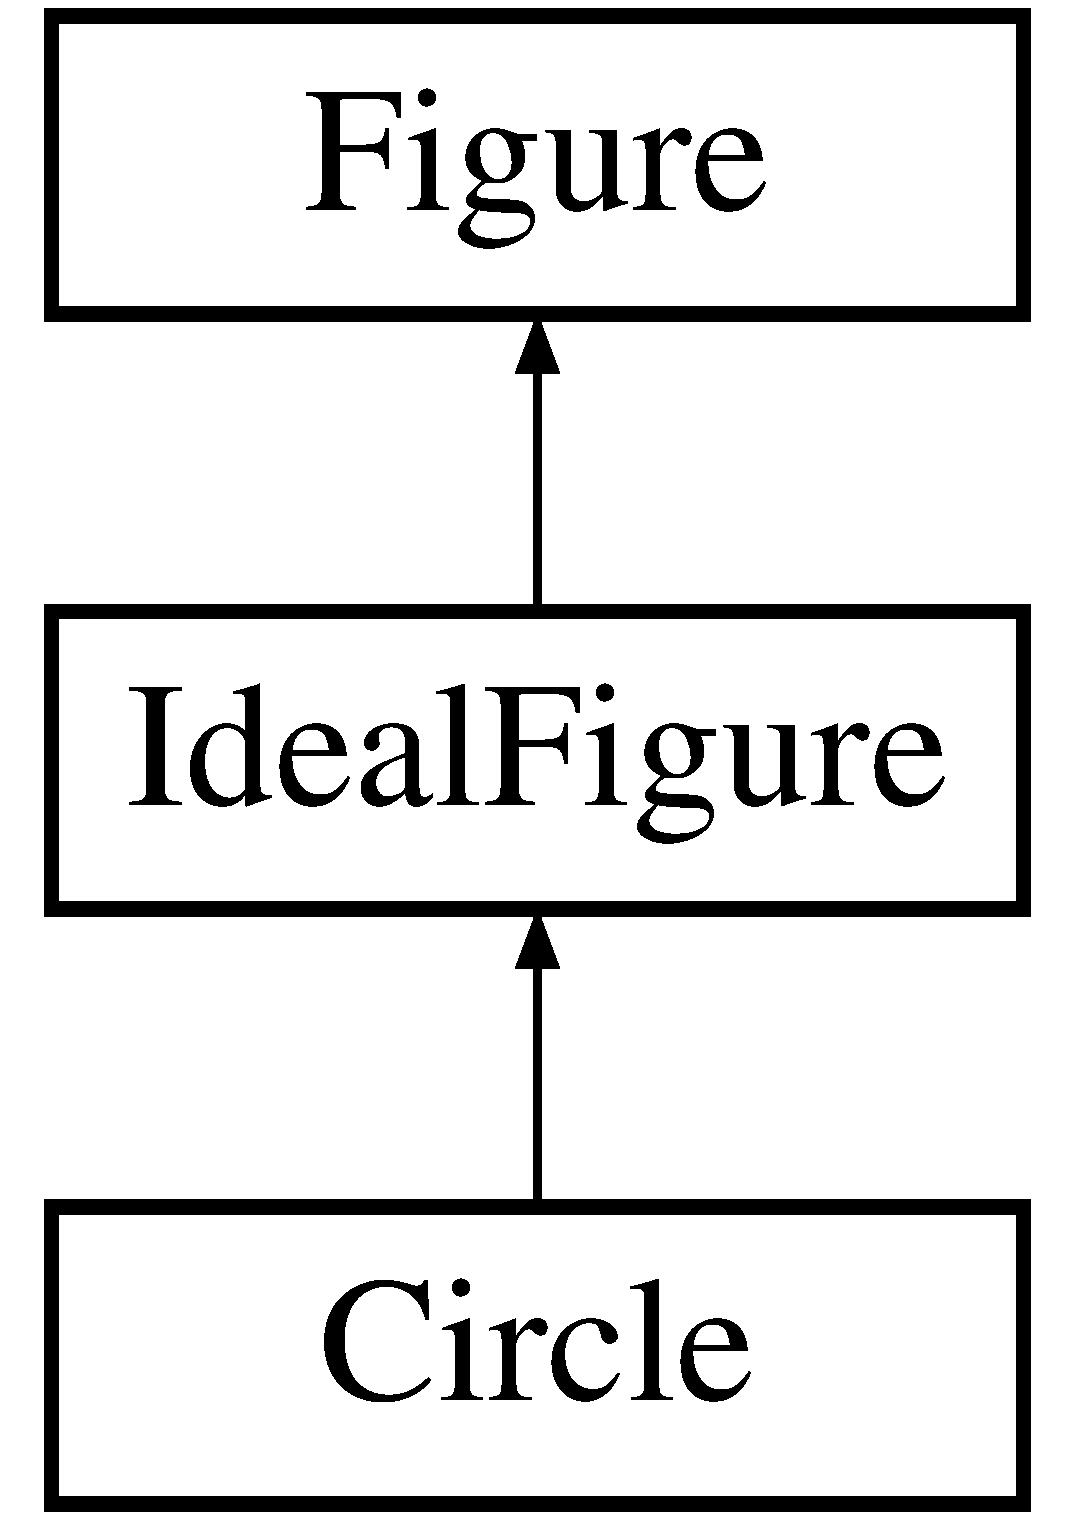
\includegraphics[height=3.000000cm]{class_circle}
\end{center}
\end{figure}
\subsection*{Public Member Functions}
\begin{DoxyCompactItemize}
\item 
\hyperlink{class_circle_a555b78514051debac82915e25ee37245}{Circle} (\hyperlink{class_point}{Point} origin=\hyperlink{class_point}{Point}(0, 0), double radius=0.\+0)
\item 
\hyperlink{class_circle_ae12be199f60ebd4fa356047faec83818}{Circle} (\hyperlink{class_point_a00b37528c0db634a12ecee9b29d79579}{Point\+::point\+Type} ox=0, \hyperlink{class_point_a00b37528c0db634a12ecee9b29d79579}{Point\+::point\+Type} oy=0, double radius=0)
\item 
\hyperlink{class_circle_ae3f30436e645d73e368e8ee55f8d1650}{$\sim$\+Circle} ()
\item 
double \hyperlink{class_circle_a4f31d14f360b6e1f1acfb283ad65145a}{area} ()
\item 
double \hyperlink{class_circle_ab0a4db4a814591918b0372feac5df46b}{perimeter} ()
\item 
\hyperlink{class_convex_polygon}{Convex\+Polygon} \hyperlink{class_circle_ae5f140e34baceae51bb662bc15a5cecc}{rasterize} (unsigned p\+\_\+resolution=\hyperlink{_ideal_figure_8h_a00d8c937c01b3a24f12056a00144690b}{I\+F\+\_\+\+R\+A\+S\+T\+E\+R\+\_\+\+R\+E\+Z\+O\+L\+U\+T\+I\+ON})
\item 
virtual \hyperlink{classtinyxml2_1_1_x_m_l_node}{tinyxml2\+::\+X\+M\+L\+Node} $\ast$ \hyperlink{class_circle_a86fa86f49342a310db5e717c75011487}{serialize} (\hyperlink{classtinyxml2_1_1_x_m_l_document}{tinyxml2\+::\+X\+M\+L\+Document} \&xml\+Doc)
\end{DoxyCompactItemize}
\subsection*{Additional Inherited Members}


\subsection{Constructor \& Destructor Documentation}
\mbox{\Hypertarget{class_circle_a555b78514051debac82915e25ee37245}\label{class_circle_a555b78514051debac82915e25ee37245}} 
\index{Circle@{Circle}!Circle@{Circle}}
\index{Circle@{Circle}!Circle@{Circle}}
\subsubsection{\texorpdfstring{Circle()}{Circle()}\hspace{0.1cm}{\footnotesize\ttfamily [1/2]}}
{\footnotesize\ttfamily Circle\+::\+Circle (\begin{DoxyParamCaption}\item[{\hyperlink{class_point}{Point}}]{origin = {\ttfamily \hyperlink{class_point}{Point}(0,~0)},  }\item[{double}]{radius = {\ttfamily 0.0} }\end{DoxyParamCaption})\hspace{0.3cm}{\ttfamily [inline]}}

\mbox{\Hypertarget{class_circle_ae12be199f60ebd4fa356047faec83818}\label{class_circle_ae12be199f60ebd4fa356047faec83818}} 
\index{Circle@{Circle}!Circle@{Circle}}
\index{Circle@{Circle}!Circle@{Circle}}
\subsubsection{\texorpdfstring{Circle()}{Circle()}\hspace{0.1cm}{\footnotesize\ttfamily [2/2]}}
{\footnotesize\ttfamily Circle\+::\+Circle (\begin{DoxyParamCaption}\item[{\hyperlink{class_point_a00b37528c0db634a12ecee9b29d79579}{Point\+::point\+Type}}]{ox = {\ttfamily 0},  }\item[{\hyperlink{class_point_a00b37528c0db634a12ecee9b29d79579}{Point\+::point\+Type}}]{oy = {\ttfamily 0},  }\item[{double}]{radius = {\ttfamily 0} }\end{DoxyParamCaption})\hspace{0.3cm}{\ttfamily [inline]}}

\mbox{\Hypertarget{class_circle_ae3f30436e645d73e368e8ee55f8d1650}\label{class_circle_ae3f30436e645d73e368e8ee55f8d1650}} 
\index{Circle@{Circle}!````~Circle@{$\sim$\+Circle}}
\index{````~Circle@{$\sim$\+Circle}!Circle@{Circle}}
\subsubsection{\texorpdfstring{$\sim$\+Circle()}{~Circle()}}
{\footnotesize\ttfamily Circle\+::$\sim$\+Circle (\begin{DoxyParamCaption}{ }\end{DoxyParamCaption})\hspace{0.3cm}{\ttfamily [inline]}}



\subsection{Member Function Documentation}
\mbox{\Hypertarget{class_circle_a4f31d14f360b6e1f1acfb283ad65145a}\label{class_circle_a4f31d14f360b6e1f1acfb283ad65145a}} 
\index{Circle@{Circle}!area@{area}}
\index{area@{area}!Circle@{Circle}}
\subsubsection{\texorpdfstring{area()}{area()}}
{\footnotesize\ttfamily double Circle\+::area (\begin{DoxyParamCaption}{ }\end{DoxyParamCaption})\hspace{0.3cm}{\ttfamily [virtual]}}



Implements \hyperlink{class_figure_a9860bda67fc9ce8127a812e167c4ce75}{Figure}.

\mbox{\Hypertarget{class_circle_ab0a4db4a814591918b0372feac5df46b}\label{class_circle_ab0a4db4a814591918b0372feac5df46b}} 
\index{Circle@{Circle}!perimeter@{perimeter}}
\index{perimeter@{perimeter}!Circle@{Circle}}
\subsubsection{\texorpdfstring{perimeter()}{perimeter()}}
{\footnotesize\ttfamily double Circle\+::perimeter (\begin{DoxyParamCaption}{ }\end{DoxyParamCaption})\hspace{0.3cm}{\ttfamily [virtual]}}



Implements \hyperlink{class_figure_acae6802e2a55b322f7566f313d474546}{Figure}.

\mbox{\Hypertarget{class_circle_ae5f140e34baceae51bb662bc15a5cecc}\label{class_circle_ae5f140e34baceae51bb662bc15a5cecc}} 
\index{Circle@{Circle}!rasterize@{rasterize}}
\index{rasterize@{rasterize}!Circle@{Circle}}
\subsubsection{\texorpdfstring{rasterize()}{rasterize()}}
{\footnotesize\ttfamily \hyperlink{class_convex_polygon}{Convex\+Polygon} Circle\+::rasterize (\begin{DoxyParamCaption}\item[{unsigned}]{rezolution = {\ttfamily \hyperlink{_ideal_figure_8h_a00d8c937c01b3a24f12056a00144690b}{I\+F\+\_\+\+R\+A\+S\+T\+E\+R\+\_\+\+R\+E\+Z\+O\+L\+U\+T\+I\+ON}} }\end{DoxyParamCaption})\hspace{0.3cm}{\ttfamily [virtual]}}

N\+O\+TE Functia nu pastreaza Aria/\+Perimetrul figurii dar este garantat ca va da tot timpul Un poligon convex inscris in figura data deci cu aria mai mica sau egala O valoare mai mare de 50 va da rezultate destul de bune dpdv vizual 

Implements \hyperlink{class_ideal_figure_ae1b50ae419aa258fb7ebc7131e3d4a5d}{Ideal\+Figure}.

\mbox{\Hypertarget{class_circle_a86fa86f49342a310db5e717c75011487}\label{class_circle_a86fa86f49342a310db5e717c75011487}} 
\index{Circle@{Circle}!serialize@{serialize}}
\index{serialize@{serialize}!Circle@{Circle}}
\subsubsection{\texorpdfstring{serialize()}{serialize()}}
{\footnotesize\ttfamily \hyperlink{classtinyxml2_1_1_x_m_l_node}{tinyxml2\+::\+X\+M\+L\+Node} $\ast$ Circle\+::serialize (\begin{DoxyParamCaption}\item[{\hyperlink{classtinyxml2_1_1_x_m_l_document}{tinyxml2\+::\+X\+M\+L\+Document} \&}]{xml\+Doc }\end{DoxyParamCaption})\hspace{0.3cm}{\ttfamily [virtual]}}



Reimplemented from \hyperlink{class_ideal_figure_a5a795a3de8992af3fb9cee4a904b31a5}{Ideal\+Figure}.



The documentation for this class was generated from the following files\+:\begin{DoxyCompactItemize}
\item 
\hyperlink{_circle_8h}{Circle.\+h}\item 
\hyperlink{_circle_8cpp}{Circle.\+cpp}\end{DoxyCompactItemize}

\hypertarget{class_convex_polygon}{}\section{Convex\+Polygon Class Reference}
\label{class_convex_polygon}\index{Convex\+Polygon@{Convex\+Polygon}}


{\ttfamily \#include $<$Convex\+Polygon.\+h$>$}

Inheritance diagram for Convex\+Polygon\+:\begin{figure}[H]
\begin{center}
\leavevmode
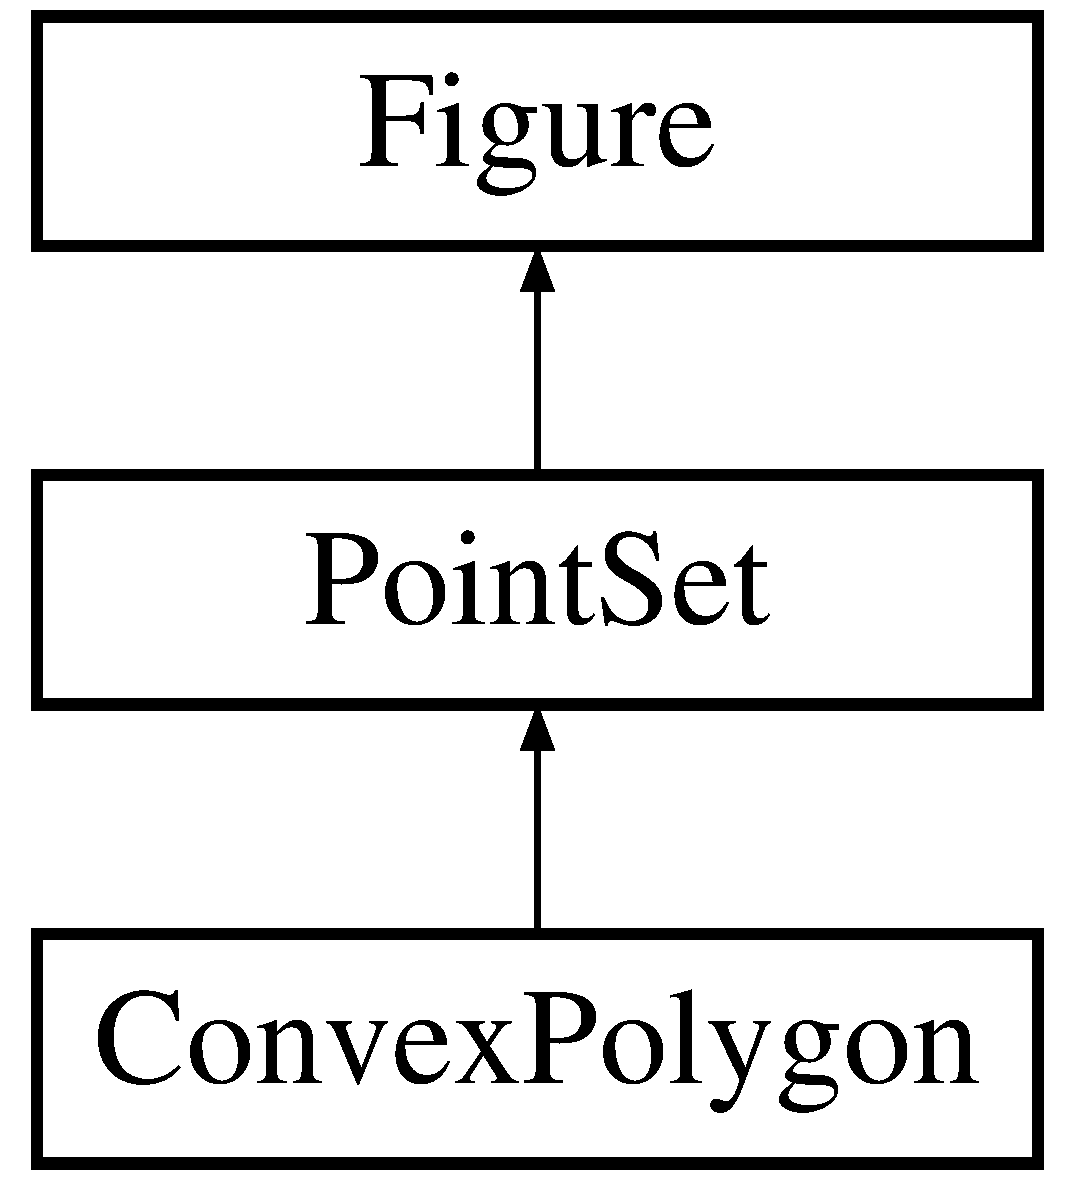
\includegraphics[height=3.000000cm]{class_convex_polygon}
\end{center}
\end{figure}
\subsection*{Public Member Functions}
\begin{DoxyCompactItemize}
\item 
\hyperlink{class_convex_polygon_aac5d610baed71675c395b4ef0898dfd2}{Convex\+Polygon} (\hyperlink{class_list}{List}$<$ \hyperlink{class_point}{Point} $>$ lst=\hyperlink{class_list}{List}$<$ \hyperlink{class_point}{Point} $>$(), unsigned lst\+\_\+count=0)
\item 
double \hyperlink{class_convex_polygon_a4d8ca9c4d454308dcd95ae9f9dee2688}{area} ()
\item 
double \hyperlink{class_convex_polygon_ac8e11403c36adb4ac51b6c169257b605}{perimeter} ()
\item 
virtual \hyperlink{classtinyxml2_1_1_x_m_l_node}{tinyxml2\+::\+X\+M\+L\+Node} $\ast$ \hyperlink{class_convex_polygon_ab7cfd51933dd7a3bf821056c292ca62c}{serialize} (\hyperlink{classtinyxml2_1_1_x_m_l_document}{tinyxml2\+::\+X\+M\+L\+Document} \&xml\+Doc)
\item 
void \hyperlink{class_convex_polygon_a6956c62f285204cec995cd0c3e7ed852}{dbg\+\_\+print\+\_\+points} (std\+::ostream \&g)
\end{DoxyCompactItemize}
\subsection*{Additional Inherited Members}


\subsection{Constructor \& Destructor Documentation}
\mbox{\Hypertarget{class_convex_polygon_aac5d610baed71675c395b4ef0898dfd2}\label{class_convex_polygon_aac5d610baed71675c395b4ef0898dfd2}} 
\index{Convex\+Polygon@{Convex\+Polygon}!Convex\+Polygon@{Convex\+Polygon}}
\index{Convex\+Polygon@{Convex\+Polygon}!Convex\+Polygon@{Convex\+Polygon}}
\subsubsection{\texorpdfstring{Convex\+Polygon()}{ConvexPolygon()}}
{\footnotesize\ttfamily Convex\+Polygon\+::\+Convex\+Polygon (\begin{DoxyParamCaption}\item[{\hyperlink{class_list}{List}$<$ \hyperlink{class_point}{Point} $>$}]{lst = {\ttfamily \hyperlink{class_list}{List}$<$\hyperlink{class_point}{Point}$>$()},  }\item[{unsigned}]{lst\+\_\+count = {\ttfamily 0} }\end{DoxyParamCaption})}



\subsection{Member Function Documentation}
\mbox{\Hypertarget{class_convex_polygon_a4d8ca9c4d454308dcd95ae9f9dee2688}\label{class_convex_polygon_a4d8ca9c4d454308dcd95ae9f9dee2688}} 
\index{Convex\+Polygon@{Convex\+Polygon}!area@{area}}
\index{area@{area}!Convex\+Polygon@{Convex\+Polygon}}
\subsubsection{\texorpdfstring{area()}{area()}}
{\footnotesize\ttfamily double Convex\+Polygon\+::area (\begin{DoxyParamCaption}{ }\end{DoxyParamCaption})\hspace{0.3cm}{\ttfamily [virtual]}}



Implements \hyperlink{class_figure_a9860bda67fc9ce8127a812e167c4ce75}{Figure}.

\mbox{\Hypertarget{class_convex_polygon_a6956c62f285204cec995cd0c3e7ed852}\label{class_convex_polygon_a6956c62f285204cec995cd0c3e7ed852}} 
\index{Convex\+Polygon@{Convex\+Polygon}!dbg\+\_\+print\+\_\+points@{dbg\+\_\+print\+\_\+points}}
\index{dbg\+\_\+print\+\_\+points@{dbg\+\_\+print\+\_\+points}!Convex\+Polygon@{Convex\+Polygon}}
\subsubsection{\texorpdfstring{dbg\+\_\+print\+\_\+points()}{dbg\_print\_points()}}
{\footnotesize\ttfamily void Convex\+Polygon\+::dbg\+\_\+print\+\_\+points (\begin{DoxyParamCaption}\item[{std\+::ostream \&}]{g }\end{DoxyParamCaption})}

\mbox{\Hypertarget{class_convex_polygon_ac8e11403c36adb4ac51b6c169257b605}\label{class_convex_polygon_ac8e11403c36adb4ac51b6c169257b605}} 
\index{Convex\+Polygon@{Convex\+Polygon}!perimeter@{perimeter}}
\index{perimeter@{perimeter}!Convex\+Polygon@{Convex\+Polygon}}
\subsubsection{\texorpdfstring{perimeter()}{perimeter()}}
{\footnotesize\ttfamily double Convex\+Polygon\+::perimeter (\begin{DoxyParamCaption}{ }\end{DoxyParamCaption})\hspace{0.3cm}{\ttfamily [virtual]}}



Implements \hyperlink{class_figure_acae6802e2a55b322f7566f313d474546}{Figure}.

\mbox{\Hypertarget{class_convex_polygon_ab7cfd51933dd7a3bf821056c292ca62c}\label{class_convex_polygon_ab7cfd51933dd7a3bf821056c292ca62c}} 
\index{Convex\+Polygon@{Convex\+Polygon}!serialize@{serialize}}
\index{serialize@{serialize}!Convex\+Polygon@{Convex\+Polygon}}
\subsubsection{\texorpdfstring{serialize()}{serialize()}}
{\footnotesize\ttfamily \hyperlink{classtinyxml2_1_1_x_m_l_node}{tinyxml2\+::\+X\+M\+L\+Node} $\ast$ Convex\+Polygon\+::serialize (\begin{DoxyParamCaption}\item[{\hyperlink{classtinyxml2_1_1_x_m_l_document}{tinyxml2\+::\+X\+M\+L\+Document} \&}]{xml\+Doc }\end{DoxyParamCaption})\hspace{0.3cm}{\ttfamily [virtual]}}



Reimplemented from \hyperlink{class_point_set_a282360046d7566f50d1ceec49aca0d89}{Point\+Set}.



The documentation for this class was generated from the following files\+:\begin{DoxyCompactItemize}
\item 
\hyperlink{_convex_polygon_8h}{Convex\+Polygon.\+h}\item 
\hyperlink{_convex_polygon_8cpp}{Convex\+Polygon.\+cpp}\end{DoxyCompactItemize}

\hypertarget{classtinyxml2_1_1_dyn_array}{}\section{tinyxml2\+:\+:Dyn\+Array$<$ T, I\+N\+I\+T\+I\+A\+L\+\_\+\+S\+I\+ZE $>$ Class Template Reference}
\label{classtinyxml2_1_1_dyn_array}\index{tinyxml2\+::\+Dyn\+Array$<$ T, I\+N\+I\+T\+I\+A\+L\+\_\+\+S\+I\+Z\+E $>$@{tinyxml2\+::\+Dyn\+Array$<$ T, I\+N\+I\+T\+I\+A\+L\+\_\+\+S\+I\+Z\+E $>$}}


{\ttfamily \#include $<$tinyxml2.\+h$>$}

\subsection*{Public Member Functions}
\begin{DoxyCompactItemize}
\item 
\hyperlink{classtinyxml2_1_1_dyn_array_aaad72f384e761c70a4519183eb8fea17}{Dyn\+Array} ()
\item 
\hyperlink{classtinyxml2_1_1_dyn_array_a4a6aefdca7fe0d3f4068e31870a5adee}{$\sim$\+Dyn\+Array} ()
\item 
void \hyperlink{classtinyxml2_1_1_dyn_array_af87a804cd831226d069274b44b74b8bc}{Clear} ()
\item 
void \hyperlink{classtinyxml2_1_1_dyn_array_aea7ffe983b5d3284bd43171afd7c99d0}{Push} (T t)
\item 
T $\ast$ \hyperlink{classtinyxml2_1_1_dyn_array_ad289abee8cd02b26e215f1b63d2043f1}{Push\+Arr} (int count)
\item 
T \hyperlink{classtinyxml2_1_1_dyn_array_a27a3f2f6f869815b6eabb3ea40cf0712}{Pop} ()
\item 
void \hyperlink{classtinyxml2_1_1_dyn_array_ab8b8c94a2312ab27e2846f0d61ef677a}{Pop\+Arr} (int count)
\item 
bool \hyperlink{classtinyxml2_1_1_dyn_array_a044fc26f44ed3e96ffaeac542188149e}{Empty} () const
\item 
T \& \hyperlink{classtinyxml2_1_1_dyn_array_a756cf4e7464c711aa720e2b17a251daa}{operator\mbox{[}$\,$\mbox{]}} (int i)
\item 
const T \& \hyperlink{classtinyxml2_1_1_dyn_array_a474a5cd9bc97ea32b3dcef4c773125e1}{operator\mbox{[}$\,$\mbox{]}} (int i) const
\item 
const T \& \hyperlink{classtinyxml2_1_1_dyn_array_a5e4e1e408e646688503dec77c77c9d59}{Peek\+Top} () const
\item 
int \hyperlink{classtinyxml2_1_1_dyn_array_a67614d80847eb92cab330f1a5849a9a2}{Size} () const
\item 
int \hyperlink{classtinyxml2_1_1_dyn_array_a8e101fdf5b4248ac119d7dca6d0f5421}{Capacity} () const
\item 
const T $\ast$ \hyperlink{classtinyxml2_1_1_dyn_array_a60b33e61cf10b3fd900ee46692dc0fe9}{Mem} () const
\item 
T $\ast$ \hyperlink{classtinyxml2_1_1_dyn_array_a2f0842cd666e2ad951f1a8bd6561fa40}{Mem} ()
\end{DoxyCompactItemize}


\subsection{Constructor \& Destructor Documentation}
\mbox{\Hypertarget{classtinyxml2_1_1_dyn_array_aaad72f384e761c70a4519183eb8fea17}\label{classtinyxml2_1_1_dyn_array_aaad72f384e761c70a4519183eb8fea17}} 
\index{tinyxml2\+::\+Dyn\+Array@{tinyxml2\+::\+Dyn\+Array}!Dyn\+Array@{Dyn\+Array}}
\index{Dyn\+Array@{Dyn\+Array}!tinyxml2\+::\+Dyn\+Array@{tinyxml2\+::\+Dyn\+Array}}
\subsubsection{\texorpdfstring{Dyn\+Array()}{DynArray()}}
{\footnotesize\ttfamily template$<$class T, int I\+N\+I\+T\+I\+A\+L\+\_\+\+S\+I\+ZE$>$ \\
\hyperlink{classtinyxml2_1_1_dyn_array}{tinyxml2\+::\+Dyn\+Array}$<$ T, I\+N\+I\+T\+I\+A\+L\+\_\+\+S\+I\+ZE $>$\+::\hyperlink{classtinyxml2_1_1_dyn_array}{Dyn\+Array} (\begin{DoxyParamCaption}{ }\end{DoxyParamCaption})\hspace{0.3cm}{\ttfamily [inline]}}

\mbox{\Hypertarget{classtinyxml2_1_1_dyn_array_a4a6aefdca7fe0d3f4068e31870a5adee}\label{classtinyxml2_1_1_dyn_array_a4a6aefdca7fe0d3f4068e31870a5adee}} 
\index{tinyxml2\+::\+Dyn\+Array@{tinyxml2\+::\+Dyn\+Array}!````~Dyn\+Array@{$\sim$\+Dyn\+Array}}
\index{````~Dyn\+Array@{$\sim$\+Dyn\+Array}!tinyxml2\+::\+Dyn\+Array@{tinyxml2\+::\+Dyn\+Array}}
\subsubsection{\texorpdfstring{$\sim$\+Dyn\+Array()}{~DynArray()}}
{\footnotesize\ttfamily template$<$class T, int I\+N\+I\+T\+I\+A\+L\+\_\+\+S\+I\+ZE$>$ \\
\hyperlink{classtinyxml2_1_1_dyn_array}{tinyxml2\+::\+Dyn\+Array}$<$ T, I\+N\+I\+T\+I\+A\+L\+\_\+\+S\+I\+ZE $>$\+::$\sim$\hyperlink{classtinyxml2_1_1_dyn_array}{Dyn\+Array} (\begin{DoxyParamCaption}{ }\end{DoxyParamCaption})\hspace{0.3cm}{\ttfamily [inline]}}



\subsection{Member Function Documentation}
\mbox{\Hypertarget{classtinyxml2_1_1_dyn_array_a8e101fdf5b4248ac119d7dca6d0f5421}\label{classtinyxml2_1_1_dyn_array_a8e101fdf5b4248ac119d7dca6d0f5421}} 
\index{tinyxml2\+::\+Dyn\+Array@{tinyxml2\+::\+Dyn\+Array}!Capacity@{Capacity}}
\index{Capacity@{Capacity}!tinyxml2\+::\+Dyn\+Array@{tinyxml2\+::\+Dyn\+Array}}
\subsubsection{\texorpdfstring{Capacity()}{Capacity()}}
{\footnotesize\ttfamily template$<$class T, int I\+N\+I\+T\+I\+A\+L\+\_\+\+S\+I\+ZE$>$ \\
int \hyperlink{classtinyxml2_1_1_dyn_array}{tinyxml2\+::\+Dyn\+Array}$<$ T, I\+N\+I\+T\+I\+A\+L\+\_\+\+S\+I\+ZE $>$\+::Capacity (\begin{DoxyParamCaption}{ }\end{DoxyParamCaption}) const\hspace{0.3cm}{\ttfamily [inline]}}

\mbox{\Hypertarget{classtinyxml2_1_1_dyn_array_af87a804cd831226d069274b44b74b8bc}\label{classtinyxml2_1_1_dyn_array_af87a804cd831226d069274b44b74b8bc}} 
\index{tinyxml2\+::\+Dyn\+Array@{tinyxml2\+::\+Dyn\+Array}!Clear@{Clear}}
\index{Clear@{Clear}!tinyxml2\+::\+Dyn\+Array@{tinyxml2\+::\+Dyn\+Array}}
\subsubsection{\texorpdfstring{Clear()}{Clear()}}
{\footnotesize\ttfamily template$<$class T, int I\+N\+I\+T\+I\+A\+L\+\_\+\+S\+I\+ZE$>$ \\
void \hyperlink{classtinyxml2_1_1_dyn_array}{tinyxml2\+::\+Dyn\+Array}$<$ T, I\+N\+I\+T\+I\+A\+L\+\_\+\+S\+I\+ZE $>$\+::Clear (\begin{DoxyParamCaption}{ }\end{DoxyParamCaption})\hspace{0.3cm}{\ttfamily [inline]}}

\mbox{\Hypertarget{classtinyxml2_1_1_dyn_array_a044fc26f44ed3e96ffaeac542188149e}\label{classtinyxml2_1_1_dyn_array_a044fc26f44ed3e96ffaeac542188149e}} 
\index{tinyxml2\+::\+Dyn\+Array@{tinyxml2\+::\+Dyn\+Array}!Empty@{Empty}}
\index{Empty@{Empty}!tinyxml2\+::\+Dyn\+Array@{tinyxml2\+::\+Dyn\+Array}}
\subsubsection{\texorpdfstring{Empty()}{Empty()}}
{\footnotesize\ttfamily template$<$class T, int I\+N\+I\+T\+I\+A\+L\+\_\+\+S\+I\+ZE$>$ \\
bool \hyperlink{classtinyxml2_1_1_dyn_array}{tinyxml2\+::\+Dyn\+Array}$<$ T, I\+N\+I\+T\+I\+A\+L\+\_\+\+S\+I\+ZE $>$\+::Empty (\begin{DoxyParamCaption}{ }\end{DoxyParamCaption}) const\hspace{0.3cm}{\ttfamily [inline]}}

\mbox{\Hypertarget{classtinyxml2_1_1_dyn_array_a60b33e61cf10b3fd900ee46692dc0fe9}\label{classtinyxml2_1_1_dyn_array_a60b33e61cf10b3fd900ee46692dc0fe9}} 
\index{tinyxml2\+::\+Dyn\+Array@{tinyxml2\+::\+Dyn\+Array}!Mem@{Mem}}
\index{Mem@{Mem}!tinyxml2\+::\+Dyn\+Array@{tinyxml2\+::\+Dyn\+Array}}
\subsubsection{\texorpdfstring{Mem()}{Mem()}\hspace{0.1cm}{\footnotesize\ttfamily [1/2]}}
{\footnotesize\ttfamily template$<$class T, int I\+N\+I\+T\+I\+A\+L\+\_\+\+S\+I\+ZE$>$ \\
const T$\ast$ \hyperlink{classtinyxml2_1_1_dyn_array}{tinyxml2\+::\+Dyn\+Array}$<$ T, I\+N\+I\+T\+I\+A\+L\+\_\+\+S\+I\+ZE $>$\+::Mem (\begin{DoxyParamCaption}{ }\end{DoxyParamCaption}) const\hspace{0.3cm}{\ttfamily [inline]}}

\mbox{\Hypertarget{classtinyxml2_1_1_dyn_array_a2f0842cd666e2ad951f1a8bd6561fa40}\label{classtinyxml2_1_1_dyn_array_a2f0842cd666e2ad951f1a8bd6561fa40}} 
\index{tinyxml2\+::\+Dyn\+Array@{tinyxml2\+::\+Dyn\+Array}!Mem@{Mem}}
\index{Mem@{Mem}!tinyxml2\+::\+Dyn\+Array@{tinyxml2\+::\+Dyn\+Array}}
\subsubsection{\texorpdfstring{Mem()}{Mem()}\hspace{0.1cm}{\footnotesize\ttfamily [2/2]}}
{\footnotesize\ttfamily template$<$class T, int I\+N\+I\+T\+I\+A\+L\+\_\+\+S\+I\+ZE$>$ \\
T$\ast$ \hyperlink{classtinyxml2_1_1_dyn_array}{tinyxml2\+::\+Dyn\+Array}$<$ T, I\+N\+I\+T\+I\+A\+L\+\_\+\+S\+I\+ZE $>$\+::Mem (\begin{DoxyParamCaption}{ }\end{DoxyParamCaption})\hspace{0.3cm}{\ttfamily [inline]}}

\mbox{\Hypertarget{classtinyxml2_1_1_dyn_array_a756cf4e7464c711aa720e2b17a251daa}\label{classtinyxml2_1_1_dyn_array_a756cf4e7464c711aa720e2b17a251daa}} 
\index{tinyxml2\+::\+Dyn\+Array@{tinyxml2\+::\+Dyn\+Array}!operator\mbox{[}\mbox{]}@{operator[]}}
\index{operator\mbox{[}\mbox{]}@{operator[]}!tinyxml2\+::\+Dyn\+Array@{tinyxml2\+::\+Dyn\+Array}}
\subsubsection{\texorpdfstring{operator[]()}{operator[]()}\hspace{0.1cm}{\footnotesize\ttfamily [1/2]}}
{\footnotesize\ttfamily template$<$class T, int I\+N\+I\+T\+I\+A\+L\+\_\+\+S\+I\+ZE$>$ \\
T\& \hyperlink{classtinyxml2_1_1_dyn_array}{tinyxml2\+::\+Dyn\+Array}$<$ T, I\+N\+I\+T\+I\+A\+L\+\_\+\+S\+I\+ZE $>$\+::operator\mbox{[}$\,$\mbox{]} (\begin{DoxyParamCaption}\item[{int}]{i }\end{DoxyParamCaption})\hspace{0.3cm}{\ttfamily [inline]}}

\mbox{\Hypertarget{classtinyxml2_1_1_dyn_array_a474a5cd9bc97ea32b3dcef4c773125e1}\label{classtinyxml2_1_1_dyn_array_a474a5cd9bc97ea32b3dcef4c773125e1}} 
\index{tinyxml2\+::\+Dyn\+Array@{tinyxml2\+::\+Dyn\+Array}!operator\mbox{[}\mbox{]}@{operator[]}}
\index{operator\mbox{[}\mbox{]}@{operator[]}!tinyxml2\+::\+Dyn\+Array@{tinyxml2\+::\+Dyn\+Array}}
\subsubsection{\texorpdfstring{operator[]()}{operator[]()}\hspace{0.1cm}{\footnotesize\ttfamily [2/2]}}
{\footnotesize\ttfamily template$<$class T, int I\+N\+I\+T\+I\+A\+L\+\_\+\+S\+I\+ZE$>$ \\
const T\& \hyperlink{classtinyxml2_1_1_dyn_array}{tinyxml2\+::\+Dyn\+Array}$<$ T, I\+N\+I\+T\+I\+A\+L\+\_\+\+S\+I\+ZE $>$\+::operator\mbox{[}$\,$\mbox{]} (\begin{DoxyParamCaption}\item[{int}]{i }\end{DoxyParamCaption}) const\hspace{0.3cm}{\ttfamily [inline]}}

\mbox{\Hypertarget{classtinyxml2_1_1_dyn_array_a5e4e1e408e646688503dec77c77c9d59}\label{classtinyxml2_1_1_dyn_array_a5e4e1e408e646688503dec77c77c9d59}} 
\index{tinyxml2\+::\+Dyn\+Array@{tinyxml2\+::\+Dyn\+Array}!Peek\+Top@{Peek\+Top}}
\index{Peek\+Top@{Peek\+Top}!tinyxml2\+::\+Dyn\+Array@{tinyxml2\+::\+Dyn\+Array}}
\subsubsection{\texorpdfstring{Peek\+Top()}{PeekTop()}}
{\footnotesize\ttfamily template$<$class T, int I\+N\+I\+T\+I\+A\+L\+\_\+\+S\+I\+ZE$>$ \\
const T\& \hyperlink{classtinyxml2_1_1_dyn_array}{tinyxml2\+::\+Dyn\+Array}$<$ T, I\+N\+I\+T\+I\+A\+L\+\_\+\+S\+I\+ZE $>$\+::Peek\+Top (\begin{DoxyParamCaption}{ }\end{DoxyParamCaption}) const\hspace{0.3cm}{\ttfamily [inline]}}

\mbox{\Hypertarget{classtinyxml2_1_1_dyn_array_a27a3f2f6f869815b6eabb3ea40cf0712}\label{classtinyxml2_1_1_dyn_array_a27a3f2f6f869815b6eabb3ea40cf0712}} 
\index{tinyxml2\+::\+Dyn\+Array@{tinyxml2\+::\+Dyn\+Array}!Pop@{Pop}}
\index{Pop@{Pop}!tinyxml2\+::\+Dyn\+Array@{tinyxml2\+::\+Dyn\+Array}}
\subsubsection{\texorpdfstring{Pop()}{Pop()}}
{\footnotesize\ttfamily template$<$class T, int I\+N\+I\+T\+I\+A\+L\+\_\+\+S\+I\+ZE$>$ \\
T \hyperlink{classtinyxml2_1_1_dyn_array}{tinyxml2\+::\+Dyn\+Array}$<$ T, I\+N\+I\+T\+I\+A\+L\+\_\+\+S\+I\+ZE $>$\+::Pop (\begin{DoxyParamCaption}{ }\end{DoxyParamCaption})\hspace{0.3cm}{\ttfamily [inline]}}

\mbox{\Hypertarget{classtinyxml2_1_1_dyn_array_ab8b8c94a2312ab27e2846f0d61ef677a}\label{classtinyxml2_1_1_dyn_array_ab8b8c94a2312ab27e2846f0d61ef677a}} 
\index{tinyxml2\+::\+Dyn\+Array@{tinyxml2\+::\+Dyn\+Array}!Pop\+Arr@{Pop\+Arr}}
\index{Pop\+Arr@{Pop\+Arr}!tinyxml2\+::\+Dyn\+Array@{tinyxml2\+::\+Dyn\+Array}}
\subsubsection{\texorpdfstring{Pop\+Arr()}{PopArr()}}
{\footnotesize\ttfamily template$<$class T, int I\+N\+I\+T\+I\+A\+L\+\_\+\+S\+I\+ZE$>$ \\
void \hyperlink{classtinyxml2_1_1_dyn_array}{tinyxml2\+::\+Dyn\+Array}$<$ T, I\+N\+I\+T\+I\+A\+L\+\_\+\+S\+I\+ZE $>$\+::Pop\+Arr (\begin{DoxyParamCaption}\item[{int}]{count }\end{DoxyParamCaption})\hspace{0.3cm}{\ttfamily [inline]}}

\mbox{\Hypertarget{classtinyxml2_1_1_dyn_array_aea7ffe983b5d3284bd43171afd7c99d0}\label{classtinyxml2_1_1_dyn_array_aea7ffe983b5d3284bd43171afd7c99d0}} 
\index{tinyxml2\+::\+Dyn\+Array@{tinyxml2\+::\+Dyn\+Array}!Push@{Push}}
\index{Push@{Push}!tinyxml2\+::\+Dyn\+Array@{tinyxml2\+::\+Dyn\+Array}}
\subsubsection{\texorpdfstring{Push()}{Push()}}
{\footnotesize\ttfamily template$<$class T, int I\+N\+I\+T\+I\+A\+L\+\_\+\+S\+I\+ZE$>$ \\
void \hyperlink{classtinyxml2_1_1_dyn_array}{tinyxml2\+::\+Dyn\+Array}$<$ T, I\+N\+I\+T\+I\+A\+L\+\_\+\+S\+I\+ZE $>$\+::Push (\begin{DoxyParamCaption}\item[{T}]{t }\end{DoxyParamCaption})\hspace{0.3cm}{\ttfamily [inline]}}

\mbox{\Hypertarget{classtinyxml2_1_1_dyn_array_ad289abee8cd02b26e215f1b63d2043f1}\label{classtinyxml2_1_1_dyn_array_ad289abee8cd02b26e215f1b63d2043f1}} 
\index{tinyxml2\+::\+Dyn\+Array@{tinyxml2\+::\+Dyn\+Array}!Push\+Arr@{Push\+Arr}}
\index{Push\+Arr@{Push\+Arr}!tinyxml2\+::\+Dyn\+Array@{tinyxml2\+::\+Dyn\+Array}}
\subsubsection{\texorpdfstring{Push\+Arr()}{PushArr()}}
{\footnotesize\ttfamily template$<$class T, int I\+N\+I\+T\+I\+A\+L\+\_\+\+S\+I\+ZE$>$ \\
T$\ast$ \hyperlink{classtinyxml2_1_1_dyn_array}{tinyxml2\+::\+Dyn\+Array}$<$ T, I\+N\+I\+T\+I\+A\+L\+\_\+\+S\+I\+ZE $>$\+::Push\+Arr (\begin{DoxyParamCaption}\item[{int}]{count }\end{DoxyParamCaption})\hspace{0.3cm}{\ttfamily [inline]}}

\mbox{\Hypertarget{classtinyxml2_1_1_dyn_array_a67614d80847eb92cab330f1a5849a9a2}\label{classtinyxml2_1_1_dyn_array_a67614d80847eb92cab330f1a5849a9a2}} 
\index{tinyxml2\+::\+Dyn\+Array@{tinyxml2\+::\+Dyn\+Array}!Size@{Size}}
\index{Size@{Size}!tinyxml2\+::\+Dyn\+Array@{tinyxml2\+::\+Dyn\+Array}}
\subsubsection{\texorpdfstring{Size()}{Size()}}
{\footnotesize\ttfamily template$<$class T, int I\+N\+I\+T\+I\+A\+L\+\_\+\+S\+I\+ZE$>$ \\
int \hyperlink{classtinyxml2_1_1_dyn_array}{tinyxml2\+::\+Dyn\+Array}$<$ T, I\+N\+I\+T\+I\+A\+L\+\_\+\+S\+I\+ZE $>$\+::Size (\begin{DoxyParamCaption}{ }\end{DoxyParamCaption}) const\hspace{0.3cm}{\ttfamily [inline]}}



The documentation for this class was generated from the following file\+:\begin{DoxyCompactItemize}
\item 
\hyperlink{tinyxml2_8h}{tinyxml2.\+h}\end{DoxyCompactItemize}

\hypertarget{class_ellipse}{}\section{Ellipse Class Reference}
\label{class_ellipse}\index{Ellipse@{Ellipse}}


{\ttfamily \#include $<$Ellipse.\+h$>$}

Inheritance diagram for Ellipse\+:\begin{figure}[H]
\begin{center}
\leavevmode
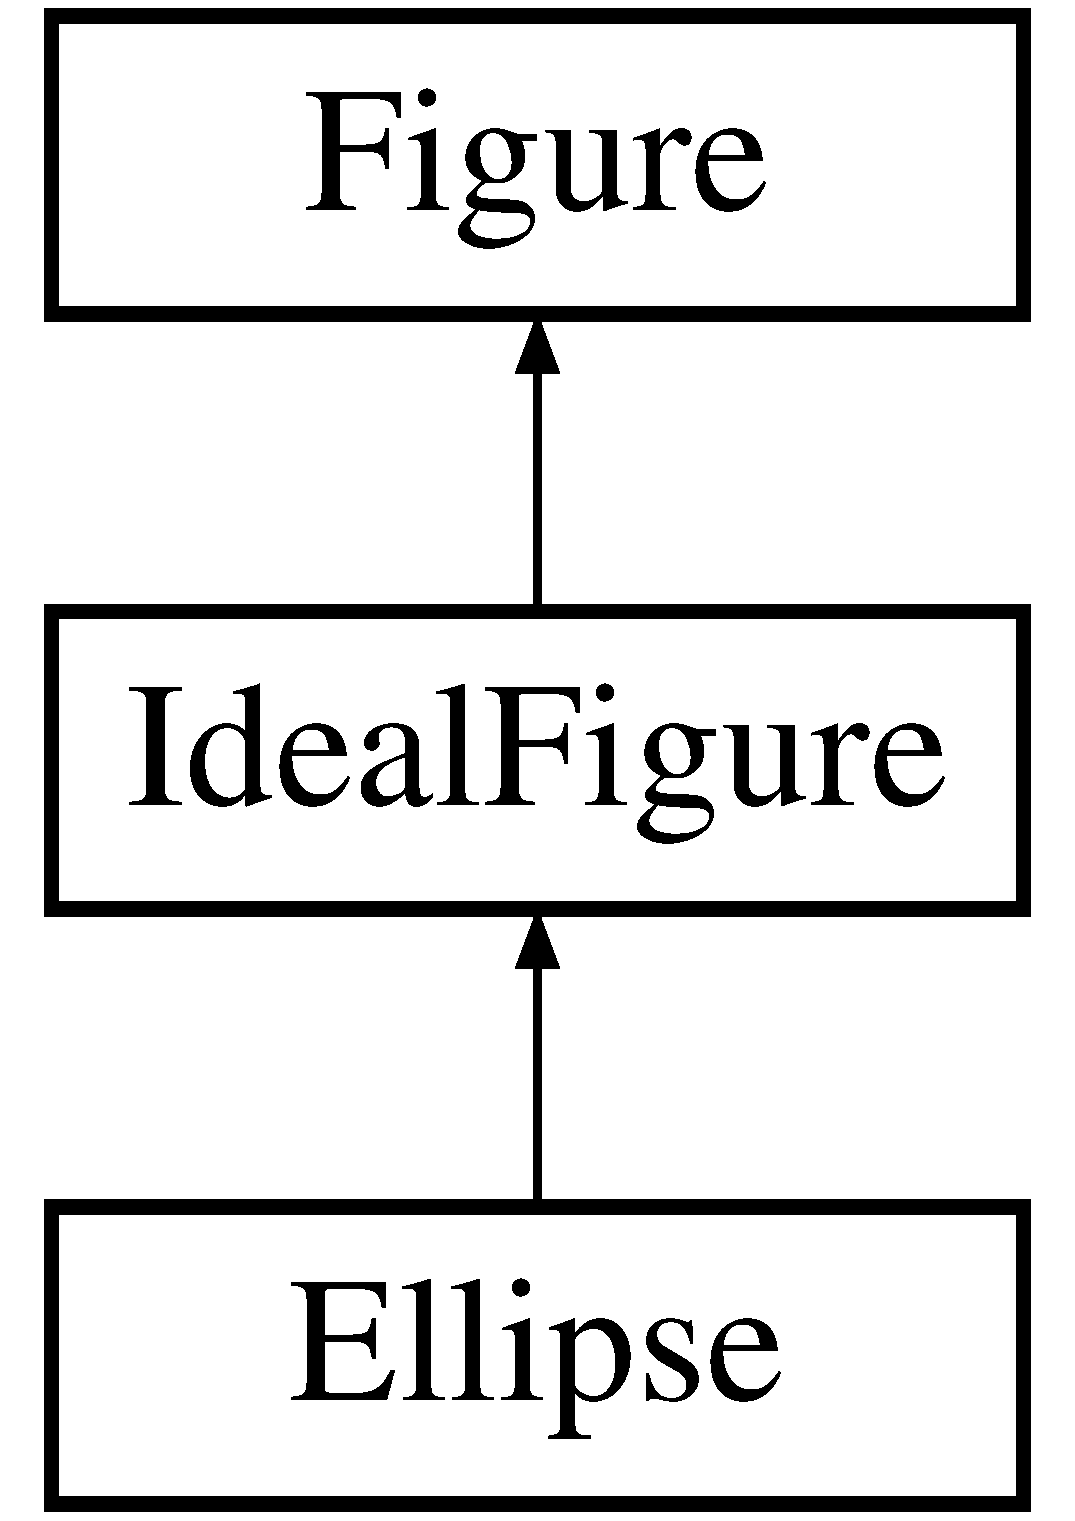
\includegraphics[height=3.000000cm]{class_ellipse}
\end{center}
\end{figure}
\subsection*{Public Member Functions}
\begin{DoxyCompactItemize}
\item 
\hyperlink{class_ellipse_a8b1d116bc30be65369b4db5b9b1c5f9d}{Ellipse} (\hyperlink{class_point}{Point} origin=\hyperlink{class_point}{Point}(0, 0), double a\+\_\+axis=0.\+0, double b\+\_\+axis=0.\+0)
\item 
\hyperlink{class_ellipse_a10da17fc6ffc0ea3590da040b42960e4}{Ellipse} (double x\+\_\+origin=0.\+0, double y\+\_\+origin=0.\+0, double a\+\_\+axis=0.\+0, double b\+\_\+axis=0.\+0)
\item 
\hyperlink{class_ellipse_a94271a8a2b16101a52491b7e81e28547}{$\sim$\+Ellipse} ()
\item 
double \hyperlink{class_ellipse_ad3de2759830df27c4ae1e65ecf46e7a1}{area} ()
\item 
double \hyperlink{class_ellipse_a367ca002c3a95761d0b913f98bc4eb6e}{perimeter} ()
\item 
\hyperlink{class_convex_polygon}{Convex\+Polygon} \hyperlink{class_ellipse_a54a8e6dab13f9d3a0cc633101e2ce6d6}{rasterize} (unsigned p\+\_\+resolution=\hyperlink{_ideal_figure_8h_a00d8c937c01b3a24f12056a00144690b}{I\+F\+\_\+\+R\+A\+S\+T\+E\+R\+\_\+\+R\+E\+Z\+O\+L\+U\+T\+I\+ON})
\item 
virtual \hyperlink{classtinyxml2_1_1_x_m_l_node}{tinyxml2\+::\+X\+M\+L\+Node} $\ast$ \hyperlink{class_ellipse_ab6c64b8c54cb74a4552a5f4f487f8d7d}{serialize} (\hyperlink{classtinyxml2_1_1_x_m_l_document}{tinyxml2\+::\+X\+M\+L\+Document} \&xml\+Doc)
\end{DoxyCompactItemize}
\subsection*{Additional Inherited Members}


\subsection{Constructor \& Destructor Documentation}
\mbox{\Hypertarget{class_ellipse_a8b1d116bc30be65369b4db5b9b1c5f9d}\label{class_ellipse_a8b1d116bc30be65369b4db5b9b1c5f9d}} 
\index{Ellipse@{Ellipse}!Ellipse@{Ellipse}}
\index{Ellipse@{Ellipse}!Ellipse@{Ellipse}}
\subsubsection{\texorpdfstring{Ellipse()}{Ellipse()}\hspace{0.1cm}{\footnotesize\ttfamily [1/2]}}
{\footnotesize\ttfamily Ellipse\+::\+Ellipse (\begin{DoxyParamCaption}\item[{\hyperlink{class_point}{Point}}]{origin = {\ttfamily \hyperlink{class_point}{Point}(0,~0)},  }\item[{double}]{a\+\_\+axis = {\ttfamily 0.0},  }\item[{double}]{b\+\_\+axis = {\ttfamily 0.0} }\end{DoxyParamCaption})\hspace{0.3cm}{\ttfamily [inline]}}

\mbox{\Hypertarget{class_ellipse_a10da17fc6ffc0ea3590da040b42960e4}\label{class_ellipse_a10da17fc6ffc0ea3590da040b42960e4}} 
\index{Ellipse@{Ellipse}!Ellipse@{Ellipse}}
\index{Ellipse@{Ellipse}!Ellipse@{Ellipse}}
\subsubsection{\texorpdfstring{Ellipse()}{Ellipse()}\hspace{0.1cm}{\footnotesize\ttfamily [2/2]}}
{\footnotesize\ttfamily Ellipse\+::\+Ellipse (\begin{DoxyParamCaption}\item[{double}]{x\+\_\+origin = {\ttfamily 0.0},  }\item[{double}]{y\+\_\+origin = {\ttfamily 0.0},  }\item[{double}]{a\+\_\+axis = {\ttfamily 0.0},  }\item[{double}]{b\+\_\+axis = {\ttfamily 0.0} }\end{DoxyParamCaption})\hspace{0.3cm}{\ttfamily [inline]}}

\mbox{\Hypertarget{class_ellipse_a94271a8a2b16101a52491b7e81e28547}\label{class_ellipse_a94271a8a2b16101a52491b7e81e28547}} 
\index{Ellipse@{Ellipse}!````~Ellipse@{$\sim$\+Ellipse}}
\index{````~Ellipse@{$\sim$\+Ellipse}!Ellipse@{Ellipse}}
\subsubsection{\texorpdfstring{$\sim$\+Ellipse()}{~Ellipse()}}
{\footnotesize\ttfamily Ellipse\+::$\sim$\+Ellipse (\begin{DoxyParamCaption}{ }\end{DoxyParamCaption})\hspace{0.3cm}{\ttfamily [inline]}}



\subsection{Member Function Documentation}
\mbox{\Hypertarget{class_ellipse_ad3de2759830df27c4ae1e65ecf46e7a1}\label{class_ellipse_ad3de2759830df27c4ae1e65ecf46e7a1}} 
\index{Ellipse@{Ellipse}!area@{area}}
\index{area@{area}!Ellipse@{Ellipse}}
\subsubsection{\texorpdfstring{area()}{area()}}
{\footnotesize\ttfamily double Ellipse\+::area (\begin{DoxyParamCaption}{ }\end{DoxyParamCaption})\hspace{0.3cm}{\ttfamily [virtual]}}



Implements \hyperlink{class_figure_a9860bda67fc9ce8127a812e167c4ce75}{Figure}.

\mbox{\Hypertarget{class_ellipse_a367ca002c3a95761d0b913f98bc4eb6e}\label{class_ellipse_a367ca002c3a95761d0b913f98bc4eb6e}} 
\index{Ellipse@{Ellipse}!perimeter@{perimeter}}
\index{perimeter@{perimeter}!Ellipse@{Ellipse}}
\subsubsection{\texorpdfstring{perimeter()}{perimeter()}}
{\footnotesize\ttfamily double Ellipse\+::perimeter (\begin{DoxyParamCaption}{ }\end{DoxyParamCaption})\hspace{0.3cm}{\ttfamily [virtual]}}



Implements \hyperlink{class_figure_acae6802e2a55b322f7566f313d474546}{Figure}.

\mbox{\Hypertarget{class_ellipse_a54a8e6dab13f9d3a0cc633101e2ce6d6}\label{class_ellipse_a54a8e6dab13f9d3a0cc633101e2ce6d6}} 
\index{Ellipse@{Ellipse}!rasterize@{rasterize}}
\index{rasterize@{rasterize}!Ellipse@{Ellipse}}
\subsubsection{\texorpdfstring{rasterize()}{rasterize()}}
{\footnotesize\ttfamily \hyperlink{class_convex_polygon}{Convex\+Polygon} Ellipse\+::rasterize (\begin{DoxyParamCaption}\item[{unsigned}]{rezolution = {\ttfamily \hyperlink{_ideal_figure_8h_a00d8c937c01b3a24f12056a00144690b}{I\+F\+\_\+\+R\+A\+S\+T\+E\+R\+\_\+\+R\+E\+Z\+O\+L\+U\+T\+I\+ON}} }\end{DoxyParamCaption})\hspace{0.3cm}{\ttfamily [virtual]}}

N\+O\+TE Functia nu pastreaza Aria/\+Perimetrul figurii dar este garantat ca va da tot timpul Un poligon convex inscris in figura data deci cu aria mai mica sau egala O valoare mai mare de 50 va da rezultate destul de bune dpdv vizual 

Implements \hyperlink{class_ideal_figure_ae1b50ae419aa258fb7ebc7131e3d4a5d}{Ideal\+Figure}.

\mbox{\Hypertarget{class_ellipse_ab6c64b8c54cb74a4552a5f4f487f8d7d}\label{class_ellipse_ab6c64b8c54cb74a4552a5f4f487f8d7d}} 
\index{Ellipse@{Ellipse}!serialize@{serialize}}
\index{serialize@{serialize}!Ellipse@{Ellipse}}
\subsubsection{\texorpdfstring{serialize()}{serialize()}}
{\footnotesize\ttfamily \hyperlink{classtinyxml2_1_1_x_m_l_node}{tinyxml2\+::\+X\+M\+L\+Node} $\ast$ Ellipse\+::serialize (\begin{DoxyParamCaption}\item[{\hyperlink{classtinyxml2_1_1_x_m_l_document}{tinyxml2\+::\+X\+M\+L\+Document} \&}]{xml\+Doc }\end{DoxyParamCaption})\hspace{0.3cm}{\ttfamily [virtual]}}



Reimplemented from \hyperlink{class_ideal_figure_a5a795a3de8992af3fb9cee4a904b31a5}{Ideal\+Figure}.



The documentation for this class was generated from the following files\+:\begin{DoxyCompactItemize}
\item 
\hyperlink{_ellipse_8h}{Ellipse.\+h}\item 
\hyperlink{_ellipse_8cpp}{Ellipse.\+cpp}\end{DoxyCompactItemize}

\hypertarget{structtinyxml2_1_1_entity}{}\section{tinyxml2\+:\+:Entity Struct Reference}
\label{structtinyxml2_1_1_entity}\index{tinyxml2\+::\+Entity@{tinyxml2\+::\+Entity}}
\subsection*{Public Attributes}
\begin{DoxyCompactItemize}
\item 
const char $\ast$ \hyperlink{structtinyxml2_1_1_entity_ab330f5d665d29bfc811ecfa76315894b}{pattern}
\item 
int \hyperlink{structtinyxml2_1_1_entity_a25e2b57cb59cb4fa68f283d7cb570f21}{length}
\item 
char \hyperlink{structtinyxml2_1_1_entity_a7334e81e33b4615655a403711b24f3ed}{value}
\end{DoxyCompactItemize}


\subsection{Member Data Documentation}
\mbox{\Hypertarget{structtinyxml2_1_1_entity_a25e2b57cb59cb4fa68f283d7cb570f21}\label{structtinyxml2_1_1_entity_a25e2b57cb59cb4fa68f283d7cb570f21}} 
\index{tinyxml2\+::\+Entity@{tinyxml2\+::\+Entity}!length@{length}}
\index{length@{length}!tinyxml2\+::\+Entity@{tinyxml2\+::\+Entity}}
\subsubsection{\texorpdfstring{length}{length}}
{\footnotesize\ttfamily int tinyxml2\+::\+Entity\+::length}

\mbox{\Hypertarget{structtinyxml2_1_1_entity_ab330f5d665d29bfc811ecfa76315894b}\label{structtinyxml2_1_1_entity_ab330f5d665d29bfc811ecfa76315894b}} 
\index{tinyxml2\+::\+Entity@{tinyxml2\+::\+Entity}!pattern@{pattern}}
\index{pattern@{pattern}!tinyxml2\+::\+Entity@{tinyxml2\+::\+Entity}}
\subsubsection{\texorpdfstring{pattern}{pattern}}
{\footnotesize\ttfamily const char$\ast$ tinyxml2\+::\+Entity\+::pattern}

\mbox{\Hypertarget{structtinyxml2_1_1_entity_a7334e81e33b4615655a403711b24f3ed}\label{structtinyxml2_1_1_entity_a7334e81e33b4615655a403711b24f3ed}} 
\index{tinyxml2\+::\+Entity@{tinyxml2\+::\+Entity}!value@{value}}
\index{value@{value}!tinyxml2\+::\+Entity@{tinyxml2\+::\+Entity}}
\subsubsection{\texorpdfstring{value}{value}}
{\footnotesize\ttfamily char tinyxml2\+::\+Entity\+::value}



The documentation for this struct was generated from the following file\+:\begin{DoxyCompactItemize}
\item 
\hyperlink{tinyxml2_8cpp}{tinyxml2.\+cpp}\end{DoxyCompactItemize}

\hypertarget{class_figure}{}\section{Figure Class Reference}
\label{class_figure}\index{Figure@{Figure}}


{\ttfamily \#include $<$Figure.\+h$>$}

Inheritance diagram for Figure\+:\begin{figure}[H]
\begin{center}
\leavevmode
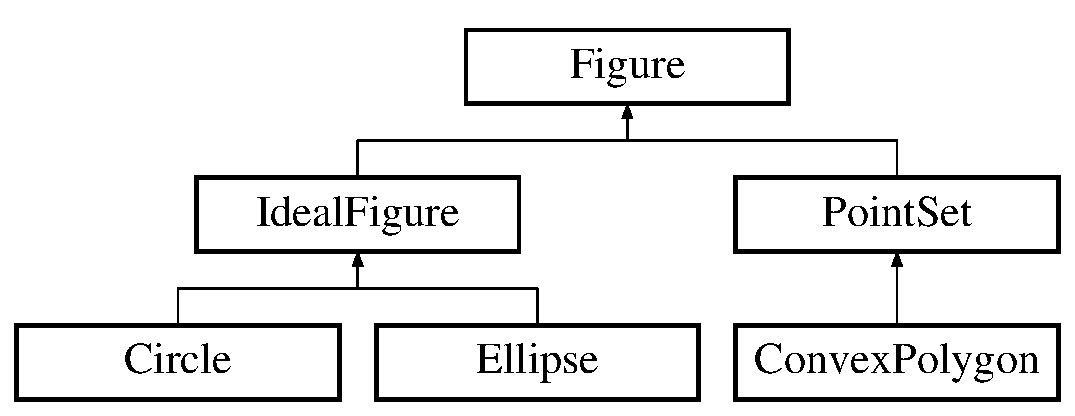
\includegraphics[height=3.000000cm]{class_figure}
\end{center}
\end{figure}
\subsection*{Public Member Functions}
\begin{DoxyCompactItemize}
\item 
virtual \hyperlink{class_figure_a654f8f4944edcfb248fb86b77b8b21d3}{$\sim$\+Figure} ()
\item 
virtual double \hyperlink{class_figure_a9860bda67fc9ce8127a812e167c4ce75}{area} ()=0
\item 
virtual double \hyperlink{class_figure_acae6802e2a55b322f7566f313d474546}{perimeter} ()=0
\item 
virtual \hyperlink{classtinyxml2_1_1_x_m_l_node}{tinyxml2\+::\+X\+M\+L\+Node} $\ast$ \hyperlink{class_figure_a11994f67ee209a46047e0897680f6313}{serialize} (\hyperlink{classtinyxml2_1_1_x_m_l_document}{tinyxml2\+::\+X\+M\+L\+Document} \&xml\+Doc)=0
\end{DoxyCompactItemize}


\subsection{Constructor \& Destructor Documentation}
\mbox{\Hypertarget{class_figure_a654f8f4944edcfb248fb86b77b8b21d3}\label{class_figure_a654f8f4944edcfb248fb86b77b8b21d3}} 
\index{Figure@{Figure}!````~Figure@{$\sim$\+Figure}}
\index{````~Figure@{$\sim$\+Figure}!Figure@{Figure}}
\subsubsection{\texorpdfstring{$\sim$\+Figure()}{~Figure()}}
{\footnotesize\ttfamily virtual Figure\+::$\sim$\+Figure (\begin{DoxyParamCaption}{ }\end{DoxyParamCaption})\hspace{0.3cm}{\ttfamily [inline]}, {\ttfamily [virtual]}}



\subsection{Member Function Documentation}
\mbox{\Hypertarget{class_figure_a9860bda67fc9ce8127a812e167c4ce75}\label{class_figure_a9860bda67fc9ce8127a812e167c4ce75}} 
\index{Figure@{Figure}!area@{area}}
\index{area@{area}!Figure@{Figure}}
\subsubsection{\texorpdfstring{area()}{area()}}
{\footnotesize\ttfamily virtual double Figure\+::area (\begin{DoxyParamCaption}{ }\end{DoxyParamCaption})\hspace{0.3cm}{\ttfamily [pure virtual]}}



Implemented in \hyperlink{class_point_set_aca8092b860a40743fb1c1189e8439764}{Point\+Set}, \hyperlink{class_ellipse_ad3de2759830df27c4ae1e65ecf46e7a1}{Ellipse}, \hyperlink{class_circle_a4f31d14f360b6e1f1acfb283ad65145a}{Circle}, and \hyperlink{class_convex_polygon_a4d8ca9c4d454308dcd95ae9f9dee2688}{Convex\+Polygon}.

\mbox{\Hypertarget{class_figure_acae6802e2a55b322f7566f313d474546}\label{class_figure_acae6802e2a55b322f7566f313d474546}} 
\index{Figure@{Figure}!perimeter@{perimeter}}
\index{perimeter@{perimeter}!Figure@{Figure}}
\subsubsection{\texorpdfstring{perimeter()}{perimeter()}}
{\footnotesize\ttfamily virtual double Figure\+::perimeter (\begin{DoxyParamCaption}{ }\end{DoxyParamCaption})\hspace{0.3cm}{\ttfamily [pure virtual]}}



Implemented in \hyperlink{class_point_set_a82b83d662bd5570e6e049e120e1c6bac}{Point\+Set}, \hyperlink{class_ellipse_a367ca002c3a95761d0b913f98bc4eb6e}{Ellipse}, \hyperlink{class_circle_ab0a4db4a814591918b0372feac5df46b}{Circle}, and \hyperlink{class_convex_polygon_ac8e11403c36adb4ac51b6c169257b605}{Convex\+Polygon}.

\mbox{\Hypertarget{class_figure_a11994f67ee209a46047e0897680f6313}\label{class_figure_a11994f67ee209a46047e0897680f6313}} 
\index{Figure@{Figure}!serialize@{serialize}}
\index{serialize@{serialize}!Figure@{Figure}}
\subsubsection{\texorpdfstring{serialize()}{serialize()}}
{\footnotesize\ttfamily virtual \hyperlink{classtinyxml2_1_1_x_m_l_node}{tinyxml2\+::\+X\+M\+L\+Node}$\ast$ Figure\+::serialize (\begin{DoxyParamCaption}\item[{\hyperlink{classtinyxml2_1_1_x_m_l_document}{tinyxml2\+::\+X\+M\+L\+Document} \&}]{xml\+Doc }\end{DoxyParamCaption})\hspace{0.3cm}{\ttfamily [pure virtual]}}



Implemented in \hyperlink{class_ellipse_ab6c64b8c54cb74a4552a5f4f487f8d7d}{Ellipse}, \hyperlink{class_ideal_figure_a5a795a3de8992af3fb9cee4a904b31a5}{Ideal\+Figure}, \hyperlink{class_circle_a86fa86f49342a310db5e717c75011487}{Circle}, \hyperlink{class_point_set_a282360046d7566f50d1ceec49aca0d89}{Point\+Set}, and \hyperlink{class_convex_polygon_ab7cfd51933dd7a3bf821056c292ca62c}{Convex\+Polygon}.



The documentation for this class was generated from the following file\+:\begin{DoxyCompactItemize}
\item 
\hyperlink{_figure_8h}{Figure.\+h}\end{DoxyCompactItemize}

\hypertarget{class_ideal_figure}{}\section{Ideal\+Figure Class Reference}
\label{class_ideal_figure}\index{Ideal\+Figure@{Ideal\+Figure}}


{\ttfamily \#include $<$Ideal\+Figure.\+h$>$}

Inheritance diagram for Ideal\+Figure\+:\begin{figure}[H]
\begin{center}
\leavevmode
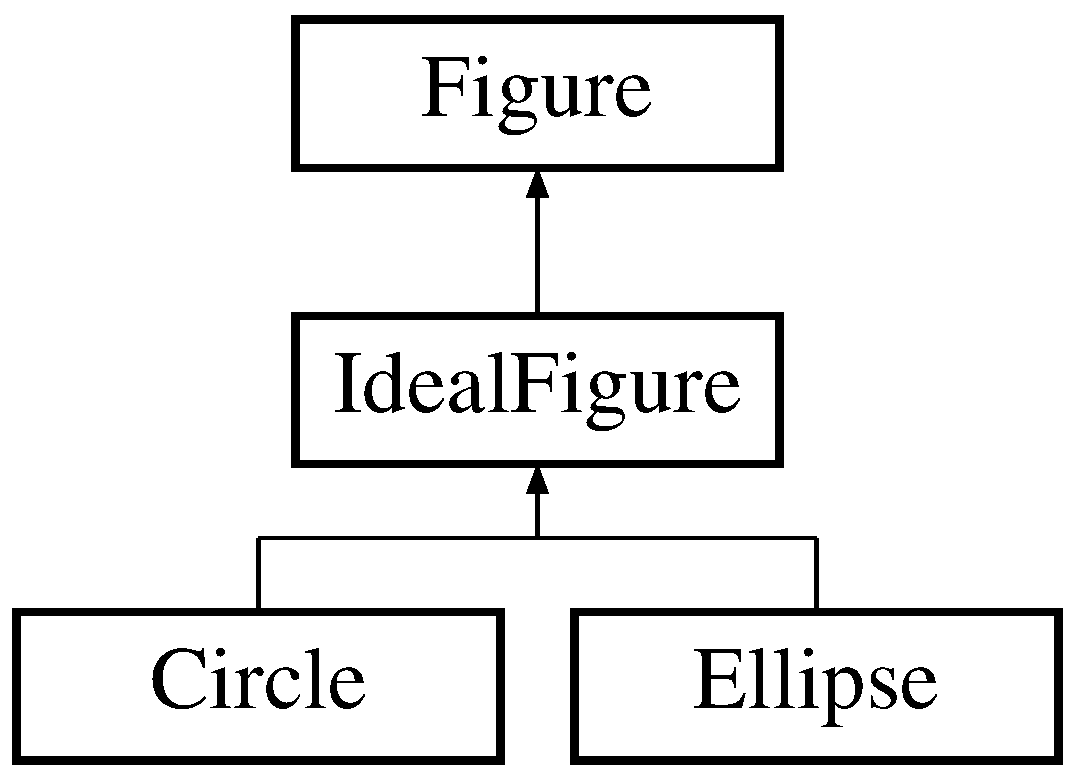
\includegraphics[height=3.000000cm]{class_ideal_figure}
\end{center}
\end{figure}
\subsection*{Public Member Functions}
\begin{DoxyCompactItemize}
\item 
\hyperlink{class_ideal_figure_a4df1554384722e84ffdd8c24e776b530}{Ideal\+Figure} (\hyperlink{class_point}{Point} origin=\hyperlink{class_point}{Point}(0, 0))
\item 
\hyperlink{class_ideal_figure_a35194b5caa4bec36ad18979cf9b33698}{Ideal\+Figure} (\hyperlink{class_point_a00b37528c0db634a12ecee9b29d79579}{Point\+::point\+Type} ox, \hyperlink{class_point_a00b37528c0db634a12ecee9b29d79579}{Point\+::point\+Type} oy)
\item 
\hyperlink{class_ideal_figure_a50b77911df4ac52c2aa65ab207e5a2db}{$\sim$\+Ideal\+Figure} ()
\item 
virtual \hyperlink{class_convex_polygon}{Convex\+Polygon} \hyperlink{class_ideal_figure_ae1b50ae419aa258fb7ebc7131e3d4a5d}{rasterize} (unsigned rezolution)=0
\item 
virtual \hyperlink{classtinyxml2_1_1_x_m_l_node}{tinyxml2\+::\+X\+M\+L\+Node} $\ast$ \hyperlink{class_ideal_figure_a5a795a3de8992af3fb9cee4a904b31a5}{serialize} (\hyperlink{classtinyxml2_1_1_x_m_l_document}{tinyxml2\+::\+X\+M\+L\+Document} \&xml\+Doc)
\end{DoxyCompactItemize}
\subsection*{Protected Attributes}
\begin{DoxyCompactItemize}
\item 
\hyperlink{class_point}{Point} \hyperlink{class_ideal_figure_a1d3d83b08736c67e93cf685ba5228814}{m\+\_\+origin}
\end{DoxyCompactItemize}


\subsection{Constructor \& Destructor Documentation}
\mbox{\Hypertarget{class_ideal_figure_a4df1554384722e84ffdd8c24e776b530}\label{class_ideal_figure_a4df1554384722e84ffdd8c24e776b530}} 
\index{Ideal\+Figure@{Ideal\+Figure}!Ideal\+Figure@{Ideal\+Figure}}
\index{Ideal\+Figure@{Ideal\+Figure}!Ideal\+Figure@{Ideal\+Figure}}
\subsubsection{\texorpdfstring{Ideal\+Figure()}{IdealFigure()}\hspace{0.1cm}{\footnotesize\ttfamily [1/2]}}
{\footnotesize\ttfamily Ideal\+Figure\+::\+Ideal\+Figure (\begin{DoxyParamCaption}\item[{\hyperlink{class_point}{Point}}]{origin = {\ttfamily \hyperlink{class_point}{Point}(0,~0)} }\end{DoxyParamCaption})\hspace{0.3cm}{\ttfamily [inline]}}

\mbox{\Hypertarget{class_ideal_figure_a35194b5caa4bec36ad18979cf9b33698}\label{class_ideal_figure_a35194b5caa4bec36ad18979cf9b33698}} 
\index{Ideal\+Figure@{Ideal\+Figure}!Ideal\+Figure@{Ideal\+Figure}}
\index{Ideal\+Figure@{Ideal\+Figure}!Ideal\+Figure@{Ideal\+Figure}}
\subsubsection{\texorpdfstring{Ideal\+Figure()}{IdealFigure()}\hspace{0.1cm}{\footnotesize\ttfamily [2/2]}}
{\footnotesize\ttfamily Ideal\+Figure\+::\+Ideal\+Figure (\begin{DoxyParamCaption}\item[{\hyperlink{class_point_a00b37528c0db634a12ecee9b29d79579}{Point\+::point\+Type}}]{ox,  }\item[{\hyperlink{class_point_a00b37528c0db634a12ecee9b29d79579}{Point\+::point\+Type}}]{oy }\end{DoxyParamCaption})\hspace{0.3cm}{\ttfamily [inline]}}

\mbox{\Hypertarget{class_ideal_figure_a50b77911df4ac52c2aa65ab207e5a2db}\label{class_ideal_figure_a50b77911df4ac52c2aa65ab207e5a2db}} 
\index{Ideal\+Figure@{Ideal\+Figure}!````~Ideal\+Figure@{$\sim$\+Ideal\+Figure}}
\index{````~Ideal\+Figure@{$\sim$\+Ideal\+Figure}!Ideal\+Figure@{Ideal\+Figure}}
\subsubsection{\texorpdfstring{$\sim$\+Ideal\+Figure()}{~IdealFigure()}}
{\footnotesize\ttfamily Ideal\+Figure\+::$\sim$\+Ideal\+Figure (\begin{DoxyParamCaption}{ }\end{DoxyParamCaption})\hspace{0.3cm}{\ttfamily [inline]}}



\subsection{Member Function Documentation}
\mbox{\Hypertarget{class_ideal_figure_ae1b50ae419aa258fb7ebc7131e3d4a5d}\label{class_ideal_figure_ae1b50ae419aa258fb7ebc7131e3d4a5d}} 
\index{Ideal\+Figure@{Ideal\+Figure}!rasterize@{rasterize}}
\index{rasterize@{rasterize}!Ideal\+Figure@{Ideal\+Figure}}
\subsubsection{\texorpdfstring{rasterize()}{rasterize()}}
{\footnotesize\ttfamily virtual \hyperlink{class_convex_polygon}{Convex\+Polygon} Ideal\+Figure\+::rasterize (\begin{DoxyParamCaption}\item[{unsigned}]{rezolution }\end{DoxyParamCaption})\hspace{0.3cm}{\ttfamily [pure virtual]}}

N\+O\+TE Functia nu pastreaza Aria/\+Perimetrul figurii dar este garantat ca va da tot timpul Un poligon convex inscris in figura data deci cu aria mai mica sau egala O valoare mai mare de 50 va da rezultate destul de bune dpdv vizual 

Implemented in \hyperlink{class_ellipse_a54a8e6dab13f9d3a0cc633101e2ce6d6}{Ellipse}, and \hyperlink{class_circle_ae5f140e34baceae51bb662bc15a5cecc}{Circle}.

\mbox{\Hypertarget{class_ideal_figure_a5a795a3de8992af3fb9cee4a904b31a5}\label{class_ideal_figure_a5a795a3de8992af3fb9cee4a904b31a5}} 
\index{Ideal\+Figure@{Ideal\+Figure}!serialize@{serialize}}
\index{serialize@{serialize}!Ideal\+Figure@{Ideal\+Figure}}
\subsubsection{\texorpdfstring{serialize()}{serialize()}}
{\footnotesize\ttfamily \hyperlink{classtinyxml2_1_1_x_m_l_node}{tinyxml2\+::\+X\+M\+L\+Node} $\ast$ Ideal\+Figure\+::serialize (\begin{DoxyParamCaption}\item[{\hyperlink{classtinyxml2_1_1_x_m_l_document}{tinyxml2\+::\+X\+M\+L\+Document} \&}]{xml\+Doc }\end{DoxyParamCaption})\hspace{0.3cm}{\ttfamily [virtual]}}



Implements \hyperlink{class_figure_a11994f67ee209a46047e0897680f6313}{Figure}.



Reimplemented in \hyperlink{class_ellipse_ab6c64b8c54cb74a4552a5f4f487f8d7d}{Ellipse}, and \hyperlink{class_circle_a86fa86f49342a310db5e717c75011487}{Circle}.



\subsection{Member Data Documentation}
\mbox{\Hypertarget{class_ideal_figure_a1d3d83b08736c67e93cf685ba5228814}\label{class_ideal_figure_a1d3d83b08736c67e93cf685ba5228814}} 
\index{Ideal\+Figure@{Ideal\+Figure}!m\+\_\+origin@{m\+\_\+origin}}
\index{m\+\_\+origin@{m\+\_\+origin}!Ideal\+Figure@{Ideal\+Figure}}
\subsubsection{\texorpdfstring{m\+\_\+origin}{m\_origin}}
{\footnotesize\ttfamily \hyperlink{class_point}{Point} Ideal\+Figure\+::m\+\_\+origin\hspace{0.3cm}{\ttfamily [protected]}}



The documentation for this class was generated from the following files\+:\begin{DoxyCompactItemize}
\item 
\hyperlink{_ideal_figure_8h}{Ideal\+Figure.\+h}\item 
\hyperlink{_ellipse_8cpp}{Ellipse.\+cpp}\end{DoxyCompactItemize}

\hypertarget{class_list}{}\section{List$<$ T $>$ Class Template Reference}
\label{class_list}\index{List$<$ T $>$@{List$<$ T $>$}}


{\ttfamily \#include $<$List.\+h$>$}

\subsection*{Classes}
\begin{DoxyCompactItemize}
\item 
struct \hyperlink{struct_list_1_1list_elem}{list\+Elem}
\end{DoxyCompactItemize}
\subsection*{Public Member Functions}
\begin{DoxyCompactItemize}
\item 
void \hyperlink{class_list_afea509b891b4541319974ea062e56d14}{insert} (T value)
\item 
bool \hyperlink{class_list_a6ae0df0d666cd7df1873106cdad93e2a}{is\+Empty} () const
\item 
\hyperlink{class_list_a5c5e27671b21b3815d4e25b953c69454}{List} ()
\item 
\hyperlink{class_list_a5ccfa2e417b814e6217a16696e4eab5d}{List} (const \hyperlink{class_list}{List}$<$ T $>$ \&l)
\item 
\hyperlink{class_list_a2b58189090f6e5ce52939c9195e59e85}{$\sim$\+List} ()
\item 
\hyperlink{class_list}{List}$<$ T $>$ $\ast$ \hyperlink{class_list_a93c7a3166ef42cc92e3df4c03cc92b2f}{operator=} (const \hyperlink{class_list}{List}$<$ T $>$ \&l)
\item 
T \hyperlink{class_list_abf3f18858335e6cebb451c80d22edf6f}{remove\+Head} ()
\begin{DoxyCompactList}\small\item\em Removes the first element of the list. \end{DoxyCompactList}\end{DoxyCompactItemize}
\subsection*{Protected Member Functions}
\begin{DoxyCompactItemize}
\item 
\hyperlink{struct_list_1_1list_elem}{list\+Elem} $\ast$ \hyperlink{class_list_a920e07d6f0047af1404e251a58adb4c2}{get\+Head} ()
\end{DoxyCompactItemize}
\subsection*{Friends}
\begin{DoxyCompactItemize}
\item 
class \hyperlink{class_list_a7719ee4382f1049bf06f7136702ca280}{Point\+Set}
\item 
class \hyperlink{class_list_a3efb5f47c0842087c3076652f3d62832}{Convex\+Polygon}
\end{DoxyCompactItemize}


\subsection{Constructor \& Destructor Documentation}
\mbox{\Hypertarget{class_list_a5c5e27671b21b3815d4e25b953c69454}\label{class_list_a5c5e27671b21b3815d4e25b953c69454}} 
\index{List@{List}!List@{List}}
\index{List@{List}!List@{List}}
\subsubsection{\texorpdfstring{List()}{List()}\hspace{0.1cm}{\footnotesize\ttfamily [1/2]}}
{\footnotesize\ttfamily template$<$class T$>$ \\
\hyperlink{class_list}{List}$<$ T $>$\+::\hyperlink{class_list}{List} (\begin{DoxyParamCaption}{ }\end{DoxyParamCaption})\hspace{0.3cm}{\ttfamily [inline]}}

\mbox{\Hypertarget{class_list_a5ccfa2e417b814e6217a16696e4eab5d}\label{class_list_a5ccfa2e417b814e6217a16696e4eab5d}} 
\index{List@{List}!List@{List}}
\index{List@{List}!List@{List}}
\subsubsection{\texorpdfstring{List()}{List()}\hspace{0.1cm}{\footnotesize\ttfamily [2/2]}}
{\footnotesize\ttfamily template$<$class T$>$ \\
\hyperlink{class_list}{List}$<$ T $>$\+::\hyperlink{class_list}{List} (\begin{DoxyParamCaption}\item[{const \hyperlink{class_list}{List}$<$ T $>$ \&}]{l }\end{DoxyParamCaption})\hspace{0.3cm}{\ttfamily [inline]}}

\mbox{\Hypertarget{class_list_a2b58189090f6e5ce52939c9195e59e85}\label{class_list_a2b58189090f6e5ce52939c9195e59e85}} 
\index{List@{List}!````~List@{$\sim$\+List}}
\index{````~List@{$\sim$\+List}!List@{List}}
\subsubsection{\texorpdfstring{$\sim$\+List()}{~List()}}
{\footnotesize\ttfamily template$<$class T$>$ \\
\hyperlink{class_list}{List}$<$ T $>$\+::$\sim$\hyperlink{class_list}{List} (\begin{DoxyParamCaption}{ }\end{DoxyParamCaption})\hspace{0.3cm}{\ttfamily [inline]}}



\subsection{Member Function Documentation}
\mbox{\Hypertarget{class_list_a920e07d6f0047af1404e251a58adb4c2}\label{class_list_a920e07d6f0047af1404e251a58adb4c2}} 
\index{List@{List}!get\+Head@{get\+Head}}
\index{get\+Head@{get\+Head}!List@{List}}
\subsubsection{\texorpdfstring{get\+Head()}{getHead()}}
{\footnotesize\ttfamily template$<$class T$>$ \\
\hyperlink{struct_list_1_1list_elem}{list\+Elem}$\ast$ \hyperlink{class_list}{List}$<$ T $>$\+::get\+Head (\begin{DoxyParamCaption}{ }\end{DoxyParamCaption})\hspace{0.3cm}{\ttfamily [inline]}, {\ttfamily [protected]}}

\mbox{\Hypertarget{class_list_afea509b891b4541319974ea062e56d14}\label{class_list_afea509b891b4541319974ea062e56d14}} 
\index{List@{List}!insert@{insert}}
\index{insert@{insert}!List@{List}}
\subsubsection{\texorpdfstring{insert()}{insert()}}
{\footnotesize\ttfamily template$<$class T$>$ \\
void \hyperlink{class_list}{List}$<$ T $>$\+::insert (\begin{DoxyParamCaption}\item[{T}]{value }\end{DoxyParamCaption})\hspace{0.3cm}{\ttfamily [inline]}}

\mbox{\Hypertarget{class_list_a6ae0df0d666cd7df1873106cdad93e2a}\label{class_list_a6ae0df0d666cd7df1873106cdad93e2a}} 
\index{List@{List}!is\+Empty@{is\+Empty}}
\index{is\+Empty@{is\+Empty}!List@{List}}
\subsubsection{\texorpdfstring{is\+Empty()}{isEmpty()}}
{\footnotesize\ttfamily template$<$class T$>$ \\
bool \hyperlink{class_list}{List}$<$ T $>$\+::is\+Empty (\begin{DoxyParamCaption}{ }\end{DoxyParamCaption}) const\hspace{0.3cm}{\ttfamily [inline]}}

\mbox{\Hypertarget{class_list_a93c7a3166ef42cc92e3df4c03cc92b2f}\label{class_list_a93c7a3166ef42cc92e3df4c03cc92b2f}} 
\index{List@{List}!operator=@{operator=}}
\index{operator=@{operator=}!List@{List}}
\subsubsection{\texorpdfstring{operator=()}{operator=()}}
{\footnotesize\ttfamily template$<$class T$>$ \\
\hyperlink{class_list}{List}$<$T$>$$\ast$ \hyperlink{class_list}{List}$<$ T $>$\+::operator= (\begin{DoxyParamCaption}\item[{const \hyperlink{class_list}{List}$<$ T $>$ \&}]{l }\end{DoxyParamCaption})\hspace{0.3cm}{\ttfamily [inline]}}

\mbox{\Hypertarget{class_list_abf3f18858335e6cebb451c80d22edf6f}\label{class_list_abf3f18858335e6cebb451c80d22edf6f}} 
\index{List@{List}!remove\+Head@{remove\+Head}}
\index{remove\+Head@{remove\+Head}!List@{List}}
\subsubsection{\texorpdfstring{remove\+Head()}{removeHead()}}
{\footnotesize\ttfamily template$<$class T$>$ \\
T \hyperlink{class_list}{List}$<$ T $>$\+::remove\+Head (\begin{DoxyParamCaption}{ }\end{DoxyParamCaption})\hspace{0.3cm}{\ttfamily [inline]}}



Removes the first element of the list. 



\subsection{Friends And Related Function Documentation}
\mbox{\Hypertarget{class_list_a3efb5f47c0842087c3076652f3d62832}\label{class_list_a3efb5f47c0842087c3076652f3d62832}} 
\index{List@{List}!Convex\+Polygon@{Convex\+Polygon}}
\index{Convex\+Polygon@{Convex\+Polygon}!List@{List}}
\subsubsection{\texorpdfstring{Convex\+Polygon}{ConvexPolygon}}
{\footnotesize\ttfamily template$<$class T$>$ \\
friend class \hyperlink{class_convex_polygon}{Convex\+Polygon}\hspace{0.3cm}{\ttfamily [friend]}}

\mbox{\Hypertarget{class_list_a7719ee4382f1049bf06f7136702ca280}\label{class_list_a7719ee4382f1049bf06f7136702ca280}} 
\index{List@{List}!Point\+Set@{Point\+Set}}
\index{Point\+Set@{Point\+Set}!List@{List}}
\subsubsection{\texorpdfstring{Point\+Set}{PointSet}}
{\footnotesize\ttfamily template$<$class T$>$ \\
friend class \hyperlink{class_point_set}{Point\+Set}\hspace{0.3cm}{\ttfamily [friend]}}



The documentation for this class was generated from the following file\+:\begin{DoxyCompactItemize}
\item 
\hyperlink{_list_8h}{List.\+h}\end{DoxyCompactItemize}

\hypertarget{struct_list_1_1list_elem}{}\section{List$<$ T $>$\+:\+:list\+Elem Struct Reference}
\label{struct_list_1_1list_elem}\index{List$<$ T $>$\+::list\+Elem@{List$<$ T $>$\+::list\+Elem}}


{\ttfamily \#include $<$List.\+h$>$}

\subsection*{Public Attributes}
\begin{DoxyCompactItemize}
\item 
T \hyperlink{struct_list_1_1list_elem_a12824c4d5a1d6d75edec6c1b8d08482f}{data}
\item 
\hyperlink{struct_list_1_1list_elem}{list\+Elem} $\ast$ \hyperlink{struct_list_1_1list_elem_adf3d9a3206aac09c39346270a6af223f}{next}
\end{DoxyCompactItemize}


\subsection{Member Data Documentation}
\mbox{\Hypertarget{struct_list_1_1list_elem_a12824c4d5a1d6d75edec6c1b8d08482f}\label{struct_list_1_1list_elem_a12824c4d5a1d6d75edec6c1b8d08482f}} 
\index{List\+::list\+Elem@{List\+::list\+Elem}!data@{data}}
\index{data@{data}!List\+::list\+Elem@{List\+::list\+Elem}}
\subsubsection{\texorpdfstring{data}{data}}
{\footnotesize\ttfamily template$<$class T$>$ \\
T \hyperlink{class_list}{List}$<$ T $>$\+::list\+Elem\+::data}

\mbox{\Hypertarget{struct_list_1_1list_elem_adf3d9a3206aac09c39346270a6af223f}\label{struct_list_1_1list_elem_adf3d9a3206aac09c39346270a6af223f}} 
\index{List\+::list\+Elem@{List\+::list\+Elem}!next@{next}}
\index{next@{next}!List\+::list\+Elem@{List\+::list\+Elem}}
\subsubsection{\texorpdfstring{next}{next}}
{\footnotesize\ttfamily template$<$class T$>$ \\
\hyperlink{struct_list_1_1list_elem}{list\+Elem}$\ast$ \hyperlink{class_list}{List}$<$ T $>$\+::list\+Elem\+::next}



The documentation for this struct was generated from the following file\+:\begin{DoxyCompactItemize}
\item 
\hyperlink{_list_8h}{List.\+h}\end{DoxyCompactItemize}

\hypertarget{structtinyxml2_1_1_long_fits_into_size_t_minus_one}{}\section{tinyxml2\+:\+:Long\+Fits\+Into\+Size\+T\+Minus\+One$<$ bool $>$ Struct Template Reference}
\label{structtinyxml2_1_1_long_fits_into_size_t_minus_one}\index{tinyxml2\+::\+Long\+Fits\+Into\+Size\+T\+Minus\+One$<$ bool $>$@{tinyxml2\+::\+Long\+Fits\+Into\+Size\+T\+Minus\+One$<$ bool $>$}}
\subsection*{Static Public Member Functions}
\begin{DoxyCompactItemize}
\item 
static bool \hyperlink{structtinyxml2_1_1_long_fits_into_size_t_minus_one_a3057710104ab733963eb32fda0bc374c}{Fits} (unsigned long value)
\end{DoxyCompactItemize}


\subsection{Member Function Documentation}
\mbox{\Hypertarget{structtinyxml2_1_1_long_fits_into_size_t_minus_one_a3057710104ab733963eb32fda0bc374c}\label{structtinyxml2_1_1_long_fits_into_size_t_minus_one_a3057710104ab733963eb32fda0bc374c}} 
\index{tinyxml2\+::\+Long\+Fits\+Into\+Size\+T\+Minus\+One@{tinyxml2\+::\+Long\+Fits\+Into\+Size\+T\+Minus\+One}!Fits@{Fits}}
\index{Fits@{Fits}!tinyxml2\+::\+Long\+Fits\+Into\+Size\+T\+Minus\+One@{tinyxml2\+::\+Long\+Fits\+Into\+Size\+T\+Minus\+One}}
\subsubsection{\texorpdfstring{Fits()}{Fits()}}
{\footnotesize\ttfamily template$<$bool  = (sizeof(unsigned long) $>$= sizeof(size\+\_\+t))$>$ \\
static bool \hyperlink{structtinyxml2_1_1_long_fits_into_size_t_minus_one}{tinyxml2\+::\+Long\+Fits\+Into\+Size\+T\+Minus\+One}$<$ bool $>$\+::Fits (\begin{DoxyParamCaption}\item[{unsigned long}]{value }\end{DoxyParamCaption})\hspace{0.3cm}{\ttfamily [inline]}, {\ttfamily [static]}}



The documentation for this struct was generated from the following file\+:\begin{DoxyCompactItemize}
\item 
\hyperlink{tinyxml2_8cpp}{tinyxml2.\+cpp}\end{DoxyCompactItemize}

\hypertarget{structtinyxml2_1_1_long_fits_into_size_t_minus_one_3_01false_01_4}{}\section{tinyxml2\+:\+:Long\+Fits\+Into\+Size\+T\+Minus\+One$<$ false $>$ Struct Template Reference}
\label{structtinyxml2_1_1_long_fits_into_size_t_minus_one_3_01false_01_4}\index{tinyxml2\+::\+Long\+Fits\+Into\+Size\+T\+Minus\+One$<$ false $>$@{tinyxml2\+::\+Long\+Fits\+Into\+Size\+T\+Minus\+One$<$ false $>$}}
\subsection*{Static Public Member Functions}
\begin{DoxyCompactItemize}
\item 
static bool \hyperlink{structtinyxml2_1_1_long_fits_into_size_t_minus_one_3_01false_01_4_a29b01087f38a951276df69d358dc0764}{Fits} (unsigned long)
\end{DoxyCompactItemize}


\subsection{Member Function Documentation}
\mbox{\Hypertarget{structtinyxml2_1_1_long_fits_into_size_t_minus_one_3_01false_01_4_a29b01087f38a951276df69d358dc0764}\label{structtinyxml2_1_1_long_fits_into_size_t_minus_one_3_01false_01_4_a29b01087f38a951276df69d358dc0764}} 
\index{tinyxml2\+::\+Long\+Fits\+Into\+Size\+T\+Minus\+One$<$ false $>$@{tinyxml2\+::\+Long\+Fits\+Into\+Size\+T\+Minus\+One$<$ false $>$}!Fits@{Fits}}
\index{Fits@{Fits}!tinyxml2\+::\+Long\+Fits\+Into\+Size\+T\+Minus\+One$<$ false $>$@{tinyxml2\+::\+Long\+Fits\+Into\+Size\+T\+Minus\+One$<$ false $>$}}
\subsubsection{\texorpdfstring{Fits()}{Fits()}}
{\footnotesize\ttfamily static bool \hyperlink{structtinyxml2_1_1_long_fits_into_size_t_minus_one}{tinyxml2\+::\+Long\+Fits\+Into\+Size\+T\+Minus\+One}$<$ false $>$\+::Fits (\begin{DoxyParamCaption}\item[{unsigned}]{long }\end{DoxyParamCaption})\hspace{0.3cm}{\ttfamily [inline]}, {\ttfamily [static]}}



The documentation for this struct was generated from the following file\+:\begin{DoxyCompactItemize}
\item 
\hyperlink{tinyxml2_8cpp}{tinyxml2.\+cpp}\end{DoxyCompactItemize}

\hypertarget{classtinyxml2_1_1_mem_pool}{}\section{tinyxml2\+:\+:Mem\+Pool Class Reference}
\label{classtinyxml2_1_1_mem_pool}\index{tinyxml2\+::\+Mem\+Pool@{tinyxml2\+::\+Mem\+Pool}}


{\ttfamily \#include $<$tinyxml2.\+h$>$}

Inheritance diagram for tinyxml2\+:\+:Mem\+Pool\+:\begin{figure}[H]
\begin{center}
\leavevmode
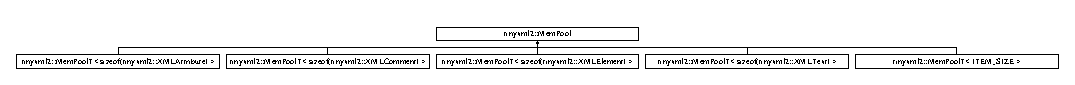
\includegraphics[height=0.691358cm]{classtinyxml2_1_1_mem_pool}
\end{center}
\end{figure}
\subsection*{Public Member Functions}
\begin{DoxyCompactItemize}
\item 
\hyperlink{classtinyxml2_1_1_mem_pool_a9101a0083d7370c85bd5aaaba7157f84}{Mem\+Pool} ()
\item 
virtual \hyperlink{classtinyxml2_1_1_mem_pool_ae55ad9e3faeca702e6ccbb38fdbcad72}{$\sim$\+Mem\+Pool} ()
\item 
virtual int \hyperlink{classtinyxml2_1_1_mem_pool_a0c518d49e3a94bde566f61e13b7240bb}{Item\+Size} () const =0
\item 
virtual void $\ast$ \hyperlink{classtinyxml2_1_1_mem_pool_a4f977b5fed752c0bbfe5295f469d6449}{Alloc} ()=0
\item 
virtual void \hyperlink{classtinyxml2_1_1_mem_pool_a49e3bfac2cba2ebd6776b31e571f64f7}{Free} (void $\ast$)=0
\item 
virtual void \hyperlink{classtinyxml2_1_1_mem_pool_ac5804dd1387b2e4de5eef710076a0db1}{Set\+Tracked} ()=0
\item 
virtual void \hyperlink{classtinyxml2_1_1_mem_pool_a74fcdef9756917c8ae19fbbb4d658ed7}{Clear} ()=0
\end{DoxyCompactItemize}


\subsection{Constructor \& Destructor Documentation}
\mbox{\Hypertarget{classtinyxml2_1_1_mem_pool_a9101a0083d7370c85bd5aaaba7157f84}\label{classtinyxml2_1_1_mem_pool_a9101a0083d7370c85bd5aaaba7157f84}} 
\index{tinyxml2\+::\+Mem\+Pool@{tinyxml2\+::\+Mem\+Pool}!Mem\+Pool@{Mem\+Pool}}
\index{Mem\+Pool@{Mem\+Pool}!tinyxml2\+::\+Mem\+Pool@{tinyxml2\+::\+Mem\+Pool}}
\subsubsection{\texorpdfstring{Mem\+Pool()}{MemPool()}}
{\footnotesize\ttfamily tinyxml2\+::\+Mem\+Pool\+::\+Mem\+Pool (\begin{DoxyParamCaption}{ }\end{DoxyParamCaption})\hspace{0.3cm}{\ttfamily [inline]}}

\mbox{\Hypertarget{classtinyxml2_1_1_mem_pool_ae55ad9e3faeca702e6ccbb38fdbcad72}\label{classtinyxml2_1_1_mem_pool_ae55ad9e3faeca702e6ccbb38fdbcad72}} 
\index{tinyxml2\+::\+Mem\+Pool@{tinyxml2\+::\+Mem\+Pool}!````~Mem\+Pool@{$\sim$\+Mem\+Pool}}
\index{````~Mem\+Pool@{$\sim$\+Mem\+Pool}!tinyxml2\+::\+Mem\+Pool@{tinyxml2\+::\+Mem\+Pool}}
\subsubsection{\texorpdfstring{$\sim$\+Mem\+Pool()}{~MemPool()}}
{\footnotesize\ttfamily virtual tinyxml2\+::\+Mem\+Pool\+::$\sim$\+Mem\+Pool (\begin{DoxyParamCaption}{ }\end{DoxyParamCaption})\hspace{0.3cm}{\ttfamily [inline]}, {\ttfamily [virtual]}}



\subsection{Member Function Documentation}
\mbox{\Hypertarget{classtinyxml2_1_1_mem_pool_a4f977b5fed752c0bbfe5295f469d6449}\label{classtinyxml2_1_1_mem_pool_a4f977b5fed752c0bbfe5295f469d6449}} 
\index{tinyxml2\+::\+Mem\+Pool@{tinyxml2\+::\+Mem\+Pool}!Alloc@{Alloc}}
\index{Alloc@{Alloc}!tinyxml2\+::\+Mem\+Pool@{tinyxml2\+::\+Mem\+Pool}}
\subsubsection{\texorpdfstring{Alloc()}{Alloc()}}
{\footnotesize\ttfamily virtual void$\ast$ tinyxml2\+::\+Mem\+Pool\+::\+Alloc (\begin{DoxyParamCaption}{ }\end{DoxyParamCaption})\hspace{0.3cm}{\ttfamily [pure virtual]}}



Implemented in \hyperlink{classtinyxml2_1_1_mem_pool_t_a810fd2b0caf56b8b688e55f2768f96c7}{tinyxml2\+::\+Mem\+Pool\+T$<$ I\+T\+E\+M\+\_\+\+S\+I\+Z\+E $>$}, \hyperlink{classtinyxml2_1_1_mem_pool_t_a810fd2b0caf56b8b688e55f2768f96c7}{tinyxml2\+::\+Mem\+Pool\+T$<$ sizeof(tinyxml2\+::\+X\+M\+L\+Comment) $>$}, \hyperlink{classtinyxml2_1_1_mem_pool_t_a810fd2b0caf56b8b688e55f2768f96c7}{tinyxml2\+::\+Mem\+Pool\+T$<$ sizeof(tinyxml2\+::\+X\+M\+L\+Text) $>$}, \hyperlink{classtinyxml2_1_1_mem_pool_t_a810fd2b0caf56b8b688e55f2768f96c7}{tinyxml2\+::\+Mem\+Pool\+T$<$ sizeof(tinyxml2\+::\+X\+M\+L\+Attribute) $>$}, and \hyperlink{classtinyxml2_1_1_mem_pool_t_a810fd2b0caf56b8b688e55f2768f96c7}{tinyxml2\+::\+Mem\+Pool\+T$<$ sizeof(tinyxml2\+::\+X\+M\+L\+Element) $>$}.

\mbox{\Hypertarget{classtinyxml2_1_1_mem_pool_a74fcdef9756917c8ae19fbbb4d658ed7}\label{classtinyxml2_1_1_mem_pool_a74fcdef9756917c8ae19fbbb4d658ed7}} 
\index{tinyxml2\+::\+Mem\+Pool@{tinyxml2\+::\+Mem\+Pool}!Clear@{Clear}}
\index{Clear@{Clear}!tinyxml2\+::\+Mem\+Pool@{tinyxml2\+::\+Mem\+Pool}}
\subsubsection{\texorpdfstring{Clear()}{Clear()}}
{\footnotesize\ttfamily virtual void tinyxml2\+::\+Mem\+Pool\+::\+Clear (\begin{DoxyParamCaption}{ }\end{DoxyParamCaption})\hspace{0.3cm}{\ttfamily [pure virtual]}}



Implemented in \hyperlink{classtinyxml2_1_1_mem_pool_t_a22d595caa0e9d23aa080f49ca6475fdd}{tinyxml2\+::\+Mem\+Pool\+T$<$ I\+T\+E\+M\+\_\+\+S\+I\+Z\+E $>$}, \hyperlink{classtinyxml2_1_1_mem_pool_t_a22d595caa0e9d23aa080f49ca6475fdd}{tinyxml2\+::\+Mem\+Pool\+T$<$ sizeof(tinyxml2\+::\+X\+M\+L\+Comment) $>$}, \hyperlink{classtinyxml2_1_1_mem_pool_t_a22d595caa0e9d23aa080f49ca6475fdd}{tinyxml2\+::\+Mem\+Pool\+T$<$ sizeof(tinyxml2\+::\+X\+M\+L\+Text) $>$}, \hyperlink{classtinyxml2_1_1_mem_pool_t_a22d595caa0e9d23aa080f49ca6475fdd}{tinyxml2\+::\+Mem\+Pool\+T$<$ sizeof(tinyxml2\+::\+X\+M\+L\+Attribute) $>$}, and \hyperlink{classtinyxml2_1_1_mem_pool_t_a22d595caa0e9d23aa080f49ca6475fdd}{tinyxml2\+::\+Mem\+Pool\+T$<$ sizeof(tinyxml2\+::\+X\+M\+L\+Element) $>$}.

\mbox{\Hypertarget{classtinyxml2_1_1_mem_pool_a49e3bfac2cba2ebd6776b31e571f64f7}\label{classtinyxml2_1_1_mem_pool_a49e3bfac2cba2ebd6776b31e571f64f7}} 
\index{tinyxml2\+::\+Mem\+Pool@{tinyxml2\+::\+Mem\+Pool}!Free@{Free}}
\index{Free@{Free}!tinyxml2\+::\+Mem\+Pool@{tinyxml2\+::\+Mem\+Pool}}
\subsubsection{\texorpdfstring{Free()}{Free()}}
{\footnotesize\ttfamily virtual void tinyxml2\+::\+Mem\+Pool\+::\+Free (\begin{DoxyParamCaption}\item[{void $\ast$}]{ }\end{DoxyParamCaption})\hspace{0.3cm}{\ttfamily [pure virtual]}}



Implemented in \hyperlink{classtinyxml2_1_1_mem_pool_t_a408ce0918e9d3d5e5e1cc4896944875f}{tinyxml2\+::\+Mem\+Pool\+T$<$ I\+T\+E\+M\+\_\+\+S\+I\+Z\+E $>$}, \hyperlink{classtinyxml2_1_1_mem_pool_t_a408ce0918e9d3d5e5e1cc4896944875f}{tinyxml2\+::\+Mem\+Pool\+T$<$ sizeof(tinyxml2\+::\+X\+M\+L\+Comment) $>$}, \hyperlink{classtinyxml2_1_1_mem_pool_t_a408ce0918e9d3d5e5e1cc4896944875f}{tinyxml2\+::\+Mem\+Pool\+T$<$ sizeof(tinyxml2\+::\+X\+M\+L\+Text) $>$}, \hyperlink{classtinyxml2_1_1_mem_pool_t_a408ce0918e9d3d5e5e1cc4896944875f}{tinyxml2\+::\+Mem\+Pool\+T$<$ sizeof(tinyxml2\+::\+X\+M\+L\+Attribute) $>$}, and \hyperlink{classtinyxml2_1_1_mem_pool_t_a408ce0918e9d3d5e5e1cc4896944875f}{tinyxml2\+::\+Mem\+Pool\+T$<$ sizeof(tinyxml2\+::\+X\+M\+L\+Element) $>$}.

\mbox{\Hypertarget{classtinyxml2_1_1_mem_pool_a0c518d49e3a94bde566f61e13b7240bb}\label{classtinyxml2_1_1_mem_pool_a0c518d49e3a94bde566f61e13b7240bb}} 
\index{tinyxml2\+::\+Mem\+Pool@{tinyxml2\+::\+Mem\+Pool}!Item\+Size@{Item\+Size}}
\index{Item\+Size@{Item\+Size}!tinyxml2\+::\+Mem\+Pool@{tinyxml2\+::\+Mem\+Pool}}
\subsubsection{\texorpdfstring{Item\+Size()}{ItemSize()}}
{\footnotesize\ttfamily virtual int tinyxml2\+::\+Mem\+Pool\+::\+Item\+Size (\begin{DoxyParamCaption}{ }\end{DoxyParamCaption}) const\hspace{0.3cm}{\ttfamily [pure virtual]}}



Implemented in \hyperlink{classtinyxml2_1_1_mem_pool_t_a54e4d9b343459ef1731314a99877ff35}{tinyxml2\+::\+Mem\+Pool\+T$<$ I\+T\+E\+M\+\_\+\+S\+I\+Z\+E $>$}, \hyperlink{classtinyxml2_1_1_mem_pool_t_a54e4d9b343459ef1731314a99877ff35}{tinyxml2\+::\+Mem\+Pool\+T$<$ sizeof(tinyxml2\+::\+X\+M\+L\+Comment) $>$}, \hyperlink{classtinyxml2_1_1_mem_pool_t_a54e4d9b343459ef1731314a99877ff35}{tinyxml2\+::\+Mem\+Pool\+T$<$ sizeof(tinyxml2\+::\+X\+M\+L\+Text) $>$}, \hyperlink{classtinyxml2_1_1_mem_pool_t_a54e4d9b343459ef1731314a99877ff35}{tinyxml2\+::\+Mem\+Pool\+T$<$ sizeof(tinyxml2\+::\+X\+M\+L\+Attribute) $>$}, and \hyperlink{classtinyxml2_1_1_mem_pool_t_a54e4d9b343459ef1731314a99877ff35}{tinyxml2\+::\+Mem\+Pool\+T$<$ sizeof(tinyxml2\+::\+X\+M\+L\+Element) $>$}.

\mbox{\Hypertarget{classtinyxml2_1_1_mem_pool_ac5804dd1387b2e4de5eef710076a0db1}\label{classtinyxml2_1_1_mem_pool_ac5804dd1387b2e4de5eef710076a0db1}} 
\index{tinyxml2\+::\+Mem\+Pool@{tinyxml2\+::\+Mem\+Pool}!Set\+Tracked@{Set\+Tracked}}
\index{Set\+Tracked@{Set\+Tracked}!tinyxml2\+::\+Mem\+Pool@{tinyxml2\+::\+Mem\+Pool}}
\subsubsection{\texorpdfstring{Set\+Tracked()}{SetTracked()}}
{\footnotesize\ttfamily virtual void tinyxml2\+::\+Mem\+Pool\+::\+Set\+Tracked (\begin{DoxyParamCaption}{ }\end{DoxyParamCaption})\hspace{0.3cm}{\ttfamily [pure virtual]}}



Implemented in \hyperlink{classtinyxml2_1_1_mem_pool_t_aee3c611215ae08cce41a940bf2763027}{tinyxml2\+::\+Mem\+Pool\+T$<$ I\+T\+E\+M\+\_\+\+S\+I\+Z\+E $>$}, \hyperlink{classtinyxml2_1_1_mem_pool_t_aee3c611215ae08cce41a940bf2763027}{tinyxml2\+::\+Mem\+Pool\+T$<$ sizeof(tinyxml2\+::\+X\+M\+L\+Comment) $>$}, \hyperlink{classtinyxml2_1_1_mem_pool_t_aee3c611215ae08cce41a940bf2763027}{tinyxml2\+::\+Mem\+Pool\+T$<$ sizeof(tinyxml2\+::\+X\+M\+L\+Text) $>$}, \hyperlink{classtinyxml2_1_1_mem_pool_t_aee3c611215ae08cce41a940bf2763027}{tinyxml2\+::\+Mem\+Pool\+T$<$ sizeof(tinyxml2\+::\+X\+M\+L\+Attribute) $>$}, and \hyperlink{classtinyxml2_1_1_mem_pool_t_aee3c611215ae08cce41a940bf2763027}{tinyxml2\+::\+Mem\+Pool\+T$<$ sizeof(tinyxml2\+::\+X\+M\+L\+Element) $>$}.



The documentation for this class was generated from the following file\+:\begin{DoxyCompactItemize}
\item 
\hyperlink{tinyxml2_8h}{tinyxml2.\+h}\end{DoxyCompactItemize}

\hypertarget{classtinyxml2_1_1_mem_pool_t}{}\section{tinyxml2\+:\+:Mem\+PoolT$<$ I\+T\+E\+M\+\_\+\+S\+I\+ZE $>$ Class Template Reference}
\label{classtinyxml2_1_1_mem_pool_t}\index{tinyxml2\+::\+Mem\+Pool\+T$<$ I\+T\+E\+M\+\_\+\+S\+I\+Z\+E $>$@{tinyxml2\+::\+Mem\+Pool\+T$<$ I\+T\+E\+M\+\_\+\+S\+I\+Z\+E $>$}}


{\ttfamily \#include $<$tinyxml2.\+h$>$}

Inheritance diagram for tinyxml2\+:\+:Mem\+PoolT$<$ I\+T\+E\+M\+\_\+\+S\+I\+ZE $>$\+:\begin{figure}[H]
\begin{center}
\leavevmode
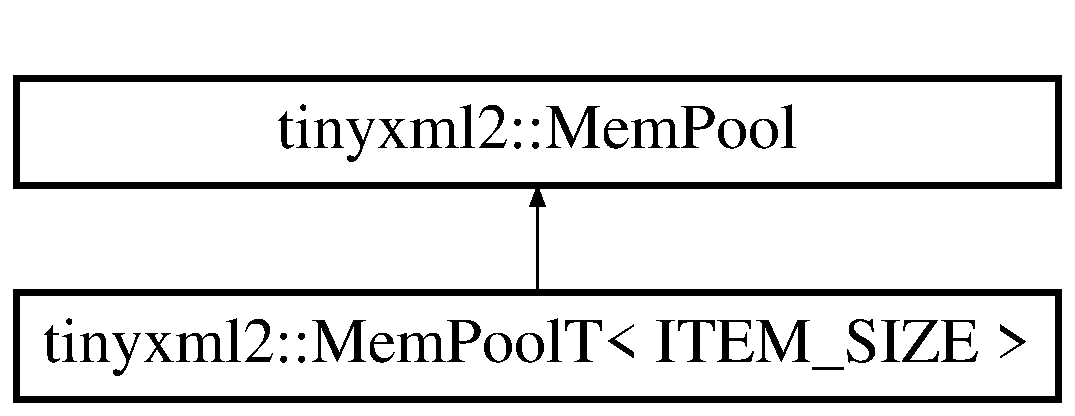
\includegraphics[height=2.000000cm]{classtinyxml2_1_1_mem_pool_t}
\end{center}
\end{figure}
\subsection*{Public Types}
\begin{DoxyCompactItemize}
\item 
enum \{ \hyperlink{classtinyxml2_1_1_mem_pool_t_a04cf45156e6f913f93972869ff8a1d94ab72c1e16d6626854c41feb19e60c54d1}{I\+T\+E\+M\+S\+\_\+\+P\+E\+R\+\_\+\+B\+L\+O\+CK} = (4 $\ast$ 1024) / I\+T\+E\+M\+\_\+\+S\+I\+ZE
 \}
\end{DoxyCompactItemize}
\subsection*{Public Member Functions}
\begin{DoxyCompactItemize}
\item 
\hyperlink{classtinyxml2_1_1_mem_pool_t_ac8fa6dbb403f009cf9c8a33c6f2803b3}{Mem\+PoolT} ()
\item 
\hyperlink{classtinyxml2_1_1_mem_pool_t_a5fa4fee934a3df2b9e74282244d78390}{$\sim$\+Mem\+PoolT} ()
\item 
void \hyperlink{classtinyxml2_1_1_mem_pool_t_a22d595caa0e9d23aa080f49ca6475fdd}{Clear} ()
\item 
virtual int \hyperlink{classtinyxml2_1_1_mem_pool_t_a54e4d9b343459ef1731314a99877ff35}{Item\+Size} () const
\item 
int \hyperlink{classtinyxml2_1_1_mem_pool_t_a445a6c80151ba6268b24ec62a7c84d74}{Current\+Allocs} () const
\item 
virtual void $\ast$ \hyperlink{classtinyxml2_1_1_mem_pool_t_a810fd2b0caf56b8b688e55f2768f96c7}{Alloc} ()
\item 
virtual void \hyperlink{classtinyxml2_1_1_mem_pool_t_a408ce0918e9d3d5e5e1cc4896944875f}{Free} (void $\ast$mem)
\item 
void \hyperlink{classtinyxml2_1_1_mem_pool_t_a47eefbd934ef70d973ea41d41ab5f239}{Trace} (const char $\ast$name)
\item 
void \hyperlink{classtinyxml2_1_1_mem_pool_t_aee3c611215ae08cce41a940bf2763027}{Set\+Tracked} ()
\item 
int \hyperlink{classtinyxml2_1_1_mem_pool_t_a3bcdc302ae15d2810e11192321a8f5f1}{Untracked} () const
\end{DoxyCompactItemize}


\subsection{Member Enumeration Documentation}
\mbox{\Hypertarget{classtinyxml2_1_1_mem_pool_t_a04cf45156e6f913f93972869ff8a1d94}\label{classtinyxml2_1_1_mem_pool_t_a04cf45156e6f913f93972869ff8a1d94}} 
\subsubsection{\texorpdfstring{anonymous enum}{anonymous enum}}
{\footnotesize\ttfamily template$<$int I\+T\+E\+M\+\_\+\+S\+I\+ZE$>$ \\
anonymous enum}

\begin{DoxyEnumFields}{Enumerator}
\raisebox{\heightof{T}}[0pt][0pt]{\index{I\+T\+E\+M\+S\+\_\+\+P\+E\+R\+\_\+\+B\+L\+O\+CK@{I\+T\+E\+M\+S\+\_\+\+P\+E\+R\+\_\+\+B\+L\+O\+CK}!tinyxml2\+::\+Mem\+PoolT@{tinyxml2\+::\+Mem\+PoolT}}\index{tinyxml2\+::\+Mem\+PoolT@{tinyxml2\+::\+Mem\+PoolT}!I\+T\+E\+M\+S\+\_\+\+P\+E\+R\+\_\+\+B\+L\+O\+CK@{I\+T\+E\+M\+S\+\_\+\+P\+E\+R\+\_\+\+B\+L\+O\+CK}}}\mbox{\Hypertarget{classtinyxml2_1_1_mem_pool_t_a04cf45156e6f913f93972869ff8a1d94ab72c1e16d6626854c41feb19e60c54d1}\label{classtinyxml2_1_1_mem_pool_t_a04cf45156e6f913f93972869ff8a1d94ab72c1e16d6626854c41feb19e60c54d1}} 
I\+T\+E\+M\+S\+\_\+\+P\+E\+R\+\_\+\+B\+L\+O\+CK&\\
\hline

\end{DoxyEnumFields}


\subsection{Constructor \& Destructor Documentation}
\mbox{\Hypertarget{classtinyxml2_1_1_mem_pool_t_ac8fa6dbb403f009cf9c8a33c6f2803b3}\label{classtinyxml2_1_1_mem_pool_t_ac8fa6dbb403f009cf9c8a33c6f2803b3}} 
\index{tinyxml2\+::\+Mem\+PoolT@{tinyxml2\+::\+Mem\+PoolT}!Mem\+PoolT@{Mem\+PoolT}}
\index{Mem\+PoolT@{Mem\+PoolT}!tinyxml2\+::\+Mem\+PoolT@{tinyxml2\+::\+Mem\+PoolT}}
\subsubsection{\texorpdfstring{Mem\+Pool\+T()}{MemPoolT()}}
{\footnotesize\ttfamily template$<$int I\+T\+E\+M\+\_\+\+S\+I\+ZE$>$ \\
\hyperlink{classtinyxml2_1_1_mem_pool_t}{tinyxml2\+::\+Mem\+PoolT}$<$ I\+T\+E\+M\+\_\+\+S\+I\+ZE $>$\+::\hyperlink{classtinyxml2_1_1_mem_pool_t}{Mem\+PoolT} (\begin{DoxyParamCaption}{ }\end{DoxyParamCaption})\hspace{0.3cm}{\ttfamily [inline]}}

\mbox{\Hypertarget{classtinyxml2_1_1_mem_pool_t_a5fa4fee934a3df2b9e74282244d78390}\label{classtinyxml2_1_1_mem_pool_t_a5fa4fee934a3df2b9e74282244d78390}} 
\index{tinyxml2\+::\+Mem\+PoolT@{tinyxml2\+::\+Mem\+PoolT}!````~Mem\+PoolT@{$\sim$\+Mem\+PoolT}}
\index{````~Mem\+PoolT@{$\sim$\+Mem\+PoolT}!tinyxml2\+::\+Mem\+PoolT@{tinyxml2\+::\+Mem\+PoolT}}
\subsubsection{\texorpdfstring{$\sim$\+Mem\+Pool\+T()}{~MemPoolT()}}
{\footnotesize\ttfamily template$<$int I\+T\+E\+M\+\_\+\+S\+I\+ZE$>$ \\
\hyperlink{classtinyxml2_1_1_mem_pool_t}{tinyxml2\+::\+Mem\+PoolT}$<$ I\+T\+E\+M\+\_\+\+S\+I\+ZE $>$\+::$\sim$\hyperlink{classtinyxml2_1_1_mem_pool_t}{Mem\+PoolT} (\begin{DoxyParamCaption}{ }\end{DoxyParamCaption})\hspace{0.3cm}{\ttfamily [inline]}}



\subsection{Member Function Documentation}
\mbox{\Hypertarget{classtinyxml2_1_1_mem_pool_t_a810fd2b0caf56b8b688e55f2768f96c7}\label{classtinyxml2_1_1_mem_pool_t_a810fd2b0caf56b8b688e55f2768f96c7}} 
\index{tinyxml2\+::\+Mem\+PoolT@{tinyxml2\+::\+Mem\+PoolT}!Alloc@{Alloc}}
\index{Alloc@{Alloc}!tinyxml2\+::\+Mem\+PoolT@{tinyxml2\+::\+Mem\+PoolT}}
\subsubsection{\texorpdfstring{Alloc()}{Alloc()}}
{\footnotesize\ttfamily template$<$int I\+T\+E\+M\+\_\+\+S\+I\+ZE$>$ \\
virtual void$\ast$ \hyperlink{classtinyxml2_1_1_mem_pool_t}{tinyxml2\+::\+Mem\+PoolT}$<$ I\+T\+E\+M\+\_\+\+S\+I\+ZE $>$\+::Alloc (\begin{DoxyParamCaption}{ }\end{DoxyParamCaption})\hspace{0.3cm}{\ttfamily [inline]}, {\ttfamily [virtual]}}



Implements \hyperlink{classtinyxml2_1_1_mem_pool_a4f977b5fed752c0bbfe5295f469d6449}{tinyxml2\+::\+Mem\+Pool}.

\mbox{\Hypertarget{classtinyxml2_1_1_mem_pool_t_a22d595caa0e9d23aa080f49ca6475fdd}\label{classtinyxml2_1_1_mem_pool_t_a22d595caa0e9d23aa080f49ca6475fdd}} 
\index{tinyxml2\+::\+Mem\+PoolT@{tinyxml2\+::\+Mem\+PoolT}!Clear@{Clear}}
\index{Clear@{Clear}!tinyxml2\+::\+Mem\+PoolT@{tinyxml2\+::\+Mem\+PoolT}}
\subsubsection{\texorpdfstring{Clear()}{Clear()}}
{\footnotesize\ttfamily template$<$int I\+T\+E\+M\+\_\+\+S\+I\+ZE$>$ \\
void \hyperlink{classtinyxml2_1_1_mem_pool_t}{tinyxml2\+::\+Mem\+PoolT}$<$ I\+T\+E\+M\+\_\+\+S\+I\+ZE $>$\+::Clear (\begin{DoxyParamCaption}{ }\end{DoxyParamCaption})\hspace{0.3cm}{\ttfamily [inline]}, {\ttfamily [virtual]}}



Implements \hyperlink{classtinyxml2_1_1_mem_pool_a74fcdef9756917c8ae19fbbb4d658ed7}{tinyxml2\+::\+Mem\+Pool}.

\mbox{\Hypertarget{classtinyxml2_1_1_mem_pool_t_a445a6c80151ba6268b24ec62a7c84d74}\label{classtinyxml2_1_1_mem_pool_t_a445a6c80151ba6268b24ec62a7c84d74}} 
\index{tinyxml2\+::\+Mem\+PoolT@{tinyxml2\+::\+Mem\+PoolT}!Current\+Allocs@{Current\+Allocs}}
\index{Current\+Allocs@{Current\+Allocs}!tinyxml2\+::\+Mem\+PoolT@{tinyxml2\+::\+Mem\+PoolT}}
\subsubsection{\texorpdfstring{Current\+Allocs()}{CurrentAllocs()}}
{\footnotesize\ttfamily template$<$int I\+T\+E\+M\+\_\+\+S\+I\+ZE$>$ \\
int \hyperlink{classtinyxml2_1_1_mem_pool_t}{tinyxml2\+::\+Mem\+PoolT}$<$ I\+T\+E\+M\+\_\+\+S\+I\+ZE $>$\+::Current\+Allocs (\begin{DoxyParamCaption}{ }\end{DoxyParamCaption}) const\hspace{0.3cm}{\ttfamily [inline]}}

\mbox{\Hypertarget{classtinyxml2_1_1_mem_pool_t_a408ce0918e9d3d5e5e1cc4896944875f}\label{classtinyxml2_1_1_mem_pool_t_a408ce0918e9d3d5e5e1cc4896944875f}} 
\index{tinyxml2\+::\+Mem\+PoolT@{tinyxml2\+::\+Mem\+PoolT}!Free@{Free}}
\index{Free@{Free}!tinyxml2\+::\+Mem\+PoolT@{tinyxml2\+::\+Mem\+PoolT}}
\subsubsection{\texorpdfstring{Free()}{Free()}}
{\footnotesize\ttfamily template$<$int I\+T\+E\+M\+\_\+\+S\+I\+ZE$>$ \\
virtual void \hyperlink{classtinyxml2_1_1_mem_pool_t}{tinyxml2\+::\+Mem\+PoolT}$<$ I\+T\+E\+M\+\_\+\+S\+I\+ZE $>$\+::Free (\begin{DoxyParamCaption}\item[{void $\ast$}]{mem }\end{DoxyParamCaption})\hspace{0.3cm}{\ttfamily [inline]}, {\ttfamily [virtual]}}



Implements \hyperlink{classtinyxml2_1_1_mem_pool_a49e3bfac2cba2ebd6776b31e571f64f7}{tinyxml2\+::\+Mem\+Pool}.

\mbox{\Hypertarget{classtinyxml2_1_1_mem_pool_t_a54e4d9b343459ef1731314a99877ff35}\label{classtinyxml2_1_1_mem_pool_t_a54e4d9b343459ef1731314a99877ff35}} 
\index{tinyxml2\+::\+Mem\+PoolT@{tinyxml2\+::\+Mem\+PoolT}!Item\+Size@{Item\+Size}}
\index{Item\+Size@{Item\+Size}!tinyxml2\+::\+Mem\+PoolT@{tinyxml2\+::\+Mem\+PoolT}}
\subsubsection{\texorpdfstring{Item\+Size()}{ItemSize()}}
{\footnotesize\ttfamily template$<$int I\+T\+E\+M\+\_\+\+S\+I\+ZE$>$ \\
virtual int \hyperlink{classtinyxml2_1_1_mem_pool_t}{tinyxml2\+::\+Mem\+PoolT}$<$ I\+T\+E\+M\+\_\+\+S\+I\+ZE $>$\+::Item\+Size (\begin{DoxyParamCaption}{ }\end{DoxyParamCaption}) const\hspace{0.3cm}{\ttfamily [inline]}, {\ttfamily [virtual]}}



Implements \hyperlink{classtinyxml2_1_1_mem_pool_a0c518d49e3a94bde566f61e13b7240bb}{tinyxml2\+::\+Mem\+Pool}.

\mbox{\Hypertarget{classtinyxml2_1_1_mem_pool_t_aee3c611215ae08cce41a940bf2763027}\label{classtinyxml2_1_1_mem_pool_t_aee3c611215ae08cce41a940bf2763027}} 
\index{tinyxml2\+::\+Mem\+PoolT@{tinyxml2\+::\+Mem\+PoolT}!Set\+Tracked@{Set\+Tracked}}
\index{Set\+Tracked@{Set\+Tracked}!tinyxml2\+::\+Mem\+PoolT@{tinyxml2\+::\+Mem\+PoolT}}
\subsubsection{\texorpdfstring{Set\+Tracked()}{SetTracked()}}
{\footnotesize\ttfamily template$<$int I\+T\+E\+M\+\_\+\+S\+I\+ZE$>$ \\
void \hyperlink{classtinyxml2_1_1_mem_pool_t}{tinyxml2\+::\+Mem\+PoolT}$<$ I\+T\+E\+M\+\_\+\+S\+I\+ZE $>$\+::Set\+Tracked (\begin{DoxyParamCaption}{ }\end{DoxyParamCaption})\hspace{0.3cm}{\ttfamily [inline]}, {\ttfamily [virtual]}}



Implements \hyperlink{classtinyxml2_1_1_mem_pool_ac5804dd1387b2e4de5eef710076a0db1}{tinyxml2\+::\+Mem\+Pool}.

\mbox{\Hypertarget{classtinyxml2_1_1_mem_pool_t_a47eefbd934ef70d973ea41d41ab5f239}\label{classtinyxml2_1_1_mem_pool_t_a47eefbd934ef70d973ea41d41ab5f239}} 
\index{tinyxml2\+::\+Mem\+PoolT@{tinyxml2\+::\+Mem\+PoolT}!Trace@{Trace}}
\index{Trace@{Trace}!tinyxml2\+::\+Mem\+PoolT@{tinyxml2\+::\+Mem\+PoolT}}
\subsubsection{\texorpdfstring{Trace()}{Trace()}}
{\footnotesize\ttfamily template$<$int I\+T\+E\+M\+\_\+\+S\+I\+ZE$>$ \\
void \hyperlink{classtinyxml2_1_1_mem_pool_t}{tinyxml2\+::\+Mem\+PoolT}$<$ I\+T\+E\+M\+\_\+\+S\+I\+ZE $>$\+::Trace (\begin{DoxyParamCaption}\item[{const char $\ast$}]{name }\end{DoxyParamCaption})\hspace{0.3cm}{\ttfamily [inline]}}

\mbox{\Hypertarget{classtinyxml2_1_1_mem_pool_t_a3bcdc302ae15d2810e11192321a8f5f1}\label{classtinyxml2_1_1_mem_pool_t_a3bcdc302ae15d2810e11192321a8f5f1}} 
\index{tinyxml2\+::\+Mem\+PoolT@{tinyxml2\+::\+Mem\+PoolT}!Untracked@{Untracked}}
\index{Untracked@{Untracked}!tinyxml2\+::\+Mem\+PoolT@{tinyxml2\+::\+Mem\+PoolT}}
\subsubsection{\texorpdfstring{Untracked()}{Untracked()}}
{\footnotesize\ttfamily template$<$int I\+T\+E\+M\+\_\+\+S\+I\+ZE$>$ \\
int \hyperlink{classtinyxml2_1_1_mem_pool_t}{tinyxml2\+::\+Mem\+PoolT}$<$ I\+T\+E\+M\+\_\+\+S\+I\+ZE $>$\+::Untracked (\begin{DoxyParamCaption}{ }\end{DoxyParamCaption}) const\hspace{0.3cm}{\ttfamily [inline]}}



The documentation for this class was generated from the following file\+:\begin{DoxyCompactItemize}
\item 
\hyperlink{tinyxml2_8h}{tinyxml2.\+h}\end{DoxyCompactItemize}

\hypertarget{class_menu}{}\section{Menu Class Reference}
\label{class_menu}\index{Menu@{Menu}}


{\ttfamily \#include $<$Menu.\+h$>$}

Inheritance diagram for Menu\+:\begin{figure}[H]
\begin{center}
\leavevmode
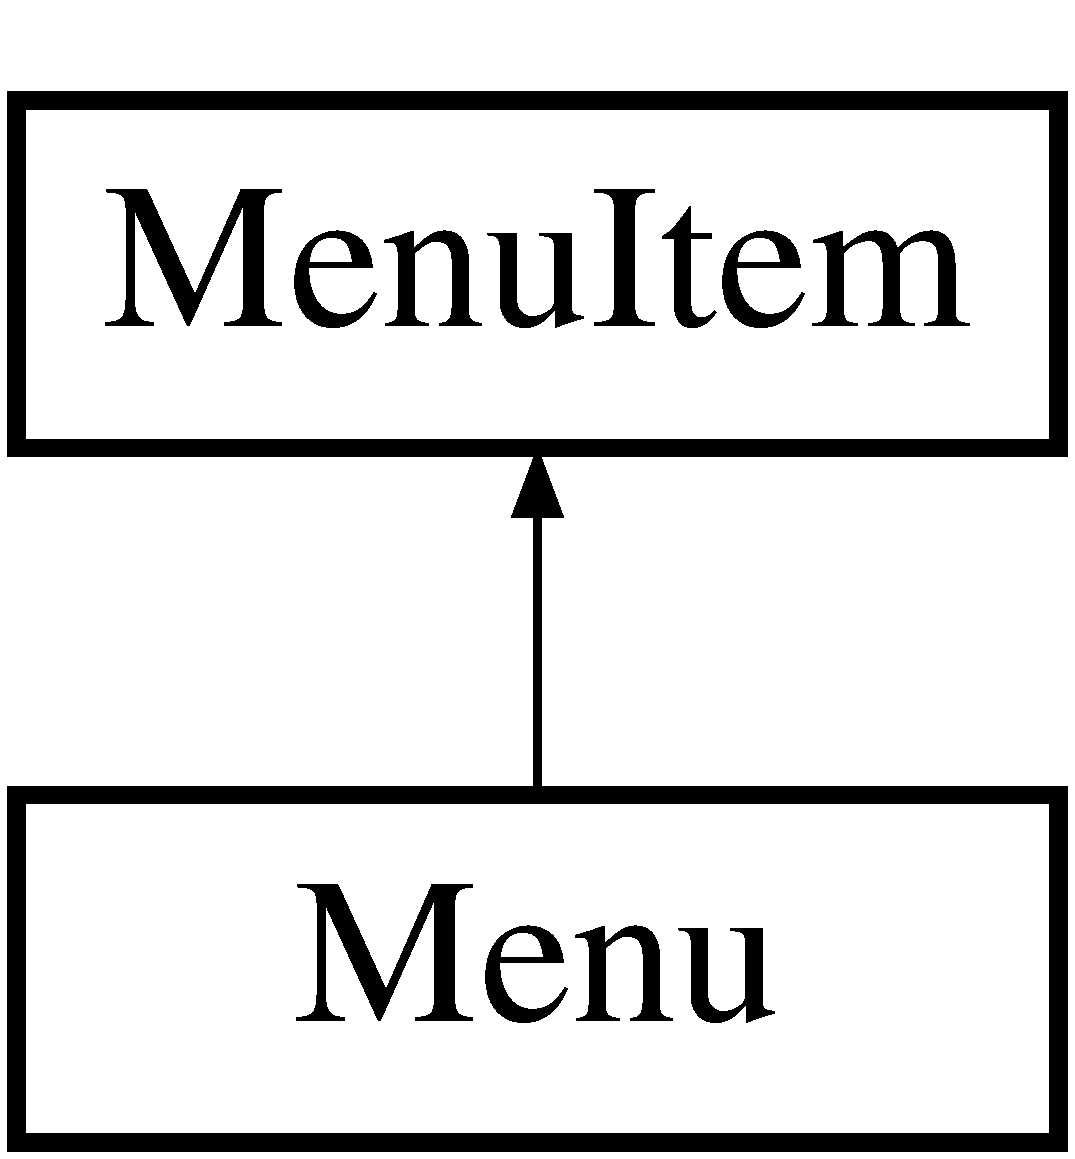
\includegraphics[height=2.000000cm]{class_menu}
\end{center}
\end{figure}
\subsection*{Public Member Functions}
\begin{DoxyCompactItemize}
\item 
\hyperlink{class_menu_aba4c387b52924a1c3cf43508e67a6412}{Menu} (char $\ast$name)
\item 
\hyperlink{class_menu_a831387f51358cfb88cd018e1777bc980}{$\sim$\+Menu} ()
\item 
void \hyperlink{class_menu_aa64e794ec331677883f6be3ec0e0eb5f}{Add\+Item} (\hyperlink{class_menu_item}{Menu\+Item} $\ast$item)
\item 
void \hyperlink{class_menu_a0be077217ae2c0735bd148e8359be21b}{Execute} (void)
\end{DoxyCompactItemize}
\subsection*{Additional Inherited Members}


\subsection{Constructor \& Destructor Documentation}
\mbox{\Hypertarget{class_menu_aba4c387b52924a1c3cf43508e67a6412}\label{class_menu_aba4c387b52924a1c3cf43508e67a6412}} 
\index{Menu@{Menu}!Menu@{Menu}}
\index{Menu@{Menu}!Menu@{Menu}}
\subsubsection{\texorpdfstring{Menu()}{Menu()}}
{\footnotesize\ttfamily Menu\+::\+Menu (\begin{DoxyParamCaption}\item[{char $\ast$}]{name }\end{DoxyParamCaption})}

\mbox{\Hypertarget{class_menu_a831387f51358cfb88cd018e1777bc980}\label{class_menu_a831387f51358cfb88cd018e1777bc980}} 
\index{Menu@{Menu}!````~Menu@{$\sim$\+Menu}}
\index{````~Menu@{$\sim$\+Menu}!Menu@{Menu}}
\subsubsection{\texorpdfstring{$\sim$\+Menu()}{~Menu()}}
{\footnotesize\ttfamily Menu\+::$\sim$\+Menu (\begin{DoxyParamCaption}{ }\end{DoxyParamCaption})}



\subsection{Member Function Documentation}
\mbox{\Hypertarget{class_menu_aa64e794ec331677883f6be3ec0e0eb5f}\label{class_menu_aa64e794ec331677883f6be3ec0e0eb5f}} 
\index{Menu@{Menu}!Add\+Item@{Add\+Item}}
\index{Add\+Item@{Add\+Item}!Menu@{Menu}}
\subsubsection{\texorpdfstring{Add\+Item()}{AddItem()}}
{\footnotesize\ttfamily void Menu\+::\+Add\+Item (\begin{DoxyParamCaption}\item[{\hyperlink{class_menu_item}{Menu\+Item} $\ast$}]{item }\end{DoxyParamCaption})}

\mbox{\Hypertarget{class_menu_a0be077217ae2c0735bd148e8359be21b}\label{class_menu_a0be077217ae2c0735bd148e8359be21b}} 
\index{Menu@{Menu}!Execute@{Execute}}
\index{Execute@{Execute}!Menu@{Menu}}
\subsubsection{\texorpdfstring{Execute()}{Execute()}}
{\footnotesize\ttfamily void Menu\+::\+Execute (\begin{DoxyParamCaption}\item[{void}]{ }\end{DoxyParamCaption})\hspace{0.3cm}{\ttfamily [virtual]}}



Implements \hyperlink{class_menu_item_a08f0695dbfdad36bc9aab7597df02a00}{Menu\+Item}.



The documentation for this class was generated from the following files\+:\begin{DoxyCompactItemize}
\item 
\hyperlink{_menu_8h}{Menu.\+h}\item 
\hyperlink{_menu_8cpp}{Menu.\+cpp}\end{DoxyCompactItemize}

\hypertarget{class_menu_item}{}\section{Menu\+Item Class Reference}
\label{class_menu_item}\index{Menu\+Item@{Menu\+Item}}


{\ttfamily \#include $<$Menu.\+h$>$}

Inheritance diagram for Menu\+Item\+:\begin{figure}[H]
\begin{center}
\leavevmode
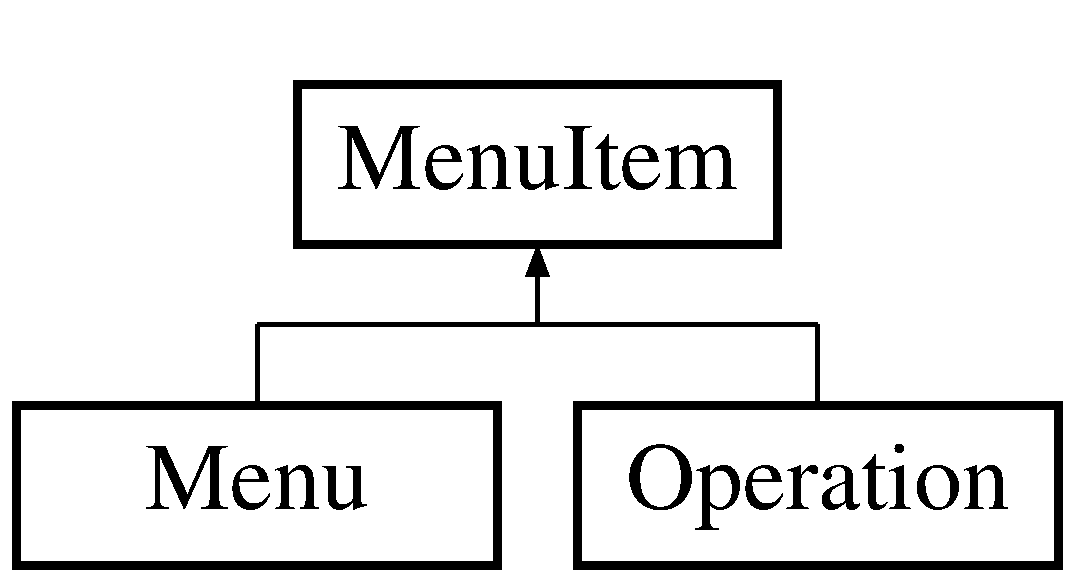
\includegraphics[height=2.000000cm]{class_menu_item}
\end{center}
\end{figure}
\subsection*{Public Member Functions}
\begin{DoxyCompactItemize}
\item 
char $\ast$ \hyperlink{class_menu_item_af23de886a192dede54b3254db5aa1830}{Get\+Name} (void)
\item 
virtual void \hyperlink{class_menu_item_a08f0695dbfdad36bc9aab7597df02a00}{Execute} (void)=0
\end{DoxyCompactItemize}
\subsection*{Protected Member Functions}
\begin{DoxyCompactItemize}
\item 
\hyperlink{class_menu_item_aa966696433faf0de75908d9789025f1f}{Menu\+Item} (char $\ast$name)
\item 
virtual \hyperlink{class_menu_item_a75a72b552ba092d7f0d24081648f5912}{$\sim$\+Menu\+Item} (void)
\item 
void \hyperlink{class_menu_item_aebc0f7620d970a978a24628adbfbe955}{Incomplete\+Title\+Display} (void)
\item 
void \hyperlink{class_menu_item_adbd2e567da57274ed67ed261a93fde56}{Display\+Title} (void)
\end{DoxyCompactItemize}
\subsection*{Friends}
\begin{DoxyCompactItemize}
\item 
class \hyperlink{class_menu_item_a834cec0fab7efabab3cd53540e4d466d}{Menu}
\end{DoxyCompactItemize}


\subsection{Constructor \& Destructor Documentation}
\mbox{\Hypertarget{class_menu_item_aa966696433faf0de75908d9789025f1f}\label{class_menu_item_aa966696433faf0de75908d9789025f1f}} 
\index{Menu\+Item@{Menu\+Item}!Menu\+Item@{Menu\+Item}}
\index{Menu\+Item@{Menu\+Item}!Menu\+Item@{Menu\+Item}}
\subsubsection{\texorpdfstring{Menu\+Item()}{MenuItem()}}
{\footnotesize\ttfamily Menu\+Item\+::\+Menu\+Item (\begin{DoxyParamCaption}\item[{char $\ast$}]{name }\end{DoxyParamCaption})\hspace{0.3cm}{\ttfamily [protected]}}

\mbox{\Hypertarget{class_menu_item_a75a72b552ba092d7f0d24081648f5912}\label{class_menu_item_a75a72b552ba092d7f0d24081648f5912}} 
\index{Menu\+Item@{Menu\+Item}!````~Menu\+Item@{$\sim$\+Menu\+Item}}
\index{````~Menu\+Item@{$\sim$\+Menu\+Item}!Menu\+Item@{Menu\+Item}}
\subsubsection{\texorpdfstring{$\sim$\+Menu\+Item()}{~MenuItem()}}
{\footnotesize\ttfamily Menu\+Item\+::$\sim$\+Menu\+Item (\begin{DoxyParamCaption}\item[{void}]{ }\end{DoxyParamCaption})\hspace{0.3cm}{\ttfamily [protected]}, {\ttfamily [virtual]}}



\subsection{Member Function Documentation}
\mbox{\Hypertarget{class_menu_item_adbd2e567da57274ed67ed261a93fde56}\label{class_menu_item_adbd2e567da57274ed67ed261a93fde56}} 
\index{Menu\+Item@{Menu\+Item}!Display\+Title@{Display\+Title}}
\index{Display\+Title@{Display\+Title}!Menu\+Item@{Menu\+Item}}
\subsubsection{\texorpdfstring{Display\+Title()}{DisplayTitle()}}
{\footnotesize\ttfamily void Menu\+Item\+::\+Display\+Title (\begin{DoxyParamCaption}\item[{void}]{ }\end{DoxyParamCaption})\hspace{0.3cm}{\ttfamily [protected]}}

\mbox{\Hypertarget{class_menu_item_a08f0695dbfdad36bc9aab7597df02a00}\label{class_menu_item_a08f0695dbfdad36bc9aab7597df02a00}} 
\index{Menu\+Item@{Menu\+Item}!Execute@{Execute}}
\index{Execute@{Execute}!Menu\+Item@{Menu\+Item}}
\subsubsection{\texorpdfstring{Execute()}{Execute()}}
{\footnotesize\ttfamily virtual void Menu\+Item\+::\+Execute (\begin{DoxyParamCaption}\item[{void}]{ }\end{DoxyParamCaption})\hspace{0.3cm}{\ttfamily [pure virtual]}}



Implemented in \hyperlink{class_menu_a0be077217ae2c0735bd148e8359be21b}{Menu}, and \hyperlink{class_operation_a669c894cc03d476fd8acecbf880dd606}{Operation}.

\mbox{\Hypertarget{class_menu_item_af23de886a192dede54b3254db5aa1830}\label{class_menu_item_af23de886a192dede54b3254db5aa1830}} 
\index{Menu\+Item@{Menu\+Item}!Get\+Name@{Get\+Name}}
\index{Get\+Name@{Get\+Name}!Menu\+Item@{Menu\+Item}}
\subsubsection{\texorpdfstring{Get\+Name()}{GetName()}}
{\footnotesize\ttfamily char $\ast$ Menu\+Item\+::\+Get\+Name (\begin{DoxyParamCaption}\item[{void}]{ }\end{DoxyParamCaption})}

\mbox{\Hypertarget{class_menu_item_aebc0f7620d970a978a24628adbfbe955}\label{class_menu_item_aebc0f7620d970a978a24628adbfbe955}} 
\index{Menu\+Item@{Menu\+Item}!Incomplete\+Title\+Display@{Incomplete\+Title\+Display}}
\index{Incomplete\+Title\+Display@{Incomplete\+Title\+Display}!Menu\+Item@{Menu\+Item}}
\subsubsection{\texorpdfstring{Incomplete\+Title\+Display()}{IncompleteTitleDisplay()}}
{\footnotesize\ttfamily void Menu\+Item\+::\+Incomplete\+Title\+Display (\begin{DoxyParamCaption}\item[{void}]{ }\end{DoxyParamCaption})\hspace{0.3cm}{\ttfamily [protected]}}



\subsection{Friends And Related Function Documentation}
\mbox{\Hypertarget{class_menu_item_a834cec0fab7efabab3cd53540e4d466d}\label{class_menu_item_a834cec0fab7efabab3cd53540e4d466d}} 
\index{Menu\+Item@{Menu\+Item}!Menu@{Menu}}
\index{Menu@{Menu}!Menu\+Item@{Menu\+Item}}
\subsubsection{\texorpdfstring{Menu}{Menu}}
{\footnotesize\ttfamily friend class \hyperlink{class_menu}{Menu}\hspace{0.3cm}{\ttfamily [friend]}}



The documentation for this class was generated from the following files\+:\begin{DoxyCompactItemize}
\item 
\hyperlink{_menu_8h}{Menu.\+h}\item 
\hyperlink{_menu_8cpp}{Menu.\+cpp}\end{DoxyCompactItemize}

\hypertarget{class_operation}{}\section{Operation Class Reference}
\label{class_operation}\index{Operation@{Operation}}


{\ttfamily \#include $<$Menu.\+h$>$}

Inheritance diagram for Operation\+:\begin{figure}[H]
\begin{center}
\leavevmode
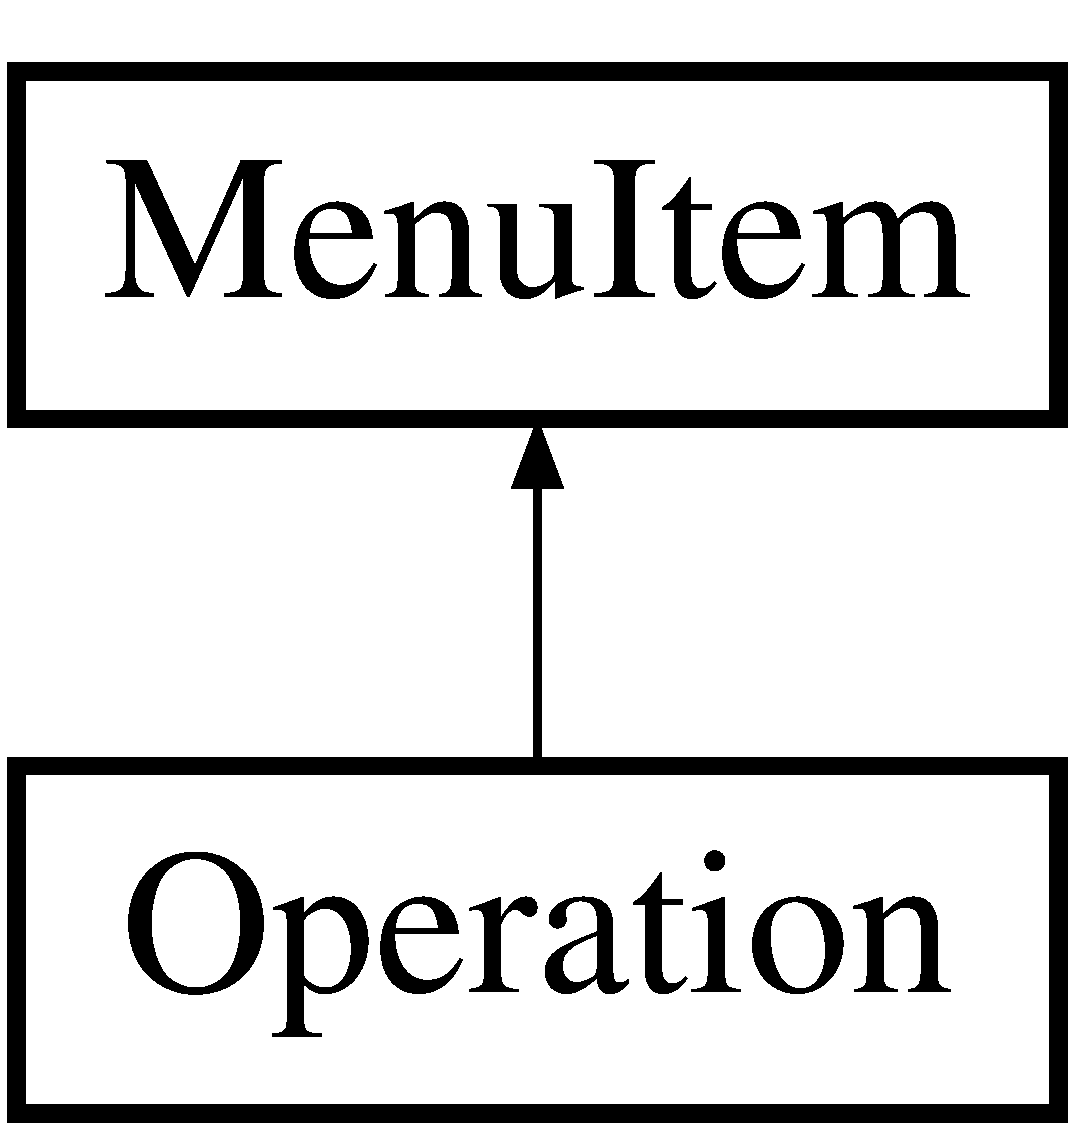
\includegraphics[height=2.000000cm]{class_operation}
\end{center}
\end{figure}
\subsection*{Public Member Functions}
\begin{DoxyCompactItemize}
\item 
void \hyperlink{class_operation_a669c894cc03d476fd8acecbf880dd606}{Execute} (void)
\end{DoxyCompactItemize}
\subsection*{Protected Member Functions}
\begin{DoxyCompactItemize}
\item 
\hyperlink{class_operation_a384d3cf47af8e48cf5199b93106d9d5f}{Operation} (char $\ast$name)
\item 
virtual void \hyperlink{class_operation_a40ffe4a0030abaf7db98f94515ccb17e}{Execute\+Operation} (void)=0
\end{DoxyCompactItemize}


\subsection{Constructor \& Destructor Documentation}
\mbox{\Hypertarget{class_operation_a384d3cf47af8e48cf5199b93106d9d5f}\label{class_operation_a384d3cf47af8e48cf5199b93106d9d5f}} 
\index{Operation@{Operation}!Operation@{Operation}}
\index{Operation@{Operation}!Operation@{Operation}}
\subsubsection{\texorpdfstring{Operation()}{Operation()}}
{\footnotesize\ttfamily Operation\+::\+Operation (\begin{DoxyParamCaption}\item[{char $\ast$}]{name }\end{DoxyParamCaption})\hspace{0.3cm}{\ttfamily [protected]}}



\subsection{Member Function Documentation}
\mbox{\Hypertarget{class_operation_a669c894cc03d476fd8acecbf880dd606}\label{class_operation_a669c894cc03d476fd8acecbf880dd606}} 
\index{Operation@{Operation}!Execute@{Execute}}
\index{Execute@{Execute}!Operation@{Operation}}
\subsubsection{\texorpdfstring{Execute()}{Execute()}}
{\footnotesize\ttfamily void Operation\+::\+Execute (\begin{DoxyParamCaption}\item[{void}]{ }\end{DoxyParamCaption})\hspace{0.3cm}{\ttfamily [virtual]}}



Implements \hyperlink{class_menu_item_a08f0695dbfdad36bc9aab7597df02a00}{Menu\+Item}.

\mbox{\Hypertarget{class_operation_a40ffe4a0030abaf7db98f94515ccb17e}\label{class_operation_a40ffe4a0030abaf7db98f94515ccb17e}} 
\index{Operation@{Operation}!Execute\+Operation@{Execute\+Operation}}
\index{Execute\+Operation@{Execute\+Operation}!Operation@{Operation}}
\subsubsection{\texorpdfstring{Execute\+Operation()}{ExecuteOperation()}}
{\footnotesize\ttfamily virtual void Operation\+::\+Execute\+Operation (\begin{DoxyParamCaption}\item[{void}]{ }\end{DoxyParamCaption})\hspace{0.3cm}{\ttfamily [protected]}, {\ttfamily [pure virtual]}}



The documentation for this class was generated from the following files\+:\begin{DoxyCompactItemize}
\item 
\hyperlink{_menu_8h}{Menu.\+h}\item 
\hyperlink{_menu_8cpp}{Menu.\+cpp}\end{DoxyCompactItemize}

\hypertarget{class_point}{}\section{Point Class Reference}
\label{class_point}\index{Point@{Point}}


{\ttfamily \#include $<$Figure.\+h$>$}

\subsection*{Public Types}
\begin{DoxyCompactItemize}
\item 
typedef double \hyperlink{class_point_a00b37528c0db634a12ecee9b29d79579}{point\+Type}
\end{DoxyCompactItemize}
\subsection*{Public Member Functions}
\begin{DoxyCompactItemize}
\item 
\hyperlink{class_point_ad92f2337b839a94ce97dcdb439b4325a}{Point} ()
\item 
\hyperlink{class_point_a4246ef6d69a6d29d1b9d1e225a9db964}{Point} (\hyperlink{class_point_a00b37528c0db634a12ecee9b29d79579}{point\+Type} p\+\_\+x, \hyperlink{class_point_a00b37528c0db634a12ecee9b29d79579}{point\+Type} p\+\_\+y)
\item 
double \hyperlink{class_point_a2707cf08d246f96e7ae16e6c1d6ce4f7}{distance\+To} (const \hyperlink{class_point}{Point} \&p)
\begin{DoxyCompactList}\small\item\em Euclidean distence between 2 points. \end{DoxyCompactList}\item 
\hyperlink{classtinyxml2_1_1_x_m_l_node}{tinyxml2\+::\+X\+M\+L\+Node} $\ast$ \hyperlink{class_point_a1d435eb5b4bc2bdaa92c596eb7728edc}{serialize} (\hyperlink{classtinyxml2_1_1_x_m_l_document}{tinyxml2\+::\+X\+M\+L\+Document} \&xml\+Doc)
\end{DoxyCompactItemize}
\subsection*{Public Attributes}
\begin{DoxyCompactItemize}
\item 
\hyperlink{class_point_a00b37528c0db634a12ecee9b29d79579}{point\+Type} \hyperlink{class_point_ae818271b839c768a11dfff7f3bf27b08}{y}
\item 
\hyperlink{class_point_a00b37528c0db634a12ecee9b29d79579}{point\+Type} \hyperlink{class_point_a76ee561a1b35e86084466b81b9835311}{x}
\end{DoxyCompactItemize}


\subsection{Member Typedef Documentation}
\mbox{\Hypertarget{class_point_a00b37528c0db634a12ecee9b29d79579}\label{class_point_a00b37528c0db634a12ecee9b29d79579}} 
\index{Point@{Point}!point\+Type@{point\+Type}}
\index{point\+Type@{point\+Type}!Point@{Point}}
\subsubsection{\texorpdfstring{point\+Type}{pointType}}
{\footnotesize\ttfamily typedef double \hyperlink{class_point_a00b37528c0db634a12ecee9b29d79579}{Point\+::point\+Type}}



\subsection{Constructor \& Destructor Documentation}
\mbox{\Hypertarget{class_point_ad92f2337b839a94ce97dcdb439b4325a}\label{class_point_ad92f2337b839a94ce97dcdb439b4325a}} 
\index{Point@{Point}!Point@{Point}}
\index{Point@{Point}!Point@{Point}}
\subsubsection{\texorpdfstring{Point()}{Point()}\hspace{0.1cm}{\footnotesize\ttfamily [1/2]}}
{\footnotesize\ttfamily Point\+::\+Point (\begin{DoxyParamCaption}{ }\end{DoxyParamCaption})}

\mbox{\Hypertarget{class_point_a4246ef6d69a6d29d1b9d1e225a9db964}\label{class_point_a4246ef6d69a6d29d1b9d1e225a9db964}} 
\index{Point@{Point}!Point@{Point}}
\index{Point@{Point}!Point@{Point}}
\subsubsection{\texorpdfstring{Point()}{Point()}\hspace{0.1cm}{\footnotesize\ttfamily [2/2]}}
{\footnotesize\ttfamily Point\+::\+Point (\begin{DoxyParamCaption}\item[{\hyperlink{class_point_a00b37528c0db634a12ecee9b29d79579}{point\+Type}}]{p\+\_\+x,  }\item[{\hyperlink{class_point_a00b37528c0db634a12ecee9b29d79579}{point\+Type}}]{p\+\_\+y }\end{DoxyParamCaption})}



\subsection{Member Function Documentation}
\mbox{\Hypertarget{class_point_a2707cf08d246f96e7ae16e6c1d6ce4f7}\label{class_point_a2707cf08d246f96e7ae16e6c1d6ce4f7}} 
\index{Point@{Point}!distance\+To@{distance\+To}}
\index{distance\+To@{distance\+To}!Point@{Point}}
\subsubsection{\texorpdfstring{distance\+To()}{distanceTo()}}
{\footnotesize\ttfamily double Point\+::distance\+To (\begin{DoxyParamCaption}\item[{const \hyperlink{class_point}{Point} \&}]{p }\end{DoxyParamCaption})}



Euclidean distence between 2 points. 

Evaluates sqrt((x\+\_\+b -\/ x\+\_\+a)$^\wedge$2 + (y\+\_\+b -\/ y\+\_\+a)$^\wedge$2) \mbox{\Hypertarget{class_point_a1d435eb5b4bc2bdaa92c596eb7728edc}\label{class_point_a1d435eb5b4bc2bdaa92c596eb7728edc}} 
\index{Point@{Point}!serialize@{serialize}}
\index{serialize@{serialize}!Point@{Point}}
\subsubsection{\texorpdfstring{serialize()}{serialize()}}
{\footnotesize\ttfamily \hyperlink{classtinyxml2_1_1_x_m_l_node}{tinyxml2\+::\+X\+M\+L\+Node} $\ast$ Point\+::serialize (\begin{DoxyParamCaption}\item[{\hyperlink{classtinyxml2_1_1_x_m_l_document}{tinyxml2\+::\+X\+M\+L\+Document} \&}]{xml\+Doc }\end{DoxyParamCaption})}



\subsection{Member Data Documentation}
\mbox{\Hypertarget{class_point_a76ee561a1b35e86084466b81b9835311}\label{class_point_a76ee561a1b35e86084466b81b9835311}} 
\index{Point@{Point}!x@{x}}
\index{x@{x}!Point@{Point}}
\subsubsection{\texorpdfstring{x}{x}}
{\footnotesize\ttfamily \hyperlink{class_point_a00b37528c0db634a12ecee9b29d79579}{point\+Type} Point\+::x}

\mbox{\Hypertarget{class_point_ae818271b839c768a11dfff7f3bf27b08}\label{class_point_ae818271b839c768a11dfff7f3bf27b08}} 
\index{Point@{Point}!y@{y}}
\index{y@{y}!Point@{Point}}
\subsubsection{\texorpdfstring{y}{y}}
{\footnotesize\ttfamily \hyperlink{class_point_a00b37528c0db634a12ecee9b29d79579}{point\+Type} Point\+::y}



The documentation for this class was generated from the following files\+:\begin{DoxyCompactItemize}
\item 
\hyperlink{_figure_8h}{Figure.\+h}\item 
\hyperlink{_figure_8cpp}{Figure.\+cpp}\end{DoxyCompactItemize}

\hypertarget{class_point_set}{}\section{Point\+Set Class Reference}
\label{class_point_set}\index{Point\+Set@{Point\+Set}}


{\ttfamily \#include $<$Point\+Set.\+h$>$}

Inheritance diagram for Point\+Set\+:\begin{figure}[H]
\begin{center}
\leavevmode
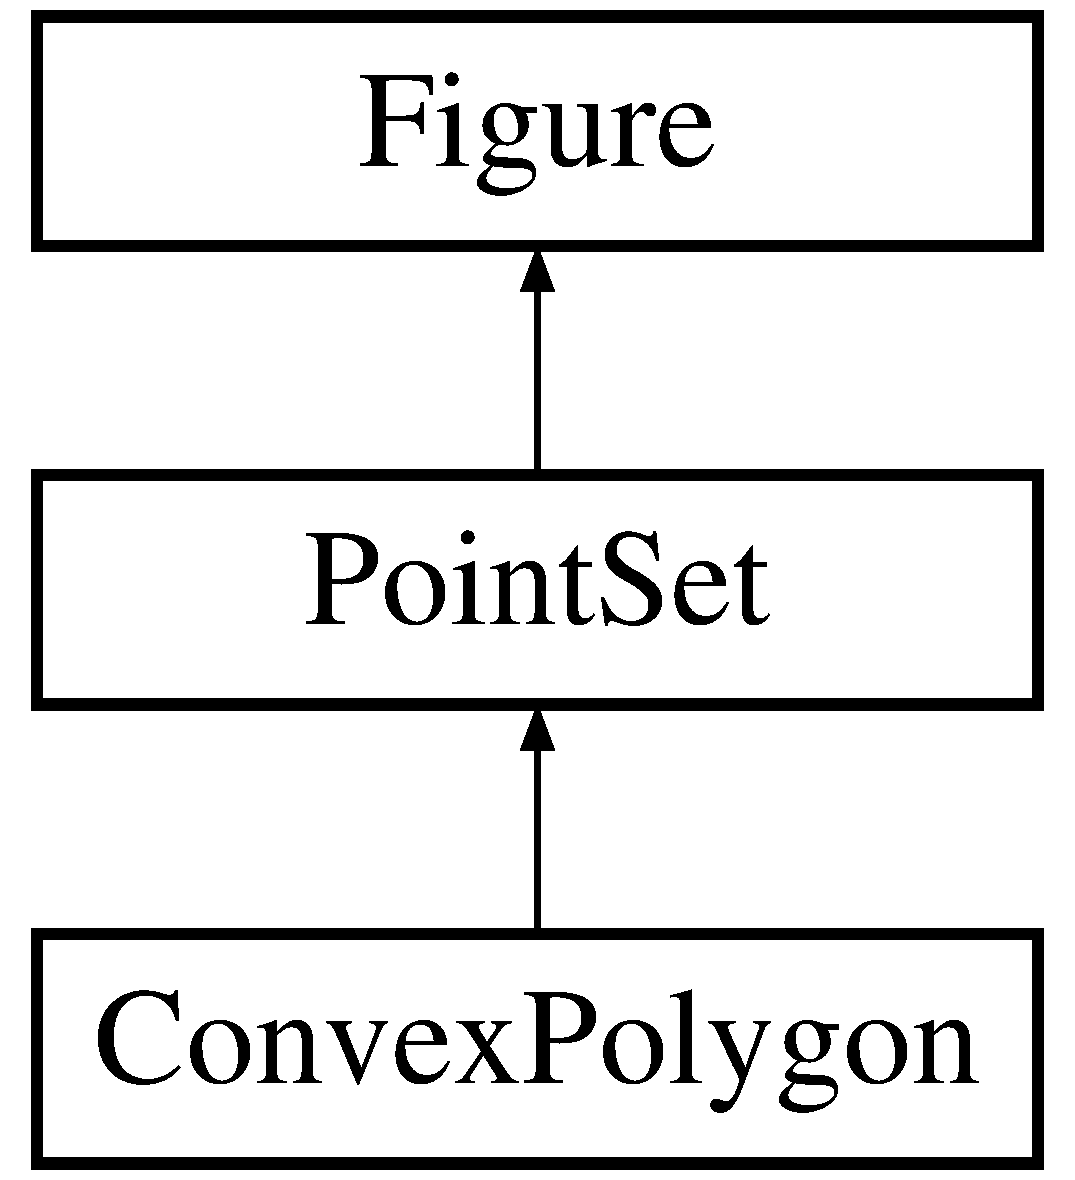
\includegraphics[height=3.000000cm]{class_point_set}
\end{center}
\end{figure}
\subsection*{Public Member Functions}
\begin{DoxyCompactItemize}
\item 
\hyperlink{class_point}{Point} \hyperlink{class_point_set_a61e0b486a1834af1158fecabaec4b4cb}{get\+Median\+Point} ()
\item 
unsigned \hyperlink{class_point_set_aa67d735f70d81ba36015d059573799c6}{get\+Point\+Nr} ()
\item 
\hyperlink{class_point_set_a0795eb5d1a45f7a5f3bc643f3866eb9f}{Point\+Set} ()
\item 
\hyperlink{class_point_set_ab50e8620e72c110c28bcdb9de78fcba2}{Point\+Set} (const \hyperlink{class_list}{List}$<$ \hyperlink{class_point}{Point} $>$ \&lst, const unsigned lst\+\_\+count)
\item 
virtual \hyperlink{class_point_set_a2ac2dc1fc77866357c8e1f1818019f61}{$\sim$\+Point\+Set} ()
\item 
virtual \hyperlink{classtinyxml2_1_1_x_m_l_node}{tinyxml2\+::\+X\+M\+L\+Node} $\ast$ \hyperlink{class_point_set_a282360046d7566f50d1ceec49aca0d89}{serialize} (\hyperlink{classtinyxml2_1_1_x_m_l_document}{tinyxml2\+::\+X\+M\+L\+Document} \&xml\+Doc)
\item 
double \hyperlink{class_point_set_aca8092b860a40743fb1c1189e8439764}{area} ()
\item 
double \hyperlink{class_point_set_a82b83d662bd5570e6e049e120e1c6bac}{perimeter} ()
\end{DoxyCompactItemize}
\subsection*{Protected Member Functions}
\begin{DoxyCompactItemize}
\item 
\hyperlink{class_list}{List}$<$ \hyperlink{class_point}{Point} $>$ \hyperlink{class_point_set_adef0a6be759d34e965aecb153a3e4b24}{get\+Points\+List} ()
\end{DoxyCompactItemize}
\subsection*{Protected Attributes}
\begin{DoxyCompactItemize}
\item 
\hyperlink{class_list}{List}$<$ \hyperlink{class_point}{Point} $>$ \hyperlink{class_point_set_a535724e3e1ffabf8d26009e555c32b21}{m\+\_\+points}
\item 
unsigned \hyperlink{class_point_set_ae2ba098c7108eb3ae954ca7d89a710f3}{m\+\_\+nr}
\end{DoxyCompactItemize}


\subsection{Constructor \& Destructor Documentation}
\mbox{\Hypertarget{class_point_set_a0795eb5d1a45f7a5f3bc643f3866eb9f}\label{class_point_set_a0795eb5d1a45f7a5f3bc643f3866eb9f}} 
\index{Point\+Set@{Point\+Set}!Point\+Set@{Point\+Set}}
\index{Point\+Set@{Point\+Set}!Point\+Set@{Point\+Set}}
\subsubsection{\texorpdfstring{Point\+Set()}{PointSet()}\hspace{0.1cm}{\footnotesize\ttfamily [1/2]}}
{\footnotesize\ttfamily Point\+Set\+::\+Point\+Set (\begin{DoxyParamCaption}{ }\end{DoxyParamCaption})}

\mbox{\Hypertarget{class_point_set_ab50e8620e72c110c28bcdb9de78fcba2}\label{class_point_set_ab50e8620e72c110c28bcdb9de78fcba2}} 
\index{Point\+Set@{Point\+Set}!Point\+Set@{Point\+Set}}
\index{Point\+Set@{Point\+Set}!Point\+Set@{Point\+Set}}
\subsubsection{\texorpdfstring{Point\+Set()}{PointSet()}\hspace{0.1cm}{\footnotesize\ttfamily [2/2]}}
{\footnotesize\ttfamily Point\+Set\+::\+Point\+Set (\begin{DoxyParamCaption}\item[{const \hyperlink{class_list}{List}$<$ \hyperlink{class_point}{Point} $>$ \&}]{lst,  }\item[{const unsigned}]{lst\+\_\+count }\end{DoxyParamCaption})}

\mbox{\Hypertarget{class_point_set_a2ac2dc1fc77866357c8e1f1818019f61}\label{class_point_set_a2ac2dc1fc77866357c8e1f1818019f61}} 
\index{Point\+Set@{Point\+Set}!````~Point\+Set@{$\sim$\+Point\+Set}}
\index{````~Point\+Set@{$\sim$\+Point\+Set}!Point\+Set@{Point\+Set}}
\subsubsection{\texorpdfstring{$\sim$\+Point\+Set()}{~PointSet()}}
{\footnotesize\ttfamily Point\+Set\+::$\sim$\+Point\+Set (\begin{DoxyParamCaption}{ }\end{DoxyParamCaption})\hspace{0.3cm}{\ttfamily [virtual]}}



\subsection{Member Function Documentation}
\mbox{\Hypertarget{class_point_set_aca8092b860a40743fb1c1189e8439764}\label{class_point_set_aca8092b860a40743fb1c1189e8439764}} 
\index{Point\+Set@{Point\+Set}!area@{area}}
\index{area@{area}!Point\+Set@{Point\+Set}}
\subsubsection{\texorpdfstring{area()}{area()}}
{\footnotesize\ttfamily double Point\+Set\+::area (\begin{DoxyParamCaption}{ }\end{DoxyParamCaption})\hspace{0.3cm}{\ttfamily [virtual]}}



Implements \hyperlink{class_figure_a9860bda67fc9ce8127a812e167c4ce75}{Figure}.

\mbox{\Hypertarget{class_point_set_a61e0b486a1834af1158fecabaec4b4cb}\label{class_point_set_a61e0b486a1834af1158fecabaec4b4cb}} 
\index{Point\+Set@{Point\+Set}!get\+Median\+Point@{get\+Median\+Point}}
\index{get\+Median\+Point@{get\+Median\+Point}!Point\+Set@{Point\+Set}}
\subsubsection{\texorpdfstring{get\+Median\+Point()}{getMedianPoint()}}
{\footnotesize\ttfamily \hyperlink{class_point}{Point} Point\+Set\+::get\+Median\+Point (\begin{DoxyParamCaption}{ }\end{DoxyParamCaption})}

\mbox{\Hypertarget{class_point_set_aa67d735f70d81ba36015d059573799c6}\label{class_point_set_aa67d735f70d81ba36015d059573799c6}} 
\index{Point\+Set@{Point\+Set}!get\+Point\+Nr@{get\+Point\+Nr}}
\index{get\+Point\+Nr@{get\+Point\+Nr}!Point\+Set@{Point\+Set}}
\subsubsection{\texorpdfstring{get\+Point\+Nr()}{getPointNr()}}
{\footnotesize\ttfamily unsigned Point\+Set\+::get\+Point\+Nr (\begin{DoxyParamCaption}{ }\end{DoxyParamCaption})}

\mbox{\Hypertarget{class_point_set_adef0a6be759d34e965aecb153a3e4b24}\label{class_point_set_adef0a6be759d34e965aecb153a3e4b24}} 
\index{Point\+Set@{Point\+Set}!get\+Points\+List@{get\+Points\+List}}
\index{get\+Points\+List@{get\+Points\+List}!Point\+Set@{Point\+Set}}
\subsubsection{\texorpdfstring{get\+Points\+List()}{getPointsList()}}
{\footnotesize\ttfamily \hyperlink{class_list}{List}$<$ \hyperlink{class_point}{Point} $>$ Point\+Set\+::get\+Points\+List (\begin{DoxyParamCaption}{ }\end{DoxyParamCaption})\hspace{0.3cm}{\ttfamily [protected]}}

\mbox{\Hypertarget{class_point_set_a82b83d662bd5570e6e049e120e1c6bac}\label{class_point_set_a82b83d662bd5570e6e049e120e1c6bac}} 
\index{Point\+Set@{Point\+Set}!perimeter@{perimeter}}
\index{perimeter@{perimeter}!Point\+Set@{Point\+Set}}
\subsubsection{\texorpdfstring{perimeter()}{perimeter()}}
{\footnotesize\ttfamily double Point\+Set\+::perimeter (\begin{DoxyParamCaption}{ }\end{DoxyParamCaption})\hspace{0.3cm}{\ttfamily [virtual]}}



Implements \hyperlink{class_figure_acae6802e2a55b322f7566f313d474546}{Figure}.

\mbox{\Hypertarget{class_point_set_a282360046d7566f50d1ceec49aca0d89}\label{class_point_set_a282360046d7566f50d1ceec49aca0d89}} 
\index{Point\+Set@{Point\+Set}!serialize@{serialize}}
\index{serialize@{serialize}!Point\+Set@{Point\+Set}}
\subsubsection{\texorpdfstring{serialize()}{serialize()}}
{\footnotesize\ttfamily \hyperlink{classtinyxml2_1_1_x_m_l_node}{tinyxml2\+::\+X\+M\+L\+Node} $\ast$ Point\+Set\+::serialize (\begin{DoxyParamCaption}\item[{\hyperlink{classtinyxml2_1_1_x_m_l_document}{tinyxml2\+::\+X\+M\+L\+Document} \&}]{xml\+Doc }\end{DoxyParamCaption})\hspace{0.3cm}{\ttfamily [virtual]}}



Implements \hyperlink{class_figure_a11994f67ee209a46047e0897680f6313}{Figure}.



Reimplemented in \hyperlink{class_convex_polygon_ab7cfd51933dd7a3bf821056c292ca62c}{Convex\+Polygon}.



\subsection{Member Data Documentation}
\mbox{\Hypertarget{class_point_set_ae2ba098c7108eb3ae954ca7d89a710f3}\label{class_point_set_ae2ba098c7108eb3ae954ca7d89a710f3}} 
\index{Point\+Set@{Point\+Set}!m\+\_\+nr@{m\+\_\+nr}}
\index{m\+\_\+nr@{m\+\_\+nr}!Point\+Set@{Point\+Set}}
\subsubsection{\texorpdfstring{m\+\_\+nr}{m\_nr}}
{\footnotesize\ttfamily unsigned Point\+Set\+::m\+\_\+nr\hspace{0.3cm}{\ttfamily [protected]}}

\mbox{\Hypertarget{class_point_set_a535724e3e1ffabf8d26009e555c32b21}\label{class_point_set_a535724e3e1ffabf8d26009e555c32b21}} 
\index{Point\+Set@{Point\+Set}!m\+\_\+points@{m\+\_\+points}}
\index{m\+\_\+points@{m\+\_\+points}!Point\+Set@{Point\+Set}}
\subsubsection{\texorpdfstring{m\+\_\+points}{m\_points}}
{\footnotesize\ttfamily \hyperlink{class_list}{List}$<$\hyperlink{class_point}{Point}$>$ Point\+Set\+::m\+\_\+points\hspace{0.3cm}{\ttfamily [protected]}}



The documentation for this class was generated from the following files\+:\begin{DoxyCompactItemize}
\item 
\hyperlink{_point_set_8h}{Point\+Set.\+h}\item 
\hyperlink{_point_set_8cpp}{Point\+Set.\+cpp}\end{DoxyCompactItemize}

\hypertarget{classtinyxml2_1_1_str_pair}{}\section{tinyxml2\+:\+:Str\+Pair Class Reference}
\label{classtinyxml2_1_1_str_pair}\index{tinyxml2\+::\+Str\+Pair@{tinyxml2\+::\+Str\+Pair}}


{\ttfamily \#include $<$tinyxml2.\+h$>$}

\subsection*{Public Types}
\begin{DoxyCompactItemize}
\item 
enum \{ \newline
\hyperlink{classtinyxml2_1_1_str_pair_a0301ef962e15dd94574431f1c61266c5a4f1e01a55f8efe4ca72c32d454060237}{N\+E\+E\+D\+S\+\_\+\+E\+N\+T\+I\+T\+Y\+\_\+\+P\+R\+O\+C\+E\+S\+S\+I\+NG} = 0x01, 
\hyperlink{classtinyxml2_1_1_str_pair_a0301ef962e15dd94574431f1c61266c5a8f2045d56e70745d718672c0da91d0e0}{N\+E\+E\+D\+S\+\_\+\+N\+E\+W\+L\+I\+N\+E\+\_\+\+N\+O\+R\+M\+A\+L\+I\+Z\+A\+T\+I\+ON} = 0x02, 
\hyperlink{classtinyxml2_1_1_str_pair_a0301ef962e15dd94574431f1c61266c5a13996e9d4ed18fd2d6af59bbab291b63}{N\+E\+E\+D\+S\+\_\+\+W\+H\+I\+T\+E\+S\+P\+A\+C\+E\+\_\+\+C\+O\+L\+L\+A\+P\+S\+I\+NG} = 0x04, 
\hyperlink{classtinyxml2_1_1_str_pair_a0301ef962e15dd94574431f1c61266c5aae519eb5a639858591763aa5fc6cc953}{T\+E\+X\+T\+\_\+\+E\+L\+E\+M\+E\+NT} = N\+E\+E\+D\+S\+\_\+\+E\+N\+T\+I\+T\+Y\+\_\+\+P\+R\+O\+C\+E\+S\+S\+I\+NG $\vert$ N\+E\+E\+D\+S\+\_\+\+N\+E\+W\+L\+I\+N\+E\+\_\+\+N\+O\+R\+M\+A\+L\+I\+Z\+A\+T\+I\+ON, 
\newline
\hyperlink{classtinyxml2_1_1_str_pair_a0301ef962e15dd94574431f1c61266c5a96be48cf899bfeea0aa227f984f1fa63}{T\+E\+X\+T\+\_\+\+E\+L\+E\+M\+E\+N\+T\+\_\+\+L\+E\+A\+V\+E\+\_\+\+E\+N\+T\+I\+T\+I\+ES} = N\+E\+E\+D\+S\+\_\+\+N\+E\+W\+L\+I\+N\+E\+\_\+\+N\+O\+R\+M\+A\+L\+I\+Z\+A\+T\+I\+ON, 
\hyperlink{classtinyxml2_1_1_str_pair_a0301ef962e15dd94574431f1c61266c5aaab1cbefaa977e6f772b4e2575417aeb}{A\+T\+T\+R\+I\+B\+U\+T\+E\+\_\+\+N\+A\+ME} = 0, 
\hyperlink{classtinyxml2_1_1_str_pair_a0301ef962e15dd94574431f1c61266c5a6d72f9ce15f50e8bcd680edf66235dfd}{A\+T\+T\+R\+I\+B\+U\+T\+E\+\_\+\+V\+A\+L\+UE} = N\+E\+E\+D\+S\+\_\+\+E\+N\+T\+I\+T\+Y\+\_\+\+P\+R\+O\+C\+E\+S\+S\+I\+NG $\vert$ N\+E\+E\+D\+S\+\_\+\+N\+E\+W\+L\+I\+N\+E\+\_\+\+N\+O\+R\+M\+A\+L\+I\+Z\+A\+T\+I\+ON, 
\hyperlink{classtinyxml2_1_1_str_pair_a0301ef962e15dd94574431f1c61266c5a2decbd2513ac14f8befa987938326399}{A\+T\+T\+R\+I\+B\+U\+T\+E\+\_\+\+V\+A\+L\+U\+E\+\_\+\+L\+E\+A\+V\+E\+\_\+\+E\+N\+T\+I\+T\+I\+ES} = N\+E\+E\+D\+S\+\_\+\+N\+E\+W\+L\+I\+N\+E\+\_\+\+N\+O\+R\+M\+A\+L\+I\+Z\+A\+T\+I\+ON, 
\newline
\hyperlink{classtinyxml2_1_1_str_pair_a0301ef962e15dd94574431f1c61266c5a067a6ec90c8beea1cf5992930d93bffa}{C\+O\+M\+M\+E\+NT} = N\+E\+E\+D\+S\+\_\+\+N\+E\+W\+L\+I\+N\+E\+\_\+\+N\+O\+R\+M\+A\+L\+I\+Z\+A\+T\+I\+ON
 \}
\end{DoxyCompactItemize}
\subsection*{Public Member Functions}
\begin{DoxyCompactItemize}
\item 
\hyperlink{classtinyxml2_1_1_str_pair_a69153963f7052de9f767d3d8c1623a70}{Str\+Pair} ()
\item 
\hyperlink{classtinyxml2_1_1_str_pair_a60bed84d2503296e1c2a73fcef1431f9}{$\sim$\+Str\+Pair} ()
\item 
void \hyperlink{classtinyxml2_1_1_str_pair_a4f05549373394266a1eecba26813c166}{Set} (char $\ast$start, char $\ast$end, int flags)
\item 
const char $\ast$ \hyperlink{classtinyxml2_1_1_str_pair_ad87e3d11330f5e689ba1e7e54c023b57}{Get\+Str} ()
\item 
bool \hyperlink{classtinyxml2_1_1_str_pair_aca963a7eaa900bfddbea7312f040b39c}{Empty} () const
\item 
void \hyperlink{classtinyxml2_1_1_str_pair_a2baf6230e18333e02ab65d0897ee3941}{Set\+Interned\+Str} (const char $\ast$str)
\item 
void \hyperlink{classtinyxml2_1_1_str_pair_a1f82ec6b5bee35ee7466d8565e43b1de}{Set\+Str} (const char $\ast$str, int flags=0)
\item 
char $\ast$ \hyperlink{classtinyxml2_1_1_str_pair_a68e6999b7677fa711287ececb9ba317e}{Parse\+Text} (char $\ast$in, const char $\ast$end\+Tag, int str\+Flags, int $\ast$cur\+Line\+Num\+Ptr)
\item 
char $\ast$ \hyperlink{classtinyxml2_1_1_str_pair_aa6d8998efceba41d87ec2300c70a6085}{Parse\+Name} (char $\ast$in)
\item 
void \hyperlink{classtinyxml2_1_1_str_pair_a35f795b1557fe5fdcbd93d3cc5d6b939}{Transfer\+To} (\hyperlink{classtinyxml2_1_1_str_pair}{Str\+Pair} $\ast$other)
\item 
void \hyperlink{classtinyxml2_1_1_str_pair_a80c1b3bd99bf62ae85c94a29ce537125}{Reset} ()
\end{DoxyCompactItemize}


\subsection{Member Enumeration Documentation}
\mbox{\Hypertarget{classtinyxml2_1_1_str_pair_a0301ef962e15dd94574431f1c61266c5}\label{classtinyxml2_1_1_str_pair_a0301ef962e15dd94574431f1c61266c5}} 
\subsubsection{\texorpdfstring{anonymous enum}{anonymous enum}}
{\footnotesize\ttfamily anonymous enum}

\begin{DoxyEnumFields}{Enumerator}
\raisebox{\heightof{T}}[0pt][0pt]{\index{N\+E\+E\+D\+S\+\_\+\+E\+N\+T\+I\+T\+Y\+\_\+\+P\+R\+O\+C\+E\+S\+S\+I\+NG@{N\+E\+E\+D\+S\+\_\+\+E\+N\+T\+I\+T\+Y\+\_\+\+P\+R\+O\+C\+E\+S\+S\+I\+NG}!tinyxml2\+::\+Str\+Pair@{tinyxml2\+::\+Str\+Pair}}\index{tinyxml2\+::\+Str\+Pair@{tinyxml2\+::\+Str\+Pair}!N\+E\+E\+D\+S\+\_\+\+E\+N\+T\+I\+T\+Y\+\_\+\+P\+R\+O\+C\+E\+S\+S\+I\+NG@{N\+E\+E\+D\+S\+\_\+\+E\+N\+T\+I\+T\+Y\+\_\+\+P\+R\+O\+C\+E\+S\+S\+I\+NG}}}\mbox{\Hypertarget{classtinyxml2_1_1_str_pair_a0301ef962e15dd94574431f1c61266c5a4f1e01a55f8efe4ca72c32d454060237}\label{classtinyxml2_1_1_str_pair_a0301ef962e15dd94574431f1c61266c5a4f1e01a55f8efe4ca72c32d454060237}} 
N\+E\+E\+D\+S\+\_\+\+E\+N\+T\+I\+T\+Y\+\_\+\+P\+R\+O\+C\+E\+S\+S\+I\+NG&\\
\hline

\raisebox{\heightof{T}}[0pt][0pt]{\index{N\+E\+E\+D\+S\+\_\+\+N\+E\+W\+L\+I\+N\+E\+\_\+\+N\+O\+R\+M\+A\+L\+I\+Z\+A\+T\+I\+ON@{N\+E\+E\+D\+S\+\_\+\+N\+E\+W\+L\+I\+N\+E\+\_\+\+N\+O\+R\+M\+A\+L\+I\+Z\+A\+T\+I\+ON}!tinyxml2\+::\+Str\+Pair@{tinyxml2\+::\+Str\+Pair}}\index{tinyxml2\+::\+Str\+Pair@{tinyxml2\+::\+Str\+Pair}!N\+E\+E\+D\+S\+\_\+\+N\+E\+W\+L\+I\+N\+E\+\_\+\+N\+O\+R\+M\+A\+L\+I\+Z\+A\+T\+I\+ON@{N\+E\+E\+D\+S\+\_\+\+N\+E\+W\+L\+I\+N\+E\+\_\+\+N\+O\+R\+M\+A\+L\+I\+Z\+A\+T\+I\+ON}}}\mbox{\Hypertarget{classtinyxml2_1_1_str_pair_a0301ef962e15dd94574431f1c61266c5a8f2045d56e70745d718672c0da91d0e0}\label{classtinyxml2_1_1_str_pair_a0301ef962e15dd94574431f1c61266c5a8f2045d56e70745d718672c0da91d0e0}} 
N\+E\+E\+D\+S\+\_\+\+N\+E\+W\+L\+I\+N\+E\+\_\+\+N\+O\+R\+M\+A\+L\+I\+Z\+A\+T\+I\+ON&\\
\hline

\raisebox{\heightof{T}}[0pt][0pt]{\index{N\+E\+E\+D\+S\+\_\+\+W\+H\+I\+T\+E\+S\+P\+A\+C\+E\+\_\+\+C\+O\+L\+L\+A\+P\+S\+I\+NG@{N\+E\+E\+D\+S\+\_\+\+W\+H\+I\+T\+E\+S\+P\+A\+C\+E\+\_\+\+C\+O\+L\+L\+A\+P\+S\+I\+NG}!tinyxml2\+::\+Str\+Pair@{tinyxml2\+::\+Str\+Pair}}\index{tinyxml2\+::\+Str\+Pair@{tinyxml2\+::\+Str\+Pair}!N\+E\+E\+D\+S\+\_\+\+W\+H\+I\+T\+E\+S\+P\+A\+C\+E\+\_\+\+C\+O\+L\+L\+A\+P\+S\+I\+NG@{N\+E\+E\+D\+S\+\_\+\+W\+H\+I\+T\+E\+S\+P\+A\+C\+E\+\_\+\+C\+O\+L\+L\+A\+P\+S\+I\+NG}}}\mbox{\Hypertarget{classtinyxml2_1_1_str_pair_a0301ef962e15dd94574431f1c61266c5a13996e9d4ed18fd2d6af59bbab291b63}\label{classtinyxml2_1_1_str_pair_a0301ef962e15dd94574431f1c61266c5a13996e9d4ed18fd2d6af59bbab291b63}} 
N\+E\+E\+D\+S\+\_\+\+W\+H\+I\+T\+E\+S\+P\+A\+C\+E\+\_\+\+C\+O\+L\+L\+A\+P\+S\+I\+NG&\\
\hline

\raisebox{\heightof{T}}[0pt][0pt]{\index{T\+E\+X\+T\+\_\+\+E\+L\+E\+M\+E\+NT@{T\+E\+X\+T\+\_\+\+E\+L\+E\+M\+E\+NT}!tinyxml2\+::\+Str\+Pair@{tinyxml2\+::\+Str\+Pair}}\index{tinyxml2\+::\+Str\+Pair@{tinyxml2\+::\+Str\+Pair}!T\+E\+X\+T\+\_\+\+E\+L\+E\+M\+E\+NT@{T\+E\+X\+T\+\_\+\+E\+L\+E\+M\+E\+NT}}}\mbox{\Hypertarget{classtinyxml2_1_1_str_pair_a0301ef962e15dd94574431f1c61266c5aae519eb5a639858591763aa5fc6cc953}\label{classtinyxml2_1_1_str_pair_a0301ef962e15dd94574431f1c61266c5aae519eb5a639858591763aa5fc6cc953}} 
T\+E\+X\+T\+\_\+\+E\+L\+E\+M\+E\+NT&\\
\hline

\raisebox{\heightof{T}}[0pt][0pt]{\index{T\+E\+X\+T\+\_\+\+E\+L\+E\+M\+E\+N\+T\+\_\+\+L\+E\+A\+V\+E\+\_\+\+E\+N\+T\+I\+T\+I\+ES@{T\+E\+X\+T\+\_\+\+E\+L\+E\+M\+E\+N\+T\+\_\+\+L\+E\+A\+V\+E\+\_\+\+E\+N\+T\+I\+T\+I\+ES}!tinyxml2\+::\+Str\+Pair@{tinyxml2\+::\+Str\+Pair}}\index{tinyxml2\+::\+Str\+Pair@{tinyxml2\+::\+Str\+Pair}!T\+E\+X\+T\+\_\+\+E\+L\+E\+M\+E\+N\+T\+\_\+\+L\+E\+A\+V\+E\+\_\+\+E\+N\+T\+I\+T\+I\+ES@{T\+E\+X\+T\+\_\+\+E\+L\+E\+M\+E\+N\+T\+\_\+\+L\+E\+A\+V\+E\+\_\+\+E\+N\+T\+I\+T\+I\+ES}}}\mbox{\Hypertarget{classtinyxml2_1_1_str_pair_a0301ef962e15dd94574431f1c61266c5a96be48cf899bfeea0aa227f984f1fa63}\label{classtinyxml2_1_1_str_pair_a0301ef962e15dd94574431f1c61266c5a96be48cf899bfeea0aa227f984f1fa63}} 
T\+E\+X\+T\+\_\+\+E\+L\+E\+M\+E\+N\+T\+\_\+\+L\+E\+A\+V\+E\+\_\+\+E\+N\+T\+I\+T\+I\+ES&\\
\hline

\raisebox{\heightof{T}}[0pt][0pt]{\index{A\+T\+T\+R\+I\+B\+U\+T\+E\+\_\+\+N\+A\+ME@{A\+T\+T\+R\+I\+B\+U\+T\+E\+\_\+\+N\+A\+ME}!tinyxml2\+::\+Str\+Pair@{tinyxml2\+::\+Str\+Pair}}\index{tinyxml2\+::\+Str\+Pair@{tinyxml2\+::\+Str\+Pair}!A\+T\+T\+R\+I\+B\+U\+T\+E\+\_\+\+N\+A\+ME@{A\+T\+T\+R\+I\+B\+U\+T\+E\+\_\+\+N\+A\+ME}}}\mbox{\Hypertarget{classtinyxml2_1_1_str_pair_a0301ef962e15dd94574431f1c61266c5aaab1cbefaa977e6f772b4e2575417aeb}\label{classtinyxml2_1_1_str_pair_a0301ef962e15dd94574431f1c61266c5aaab1cbefaa977e6f772b4e2575417aeb}} 
A\+T\+T\+R\+I\+B\+U\+T\+E\+\_\+\+N\+A\+ME&\\
\hline

\raisebox{\heightof{T}}[0pt][0pt]{\index{A\+T\+T\+R\+I\+B\+U\+T\+E\+\_\+\+V\+A\+L\+UE@{A\+T\+T\+R\+I\+B\+U\+T\+E\+\_\+\+V\+A\+L\+UE}!tinyxml2\+::\+Str\+Pair@{tinyxml2\+::\+Str\+Pair}}\index{tinyxml2\+::\+Str\+Pair@{tinyxml2\+::\+Str\+Pair}!A\+T\+T\+R\+I\+B\+U\+T\+E\+\_\+\+V\+A\+L\+UE@{A\+T\+T\+R\+I\+B\+U\+T\+E\+\_\+\+V\+A\+L\+UE}}}\mbox{\Hypertarget{classtinyxml2_1_1_str_pair_a0301ef962e15dd94574431f1c61266c5a6d72f9ce15f50e8bcd680edf66235dfd}\label{classtinyxml2_1_1_str_pair_a0301ef962e15dd94574431f1c61266c5a6d72f9ce15f50e8bcd680edf66235dfd}} 
A\+T\+T\+R\+I\+B\+U\+T\+E\+\_\+\+V\+A\+L\+UE&\\
\hline

\raisebox{\heightof{T}}[0pt][0pt]{\index{A\+T\+T\+R\+I\+B\+U\+T\+E\+\_\+\+V\+A\+L\+U\+E\+\_\+\+L\+E\+A\+V\+E\+\_\+\+E\+N\+T\+I\+T\+I\+ES@{A\+T\+T\+R\+I\+B\+U\+T\+E\+\_\+\+V\+A\+L\+U\+E\+\_\+\+L\+E\+A\+V\+E\+\_\+\+E\+N\+T\+I\+T\+I\+ES}!tinyxml2\+::\+Str\+Pair@{tinyxml2\+::\+Str\+Pair}}\index{tinyxml2\+::\+Str\+Pair@{tinyxml2\+::\+Str\+Pair}!A\+T\+T\+R\+I\+B\+U\+T\+E\+\_\+\+V\+A\+L\+U\+E\+\_\+\+L\+E\+A\+V\+E\+\_\+\+E\+N\+T\+I\+T\+I\+ES@{A\+T\+T\+R\+I\+B\+U\+T\+E\+\_\+\+V\+A\+L\+U\+E\+\_\+\+L\+E\+A\+V\+E\+\_\+\+E\+N\+T\+I\+T\+I\+ES}}}\mbox{\Hypertarget{classtinyxml2_1_1_str_pair_a0301ef962e15dd94574431f1c61266c5a2decbd2513ac14f8befa987938326399}\label{classtinyxml2_1_1_str_pair_a0301ef962e15dd94574431f1c61266c5a2decbd2513ac14f8befa987938326399}} 
A\+T\+T\+R\+I\+B\+U\+T\+E\+\_\+\+V\+A\+L\+U\+E\+\_\+\+L\+E\+A\+V\+E\+\_\+\+E\+N\+T\+I\+T\+I\+ES&\\
\hline

\raisebox{\heightof{T}}[0pt][0pt]{\index{C\+O\+M\+M\+E\+NT@{C\+O\+M\+M\+E\+NT}!tinyxml2\+::\+Str\+Pair@{tinyxml2\+::\+Str\+Pair}}\index{tinyxml2\+::\+Str\+Pair@{tinyxml2\+::\+Str\+Pair}!C\+O\+M\+M\+E\+NT@{C\+O\+M\+M\+E\+NT}}}\mbox{\Hypertarget{classtinyxml2_1_1_str_pair_a0301ef962e15dd94574431f1c61266c5a067a6ec90c8beea1cf5992930d93bffa}\label{classtinyxml2_1_1_str_pair_a0301ef962e15dd94574431f1c61266c5a067a6ec90c8beea1cf5992930d93bffa}} 
C\+O\+M\+M\+E\+NT&\\
\hline

\end{DoxyEnumFields}


\subsection{Constructor \& Destructor Documentation}
\mbox{\Hypertarget{classtinyxml2_1_1_str_pair_a69153963f7052de9f767d3d8c1623a70}\label{classtinyxml2_1_1_str_pair_a69153963f7052de9f767d3d8c1623a70}} 
\index{tinyxml2\+::\+Str\+Pair@{tinyxml2\+::\+Str\+Pair}!Str\+Pair@{Str\+Pair}}
\index{Str\+Pair@{Str\+Pair}!tinyxml2\+::\+Str\+Pair@{tinyxml2\+::\+Str\+Pair}}
\subsubsection{\texorpdfstring{Str\+Pair()}{StrPair()}}
{\footnotesize\ttfamily tinyxml2\+::\+Str\+Pair\+::\+Str\+Pair (\begin{DoxyParamCaption}{ }\end{DoxyParamCaption})\hspace{0.3cm}{\ttfamily [inline]}}

\mbox{\Hypertarget{classtinyxml2_1_1_str_pair_a60bed84d2503296e1c2a73fcef1431f9}\label{classtinyxml2_1_1_str_pair_a60bed84d2503296e1c2a73fcef1431f9}} 
\index{tinyxml2\+::\+Str\+Pair@{tinyxml2\+::\+Str\+Pair}!````~Str\+Pair@{$\sim$\+Str\+Pair}}
\index{````~Str\+Pair@{$\sim$\+Str\+Pair}!tinyxml2\+::\+Str\+Pair@{tinyxml2\+::\+Str\+Pair}}
\subsubsection{\texorpdfstring{$\sim$\+Str\+Pair()}{~StrPair()}}
{\footnotesize\ttfamily tinyxml2\+::\+Str\+Pair\+::$\sim$\+Str\+Pair (\begin{DoxyParamCaption}{ }\end{DoxyParamCaption})}



\subsection{Member Function Documentation}
\mbox{\Hypertarget{classtinyxml2_1_1_str_pair_aca963a7eaa900bfddbea7312f040b39c}\label{classtinyxml2_1_1_str_pair_aca963a7eaa900bfddbea7312f040b39c}} 
\index{tinyxml2\+::\+Str\+Pair@{tinyxml2\+::\+Str\+Pair}!Empty@{Empty}}
\index{Empty@{Empty}!tinyxml2\+::\+Str\+Pair@{tinyxml2\+::\+Str\+Pair}}
\subsubsection{\texorpdfstring{Empty()}{Empty()}}
{\footnotesize\ttfamily bool tinyxml2\+::\+Str\+Pair\+::\+Empty (\begin{DoxyParamCaption}{ }\end{DoxyParamCaption}) const\hspace{0.3cm}{\ttfamily [inline]}}

\mbox{\Hypertarget{classtinyxml2_1_1_str_pair_ad87e3d11330f5e689ba1e7e54c023b57}\label{classtinyxml2_1_1_str_pair_ad87e3d11330f5e689ba1e7e54c023b57}} 
\index{tinyxml2\+::\+Str\+Pair@{tinyxml2\+::\+Str\+Pair}!Get\+Str@{Get\+Str}}
\index{Get\+Str@{Get\+Str}!tinyxml2\+::\+Str\+Pair@{tinyxml2\+::\+Str\+Pair}}
\subsubsection{\texorpdfstring{Get\+Str()}{GetStr()}}
{\footnotesize\ttfamily const char $\ast$ tinyxml2\+::\+Str\+Pair\+::\+Get\+Str (\begin{DoxyParamCaption}{ }\end{DoxyParamCaption})}

\mbox{\Hypertarget{classtinyxml2_1_1_str_pair_aa6d8998efceba41d87ec2300c70a6085}\label{classtinyxml2_1_1_str_pair_aa6d8998efceba41d87ec2300c70a6085}} 
\index{tinyxml2\+::\+Str\+Pair@{tinyxml2\+::\+Str\+Pair}!Parse\+Name@{Parse\+Name}}
\index{Parse\+Name@{Parse\+Name}!tinyxml2\+::\+Str\+Pair@{tinyxml2\+::\+Str\+Pair}}
\subsubsection{\texorpdfstring{Parse\+Name()}{ParseName()}}
{\footnotesize\ttfamily char $\ast$ tinyxml2\+::\+Str\+Pair\+::\+Parse\+Name (\begin{DoxyParamCaption}\item[{char $\ast$}]{in }\end{DoxyParamCaption})}

\mbox{\Hypertarget{classtinyxml2_1_1_str_pair_a68e6999b7677fa711287ececb9ba317e}\label{classtinyxml2_1_1_str_pair_a68e6999b7677fa711287ececb9ba317e}} 
\index{tinyxml2\+::\+Str\+Pair@{tinyxml2\+::\+Str\+Pair}!Parse\+Text@{Parse\+Text}}
\index{Parse\+Text@{Parse\+Text}!tinyxml2\+::\+Str\+Pair@{tinyxml2\+::\+Str\+Pair}}
\subsubsection{\texorpdfstring{Parse\+Text()}{ParseText()}}
{\footnotesize\ttfamily char $\ast$ tinyxml2\+::\+Str\+Pair\+::\+Parse\+Text (\begin{DoxyParamCaption}\item[{char $\ast$}]{in,  }\item[{const char $\ast$}]{end\+Tag,  }\item[{int}]{str\+Flags,  }\item[{int $\ast$}]{cur\+Line\+Num\+Ptr }\end{DoxyParamCaption})}

\mbox{\Hypertarget{classtinyxml2_1_1_str_pair_a80c1b3bd99bf62ae85c94a29ce537125}\label{classtinyxml2_1_1_str_pair_a80c1b3bd99bf62ae85c94a29ce537125}} 
\index{tinyxml2\+::\+Str\+Pair@{tinyxml2\+::\+Str\+Pair}!Reset@{Reset}}
\index{Reset@{Reset}!tinyxml2\+::\+Str\+Pair@{tinyxml2\+::\+Str\+Pair}}
\subsubsection{\texorpdfstring{Reset()}{Reset()}}
{\footnotesize\ttfamily void tinyxml2\+::\+Str\+Pair\+::\+Reset (\begin{DoxyParamCaption}{ }\end{DoxyParamCaption})}

\mbox{\Hypertarget{classtinyxml2_1_1_str_pair_a4f05549373394266a1eecba26813c166}\label{classtinyxml2_1_1_str_pair_a4f05549373394266a1eecba26813c166}} 
\index{tinyxml2\+::\+Str\+Pair@{tinyxml2\+::\+Str\+Pair}!Set@{Set}}
\index{Set@{Set}!tinyxml2\+::\+Str\+Pair@{tinyxml2\+::\+Str\+Pair}}
\subsubsection{\texorpdfstring{Set()}{Set()}}
{\footnotesize\ttfamily void tinyxml2\+::\+Str\+Pair\+::\+Set (\begin{DoxyParamCaption}\item[{char $\ast$}]{start,  }\item[{char $\ast$}]{end,  }\item[{int}]{flags }\end{DoxyParamCaption})\hspace{0.3cm}{\ttfamily [inline]}}

\mbox{\Hypertarget{classtinyxml2_1_1_str_pair_a2baf6230e18333e02ab65d0897ee3941}\label{classtinyxml2_1_1_str_pair_a2baf6230e18333e02ab65d0897ee3941}} 
\index{tinyxml2\+::\+Str\+Pair@{tinyxml2\+::\+Str\+Pair}!Set\+Interned\+Str@{Set\+Interned\+Str}}
\index{Set\+Interned\+Str@{Set\+Interned\+Str}!tinyxml2\+::\+Str\+Pair@{tinyxml2\+::\+Str\+Pair}}
\subsubsection{\texorpdfstring{Set\+Interned\+Str()}{SetInternedStr()}}
{\footnotesize\ttfamily void tinyxml2\+::\+Str\+Pair\+::\+Set\+Interned\+Str (\begin{DoxyParamCaption}\item[{const char $\ast$}]{str }\end{DoxyParamCaption})\hspace{0.3cm}{\ttfamily [inline]}}

\mbox{\Hypertarget{classtinyxml2_1_1_str_pair_a1f82ec6b5bee35ee7466d8565e43b1de}\label{classtinyxml2_1_1_str_pair_a1f82ec6b5bee35ee7466d8565e43b1de}} 
\index{tinyxml2\+::\+Str\+Pair@{tinyxml2\+::\+Str\+Pair}!Set\+Str@{Set\+Str}}
\index{Set\+Str@{Set\+Str}!tinyxml2\+::\+Str\+Pair@{tinyxml2\+::\+Str\+Pair}}
\subsubsection{\texorpdfstring{Set\+Str()}{SetStr()}}
{\footnotesize\ttfamily void tinyxml2\+::\+Str\+Pair\+::\+Set\+Str (\begin{DoxyParamCaption}\item[{const char $\ast$}]{str,  }\item[{int}]{flags = {\ttfamily 0} }\end{DoxyParamCaption})}

\mbox{\Hypertarget{classtinyxml2_1_1_str_pair_a35f795b1557fe5fdcbd93d3cc5d6b939}\label{classtinyxml2_1_1_str_pair_a35f795b1557fe5fdcbd93d3cc5d6b939}} 
\index{tinyxml2\+::\+Str\+Pair@{tinyxml2\+::\+Str\+Pair}!Transfer\+To@{Transfer\+To}}
\index{Transfer\+To@{Transfer\+To}!tinyxml2\+::\+Str\+Pair@{tinyxml2\+::\+Str\+Pair}}
\subsubsection{\texorpdfstring{Transfer\+To()}{TransferTo()}}
{\footnotesize\ttfamily void tinyxml2\+::\+Str\+Pair\+::\+Transfer\+To (\begin{DoxyParamCaption}\item[{\hyperlink{classtinyxml2_1_1_str_pair}{Str\+Pair} $\ast$}]{other }\end{DoxyParamCaption})}



The documentation for this class was generated from the following files\+:\begin{DoxyCompactItemize}
\item 
\hyperlink{tinyxml2_8h}{tinyxml2.\+h}\item 
\hyperlink{tinyxml2_8cpp}{tinyxml2.\+cpp}\end{DoxyCompactItemize}

\hypertarget{classtinyxml2_1_1_x_m_l_attribute}{}\section{tinyxml2\+:\+:X\+M\+L\+Attribute Class Reference}
\label{classtinyxml2_1_1_x_m_l_attribute}\index{tinyxml2\+::\+X\+M\+L\+Attribute@{tinyxml2\+::\+X\+M\+L\+Attribute}}


{\ttfamily \#include $<$tinyxml2.\+h$>$}

\subsection*{Public Member Functions}
\begin{DoxyCompactItemize}
\item 
const char $\ast$ \hyperlink{classtinyxml2_1_1_x_m_l_attribute_a5a5c135d24cce7abda6f17301c6274d8}{Name} () const
\begin{DoxyCompactList}\small\item\em The name of the attribute. \end{DoxyCompactList}\item 
const char $\ast$ \hyperlink{classtinyxml2_1_1_x_m_l_attribute_ab1c5cd993f836a771818ca408994b14e}{Value} () const
\begin{DoxyCompactList}\small\item\em The value of the attribute. \end{DoxyCompactList}\item 
int \hyperlink{classtinyxml2_1_1_x_m_l_attribute_a02d5ea924586e35f9c13857d1671b765}{Get\+Line\+Num} () const
\begin{DoxyCompactList}\small\item\em Gets the line number the attribute is in, if the document was parsed from a file. \end{DoxyCompactList}\item 
const \hyperlink{classtinyxml2_1_1_x_m_l_attribute}{X\+M\+L\+Attribute} $\ast$ \hyperlink{classtinyxml2_1_1_x_m_l_attribute_aee53571b21e7ce5421eb929523a8bbe6}{Next} () const
\begin{DoxyCompactList}\small\item\em The next attribute in the list. \end{DoxyCompactList}\item 
int \hyperlink{classtinyxml2_1_1_x_m_l_attribute_adfa2433f0fdafd5c3880936de9affa80}{Int\+Value} () const
\item 
int64\+\_\+t \hyperlink{classtinyxml2_1_1_x_m_l_attribute_a8762ed54f147c5744ada55c3d04d27f2}{Int64\+Value} () const
\item 
unsigned \hyperlink{classtinyxml2_1_1_x_m_l_attribute_a0be5343b08a957c42c02c5d32c35d338}{Unsigned\+Value} () const
\begin{DoxyCompactList}\small\item\em Query as an unsigned integer. See \hyperlink{classtinyxml2_1_1_x_m_l_attribute_adfa2433f0fdafd5c3880936de9affa80}{Int\+Value()} \end{DoxyCompactList}\item 
bool \hyperlink{classtinyxml2_1_1_x_m_l_attribute_a98ce5207344ad33a265b0422addae1ff}{Bool\+Value} () const
\begin{DoxyCompactList}\small\item\em Query as a boolean. See \hyperlink{classtinyxml2_1_1_x_m_l_attribute_adfa2433f0fdafd5c3880936de9affa80}{Int\+Value()} \end{DoxyCompactList}\item 
double \hyperlink{classtinyxml2_1_1_x_m_l_attribute_a4aa73513f54ff0087d3e804f0f54e30f}{Double\+Value} () const
\begin{DoxyCompactList}\small\item\em Query as a double. See \hyperlink{classtinyxml2_1_1_x_m_l_attribute_adfa2433f0fdafd5c3880936de9affa80}{Int\+Value()} \end{DoxyCompactList}\item 
float \hyperlink{classtinyxml2_1_1_x_m_l_attribute_a27797b45d21c981257720db94f5f8801}{Float\+Value} () const
\begin{DoxyCompactList}\small\item\em Query as a float. See \hyperlink{classtinyxml2_1_1_x_m_l_attribute_adfa2433f0fdafd5c3880936de9affa80}{Int\+Value()} \end{DoxyCompactList}\item 
\hyperlink{namespacetinyxml2_a1fbf88509c3ac88c09117b1947414e08}{X\+M\+L\+Error} \hyperlink{classtinyxml2_1_1_x_m_l_attribute_a6d5176260db00ea301c01af8457cd993}{Query\+Int\+Value} (int $\ast$value) const
\item 
\hyperlink{namespacetinyxml2_a1fbf88509c3ac88c09117b1947414e08}{X\+M\+L\+Error} \hyperlink{classtinyxml2_1_1_x_m_l_attribute_a48a7f3496f1415832e451bd8d09c9cb9}{Query\+Unsigned\+Value} (unsigned int $\ast$value) const
\begin{DoxyCompactList}\small\item\em See Query\+Int\+Value. \end{DoxyCompactList}\item 
\hyperlink{namespacetinyxml2_a1fbf88509c3ac88c09117b1947414e08}{X\+M\+L\+Error} \hyperlink{classtinyxml2_1_1_x_m_l_attribute_a4e25344d6e4159026be34dbddf1dcac2}{Query\+Int64\+Value} (int64\+\_\+t $\ast$value) const
\begin{DoxyCompactList}\small\item\em See Query\+Int\+Value. \end{DoxyCompactList}\item 
\hyperlink{namespacetinyxml2_a1fbf88509c3ac88c09117b1947414e08}{X\+M\+L\+Error} \hyperlink{classtinyxml2_1_1_x_m_l_attribute_a5f32e038954256f61c21ff20fd13a09c}{Query\+Bool\+Value} (bool $\ast$value) const
\begin{DoxyCompactList}\small\item\em See Query\+Int\+Value. \end{DoxyCompactList}\item 
\hyperlink{namespacetinyxml2_a1fbf88509c3ac88c09117b1947414e08}{X\+M\+L\+Error} \hyperlink{classtinyxml2_1_1_x_m_l_attribute_a2aa6e55e8ea03af0609cf6690bff79b9}{Query\+Double\+Value} (double $\ast$value) const
\begin{DoxyCompactList}\small\item\em See Query\+Int\+Value. \end{DoxyCompactList}\item 
\hyperlink{namespacetinyxml2_a1fbf88509c3ac88c09117b1947414e08}{X\+M\+L\+Error} \hyperlink{classtinyxml2_1_1_x_m_l_attribute_a049dea6449a6259b6cfed44a9427b607}{Query\+Float\+Value} (float $\ast$value) const
\begin{DoxyCompactList}\small\item\em See Query\+Int\+Value. \end{DoxyCompactList}\item 
void \hyperlink{classtinyxml2_1_1_x_m_l_attribute_a406d2c4a13c7af99a65edb59dd9f7581}{Set\+Attribute} (const char $\ast$value)
\begin{DoxyCompactList}\small\item\em Set the attribute to a string value. \end{DoxyCompactList}\item 
void \hyperlink{classtinyxml2_1_1_x_m_l_attribute_ad86d7d7058d76761c3a80662566a57e5}{Set\+Attribute} (int value)
\begin{DoxyCompactList}\small\item\em Set the attribute to value. \end{DoxyCompactList}\item 
void \hyperlink{classtinyxml2_1_1_x_m_l_attribute_ae70468c0f6df2748ba3529c716999fae}{Set\+Attribute} (unsigned value)
\begin{DoxyCompactList}\small\item\em Set the attribute to value. \end{DoxyCompactList}\item 
void \hyperlink{classtinyxml2_1_1_x_m_l_attribute_a7c1240f479722b9aa29b6c030aa116c2}{Set\+Attribute} (int64\+\_\+t value)
\begin{DoxyCompactList}\small\item\em Set the attribute to value. \end{DoxyCompactList}\item 
void \hyperlink{classtinyxml2_1_1_x_m_l_attribute_ab3516def4fe058fe328f2b89fc2d77da}{Set\+Attribute} (bool value)
\begin{DoxyCompactList}\small\item\em Set the attribute to value. \end{DoxyCompactList}\item 
void \hyperlink{classtinyxml2_1_1_x_m_l_attribute_a9a65ab3147abe8ccbbd373ce8791e818}{Set\+Attribute} (double value)
\begin{DoxyCompactList}\small\item\em Set the attribute to value. \end{DoxyCompactList}\item 
void \hyperlink{classtinyxml2_1_1_x_m_l_attribute_ae95e843313aaf5d56c32530b6456df02}{Set\+Attribute} (float value)
\begin{DoxyCompactList}\small\item\em Set the attribute to value. \end{DoxyCompactList}\end{DoxyCompactItemize}
\subsection*{Friends}
\begin{DoxyCompactItemize}
\item 
class \hyperlink{classtinyxml2_1_1_x_m_l_attribute_ac2fba9b6e452829dd892f7392c24e0eb}{X\+M\+L\+Element}
\end{DoxyCompactItemize}


\subsection{Detailed Description}
An attribute is a name-\/value pair. Elements have an arbitrary number of attributes, each with a unique name.

\begin{DoxyNote}{Note}
The attributes are not X\+M\+L\+Nodes. You may only query the \hyperlink{classtinyxml2_1_1_x_m_l_attribute_aee53571b21e7ce5421eb929523a8bbe6}{Next()} attribute in a list. 
\end{DoxyNote}


\subsection{Member Function Documentation}
\mbox{\Hypertarget{classtinyxml2_1_1_x_m_l_attribute_a98ce5207344ad33a265b0422addae1ff}\label{classtinyxml2_1_1_x_m_l_attribute_a98ce5207344ad33a265b0422addae1ff}} 
\index{tinyxml2\+::\+X\+M\+L\+Attribute@{tinyxml2\+::\+X\+M\+L\+Attribute}!Bool\+Value@{Bool\+Value}}
\index{Bool\+Value@{Bool\+Value}!tinyxml2\+::\+X\+M\+L\+Attribute@{tinyxml2\+::\+X\+M\+L\+Attribute}}
\subsubsection{\texorpdfstring{Bool\+Value()}{BoolValue()}}
{\footnotesize\ttfamily bool tinyxml2\+::\+X\+M\+L\+Attribute\+::\+Bool\+Value (\begin{DoxyParamCaption}{ }\end{DoxyParamCaption}) const\hspace{0.3cm}{\ttfamily [inline]}}



Query as a boolean. See \hyperlink{classtinyxml2_1_1_x_m_l_attribute_adfa2433f0fdafd5c3880936de9affa80}{Int\+Value()} 

\mbox{\Hypertarget{classtinyxml2_1_1_x_m_l_attribute_a4aa73513f54ff0087d3e804f0f54e30f}\label{classtinyxml2_1_1_x_m_l_attribute_a4aa73513f54ff0087d3e804f0f54e30f}} 
\index{tinyxml2\+::\+X\+M\+L\+Attribute@{tinyxml2\+::\+X\+M\+L\+Attribute}!Double\+Value@{Double\+Value}}
\index{Double\+Value@{Double\+Value}!tinyxml2\+::\+X\+M\+L\+Attribute@{tinyxml2\+::\+X\+M\+L\+Attribute}}
\subsubsection{\texorpdfstring{Double\+Value()}{DoubleValue()}}
{\footnotesize\ttfamily double tinyxml2\+::\+X\+M\+L\+Attribute\+::\+Double\+Value (\begin{DoxyParamCaption}{ }\end{DoxyParamCaption}) const\hspace{0.3cm}{\ttfamily [inline]}}



Query as a double. See \hyperlink{classtinyxml2_1_1_x_m_l_attribute_adfa2433f0fdafd5c3880936de9affa80}{Int\+Value()} 

\mbox{\Hypertarget{classtinyxml2_1_1_x_m_l_attribute_a27797b45d21c981257720db94f5f8801}\label{classtinyxml2_1_1_x_m_l_attribute_a27797b45d21c981257720db94f5f8801}} 
\index{tinyxml2\+::\+X\+M\+L\+Attribute@{tinyxml2\+::\+X\+M\+L\+Attribute}!Float\+Value@{Float\+Value}}
\index{Float\+Value@{Float\+Value}!tinyxml2\+::\+X\+M\+L\+Attribute@{tinyxml2\+::\+X\+M\+L\+Attribute}}
\subsubsection{\texorpdfstring{Float\+Value()}{FloatValue()}}
{\footnotesize\ttfamily float tinyxml2\+::\+X\+M\+L\+Attribute\+::\+Float\+Value (\begin{DoxyParamCaption}{ }\end{DoxyParamCaption}) const\hspace{0.3cm}{\ttfamily [inline]}}



Query as a float. See \hyperlink{classtinyxml2_1_1_x_m_l_attribute_adfa2433f0fdafd5c3880936de9affa80}{Int\+Value()} 

\mbox{\Hypertarget{classtinyxml2_1_1_x_m_l_attribute_a02d5ea924586e35f9c13857d1671b765}\label{classtinyxml2_1_1_x_m_l_attribute_a02d5ea924586e35f9c13857d1671b765}} 
\index{tinyxml2\+::\+X\+M\+L\+Attribute@{tinyxml2\+::\+X\+M\+L\+Attribute}!Get\+Line\+Num@{Get\+Line\+Num}}
\index{Get\+Line\+Num@{Get\+Line\+Num}!tinyxml2\+::\+X\+M\+L\+Attribute@{tinyxml2\+::\+X\+M\+L\+Attribute}}
\subsubsection{\texorpdfstring{Get\+Line\+Num()}{GetLineNum()}}
{\footnotesize\ttfamily int tinyxml2\+::\+X\+M\+L\+Attribute\+::\+Get\+Line\+Num (\begin{DoxyParamCaption}{ }\end{DoxyParamCaption}) const\hspace{0.3cm}{\ttfamily [inline]}}



Gets the line number the attribute is in, if the document was parsed from a file. 

\mbox{\Hypertarget{classtinyxml2_1_1_x_m_l_attribute_a8762ed54f147c5744ada55c3d04d27f2}\label{classtinyxml2_1_1_x_m_l_attribute_a8762ed54f147c5744ada55c3d04d27f2}} 
\index{tinyxml2\+::\+X\+M\+L\+Attribute@{tinyxml2\+::\+X\+M\+L\+Attribute}!Int64\+Value@{Int64\+Value}}
\index{Int64\+Value@{Int64\+Value}!tinyxml2\+::\+X\+M\+L\+Attribute@{tinyxml2\+::\+X\+M\+L\+Attribute}}
\subsubsection{\texorpdfstring{Int64\+Value()}{Int64Value()}}
{\footnotesize\ttfamily int64\+\_\+t tinyxml2\+::\+X\+M\+L\+Attribute\+::\+Int64\+Value (\begin{DoxyParamCaption}{ }\end{DoxyParamCaption}) const\hspace{0.3cm}{\ttfamily [inline]}}

\mbox{\Hypertarget{classtinyxml2_1_1_x_m_l_attribute_adfa2433f0fdafd5c3880936de9affa80}\label{classtinyxml2_1_1_x_m_l_attribute_adfa2433f0fdafd5c3880936de9affa80}} 
\index{tinyxml2\+::\+X\+M\+L\+Attribute@{tinyxml2\+::\+X\+M\+L\+Attribute}!Int\+Value@{Int\+Value}}
\index{Int\+Value@{Int\+Value}!tinyxml2\+::\+X\+M\+L\+Attribute@{tinyxml2\+::\+X\+M\+L\+Attribute}}
\subsubsection{\texorpdfstring{Int\+Value()}{IntValue()}}
{\footnotesize\ttfamily int tinyxml2\+::\+X\+M\+L\+Attribute\+::\+Int\+Value (\begin{DoxyParamCaption}{ }\end{DoxyParamCaption}) const\hspace{0.3cm}{\ttfamily [inline]}}

Int\+Value interprets the attribute as an integer, and returns the value. If the value isn\textquotesingle{}t an integer, 0 will be returned. There is no error checking; use \hyperlink{classtinyxml2_1_1_x_m_l_attribute_a6d5176260db00ea301c01af8457cd993}{Query\+Int\+Value()} if you need error checking. \mbox{\Hypertarget{classtinyxml2_1_1_x_m_l_attribute_a5a5c135d24cce7abda6f17301c6274d8}\label{classtinyxml2_1_1_x_m_l_attribute_a5a5c135d24cce7abda6f17301c6274d8}} 
\index{tinyxml2\+::\+X\+M\+L\+Attribute@{tinyxml2\+::\+X\+M\+L\+Attribute}!Name@{Name}}
\index{Name@{Name}!tinyxml2\+::\+X\+M\+L\+Attribute@{tinyxml2\+::\+X\+M\+L\+Attribute}}
\subsubsection{\texorpdfstring{Name()}{Name()}}
{\footnotesize\ttfamily const char $\ast$ tinyxml2\+::\+X\+M\+L\+Attribute\+::\+Name (\begin{DoxyParamCaption}{ }\end{DoxyParamCaption}) const}



The name of the attribute. 

\mbox{\Hypertarget{classtinyxml2_1_1_x_m_l_attribute_aee53571b21e7ce5421eb929523a8bbe6}\label{classtinyxml2_1_1_x_m_l_attribute_aee53571b21e7ce5421eb929523a8bbe6}} 
\index{tinyxml2\+::\+X\+M\+L\+Attribute@{tinyxml2\+::\+X\+M\+L\+Attribute}!Next@{Next}}
\index{Next@{Next}!tinyxml2\+::\+X\+M\+L\+Attribute@{tinyxml2\+::\+X\+M\+L\+Attribute}}
\subsubsection{\texorpdfstring{Next()}{Next()}}
{\footnotesize\ttfamily const \hyperlink{classtinyxml2_1_1_x_m_l_attribute}{X\+M\+L\+Attribute}$\ast$ tinyxml2\+::\+X\+M\+L\+Attribute\+::\+Next (\begin{DoxyParamCaption}{ }\end{DoxyParamCaption}) const\hspace{0.3cm}{\ttfamily [inline]}}



The next attribute in the list. 

\mbox{\Hypertarget{classtinyxml2_1_1_x_m_l_attribute_a5f32e038954256f61c21ff20fd13a09c}\label{classtinyxml2_1_1_x_m_l_attribute_a5f32e038954256f61c21ff20fd13a09c}} 
\index{tinyxml2\+::\+X\+M\+L\+Attribute@{tinyxml2\+::\+X\+M\+L\+Attribute}!Query\+Bool\+Value@{Query\+Bool\+Value}}
\index{Query\+Bool\+Value@{Query\+Bool\+Value}!tinyxml2\+::\+X\+M\+L\+Attribute@{tinyxml2\+::\+X\+M\+L\+Attribute}}
\subsubsection{\texorpdfstring{Query\+Bool\+Value()}{QueryBoolValue()}}
{\footnotesize\ttfamily \hyperlink{namespacetinyxml2_a1fbf88509c3ac88c09117b1947414e08}{X\+M\+L\+Error} tinyxml2\+::\+X\+M\+L\+Attribute\+::\+Query\+Bool\+Value (\begin{DoxyParamCaption}\item[{bool $\ast$}]{value }\end{DoxyParamCaption}) const}



See Query\+Int\+Value. 

\mbox{\Hypertarget{classtinyxml2_1_1_x_m_l_attribute_a2aa6e55e8ea03af0609cf6690bff79b9}\label{classtinyxml2_1_1_x_m_l_attribute_a2aa6e55e8ea03af0609cf6690bff79b9}} 
\index{tinyxml2\+::\+X\+M\+L\+Attribute@{tinyxml2\+::\+X\+M\+L\+Attribute}!Query\+Double\+Value@{Query\+Double\+Value}}
\index{Query\+Double\+Value@{Query\+Double\+Value}!tinyxml2\+::\+X\+M\+L\+Attribute@{tinyxml2\+::\+X\+M\+L\+Attribute}}
\subsubsection{\texorpdfstring{Query\+Double\+Value()}{QueryDoubleValue()}}
{\footnotesize\ttfamily \hyperlink{namespacetinyxml2_a1fbf88509c3ac88c09117b1947414e08}{X\+M\+L\+Error} tinyxml2\+::\+X\+M\+L\+Attribute\+::\+Query\+Double\+Value (\begin{DoxyParamCaption}\item[{double $\ast$}]{value }\end{DoxyParamCaption}) const}



See Query\+Int\+Value. 

\mbox{\Hypertarget{classtinyxml2_1_1_x_m_l_attribute_a049dea6449a6259b6cfed44a9427b607}\label{classtinyxml2_1_1_x_m_l_attribute_a049dea6449a6259b6cfed44a9427b607}} 
\index{tinyxml2\+::\+X\+M\+L\+Attribute@{tinyxml2\+::\+X\+M\+L\+Attribute}!Query\+Float\+Value@{Query\+Float\+Value}}
\index{Query\+Float\+Value@{Query\+Float\+Value}!tinyxml2\+::\+X\+M\+L\+Attribute@{tinyxml2\+::\+X\+M\+L\+Attribute}}
\subsubsection{\texorpdfstring{Query\+Float\+Value()}{QueryFloatValue()}}
{\footnotesize\ttfamily \hyperlink{namespacetinyxml2_a1fbf88509c3ac88c09117b1947414e08}{X\+M\+L\+Error} tinyxml2\+::\+X\+M\+L\+Attribute\+::\+Query\+Float\+Value (\begin{DoxyParamCaption}\item[{float $\ast$}]{value }\end{DoxyParamCaption}) const}



See Query\+Int\+Value. 

\mbox{\Hypertarget{classtinyxml2_1_1_x_m_l_attribute_a4e25344d6e4159026be34dbddf1dcac2}\label{classtinyxml2_1_1_x_m_l_attribute_a4e25344d6e4159026be34dbddf1dcac2}} 
\index{tinyxml2\+::\+X\+M\+L\+Attribute@{tinyxml2\+::\+X\+M\+L\+Attribute}!Query\+Int64\+Value@{Query\+Int64\+Value}}
\index{Query\+Int64\+Value@{Query\+Int64\+Value}!tinyxml2\+::\+X\+M\+L\+Attribute@{tinyxml2\+::\+X\+M\+L\+Attribute}}
\subsubsection{\texorpdfstring{Query\+Int64\+Value()}{QueryInt64Value()}}
{\footnotesize\ttfamily \hyperlink{namespacetinyxml2_a1fbf88509c3ac88c09117b1947414e08}{X\+M\+L\+Error} tinyxml2\+::\+X\+M\+L\+Attribute\+::\+Query\+Int64\+Value (\begin{DoxyParamCaption}\item[{int64\+\_\+t $\ast$}]{value }\end{DoxyParamCaption}) const}



See Query\+Int\+Value. 

\mbox{\Hypertarget{classtinyxml2_1_1_x_m_l_attribute_a6d5176260db00ea301c01af8457cd993}\label{classtinyxml2_1_1_x_m_l_attribute_a6d5176260db00ea301c01af8457cd993}} 
\index{tinyxml2\+::\+X\+M\+L\+Attribute@{tinyxml2\+::\+X\+M\+L\+Attribute}!Query\+Int\+Value@{Query\+Int\+Value}}
\index{Query\+Int\+Value@{Query\+Int\+Value}!tinyxml2\+::\+X\+M\+L\+Attribute@{tinyxml2\+::\+X\+M\+L\+Attribute}}
\subsubsection{\texorpdfstring{Query\+Int\+Value()}{QueryIntValue()}}
{\footnotesize\ttfamily \hyperlink{namespacetinyxml2_a1fbf88509c3ac88c09117b1947414e08}{X\+M\+L\+Error} tinyxml2\+::\+X\+M\+L\+Attribute\+::\+Query\+Int\+Value (\begin{DoxyParamCaption}\item[{int $\ast$}]{value }\end{DoxyParamCaption}) const}

Query\+Int\+Value interprets the attribute as an integer, and returns the value in the provided parameter. The function will return X\+M\+L\+\_\+\+S\+U\+C\+C\+E\+SS on success, and X\+M\+L\+\_\+\+W\+R\+O\+N\+G\+\_\+\+A\+T\+T\+R\+I\+B\+U\+T\+E\+\_\+\+T\+Y\+PE if the conversion is not successful. \mbox{\Hypertarget{classtinyxml2_1_1_x_m_l_attribute_a48a7f3496f1415832e451bd8d09c9cb9}\label{classtinyxml2_1_1_x_m_l_attribute_a48a7f3496f1415832e451bd8d09c9cb9}} 
\index{tinyxml2\+::\+X\+M\+L\+Attribute@{tinyxml2\+::\+X\+M\+L\+Attribute}!Query\+Unsigned\+Value@{Query\+Unsigned\+Value}}
\index{Query\+Unsigned\+Value@{Query\+Unsigned\+Value}!tinyxml2\+::\+X\+M\+L\+Attribute@{tinyxml2\+::\+X\+M\+L\+Attribute}}
\subsubsection{\texorpdfstring{Query\+Unsigned\+Value()}{QueryUnsignedValue()}}
{\footnotesize\ttfamily \hyperlink{namespacetinyxml2_a1fbf88509c3ac88c09117b1947414e08}{X\+M\+L\+Error} tinyxml2\+::\+X\+M\+L\+Attribute\+::\+Query\+Unsigned\+Value (\begin{DoxyParamCaption}\item[{unsigned int $\ast$}]{value }\end{DoxyParamCaption}) const}



See Query\+Int\+Value. 

\mbox{\Hypertarget{classtinyxml2_1_1_x_m_l_attribute_a406d2c4a13c7af99a65edb59dd9f7581}\label{classtinyxml2_1_1_x_m_l_attribute_a406d2c4a13c7af99a65edb59dd9f7581}} 
\index{tinyxml2\+::\+X\+M\+L\+Attribute@{tinyxml2\+::\+X\+M\+L\+Attribute}!Set\+Attribute@{Set\+Attribute}}
\index{Set\+Attribute@{Set\+Attribute}!tinyxml2\+::\+X\+M\+L\+Attribute@{tinyxml2\+::\+X\+M\+L\+Attribute}}
\subsubsection{\texorpdfstring{Set\+Attribute()}{SetAttribute()}\hspace{0.1cm}{\footnotesize\ttfamily [1/7]}}
{\footnotesize\ttfamily void tinyxml2\+::\+X\+M\+L\+Attribute\+::\+Set\+Attribute (\begin{DoxyParamCaption}\item[{const char $\ast$}]{value }\end{DoxyParamCaption})}



Set the attribute to a string value. 

\mbox{\Hypertarget{classtinyxml2_1_1_x_m_l_attribute_ad86d7d7058d76761c3a80662566a57e5}\label{classtinyxml2_1_1_x_m_l_attribute_ad86d7d7058d76761c3a80662566a57e5}} 
\index{tinyxml2\+::\+X\+M\+L\+Attribute@{tinyxml2\+::\+X\+M\+L\+Attribute}!Set\+Attribute@{Set\+Attribute}}
\index{Set\+Attribute@{Set\+Attribute}!tinyxml2\+::\+X\+M\+L\+Attribute@{tinyxml2\+::\+X\+M\+L\+Attribute}}
\subsubsection{\texorpdfstring{Set\+Attribute()}{SetAttribute()}\hspace{0.1cm}{\footnotesize\ttfamily [2/7]}}
{\footnotesize\ttfamily void tinyxml2\+::\+X\+M\+L\+Attribute\+::\+Set\+Attribute (\begin{DoxyParamCaption}\item[{int}]{value }\end{DoxyParamCaption})}



Set the attribute to value. 

\mbox{\Hypertarget{classtinyxml2_1_1_x_m_l_attribute_ae70468c0f6df2748ba3529c716999fae}\label{classtinyxml2_1_1_x_m_l_attribute_ae70468c0f6df2748ba3529c716999fae}} 
\index{tinyxml2\+::\+X\+M\+L\+Attribute@{tinyxml2\+::\+X\+M\+L\+Attribute}!Set\+Attribute@{Set\+Attribute}}
\index{Set\+Attribute@{Set\+Attribute}!tinyxml2\+::\+X\+M\+L\+Attribute@{tinyxml2\+::\+X\+M\+L\+Attribute}}
\subsubsection{\texorpdfstring{Set\+Attribute()}{SetAttribute()}\hspace{0.1cm}{\footnotesize\ttfamily [3/7]}}
{\footnotesize\ttfamily void tinyxml2\+::\+X\+M\+L\+Attribute\+::\+Set\+Attribute (\begin{DoxyParamCaption}\item[{unsigned}]{value }\end{DoxyParamCaption})}



Set the attribute to value. 

\mbox{\Hypertarget{classtinyxml2_1_1_x_m_l_attribute_a7c1240f479722b9aa29b6c030aa116c2}\label{classtinyxml2_1_1_x_m_l_attribute_a7c1240f479722b9aa29b6c030aa116c2}} 
\index{tinyxml2\+::\+X\+M\+L\+Attribute@{tinyxml2\+::\+X\+M\+L\+Attribute}!Set\+Attribute@{Set\+Attribute}}
\index{Set\+Attribute@{Set\+Attribute}!tinyxml2\+::\+X\+M\+L\+Attribute@{tinyxml2\+::\+X\+M\+L\+Attribute}}
\subsubsection{\texorpdfstring{Set\+Attribute()}{SetAttribute()}\hspace{0.1cm}{\footnotesize\ttfamily [4/7]}}
{\footnotesize\ttfamily void tinyxml2\+::\+X\+M\+L\+Attribute\+::\+Set\+Attribute (\begin{DoxyParamCaption}\item[{int64\+\_\+t}]{value }\end{DoxyParamCaption})}



Set the attribute to value. 

\mbox{\Hypertarget{classtinyxml2_1_1_x_m_l_attribute_ab3516def4fe058fe328f2b89fc2d77da}\label{classtinyxml2_1_1_x_m_l_attribute_ab3516def4fe058fe328f2b89fc2d77da}} 
\index{tinyxml2\+::\+X\+M\+L\+Attribute@{tinyxml2\+::\+X\+M\+L\+Attribute}!Set\+Attribute@{Set\+Attribute}}
\index{Set\+Attribute@{Set\+Attribute}!tinyxml2\+::\+X\+M\+L\+Attribute@{tinyxml2\+::\+X\+M\+L\+Attribute}}
\subsubsection{\texorpdfstring{Set\+Attribute()}{SetAttribute()}\hspace{0.1cm}{\footnotesize\ttfamily [5/7]}}
{\footnotesize\ttfamily void tinyxml2\+::\+X\+M\+L\+Attribute\+::\+Set\+Attribute (\begin{DoxyParamCaption}\item[{bool}]{value }\end{DoxyParamCaption})}



Set the attribute to value. 

\mbox{\Hypertarget{classtinyxml2_1_1_x_m_l_attribute_a9a65ab3147abe8ccbbd373ce8791e818}\label{classtinyxml2_1_1_x_m_l_attribute_a9a65ab3147abe8ccbbd373ce8791e818}} 
\index{tinyxml2\+::\+X\+M\+L\+Attribute@{tinyxml2\+::\+X\+M\+L\+Attribute}!Set\+Attribute@{Set\+Attribute}}
\index{Set\+Attribute@{Set\+Attribute}!tinyxml2\+::\+X\+M\+L\+Attribute@{tinyxml2\+::\+X\+M\+L\+Attribute}}
\subsubsection{\texorpdfstring{Set\+Attribute()}{SetAttribute()}\hspace{0.1cm}{\footnotesize\ttfamily [6/7]}}
{\footnotesize\ttfamily void tinyxml2\+::\+X\+M\+L\+Attribute\+::\+Set\+Attribute (\begin{DoxyParamCaption}\item[{double}]{value }\end{DoxyParamCaption})}



Set the attribute to value. 

\mbox{\Hypertarget{classtinyxml2_1_1_x_m_l_attribute_ae95e843313aaf5d56c32530b6456df02}\label{classtinyxml2_1_1_x_m_l_attribute_ae95e843313aaf5d56c32530b6456df02}} 
\index{tinyxml2\+::\+X\+M\+L\+Attribute@{tinyxml2\+::\+X\+M\+L\+Attribute}!Set\+Attribute@{Set\+Attribute}}
\index{Set\+Attribute@{Set\+Attribute}!tinyxml2\+::\+X\+M\+L\+Attribute@{tinyxml2\+::\+X\+M\+L\+Attribute}}
\subsubsection{\texorpdfstring{Set\+Attribute()}{SetAttribute()}\hspace{0.1cm}{\footnotesize\ttfamily [7/7]}}
{\footnotesize\ttfamily void tinyxml2\+::\+X\+M\+L\+Attribute\+::\+Set\+Attribute (\begin{DoxyParamCaption}\item[{float}]{value }\end{DoxyParamCaption})}



Set the attribute to value. 

\mbox{\Hypertarget{classtinyxml2_1_1_x_m_l_attribute_a0be5343b08a957c42c02c5d32c35d338}\label{classtinyxml2_1_1_x_m_l_attribute_a0be5343b08a957c42c02c5d32c35d338}} 
\index{tinyxml2\+::\+X\+M\+L\+Attribute@{tinyxml2\+::\+X\+M\+L\+Attribute}!Unsigned\+Value@{Unsigned\+Value}}
\index{Unsigned\+Value@{Unsigned\+Value}!tinyxml2\+::\+X\+M\+L\+Attribute@{tinyxml2\+::\+X\+M\+L\+Attribute}}
\subsubsection{\texorpdfstring{Unsigned\+Value()}{UnsignedValue()}}
{\footnotesize\ttfamily unsigned tinyxml2\+::\+X\+M\+L\+Attribute\+::\+Unsigned\+Value (\begin{DoxyParamCaption}{ }\end{DoxyParamCaption}) const\hspace{0.3cm}{\ttfamily [inline]}}



Query as an unsigned integer. See \hyperlink{classtinyxml2_1_1_x_m_l_attribute_adfa2433f0fdafd5c3880936de9affa80}{Int\+Value()} 

\mbox{\Hypertarget{classtinyxml2_1_1_x_m_l_attribute_ab1c5cd993f836a771818ca408994b14e}\label{classtinyxml2_1_1_x_m_l_attribute_ab1c5cd993f836a771818ca408994b14e}} 
\index{tinyxml2\+::\+X\+M\+L\+Attribute@{tinyxml2\+::\+X\+M\+L\+Attribute}!Value@{Value}}
\index{Value@{Value}!tinyxml2\+::\+X\+M\+L\+Attribute@{tinyxml2\+::\+X\+M\+L\+Attribute}}
\subsubsection{\texorpdfstring{Value()}{Value()}}
{\footnotesize\ttfamily const char $\ast$ tinyxml2\+::\+X\+M\+L\+Attribute\+::\+Value (\begin{DoxyParamCaption}{ }\end{DoxyParamCaption}) const}



The value of the attribute. 



\subsection{Friends And Related Function Documentation}
\mbox{\Hypertarget{classtinyxml2_1_1_x_m_l_attribute_ac2fba9b6e452829dd892f7392c24e0eb}\label{classtinyxml2_1_1_x_m_l_attribute_ac2fba9b6e452829dd892f7392c24e0eb}} 
\index{tinyxml2\+::\+X\+M\+L\+Attribute@{tinyxml2\+::\+X\+M\+L\+Attribute}!X\+M\+L\+Element@{X\+M\+L\+Element}}
\index{X\+M\+L\+Element@{X\+M\+L\+Element}!tinyxml2\+::\+X\+M\+L\+Attribute@{tinyxml2\+::\+X\+M\+L\+Attribute}}
\subsubsection{\texorpdfstring{X\+M\+L\+Element}{XMLElement}}
{\footnotesize\ttfamily friend class \hyperlink{classtinyxml2_1_1_x_m_l_element}{X\+M\+L\+Element}\hspace{0.3cm}{\ttfamily [friend]}}



The documentation for this class was generated from the following files\+:\begin{DoxyCompactItemize}
\item 
\hyperlink{tinyxml2_8h}{tinyxml2.\+h}\item 
\hyperlink{tinyxml2_8cpp}{tinyxml2.\+cpp}\end{DoxyCompactItemize}

\hypertarget{classtinyxml2_1_1_x_m_l_comment}{}\section{tinyxml2\+:\+:X\+M\+L\+Comment Class Reference}
\label{classtinyxml2_1_1_x_m_l_comment}\index{tinyxml2\+::\+X\+M\+L\+Comment@{tinyxml2\+::\+X\+M\+L\+Comment}}


{\ttfamily \#include $<$tinyxml2.\+h$>$}

Inheritance diagram for tinyxml2\+:\+:X\+M\+L\+Comment\+:\begin{figure}[H]
\begin{center}
\leavevmode
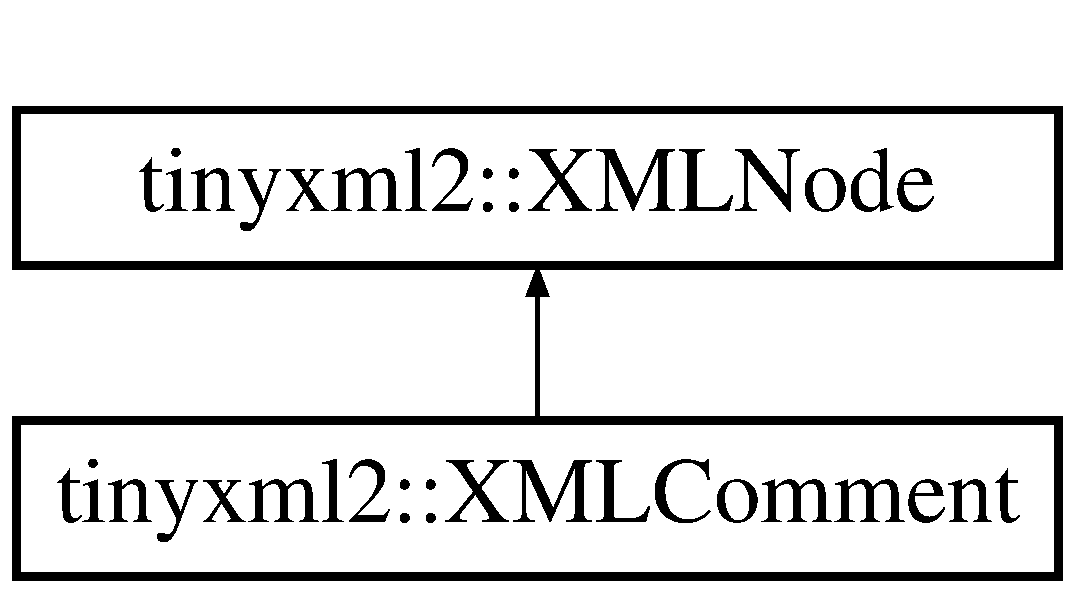
\includegraphics[height=2.000000cm]{classtinyxml2_1_1_x_m_l_comment}
\end{center}
\end{figure}
\subsection*{Public Member Functions}
\begin{DoxyCompactItemize}
\item 
virtual \hyperlink{classtinyxml2_1_1_x_m_l_comment}{X\+M\+L\+Comment} $\ast$ \hyperlink{classtinyxml2_1_1_x_m_l_comment_a8093e1dc8a34fa446d9dc3fde0e6c0ee}{To\+Comment} ()
\begin{DoxyCompactList}\small\item\em Safely cast to a Comment, or null. \end{DoxyCompactList}\item 
virtual const \hyperlink{classtinyxml2_1_1_x_m_l_comment}{X\+M\+L\+Comment} $\ast$ \hyperlink{classtinyxml2_1_1_x_m_l_comment_a8e60caf06d8e88876a94b81db026b85c}{To\+Comment} () const
\item 
virtual bool \hyperlink{classtinyxml2_1_1_x_m_l_comment_a27b37d16cea01b5329dfbbb4f9508e39}{Accept} (\hyperlink{classtinyxml2_1_1_x_m_l_visitor}{X\+M\+L\+Visitor} $\ast$visitor) const
\item 
virtual \hyperlink{classtinyxml2_1_1_x_m_l_node}{X\+M\+L\+Node} $\ast$ \hyperlink{classtinyxml2_1_1_x_m_l_comment_adf5b5c0319351dcc339df098d11e8fb2}{Shallow\+Clone} (\hyperlink{classtinyxml2_1_1_x_m_l_document}{X\+M\+L\+Document} $\ast$document) const
\item 
virtual bool \hyperlink{classtinyxml2_1_1_x_m_l_comment_a965d880a99d58dd915caa88dc37a9b51}{Shallow\+Equal} (const \hyperlink{classtinyxml2_1_1_x_m_l_node}{X\+M\+L\+Node} $\ast$compare) const
\end{DoxyCompactItemize}
\subsection*{Protected Member Functions}
\begin{DoxyCompactItemize}
\item 
\hyperlink{classtinyxml2_1_1_x_m_l_comment_ae6463adc3edd93a8e5a9b2b7e99cdf91}{X\+M\+L\+Comment} (\hyperlink{classtinyxml2_1_1_x_m_l_document}{X\+M\+L\+Document} $\ast$doc)
\item 
virtual \hyperlink{classtinyxml2_1_1_x_m_l_comment_ab592f69b47852455c1b32c5e31e453d0}{$\sim$\+X\+M\+L\+Comment} ()
\item 
char $\ast$ \hyperlink{classtinyxml2_1_1_x_m_l_comment_ae61ea28c1ba2e092ba4c63c088ce6474}{Parse\+Deep} (char $\ast$, \hyperlink{classtinyxml2_1_1_str_pair}{Str\+Pair} $\ast$end\+Tag, int $\ast$cur\+Line\+Num\+Ptr)
\end{DoxyCompactItemize}
\subsection*{Friends}
\begin{DoxyCompactItemize}
\item 
class \hyperlink{classtinyxml2_1_1_x_m_l_comment_a4eee3bda60c60a30e4e8cd4ea91c4c6e}{X\+M\+L\+Document}
\end{DoxyCompactItemize}
\subsection*{Additional Inherited Members}


\subsection{Detailed Description}
An X\+ML Comment. 

\subsection{Constructor \& Destructor Documentation}
\mbox{\Hypertarget{classtinyxml2_1_1_x_m_l_comment_ae6463adc3edd93a8e5a9b2b7e99cdf91}\label{classtinyxml2_1_1_x_m_l_comment_ae6463adc3edd93a8e5a9b2b7e99cdf91}} 
\index{tinyxml2\+::\+X\+M\+L\+Comment@{tinyxml2\+::\+X\+M\+L\+Comment}!X\+M\+L\+Comment@{X\+M\+L\+Comment}}
\index{X\+M\+L\+Comment@{X\+M\+L\+Comment}!tinyxml2\+::\+X\+M\+L\+Comment@{tinyxml2\+::\+X\+M\+L\+Comment}}
\subsubsection{\texorpdfstring{X\+M\+L\+Comment()}{XMLComment()}}
{\footnotesize\ttfamily tinyxml2\+::\+X\+M\+L\+Comment\+::\+X\+M\+L\+Comment (\begin{DoxyParamCaption}\item[{\hyperlink{classtinyxml2_1_1_x_m_l_document}{X\+M\+L\+Document} $\ast$}]{doc }\end{DoxyParamCaption})\hspace{0.3cm}{\ttfamily [protected]}}

\mbox{\Hypertarget{classtinyxml2_1_1_x_m_l_comment_ab592f69b47852455c1b32c5e31e453d0}\label{classtinyxml2_1_1_x_m_l_comment_ab592f69b47852455c1b32c5e31e453d0}} 
\index{tinyxml2\+::\+X\+M\+L\+Comment@{tinyxml2\+::\+X\+M\+L\+Comment}!````~X\+M\+L\+Comment@{$\sim$\+X\+M\+L\+Comment}}
\index{````~X\+M\+L\+Comment@{$\sim$\+X\+M\+L\+Comment}!tinyxml2\+::\+X\+M\+L\+Comment@{tinyxml2\+::\+X\+M\+L\+Comment}}
\subsubsection{\texorpdfstring{$\sim$\+X\+M\+L\+Comment()}{~XMLComment()}}
{\footnotesize\ttfamily tinyxml2\+::\+X\+M\+L\+Comment\+::$\sim$\+X\+M\+L\+Comment (\begin{DoxyParamCaption}{ }\end{DoxyParamCaption})\hspace{0.3cm}{\ttfamily [protected]}, {\ttfamily [virtual]}}



\subsection{Member Function Documentation}
\mbox{\Hypertarget{classtinyxml2_1_1_x_m_l_comment_a27b37d16cea01b5329dfbbb4f9508e39}\label{classtinyxml2_1_1_x_m_l_comment_a27b37d16cea01b5329dfbbb4f9508e39}} 
\index{tinyxml2\+::\+X\+M\+L\+Comment@{tinyxml2\+::\+X\+M\+L\+Comment}!Accept@{Accept}}
\index{Accept@{Accept}!tinyxml2\+::\+X\+M\+L\+Comment@{tinyxml2\+::\+X\+M\+L\+Comment}}
\subsubsection{\texorpdfstring{Accept()}{Accept()}}
{\footnotesize\ttfamily bool tinyxml2\+::\+X\+M\+L\+Comment\+::\+Accept (\begin{DoxyParamCaption}\item[{\hyperlink{classtinyxml2_1_1_x_m_l_visitor}{X\+M\+L\+Visitor} $\ast$}]{visitor }\end{DoxyParamCaption}) const\hspace{0.3cm}{\ttfamily [virtual]}}

Accept a hierarchical visit of the nodes in the Tiny\+X\+M\+L-\/2 D\+OM. Every node in the X\+ML tree will be conditionally visited and the host will be called back via the \hyperlink{classtinyxml2_1_1_x_m_l_visitor}{X\+M\+L\+Visitor} interface.

This is essentially a S\+AX interface for Tiny\+X\+M\+L-\/2. (Note however it doesn\textquotesingle{}t re-\/parse the X\+ML for the callbacks, so the performance of Tiny\+X\+M\+L-\/2 is unchanged by using this interface versus any other.)

The interface has been based on ideas from\+:


\begin{DoxyItemize}
\item \href{http://www.saxproject.org/}{\tt http\+://www.\+saxproject.\+org/}
\item \href{http://c2.com/cgi/wiki?HierarchicalVisitorPattern}{\tt http\+://c2.\+com/cgi/wiki?\+Hierarchical\+Visitor\+Pattern}
\end{DoxyItemize}

Which are both good references for \char`\"{}visiting\char`\"{}.

An example of using \hyperlink{classtinyxml2_1_1_x_m_l_comment_a27b37d16cea01b5329dfbbb4f9508e39}{Accept()}\+: \begin{DoxyVerb}XMLPrinter printer;
tinyxmlDoc.Accept( &printer );
const char* xmlcstr = printer.CStr();
\end{DoxyVerb}
 

Implements \hyperlink{classtinyxml2_1_1_x_m_l_node_a81e66df0a44c67a7af17f3b77a152785}{tinyxml2\+::\+X\+M\+L\+Node}.

\mbox{\Hypertarget{classtinyxml2_1_1_x_m_l_comment_ae61ea28c1ba2e092ba4c63c088ce6474}\label{classtinyxml2_1_1_x_m_l_comment_ae61ea28c1ba2e092ba4c63c088ce6474}} 
\index{tinyxml2\+::\+X\+M\+L\+Comment@{tinyxml2\+::\+X\+M\+L\+Comment}!Parse\+Deep@{Parse\+Deep}}
\index{Parse\+Deep@{Parse\+Deep}!tinyxml2\+::\+X\+M\+L\+Comment@{tinyxml2\+::\+X\+M\+L\+Comment}}
\subsubsection{\texorpdfstring{Parse\+Deep()}{ParseDeep()}}
{\footnotesize\ttfamily char $\ast$ tinyxml2\+::\+X\+M\+L\+Comment\+::\+Parse\+Deep (\begin{DoxyParamCaption}\item[{char $\ast$}]{p,  }\item[{\hyperlink{classtinyxml2_1_1_str_pair}{Str\+Pair} $\ast$}]{end\+Tag,  }\item[{int $\ast$}]{cur\+Line\+Num\+Ptr }\end{DoxyParamCaption})\hspace{0.3cm}{\ttfamily [protected]}, {\ttfamily [virtual]}}



Reimplemented from \hyperlink{classtinyxml2_1_1_x_m_l_node_a0afc27892998f31735f6225edb40a40d}{tinyxml2\+::\+X\+M\+L\+Node}.

\mbox{\Hypertarget{classtinyxml2_1_1_x_m_l_comment_adf5b5c0319351dcc339df098d11e8fb2}\label{classtinyxml2_1_1_x_m_l_comment_adf5b5c0319351dcc339df098d11e8fb2}} 
\index{tinyxml2\+::\+X\+M\+L\+Comment@{tinyxml2\+::\+X\+M\+L\+Comment}!Shallow\+Clone@{Shallow\+Clone}}
\index{Shallow\+Clone@{Shallow\+Clone}!tinyxml2\+::\+X\+M\+L\+Comment@{tinyxml2\+::\+X\+M\+L\+Comment}}
\subsubsection{\texorpdfstring{Shallow\+Clone()}{ShallowClone()}}
{\footnotesize\ttfamily \hyperlink{classtinyxml2_1_1_x_m_l_node}{X\+M\+L\+Node} $\ast$ tinyxml2\+::\+X\+M\+L\+Comment\+::\+Shallow\+Clone (\begin{DoxyParamCaption}\item[{\hyperlink{classtinyxml2_1_1_x_m_l_document}{X\+M\+L\+Document} $\ast$}]{document }\end{DoxyParamCaption}) const\hspace{0.3cm}{\ttfamily [virtual]}}

Make a copy of this node, but not its children. You may pass in a Document pointer that will be the owner of the new Node. If the \textquotesingle{}document\textquotesingle{} is null, then the node returned will be allocated from the current Document. (this-\/$>$\hyperlink{classtinyxml2_1_1_x_m_l_node_af343d1ef0b45c0020e62d784d7e67a68}{Get\+Document()})

Note\+: if called on a \hyperlink{classtinyxml2_1_1_x_m_l_document}{X\+M\+L\+Document}, this will return null. 

Implements \hyperlink{classtinyxml2_1_1_x_m_l_node_a8402cbd3129d20e9e6024bbcc0531283}{tinyxml2\+::\+X\+M\+L\+Node}.

\mbox{\Hypertarget{classtinyxml2_1_1_x_m_l_comment_a965d880a99d58dd915caa88dc37a9b51}\label{classtinyxml2_1_1_x_m_l_comment_a965d880a99d58dd915caa88dc37a9b51}} 
\index{tinyxml2\+::\+X\+M\+L\+Comment@{tinyxml2\+::\+X\+M\+L\+Comment}!Shallow\+Equal@{Shallow\+Equal}}
\index{Shallow\+Equal@{Shallow\+Equal}!tinyxml2\+::\+X\+M\+L\+Comment@{tinyxml2\+::\+X\+M\+L\+Comment}}
\subsubsection{\texorpdfstring{Shallow\+Equal()}{ShallowEqual()}}
{\footnotesize\ttfamily bool tinyxml2\+::\+X\+M\+L\+Comment\+::\+Shallow\+Equal (\begin{DoxyParamCaption}\item[{const \hyperlink{classtinyxml2_1_1_x_m_l_node}{X\+M\+L\+Node} $\ast$}]{compare }\end{DoxyParamCaption}) const\hspace{0.3cm}{\ttfamily [virtual]}}

Test if 2 nodes are the same, but don\textquotesingle{}t test children. The 2 nodes do not need to be in the same Document.

Note\+: if called on a \hyperlink{classtinyxml2_1_1_x_m_l_document}{X\+M\+L\+Document}, this will return false. 

Implements \hyperlink{classtinyxml2_1_1_x_m_l_node_a7ce18b751c3ea09eac292dca264f9226}{tinyxml2\+::\+X\+M\+L\+Node}.

\mbox{\Hypertarget{classtinyxml2_1_1_x_m_l_comment_a8093e1dc8a34fa446d9dc3fde0e6c0ee}\label{classtinyxml2_1_1_x_m_l_comment_a8093e1dc8a34fa446d9dc3fde0e6c0ee}} 
\index{tinyxml2\+::\+X\+M\+L\+Comment@{tinyxml2\+::\+X\+M\+L\+Comment}!To\+Comment@{To\+Comment}}
\index{To\+Comment@{To\+Comment}!tinyxml2\+::\+X\+M\+L\+Comment@{tinyxml2\+::\+X\+M\+L\+Comment}}
\subsubsection{\texorpdfstring{To\+Comment()}{ToComment()}\hspace{0.1cm}{\footnotesize\ttfamily [1/2]}}
{\footnotesize\ttfamily virtual \hyperlink{classtinyxml2_1_1_x_m_l_comment}{X\+M\+L\+Comment}$\ast$ tinyxml2\+::\+X\+M\+L\+Comment\+::\+To\+Comment (\begin{DoxyParamCaption}{ }\end{DoxyParamCaption})\hspace{0.3cm}{\ttfamily [inline]}, {\ttfamily [virtual]}}



Safely cast to a Comment, or null. 



Reimplemented from \hyperlink{classtinyxml2_1_1_x_m_l_node_aff47671055aa99840a1c1ebd661e63e3}{tinyxml2\+::\+X\+M\+L\+Node}.

\mbox{\Hypertarget{classtinyxml2_1_1_x_m_l_comment_a8e60caf06d8e88876a94b81db026b85c}\label{classtinyxml2_1_1_x_m_l_comment_a8e60caf06d8e88876a94b81db026b85c}} 
\index{tinyxml2\+::\+X\+M\+L\+Comment@{tinyxml2\+::\+X\+M\+L\+Comment}!To\+Comment@{To\+Comment}}
\index{To\+Comment@{To\+Comment}!tinyxml2\+::\+X\+M\+L\+Comment@{tinyxml2\+::\+X\+M\+L\+Comment}}
\subsubsection{\texorpdfstring{To\+Comment()}{ToComment()}\hspace{0.1cm}{\footnotesize\ttfamily [2/2]}}
{\footnotesize\ttfamily virtual const \hyperlink{classtinyxml2_1_1_x_m_l_comment}{X\+M\+L\+Comment}$\ast$ tinyxml2\+::\+X\+M\+L\+Comment\+::\+To\+Comment (\begin{DoxyParamCaption}{ }\end{DoxyParamCaption}) const\hspace{0.3cm}{\ttfamily [inline]}, {\ttfamily [virtual]}}



Reimplemented from \hyperlink{classtinyxml2_1_1_x_m_l_node_a6a53bb83faf5c0ccc95b6cf74dba0025}{tinyxml2\+::\+X\+M\+L\+Node}.



\subsection{Friends And Related Function Documentation}
\mbox{\Hypertarget{classtinyxml2_1_1_x_m_l_comment_a4eee3bda60c60a30e4e8cd4ea91c4c6e}\label{classtinyxml2_1_1_x_m_l_comment_a4eee3bda60c60a30e4e8cd4ea91c4c6e}} 
\index{tinyxml2\+::\+X\+M\+L\+Comment@{tinyxml2\+::\+X\+M\+L\+Comment}!X\+M\+L\+Document@{X\+M\+L\+Document}}
\index{X\+M\+L\+Document@{X\+M\+L\+Document}!tinyxml2\+::\+X\+M\+L\+Comment@{tinyxml2\+::\+X\+M\+L\+Comment}}
\subsubsection{\texorpdfstring{X\+M\+L\+Document}{XMLDocument}}
{\footnotesize\ttfamily friend class \hyperlink{classtinyxml2_1_1_x_m_l_document}{X\+M\+L\+Document}\hspace{0.3cm}{\ttfamily [friend]}}



The documentation for this class was generated from the following files\+:\begin{DoxyCompactItemize}
\item 
\hyperlink{tinyxml2_8h}{tinyxml2.\+h}\item 
\hyperlink{tinyxml2_8cpp}{tinyxml2.\+cpp}\end{DoxyCompactItemize}

\hypertarget{classtinyxml2_1_1_x_m_l_const_handle}{}\section{tinyxml2\+:\+:X\+M\+L\+Const\+Handle Class Reference}
\label{classtinyxml2_1_1_x_m_l_const_handle}\index{tinyxml2\+::\+X\+M\+L\+Const\+Handle@{tinyxml2\+::\+X\+M\+L\+Const\+Handle}}


{\ttfamily \#include $<$tinyxml2.\+h$>$}

\subsection*{Public Member Functions}
\begin{DoxyCompactItemize}
\item 
\hyperlink{classtinyxml2_1_1_x_m_l_const_handle_a098bda71fa11d7c74ccddab59d5dd534}{X\+M\+L\+Const\+Handle} (const \hyperlink{classtinyxml2_1_1_x_m_l_node}{X\+M\+L\+Node} $\ast$node)
\item 
\hyperlink{classtinyxml2_1_1_x_m_l_const_handle_a8420a0c4720637e0529e78c2e22f2b0b}{X\+M\+L\+Const\+Handle} (const \hyperlink{classtinyxml2_1_1_x_m_l_node}{X\+M\+L\+Node} \&node)
\item 
\hyperlink{classtinyxml2_1_1_x_m_l_const_handle_a639317ad315ff24f4ef0dc69312d7303}{X\+M\+L\+Const\+Handle} (const \hyperlink{classtinyxml2_1_1_x_m_l_const_handle}{X\+M\+L\+Const\+Handle} \&ref)
\item 
\hyperlink{classtinyxml2_1_1_x_m_l_const_handle}{X\+M\+L\+Const\+Handle} \& \hyperlink{classtinyxml2_1_1_x_m_l_const_handle_a2d74c91df1ff9aa5f9b57e3dceddbf94}{operator=} (const \hyperlink{classtinyxml2_1_1_x_m_l_const_handle}{X\+M\+L\+Const\+Handle} \&ref)
\item 
const \hyperlink{classtinyxml2_1_1_x_m_l_const_handle}{X\+M\+L\+Const\+Handle} \hyperlink{classtinyxml2_1_1_x_m_l_const_handle_aef06bd16cb308652a32b864b0a743136}{First\+Child} () const
\item 
const \hyperlink{classtinyxml2_1_1_x_m_l_const_handle}{X\+M\+L\+Const\+Handle} \hyperlink{classtinyxml2_1_1_x_m_l_const_handle_ac747db472ffc55c5af2e82ffec813640}{First\+Child\+Element} (const char $\ast$name=0) const
\item 
const \hyperlink{classtinyxml2_1_1_x_m_l_const_handle}{X\+M\+L\+Const\+Handle} \hyperlink{classtinyxml2_1_1_x_m_l_const_handle_a908436124990f3d7b35cb7df20d31d9e}{Last\+Child} () const
\item 
const \hyperlink{classtinyxml2_1_1_x_m_l_const_handle}{X\+M\+L\+Const\+Handle} \hyperlink{classtinyxml2_1_1_x_m_l_const_handle_a9de0475ec42bd50c0e64624a250ba5b2}{Last\+Child\+Element} (const char $\ast$name=0) const
\item 
const \hyperlink{classtinyxml2_1_1_x_m_l_const_handle}{X\+M\+L\+Const\+Handle} \hyperlink{classtinyxml2_1_1_x_m_l_const_handle_acf68cc7930e4ac883e0c7e16ef2fbb66}{Previous\+Sibling} () const
\item 
const \hyperlink{classtinyxml2_1_1_x_m_l_const_handle}{X\+M\+L\+Const\+Handle} \hyperlink{classtinyxml2_1_1_x_m_l_const_handle_aef99308659f2617299ac29980769a91e}{Previous\+Sibling\+Element} (const char $\ast$name=0) const
\item 
const \hyperlink{classtinyxml2_1_1_x_m_l_const_handle}{X\+M\+L\+Const\+Handle} \hyperlink{classtinyxml2_1_1_x_m_l_const_handle_aec3710e455f41014026ef17fbbb0efb3}{Next\+Sibling} () const
\item 
const \hyperlink{classtinyxml2_1_1_x_m_l_const_handle}{X\+M\+L\+Const\+Handle} \hyperlink{classtinyxml2_1_1_x_m_l_const_handle_a3c9e6b48b02d3d5232e1e8780753d8a5}{Next\+Sibling\+Element} (const char $\ast$name=0) const
\item 
const \hyperlink{classtinyxml2_1_1_x_m_l_node}{X\+M\+L\+Node} $\ast$ \hyperlink{classtinyxml2_1_1_x_m_l_const_handle_a61812760cb08bc1b050e65b73a08457b}{To\+Node} () const
\item 
const \hyperlink{classtinyxml2_1_1_x_m_l_element}{X\+M\+L\+Element} $\ast$ \hyperlink{classtinyxml2_1_1_x_m_l_const_handle_a4dba53c6e201d412e915620feaaa56f3}{To\+Element} () const
\item 
const \hyperlink{classtinyxml2_1_1_x_m_l_text}{X\+M\+L\+Text} $\ast$ \hyperlink{classtinyxml2_1_1_x_m_l_const_handle_a80e24d90d476005aa35602a665358e2d}{To\+Text} () const
\item 
const \hyperlink{classtinyxml2_1_1_x_m_l_unknown}{X\+M\+L\+Unknown} $\ast$ \hyperlink{classtinyxml2_1_1_x_m_l_const_handle_a4395e5feaba7b456a81ca274880ea3d3}{To\+Unknown} () const
\item 
const \hyperlink{classtinyxml2_1_1_x_m_l_declaration}{X\+M\+L\+Declaration} $\ast$ \hyperlink{classtinyxml2_1_1_x_m_l_const_handle_a55e306d105fa80d626041e4d3b77b716}{To\+Declaration} () const
\end{DoxyCompactItemize}


\subsection{Detailed Description}
A variant of the \hyperlink{classtinyxml2_1_1_x_m_l_handle}{X\+M\+L\+Handle} class for working with const X\+M\+L\+Nodes and Documents. It is the same in all regards, except for the \textquotesingle{}const\textquotesingle{} qualifiers. See \hyperlink{classtinyxml2_1_1_x_m_l_handle}{X\+M\+L\+Handle} for A\+PI. 

\subsection{Constructor \& Destructor Documentation}
\mbox{\Hypertarget{classtinyxml2_1_1_x_m_l_const_handle_a098bda71fa11d7c74ccddab59d5dd534}\label{classtinyxml2_1_1_x_m_l_const_handle_a098bda71fa11d7c74ccddab59d5dd534}} 
\index{tinyxml2\+::\+X\+M\+L\+Const\+Handle@{tinyxml2\+::\+X\+M\+L\+Const\+Handle}!X\+M\+L\+Const\+Handle@{X\+M\+L\+Const\+Handle}}
\index{X\+M\+L\+Const\+Handle@{X\+M\+L\+Const\+Handle}!tinyxml2\+::\+X\+M\+L\+Const\+Handle@{tinyxml2\+::\+X\+M\+L\+Const\+Handle}}
\subsubsection{\texorpdfstring{X\+M\+L\+Const\+Handle()}{XMLConstHandle()}\hspace{0.1cm}{\footnotesize\ttfamily [1/3]}}
{\footnotesize\ttfamily tinyxml2\+::\+X\+M\+L\+Const\+Handle\+::\+X\+M\+L\+Const\+Handle (\begin{DoxyParamCaption}\item[{const \hyperlink{classtinyxml2_1_1_x_m_l_node}{X\+M\+L\+Node} $\ast$}]{node }\end{DoxyParamCaption})\hspace{0.3cm}{\ttfamily [inline]}}

\mbox{\Hypertarget{classtinyxml2_1_1_x_m_l_const_handle_a8420a0c4720637e0529e78c2e22f2b0b}\label{classtinyxml2_1_1_x_m_l_const_handle_a8420a0c4720637e0529e78c2e22f2b0b}} 
\index{tinyxml2\+::\+X\+M\+L\+Const\+Handle@{tinyxml2\+::\+X\+M\+L\+Const\+Handle}!X\+M\+L\+Const\+Handle@{X\+M\+L\+Const\+Handle}}
\index{X\+M\+L\+Const\+Handle@{X\+M\+L\+Const\+Handle}!tinyxml2\+::\+X\+M\+L\+Const\+Handle@{tinyxml2\+::\+X\+M\+L\+Const\+Handle}}
\subsubsection{\texorpdfstring{X\+M\+L\+Const\+Handle()}{XMLConstHandle()}\hspace{0.1cm}{\footnotesize\ttfamily [2/3]}}
{\footnotesize\ttfamily tinyxml2\+::\+X\+M\+L\+Const\+Handle\+::\+X\+M\+L\+Const\+Handle (\begin{DoxyParamCaption}\item[{const \hyperlink{classtinyxml2_1_1_x_m_l_node}{X\+M\+L\+Node} \&}]{node }\end{DoxyParamCaption})\hspace{0.3cm}{\ttfamily [inline]}}

\mbox{\Hypertarget{classtinyxml2_1_1_x_m_l_const_handle_a639317ad315ff24f4ef0dc69312d7303}\label{classtinyxml2_1_1_x_m_l_const_handle_a639317ad315ff24f4ef0dc69312d7303}} 
\index{tinyxml2\+::\+X\+M\+L\+Const\+Handle@{tinyxml2\+::\+X\+M\+L\+Const\+Handle}!X\+M\+L\+Const\+Handle@{X\+M\+L\+Const\+Handle}}
\index{X\+M\+L\+Const\+Handle@{X\+M\+L\+Const\+Handle}!tinyxml2\+::\+X\+M\+L\+Const\+Handle@{tinyxml2\+::\+X\+M\+L\+Const\+Handle}}
\subsubsection{\texorpdfstring{X\+M\+L\+Const\+Handle()}{XMLConstHandle()}\hspace{0.1cm}{\footnotesize\ttfamily [3/3]}}
{\footnotesize\ttfamily tinyxml2\+::\+X\+M\+L\+Const\+Handle\+::\+X\+M\+L\+Const\+Handle (\begin{DoxyParamCaption}\item[{const \hyperlink{classtinyxml2_1_1_x_m_l_const_handle}{X\+M\+L\+Const\+Handle} \&}]{ref }\end{DoxyParamCaption})\hspace{0.3cm}{\ttfamily [inline]}}



\subsection{Member Function Documentation}
\mbox{\Hypertarget{classtinyxml2_1_1_x_m_l_const_handle_aef06bd16cb308652a32b864b0a743136}\label{classtinyxml2_1_1_x_m_l_const_handle_aef06bd16cb308652a32b864b0a743136}} 
\index{tinyxml2\+::\+X\+M\+L\+Const\+Handle@{tinyxml2\+::\+X\+M\+L\+Const\+Handle}!First\+Child@{First\+Child}}
\index{First\+Child@{First\+Child}!tinyxml2\+::\+X\+M\+L\+Const\+Handle@{tinyxml2\+::\+X\+M\+L\+Const\+Handle}}
\subsubsection{\texorpdfstring{First\+Child()}{FirstChild()}}
{\footnotesize\ttfamily const \hyperlink{classtinyxml2_1_1_x_m_l_const_handle}{X\+M\+L\+Const\+Handle} tinyxml2\+::\+X\+M\+L\+Const\+Handle\+::\+First\+Child (\begin{DoxyParamCaption}{ }\end{DoxyParamCaption}) const\hspace{0.3cm}{\ttfamily [inline]}}

\mbox{\Hypertarget{classtinyxml2_1_1_x_m_l_const_handle_ac747db472ffc55c5af2e82ffec813640}\label{classtinyxml2_1_1_x_m_l_const_handle_ac747db472ffc55c5af2e82ffec813640}} 
\index{tinyxml2\+::\+X\+M\+L\+Const\+Handle@{tinyxml2\+::\+X\+M\+L\+Const\+Handle}!First\+Child\+Element@{First\+Child\+Element}}
\index{First\+Child\+Element@{First\+Child\+Element}!tinyxml2\+::\+X\+M\+L\+Const\+Handle@{tinyxml2\+::\+X\+M\+L\+Const\+Handle}}
\subsubsection{\texorpdfstring{First\+Child\+Element()}{FirstChildElement()}}
{\footnotesize\ttfamily const \hyperlink{classtinyxml2_1_1_x_m_l_const_handle}{X\+M\+L\+Const\+Handle} tinyxml2\+::\+X\+M\+L\+Const\+Handle\+::\+First\+Child\+Element (\begin{DoxyParamCaption}\item[{const char $\ast$}]{name = {\ttfamily 0} }\end{DoxyParamCaption}) const\hspace{0.3cm}{\ttfamily [inline]}}

\mbox{\Hypertarget{classtinyxml2_1_1_x_m_l_const_handle_a908436124990f3d7b35cb7df20d31d9e}\label{classtinyxml2_1_1_x_m_l_const_handle_a908436124990f3d7b35cb7df20d31d9e}} 
\index{tinyxml2\+::\+X\+M\+L\+Const\+Handle@{tinyxml2\+::\+X\+M\+L\+Const\+Handle}!Last\+Child@{Last\+Child}}
\index{Last\+Child@{Last\+Child}!tinyxml2\+::\+X\+M\+L\+Const\+Handle@{tinyxml2\+::\+X\+M\+L\+Const\+Handle}}
\subsubsection{\texorpdfstring{Last\+Child()}{LastChild()}}
{\footnotesize\ttfamily const \hyperlink{classtinyxml2_1_1_x_m_l_const_handle}{X\+M\+L\+Const\+Handle} tinyxml2\+::\+X\+M\+L\+Const\+Handle\+::\+Last\+Child (\begin{DoxyParamCaption}{ }\end{DoxyParamCaption}) const\hspace{0.3cm}{\ttfamily [inline]}}

\mbox{\Hypertarget{classtinyxml2_1_1_x_m_l_const_handle_a9de0475ec42bd50c0e64624a250ba5b2}\label{classtinyxml2_1_1_x_m_l_const_handle_a9de0475ec42bd50c0e64624a250ba5b2}} 
\index{tinyxml2\+::\+X\+M\+L\+Const\+Handle@{tinyxml2\+::\+X\+M\+L\+Const\+Handle}!Last\+Child\+Element@{Last\+Child\+Element}}
\index{Last\+Child\+Element@{Last\+Child\+Element}!tinyxml2\+::\+X\+M\+L\+Const\+Handle@{tinyxml2\+::\+X\+M\+L\+Const\+Handle}}
\subsubsection{\texorpdfstring{Last\+Child\+Element()}{LastChildElement()}}
{\footnotesize\ttfamily const \hyperlink{classtinyxml2_1_1_x_m_l_const_handle}{X\+M\+L\+Const\+Handle} tinyxml2\+::\+X\+M\+L\+Const\+Handle\+::\+Last\+Child\+Element (\begin{DoxyParamCaption}\item[{const char $\ast$}]{name = {\ttfamily 0} }\end{DoxyParamCaption}) const\hspace{0.3cm}{\ttfamily [inline]}}

\mbox{\Hypertarget{classtinyxml2_1_1_x_m_l_const_handle_aec3710e455f41014026ef17fbbb0efb3}\label{classtinyxml2_1_1_x_m_l_const_handle_aec3710e455f41014026ef17fbbb0efb3}} 
\index{tinyxml2\+::\+X\+M\+L\+Const\+Handle@{tinyxml2\+::\+X\+M\+L\+Const\+Handle}!Next\+Sibling@{Next\+Sibling}}
\index{Next\+Sibling@{Next\+Sibling}!tinyxml2\+::\+X\+M\+L\+Const\+Handle@{tinyxml2\+::\+X\+M\+L\+Const\+Handle}}
\subsubsection{\texorpdfstring{Next\+Sibling()}{NextSibling()}}
{\footnotesize\ttfamily const \hyperlink{classtinyxml2_1_1_x_m_l_const_handle}{X\+M\+L\+Const\+Handle} tinyxml2\+::\+X\+M\+L\+Const\+Handle\+::\+Next\+Sibling (\begin{DoxyParamCaption}{ }\end{DoxyParamCaption}) const\hspace{0.3cm}{\ttfamily [inline]}}

\mbox{\Hypertarget{classtinyxml2_1_1_x_m_l_const_handle_a3c9e6b48b02d3d5232e1e8780753d8a5}\label{classtinyxml2_1_1_x_m_l_const_handle_a3c9e6b48b02d3d5232e1e8780753d8a5}} 
\index{tinyxml2\+::\+X\+M\+L\+Const\+Handle@{tinyxml2\+::\+X\+M\+L\+Const\+Handle}!Next\+Sibling\+Element@{Next\+Sibling\+Element}}
\index{Next\+Sibling\+Element@{Next\+Sibling\+Element}!tinyxml2\+::\+X\+M\+L\+Const\+Handle@{tinyxml2\+::\+X\+M\+L\+Const\+Handle}}
\subsubsection{\texorpdfstring{Next\+Sibling\+Element()}{NextSiblingElement()}}
{\footnotesize\ttfamily const \hyperlink{classtinyxml2_1_1_x_m_l_const_handle}{X\+M\+L\+Const\+Handle} tinyxml2\+::\+X\+M\+L\+Const\+Handle\+::\+Next\+Sibling\+Element (\begin{DoxyParamCaption}\item[{const char $\ast$}]{name = {\ttfamily 0} }\end{DoxyParamCaption}) const\hspace{0.3cm}{\ttfamily [inline]}}

\mbox{\Hypertarget{classtinyxml2_1_1_x_m_l_const_handle_a2d74c91df1ff9aa5f9b57e3dceddbf94}\label{classtinyxml2_1_1_x_m_l_const_handle_a2d74c91df1ff9aa5f9b57e3dceddbf94}} 
\index{tinyxml2\+::\+X\+M\+L\+Const\+Handle@{tinyxml2\+::\+X\+M\+L\+Const\+Handle}!operator=@{operator=}}
\index{operator=@{operator=}!tinyxml2\+::\+X\+M\+L\+Const\+Handle@{tinyxml2\+::\+X\+M\+L\+Const\+Handle}}
\subsubsection{\texorpdfstring{operator=()}{operator=()}}
{\footnotesize\ttfamily \hyperlink{classtinyxml2_1_1_x_m_l_const_handle}{X\+M\+L\+Const\+Handle}\& tinyxml2\+::\+X\+M\+L\+Const\+Handle\+::operator= (\begin{DoxyParamCaption}\item[{const \hyperlink{classtinyxml2_1_1_x_m_l_const_handle}{X\+M\+L\+Const\+Handle} \&}]{ref }\end{DoxyParamCaption})\hspace{0.3cm}{\ttfamily [inline]}}

\mbox{\Hypertarget{classtinyxml2_1_1_x_m_l_const_handle_acf68cc7930e4ac883e0c7e16ef2fbb66}\label{classtinyxml2_1_1_x_m_l_const_handle_acf68cc7930e4ac883e0c7e16ef2fbb66}} 
\index{tinyxml2\+::\+X\+M\+L\+Const\+Handle@{tinyxml2\+::\+X\+M\+L\+Const\+Handle}!Previous\+Sibling@{Previous\+Sibling}}
\index{Previous\+Sibling@{Previous\+Sibling}!tinyxml2\+::\+X\+M\+L\+Const\+Handle@{tinyxml2\+::\+X\+M\+L\+Const\+Handle}}
\subsubsection{\texorpdfstring{Previous\+Sibling()}{PreviousSibling()}}
{\footnotesize\ttfamily const \hyperlink{classtinyxml2_1_1_x_m_l_const_handle}{X\+M\+L\+Const\+Handle} tinyxml2\+::\+X\+M\+L\+Const\+Handle\+::\+Previous\+Sibling (\begin{DoxyParamCaption}{ }\end{DoxyParamCaption}) const\hspace{0.3cm}{\ttfamily [inline]}}

\mbox{\Hypertarget{classtinyxml2_1_1_x_m_l_const_handle_aef99308659f2617299ac29980769a91e}\label{classtinyxml2_1_1_x_m_l_const_handle_aef99308659f2617299ac29980769a91e}} 
\index{tinyxml2\+::\+X\+M\+L\+Const\+Handle@{tinyxml2\+::\+X\+M\+L\+Const\+Handle}!Previous\+Sibling\+Element@{Previous\+Sibling\+Element}}
\index{Previous\+Sibling\+Element@{Previous\+Sibling\+Element}!tinyxml2\+::\+X\+M\+L\+Const\+Handle@{tinyxml2\+::\+X\+M\+L\+Const\+Handle}}
\subsubsection{\texorpdfstring{Previous\+Sibling\+Element()}{PreviousSiblingElement()}}
{\footnotesize\ttfamily const \hyperlink{classtinyxml2_1_1_x_m_l_const_handle}{X\+M\+L\+Const\+Handle} tinyxml2\+::\+X\+M\+L\+Const\+Handle\+::\+Previous\+Sibling\+Element (\begin{DoxyParamCaption}\item[{const char $\ast$}]{name = {\ttfamily 0} }\end{DoxyParamCaption}) const\hspace{0.3cm}{\ttfamily [inline]}}

\mbox{\Hypertarget{classtinyxml2_1_1_x_m_l_const_handle_a55e306d105fa80d626041e4d3b77b716}\label{classtinyxml2_1_1_x_m_l_const_handle_a55e306d105fa80d626041e4d3b77b716}} 
\index{tinyxml2\+::\+X\+M\+L\+Const\+Handle@{tinyxml2\+::\+X\+M\+L\+Const\+Handle}!To\+Declaration@{To\+Declaration}}
\index{To\+Declaration@{To\+Declaration}!tinyxml2\+::\+X\+M\+L\+Const\+Handle@{tinyxml2\+::\+X\+M\+L\+Const\+Handle}}
\subsubsection{\texorpdfstring{To\+Declaration()}{ToDeclaration()}}
{\footnotesize\ttfamily const \hyperlink{classtinyxml2_1_1_x_m_l_declaration}{X\+M\+L\+Declaration}$\ast$ tinyxml2\+::\+X\+M\+L\+Const\+Handle\+::\+To\+Declaration (\begin{DoxyParamCaption}{ }\end{DoxyParamCaption}) const\hspace{0.3cm}{\ttfamily [inline]}}

\mbox{\Hypertarget{classtinyxml2_1_1_x_m_l_const_handle_a4dba53c6e201d412e915620feaaa56f3}\label{classtinyxml2_1_1_x_m_l_const_handle_a4dba53c6e201d412e915620feaaa56f3}} 
\index{tinyxml2\+::\+X\+M\+L\+Const\+Handle@{tinyxml2\+::\+X\+M\+L\+Const\+Handle}!To\+Element@{To\+Element}}
\index{To\+Element@{To\+Element}!tinyxml2\+::\+X\+M\+L\+Const\+Handle@{tinyxml2\+::\+X\+M\+L\+Const\+Handle}}
\subsubsection{\texorpdfstring{To\+Element()}{ToElement()}}
{\footnotesize\ttfamily const \hyperlink{classtinyxml2_1_1_x_m_l_element}{X\+M\+L\+Element}$\ast$ tinyxml2\+::\+X\+M\+L\+Const\+Handle\+::\+To\+Element (\begin{DoxyParamCaption}{ }\end{DoxyParamCaption}) const\hspace{0.3cm}{\ttfamily [inline]}}

\mbox{\Hypertarget{classtinyxml2_1_1_x_m_l_const_handle_a61812760cb08bc1b050e65b73a08457b}\label{classtinyxml2_1_1_x_m_l_const_handle_a61812760cb08bc1b050e65b73a08457b}} 
\index{tinyxml2\+::\+X\+M\+L\+Const\+Handle@{tinyxml2\+::\+X\+M\+L\+Const\+Handle}!To\+Node@{To\+Node}}
\index{To\+Node@{To\+Node}!tinyxml2\+::\+X\+M\+L\+Const\+Handle@{tinyxml2\+::\+X\+M\+L\+Const\+Handle}}
\subsubsection{\texorpdfstring{To\+Node()}{ToNode()}}
{\footnotesize\ttfamily const \hyperlink{classtinyxml2_1_1_x_m_l_node}{X\+M\+L\+Node}$\ast$ tinyxml2\+::\+X\+M\+L\+Const\+Handle\+::\+To\+Node (\begin{DoxyParamCaption}{ }\end{DoxyParamCaption}) const\hspace{0.3cm}{\ttfamily [inline]}}

\mbox{\Hypertarget{classtinyxml2_1_1_x_m_l_const_handle_a80e24d90d476005aa35602a665358e2d}\label{classtinyxml2_1_1_x_m_l_const_handle_a80e24d90d476005aa35602a665358e2d}} 
\index{tinyxml2\+::\+X\+M\+L\+Const\+Handle@{tinyxml2\+::\+X\+M\+L\+Const\+Handle}!To\+Text@{To\+Text}}
\index{To\+Text@{To\+Text}!tinyxml2\+::\+X\+M\+L\+Const\+Handle@{tinyxml2\+::\+X\+M\+L\+Const\+Handle}}
\subsubsection{\texorpdfstring{To\+Text()}{ToText()}}
{\footnotesize\ttfamily const \hyperlink{classtinyxml2_1_1_x_m_l_text}{X\+M\+L\+Text}$\ast$ tinyxml2\+::\+X\+M\+L\+Const\+Handle\+::\+To\+Text (\begin{DoxyParamCaption}{ }\end{DoxyParamCaption}) const\hspace{0.3cm}{\ttfamily [inline]}}

\mbox{\Hypertarget{classtinyxml2_1_1_x_m_l_const_handle_a4395e5feaba7b456a81ca274880ea3d3}\label{classtinyxml2_1_1_x_m_l_const_handle_a4395e5feaba7b456a81ca274880ea3d3}} 
\index{tinyxml2\+::\+X\+M\+L\+Const\+Handle@{tinyxml2\+::\+X\+M\+L\+Const\+Handle}!To\+Unknown@{To\+Unknown}}
\index{To\+Unknown@{To\+Unknown}!tinyxml2\+::\+X\+M\+L\+Const\+Handle@{tinyxml2\+::\+X\+M\+L\+Const\+Handle}}
\subsubsection{\texorpdfstring{To\+Unknown()}{ToUnknown()}}
{\footnotesize\ttfamily const \hyperlink{classtinyxml2_1_1_x_m_l_unknown}{X\+M\+L\+Unknown}$\ast$ tinyxml2\+::\+X\+M\+L\+Const\+Handle\+::\+To\+Unknown (\begin{DoxyParamCaption}{ }\end{DoxyParamCaption}) const\hspace{0.3cm}{\ttfamily [inline]}}



The documentation for this class was generated from the following file\+:\begin{DoxyCompactItemize}
\item 
\hyperlink{tinyxml2_8h}{tinyxml2.\+h}\end{DoxyCompactItemize}

\hypertarget{classtinyxml2_1_1_x_m_l_declaration}{}\section{tinyxml2\+:\+:X\+M\+L\+Declaration Class Reference}
\label{classtinyxml2_1_1_x_m_l_declaration}\index{tinyxml2\+::\+X\+M\+L\+Declaration@{tinyxml2\+::\+X\+M\+L\+Declaration}}


{\ttfamily \#include $<$tinyxml2.\+h$>$}

Inheritance diagram for tinyxml2\+:\+:X\+M\+L\+Declaration\+:\begin{figure}[H]
\begin{center}
\leavevmode
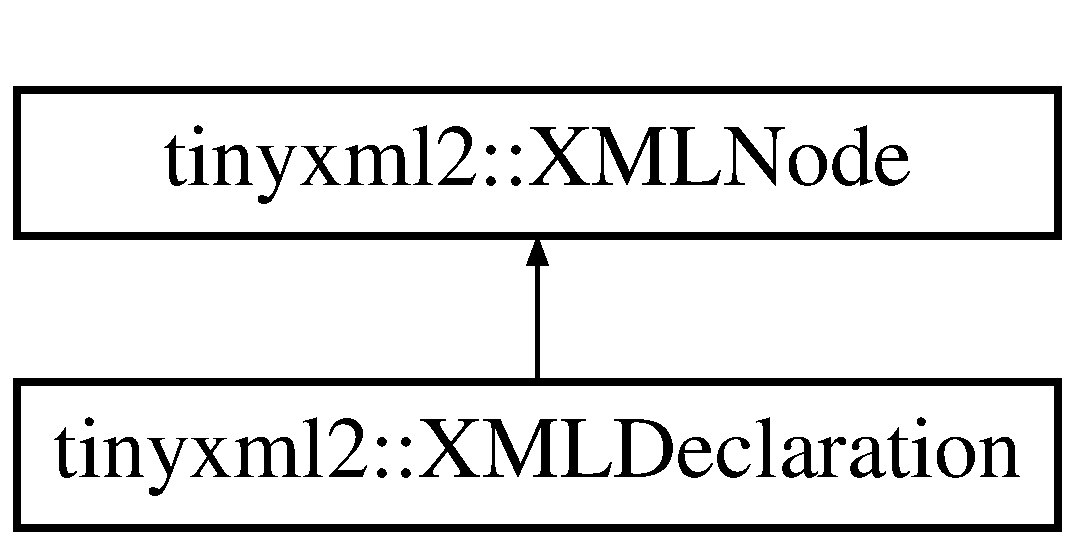
\includegraphics[height=2.000000cm]{classtinyxml2_1_1_x_m_l_declaration}
\end{center}
\end{figure}
\subsection*{Public Member Functions}
\begin{DoxyCompactItemize}
\item 
virtual \hyperlink{classtinyxml2_1_1_x_m_l_declaration}{X\+M\+L\+Declaration} $\ast$ \hyperlink{classtinyxml2_1_1_x_m_l_declaration_a159d8ac45865215e88059ea1e5b52fc5}{To\+Declaration} ()
\begin{DoxyCompactList}\small\item\em Safely cast to a Declaration, or null. \end{DoxyCompactList}\item 
virtual const \hyperlink{classtinyxml2_1_1_x_m_l_declaration}{X\+M\+L\+Declaration} $\ast$ \hyperlink{classtinyxml2_1_1_x_m_l_declaration_aa20c3315b18c3b88830dccf5c493259b}{To\+Declaration} () const
\item 
virtual bool \hyperlink{classtinyxml2_1_1_x_m_l_declaration_acf47629d9fc08ed6f1c164a97bcf794b}{Accept} (\hyperlink{classtinyxml2_1_1_x_m_l_visitor}{X\+M\+L\+Visitor} $\ast$visitor) const
\item 
virtual \hyperlink{classtinyxml2_1_1_x_m_l_node}{X\+M\+L\+Node} $\ast$ \hyperlink{classtinyxml2_1_1_x_m_l_declaration_ad9d60e6d2df75c13eb6bf7319985b747}{Shallow\+Clone} (\hyperlink{classtinyxml2_1_1_x_m_l_document}{X\+M\+L\+Document} $\ast$document) const
\item 
virtual bool \hyperlink{classtinyxml2_1_1_x_m_l_declaration_ae8b4d3a399857029f36c322b0801b69c}{Shallow\+Equal} (const \hyperlink{classtinyxml2_1_1_x_m_l_node}{X\+M\+L\+Node} $\ast$compare) const
\end{DoxyCompactItemize}
\subsection*{Protected Member Functions}
\begin{DoxyCompactItemize}
\item 
\hyperlink{classtinyxml2_1_1_x_m_l_declaration_aef9586f2ce5df5feba74dde49a242b06}{X\+M\+L\+Declaration} (\hyperlink{classtinyxml2_1_1_x_m_l_document}{X\+M\+L\+Document} $\ast$doc)
\item 
virtual \hyperlink{classtinyxml2_1_1_x_m_l_declaration_ab93d5bf4f5d58b4144963cf739cf6dcc}{$\sim$\+X\+M\+L\+Declaration} ()
\item 
char $\ast$ \hyperlink{classtinyxml2_1_1_x_m_l_declaration_a9a74a7d55c045d2d183878aaca0082dc}{Parse\+Deep} (char $\ast$, \hyperlink{classtinyxml2_1_1_str_pair}{Str\+Pair} $\ast$end\+Tag, int $\ast$cur\+Line\+Num\+Ptr)
\end{DoxyCompactItemize}
\subsection*{Friends}
\begin{DoxyCompactItemize}
\item 
class \hyperlink{classtinyxml2_1_1_x_m_l_declaration_a4eee3bda60c60a30e4e8cd4ea91c4c6e}{X\+M\+L\+Document}
\end{DoxyCompactItemize}
\subsection*{Additional Inherited Members}


\subsection{Detailed Description}
In correct X\+ML the declaration is the first entry in the file. \begin{DoxyVerb}<?xml version="1.0" standalone="yes"?>
\end{DoxyVerb}


Tiny\+X\+M\+L-\/2 will happily read or write files without a declaration, however.

The text of the declaration isn\textquotesingle{}t interpreted. It is parsed and written as a string. 

\subsection{Constructor \& Destructor Documentation}
\mbox{\Hypertarget{classtinyxml2_1_1_x_m_l_declaration_aef9586f2ce5df5feba74dde49a242b06}\label{classtinyxml2_1_1_x_m_l_declaration_aef9586f2ce5df5feba74dde49a242b06}} 
\index{tinyxml2\+::\+X\+M\+L\+Declaration@{tinyxml2\+::\+X\+M\+L\+Declaration}!X\+M\+L\+Declaration@{X\+M\+L\+Declaration}}
\index{X\+M\+L\+Declaration@{X\+M\+L\+Declaration}!tinyxml2\+::\+X\+M\+L\+Declaration@{tinyxml2\+::\+X\+M\+L\+Declaration}}
\subsubsection{\texorpdfstring{X\+M\+L\+Declaration()}{XMLDeclaration()}}
{\footnotesize\ttfamily tinyxml2\+::\+X\+M\+L\+Declaration\+::\+X\+M\+L\+Declaration (\begin{DoxyParamCaption}\item[{\hyperlink{classtinyxml2_1_1_x_m_l_document}{X\+M\+L\+Document} $\ast$}]{doc }\end{DoxyParamCaption})\hspace{0.3cm}{\ttfamily [protected]}}

\mbox{\Hypertarget{classtinyxml2_1_1_x_m_l_declaration_ab93d5bf4f5d58b4144963cf739cf6dcc}\label{classtinyxml2_1_1_x_m_l_declaration_ab93d5bf4f5d58b4144963cf739cf6dcc}} 
\index{tinyxml2\+::\+X\+M\+L\+Declaration@{tinyxml2\+::\+X\+M\+L\+Declaration}!````~X\+M\+L\+Declaration@{$\sim$\+X\+M\+L\+Declaration}}
\index{````~X\+M\+L\+Declaration@{$\sim$\+X\+M\+L\+Declaration}!tinyxml2\+::\+X\+M\+L\+Declaration@{tinyxml2\+::\+X\+M\+L\+Declaration}}
\subsubsection{\texorpdfstring{$\sim$\+X\+M\+L\+Declaration()}{~XMLDeclaration()}}
{\footnotesize\ttfamily tinyxml2\+::\+X\+M\+L\+Declaration\+::$\sim$\+X\+M\+L\+Declaration (\begin{DoxyParamCaption}{ }\end{DoxyParamCaption})\hspace{0.3cm}{\ttfamily [protected]}, {\ttfamily [virtual]}}



\subsection{Member Function Documentation}
\mbox{\Hypertarget{classtinyxml2_1_1_x_m_l_declaration_acf47629d9fc08ed6f1c164a97bcf794b}\label{classtinyxml2_1_1_x_m_l_declaration_acf47629d9fc08ed6f1c164a97bcf794b}} 
\index{tinyxml2\+::\+X\+M\+L\+Declaration@{tinyxml2\+::\+X\+M\+L\+Declaration}!Accept@{Accept}}
\index{Accept@{Accept}!tinyxml2\+::\+X\+M\+L\+Declaration@{tinyxml2\+::\+X\+M\+L\+Declaration}}
\subsubsection{\texorpdfstring{Accept()}{Accept()}}
{\footnotesize\ttfamily bool tinyxml2\+::\+X\+M\+L\+Declaration\+::\+Accept (\begin{DoxyParamCaption}\item[{\hyperlink{classtinyxml2_1_1_x_m_l_visitor}{X\+M\+L\+Visitor} $\ast$}]{visitor }\end{DoxyParamCaption}) const\hspace{0.3cm}{\ttfamily [virtual]}}

Accept a hierarchical visit of the nodes in the Tiny\+X\+M\+L-\/2 D\+OM. Every node in the X\+ML tree will be conditionally visited and the host will be called back via the \hyperlink{classtinyxml2_1_1_x_m_l_visitor}{X\+M\+L\+Visitor} interface.

This is essentially a S\+AX interface for Tiny\+X\+M\+L-\/2. (Note however it doesn\textquotesingle{}t re-\/parse the X\+ML for the callbacks, so the performance of Tiny\+X\+M\+L-\/2 is unchanged by using this interface versus any other.)

The interface has been based on ideas from\+:


\begin{DoxyItemize}
\item \href{http://www.saxproject.org/}{\tt http\+://www.\+saxproject.\+org/}
\item \href{http://c2.com/cgi/wiki?HierarchicalVisitorPattern}{\tt http\+://c2.\+com/cgi/wiki?\+Hierarchical\+Visitor\+Pattern}
\end{DoxyItemize}

Which are both good references for \char`\"{}visiting\char`\"{}.

An example of using \hyperlink{classtinyxml2_1_1_x_m_l_declaration_acf47629d9fc08ed6f1c164a97bcf794b}{Accept()}\+: \begin{DoxyVerb}XMLPrinter printer;
tinyxmlDoc.Accept( &printer );
const char* xmlcstr = printer.CStr();
\end{DoxyVerb}
 

Implements \hyperlink{classtinyxml2_1_1_x_m_l_node_a81e66df0a44c67a7af17f3b77a152785}{tinyxml2\+::\+X\+M\+L\+Node}.

\mbox{\Hypertarget{classtinyxml2_1_1_x_m_l_declaration_a9a74a7d55c045d2d183878aaca0082dc}\label{classtinyxml2_1_1_x_m_l_declaration_a9a74a7d55c045d2d183878aaca0082dc}} 
\index{tinyxml2\+::\+X\+M\+L\+Declaration@{tinyxml2\+::\+X\+M\+L\+Declaration}!Parse\+Deep@{Parse\+Deep}}
\index{Parse\+Deep@{Parse\+Deep}!tinyxml2\+::\+X\+M\+L\+Declaration@{tinyxml2\+::\+X\+M\+L\+Declaration}}
\subsubsection{\texorpdfstring{Parse\+Deep()}{ParseDeep()}}
{\footnotesize\ttfamily char $\ast$ tinyxml2\+::\+X\+M\+L\+Declaration\+::\+Parse\+Deep (\begin{DoxyParamCaption}\item[{char $\ast$}]{p,  }\item[{\hyperlink{classtinyxml2_1_1_str_pair}{Str\+Pair} $\ast$}]{end\+Tag,  }\item[{int $\ast$}]{cur\+Line\+Num\+Ptr }\end{DoxyParamCaption})\hspace{0.3cm}{\ttfamily [protected]}, {\ttfamily [virtual]}}



Reimplemented from \hyperlink{classtinyxml2_1_1_x_m_l_node_a0afc27892998f31735f6225edb40a40d}{tinyxml2\+::\+X\+M\+L\+Node}.

\mbox{\Hypertarget{classtinyxml2_1_1_x_m_l_declaration_ad9d60e6d2df75c13eb6bf7319985b747}\label{classtinyxml2_1_1_x_m_l_declaration_ad9d60e6d2df75c13eb6bf7319985b747}} 
\index{tinyxml2\+::\+X\+M\+L\+Declaration@{tinyxml2\+::\+X\+M\+L\+Declaration}!Shallow\+Clone@{Shallow\+Clone}}
\index{Shallow\+Clone@{Shallow\+Clone}!tinyxml2\+::\+X\+M\+L\+Declaration@{tinyxml2\+::\+X\+M\+L\+Declaration}}
\subsubsection{\texorpdfstring{Shallow\+Clone()}{ShallowClone()}}
{\footnotesize\ttfamily \hyperlink{classtinyxml2_1_1_x_m_l_node}{X\+M\+L\+Node} $\ast$ tinyxml2\+::\+X\+M\+L\+Declaration\+::\+Shallow\+Clone (\begin{DoxyParamCaption}\item[{\hyperlink{classtinyxml2_1_1_x_m_l_document}{X\+M\+L\+Document} $\ast$}]{document }\end{DoxyParamCaption}) const\hspace{0.3cm}{\ttfamily [virtual]}}

Make a copy of this node, but not its children. You may pass in a Document pointer that will be the owner of the new Node. If the \textquotesingle{}document\textquotesingle{} is null, then the node returned will be allocated from the current Document. (this-\/$>$\hyperlink{classtinyxml2_1_1_x_m_l_node_af343d1ef0b45c0020e62d784d7e67a68}{Get\+Document()})

Note\+: if called on a \hyperlink{classtinyxml2_1_1_x_m_l_document}{X\+M\+L\+Document}, this will return null. 

Implements \hyperlink{classtinyxml2_1_1_x_m_l_node_a8402cbd3129d20e9e6024bbcc0531283}{tinyxml2\+::\+X\+M\+L\+Node}.

\mbox{\Hypertarget{classtinyxml2_1_1_x_m_l_declaration_ae8b4d3a399857029f36c322b0801b69c}\label{classtinyxml2_1_1_x_m_l_declaration_ae8b4d3a399857029f36c322b0801b69c}} 
\index{tinyxml2\+::\+X\+M\+L\+Declaration@{tinyxml2\+::\+X\+M\+L\+Declaration}!Shallow\+Equal@{Shallow\+Equal}}
\index{Shallow\+Equal@{Shallow\+Equal}!tinyxml2\+::\+X\+M\+L\+Declaration@{tinyxml2\+::\+X\+M\+L\+Declaration}}
\subsubsection{\texorpdfstring{Shallow\+Equal()}{ShallowEqual()}}
{\footnotesize\ttfamily bool tinyxml2\+::\+X\+M\+L\+Declaration\+::\+Shallow\+Equal (\begin{DoxyParamCaption}\item[{const \hyperlink{classtinyxml2_1_1_x_m_l_node}{X\+M\+L\+Node} $\ast$}]{compare }\end{DoxyParamCaption}) const\hspace{0.3cm}{\ttfamily [virtual]}}

Test if 2 nodes are the same, but don\textquotesingle{}t test children. The 2 nodes do not need to be in the same Document.

Note\+: if called on a \hyperlink{classtinyxml2_1_1_x_m_l_document}{X\+M\+L\+Document}, this will return false. 

Implements \hyperlink{classtinyxml2_1_1_x_m_l_node_a7ce18b751c3ea09eac292dca264f9226}{tinyxml2\+::\+X\+M\+L\+Node}.

\mbox{\Hypertarget{classtinyxml2_1_1_x_m_l_declaration_a159d8ac45865215e88059ea1e5b52fc5}\label{classtinyxml2_1_1_x_m_l_declaration_a159d8ac45865215e88059ea1e5b52fc5}} 
\index{tinyxml2\+::\+X\+M\+L\+Declaration@{tinyxml2\+::\+X\+M\+L\+Declaration}!To\+Declaration@{To\+Declaration}}
\index{To\+Declaration@{To\+Declaration}!tinyxml2\+::\+X\+M\+L\+Declaration@{tinyxml2\+::\+X\+M\+L\+Declaration}}
\subsubsection{\texorpdfstring{To\+Declaration()}{ToDeclaration()}\hspace{0.1cm}{\footnotesize\ttfamily [1/2]}}
{\footnotesize\ttfamily virtual \hyperlink{classtinyxml2_1_1_x_m_l_declaration}{X\+M\+L\+Declaration}$\ast$ tinyxml2\+::\+X\+M\+L\+Declaration\+::\+To\+Declaration (\begin{DoxyParamCaption}{ }\end{DoxyParamCaption})\hspace{0.3cm}{\ttfamily [inline]}, {\ttfamily [virtual]}}



Safely cast to a Declaration, or null. 



Reimplemented from \hyperlink{classtinyxml2_1_1_x_m_l_node_a174fd4c22c010b58138c1b84a0dfbd51}{tinyxml2\+::\+X\+M\+L\+Node}.

\mbox{\Hypertarget{classtinyxml2_1_1_x_m_l_declaration_aa20c3315b18c3b88830dccf5c493259b}\label{classtinyxml2_1_1_x_m_l_declaration_aa20c3315b18c3b88830dccf5c493259b}} 
\index{tinyxml2\+::\+X\+M\+L\+Declaration@{tinyxml2\+::\+X\+M\+L\+Declaration}!To\+Declaration@{To\+Declaration}}
\index{To\+Declaration@{To\+Declaration}!tinyxml2\+::\+X\+M\+L\+Declaration@{tinyxml2\+::\+X\+M\+L\+Declaration}}
\subsubsection{\texorpdfstring{To\+Declaration()}{ToDeclaration()}\hspace{0.1cm}{\footnotesize\ttfamily [2/2]}}
{\footnotesize\ttfamily virtual const \hyperlink{classtinyxml2_1_1_x_m_l_declaration}{X\+M\+L\+Declaration}$\ast$ tinyxml2\+::\+X\+M\+L\+Declaration\+::\+To\+Declaration (\begin{DoxyParamCaption}{ }\end{DoxyParamCaption}) const\hspace{0.3cm}{\ttfamily [inline]}, {\ttfamily [virtual]}}



Reimplemented from \hyperlink{classtinyxml2_1_1_x_m_l_node_ac48bb4bf9eb7bb3654ad4b94945db9a1}{tinyxml2\+::\+X\+M\+L\+Node}.



\subsection{Friends And Related Function Documentation}
\mbox{\Hypertarget{classtinyxml2_1_1_x_m_l_declaration_a4eee3bda60c60a30e4e8cd4ea91c4c6e}\label{classtinyxml2_1_1_x_m_l_declaration_a4eee3bda60c60a30e4e8cd4ea91c4c6e}} 
\index{tinyxml2\+::\+X\+M\+L\+Declaration@{tinyxml2\+::\+X\+M\+L\+Declaration}!X\+M\+L\+Document@{X\+M\+L\+Document}}
\index{X\+M\+L\+Document@{X\+M\+L\+Document}!tinyxml2\+::\+X\+M\+L\+Declaration@{tinyxml2\+::\+X\+M\+L\+Declaration}}
\subsubsection{\texorpdfstring{X\+M\+L\+Document}{XMLDocument}}
{\footnotesize\ttfamily friend class \hyperlink{classtinyxml2_1_1_x_m_l_document}{X\+M\+L\+Document}\hspace{0.3cm}{\ttfamily [friend]}}



The documentation for this class was generated from the following files\+:\begin{DoxyCompactItemize}
\item 
\hyperlink{tinyxml2_8h}{tinyxml2.\+h}\item 
\hyperlink{tinyxml2_8cpp}{tinyxml2.\+cpp}\end{DoxyCompactItemize}

\hypertarget{classtinyxml2_1_1_x_m_l_document}{}\section{tinyxml2\+:\+:X\+M\+L\+Document Class Reference}
\label{classtinyxml2_1_1_x_m_l_document}\index{tinyxml2\+::\+X\+M\+L\+Document@{tinyxml2\+::\+X\+M\+L\+Document}}


{\ttfamily \#include $<$tinyxml2.\+h$>$}

Inheritance diagram for tinyxml2\+:\+:X\+M\+L\+Document\+:\begin{figure}[H]
\begin{center}
\leavevmode
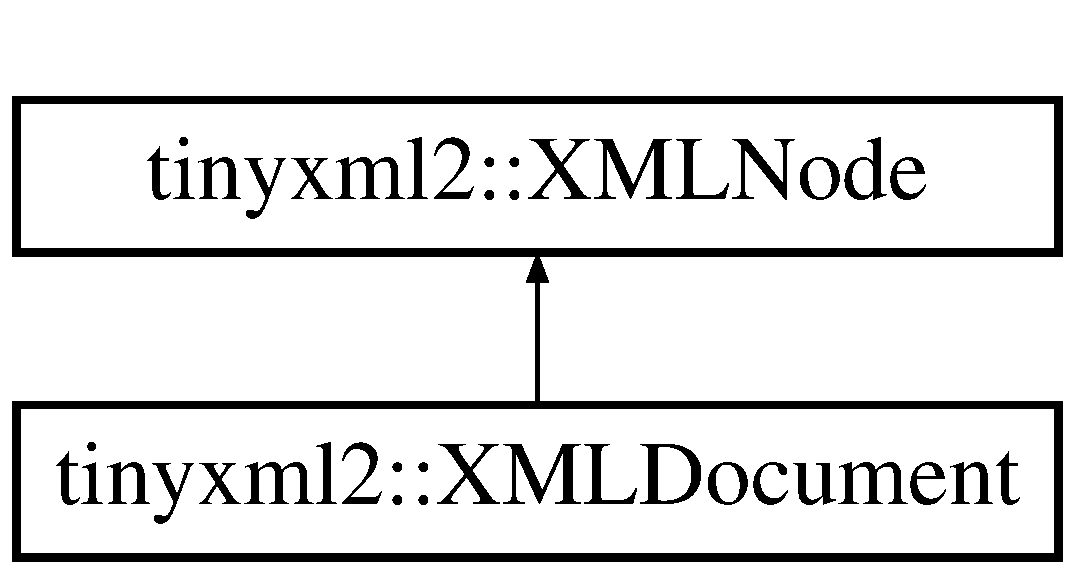
\includegraphics[height=2.000000cm]{classtinyxml2_1_1_x_m_l_document}
\end{center}
\end{figure}
\subsection*{Public Member Functions}
\begin{DoxyCompactItemize}
\item 
\hyperlink{classtinyxml2_1_1_x_m_l_document_af1574f76ebb619f25ef3f09eb2ba5188}{X\+M\+L\+Document} (bool process\+Entities=true, \hyperlink{namespacetinyxml2_a7f91d00f77360f850fd5da0861e27dd5}{Whitespace}=\hyperlink{namespacetinyxml2_a7f91d00f77360f850fd5da0861e27dd5a751769aa625fe5fe5286e9779edec56a}{P\+R\+E\+S\+E\+R\+V\+E\+\_\+\+W\+H\+I\+T\+E\+S\+P\+A\+CE})
\begin{DoxyCompactList}\small\item\em constructor \end{DoxyCompactList}\item 
\hyperlink{classtinyxml2_1_1_x_m_l_document_af37c47d8e2ba4b2fc81b21a77a32579b}{$\sim$\+X\+M\+L\+Document} ()
\item 
virtual \hyperlink{classtinyxml2_1_1_x_m_l_document}{X\+M\+L\+Document} $\ast$ \hyperlink{classtinyxml2_1_1_x_m_l_document_a3e185f880882bd978367bb55937735ec}{To\+Document} ()
\begin{DoxyCompactList}\small\item\em Safely cast to a Document, or null. \end{DoxyCompactList}\item 
virtual const \hyperlink{classtinyxml2_1_1_x_m_l_document}{X\+M\+L\+Document} $\ast$ \hyperlink{classtinyxml2_1_1_x_m_l_document_a747ab173887d969fe313b4617f968e99}{To\+Document} () const
\item 
\hyperlink{namespacetinyxml2_a1fbf88509c3ac88c09117b1947414e08}{X\+M\+L\+Error} \hyperlink{classtinyxml2_1_1_x_m_l_document_a1819bd34f540a7304c105a6232d25a1f}{Parse} (const char $\ast$xml, size\+\_\+t n\+Bytes=(size\+\_\+t)(-\/1))
\item 
\hyperlink{namespacetinyxml2_a1fbf88509c3ac88c09117b1947414e08}{X\+M\+L\+Error} \hyperlink{classtinyxml2_1_1_x_m_l_document_a2ebd4647a8af5fc6831b294ac26a150a}{Load\+File} (const char $\ast$filename)
\item 
\hyperlink{namespacetinyxml2_a1fbf88509c3ac88c09117b1947414e08}{X\+M\+L\+Error} \hyperlink{classtinyxml2_1_1_x_m_l_document_a5f1d330fad44c52f3d265338dd2a6dc2}{Load\+File} (F\+I\+LE $\ast$)
\item 
\hyperlink{namespacetinyxml2_a1fbf88509c3ac88c09117b1947414e08}{X\+M\+L\+Error} \hyperlink{classtinyxml2_1_1_x_m_l_document_a73ac416b4a2aa0952e841220eb3da18f}{Save\+File} (const char $\ast$filename, bool compact=false)
\item 
\hyperlink{namespacetinyxml2_a1fbf88509c3ac88c09117b1947414e08}{X\+M\+L\+Error} \hyperlink{classtinyxml2_1_1_x_m_l_document_a8b95779479a0035acc67b3a61dfe1b74}{Save\+File} (F\+I\+LE $\ast$fp, bool compact=false)
\item 
bool \hyperlink{classtinyxml2_1_1_x_m_l_document_a53e6c035b1b539563fef8c817fb30469}{Process\+Entities} () const
\item 
\hyperlink{namespacetinyxml2_a7f91d00f77360f850fd5da0861e27dd5}{Whitespace} \hyperlink{classtinyxml2_1_1_x_m_l_document_a810ce508e6e0365497c2a9deb83c9ca7}{Whitespace\+Mode} () const
\item 
bool \hyperlink{classtinyxml2_1_1_x_m_l_document_a33fc5d159db873a179fa26338adb05bd}{Has\+B\+OM} () const
\item 
void \hyperlink{classtinyxml2_1_1_x_m_l_document_a14419b698f7c4b140df4e80f3f0c93b0}{Set\+B\+OM} (bool use\+B\+OM)
\item 
\hyperlink{classtinyxml2_1_1_x_m_l_element}{X\+M\+L\+Element} $\ast$ \hyperlink{classtinyxml2_1_1_x_m_l_document_ad2b70320d3c2a071c2f36928edff3e1c}{Root\+Element} ()
\item 
const \hyperlink{classtinyxml2_1_1_x_m_l_element}{X\+M\+L\+Element} $\ast$ \hyperlink{classtinyxml2_1_1_x_m_l_document_a2be8ef9d6346bdef34311f91529afae4}{Root\+Element} () const
\item 
void \hyperlink{classtinyxml2_1_1_x_m_l_document_a867cf5fa3e3ff6ae4847a8b7ee8ec083}{Print} (\hyperlink{classtinyxml2_1_1_x_m_l_printer}{X\+M\+L\+Printer} $\ast$streamer=0) const
\item 
virtual bool \hyperlink{classtinyxml2_1_1_x_m_l_document_ab7be651917a35ab1ff0e4e6d4e565cdf}{Accept} (\hyperlink{classtinyxml2_1_1_x_m_l_visitor}{X\+M\+L\+Visitor} $\ast$visitor) const
\item 
\hyperlink{classtinyxml2_1_1_x_m_l_element}{X\+M\+L\+Element} $\ast$ \hyperlink{classtinyxml2_1_1_x_m_l_document_a3c335a700a43d7c363a393142a23f234}{New\+Element} (const char $\ast$name)
\item 
\hyperlink{classtinyxml2_1_1_x_m_l_comment}{X\+M\+L\+Comment} $\ast$ \hyperlink{classtinyxml2_1_1_x_m_l_document_a386df0befd06aadb5e0cd21381aa955a}{New\+Comment} (const char $\ast$comment)
\item 
\hyperlink{classtinyxml2_1_1_x_m_l_text}{X\+M\+L\+Text} $\ast$ \hyperlink{classtinyxml2_1_1_x_m_l_document_acece5de77a0819f2341b08c1e1ed9987}{New\+Text} (const char $\ast$text)
\item 
\hyperlink{classtinyxml2_1_1_x_m_l_declaration}{X\+M\+L\+Declaration} $\ast$ \hyperlink{classtinyxml2_1_1_x_m_l_document_ae519030c0262fa2daff8993681990e16}{New\+Declaration} (const char $\ast$text=0)
\item 
\hyperlink{classtinyxml2_1_1_x_m_l_unknown}{X\+M\+L\+Unknown} $\ast$ \hyperlink{classtinyxml2_1_1_x_m_l_document_a4954f502c5fd7f49de54c3c0c99bb73d}{New\+Unknown} (const char $\ast$text)
\item 
void \hyperlink{classtinyxml2_1_1_x_m_l_document_ac1d6e2c7fcc1a660624ac4f68e96380d}{Delete\+Node} (\hyperlink{classtinyxml2_1_1_x_m_l_node}{X\+M\+L\+Node} $\ast$node)
\item 
void \hyperlink{classtinyxml2_1_1_x_m_l_document_ab6a90fefdba2b3bb275fc06b72c7c2e6}{Set\+Error} (\hyperlink{namespacetinyxml2_a1fbf88509c3ac88c09117b1947414e08}{X\+M\+L\+Error} error, const char $\ast$str1, const char $\ast$str2, int line\+Num)
\item 
void \hyperlink{classtinyxml2_1_1_x_m_l_document_a4085d9c52f1d93214311459d6d1fcf17}{Clear\+Error} ()
\item 
bool \hyperlink{classtinyxml2_1_1_x_m_l_document_a34e6318e182e40e3cc4f4ba5d59ed9ed}{Error} () const
\begin{DoxyCompactList}\small\item\em Return true if there was an error parsing the document. \end{DoxyCompactList}\item 
\hyperlink{namespacetinyxml2_a1fbf88509c3ac88c09117b1947414e08}{X\+M\+L\+Error} \hyperlink{classtinyxml2_1_1_x_m_l_document_afa3ed33b3107f920ec2b301f805ac17d}{Error\+ID} () const
\begin{DoxyCompactList}\small\item\em Return the error\+ID. \end{DoxyCompactList}\item 
const char $\ast$ \hyperlink{classtinyxml2_1_1_x_m_l_document_a1a5f2b63427caffd4cde15781d9d11f9}{Error\+Name} () const
\item 
const char $\ast$ \hyperlink{classtinyxml2_1_1_x_m_l_document_a229494e30e5473237f3fa547eee4c43f}{Get\+Error\+Str1} () const
\begin{DoxyCompactList}\small\item\em Return a possibly helpful diagnostic location or string. \end{DoxyCompactList}\item 
const char $\ast$ \hyperlink{classtinyxml2_1_1_x_m_l_document_a2d952f49c761bffd2903250680a8716b}{Get\+Error\+Str2} () const
\begin{DoxyCompactList}\small\item\em Return a possibly helpful secondary diagnostic location or string. \end{DoxyCompactList}\item 
int \hyperlink{classtinyxml2_1_1_x_m_l_document_ad82d07e43e096e834dbdfd06312398c1}{Get\+Error\+Line\+Num} () const
\begin{DoxyCompactList}\small\item\em Return the line where the error occured, or zero if unknown. \end{DoxyCompactList}\item 
void \hyperlink{classtinyxml2_1_1_x_m_l_document_a1d033945b42e125d933d6231e4571552}{Print\+Error} () const
\begin{DoxyCompactList}\small\item\em If there is an error, print it to stdout. \end{DoxyCompactList}\item 
void \hyperlink{classtinyxml2_1_1_x_m_l_document_a65656b0b2cbc822708eb351504178aaf}{Clear} ()
\begin{DoxyCompactList}\small\item\em Clear the document, resetting it to the initial state. \end{DoxyCompactList}\item 
char $\ast$ \hyperlink{classtinyxml2_1_1_x_m_l_document_a25827d1bec509ad566a107e5853ed040}{Identify} (char $\ast$p, \hyperlink{classtinyxml2_1_1_x_m_l_node}{X\+M\+L\+Node} $\ast$$\ast$node)
\item 
virtual \hyperlink{classtinyxml2_1_1_x_m_l_node}{X\+M\+L\+Node} $\ast$ \hyperlink{classtinyxml2_1_1_x_m_l_document_aa37cc1709d7e1e988bc17dcfb24a69b8}{Shallow\+Clone} (\hyperlink{classtinyxml2_1_1_x_m_l_document}{X\+M\+L\+Document} $\ast$) const
\item 
virtual bool \hyperlink{classtinyxml2_1_1_x_m_l_document_a6fe5ef18699091844fcf64b56ffa5bf9}{Shallow\+Equal} (const \hyperlink{classtinyxml2_1_1_x_m_l_node}{X\+M\+L\+Node} $\ast$) const
\end{DoxyCompactItemize}
\subsection*{Static Public Member Functions}
\begin{DoxyCompactItemize}
\item 
static const char $\ast$ \hyperlink{classtinyxml2_1_1_x_m_l_document_a639f7c295c38dc5a4aafeb2fff93da03}{Error\+I\+D\+To\+Name} (\hyperlink{namespacetinyxml2_a1fbf88509c3ac88c09117b1947414e08}{X\+M\+L\+Error} error\+ID)
\end{DoxyCompactItemize}
\subsection*{Friends}
\begin{DoxyCompactItemize}
\item 
class \hyperlink{classtinyxml2_1_1_x_m_l_document_ac2fba9b6e452829dd892f7392c24e0eb}{X\+M\+L\+Element}
\end{DoxyCompactItemize}
\subsection*{Additional Inherited Members}


\subsection{Detailed Description}
A Document binds together all the functionality. It can be saved, loaded, and printed to the screen. All Nodes are connected and allocated to a Document. If the Document is deleted, all its Nodes are also deleted. 

\subsection{Constructor \& Destructor Documentation}
\mbox{\Hypertarget{classtinyxml2_1_1_x_m_l_document_af1574f76ebb619f25ef3f09eb2ba5188}\label{classtinyxml2_1_1_x_m_l_document_af1574f76ebb619f25ef3f09eb2ba5188}} 
\index{tinyxml2\+::\+X\+M\+L\+Document@{tinyxml2\+::\+X\+M\+L\+Document}!X\+M\+L\+Document@{X\+M\+L\+Document}}
\index{X\+M\+L\+Document@{X\+M\+L\+Document}!tinyxml2\+::\+X\+M\+L\+Document@{tinyxml2\+::\+X\+M\+L\+Document}}
\subsubsection{\texorpdfstring{X\+M\+L\+Document()}{XMLDocument()}}
{\footnotesize\ttfamily tinyxml2\+::\+X\+M\+L\+Document\+::\+X\+M\+L\+Document (\begin{DoxyParamCaption}\item[{bool}]{process\+Entities = {\ttfamily true},  }\item[{\hyperlink{namespacetinyxml2_a7f91d00f77360f850fd5da0861e27dd5}{Whitespace}}]{whitespace = {\ttfamily \hyperlink{namespacetinyxml2_a7f91d00f77360f850fd5da0861e27dd5a751769aa625fe5fe5286e9779edec56a}{P\+R\+E\+S\+E\+R\+V\+E\+\_\+\+W\+H\+I\+T\+E\+S\+P\+A\+CE}} }\end{DoxyParamCaption})}



constructor 

\mbox{\Hypertarget{classtinyxml2_1_1_x_m_l_document_af37c47d8e2ba4b2fc81b21a77a32579b}\label{classtinyxml2_1_1_x_m_l_document_af37c47d8e2ba4b2fc81b21a77a32579b}} 
\index{tinyxml2\+::\+X\+M\+L\+Document@{tinyxml2\+::\+X\+M\+L\+Document}!````~X\+M\+L\+Document@{$\sim$\+X\+M\+L\+Document}}
\index{````~X\+M\+L\+Document@{$\sim$\+X\+M\+L\+Document}!tinyxml2\+::\+X\+M\+L\+Document@{tinyxml2\+::\+X\+M\+L\+Document}}
\subsubsection{\texorpdfstring{$\sim$\+X\+M\+L\+Document()}{~XMLDocument()}}
{\footnotesize\ttfamily tinyxml2\+::\+X\+M\+L\+Document\+::$\sim$\+X\+M\+L\+Document (\begin{DoxyParamCaption}{ }\end{DoxyParamCaption})}



\subsection{Member Function Documentation}
\mbox{\Hypertarget{classtinyxml2_1_1_x_m_l_document_ab7be651917a35ab1ff0e4e6d4e565cdf}\label{classtinyxml2_1_1_x_m_l_document_ab7be651917a35ab1ff0e4e6d4e565cdf}} 
\index{tinyxml2\+::\+X\+M\+L\+Document@{tinyxml2\+::\+X\+M\+L\+Document}!Accept@{Accept}}
\index{Accept@{Accept}!tinyxml2\+::\+X\+M\+L\+Document@{tinyxml2\+::\+X\+M\+L\+Document}}
\subsubsection{\texorpdfstring{Accept()}{Accept()}}
{\footnotesize\ttfamily bool tinyxml2\+::\+X\+M\+L\+Document\+::\+Accept (\begin{DoxyParamCaption}\item[{\hyperlink{classtinyxml2_1_1_x_m_l_visitor}{X\+M\+L\+Visitor} $\ast$}]{visitor }\end{DoxyParamCaption}) const\hspace{0.3cm}{\ttfamily [virtual]}}

Accept a hierarchical visit of the nodes in the Tiny\+X\+M\+L-\/2 D\+OM. Every node in the X\+ML tree will be conditionally visited and the host will be called back via the \hyperlink{classtinyxml2_1_1_x_m_l_visitor}{X\+M\+L\+Visitor} interface.

This is essentially a S\+AX interface for Tiny\+X\+M\+L-\/2. (Note however it doesn\textquotesingle{}t re-\/parse the X\+ML for the callbacks, so the performance of Tiny\+X\+M\+L-\/2 is unchanged by using this interface versus any other.)

The interface has been based on ideas from\+:


\begin{DoxyItemize}
\item \href{http://www.saxproject.org/}{\tt http\+://www.\+saxproject.\+org/}
\item \href{http://c2.com/cgi/wiki?HierarchicalVisitorPattern}{\tt http\+://c2.\+com/cgi/wiki?\+Hierarchical\+Visitor\+Pattern}
\end{DoxyItemize}

Which are both good references for \char`\"{}visiting\char`\"{}.

An example of using \hyperlink{classtinyxml2_1_1_x_m_l_document_ab7be651917a35ab1ff0e4e6d4e565cdf}{Accept()}\+: \begin{DoxyVerb}XMLPrinter printer;
tinyxmlDoc.Accept( &printer );
const char* xmlcstr = printer.CStr();
\end{DoxyVerb}
 

Implements \hyperlink{classtinyxml2_1_1_x_m_l_node_a81e66df0a44c67a7af17f3b77a152785}{tinyxml2\+::\+X\+M\+L\+Node}.

\mbox{\Hypertarget{classtinyxml2_1_1_x_m_l_document_a65656b0b2cbc822708eb351504178aaf}\label{classtinyxml2_1_1_x_m_l_document_a65656b0b2cbc822708eb351504178aaf}} 
\index{tinyxml2\+::\+X\+M\+L\+Document@{tinyxml2\+::\+X\+M\+L\+Document}!Clear@{Clear}}
\index{Clear@{Clear}!tinyxml2\+::\+X\+M\+L\+Document@{tinyxml2\+::\+X\+M\+L\+Document}}
\subsubsection{\texorpdfstring{Clear()}{Clear()}}
{\footnotesize\ttfamily void tinyxml2\+::\+X\+M\+L\+Document\+::\+Clear (\begin{DoxyParamCaption}{ }\end{DoxyParamCaption})}



Clear the document, resetting it to the initial state. 

\mbox{\Hypertarget{classtinyxml2_1_1_x_m_l_document_a4085d9c52f1d93214311459d6d1fcf17}\label{classtinyxml2_1_1_x_m_l_document_a4085d9c52f1d93214311459d6d1fcf17}} 
\index{tinyxml2\+::\+X\+M\+L\+Document@{tinyxml2\+::\+X\+M\+L\+Document}!Clear\+Error@{Clear\+Error}}
\index{Clear\+Error@{Clear\+Error}!tinyxml2\+::\+X\+M\+L\+Document@{tinyxml2\+::\+X\+M\+L\+Document}}
\subsubsection{\texorpdfstring{Clear\+Error()}{ClearError()}}
{\footnotesize\ttfamily void tinyxml2\+::\+X\+M\+L\+Document\+::\+Clear\+Error (\begin{DoxyParamCaption}{ }\end{DoxyParamCaption})\hspace{0.3cm}{\ttfamily [inline]}}

\mbox{\Hypertarget{classtinyxml2_1_1_x_m_l_document_ac1d6e2c7fcc1a660624ac4f68e96380d}\label{classtinyxml2_1_1_x_m_l_document_ac1d6e2c7fcc1a660624ac4f68e96380d}} 
\index{tinyxml2\+::\+X\+M\+L\+Document@{tinyxml2\+::\+X\+M\+L\+Document}!Delete\+Node@{Delete\+Node}}
\index{Delete\+Node@{Delete\+Node}!tinyxml2\+::\+X\+M\+L\+Document@{tinyxml2\+::\+X\+M\+L\+Document}}
\subsubsection{\texorpdfstring{Delete\+Node()}{DeleteNode()}}
{\footnotesize\ttfamily void tinyxml2\+::\+X\+M\+L\+Document\+::\+Delete\+Node (\begin{DoxyParamCaption}\item[{\hyperlink{classtinyxml2_1_1_x_m_l_node}{X\+M\+L\+Node} $\ast$}]{node }\end{DoxyParamCaption})}

Delete a node associated with this document. It will be unlinked from the D\+OM. \mbox{\Hypertarget{classtinyxml2_1_1_x_m_l_document_a34e6318e182e40e3cc4f4ba5d59ed9ed}\label{classtinyxml2_1_1_x_m_l_document_a34e6318e182e40e3cc4f4ba5d59ed9ed}} 
\index{tinyxml2\+::\+X\+M\+L\+Document@{tinyxml2\+::\+X\+M\+L\+Document}!Error@{Error}}
\index{Error@{Error}!tinyxml2\+::\+X\+M\+L\+Document@{tinyxml2\+::\+X\+M\+L\+Document}}
\subsubsection{\texorpdfstring{Error()}{Error()}}
{\footnotesize\ttfamily bool tinyxml2\+::\+X\+M\+L\+Document\+::\+Error (\begin{DoxyParamCaption}{ }\end{DoxyParamCaption}) const\hspace{0.3cm}{\ttfamily [inline]}}



Return true if there was an error parsing the document. 

\mbox{\Hypertarget{classtinyxml2_1_1_x_m_l_document_afa3ed33b3107f920ec2b301f805ac17d}\label{classtinyxml2_1_1_x_m_l_document_afa3ed33b3107f920ec2b301f805ac17d}} 
\index{tinyxml2\+::\+X\+M\+L\+Document@{tinyxml2\+::\+X\+M\+L\+Document}!Error\+ID@{Error\+ID}}
\index{Error\+ID@{Error\+ID}!tinyxml2\+::\+X\+M\+L\+Document@{tinyxml2\+::\+X\+M\+L\+Document}}
\subsubsection{\texorpdfstring{Error\+I\+D()}{ErrorID()}}
{\footnotesize\ttfamily \hyperlink{namespacetinyxml2_a1fbf88509c3ac88c09117b1947414e08}{X\+M\+L\+Error} tinyxml2\+::\+X\+M\+L\+Document\+::\+Error\+ID (\begin{DoxyParamCaption}{ }\end{DoxyParamCaption}) const\hspace{0.3cm}{\ttfamily [inline]}}



Return the error\+ID. 

\mbox{\Hypertarget{classtinyxml2_1_1_x_m_l_document_a639f7c295c38dc5a4aafeb2fff93da03}\label{classtinyxml2_1_1_x_m_l_document_a639f7c295c38dc5a4aafeb2fff93da03}} 
\index{tinyxml2\+::\+X\+M\+L\+Document@{tinyxml2\+::\+X\+M\+L\+Document}!Error\+I\+D\+To\+Name@{Error\+I\+D\+To\+Name}}
\index{Error\+I\+D\+To\+Name@{Error\+I\+D\+To\+Name}!tinyxml2\+::\+X\+M\+L\+Document@{tinyxml2\+::\+X\+M\+L\+Document}}
\subsubsection{\texorpdfstring{Error\+I\+D\+To\+Name()}{ErrorIDToName()}}
{\footnotesize\ttfamily const char $\ast$ tinyxml2\+::\+X\+M\+L\+Document\+::\+Error\+I\+D\+To\+Name (\begin{DoxyParamCaption}\item[{\hyperlink{namespacetinyxml2_a1fbf88509c3ac88c09117b1947414e08}{X\+M\+L\+Error}}]{error\+ID }\end{DoxyParamCaption})\hspace{0.3cm}{\ttfamily [static]}}

\mbox{\Hypertarget{classtinyxml2_1_1_x_m_l_document_a1a5f2b63427caffd4cde15781d9d11f9}\label{classtinyxml2_1_1_x_m_l_document_a1a5f2b63427caffd4cde15781d9d11f9}} 
\index{tinyxml2\+::\+X\+M\+L\+Document@{tinyxml2\+::\+X\+M\+L\+Document}!Error\+Name@{Error\+Name}}
\index{Error\+Name@{Error\+Name}!tinyxml2\+::\+X\+M\+L\+Document@{tinyxml2\+::\+X\+M\+L\+Document}}
\subsubsection{\texorpdfstring{Error\+Name()}{ErrorName()}}
{\footnotesize\ttfamily const char $\ast$ tinyxml2\+::\+X\+M\+L\+Document\+::\+Error\+Name (\begin{DoxyParamCaption}{ }\end{DoxyParamCaption}) const}

\mbox{\Hypertarget{classtinyxml2_1_1_x_m_l_document_ad82d07e43e096e834dbdfd06312398c1}\label{classtinyxml2_1_1_x_m_l_document_ad82d07e43e096e834dbdfd06312398c1}} 
\index{tinyxml2\+::\+X\+M\+L\+Document@{tinyxml2\+::\+X\+M\+L\+Document}!Get\+Error\+Line\+Num@{Get\+Error\+Line\+Num}}
\index{Get\+Error\+Line\+Num@{Get\+Error\+Line\+Num}!tinyxml2\+::\+X\+M\+L\+Document@{tinyxml2\+::\+X\+M\+L\+Document}}
\subsubsection{\texorpdfstring{Get\+Error\+Line\+Num()}{GetErrorLineNum()}}
{\footnotesize\ttfamily int tinyxml2\+::\+X\+M\+L\+Document\+::\+Get\+Error\+Line\+Num (\begin{DoxyParamCaption}{ }\end{DoxyParamCaption}) const\hspace{0.3cm}{\ttfamily [inline]}}



Return the line where the error occured, or zero if unknown. 

\mbox{\Hypertarget{classtinyxml2_1_1_x_m_l_document_a229494e30e5473237f3fa547eee4c43f}\label{classtinyxml2_1_1_x_m_l_document_a229494e30e5473237f3fa547eee4c43f}} 
\index{tinyxml2\+::\+X\+M\+L\+Document@{tinyxml2\+::\+X\+M\+L\+Document}!Get\+Error\+Str1@{Get\+Error\+Str1}}
\index{Get\+Error\+Str1@{Get\+Error\+Str1}!tinyxml2\+::\+X\+M\+L\+Document@{tinyxml2\+::\+X\+M\+L\+Document}}
\subsubsection{\texorpdfstring{Get\+Error\+Str1()}{GetErrorStr1()}}
{\footnotesize\ttfamily const char$\ast$ tinyxml2\+::\+X\+M\+L\+Document\+::\+Get\+Error\+Str1 (\begin{DoxyParamCaption}{ }\end{DoxyParamCaption}) const\hspace{0.3cm}{\ttfamily [inline]}}



Return a possibly helpful diagnostic location or string. 

\mbox{\Hypertarget{classtinyxml2_1_1_x_m_l_document_a2d952f49c761bffd2903250680a8716b}\label{classtinyxml2_1_1_x_m_l_document_a2d952f49c761bffd2903250680a8716b}} 
\index{tinyxml2\+::\+X\+M\+L\+Document@{tinyxml2\+::\+X\+M\+L\+Document}!Get\+Error\+Str2@{Get\+Error\+Str2}}
\index{Get\+Error\+Str2@{Get\+Error\+Str2}!tinyxml2\+::\+X\+M\+L\+Document@{tinyxml2\+::\+X\+M\+L\+Document}}
\subsubsection{\texorpdfstring{Get\+Error\+Str2()}{GetErrorStr2()}}
{\footnotesize\ttfamily const char$\ast$ tinyxml2\+::\+X\+M\+L\+Document\+::\+Get\+Error\+Str2 (\begin{DoxyParamCaption}{ }\end{DoxyParamCaption}) const\hspace{0.3cm}{\ttfamily [inline]}}



Return a possibly helpful secondary diagnostic location or string. 

\mbox{\Hypertarget{classtinyxml2_1_1_x_m_l_document_a33fc5d159db873a179fa26338adb05bd}\label{classtinyxml2_1_1_x_m_l_document_a33fc5d159db873a179fa26338adb05bd}} 
\index{tinyxml2\+::\+X\+M\+L\+Document@{tinyxml2\+::\+X\+M\+L\+Document}!Has\+B\+OM@{Has\+B\+OM}}
\index{Has\+B\+OM@{Has\+B\+OM}!tinyxml2\+::\+X\+M\+L\+Document@{tinyxml2\+::\+X\+M\+L\+Document}}
\subsubsection{\texorpdfstring{Has\+B\+O\+M()}{HasBOM()}}
{\footnotesize\ttfamily bool tinyxml2\+::\+X\+M\+L\+Document\+::\+Has\+B\+OM (\begin{DoxyParamCaption}{ }\end{DoxyParamCaption}) const\hspace{0.3cm}{\ttfamily [inline]}}

Returns true if this document has a leading Byte Order Mark of U\+T\+F8. \mbox{\Hypertarget{classtinyxml2_1_1_x_m_l_document_a25827d1bec509ad566a107e5853ed040}\label{classtinyxml2_1_1_x_m_l_document_a25827d1bec509ad566a107e5853ed040}} 
\index{tinyxml2\+::\+X\+M\+L\+Document@{tinyxml2\+::\+X\+M\+L\+Document}!Identify@{Identify}}
\index{Identify@{Identify}!tinyxml2\+::\+X\+M\+L\+Document@{tinyxml2\+::\+X\+M\+L\+Document}}
\subsubsection{\texorpdfstring{Identify()}{Identify()}}
{\footnotesize\ttfamily char $\ast$ tinyxml2\+::\+X\+M\+L\+Document\+::\+Identify (\begin{DoxyParamCaption}\item[{char $\ast$}]{p,  }\item[{\hyperlink{classtinyxml2_1_1_x_m_l_node}{X\+M\+L\+Node} $\ast$$\ast$}]{node }\end{DoxyParamCaption})}

\mbox{\Hypertarget{classtinyxml2_1_1_x_m_l_document_a2ebd4647a8af5fc6831b294ac26a150a}\label{classtinyxml2_1_1_x_m_l_document_a2ebd4647a8af5fc6831b294ac26a150a}} 
\index{tinyxml2\+::\+X\+M\+L\+Document@{tinyxml2\+::\+X\+M\+L\+Document}!Load\+File@{Load\+File}}
\index{Load\+File@{Load\+File}!tinyxml2\+::\+X\+M\+L\+Document@{tinyxml2\+::\+X\+M\+L\+Document}}
\subsubsection{\texorpdfstring{Load\+File()}{LoadFile()}\hspace{0.1cm}{\footnotesize\ttfamily [1/2]}}
{\footnotesize\ttfamily \hyperlink{namespacetinyxml2_a1fbf88509c3ac88c09117b1947414e08}{X\+M\+L\+Error} tinyxml2\+::\+X\+M\+L\+Document\+::\+Load\+File (\begin{DoxyParamCaption}\item[{const char $\ast$}]{filename }\end{DoxyParamCaption})}

Load an X\+ML file from disk. Returns X\+M\+L\+\_\+\+S\+U\+C\+C\+E\+SS (0) on success, or an error\+ID. \mbox{\Hypertarget{classtinyxml2_1_1_x_m_l_document_a5f1d330fad44c52f3d265338dd2a6dc2}\label{classtinyxml2_1_1_x_m_l_document_a5f1d330fad44c52f3d265338dd2a6dc2}} 
\index{tinyxml2\+::\+X\+M\+L\+Document@{tinyxml2\+::\+X\+M\+L\+Document}!Load\+File@{Load\+File}}
\index{Load\+File@{Load\+File}!tinyxml2\+::\+X\+M\+L\+Document@{tinyxml2\+::\+X\+M\+L\+Document}}
\subsubsection{\texorpdfstring{Load\+File()}{LoadFile()}\hspace{0.1cm}{\footnotesize\ttfamily [2/2]}}
{\footnotesize\ttfamily \hyperlink{namespacetinyxml2_a1fbf88509c3ac88c09117b1947414e08}{X\+M\+L\+Error} tinyxml2\+::\+X\+M\+L\+Document\+::\+Load\+File (\begin{DoxyParamCaption}\item[{F\+I\+LE $\ast$}]{fp }\end{DoxyParamCaption})}

Load an X\+ML file from disk. You are responsible for providing and closing the F\+I\+L\+E$\ast$.

N\+O\+TE\+: The file should be opened as binary (\char`\"{}rb\char`\"{}) not text in order for Tiny\+X\+M\+L-\/2 to correctly do newline normalization.

Returns X\+M\+L\+\_\+\+S\+U\+C\+C\+E\+SS (0) on success, or an error\+ID. \mbox{\Hypertarget{classtinyxml2_1_1_x_m_l_document_a386df0befd06aadb5e0cd21381aa955a}\label{classtinyxml2_1_1_x_m_l_document_a386df0befd06aadb5e0cd21381aa955a}} 
\index{tinyxml2\+::\+X\+M\+L\+Document@{tinyxml2\+::\+X\+M\+L\+Document}!New\+Comment@{New\+Comment}}
\index{New\+Comment@{New\+Comment}!tinyxml2\+::\+X\+M\+L\+Document@{tinyxml2\+::\+X\+M\+L\+Document}}
\subsubsection{\texorpdfstring{New\+Comment()}{NewComment()}}
{\footnotesize\ttfamily \hyperlink{classtinyxml2_1_1_x_m_l_comment}{X\+M\+L\+Comment} $\ast$ tinyxml2\+::\+X\+M\+L\+Document\+::\+New\+Comment (\begin{DoxyParamCaption}\item[{const char $\ast$}]{comment }\end{DoxyParamCaption})}

Create a new Comment associated with this Document. The memory for the Comment is managed by the Document. \mbox{\Hypertarget{classtinyxml2_1_1_x_m_l_document_ae519030c0262fa2daff8993681990e16}\label{classtinyxml2_1_1_x_m_l_document_ae519030c0262fa2daff8993681990e16}} 
\index{tinyxml2\+::\+X\+M\+L\+Document@{tinyxml2\+::\+X\+M\+L\+Document}!New\+Declaration@{New\+Declaration}}
\index{New\+Declaration@{New\+Declaration}!tinyxml2\+::\+X\+M\+L\+Document@{tinyxml2\+::\+X\+M\+L\+Document}}
\subsubsection{\texorpdfstring{New\+Declaration()}{NewDeclaration()}}
{\footnotesize\ttfamily \hyperlink{classtinyxml2_1_1_x_m_l_declaration}{X\+M\+L\+Declaration} $\ast$ tinyxml2\+::\+X\+M\+L\+Document\+::\+New\+Declaration (\begin{DoxyParamCaption}\item[{const char $\ast$}]{text = {\ttfamily 0} }\end{DoxyParamCaption})}

Create a new Declaration associated with this Document. The memory for the object is managed by the Document.

If the \textquotesingle{}text\textquotesingle{} param is null, the standard declaration is used.\+: \begin{DoxyVerb}<?xml version="1.0" encoding="UTF-8"?>
\end{DoxyVerb}
 \mbox{\Hypertarget{classtinyxml2_1_1_x_m_l_document_a3c335a700a43d7c363a393142a23f234}\label{classtinyxml2_1_1_x_m_l_document_a3c335a700a43d7c363a393142a23f234}} 
\index{tinyxml2\+::\+X\+M\+L\+Document@{tinyxml2\+::\+X\+M\+L\+Document}!New\+Element@{New\+Element}}
\index{New\+Element@{New\+Element}!tinyxml2\+::\+X\+M\+L\+Document@{tinyxml2\+::\+X\+M\+L\+Document}}
\subsubsection{\texorpdfstring{New\+Element()}{NewElement()}}
{\footnotesize\ttfamily \hyperlink{classtinyxml2_1_1_x_m_l_element}{X\+M\+L\+Element} $\ast$ tinyxml2\+::\+X\+M\+L\+Document\+::\+New\+Element (\begin{DoxyParamCaption}\item[{const char $\ast$}]{name }\end{DoxyParamCaption})}

Create a new Element associated with this Document. The memory for the Element is managed by the Document. \mbox{\Hypertarget{classtinyxml2_1_1_x_m_l_document_acece5de77a0819f2341b08c1e1ed9987}\label{classtinyxml2_1_1_x_m_l_document_acece5de77a0819f2341b08c1e1ed9987}} 
\index{tinyxml2\+::\+X\+M\+L\+Document@{tinyxml2\+::\+X\+M\+L\+Document}!New\+Text@{New\+Text}}
\index{New\+Text@{New\+Text}!tinyxml2\+::\+X\+M\+L\+Document@{tinyxml2\+::\+X\+M\+L\+Document}}
\subsubsection{\texorpdfstring{New\+Text()}{NewText()}}
{\footnotesize\ttfamily \hyperlink{classtinyxml2_1_1_x_m_l_text}{X\+M\+L\+Text} $\ast$ tinyxml2\+::\+X\+M\+L\+Document\+::\+New\+Text (\begin{DoxyParamCaption}\item[{const char $\ast$}]{text }\end{DoxyParamCaption})}

Create a new Text associated with this Document. The memory for the Text is managed by the Document. \mbox{\Hypertarget{classtinyxml2_1_1_x_m_l_document_a4954f502c5fd7f49de54c3c0c99bb73d}\label{classtinyxml2_1_1_x_m_l_document_a4954f502c5fd7f49de54c3c0c99bb73d}} 
\index{tinyxml2\+::\+X\+M\+L\+Document@{tinyxml2\+::\+X\+M\+L\+Document}!New\+Unknown@{New\+Unknown}}
\index{New\+Unknown@{New\+Unknown}!tinyxml2\+::\+X\+M\+L\+Document@{tinyxml2\+::\+X\+M\+L\+Document}}
\subsubsection{\texorpdfstring{New\+Unknown()}{NewUnknown()}}
{\footnotesize\ttfamily \hyperlink{classtinyxml2_1_1_x_m_l_unknown}{X\+M\+L\+Unknown} $\ast$ tinyxml2\+::\+X\+M\+L\+Document\+::\+New\+Unknown (\begin{DoxyParamCaption}\item[{const char $\ast$}]{text }\end{DoxyParamCaption})}

Create a new Unknown associated with this Document. The memory for the object is managed by the Document. \mbox{\Hypertarget{classtinyxml2_1_1_x_m_l_document_a1819bd34f540a7304c105a6232d25a1f}\label{classtinyxml2_1_1_x_m_l_document_a1819bd34f540a7304c105a6232d25a1f}} 
\index{tinyxml2\+::\+X\+M\+L\+Document@{tinyxml2\+::\+X\+M\+L\+Document}!Parse@{Parse}}
\index{Parse@{Parse}!tinyxml2\+::\+X\+M\+L\+Document@{tinyxml2\+::\+X\+M\+L\+Document}}
\subsubsection{\texorpdfstring{Parse()}{Parse()}}
{\footnotesize\ttfamily \hyperlink{namespacetinyxml2_a1fbf88509c3ac88c09117b1947414e08}{X\+M\+L\+Error} tinyxml2\+::\+X\+M\+L\+Document\+::\+Parse (\begin{DoxyParamCaption}\item[{const char $\ast$}]{xml,  }\item[{size\+\_\+t}]{n\+Bytes = {\ttfamily (size\+\_\+t)(-\/1)} }\end{DoxyParamCaption})}

Parse an X\+ML file from a character string. Returns X\+M\+L\+\_\+\+S\+U\+C\+C\+E\+SS (0) on success, or an error\+ID.

You may optionally pass in the \textquotesingle{}n\+Bytes\textquotesingle{}, which is the number of bytes which will be parsed. If not specified, Tiny\+X\+M\+L-\/2 will assume \textquotesingle{}xml\textquotesingle{} points to a null terminated string. \mbox{\Hypertarget{classtinyxml2_1_1_x_m_l_document_a867cf5fa3e3ff6ae4847a8b7ee8ec083}\label{classtinyxml2_1_1_x_m_l_document_a867cf5fa3e3ff6ae4847a8b7ee8ec083}} 
\index{tinyxml2\+::\+X\+M\+L\+Document@{tinyxml2\+::\+X\+M\+L\+Document}!Print@{Print}}
\index{Print@{Print}!tinyxml2\+::\+X\+M\+L\+Document@{tinyxml2\+::\+X\+M\+L\+Document}}
\subsubsection{\texorpdfstring{Print()}{Print()}}
{\footnotesize\ttfamily void tinyxml2\+::\+X\+M\+L\+Document\+::\+Print (\begin{DoxyParamCaption}\item[{\hyperlink{classtinyxml2_1_1_x_m_l_printer}{X\+M\+L\+Printer} $\ast$}]{streamer = {\ttfamily 0} }\end{DoxyParamCaption}) const}

Print the Document. If the Printer is not provided, it will print to stdout. If you provide Printer, this can print to a file\+: \begin{DoxyVerb}XMLPrinter printer( fp );
doc.Print( &printer );
\end{DoxyVerb}


Or you can use a printer to print to memory\+: \begin{DoxyVerb}XMLPrinter printer;
doc.Print( &printer );
// printer.CStr() has a const char* to the XML
\end{DoxyVerb}
 \mbox{\Hypertarget{classtinyxml2_1_1_x_m_l_document_a1d033945b42e125d933d6231e4571552}\label{classtinyxml2_1_1_x_m_l_document_a1d033945b42e125d933d6231e4571552}} 
\index{tinyxml2\+::\+X\+M\+L\+Document@{tinyxml2\+::\+X\+M\+L\+Document}!Print\+Error@{Print\+Error}}
\index{Print\+Error@{Print\+Error}!tinyxml2\+::\+X\+M\+L\+Document@{tinyxml2\+::\+X\+M\+L\+Document}}
\subsubsection{\texorpdfstring{Print\+Error()}{PrintError()}}
{\footnotesize\ttfamily void tinyxml2\+::\+X\+M\+L\+Document\+::\+Print\+Error (\begin{DoxyParamCaption}{ }\end{DoxyParamCaption}) const}



If there is an error, print it to stdout. 

\mbox{\Hypertarget{classtinyxml2_1_1_x_m_l_document_a53e6c035b1b539563fef8c817fb30469}\label{classtinyxml2_1_1_x_m_l_document_a53e6c035b1b539563fef8c817fb30469}} 
\index{tinyxml2\+::\+X\+M\+L\+Document@{tinyxml2\+::\+X\+M\+L\+Document}!Process\+Entities@{Process\+Entities}}
\index{Process\+Entities@{Process\+Entities}!tinyxml2\+::\+X\+M\+L\+Document@{tinyxml2\+::\+X\+M\+L\+Document}}
\subsubsection{\texorpdfstring{Process\+Entities()}{ProcessEntities()}}
{\footnotesize\ttfamily bool tinyxml2\+::\+X\+M\+L\+Document\+::\+Process\+Entities (\begin{DoxyParamCaption}{ }\end{DoxyParamCaption}) const\hspace{0.3cm}{\ttfamily [inline]}}

\mbox{\Hypertarget{classtinyxml2_1_1_x_m_l_document_ad2b70320d3c2a071c2f36928edff3e1c}\label{classtinyxml2_1_1_x_m_l_document_ad2b70320d3c2a071c2f36928edff3e1c}} 
\index{tinyxml2\+::\+X\+M\+L\+Document@{tinyxml2\+::\+X\+M\+L\+Document}!Root\+Element@{Root\+Element}}
\index{Root\+Element@{Root\+Element}!tinyxml2\+::\+X\+M\+L\+Document@{tinyxml2\+::\+X\+M\+L\+Document}}
\subsubsection{\texorpdfstring{Root\+Element()}{RootElement()}\hspace{0.1cm}{\footnotesize\ttfamily [1/2]}}
{\footnotesize\ttfamily \hyperlink{classtinyxml2_1_1_x_m_l_element}{X\+M\+L\+Element}$\ast$ tinyxml2\+::\+X\+M\+L\+Document\+::\+Root\+Element (\begin{DoxyParamCaption}{ }\end{DoxyParamCaption})\hspace{0.3cm}{\ttfamily [inline]}}

Return the root element of D\+OM. Equivalent to \hyperlink{classtinyxml2_1_1_x_m_l_node_a1bec132dcf085284e0a10755f2cf0d57}{First\+Child\+Element()}. To get the first node, use \hyperlink{classtinyxml2_1_1_x_m_l_node_a2d6c70c475146b48bc93a7fafdeff5e0}{First\+Child()}. \mbox{\Hypertarget{classtinyxml2_1_1_x_m_l_document_a2be8ef9d6346bdef34311f91529afae4}\label{classtinyxml2_1_1_x_m_l_document_a2be8ef9d6346bdef34311f91529afae4}} 
\index{tinyxml2\+::\+X\+M\+L\+Document@{tinyxml2\+::\+X\+M\+L\+Document}!Root\+Element@{Root\+Element}}
\index{Root\+Element@{Root\+Element}!tinyxml2\+::\+X\+M\+L\+Document@{tinyxml2\+::\+X\+M\+L\+Document}}
\subsubsection{\texorpdfstring{Root\+Element()}{RootElement()}\hspace{0.1cm}{\footnotesize\ttfamily [2/2]}}
{\footnotesize\ttfamily const \hyperlink{classtinyxml2_1_1_x_m_l_element}{X\+M\+L\+Element}$\ast$ tinyxml2\+::\+X\+M\+L\+Document\+::\+Root\+Element (\begin{DoxyParamCaption}{ }\end{DoxyParamCaption}) const\hspace{0.3cm}{\ttfamily [inline]}}

\mbox{\Hypertarget{classtinyxml2_1_1_x_m_l_document_a73ac416b4a2aa0952e841220eb3da18f}\label{classtinyxml2_1_1_x_m_l_document_a73ac416b4a2aa0952e841220eb3da18f}} 
\index{tinyxml2\+::\+X\+M\+L\+Document@{tinyxml2\+::\+X\+M\+L\+Document}!Save\+File@{Save\+File}}
\index{Save\+File@{Save\+File}!tinyxml2\+::\+X\+M\+L\+Document@{tinyxml2\+::\+X\+M\+L\+Document}}
\subsubsection{\texorpdfstring{Save\+File()}{SaveFile()}\hspace{0.1cm}{\footnotesize\ttfamily [1/2]}}
{\footnotesize\ttfamily \hyperlink{namespacetinyxml2_a1fbf88509c3ac88c09117b1947414e08}{X\+M\+L\+Error} tinyxml2\+::\+X\+M\+L\+Document\+::\+Save\+File (\begin{DoxyParamCaption}\item[{const char $\ast$}]{filename,  }\item[{bool}]{compact = {\ttfamily false} }\end{DoxyParamCaption})}

Save the X\+ML file to disk. Returns X\+M\+L\+\_\+\+S\+U\+C\+C\+E\+SS (0) on success, or an error\+ID. \mbox{\Hypertarget{classtinyxml2_1_1_x_m_l_document_a8b95779479a0035acc67b3a61dfe1b74}\label{classtinyxml2_1_1_x_m_l_document_a8b95779479a0035acc67b3a61dfe1b74}} 
\index{tinyxml2\+::\+X\+M\+L\+Document@{tinyxml2\+::\+X\+M\+L\+Document}!Save\+File@{Save\+File}}
\index{Save\+File@{Save\+File}!tinyxml2\+::\+X\+M\+L\+Document@{tinyxml2\+::\+X\+M\+L\+Document}}
\subsubsection{\texorpdfstring{Save\+File()}{SaveFile()}\hspace{0.1cm}{\footnotesize\ttfamily [2/2]}}
{\footnotesize\ttfamily \hyperlink{namespacetinyxml2_a1fbf88509c3ac88c09117b1947414e08}{X\+M\+L\+Error} tinyxml2\+::\+X\+M\+L\+Document\+::\+Save\+File (\begin{DoxyParamCaption}\item[{F\+I\+LE $\ast$}]{fp,  }\item[{bool}]{compact = {\ttfamily false} }\end{DoxyParamCaption})}

Save the X\+ML file to disk. You are responsible for providing and closing the F\+I\+L\+E$\ast$.

Returns X\+M\+L\+\_\+\+S\+U\+C\+C\+E\+SS (0) on success, or an error\+ID. \mbox{\Hypertarget{classtinyxml2_1_1_x_m_l_document_a14419b698f7c4b140df4e80f3f0c93b0}\label{classtinyxml2_1_1_x_m_l_document_a14419b698f7c4b140df4e80f3f0c93b0}} 
\index{tinyxml2\+::\+X\+M\+L\+Document@{tinyxml2\+::\+X\+M\+L\+Document}!Set\+B\+OM@{Set\+B\+OM}}
\index{Set\+B\+OM@{Set\+B\+OM}!tinyxml2\+::\+X\+M\+L\+Document@{tinyxml2\+::\+X\+M\+L\+Document}}
\subsubsection{\texorpdfstring{Set\+B\+O\+M()}{SetBOM()}}
{\footnotesize\ttfamily void tinyxml2\+::\+X\+M\+L\+Document\+::\+Set\+B\+OM (\begin{DoxyParamCaption}\item[{bool}]{use\+B\+OM }\end{DoxyParamCaption})\hspace{0.3cm}{\ttfamily [inline]}}

Sets whether to write the B\+OM when writing the file. \mbox{\Hypertarget{classtinyxml2_1_1_x_m_l_document_ab6a90fefdba2b3bb275fc06b72c7c2e6}\label{classtinyxml2_1_1_x_m_l_document_ab6a90fefdba2b3bb275fc06b72c7c2e6}} 
\index{tinyxml2\+::\+X\+M\+L\+Document@{tinyxml2\+::\+X\+M\+L\+Document}!Set\+Error@{Set\+Error}}
\index{Set\+Error@{Set\+Error}!tinyxml2\+::\+X\+M\+L\+Document@{tinyxml2\+::\+X\+M\+L\+Document}}
\subsubsection{\texorpdfstring{Set\+Error()}{SetError()}}
{\footnotesize\ttfamily void tinyxml2\+::\+X\+M\+L\+Document\+::\+Set\+Error (\begin{DoxyParamCaption}\item[{\hyperlink{namespacetinyxml2_a1fbf88509c3ac88c09117b1947414e08}{X\+M\+L\+Error}}]{error,  }\item[{const char $\ast$}]{str1,  }\item[{const char $\ast$}]{str2,  }\item[{int}]{line\+Num }\end{DoxyParamCaption})}

\mbox{\Hypertarget{classtinyxml2_1_1_x_m_l_document_aa37cc1709d7e1e988bc17dcfb24a69b8}\label{classtinyxml2_1_1_x_m_l_document_aa37cc1709d7e1e988bc17dcfb24a69b8}} 
\index{tinyxml2\+::\+X\+M\+L\+Document@{tinyxml2\+::\+X\+M\+L\+Document}!Shallow\+Clone@{Shallow\+Clone}}
\index{Shallow\+Clone@{Shallow\+Clone}!tinyxml2\+::\+X\+M\+L\+Document@{tinyxml2\+::\+X\+M\+L\+Document}}
\subsubsection{\texorpdfstring{Shallow\+Clone()}{ShallowClone()}}
{\footnotesize\ttfamily virtual \hyperlink{classtinyxml2_1_1_x_m_l_node}{X\+M\+L\+Node}$\ast$ tinyxml2\+::\+X\+M\+L\+Document\+::\+Shallow\+Clone (\begin{DoxyParamCaption}\item[{\hyperlink{classtinyxml2_1_1_x_m_l_document}{X\+M\+L\+Document} $\ast$}]{document }\end{DoxyParamCaption}) const\hspace{0.3cm}{\ttfamily [inline]}, {\ttfamily [virtual]}}

Make a copy of this node, but not its children. You may pass in a Document pointer that will be the owner of the new Node. If the \textquotesingle{}document\textquotesingle{} is null, then the node returned will be allocated from the current Document. (this-\/$>$\hyperlink{classtinyxml2_1_1_x_m_l_node_af343d1ef0b45c0020e62d784d7e67a68}{Get\+Document()})

Note\+: if called on a \hyperlink{classtinyxml2_1_1_x_m_l_document}{X\+M\+L\+Document}, this will return null. 

Implements \hyperlink{classtinyxml2_1_1_x_m_l_node_a8402cbd3129d20e9e6024bbcc0531283}{tinyxml2\+::\+X\+M\+L\+Node}.

\mbox{\Hypertarget{classtinyxml2_1_1_x_m_l_document_a6fe5ef18699091844fcf64b56ffa5bf9}\label{classtinyxml2_1_1_x_m_l_document_a6fe5ef18699091844fcf64b56ffa5bf9}} 
\index{tinyxml2\+::\+X\+M\+L\+Document@{tinyxml2\+::\+X\+M\+L\+Document}!Shallow\+Equal@{Shallow\+Equal}}
\index{Shallow\+Equal@{Shallow\+Equal}!tinyxml2\+::\+X\+M\+L\+Document@{tinyxml2\+::\+X\+M\+L\+Document}}
\subsubsection{\texorpdfstring{Shallow\+Equal()}{ShallowEqual()}}
{\footnotesize\ttfamily virtual bool tinyxml2\+::\+X\+M\+L\+Document\+::\+Shallow\+Equal (\begin{DoxyParamCaption}\item[{const \hyperlink{classtinyxml2_1_1_x_m_l_node}{X\+M\+L\+Node} $\ast$}]{compare }\end{DoxyParamCaption}) const\hspace{0.3cm}{\ttfamily [inline]}, {\ttfamily [virtual]}}

Test if 2 nodes are the same, but don\textquotesingle{}t test children. The 2 nodes do not need to be in the same Document.

Note\+: if called on a \hyperlink{classtinyxml2_1_1_x_m_l_document}{X\+M\+L\+Document}, this will return false. 

Implements \hyperlink{classtinyxml2_1_1_x_m_l_node_a7ce18b751c3ea09eac292dca264f9226}{tinyxml2\+::\+X\+M\+L\+Node}.

\mbox{\Hypertarget{classtinyxml2_1_1_x_m_l_document_a3e185f880882bd978367bb55937735ec}\label{classtinyxml2_1_1_x_m_l_document_a3e185f880882bd978367bb55937735ec}} 
\index{tinyxml2\+::\+X\+M\+L\+Document@{tinyxml2\+::\+X\+M\+L\+Document}!To\+Document@{To\+Document}}
\index{To\+Document@{To\+Document}!tinyxml2\+::\+X\+M\+L\+Document@{tinyxml2\+::\+X\+M\+L\+Document}}
\subsubsection{\texorpdfstring{To\+Document()}{ToDocument()}\hspace{0.1cm}{\footnotesize\ttfamily [1/2]}}
{\footnotesize\ttfamily virtual \hyperlink{classtinyxml2_1_1_x_m_l_document}{X\+M\+L\+Document}$\ast$ tinyxml2\+::\+X\+M\+L\+Document\+::\+To\+Document (\begin{DoxyParamCaption}{ }\end{DoxyParamCaption})\hspace{0.3cm}{\ttfamily [inline]}, {\ttfamily [virtual]}}



Safely cast to a Document, or null. 



Reimplemented from \hyperlink{classtinyxml2_1_1_x_m_l_node_a836e2966ed736fc3c94f70e12a2a3357}{tinyxml2\+::\+X\+M\+L\+Node}.

\mbox{\Hypertarget{classtinyxml2_1_1_x_m_l_document_a747ab173887d969fe313b4617f968e99}\label{classtinyxml2_1_1_x_m_l_document_a747ab173887d969fe313b4617f968e99}} 
\index{tinyxml2\+::\+X\+M\+L\+Document@{tinyxml2\+::\+X\+M\+L\+Document}!To\+Document@{To\+Document}}
\index{To\+Document@{To\+Document}!tinyxml2\+::\+X\+M\+L\+Document@{tinyxml2\+::\+X\+M\+L\+Document}}
\subsubsection{\texorpdfstring{To\+Document()}{ToDocument()}\hspace{0.1cm}{\footnotesize\ttfamily [2/2]}}
{\footnotesize\ttfamily virtual const \hyperlink{classtinyxml2_1_1_x_m_l_document}{X\+M\+L\+Document}$\ast$ tinyxml2\+::\+X\+M\+L\+Document\+::\+To\+Document (\begin{DoxyParamCaption}{ }\end{DoxyParamCaption}) const\hspace{0.3cm}{\ttfamily [inline]}, {\ttfamily [virtual]}}



Reimplemented from \hyperlink{classtinyxml2_1_1_x_m_l_node_ae8a5250331a5f12e10843fcb5ef3ef0b}{tinyxml2\+::\+X\+M\+L\+Node}.

\mbox{\Hypertarget{classtinyxml2_1_1_x_m_l_document_a810ce508e6e0365497c2a9deb83c9ca7}\label{classtinyxml2_1_1_x_m_l_document_a810ce508e6e0365497c2a9deb83c9ca7}} 
\index{tinyxml2\+::\+X\+M\+L\+Document@{tinyxml2\+::\+X\+M\+L\+Document}!Whitespace\+Mode@{Whitespace\+Mode}}
\index{Whitespace\+Mode@{Whitespace\+Mode}!tinyxml2\+::\+X\+M\+L\+Document@{tinyxml2\+::\+X\+M\+L\+Document}}
\subsubsection{\texorpdfstring{Whitespace\+Mode()}{WhitespaceMode()}}
{\footnotesize\ttfamily \hyperlink{namespacetinyxml2_a7f91d00f77360f850fd5da0861e27dd5}{Whitespace} tinyxml2\+::\+X\+M\+L\+Document\+::\+Whitespace\+Mode (\begin{DoxyParamCaption}{ }\end{DoxyParamCaption}) const\hspace{0.3cm}{\ttfamily [inline]}}



\subsection{Friends And Related Function Documentation}
\mbox{\Hypertarget{classtinyxml2_1_1_x_m_l_document_ac2fba9b6e452829dd892f7392c24e0eb}\label{classtinyxml2_1_1_x_m_l_document_ac2fba9b6e452829dd892f7392c24e0eb}} 
\index{tinyxml2\+::\+X\+M\+L\+Document@{tinyxml2\+::\+X\+M\+L\+Document}!X\+M\+L\+Element@{X\+M\+L\+Element}}
\index{X\+M\+L\+Element@{X\+M\+L\+Element}!tinyxml2\+::\+X\+M\+L\+Document@{tinyxml2\+::\+X\+M\+L\+Document}}
\subsubsection{\texorpdfstring{X\+M\+L\+Element}{XMLElement}}
{\footnotesize\ttfamily friend class \hyperlink{classtinyxml2_1_1_x_m_l_element}{X\+M\+L\+Element}\hspace{0.3cm}{\ttfamily [friend]}}



The documentation for this class was generated from the following files\+:\begin{DoxyCompactItemize}
\item 
\hyperlink{tinyxml2_8h}{tinyxml2.\+h}\item 
\hyperlink{tinyxml2_8cpp}{tinyxml2.\+cpp}\end{DoxyCompactItemize}

\hypertarget{classtinyxml2_1_1_x_m_l_element}{}\section{tinyxml2\+:\+:X\+M\+L\+Element Class Reference}
\label{classtinyxml2_1_1_x_m_l_element}\index{tinyxml2\+::\+X\+M\+L\+Element@{tinyxml2\+::\+X\+M\+L\+Element}}


{\ttfamily \#include $<$tinyxml2.\+h$>$}

Inheritance diagram for tinyxml2\+:\+:X\+M\+L\+Element\+:\begin{figure}[H]
\begin{center}
\leavevmode
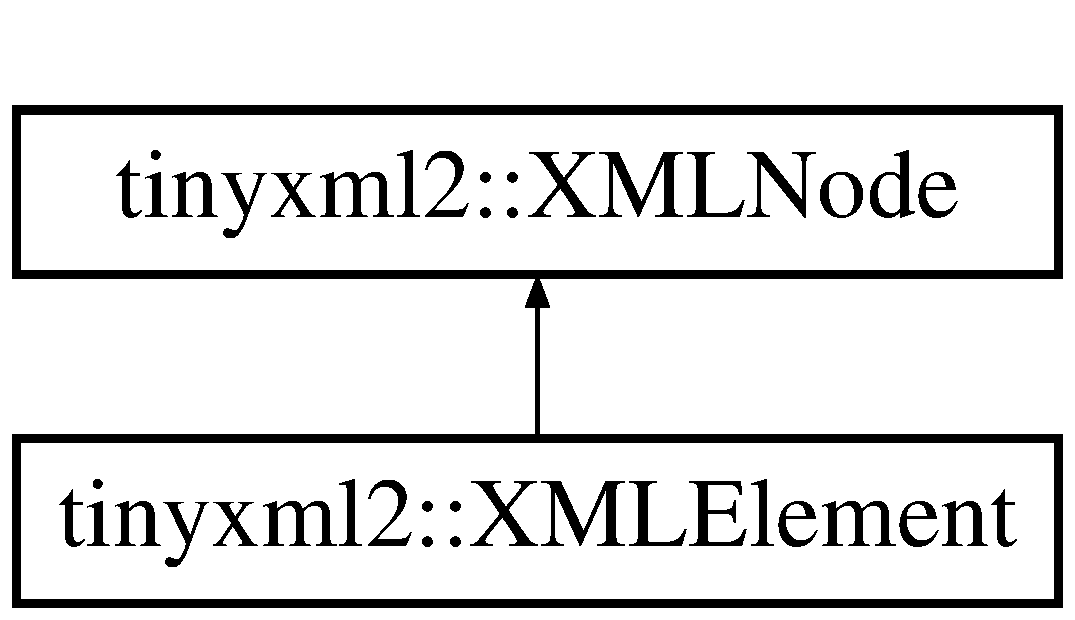
\includegraphics[height=2.000000cm]{classtinyxml2_1_1_x_m_l_element}
\end{center}
\end{figure}
\subsection*{Public Types}
\begin{DoxyCompactItemize}
\item 
enum \{ \hyperlink{classtinyxml2_1_1_x_m_l_element_a07a6ce25c17aaa505933db57f2373e50a78cf277c55b4655c86458dfecb11d349}{O\+P\+EN}, 
\hyperlink{classtinyxml2_1_1_x_m_l_element_a07a6ce25c17aaa505933db57f2373e50aa2f1f384020d2d4538ad2ec84930a028}{C\+L\+O\+S\+ED}, 
\hyperlink{classtinyxml2_1_1_x_m_l_element_a07a6ce25c17aaa505933db57f2373e50aa2857344b98a931536c443cd0cadc4b7}{C\+L\+O\+S\+I\+NG}
 \}
\end{DoxyCompactItemize}
\subsection*{Public Member Functions}
\begin{DoxyCompactItemize}
\item 
const char $\ast$ \hyperlink{classtinyxml2_1_1_x_m_l_element_a63e057fb5baee1dd29f323cb85907b35}{Name} () const
\begin{DoxyCompactList}\small\item\em Get the name of an element (which is the \hyperlink{classtinyxml2_1_1_x_m_l_node_a0485e51c670e741884cfd8362274d680}{Value()} of the node.) \end{DoxyCompactList}\item 
void \hyperlink{classtinyxml2_1_1_x_m_l_element_a97712009a530d8cb8a63bf705f02b4f1}{Set\+Name} (const char $\ast$str, bool static\+Mem=false)
\begin{DoxyCompactList}\small\item\em Set the name of the element. \end{DoxyCompactList}\item 
virtual \hyperlink{classtinyxml2_1_1_x_m_l_element}{X\+M\+L\+Element} $\ast$ \hyperlink{classtinyxml2_1_1_x_m_l_element_ad9ff5c2dbc15df36cf664ce1b0ea0a5d}{To\+Element} ()
\begin{DoxyCompactList}\small\item\em Safely cast to an Element, or null. \end{DoxyCompactList}\item 
virtual const \hyperlink{classtinyxml2_1_1_x_m_l_element}{X\+M\+L\+Element} $\ast$ \hyperlink{classtinyxml2_1_1_x_m_l_element_afeb353047ab8532191709dcaef07337e}{To\+Element} () const
\item 
virtual bool \hyperlink{classtinyxml2_1_1_x_m_l_element_a9b2119831e8b85827d5d3e5076788e4a}{Accept} (\hyperlink{classtinyxml2_1_1_x_m_l_visitor}{X\+M\+L\+Visitor} $\ast$visitor) const
\item 
const char $\ast$ \hyperlink{classtinyxml2_1_1_x_m_l_element_a48cf4a315cfbac7d74cd0d5ff2c5df51}{Attribute} (const char $\ast$name, const char $\ast$value=0) const
\item 
int \hyperlink{classtinyxml2_1_1_x_m_l_element_a95a89b13bb14a2d4655e2b5b406c00d4}{Int\+Attribute} (const char $\ast$name, int default\+Value=0) const
\item 
unsigned \hyperlink{classtinyxml2_1_1_x_m_l_element_afea43a1d4aa33e3703ddee5fc9adc26c}{Unsigned\+Attribute} (const char $\ast$name, unsigned default\+Value=0) const
\begin{DoxyCompactList}\small\item\em See \hyperlink{classtinyxml2_1_1_x_m_l_element_a95a89b13bb14a2d4655e2b5b406c00d4}{Int\+Attribute()} \end{DoxyCompactList}\item 
int64\+\_\+t \hyperlink{classtinyxml2_1_1_x_m_l_element_a66d96972adecd816194191f13cc4a0a0}{Int64\+Attribute} (const char $\ast$name, int64\+\_\+t default\+Value=0) const
\begin{DoxyCompactList}\small\item\em See \hyperlink{classtinyxml2_1_1_x_m_l_element_a95a89b13bb14a2d4655e2b5b406c00d4}{Int\+Attribute()} \end{DoxyCompactList}\item 
bool \hyperlink{classtinyxml2_1_1_x_m_l_element_a53eda26131e1ad1031ef8ec8adb51bd8}{Bool\+Attribute} (const char $\ast$name, bool default\+Value=false) const
\begin{DoxyCompactList}\small\item\em See \hyperlink{classtinyxml2_1_1_x_m_l_element_a95a89b13bb14a2d4655e2b5b406c00d4}{Int\+Attribute()} \end{DoxyCompactList}\item 
double \hyperlink{classtinyxml2_1_1_x_m_l_element_a10a90c505aea716bf073eea1c97f33b5}{Double\+Attribute} (const char $\ast$name, double default\+Value=0) const
\begin{DoxyCompactList}\small\item\em See \hyperlink{classtinyxml2_1_1_x_m_l_element_a95a89b13bb14a2d4655e2b5b406c00d4}{Int\+Attribute()} \end{DoxyCompactList}\item 
float \hyperlink{classtinyxml2_1_1_x_m_l_element_ab1f4be2332e27dc640e9b6abd01d64dd}{Float\+Attribute} (const char $\ast$name, float default\+Value=0) const
\begin{DoxyCompactList}\small\item\em See \hyperlink{classtinyxml2_1_1_x_m_l_element_a95a89b13bb14a2d4655e2b5b406c00d4}{Int\+Attribute()} \end{DoxyCompactList}\item 
\hyperlink{namespacetinyxml2_a1fbf88509c3ac88c09117b1947414e08}{X\+M\+L\+Error} \hyperlink{classtinyxml2_1_1_x_m_l_element_a8a78bc1187c1c45ad89f2690eab567b1}{Query\+Int\+Attribute} (const char $\ast$name, int $\ast$value) const
\item 
\hyperlink{namespacetinyxml2_a1fbf88509c3ac88c09117b1947414e08}{X\+M\+L\+Error} \hyperlink{classtinyxml2_1_1_x_m_l_element_a26fc84cbfba6769dafcfbf256c05e22f}{Query\+Unsigned\+Attribute} (const char $\ast$name, unsigned int $\ast$value) const
\begin{DoxyCompactList}\small\item\em See \hyperlink{classtinyxml2_1_1_x_m_l_element_a8a78bc1187c1c45ad89f2690eab567b1}{Query\+Int\+Attribute()} \end{DoxyCompactList}\item 
\hyperlink{namespacetinyxml2_a1fbf88509c3ac88c09117b1947414e08}{X\+M\+L\+Error} \hyperlink{classtinyxml2_1_1_x_m_l_element_a7c0955d80b6f8d196744eacb0f6e90a8}{Query\+Int64\+Attribute} (const char $\ast$name, int64\+\_\+t $\ast$value) const
\begin{DoxyCompactList}\small\item\em See \hyperlink{classtinyxml2_1_1_x_m_l_element_a8a78bc1187c1c45ad89f2690eab567b1}{Query\+Int\+Attribute()} \end{DoxyCompactList}\item 
\hyperlink{namespacetinyxml2_a1fbf88509c3ac88c09117b1947414e08}{X\+M\+L\+Error} \hyperlink{classtinyxml2_1_1_x_m_l_element_a14c1bb77c39689838be01838d86ca872}{Query\+Bool\+Attribute} (const char $\ast$name, bool $\ast$value) const
\begin{DoxyCompactList}\small\item\em See \hyperlink{classtinyxml2_1_1_x_m_l_element_a8a78bc1187c1c45ad89f2690eab567b1}{Query\+Int\+Attribute()} \end{DoxyCompactList}\item 
\hyperlink{namespacetinyxml2_a1fbf88509c3ac88c09117b1947414e08}{X\+M\+L\+Error} \hyperlink{classtinyxml2_1_1_x_m_l_element_a5f0964e2dbd8e2ee7fce9beab689443c}{Query\+Double\+Attribute} (const char $\ast$name, double $\ast$value) const
\begin{DoxyCompactList}\small\item\em See \hyperlink{classtinyxml2_1_1_x_m_l_element_a8a78bc1187c1c45ad89f2690eab567b1}{Query\+Int\+Attribute()} \end{DoxyCompactList}\item 
\hyperlink{namespacetinyxml2_a1fbf88509c3ac88c09117b1947414e08}{X\+M\+L\+Error} \hyperlink{classtinyxml2_1_1_x_m_l_element_acd5eeddf6002ef90806af794b9d9a5a5}{Query\+Float\+Attribute} (const char $\ast$name, float $\ast$value) const
\begin{DoxyCompactList}\small\item\em See \hyperlink{classtinyxml2_1_1_x_m_l_element_a8a78bc1187c1c45ad89f2690eab567b1}{Query\+Int\+Attribute()} \end{DoxyCompactList}\item 
int \hyperlink{classtinyxml2_1_1_x_m_l_element_a042fc30504347b84a56cf863ad528a4f}{Query\+Attribute} (const char $\ast$name, int $\ast$value) const
\item 
int \hyperlink{classtinyxml2_1_1_x_m_l_element_a187e8b686fbe071732aea2e2ee766f86}{Query\+Attribute} (const char $\ast$name, unsigned int $\ast$value) const
\item 
int \hyperlink{classtinyxml2_1_1_x_m_l_element_aedcac9a0842cc9fcb49ba6eee4dd47bc}{Query\+Attribute} (const char $\ast$name, int64\+\_\+t $\ast$value) const
\item 
int \hyperlink{classtinyxml2_1_1_x_m_l_element_a9aa67feb0392ead13a66f5ea55e71f64}{Query\+Attribute} (const char $\ast$name, bool $\ast$value) const
\item 
int \hyperlink{classtinyxml2_1_1_x_m_l_element_a7f37582f3ad9f9a765e6fa349dfbdfa0}{Query\+Attribute} (const char $\ast$name, double $\ast$value) const
\item 
int \hyperlink{classtinyxml2_1_1_x_m_l_element_a493b6dace830e4dba7110b1e9f6bebd5}{Query\+Attribute} (const char $\ast$name, float $\ast$value) const
\item 
void \hyperlink{classtinyxml2_1_1_x_m_l_element_a11943abf2d0831548c3790dd5d9f119c}{Set\+Attribute} (const char $\ast$name, const char $\ast$value)
\begin{DoxyCompactList}\small\item\em Sets the named attribute to value. \end{DoxyCompactList}\item 
void \hyperlink{classtinyxml2_1_1_x_m_l_element_aae6568c64c7f1cc88be8461ba41a79cf}{Set\+Attribute} (const char $\ast$name, int value)
\begin{DoxyCompactList}\small\item\em Sets the named attribute to value. \end{DoxyCompactList}\item 
void \hyperlink{classtinyxml2_1_1_x_m_l_element_ae143997e90064ba82326b29a9930ea8f}{Set\+Attribute} (const char $\ast$name, unsigned value)
\begin{DoxyCompactList}\small\item\em Sets the named attribute to value. \end{DoxyCompactList}\item 
void \hyperlink{classtinyxml2_1_1_x_m_l_element_aaeefdf9171fec91b13a776b42299b0dd}{Set\+Attribute} (const char $\ast$name, int64\+\_\+t value)
\begin{DoxyCompactList}\small\item\em Sets the named attribute to value. \end{DoxyCompactList}\item 
void \hyperlink{classtinyxml2_1_1_x_m_l_element_aa848b696e6a75e4e545c6da9893b11e1}{Set\+Attribute} (const char $\ast$name, bool value)
\begin{DoxyCompactList}\small\item\em Sets the named attribute to value. \end{DoxyCompactList}\item 
void \hyperlink{classtinyxml2_1_1_x_m_l_element_a233397ee81e70eb5d4b814c5f8698533}{Set\+Attribute} (const char $\ast$name, double value)
\begin{DoxyCompactList}\small\item\em Sets the named attribute to value. \end{DoxyCompactList}\item 
void \hyperlink{classtinyxml2_1_1_x_m_l_element_a554b70d882e65b28fc084b23df9b9759}{Set\+Attribute} (const char $\ast$name, float value)
\begin{DoxyCompactList}\small\item\em Sets the named attribute to value. \end{DoxyCompactList}\item 
void \hyperlink{classtinyxml2_1_1_x_m_l_element_aebd45aa7118964c30b32fe12e944628a}{Delete\+Attribute} (const char $\ast$name)
\item 
const \hyperlink{classtinyxml2_1_1_x_m_l_attribute}{X\+M\+L\+Attribute} $\ast$ \hyperlink{classtinyxml2_1_1_x_m_l_element_a3e191704c8d499906ec11fe2f60c6686}{First\+Attribute} () const
\begin{DoxyCompactList}\small\item\em Return the first attribute in the list. \end{DoxyCompactList}\item 
const \hyperlink{classtinyxml2_1_1_x_m_l_attribute}{X\+M\+L\+Attribute} $\ast$ \hyperlink{classtinyxml2_1_1_x_m_l_element_a157750dac8037a316fd1af1a973dfa2c}{Find\+Attribute} (const char $\ast$name) const
\begin{DoxyCompactList}\small\item\em Query a specific attribute in the list. \end{DoxyCompactList}\item 
const char $\ast$ \hyperlink{classtinyxml2_1_1_x_m_l_element_a0fa5bea0a4daf3ddd503dcabb823eba6}{Get\+Text} () const
\item 
void \hyperlink{classtinyxml2_1_1_x_m_l_element_a1f9c2cd61b72af5ae708d37b7ad283ce}{Set\+Text} (const char $\ast$in\+Text)
\item 
void \hyperlink{classtinyxml2_1_1_x_m_l_element_aeae8917b5ea6060b3c08d4e3d8d632d7}{Set\+Text} (int value)
\begin{DoxyCompactList}\small\item\em Convenience method for setting text inside an element. See \hyperlink{classtinyxml2_1_1_x_m_l_element_a1f9c2cd61b72af5ae708d37b7ad283ce}{Set\+Text()} for important limitations. \end{DoxyCompactList}\item 
void \hyperlink{classtinyxml2_1_1_x_m_l_element_a7bbfcc11d516598bc924a8fba4d08597}{Set\+Text} (unsigned value)
\begin{DoxyCompactList}\small\item\em Convenience method for setting text inside an element. See \hyperlink{classtinyxml2_1_1_x_m_l_element_a1f9c2cd61b72af5ae708d37b7ad283ce}{Set\+Text()} for important limitations. \end{DoxyCompactList}\item 
void \hyperlink{classtinyxml2_1_1_x_m_l_element_a7b62cd33acdfeff7ea2b1b330d4368e4}{Set\+Text} (int64\+\_\+t value)
\begin{DoxyCompactList}\small\item\em Convenience method for setting text inside an element. See \hyperlink{classtinyxml2_1_1_x_m_l_element_a1f9c2cd61b72af5ae708d37b7ad283ce}{Set\+Text()} for important limitations. \end{DoxyCompactList}\item 
void \hyperlink{classtinyxml2_1_1_x_m_l_element_ae4b543d6770de76fb6ab68e541c192a4}{Set\+Text} (bool value)
\begin{DoxyCompactList}\small\item\em Convenience method for setting text inside an element. See \hyperlink{classtinyxml2_1_1_x_m_l_element_a1f9c2cd61b72af5ae708d37b7ad283ce}{Set\+Text()} for important limitations. \end{DoxyCompactList}\item 
void \hyperlink{classtinyxml2_1_1_x_m_l_element_a67bd77ac9aaeff58ff20b4275a65ba4e}{Set\+Text} (double value)
\begin{DoxyCompactList}\small\item\em Convenience method for setting text inside an element. See \hyperlink{classtinyxml2_1_1_x_m_l_element_a1f9c2cd61b72af5ae708d37b7ad283ce}{Set\+Text()} for important limitations. \end{DoxyCompactList}\item 
void \hyperlink{classtinyxml2_1_1_x_m_l_element_a51d560da5ae3ad6b75e0ab9ffb2ae42a}{Set\+Text} (float value)
\begin{DoxyCompactList}\small\item\em Convenience method for setting text inside an element. See \hyperlink{classtinyxml2_1_1_x_m_l_element_a1f9c2cd61b72af5ae708d37b7ad283ce}{Set\+Text()} for important limitations. \end{DoxyCompactList}\item 
\hyperlink{namespacetinyxml2_a1fbf88509c3ac88c09117b1947414e08}{X\+M\+L\+Error} \hyperlink{classtinyxml2_1_1_x_m_l_element_a926357996bef633cb736e1a558419632}{Query\+Int\+Text} (int $\ast$ival) const
\item 
\hyperlink{namespacetinyxml2_a1fbf88509c3ac88c09117b1947414e08}{X\+M\+L\+Error} \hyperlink{classtinyxml2_1_1_x_m_l_element_a14d38aa4b5e18a46274a27425188a6a1}{Query\+Unsigned\+Text} (unsigned $\ast$uval) const
\begin{DoxyCompactList}\small\item\em See \hyperlink{classtinyxml2_1_1_x_m_l_element_a926357996bef633cb736e1a558419632}{Query\+Int\+Text()} \end{DoxyCompactList}\item 
\hyperlink{namespacetinyxml2_a1fbf88509c3ac88c09117b1947414e08}{X\+M\+L\+Error} \hyperlink{classtinyxml2_1_1_x_m_l_element_a120c538c8eead169e635dbc70fb226d8}{Query\+Int64\+Text} (int64\+\_\+t $\ast$uval) const
\begin{DoxyCompactList}\small\item\em See \hyperlink{classtinyxml2_1_1_x_m_l_element_a926357996bef633cb736e1a558419632}{Query\+Int\+Text()} \end{DoxyCompactList}\item 
\hyperlink{namespacetinyxml2_a1fbf88509c3ac88c09117b1947414e08}{X\+M\+L\+Error} \hyperlink{classtinyxml2_1_1_x_m_l_element_a3fe5417d59eb8f5c4afe924b7d332736}{Query\+Bool\+Text} (bool $\ast$bval) const
\begin{DoxyCompactList}\small\item\em See \hyperlink{classtinyxml2_1_1_x_m_l_element_a926357996bef633cb736e1a558419632}{Query\+Int\+Text()} \end{DoxyCompactList}\item 
\hyperlink{namespacetinyxml2_a1fbf88509c3ac88c09117b1947414e08}{X\+M\+L\+Error} \hyperlink{classtinyxml2_1_1_x_m_l_element_a684679c99bb036a25652744cec6c4d96}{Query\+Double\+Text} (double $\ast$dval) const
\begin{DoxyCompactList}\small\item\em See \hyperlink{classtinyxml2_1_1_x_m_l_element_a926357996bef633cb736e1a558419632}{Query\+Int\+Text()} \end{DoxyCompactList}\item 
\hyperlink{namespacetinyxml2_a1fbf88509c3ac88c09117b1947414e08}{X\+M\+L\+Error} \hyperlink{classtinyxml2_1_1_x_m_l_element_afa332afedd93210daa6d44b88eb11e29}{Query\+Float\+Text} (float $\ast$fval) const
\begin{DoxyCompactList}\small\item\em See \hyperlink{classtinyxml2_1_1_x_m_l_element_a926357996bef633cb736e1a558419632}{Query\+Int\+Text()} \end{DoxyCompactList}\item 
int \hyperlink{classtinyxml2_1_1_x_m_l_element_a37b0636adebb8a1a1bc965f60824cb3e}{Int\+Text} (int default\+Value=0) const
\item 
unsigned \hyperlink{classtinyxml2_1_1_x_m_l_element_a49bad014ffcc17b0b6119d5b2c97dfb5}{Unsigned\+Text} (unsigned default\+Value=0) const
\begin{DoxyCompactList}\small\item\em See \hyperlink{classtinyxml2_1_1_x_m_l_element_a926357996bef633cb736e1a558419632}{Query\+Int\+Text()} \end{DoxyCompactList}\item 
int64\+\_\+t \hyperlink{classtinyxml2_1_1_x_m_l_element_aab6151f7e3b4c2c0a8234e262d7b6b8a}{Int64\+Text} (int64\+\_\+t default\+Value=0) const
\begin{DoxyCompactList}\small\item\em See \hyperlink{classtinyxml2_1_1_x_m_l_element_a926357996bef633cb736e1a558419632}{Query\+Int\+Text()} \end{DoxyCompactList}\item 
bool \hyperlink{classtinyxml2_1_1_x_m_l_element_a68569f59f6382bcea7f5013ec59736d2}{Bool\+Text} (bool default\+Value=false) const
\begin{DoxyCompactList}\small\item\em See \hyperlink{classtinyxml2_1_1_x_m_l_element_a926357996bef633cb736e1a558419632}{Query\+Int\+Text()} \end{DoxyCompactList}\item 
double \hyperlink{classtinyxml2_1_1_x_m_l_element_a81b1ff0cf2f2cd09be8badc08b39a2b7}{Double\+Text} (double default\+Value=0) const
\begin{DoxyCompactList}\small\item\em See \hyperlink{classtinyxml2_1_1_x_m_l_element_a926357996bef633cb736e1a558419632}{Query\+Int\+Text()} \end{DoxyCompactList}\item 
float \hyperlink{classtinyxml2_1_1_x_m_l_element_a45444eb21f99ca46101545992dc2e927}{Float\+Text} (float default\+Value=0) const
\begin{DoxyCompactList}\small\item\em See \hyperlink{classtinyxml2_1_1_x_m_l_element_a926357996bef633cb736e1a558419632}{Query\+Int\+Text()} \end{DoxyCompactList}\item 
int \hyperlink{classtinyxml2_1_1_x_m_l_element_ac820806b6c14af6833dcbcf0957b6d61}{Closing\+Type} () const
\item 
virtual \hyperlink{classtinyxml2_1_1_x_m_l_node}{X\+M\+L\+Node} $\ast$ \hyperlink{classtinyxml2_1_1_x_m_l_element_aafa2807a45b28fe096b29d76e6a13b7c}{Shallow\+Clone} (\hyperlink{classtinyxml2_1_1_x_m_l_document}{X\+M\+L\+Document} $\ast$document) const
\item 
virtual bool \hyperlink{classtinyxml2_1_1_x_m_l_element_a61ffd7bf918a9db4aa6203d855ac5ec2}{Shallow\+Equal} (const \hyperlink{classtinyxml2_1_1_x_m_l_node}{X\+M\+L\+Node} $\ast$compare) const
\end{DoxyCompactItemize}
\subsection*{Protected Member Functions}
\begin{DoxyCompactItemize}
\item 
char $\ast$ \hyperlink{classtinyxml2_1_1_x_m_l_element_a0b300321c15576ec02a78422c3796a13}{Parse\+Deep} (char $\ast$p, \hyperlink{classtinyxml2_1_1_str_pair}{Str\+Pair} $\ast$end\+Tag, int $\ast$cur\+Line\+Num\+Ptr)
\end{DoxyCompactItemize}
\subsection*{Friends}
\begin{DoxyCompactItemize}
\item 
class \hyperlink{classtinyxml2_1_1_x_m_l_element_a4eee3bda60c60a30e4e8cd4ea91c4c6e}{X\+M\+L\+Document}
\end{DoxyCompactItemize}
\subsection*{Additional Inherited Members}


\subsection{Detailed Description}
The element is a container class. It has a value, the element name, and can contain other elements, text, comments, and unknowns. Elements also contain an arbitrary number of attributes. 

\subsection{Member Enumeration Documentation}
\mbox{\Hypertarget{classtinyxml2_1_1_x_m_l_element_a07a6ce25c17aaa505933db57f2373e50}\label{classtinyxml2_1_1_x_m_l_element_a07a6ce25c17aaa505933db57f2373e50}} 
\subsubsection{\texorpdfstring{anonymous enum}{anonymous enum}}
{\footnotesize\ttfamily anonymous enum}

\begin{DoxyEnumFields}{Enumerator}
\raisebox{\heightof{T}}[0pt][0pt]{\index{O\+P\+EN@{O\+P\+EN}!tinyxml2\+::\+X\+M\+L\+Element@{tinyxml2\+::\+X\+M\+L\+Element}}\index{tinyxml2\+::\+X\+M\+L\+Element@{tinyxml2\+::\+X\+M\+L\+Element}!O\+P\+EN@{O\+P\+EN}}}\mbox{\Hypertarget{classtinyxml2_1_1_x_m_l_element_a07a6ce25c17aaa505933db57f2373e50a78cf277c55b4655c86458dfecb11d349}\label{classtinyxml2_1_1_x_m_l_element_a07a6ce25c17aaa505933db57f2373e50a78cf277c55b4655c86458dfecb11d349}} 
O\+P\+EN&\\
\hline

\raisebox{\heightof{T}}[0pt][0pt]{\index{C\+L\+O\+S\+ED@{C\+L\+O\+S\+ED}!tinyxml2\+::\+X\+M\+L\+Element@{tinyxml2\+::\+X\+M\+L\+Element}}\index{tinyxml2\+::\+X\+M\+L\+Element@{tinyxml2\+::\+X\+M\+L\+Element}!C\+L\+O\+S\+ED@{C\+L\+O\+S\+ED}}}\mbox{\Hypertarget{classtinyxml2_1_1_x_m_l_element_a07a6ce25c17aaa505933db57f2373e50aa2f1f384020d2d4538ad2ec84930a028}\label{classtinyxml2_1_1_x_m_l_element_a07a6ce25c17aaa505933db57f2373e50aa2f1f384020d2d4538ad2ec84930a028}} 
C\+L\+O\+S\+ED&\\
\hline

\raisebox{\heightof{T}}[0pt][0pt]{\index{C\+L\+O\+S\+I\+NG@{C\+L\+O\+S\+I\+NG}!tinyxml2\+::\+X\+M\+L\+Element@{tinyxml2\+::\+X\+M\+L\+Element}}\index{tinyxml2\+::\+X\+M\+L\+Element@{tinyxml2\+::\+X\+M\+L\+Element}!C\+L\+O\+S\+I\+NG@{C\+L\+O\+S\+I\+NG}}}\mbox{\Hypertarget{classtinyxml2_1_1_x_m_l_element_a07a6ce25c17aaa505933db57f2373e50aa2857344b98a931536c443cd0cadc4b7}\label{classtinyxml2_1_1_x_m_l_element_a07a6ce25c17aaa505933db57f2373e50aa2857344b98a931536c443cd0cadc4b7}} 
C\+L\+O\+S\+I\+NG&\\
\hline

\end{DoxyEnumFields}


\subsection{Member Function Documentation}
\mbox{\Hypertarget{classtinyxml2_1_1_x_m_l_element_a9b2119831e8b85827d5d3e5076788e4a}\label{classtinyxml2_1_1_x_m_l_element_a9b2119831e8b85827d5d3e5076788e4a}} 
\index{tinyxml2\+::\+X\+M\+L\+Element@{tinyxml2\+::\+X\+M\+L\+Element}!Accept@{Accept}}
\index{Accept@{Accept}!tinyxml2\+::\+X\+M\+L\+Element@{tinyxml2\+::\+X\+M\+L\+Element}}
\subsubsection{\texorpdfstring{Accept()}{Accept()}}
{\footnotesize\ttfamily bool tinyxml2\+::\+X\+M\+L\+Element\+::\+Accept (\begin{DoxyParamCaption}\item[{\hyperlink{classtinyxml2_1_1_x_m_l_visitor}{X\+M\+L\+Visitor} $\ast$}]{visitor }\end{DoxyParamCaption}) const\hspace{0.3cm}{\ttfamily [virtual]}}

Accept a hierarchical visit of the nodes in the Tiny\+X\+M\+L-\/2 D\+OM. Every node in the X\+ML tree will be conditionally visited and the host will be called back via the \hyperlink{classtinyxml2_1_1_x_m_l_visitor}{X\+M\+L\+Visitor} interface.

This is essentially a S\+AX interface for Tiny\+X\+M\+L-\/2. (Note however it doesn\textquotesingle{}t re-\/parse the X\+ML for the callbacks, so the performance of Tiny\+X\+M\+L-\/2 is unchanged by using this interface versus any other.)

The interface has been based on ideas from\+:


\begin{DoxyItemize}
\item \href{http://www.saxproject.org/}{\tt http\+://www.\+saxproject.\+org/}
\item \href{http://c2.com/cgi/wiki?HierarchicalVisitorPattern}{\tt http\+://c2.\+com/cgi/wiki?\+Hierarchical\+Visitor\+Pattern}
\end{DoxyItemize}

Which are both good references for \char`\"{}visiting\char`\"{}.

An example of using \hyperlink{classtinyxml2_1_1_x_m_l_element_a9b2119831e8b85827d5d3e5076788e4a}{Accept()}\+: \begin{DoxyVerb}XMLPrinter printer;
tinyxmlDoc.Accept( &printer );
const char* xmlcstr = printer.CStr();
\end{DoxyVerb}
 

Implements \hyperlink{classtinyxml2_1_1_x_m_l_node_a81e66df0a44c67a7af17f3b77a152785}{tinyxml2\+::\+X\+M\+L\+Node}.

\mbox{\Hypertarget{classtinyxml2_1_1_x_m_l_element_a48cf4a315cfbac7d74cd0d5ff2c5df51}\label{classtinyxml2_1_1_x_m_l_element_a48cf4a315cfbac7d74cd0d5ff2c5df51}} 
\index{tinyxml2\+::\+X\+M\+L\+Element@{tinyxml2\+::\+X\+M\+L\+Element}!Attribute@{Attribute}}
\index{Attribute@{Attribute}!tinyxml2\+::\+X\+M\+L\+Element@{tinyxml2\+::\+X\+M\+L\+Element}}
\subsubsection{\texorpdfstring{Attribute()}{Attribute()}}
{\footnotesize\ttfamily const char $\ast$ tinyxml2\+::\+X\+M\+L\+Element\+::\+Attribute (\begin{DoxyParamCaption}\item[{const char $\ast$}]{name,  }\item[{const char $\ast$}]{value = {\ttfamily 0} }\end{DoxyParamCaption}) const}

Given an attribute name, \hyperlink{classtinyxml2_1_1_x_m_l_element_a48cf4a315cfbac7d74cd0d5ff2c5df51}{Attribute()} returns the value for the attribute of that name, or null if none exists. For example\+:

\begin{DoxyVerb}const char* value = ele->Attribute( "foo" );
\end{DoxyVerb}


The \textquotesingle{}value\textquotesingle{} parameter is normally null. However, if specified, the attribute will only be returned if the \textquotesingle{}name\textquotesingle{} and \textquotesingle{}value\textquotesingle{} match. This allow you to write code\+:

\begin{DoxyVerb}if ( ele->Attribute( "foo", "bar" ) ) callFooIsBar();
\end{DoxyVerb}


rather than\+: \begin{DoxyVerb}if ( ele->Attribute( "foo" ) ) {
if ( strcmp( ele->Attribute( "foo" ), "bar" ) == 0 ) callFooIsBar();
}
\end{DoxyVerb}
 \mbox{\Hypertarget{classtinyxml2_1_1_x_m_l_element_a53eda26131e1ad1031ef8ec8adb51bd8}\label{classtinyxml2_1_1_x_m_l_element_a53eda26131e1ad1031ef8ec8adb51bd8}} 
\index{tinyxml2\+::\+X\+M\+L\+Element@{tinyxml2\+::\+X\+M\+L\+Element}!Bool\+Attribute@{Bool\+Attribute}}
\index{Bool\+Attribute@{Bool\+Attribute}!tinyxml2\+::\+X\+M\+L\+Element@{tinyxml2\+::\+X\+M\+L\+Element}}
\subsubsection{\texorpdfstring{Bool\+Attribute()}{BoolAttribute()}}
{\footnotesize\ttfamily bool tinyxml2\+::\+X\+M\+L\+Element\+::\+Bool\+Attribute (\begin{DoxyParamCaption}\item[{const char $\ast$}]{name,  }\item[{bool}]{default\+Value = {\ttfamily false} }\end{DoxyParamCaption}) const}



See \hyperlink{classtinyxml2_1_1_x_m_l_element_a95a89b13bb14a2d4655e2b5b406c00d4}{Int\+Attribute()} 

\mbox{\Hypertarget{classtinyxml2_1_1_x_m_l_element_a68569f59f6382bcea7f5013ec59736d2}\label{classtinyxml2_1_1_x_m_l_element_a68569f59f6382bcea7f5013ec59736d2}} 
\index{tinyxml2\+::\+X\+M\+L\+Element@{tinyxml2\+::\+X\+M\+L\+Element}!Bool\+Text@{Bool\+Text}}
\index{Bool\+Text@{Bool\+Text}!tinyxml2\+::\+X\+M\+L\+Element@{tinyxml2\+::\+X\+M\+L\+Element}}
\subsubsection{\texorpdfstring{Bool\+Text()}{BoolText()}}
{\footnotesize\ttfamily bool tinyxml2\+::\+X\+M\+L\+Element\+::\+Bool\+Text (\begin{DoxyParamCaption}\item[{bool}]{default\+Value = {\ttfamily false} }\end{DoxyParamCaption}) const}



See \hyperlink{classtinyxml2_1_1_x_m_l_element_a926357996bef633cb736e1a558419632}{Query\+Int\+Text()} 

\mbox{\Hypertarget{classtinyxml2_1_1_x_m_l_element_ac820806b6c14af6833dcbcf0957b6d61}\label{classtinyxml2_1_1_x_m_l_element_ac820806b6c14af6833dcbcf0957b6d61}} 
\index{tinyxml2\+::\+X\+M\+L\+Element@{tinyxml2\+::\+X\+M\+L\+Element}!Closing\+Type@{Closing\+Type}}
\index{Closing\+Type@{Closing\+Type}!tinyxml2\+::\+X\+M\+L\+Element@{tinyxml2\+::\+X\+M\+L\+Element}}
\subsubsection{\texorpdfstring{Closing\+Type()}{ClosingType()}}
{\footnotesize\ttfamily int tinyxml2\+::\+X\+M\+L\+Element\+::\+Closing\+Type (\begin{DoxyParamCaption}{ }\end{DoxyParamCaption}) const\hspace{0.3cm}{\ttfamily [inline]}}

\mbox{\Hypertarget{classtinyxml2_1_1_x_m_l_element_aebd45aa7118964c30b32fe12e944628a}\label{classtinyxml2_1_1_x_m_l_element_aebd45aa7118964c30b32fe12e944628a}} 
\index{tinyxml2\+::\+X\+M\+L\+Element@{tinyxml2\+::\+X\+M\+L\+Element}!Delete\+Attribute@{Delete\+Attribute}}
\index{Delete\+Attribute@{Delete\+Attribute}!tinyxml2\+::\+X\+M\+L\+Element@{tinyxml2\+::\+X\+M\+L\+Element}}
\subsubsection{\texorpdfstring{Delete\+Attribute()}{DeleteAttribute()}}
{\footnotesize\ttfamily void tinyxml2\+::\+X\+M\+L\+Element\+::\+Delete\+Attribute (\begin{DoxyParamCaption}\item[{const char $\ast$}]{name }\end{DoxyParamCaption})}

Delete an attribute. \mbox{\Hypertarget{classtinyxml2_1_1_x_m_l_element_a10a90c505aea716bf073eea1c97f33b5}\label{classtinyxml2_1_1_x_m_l_element_a10a90c505aea716bf073eea1c97f33b5}} 
\index{tinyxml2\+::\+X\+M\+L\+Element@{tinyxml2\+::\+X\+M\+L\+Element}!Double\+Attribute@{Double\+Attribute}}
\index{Double\+Attribute@{Double\+Attribute}!tinyxml2\+::\+X\+M\+L\+Element@{tinyxml2\+::\+X\+M\+L\+Element}}
\subsubsection{\texorpdfstring{Double\+Attribute()}{DoubleAttribute()}}
{\footnotesize\ttfamily double tinyxml2\+::\+X\+M\+L\+Element\+::\+Double\+Attribute (\begin{DoxyParamCaption}\item[{const char $\ast$}]{name,  }\item[{double}]{default\+Value = {\ttfamily 0} }\end{DoxyParamCaption}) const}



See \hyperlink{classtinyxml2_1_1_x_m_l_element_a95a89b13bb14a2d4655e2b5b406c00d4}{Int\+Attribute()} 

\mbox{\Hypertarget{classtinyxml2_1_1_x_m_l_element_a81b1ff0cf2f2cd09be8badc08b39a2b7}\label{classtinyxml2_1_1_x_m_l_element_a81b1ff0cf2f2cd09be8badc08b39a2b7}} 
\index{tinyxml2\+::\+X\+M\+L\+Element@{tinyxml2\+::\+X\+M\+L\+Element}!Double\+Text@{Double\+Text}}
\index{Double\+Text@{Double\+Text}!tinyxml2\+::\+X\+M\+L\+Element@{tinyxml2\+::\+X\+M\+L\+Element}}
\subsubsection{\texorpdfstring{Double\+Text()}{DoubleText()}}
{\footnotesize\ttfamily double tinyxml2\+::\+X\+M\+L\+Element\+::\+Double\+Text (\begin{DoxyParamCaption}\item[{double}]{default\+Value = {\ttfamily 0} }\end{DoxyParamCaption}) const}



See \hyperlink{classtinyxml2_1_1_x_m_l_element_a926357996bef633cb736e1a558419632}{Query\+Int\+Text()} 

\mbox{\Hypertarget{classtinyxml2_1_1_x_m_l_element_a157750dac8037a316fd1af1a973dfa2c}\label{classtinyxml2_1_1_x_m_l_element_a157750dac8037a316fd1af1a973dfa2c}} 
\index{tinyxml2\+::\+X\+M\+L\+Element@{tinyxml2\+::\+X\+M\+L\+Element}!Find\+Attribute@{Find\+Attribute}}
\index{Find\+Attribute@{Find\+Attribute}!tinyxml2\+::\+X\+M\+L\+Element@{tinyxml2\+::\+X\+M\+L\+Element}}
\subsubsection{\texorpdfstring{Find\+Attribute()}{FindAttribute()}}
{\footnotesize\ttfamily const \hyperlink{classtinyxml2_1_1_x_m_l_attribute}{X\+M\+L\+Attribute} $\ast$ tinyxml2\+::\+X\+M\+L\+Element\+::\+Find\+Attribute (\begin{DoxyParamCaption}\item[{const char $\ast$}]{name }\end{DoxyParamCaption}) const}



Query a specific attribute in the list. 

\mbox{\Hypertarget{classtinyxml2_1_1_x_m_l_element_a3e191704c8d499906ec11fe2f60c6686}\label{classtinyxml2_1_1_x_m_l_element_a3e191704c8d499906ec11fe2f60c6686}} 
\index{tinyxml2\+::\+X\+M\+L\+Element@{tinyxml2\+::\+X\+M\+L\+Element}!First\+Attribute@{First\+Attribute}}
\index{First\+Attribute@{First\+Attribute}!tinyxml2\+::\+X\+M\+L\+Element@{tinyxml2\+::\+X\+M\+L\+Element}}
\subsubsection{\texorpdfstring{First\+Attribute()}{FirstAttribute()}}
{\footnotesize\ttfamily const \hyperlink{classtinyxml2_1_1_x_m_l_attribute}{X\+M\+L\+Attribute}$\ast$ tinyxml2\+::\+X\+M\+L\+Element\+::\+First\+Attribute (\begin{DoxyParamCaption}{ }\end{DoxyParamCaption}) const\hspace{0.3cm}{\ttfamily [inline]}}



Return the first attribute in the list. 

\mbox{\Hypertarget{classtinyxml2_1_1_x_m_l_element_ab1f4be2332e27dc640e9b6abd01d64dd}\label{classtinyxml2_1_1_x_m_l_element_ab1f4be2332e27dc640e9b6abd01d64dd}} 
\index{tinyxml2\+::\+X\+M\+L\+Element@{tinyxml2\+::\+X\+M\+L\+Element}!Float\+Attribute@{Float\+Attribute}}
\index{Float\+Attribute@{Float\+Attribute}!tinyxml2\+::\+X\+M\+L\+Element@{tinyxml2\+::\+X\+M\+L\+Element}}
\subsubsection{\texorpdfstring{Float\+Attribute()}{FloatAttribute()}}
{\footnotesize\ttfamily float tinyxml2\+::\+X\+M\+L\+Element\+::\+Float\+Attribute (\begin{DoxyParamCaption}\item[{const char $\ast$}]{name,  }\item[{float}]{default\+Value = {\ttfamily 0} }\end{DoxyParamCaption}) const}



See \hyperlink{classtinyxml2_1_1_x_m_l_element_a95a89b13bb14a2d4655e2b5b406c00d4}{Int\+Attribute()} 

\mbox{\Hypertarget{classtinyxml2_1_1_x_m_l_element_a45444eb21f99ca46101545992dc2e927}\label{classtinyxml2_1_1_x_m_l_element_a45444eb21f99ca46101545992dc2e927}} 
\index{tinyxml2\+::\+X\+M\+L\+Element@{tinyxml2\+::\+X\+M\+L\+Element}!Float\+Text@{Float\+Text}}
\index{Float\+Text@{Float\+Text}!tinyxml2\+::\+X\+M\+L\+Element@{tinyxml2\+::\+X\+M\+L\+Element}}
\subsubsection{\texorpdfstring{Float\+Text()}{FloatText()}}
{\footnotesize\ttfamily float tinyxml2\+::\+X\+M\+L\+Element\+::\+Float\+Text (\begin{DoxyParamCaption}\item[{float}]{default\+Value = {\ttfamily 0} }\end{DoxyParamCaption}) const}



See \hyperlink{classtinyxml2_1_1_x_m_l_element_a926357996bef633cb736e1a558419632}{Query\+Int\+Text()} 

\mbox{\Hypertarget{classtinyxml2_1_1_x_m_l_element_a0fa5bea0a4daf3ddd503dcabb823eba6}\label{classtinyxml2_1_1_x_m_l_element_a0fa5bea0a4daf3ddd503dcabb823eba6}} 
\index{tinyxml2\+::\+X\+M\+L\+Element@{tinyxml2\+::\+X\+M\+L\+Element}!Get\+Text@{Get\+Text}}
\index{Get\+Text@{Get\+Text}!tinyxml2\+::\+X\+M\+L\+Element@{tinyxml2\+::\+X\+M\+L\+Element}}
\subsubsection{\texorpdfstring{Get\+Text()}{GetText()}}
{\footnotesize\ttfamily const char $\ast$ tinyxml2\+::\+X\+M\+L\+Element\+::\+Get\+Text (\begin{DoxyParamCaption}{ }\end{DoxyParamCaption}) const}

Convenience function for easy access to the text inside an element. Although easy and concise, \hyperlink{classtinyxml2_1_1_x_m_l_element_a0fa5bea0a4daf3ddd503dcabb823eba6}{Get\+Text()} is limited compared to getting the \hyperlink{classtinyxml2_1_1_x_m_l_text}{X\+M\+L\+Text} child and accessing it directly.

If the first child of \textquotesingle{}this\textquotesingle{} is a \hyperlink{classtinyxml2_1_1_x_m_l_text}{X\+M\+L\+Text}, the \hyperlink{classtinyxml2_1_1_x_m_l_element_a0fa5bea0a4daf3ddd503dcabb823eba6}{Get\+Text()} returns the character string of the Text node, else null is returned.

This is a convenient method for getting the text of simple contained text\+: \begin{DoxyVerb}<foo>This is text</foo>
const char* str = fooElement->GetText();
\end{DoxyVerb}


\textquotesingle{}str\textquotesingle{} will be a pointer to \char`\"{}\+This is text\char`\"{}.

Note that this function can be misleading. If the element foo was created from this X\+ML\+: \begin{DoxyVerb}<foo><b>This is text</b></foo>
\end{DoxyVerb}


then the value of str would be null. The first child node isn\textquotesingle{}t a text node, it is another element. From this X\+ML\+: \begin{DoxyVerb}<foo>This is <b>text</b></foo>
\end{DoxyVerb}
 \hyperlink{classtinyxml2_1_1_x_m_l_element_a0fa5bea0a4daf3ddd503dcabb823eba6}{Get\+Text()} will return \char`\"{}\+This is \char`\"{}. \mbox{\Hypertarget{classtinyxml2_1_1_x_m_l_element_a66d96972adecd816194191f13cc4a0a0}\label{classtinyxml2_1_1_x_m_l_element_a66d96972adecd816194191f13cc4a0a0}} 
\index{tinyxml2\+::\+X\+M\+L\+Element@{tinyxml2\+::\+X\+M\+L\+Element}!Int64\+Attribute@{Int64\+Attribute}}
\index{Int64\+Attribute@{Int64\+Attribute}!tinyxml2\+::\+X\+M\+L\+Element@{tinyxml2\+::\+X\+M\+L\+Element}}
\subsubsection{\texorpdfstring{Int64\+Attribute()}{Int64Attribute()}}
{\footnotesize\ttfamily int64\+\_\+t tinyxml2\+::\+X\+M\+L\+Element\+::\+Int64\+Attribute (\begin{DoxyParamCaption}\item[{const char $\ast$}]{name,  }\item[{int64\+\_\+t}]{default\+Value = {\ttfamily 0} }\end{DoxyParamCaption}) const}



See \hyperlink{classtinyxml2_1_1_x_m_l_element_a95a89b13bb14a2d4655e2b5b406c00d4}{Int\+Attribute()} 

\mbox{\Hypertarget{classtinyxml2_1_1_x_m_l_element_aab6151f7e3b4c2c0a8234e262d7b6b8a}\label{classtinyxml2_1_1_x_m_l_element_aab6151f7e3b4c2c0a8234e262d7b6b8a}} 
\index{tinyxml2\+::\+X\+M\+L\+Element@{tinyxml2\+::\+X\+M\+L\+Element}!Int64\+Text@{Int64\+Text}}
\index{Int64\+Text@{Int64\+Text}!tinyxml2\+::\+X\+M\+L\+Element@{tinyxml2\+::\+X\+M\+L\+Element}}
\subsubsection{\texorpdfstring{Int64\+Text()}{Int64Text()}}
{\footnotesize\ttfamily int64\+\_\+t tinyxml2\+::\+X\+M\+L\+Element\+::\+Int64\+Text (\begin{DoxyParamCaption}\item[{int64\+\_\+t}]{default\+Value = {\ttfamily 0} }\end{DoxyParamCaption}) const}



See \hyperlink{classtinyxml2_1_1_x_m_l_element_a926357996bef633cb736e1a558419632}{Query\+Int\+Text()} 

\mbox{\Hypertarget{classtinyxml2_1_1_x_m_l_element_a95a89b13bb14a2d4655e2b5b406c00d4}\label{classtinyxml2_1_1_x_m_l_element_a95a89b13bb14a2d4655e2b5b406c00d4}} 
\index{tinyxml2\+::\+X\+M\+L\+Element@{tinyxml2\+::\+X\+M\+L\+Element}!Int\+Attribute@{Int\+Attribute}}
\index{Int\+Attribute@{Int\+Attribute}!tinyxml2\+::\+X\+M\+L\+Element@{tinyxml2\+::\+X\+M\+L\+Element}}
\subsubsection{\texorpdfstring{Int\+Attribute()}{IntAttribute()}}
{\footnotesize\ttfamily int tinyxml2\+::\+X\+M\+L\+Element\+::\+Int\+Attribute (\begin{DoxyParamCaption}\item[{const char $\ast$}]{name,  }\item[{int}]{default\+Value = {\ttfamily 0} }\end{DoxyParamCaption}) const}

Given an attribute name, \hyperlink{classtinyxml2_1_1_x_m_l_element_a95a89b13bb14a2d4655e2b5b406c00d4}{Int\+Attribute()} returns the value of the attribute interpreted as an integer. The default value will be returned if the attribute isn\textquotesingle{}t present, or if there is an error. (For a method with error checking, see \hyperlink{classtinyxml2_1_1_x_m_l_element_a8a78bc1187c1c45ad89f2690eab567b1}{Query\+Int\+Attribute()}). \mbox{\Hypertarget{classtinyxml2_1_1_x_m_l_element_a37b0636adebb8a1a1bc965f60824cb3e}\label{classtinyxml2_1_1_x_m_l_element_a37b0636adebb8a1a1bc965f60824cb3e}} 
\index{tinyxml2\+::\+X\+M\+L\+Element@{tinyxml2\+::\+X\+M\+L\+Element}!Int\+Text@{Int\+Text}}
\index{Int\+Text@{Int\+Text}!tinyxml2\+::\+X\+M\+L\+Element@{tinyxml2\+::\+X\+M\+L\+Element}}
\subsubsection{\texorpdfstring{Int\+Text()}{IntText()}}
{\footnotesize\ttfamily int tinyxml2\+::\+X\+M\+L\+Element\+::\+Int\+Text (\begin{DoxyParamCaption}\item[{int}]{default\+Value = {\ttfamily 0} }\end{DoxyParamCaption}) const}

\mbox{\Hypertarget{classtinyxml2_1_1_x_m_l_element_a63e057fb5baee1dd29f323cb85907b35}\label{classtinyxml2_1_1_x_m_l_element_a63e057fb5baee1dd29f323cb85907b35}} 
\index{tinyxml2\+::\+X\+M\+L\+Element@{tinyxml2\+::\+X\+M\+L\+Element}!Name@{Name}}
\index{Name@{Name}!tinyxml2\+::\+X\+M\+L\+Element@{tinyxml2\+::\+X\+M\+L\+Element}}
\subsubsection{\texorpdfstring{Name()}{Name()}}
{\footnotesize\ttfamily const char$\ast$ tinyxml2\+::\+X\+M\+L\+Element\+::\+Name (\begin{DoxyParamCaption}{ }\end{DoxyParamCaption}) const\hspace{0.3cm}{\ttfamily [inline]}}



Get the name of an element (which is the \hyperlink{classtinyxml2_1_1_x_m_l_node_a0485e51c670e741884cfd8362274d680}{Value()} of the node.) 

\mbox{\Hypertarget{classtinyxml2_1_1_x_m_l_element_a0b300321c15576ec02a78422c3796a13}\label{classtinyxml2_1_1_x_m_l_element_a0b300321c15576ec02a78422c3796a13}} 
\index{tinyxml2\+::\+X\+M\+L\+Element@{tinyxml2\+::\+X\+M\+L\+Element}!Parse\+Deep@{Parse\+Deep}}
\index{Parse\+Deep@{Parse\+Deep}!tinyxml2\+::\+X\+M\+L\+Element@{tinyxml2\+::\+X\+M\+L\+Element}}
\subsubsection{\texorpdfstring{Parse\+Deep()}{ParseDeep()}}
{\footnotesize\ttfamily char $\ast$ tinyxml2\+::\+X\+M\+L\+Element\+::\+Parse\+Deep (\begin{DoxyParamCaption}\item[{char $\ast$}]{p,  }\item[{\hyperlink{classtinyxml2_1_1_str_pair}{Str\+Pair} $\ast$}]{end\+Tag,  }\item[{int $\ast$}]{cur\+Line\+Num\+Ptr }\end{DoxyParamCaption})\hspace{0.3cm}{\ttfamily [protected]}, {\ttfamily [virtual]}}



Reimplemented from \hyperlink{classtinyxml2_1_1_x_m_l_node_a0afc27892998f31735f6225edb40a40d}{tinyxml2\+::\+X\+M\+L\+Node}.

\mbox{\Hypertarget{classtinyxml2_1_1_x_m_l_element_a042fc30504347b84a56cf863ad528a4f}\label{classtinyxml2_1_1_x_m_l_element_a042fc30504347b84a56cf863ad528a4f}} 
\index{tinyxml2\+::\+X\+M\+L\+Element@{tinyxml2\+::\+X\+M\+L\+Element}!Query\+Attribute@{Query\+Attribute}}
\index{Query\+Attribute@{Query\+Attribute}!tinyxml2\+::\+X\+M\+L\+Element@{tinyxml2\+::\+X\+M\+L\+Element}}
\subsubsection{\texorpdfstring{Query\+Attribute()}{QueryAttribute()}\hspace{0.1cm}{\footnotesize\ttfamily [1/6]}}
{\footnotesize\ttfamily int tinyxml2\+::\+X\+M\+L\+Element\+::\+Query\+Attribute (\begin{DoxyParamCaption}\item[{const char $\ast$}]{name,  }\item[{int $\ast$}]{value }\end{DoxyParamCaption}) const\hspace{0.3cm}{\ttfamily [inline]}}

Given an attribute name, \hyperlink{classtinyxml2_1_1_x_m_l_element_a042fc30504347b84a56cf863ad528a4f}{Query\+Attribute()} returns X\+M\+L\+\_\+\+S\+U\+C\+C\+E\+SS, X\+M\+L\+\_\+\+W\+R\+O\+N\+G\+\_\+\+A\+T\+T\+R\+I\+B\+U\+T\+E\+\_\+\+T\+Y\+PE if the conversion can\textquotesingle{}t be performed, or X\+M\+L\+\_\+\+N\+O\+\_\+\+A\+T\+T\+R\+I\+B\+U\+TE if the attribute doesn\textquotesingle{}t exist. It is overloaded for the primitive types, and is a generally more convenient replacement of \hyperlink{classtinyxml2_1_1_x_m_l_element_a8a78bc1187c1c45ad89f2690eab567b1}{Query\+Int\+Attribute()} and related functions.

If successful, the result of the conversion will be written to \textquotesingle{}value\textquotesingle{}. If not successful, nothing will be written to \textquotesingle{}value\textquotesingle{}. This allows you to provide default value\+:

\begin{DoxyVerb}int value = 10;
QueryAttribute( "foo", &value );        // if "foo" isn't found, value will still be 10
\end{DoxyVerb}
 \mbox{\Hypertarget{classtinyxml2_1_1_x_m_l_element_a187e8b686fbe071732aea2e2ee766f86}\label{classtinyxml2_1_1_x_m_l_element_a187e8b686fbe071732aea2e2ee766f86}} 
\index{tinyxml2\+::\+X\+M\+L\+Element@{tinyxml2\+::\+X\+M\+L\+Element}!Query\+Attribute@{Query\+Attribute}}
\index{Query\+Attribute@{Query\+Attribute}!tinyxml2\+::\+X\+M\+L\+Element@{tinyxml2\+::\+X\+M\+L\+Element}}
\subsubsection{\texorpdfstring{Query\+Attribute()}{QueryAttribute()}\hspace{0.1cm}{\footnotesize\ttfamily [2/6]}}
{\footnotesize\ttfamily int tinyxml2\+::\+X\+M\+L\+Element\+::\+Query\+Attribute (\begin{DoxyParamCaption}\item[{const char $\ast$}]{name,  }\item[{unsigned int $\ast$}]{value }\end{DoxyParamCaption}) const\hspace{0.3cm}{\ttfamily [inline]}}

\mbox{\Hypertarget{classtinyxml2_1_1_x_m_l_element_aedcac9a0842cc9fcb49ba6eee4dd47bc}\label{classtinyxml2_1_1_x_m_l_element_aedcac9a0842cc9fcb49ba6eee4dd47bc}} 
\index{tinyxml2\+::\+X\+M\+L\+Element@{tinyxml2\+::\+X\+M\+L\+Element}!Query\+Attribute@{Query\+Attribute}}
\index{Query\+Attribute@{Query\+Attribute}!tinyxml2\+::\+X\+M\+L\+Element@{tinyxml2\+::\+X\+M\+L\+Element}}
\subsubsection{\texorpdfstring{Query\+Attribute()}{QueryAttribute()}\hspace{0.1cm}{\footnotesize\ttfamily [3/6]}}
{\footnotesize\ttfamily int tinyxml2\+::\+X\+M\+L\+Element\+::\+Query\+Attribute (\begin{DoxyParamCaption}\item[{const char $\ast$}]{name,  }\item[{int64\+\_\+t $\ast$}]{value }\end{DoxyParamCaption}) const\hspace{0.3cm}{\ttfamily [inline]}}

\mbox{\Hypertarget{classtinyxml2_1_1_x_m_l_element_a9aa67feb0392ead13a66f5ea55e71f64}\label{classtinyxml2_1_1_x_m_l_element_a9aa67feb0392ead13a66f5ea55e71f64}} 
\index{tinyxml2\+::\+X\+M\+L\+Element@{tinyxml2\+::\+X\+M\+L\+Element}!Query\+Attribute@{Query\+Attribute}}
\index{Query\+Attribute@{Query\+Attribute}!tinyxml2\+::\+X\+M\+L\+Element@{tinyxml2\+::\+X\+M\+L\+Element}}
\subsubsection{\texorpdfstring{Query\+Attribute()}{QueryAttribute()}\hspace{0.1cm}{\footnotesize\ttfamily [4/6]}}
{\footnotesize\ttfamily int tinyxml2\+::\+X\+M\+L\+Element\+::\+Query\+Attribute (\begin{DoxyParamCaption}\item[{const char $\ast$}]{name,  }\item[{bool $\ast$}]{value }\end{DoxyParamCaption}) const\hspace{0.3cm}{\ttfamily [inline]}}

\mbox{\Hypertarget{classtinyxml2_1_1_x_m_l_element_a7f37582f3ad9f9a765e6fa349dfbdfa0}\label{classtinyxml2_1_1_x_m_l_element_a7f37582f3ad9f9a765e6fa349dfbdfa0}} 
\index{tinyxml2\+::\+X\+M\+L\+Element@{tinyxml2\+::\+X\+M\+L\+Element}!Query\+Attribute@{Query\+Attribute}}
\index{Query\+Attribute@{Query\+Attribute}!tinyxml2\+::\+X\+M\+L\+Element@{tinyxml2\+::\+X\+M\+L\+Element}}
\subsubsection{\texorpdfstring{Query\+Attribute()}{QueryAttribute()}\hspace{0.1cm}{\footnotesize\ttfamily [5/6]}}
{\footnotesize\ttfamily int tinyxml2\+::\+X\+M\+L\+Element\+::\+Query\+Attribute (\begin{DoxyParamCaption}\item[{const char $\ast$}]{name,  }\item[{double $\ast$}]{value }\end{DoxyParamCaption}) const\hspace{0.3cm}{\ttfamily [inline]}}

\mbox{\Hypertarget{classtinyxml2_1_1_x_m_l_element_a493b6dace830e4dba7110b1e9f6bebd5}\label{classtinyxml2_1_1_x_m_l_element_a493b6dace830e4dba7110b1e9f6bebd5}} 
\index{tinyxml2\+::\+X\+M\+L\+Element@{tinyxml2\+::\+X\+M\+L\+Element}!Query\+Attribute@{Query\+Attribute}}
\index{Query\+Attribute@{Query\+Attribute}!tinyxml2\+::\+X\+M\+L\+Element@{tinyxml2\+::\+X\+M\+L\+Element}}
\subsubsection{\texorpdfstring{Query\+Attribute()}{QueryAttribute()}\hspace{0.1cm}{\footnotesize\ttfamily [6/6]}}
{\footnotesize\ttfamily int tinyxml2\+::\+X\+M\+L\+Element\+::\+Query\+Attribute (\begin{DoxyParamCaption}\item[{const char $\ast$}]{name,  }\item[{float $\ast$}]{value }\end{DoxyParamCaption}) const\hspace{0.3cm}{\ttfamily [inline]}}

\mbox{\Hypertarget{classtinyxml2_1_1_x_m_l_element_a14c1bb77c39689838be01838d86ca872}\label{classtinyxml2_1_1_x_m_l_element_a14c1bb77c39689838be01838d86ca872}} 
\index{tinyxml2\+::\+X\+M\+L\+Element@{tinyxml2\+::\+X\+M\+L\+Element}!Query\+Bool\+Attribute@{Query\+Bool\+Attribute}}
\index{Query\+Bool\+Attribute@{Query\+Bool\+Attribute}!tinyxml2\+::\+X\+M\+L\+Element@{tinyxml2\+::\+X\+M\+L\+Element}}
\subsubsection{\texorpdfstring{Query\+Bool\+Attribute()}{QueryBoolAttribute()}}
{\footnotesize\ttfamily \hyperlink{namespacetinyxml2_a1fbf88509c3ac88c09117b1947414e08}{X\+M\+L\+Error} tinyxml2\+::\+X\+M\+L\+Element\+::\+Query\+Bool\+Attribute (\begin{DoxyParamCaption}\item[{const char $\ast$}]{name,  }\item[{bool $\ast$}]{value }\end{DoxyParamCaption}) const\hspace{0.3cm}{\ttfamily [inline]}}



See \hyperlink{classtinyxml2_1_1_x_m_l_element_a8a78bc1187c1c45ad89f2690eab567b1}{Query\+Int\+Attribute()} 

\mbox{\Hypertarget{classtinyxml2_1_1_x_m_l_element_a3fe5417d59eb8f5c4afe924b7d332736}\label{classtinyxml2_1_1_x_m_l_element_a3fe5417d59eb8f5c4afe924b7d332736}} 
\index{tinyxml2\+::\+X\+M\+L\+Element@{tinyxml2\+::\+X\+M\+L\+Element}!Query\+Bool\+Text@{Query\+Bool\+Text}}
\index{Query\+Bool\+Text@{Query\+Bool\+Text}!tinyxml2\+::\+X\+M\+L\+Element@{tinyxml2\+::\+X\+M\+L\+Element}}
\subsubsection{\texorpdfstring{Query\+Bool\+Text()}{QueryBoolText()}}
{\footnotesize\ttfamily \hyperlink{namespacetinyxml2_a1fbf88509c3ac88c09117b1947414e08}{X\+M\+L\+Error} tinyxml2\+::\+X\+M\+L\+Element\+::\+Query\+Bool\+Text (\begin{DoxyParamCaption}\item[{bool $\ast$}]{bval }\end{DoxyParamCaption}) const}



See \hyperlink{classtinyxml2_1_1_x_m_l_element_a926357996bef633cb736e1a558419632}{Query\+Int\+Text()} 

\mbox{\Hypertarget{classtinyxml2_1_1_x_m_l_element_a5f0964e2dbd8e2ee7fce9beab689443c}\label{classtinyxml2_1_1_x_m_l_element_a5f0964e2dbd8e2ee7fce9beab689443c}} 
\index{tinyxml2\+::\+X\+M\+L\+Element@{tinyxml2\+::\+X\+M\+L\+Element}!Query\+Double\+Attribute@{Query\+Double\+Attribute}}
\index{Query\+Double\+Attribute@{Query\+Double\+Attribute}!tinyxml2\+::\+X\+M\+L\+Element@{tinyxml2\+::\+X\+M\+L\+Element}}
\subsubsection{\texorpdfstring{Query\+Double\+Attribute()}{QueryDoubleAttribute()}}
{\footnotesize\ttfamily \hyperlink{namespacetinyxml2_a1fbf88509c3ac88c09117b1947414e08}{X\+M\+L\+Error} tinyxml2\+::\+X\+M\+L\+Element\+::\+Query\+Double\+Attribute (\begin{DoxyParamCaption}\item[{const char $\ast$}]{name,  }\item[{double $\ast$}]{value }\end{DoxyParamCaption}) const\hspace{0.3cm}{\ttfamily [inline]}}



See \hyperlink{classtinyxml2_1_1_x_m_l_element_a8a78bc1187c1c45ad89f2690eab567b1}{Query\+Int\+Attribute()} 

\mbox{\Hypertarget{classtinyxml2_1_1_x_m_l_element_a684679c99bb036a25652744cec6c4d96}\label{classtinyxml2_1_1_x_m_l_element_a684679c99bb036a25652744cec6c4d96}} 
\index{tinyxml2\+::\+X\+M\+L\+Element@{tinyxml2\+::\+X\+M\+L\+Element}!Query\+Double\+Text@{Query\+Double\+Text}}
\index{Query\+Double\+Text@{Query\+Double\+Text}!tinyxml2\+::\+X\+M\+L\+Element@{tinyxml2\+::\+X\+M\+L\+Element}}
\subsubsection{\texorpdfstring{Query\+Double\+Text()}{QueryDoubleText()}}
{\footnotesize\ttfamily \hyperlink{namespacetinyxml2_a1fbf88509c3ac88c09117b1947414e08}{X\+M\+L\+Error} tinyxml2\+::\+X\+M\+L\+Element\+::\+Query\+Double\+Text (\begin{DoxyParamCaption}\item[{double $\ast$}]{dval }\end{DoxyParamCaption}) const}



See \hyperlink{classtinyxml2_1_1_x_m_l_element_a926357996bef633cb736e1a558419632}{Query\+Int\+Text()} 

\mbox{\Hypertarget{classtinyxml2_1_1_x_m_l_element_acd5eeddf6002ef90806af794b9d9a5a5}\label{classtinyxml2_1_1_x_m_l_element_acd5eeddf6002ef90806af794b9d9a5a5}} 
\index{tinyxml2\+::\+X\+M\+L\+Element@{tinyxml2\+::\+X\+M\+L\+Element}!Query\+Float\+Attribute@{Query\+Float\+Attribute}}
\index{Query\+Float\+Attribute@{Query\+Float\+Attribute}!tinyxml2\+::\+X\+M\+L\+Element@{tinyxml2\+::\+X\+M\+L\+Element}}
\subsubsection{\texorpdfstring{Query\+Float\+Attribute()}{QueryFloatAttribute()}}
{\footnotesize\ttfamily \hyperlink{namespacetinyxml2_a1fbf88509c3ac88c09117b1947414e08}{X\+M\+L\+Error} tinyxml2\+::\+X\+M\+L\+Element\+::\+Query\+Float\+Attribute (\begin{DoxyParamCaption}\item[{const char $\ast$}]{name,  }\item[{float $\ast$}]{value }\end{DoxyParamCaption}) const\hspace{0.3cm}{\ttfamily [inline]}}



See \hyperlink{classtinyxml2_1_1_x_m_l_element_a8a78bc1187c1c45ad89f2690eab567b1}{Query\+Int\+Attribute()} 

\mbox{\Hypertarget{classtinyxml2_1_1_x_m_l_element_afa332afedd93210daa6d44b88eb11e29}\label{classtinyxml2_1_1_x_m_l_element_afa332afedd93210daa6d44b88eb11e29}} 
\index{tinyxml2\+::\+X\+M\+L\+Element@{tinyxml2\+::\+X\+M\+L\+Element}!Query\+Float\+Text@{Query\+Float\+Text}}
\index{Query\+Float\+Text@{Query\+Float\+Text}!tinyxml2\+::\+X\+M\+L\+Element@{tinyxml2\+::\+X\+M\+L\+Element}}
\subsubsection{\texorpdfstring{Query\+Float\+Text()}{QueryFloatText()}}
{\footnotesize\ttfamily \hyperlink{namespacetinyxml2_a1fbf88509c3ac88c09117b1947414e08}{X\+M\+L\+Error} tinyxml2\+::\+X\+M\+L\+Element\+::\+Query\+Float\+Text (\begin{DoxyParamCaption}\item[{float $\ast$}]{fval }\end{DoxyParamCaption}) const}



See \hyperlink{classtinyxml2_1_1_x_m_l_element_a926357996bef633cb736e1a558419632}{Query\+Int\+Text()} 

\mbox{\Hypertarget{classtinyxml2_1_1_x_m_l_element_a7c0955d80b6f8d196744eacb0f6e90a8}\label{classtinyxml2_1_1_x_m_l_element_a7c0955d80b6f8d196744eacb0f6e90a8}} 
\index{tinyxml2\+::\+X\+M\+L\+Element@{tinyxml2\+::\+X\+M\+L\+Element}!Query\+Int64\+Attribute@{Query\+Int64\+Attribute}}
\index{Query\+Int64\+Attribute@{Query\+Int64\+Attribute}!tinyxml2\+::\+X\+M\+L\+Element@{tinyxml2\+::\+X\+M\+L\+Element}}
\subsubsection{\texorpdfstring{Query\+Int64\+Attribute()}{QueryInt64Attribute()}}
{\footnotesize\ttfamily \hyperlink{namespacetinyxml2_a1fbf88509c3ac88c09117b1947414e08}{X\+M\+L\+Error} tinyxml2\+::\+X\+M\+L\+Element\+::\+Query\+Int64\+Attribute (\begin{DoxyParamCaption}\item[{const char $\ast$}]{name,  }\item[{int64\+\_\+t $\ast$}]{value }\end{DoxyParamCaption}) const\hspace{0.3cm}{\ttfamily [inline]}}



See \hyperlink{classtinyxml2_1_1_x_m_l_element_a8a78bc1187c1c45ad89f2690eab567b1}{Query\+Int\+Attribute()} 

\mbox{\Hypertarget{classtinyxml2_1_1_x_m_l_element_a120c538c8eead169e635dbc70fb226d8}\label{classtinyxml2_1_1_x_m_l_element_a120c538c8eead169e635dbc70fb226d8}} 
\index{tinyxml2\+::\+X\+M\+L\+Element@{tinyxml2\+::\+X\+M\+L\+Element}!Query\+Int64\+Text@{Query\+Int64\+Text}}
\index{Query\+Int64\+Text@{Query\+Int64\+Text}!tinyxml2\+::\+X\+M\+L\+Element@{tinyxml2\+::\+X\+M\+L\+Element}}
\subsubsection{\texorpdfstring{Query\+Int64\+Text()}{QueryInt64Text()}}
{\footnotesize\ttfamily \hyperlink{namespacetinyxml2_a1fbf88509c3ac88c09117b1947414e08}{X\+M\+L\+Error} tinyxml2\+::\+X\+M\+L\+Element\+::\+Query\+Int64\+Text (\begin{DoxyParamCaption}\item[{int64\+\_\+t $\ast$}]{uval }\end{DoxyParamCaption}) const}



See \hyperlink{classtinyxml2_1_1_x_m_l_element_a926357996bef633cb736e1a558419632}{Query\+Int\+Text()} 

\mbox{\Hypertarget{classtinyxml2_1_1_x_m_l_element_a8a78bc1187c1c45ad89f2690eab567b1}\label{classtinyxml2_1_1_x_m_l_element_a8a78bc1187c1c45ad89f2690eab567b1}} 
\index{tinyxml2\+::\+X\+M\+L\+Element@{tinyxml2\+::\+X\+M\+L\+Element}!Query\+Int\+Attribute@{Query\+Int\+Attribute}}
\index{Query\+Int\+Attribute@{Query\+Int\+Attribute}!tinyxml2\+::\+X\+M\+L\+Element@{tinyxml2\+::\+X\+M\+L\+Element}}
\subsubsection{\texorpdfstring{Query\+Int\+Attribute()}{QueryIntAttribute()}}
{\footnotesize\ttfamily \hyperlink{namespacetinyxml2_a1fbf88509c3ac88c09117b1947414e08}{X\+M\+L\+Error} tinyxml2\+::\+X\+M\+L\+Element\+::\+Query\+Int\+Attribute (\begin{DoxyParamCaption}\item[{const char $\ast$}]{name,  }\item[{int $\ast$}]{value }\end{DoxyParamCaption}) const\hspace{0.3cm}{\ttfamily [inline]}}

Given an attribute name, \hyperlink{classtinyxml2_1_1_x_m_l_element_a8a78bc1187c1c45ad89f2690eab567b1}{Query\+Int\+Attribute()} returns X\+M\+L\+\_\+\+S\+U\+C\+C\+E\+SS, X\+M\+L\+\_\+\+W\+R\+O\+N\+G\+\_\+\+A\+T\+T\+R\+I\+B\+U\+T\+E\+\_\+\+T\+Y\+PE if the conversion can\textquotesingle{}t be performed, or X\+M\+L\+\_\+\+N\+O\+\_\+\+A\+T\+T\+R\+I\+B\+U\+TE if the attribute doesn\textquotesingle{}t exist. If successful, the result of the conversion will be written to \textquotesingle{}value\textquotesingle{}. If not successful, nothing will be written to \textquotesingle{}value\textquotesingle{}. This allows you to provide default value\+:

\begin{DoxyVerb}int value = 10;
QueryIntAttribute( "foo", &value );     // if "foo" isn't found, value will still be 10
\end{DoxyVerb}
 \mbox{\Hypertarget{classtinyxml2_1_1_x_m_l_element_a926357996bef633cb736e1a558419632}\label{classtinyxml2_1_1_x_m_l_element_a926357996bef633cb736e1a558419632}} 
\index{tinyxml2\+::\+X\+M\+L\+Element@{tinyxml2\+::\+X\+M\+L\+Element}!Query\+Int\+Text@{Query\+Int\+Text}}
\index{Query\+Int\+Text@{Query\+Int\+Text}!tinyxml2\+::\+X\+M\+L\+Element@{tinyxml2\+::\+X\+M\+L\+Element}}
\subsubsection{\texorpdfstring{Query\+Int\+Text()}{QueryIntText()}}
{\footnotesize\ttfamily \hyperlink{namespacetinyxml2_a1fbf88509c3ac88c09117b1947414e08}{X\+M\+L\+Error} tinyxml2\+::\+X\+M\+L\+Element\+::\+Query\+Int\+Text (\begin{DoxyParamCaption}\item[{int $\ast$}]{ival }\end{DoxyParamCaption}) const}

Convenience method to query the value of a child text node. This is probably best shown by example. Given you have a document is this form\+: \begin{DoxyVerb}<point>
<x>1</x>
<y>1.4</y>
</point>
\end{DoxyVerb}


The \hyperlink{classtinyxml2_1_1_x_m_l_element_a926357996bef633cb736e1a558419632}{Query\+Int\+Text()} and similar functions provide a safe and easier way to get to the \char`\"{}value\char`\"{} of x and y.

\begin{DoxyVerb}int x = 0;
float y = 0;    // types of x and y are contrived for example
const XMLElement* xElement = pointElement->FirstChildElement( "x" );
const XMLElement* yElement = pointElement->FirstChildElement( "y" );
xElement->QueryIntText( &x );
yElement->QueryFloatText( &y );
\end{DoxyVerb}


\begin{DoxyReturn}{Returns}
X\+M\+L\+\_\+\+S\+U\+C\+C\+E\+SS (0) on success, X\+M\+L\+\_\+\+C\+A\+N\+\_\+\+N\+O\+T\+\_\+\+C\+O\+N\+V\+E\+R\+T\+\_\+\+T\+E\+XT if the text cannot be converted to the requested type, and X\+M\+L\+\_\+\+N\+O\+\_\+\+T\+E\+X\+T\+\_\+\+N\+O\+DE if there is no child text to query. 
\end{DoxyReturn}
\mbox{\Hypertarget{classtinyxml2_1_1_x_m_l_element_a26fc84cbfba6769dafcfbf256c05e22f}\label{classtinyxml2_1_1_x_m_l_element_a26fc84cbfba6769dafcfbf256c05e22f}} 
\index{tinyxml2\+::\+X\+M\+L\+Element@{tinyxml2\+::\+X\+M\+L\+Element}!Query\+Unsigned\+Attribute@{Query\+Unsigned\+Attribute}}
\index{Query\+Unsigned\+Attribute@{Query\+Unsigned\+Attribute}!tinyxml2\+::\+X\+M\+L\+Element@{tinyxml2\+::\+X\+M\+L\+Element}}
\subsubsection{\texorpdfstring{Query\+Unsigned\+Attribute()}{QueryUnsignedAttribute()}}
{\footnotesize\ttfamily \hyperlink{namespacetinyxml2_a1fbf88509c3ac88c09117b1947414e08}{X\+M\+L\+Error} tinyxml2\+::\+X\+M\+L\+Element\+::\+Query\+Unsigned\+Attribute (\begin{DoxyParamCaption}\item[{const char $\ast$}]{name,  }\item[{unsigned int $\ast$}]{value }\end{DoxyParamCaption}) const\hspace{0.3cm}{\ttfamily [inline]}}



See \hyperlink{classtinyxml2_1_1_x_m_l_element_a8a78bc1187c1c45ad89f2690eab567b1}{Query\+Int\+Attribute()} 

\mbox{\Hypertarget{classtinyxml2_1_1_x_m_l_element_a14d38aa4b5e18a46274a27425188a6a1}\label{classtinyxml2_1_1_x_m_l_element_a14d38aa4b5e18a46274a27425188a6a1}} 
\index{tinyxml2\+::\+X\+M\+L\+Element@{tinyxml2\+::\+X\+M\+L\+Element}!Query\+Unsigned\+Text@{Query\+Unsigned\+Text}}
\index{Query\+Unsigned\+Text@{Query\+Unsigned\+Text}!tinyxml2\+::\+X\+M\+L\+Element@{tinyxml2\+::\+X\+M\+L\+Element}}
\subsubsection{\texorpdfstring{Query\+Unsigned\+Text()}{QueryUnsignedText()}}
{\footnotesize\ttfamily \hyperlink{namespacetinyxml2_a1fbf88509c3ac88c09117b1947414e08}{X\+M\+L\+Error} tinyxml2\+::\+X\+M\+L\+Element\+::\+Query\+Unsigned\+Text (\begin{DoxyParamCaption}\item[{unsigned $\ast$}]{uval }\end{DoxyParamCaption}) const}



See \hyperlink{classtinyxml2_1_1_x_m_l_element_a926357996bef633cb736e1a558419632}{Query\+Int\+Text()} 

\mbox{\Hypertarget{classtinyxml2_1_1_x_m_l_element_a11943abf2d0831548c3790dd5d9f119c}\label{classtinyxml2_1_1_x_m_l_element_a11943abf2d0831548c3790dd5d9f119c}} 
\index{tinyxml2\+::\+X\+M\+L\+Element@{tinyxml2\+::\+X\+M\+L\+Element}!Set\+Attribute@{Set\+Attribute}}
\index{Set\+Attribute@{Set\+Attribute}!tinyxml2\+::\+X\+M\+L\+Element@{tinyxml2\+::\+X\+M\+L\+Element}}
\subsubsection{\texorpdfstring{Set\+Attribute()}{SetAttribute()}\hspace{0.1cm}{\footnotesize\ttfamily [1/7]}}
{\footnotesize\ttfamily void tinyxml2\+::\+X\+M\+L\+Element\+::\+Set\+Attribute (\begin{DoxyParamCaption}\item[{const char $\ast$}]{name,  }\item[{const char $\ast$}]{value }\end{DoxyParamCaption})\hspace{0.3cm}{\ttfamily [inline]}}



Sets the named attribute to value. 

\mbox{\Hypertarget{classtinyxml2_1_1_x_m_l_element_aae6568c64c7f1cc88be8461ba41a79cf}\label{classtinyxml2_1_1_x_m_l_element_aae6568c64c7f1cc88be8461ba41a79cf}} 
\index{tinyxml2\+::\+X\+M\+L\+Element@{tinyxml2\+::\+X\+M\+L\+Element}!Set\+Attribute@{Set\+Attribute}}
\index{Set\+Attribute@{Set\+Attribute}!tinyxml2\+::\+X\+M\+L\+Element@{tinyxml2\+::\+X\+M\+L\+Element}}
\subsubsection{\texorpdfstring{Set\+Attribute()}{SetAttribute()}\hspace{0.1cm}{\footnotesize\ttfamily [2/7]}}
{\footnotesize\ttfamily void tinyxml2\+::\+X\+M\+L\+Element\+::\+Set\+Attribute (\begin{DoxyParamCaption}\item[{const char $\ast$}]{name,  }\item[{int}]{value }\end{DoxyParamCaption})\hspace{0.3cm}{\ttfamily [inline]}}



Sets the named attribute to value. 

\mbox{\Hypertarget{classtinyxml2_1_1_x_m_l_element_ae143997e90064ba82326b29a9930ea8f}\label{classtinyxml2_1_1_x_m_l_element_ae143997e90064ba82326b29a9930ea8f}} 
\index{tinyxml2\+::\+X\+M\+L\+Element@{tinyxml2\+::\+X\+M\+L\+Element}!Set\+Attribute@{Set\+Attribute}}
\index{Set\+Attribute@{Set\+Attribute}!tinyxml2\+::\+X\+M\+L\+Element@{tinyxml2\+::\+X\+M\+L\+Element}}
\subsubsection{\texorpdfstring{Set\+Attribute()}{SetAttribute()}\hspace{0.1cm}{\footnotesize\ttfamily [3/7]}}
{\footnotesize\ttfamily void tinyxml2\+::\+X\+M\+L\+Element\+::\+Set\+Attribute (\begin{DoxyParamCaption}\item[{const char $\ast$}]{name,  }\item[{unsigned}]{value }\end{DoxyParamCaption})\hspace{0.3cm}{\ttfamily [inline]}}



Sets the named attribute to value. 

\mbox{\Hypertarget{classtinyxml2_1_1_x_m_l_element_aaeefdf9171fec91b13a776b42299b0dd}\label{classtinyxml2_1_1_x_m_l_element_aaeefdf9171fec91b13a776b42299b0dd}} 
\index{tinyxml2\+::\+X\+M\+L\+Element@{tinyxml2\+::\+X\+M\+L\+Element}!Set\+Attribute@{Set\+Attribute}}
\index{Set\+Attribute@{Set\+Attribute}!tinyxml2\+::\+X\+M\+L\+Element@{tinyxml2\+::\+X\+M\+L\+Element}}
\subsubsection{\texorpdfstring{Set\+Attribute()}{SetAttribute()}\hspace{0.1cm}{\footnotesize\ttfamily [4/7]}}
{\footnotesize\ttfamily void tinyxml2\+::\+X\+M\+L\+Element\+::\+Set\+Attribute (\begin{DoxyParamCaption}\item[{const char $\ast$}]{name,  }\item[{int64\+\_\+t}]{value }\end{DoxyParamCaption})\hspace{0.3cm}{\ttfamily [inline]}}



Sets the named attribute to value. 

\mbox{\Hypertarget{classtinyxml2_1_1_x_m_l_element_aa848b696e6a75e4e545c6da9893b11e1}\label{classtinyxml2_1_1_x_m_l_element_aa848b696e6a75e4e545c6da9893b11e1}} 
\index{tinyxml2\+::\+X\+M\+L\+Element@{tinyxml2\+::\+X\+M\+L\+Element}!Set\+Attribute@{Set\+Attribute}}
\index{Set\+Attribute@{Set\+Attribute}!tinyxml2\+::\+X\+M\+L\+Element@{tinyxml2\+::\+X\+M\+L\+Element}}
\subsubsection{\texorpdfstring{Set\+Attribute()}{SetAttribute()}\hspace{0.1cm}{\footnotesize\ttfamily [5/7]}}
{\footnotesize\ttfamily void tinyxml2\+::\+X\+M\+L\+Element\+::\+Set\+Attribute (\begin{DoxyParamCaption}\item[{const char $\ast$}]{name,  }\item[{bool}]{value }\end{DoxyParamCaption})\hspace{0.3cm}{\ttfamily [inline]}}



Sets the named attribute to value. 

\mbox{\Hypertarget{classtinyxml2_1_1_x_m_l_element_a233397ee81e70eb5d4b814c5f8698533}\label{classtinyxml2_1_1_x_m_l_element_a233397ee81e70eb5d4b814c5f8698533}} 
\index{tinyxml2\+::\+X\+M\+L\+Element@{tinyxml2\+::\+X\+M\+L\+Element}!Set\+Attribute@{Set\+Attribute}}
\index{Set\+Attribute@{Set\+Attribute}!tinyxml2\+::\+X\+M\+L\+Element@{tinyxml2\+::\+X\+M\+L\+Element}}
\subsubsection{\texorpdfstring{Set\+Attribute()}{SetAttribute()}\hspace{0.1cm}{\footnotesize\ttfamily [6/7]}}
{\footnotesize\ttfamily void tinyxml2\+::\+X\+M\+L\+Element\+::\+Set\+Attribute (\begin{DoxyParamCaption}\item[{const char $\ast$}]{name,  }\item[{double}]{value }\end{DoxyParamCaption})\hspace{0.3cm}{\ttfamily [inline]}}



Sets the named attribute to value. 

\mbox{\Hypertarget{classtinyxml2_1_1_x_m_l_element_a554b70d882e65b28fc084b23df9b9759}\label{classtinyxml2_1_1_x_m_l_element_a554b70d882e65b28fc084b23df9b9759}} 
\index{tinyxml2\+::\+X\+M\+L\+Element@{tinyxml2\+::\+X\+M\+L\+Element}!Set\+Attribute@{Set\+Attribute}}
\index{Set\+Attribute@{Set\+Attribute}!tinyxml2\+::\+X\+M\+L\+Element@{tinyxml2\+::\+X\+M\+L\+Element}}
\subsubsection{\texorpdfstring{Set\+Attribute()}{SetAttribute()}\hspace{0.1cm}{\footnotesize\ttfamily [7/7]}}
{\footnotesize\ttfamily void tinyxml2\+::\+X\+M\+L\+Element\+::\+Set\+Attribute (\begin{DoxyParamCaption}\item[{const char $\ast$}]{name,  }\item[{float}]{value }\end{DoxyParamCaption})\hspace{0.3cm}{\ttfamily [inline]}}



Sets the named attribute to value. 

\mbox{\Hypertarget{classtinyxml2_1_1_x_m_l_element_a97712009a530d8cb8a63bf705f02b4f1}\label{classtinyxml2_1_1_x_m_l_element_a97712009a530d8cb8a63bf705f02b4f1}} 
\index{tinyxml2\+::\+X\+M\+L\+Element@{tinyxml2\+::\+X\+M\+L\+Element}!Set\+Name@{Set\+Name}}
\index{Set\+Name@{Set\+Name}!tinyxml2\+::\+X\+M\+L\+Element@{tinyxml2\+::\+X\+M\+L\+Element}}
\subsubsection{\texorpdfstring{Set\+Name()}{SetName()}}
{\footnotesize\ttfamily void tinyxml2\+::\+X\+M\+L\+Element\+::\+Set\+Name (\begin{DoxyParamCaption}\item[{const char $\ast$}]{str,  }\item[{bool}]{static\+Mem = {\ttfamily false} }\end{DoxyParamCaption})\hspace{0.3cm}{\ttfamily [inline]}}



Set the name of the element. 

\mbox{\Hypertarget{classtinyxml2_1_1_x_m_l_element_a1f9c2cd61b72af5ae708d37b7ad283ce}\label{classtinyxml2_1_1_x_m_l_element_a1f9c2cd61b72af5ae708d37b7ad283ce}} 
\index{tinyxml2\+::\+X\+M\+L\+Element@{tinyxml2\+::\+X\+M\+L\+Element}!Set\+Text@{Set\+Text}}
\index{Set\+Text@{Set\+Text}!tinyxml2\+::\+X\+M\+L\+Element@{tinyxml2\+::\+X\+M\+L\+Element}}
\subsubsection{\texorpdfstring{Set\+Text()}{SetText()}\hspace{0.1cm}{\footnotesize\ttfamily [1/7]}}
{\footnotesize\ttfamily void tinyxml2\+::\+X\+M\+L\+Element\+::\+Set\+Text (\begin{DoxyParamCaption}\item[{const char $\ast$}]{in\+Text }\end{DoxyParamCaption})}

Convenience function for easy access to the text inside an element. Although easy and concise, \hyperlink{classtinyxml2_1_1_x_m_l_element_a1f9c2cd61b72af5ae708d37b7ad283ce}{Set\+Text()} is limited compared to creating an \hyperlink{classtinyxml2_1_1_x_m_l_text}{X\+M\+L\+Text} child and mutating it directly.

If the first child of \textquotesingle{}this\textquotesingle{} is a \hyperlink{classtinyxml2_1_1_x_m_l_text}{X\+M\+L\+Text}, \hyperlink{classtinyxml2_1_1_x_m_l_element_a1f9c2cd61b72af5ae708d37b7ad283ce}{Set\+Text()} sets its value to the given string, otherwise it will create a first child that is an \hyperlink{classtinyxml2_1_1_x_m_l_text}{X\+M\+L\+Text}.

This is a convenient method for setting the text of simple contained text\+: \begin{DoxyVerb}<foo>This is text</foo>
fooElement->SetText( "Hullaballoo!" );
<foo>Hullaballoo!</foo>
\end{DoxyVerb}


Note that this function can be misleading. If the element foo was created from this X\+ML\+: \begin{DoxyVerb}<foo><b>This is text</b></foo>
\end{DoxyVerb}


then it will not change \char`\"{}\+This is text\char`\"{}, but rather prefix it with a text element\+: \begin{DoxyVerb}<foo>Hullaballoo!<b>This is text</b></foo>
\end{DoxyVerb}


For this X\+ML\+: \begin{DoxyVerb}<foo />
\end{DoxyVerb}
 \hyperlink{classtinyxml2_1_1_x_m_l_element_a1f9c2cd61b72af5ae708d37b7ad283ce}{Set\+Text()} will generate \begin{DoxyVerb}<foo>Hullaballoo!</foo>
\end{DoxyVerb}
 \mbox{\Hypertarget{classtinyxml2_1_1_x_m_l_element_aeae8917b5ea6060b3c08d4e3d8d632d7}\label{classtinyxml2_1_1_x_m_l_element_aeae8917b5ea6060b3c08d4e3d8d632d7}} 
\index{tinyxml2\+::\+X\+M\+L\+Element@{tinyxml2\+::\+X\+M\+L\+Element}!Set\+Text@{Set\+Text}}
\index{Set\+Text@{Set\+Text}!tinyxml2\+::\+X\+M\+L\+Element@{tinyxml2\+::\+X\+M\+L\+Element}}
\subsubsection{\texorpdfstring{Set\+Text()}{SetText()}\hspace{0.1cm}{\footnotesize\ttfamily [2/7]}}
{\footnotesize\ttfamily void tinyxml2\+::\+X\+M\+L\+Element\+::\+Set\+Text (\begin{DoxyParamCaption}\item[{int}]{value }\end{DoxyParamCaption})}



Convenience method for setting text inside an element. See \hyperlink{classtinyxml2_1_1_x_m_l_element_a1f9c2cd61b72af5ae708d37b7ad283ce}{Set\+Text()} for important limitations. 

\mbox{\Hypertarget{classtinyxml2_1_1_x_m_l_element_a7bbfcc11d516598bc924a8fba4d08597}\label{classtinyxml2_1_1_x_m_l_element_a7bbfcc11d516598bc924a8fba4d08597}} 
\index{tinyxml2\+::\+X\+M\+L\+Element@{tinyxml2\+::\+X\+M\+L\+Element}!Set\+Text@{Set\+Text}}
\index{Set\+Text@{Set\+Text}!tinyxml2\+::\+X\+M\+L\+Element@{tinyxml2\+::\+X\+M\+L\+Element}}
\subsubsection{\texorpdfstring{Set\+Text()}{SetText()}\hspace{0.1cm}{\footnotesize\ttfamily [3/7]}}
{\footnotesize\ttfamily void tinyxml2\+::\+X\+M\+L\+Element\+::\+Set\+Text (\begin{DoxyParamCaption}\item[{unsigned}]{value }\end{DoxyParamCaption})}



Convenience method for setting text inside an element. See \hyperlink{classtinyxml2_1_1_x_m_l_element_a1f9c2cd61b72af5ae708d37b7ad283ce}{Set\+Text()} for important limitations. 

\mbox{\Hypertarget{classtinyxml2_1_1_x_m_l_element_a7b62cd33acdfeff7ea2b1b330d4368e4}\label{classtinyxml2_1_1_x_m_l_element_a7b62cd33acdfeff7ea2b1b330d4368e4}} 
\index{tinyxml2\+::\+X\+M\+L\+Element@{tinyxml2\+::\+X\+M\+L\+Element}!Set\+Text@{Set\+Text}}
\index{Set\+Text@{Set\+Text}!tinyxml2\+::\+X\+M\+L\+Element@{tinyxml2\+::\+X\+M\+L\+Element}}
\subsubsection{\texorpdfstring{Set\+Text()}{SetText()}\hspace{0.1cm}{\footnotesize\ttfamily [4/7]}}
{\footnotesize\ttfamily void tinyxml2\+::\+X\+M\+L\+Element\+::\+Set\+Text (\begin{DoxyParamCaption}\item[{int64\+\_\+t}]{value }\end{DoxyParamCaption})}



Convenience method for setting text inside an element. See \hyperlink{classtinyxml2_1_1_x_m_l_element_a1f9c2cd61b72af5ae708d37b7ad283ce}{Set\+Text()} for important limitations. 

\mbox{\Hypertarget{classtinyxml2_1_1_x_m_l_element_ae4b543d6770de76fb6ab68e541c192a4}\label{classtinyxml2_1_1_x_m_l_element_ae4b543d6770de76fb6ab68e541c192a4}} 
\index{tinyxml2\+::\+X\+M\+L\+Element@{tinyxml2\+::\+X\+M\+L\+Element}!Set\+Text@{Set\+Text}}
\index{Set\+Text@{Set\+Text}!tinyxml2\+::\+X\+M\+L\+Element@{tinyxml2\+::\+X\+M\+L\+Element}}
\subsubsection{\texorpdfstring{Set\+Text()}{SetText()}\hspace{0.1cm}{\footnotesize\ttfamily [5/7]}}
{\footnotesize\ttfamily void tinyxml2\+::\+X\+M\+L\+Element\+::\+Set\+Text (\begin{DoxyParamCaption}\item[{bool}]{value }\end{DoxyParamCaption})}



Convenience method for setting text inside an element. See \hyperlink{classtinyxml2_1_1_x_m_l_element_a1f9c2cd61b72af5ae708d37b7ad283ce}{Set\+Text()} for important limitations. 

\mbox{\Hypertarget{classtinyxml2_1_1_x_m_l_element_a67bd77ac9aaeff58ff20b4275a65ba4e}\label{classtinyxml2_1_1_x_m_l_element_a67bd77ac9aaeff58ff20b4275a65ba4e}} 
\index{tinyxml2\+::\+X\+M\+L\+Element@{tinyxml2\+::\+X\+M\+L\+Element}!Set\+Text@{Set\+Text}}
\index{Set\+Text@{Set\+Text}!tinyxml2\+::\+X\+M\+L\+Element@{tinyxml2\+::\+X\+M\+L\+Element}}
\subsubsection{\texorpdfstring{Set\+Text()}{SetText()}\hspace{0.1cm}{\footnotesize\ttfamily [6/7]}}
{\footnotesize\ttfamily void tinyxml2\+::\+X\+M\+L\+Element\+::\+Set\+Text (\begin{DoxyParamCaption}\item[{double}]{value }\end{DoxyParamCaption})}



Convenience method for setting text inside an element. See \hyperlink{classtinyxml2_1_1_x_m_l_element_a1f9c2cd61b72af5ae708d37b7ad283ce}{Set\+Text()} for important limitations. 

\mbox{\Hypertarget{classtinyxml2_1_1_x_m_l_element_a51d560da5ae3ad6b75e0ab9ffb2ae42a}\label{classtinyxml2_1_1_x_m_l_element_a51d560da5ae3ad6b75e0ab9ffb2ae42a}} 
\index{tinyxml2\+::\+X\+M\+L\+Element@{tinyxml2\+::\+X\+M\+L\+Element}!Set\+Text@{Set\+Text}}
\index{Set\+Text@{Set\+Text}!tinyxml2\+::\+X\+M\+L\+Element@{tinyxml2\+::\+X\+M\+L\+Element}}
\subsubsection{\texorpdfstring{Set\+Text()}{SetText()}\hspace{0.1cm}{\footnotesize\ttfamily [7/7]}}
{\footnotesize\ttfamily void tinyxml2\+::\+X\+M\+L\+Element\+::\+Set\+Text (\begin{DoxyParamCaption}\item[{float}]{value }\end{DoxyParamCaption})}



Convenience method for setting text inside an element. See \hyperlink{classtinyxml2_1_1_x_m_l_element_a1f9c2cd61b72af5ae708d37b7ad283ce}{Set\+Text()} for important limitations. 

\mbox{\Hypertarget{classtinyxml2_1_1_x_m_l_element_aafa2807a45b28fe096b29d76e6a13b7c}\label{classtinyxml2_1_1_x_m_l_element_aafa2807a45b28fe096b29d76e6a13b7c}} 
\index{tinyxml2\+::\+X\+M\+L\+Element@{tinyxml2\+::\+X\+M\+L\+Element}!Shallow\+Clone@{Shallow\+Clone}}
\index{Shallow\+Clone@{Shallow\+Clone}!tinyxml2\+::\+X\+M\+L\+Element@{tinyxml2\+::\+X\+M\+L\+Element}}
\subsubsection{\texorpdfstring{Shallow\+Clone()}{ShallowClone()}}
{\footnotesize\ttfamily \hyperlink{classtinyxml2_1_1_x_m_l_node}{X\+M\+L\+Node} $\ast$ tinyxml2\+::\+X\+M\+L\+Element\+::\+Shallow\+Clone (\begin{DoxyParamCaption}\item[{\hyperlink{classtinyxml2_1_1_x_m_l_document}{X\+M\+L\+Document} $\ast$}]{document }\end{DoxyParamCaption}) const\hspace{0.3cm}{\ttfamily [virtual]}}

Make a copy of this node, but not its children. You may pass in a Document pointer that will be the owner of the new Node. If the \textquotesingle{}document\textquotesingle{} is null, then the node returned will be allocated from the current Document. (this-\/$>$\hyperlink{classtinyxml2_1_1_x_m_l_node_af343d1ef0b45c0020e62d784d7e67a68}{Get\+Document()})

Note\+: if called on a \hyperlink{classtinyxml2_1_1_x_m_l_document}{X\+M\+L\+Document}, this will return null. 

Implements \hyperlink{classtinyxml2_1_1_x_m_l_node_a8402cbd3129d20e9e6024bbcc0531283}{tinyxml2\+::\+X\+M\+L\+Node}.

\mbox{\Hypertarget{classtinyxml2_1_1_x_m_l_element_a61ffd7bf918a9db4aa6203d855ac5ec2}\label{classtinyxml2_1_1_x_m_l_element_a61ffd7bf918a9db4aa6203d855ac5ec2}} 
\index{tinyxml2\+::\+X\+M\+L\+Element@{tinyxml2\+::\+X\+M\+L\+Element}!Shallow\+Equal@{Shallow\+Equal}}
\index{Shallow\+Equal@{Shallow\+Equal}!tinyxml2\+::\+X\+M\+L\+Element@{tinyxml2\+::\+X\+M\+L\+Element}}
\subsubsection{\texorpdfstring{Shallow\+Equal()}{ShallowEqual()}}
{\footnotesize\ttfamily bool tinyxml2\+::\+X\+M\+L\+Element\+::\+Shallow\+Equal (\begin{DoxyParamCaption}\item[{const \hyperlink{classtinyxml2_1_1_x_m_l_node}{X\+M\+L\+Node} $\ast$}]{compare }\end{DoxyParamCaption}) const\hspace{0.3cm}{\ttfamily [virtual]}}

Test if 2 nodes are the same, but don\textquotesingle{}t test children. The 2 nodes do not need to be in the same Document.

Note\+: if called on a \hyperlink{classtinyxml2_1_1_x_m_l_document}{X\+M\+L\+Document}, this will return false. 

Implements \hyperlink{classtinyxml2_1_1_x_m_l_node_a7ce18b751c3ea09eac292dca264f9226}{tinyxml2\+::\+X\+M\+L\+Node}.

\mbox{\Hypertarget{classtinyxml2_1_1_x_m_l_element_ad9ff5c2dbc15df36cf664ce1b0ea0a5d}\label{classtinyxml2_1_1_x_m_l_element_ad9ff5c2dbc15df36cf664ce1b0ea0a5d}} 
\index{tinyxml2\+::\+X\+M\+L\+Element@{tinyxml2\+::\+X\+M\+L\+Element}!To\+Element@{To\+Element}}
\index{To\+Element@{To\+Element}!tinyxml2\+::\+X\+M\+L\+Element@{tinyxml2\+::\+X\+M\+L\+Element}}
\subsubsection{\texorpdfstring{To\+Element()}{ToElement()}\hspace{0.1cm}{\footnotesize\ttfamily [1/2]}}
{\footnotesize\ttfamily virtual \hyperlink{classtinyxml2_1_1_x_m_l_element}{X\+M\+L\+Element}$\ast$ tinyxml2\+::\+X\+M\+L\+Element\+::\+To\+Element (\begin{DoxyParamCaption}{ }\end{DoxyParamCaption})\hspace{0.3cm}{\ttfamily [inline]}, {\ttfamily [virtual]}}



Safely cast to an Element, or null. 



Reimplemented from \hyperlink{classtinyxml2_1_1_x_m_l_node_aab516e699567f75cc9ab2ef2eee501e8}{tinyxml2\+::\+X\+M\+L\+Node}.

\mbox{\Hypertarget{classtinyxml2_1_1_x_m_l_element_afeb353047ab8532191709dcaef07337e}\label{classtinyxml2_1_1_x_m_l_element_afeb353047ab8532191709dcaef07337e}} 
\index{tinyxml2\+::\+X\+M\+L\+Element@{tinyxml2\+::\+X\+M\+L\+Element}!To\+Element@{To\+Element}}
\index{To\+Element@{To\+Element}!tinyxml2\+::\+X\+M\+L\+Element@{tinyxml2\+::\+X\+M\+L\+Element}}
\subsubsection{\texorpdfstring{To\+Element()}{ToElement()}\hspace{0.1cm}{\footnotesize\ttfamily [2/2]}}
{\footnotesize\ttfamily virtual const \hyperlink{classtinyxml2_1_1_x_m_l_element}{X\+M\+L\+Element}$\ast$ tinyxml2\+::\+X\+M\+L\+Element\+::\+To\+Element (\begin{DoxyParamCaption}{ }\end{DoxyParamCaption}) const\hspace{0.3cm}{\ttfamily [inline]}, {\ttfamily [virtual]}}



Reimplemented from \hyperlink{classtinyxml2_1_1_x_m_l_node_a2c5c843b8f37306f15994ebe882b9346}{tinyxml2\+::\+X\+M\+L\+Node}.

\mbox{\Hypertarget{classtinyxml2_1_1_x_m_l_element_afea43a1d4aa33e3703ddee5fc9adc26c}\label{classtinyxml2_1_1_x_m_l_element_afea43a1d4aa33e3703ddee5fc9adc26c}} 
\index{tinyxml2\+::\+X\+M\+L\+Element@{tinyxml2\+::\+X\+M\+L\+Element}!Unsigned\+Attribute@{Unsigned\+Attribute}}
\index{Unsigned\+Attribute@{Unsigned\+Attribute}!tinyxml2\+::\+X\+M\+L\+Element@{tinyxml2\+::\+X\+M\+L\+Element}}
\subsubsection{\texorpdfstring{Unsigned\+Attribute()}{UnsignedAttribute()}}
{\footnotesize\ttfamily unsigned tinyxml2\+::\+X\+M\+L\+Element\+::\+Unsigned\+Attribute (\begin{DoxyParamCaption}\item[{const char $\ast$}]{name,  }\item[{unsigned}]{default\+Value = {\ttfamily 0} }\end{DoxyParamCaption}) const}



See \hyperlink{classtinyxml2_1_1_x_m_l_element_a95a89b13bb14a2d4655e2b5b406c00d4}{Int\+Attribute()} 

\mbox{\Hypertarget{classtinyxml2_1_1_x_m_l_element_a49bad014ffcc17b0b6119d5b2c97dfb5}\label{classtinyxml2_1_1_x_m_l_element_a49bad014ffcc17b0b6119d5b2c97dfb5}} 
\index{tinyxml2\+::\+X\+M\+L\+Element@{tinyxml2\+::\+X\+M\+L\+Element}!Unsigned\+Text@{Unsigned\+Text}}
\index{Unsigned\+Text@{Unsigned\+Text}!tinyxml2\+::\+X\+M\+L\+Element@{tinyxml2\+::\+X\+M\+L\+Element}}
\subsubsection{\texorpdfstring{Unsigned\+Text()}{UnsignedText()}}
{\footnotesize\ttfamily unsigned tinyxml2\+::\+X\+M\+L\+Element\+::\+Unsigned\+Text (\begin{DoxyParamCaption}\item[{unsigned}]{default\+Value = {\ttfamily 0} }\end{DoxyParamCaption}) const}



See \hyperlink{classtinyxml2_1_1_x_m_l_element_a926357996bef633cb736e1a558419632}{Query\+Int\+Text()} 



\subsection{Friends And Related Function Documentation}
\mbox{\Hypertarget{classtinyxml2_1_1_x_m_l_element_a4eee3bda60c60a30e4e8cd4ea91c4c6e}\label{classtinyxml2_1_1_x_m_l_element_a4eee3bda60c60a30e4e8cd4ea91c4c6e}} 
\index{tinyxml2\+::\+X\+M\+L\+Element@{tinyxml2\+::\+X\+M\+L\+Element}!X\+M\+L\+Document@{X\+M\+L\+Document}}
\index{X\+M\+L\+Document@{X\+M\+L\+Document}!tinyxml2\+::\+X\+M\+L\+Element@{tinyxml2\+::\+X\+M\+L\+Element}}
\subsubsection{\texorpdfstring{X\+M\+L\+Document}{XMLDocument}}
{\footnotesize\ttfamily friend class \hyperlink{classtinyxml2_1_1_x_m_l_document}{X\+M\+L\+Document}\hspace{0.3cm}{\ttfamily [friend]}}



The documentation for this class was generated from the following files\+:\begin{DoxyCompactItemize}
\item 
\hyperlink{tinyxml2_8h}{tinyxml2.\+h}\item 
\hyperlink{tinyxml2_8cpp}{tinyxml2.\+cpp}\end{DoxyCompactItemize}

\hypertarget{classtinyxml2_1_1_x_m_l_handle}{}\section{tinyxml2\+:\+:X\+M\+L\+Handle Class Reference}
\label{classtinyxml2_1_1_x_m_l_handle}\index{tinyxml2\+::\+X\+M\+L\+Handle@{tinyxml2\+::\+X\+M\+L\+Handle}}


{\ttfamily \#include $<$tinyxml2.\+h$>$}

\subsection*{Public Member Functions}
\begin{DoxyCompactItemize}
\item 
\hyperlink{classtinyxml2_1_1_x_m_l_handle_a9c240a35c18f053509b4b97ddccd9793}{X\+M\+L\+Handle} (\hyperlink{classtinyxml2_1_1_x_m_l_node}{X\+M\+L\+Node} $\ast$node)
\begin{DoxyCompactList}\small\item\em Create a handle from any node (at any depth of the tree.) This can be a null pointer. \end{DoxyCompactList}\item 
\hyperlink{classtinyxml2_1_1_x_m_l_handle_aa2edbc1c0d3e3e8259bd98de7f1cf500}{X\+M\+L\+Handle} (\hyperlink{classtinyxml2_1_1_x_m_l_node}{X\+M\+L\+Node} \&node)
\begin{DoxyCompactList}\small\item\em Create a handle from a node. \end{DoxyCompactList}\item 
\hyperlink{classtinyxml2_1_1_x_m_l_handle_afd8e01e6018c07347b8e6d80272466aa}{X\+M\+L\+Handle} (const \hyperlink{classtinyxml2_1_1_x_m_l_handle}{X\+M\+L\+Handle} \&ref)
\begin{DoxyCompactList}\small\item\em Copy constructor. \end{DoxyCompactList}\item 
\hyperlink{classtinyxml2_1_1_x_m_l_handle}{X\+M\+L\+Handle} \& \hyperlink{classtinyxml2_1_1_x_m_l_handle_a75b908322bb4b83be3281b6845252b20}{operator=} (const \hyperlink{classtinyxml2_1_1_x_m_l_handle}{X\+M\+L\+Handle} \&ref)
\begin{DoxyCompactList}\small\item\em Assignment. \end{DoxyCompactList}\item 
\hyperlink{classtinyxml2_1_1_x_m_l_handle}{X\+M\+L\+Handle} \hyperlink{classtinyxml2_1_1_x_m_l_handle_a536447dc7f54c0cd11e031dad94795ae}{First\+Child} ()
\begin{DoxyCompactList}\small\item\em Get the first child of this handle. \end{DoxyCompactList}\item 
\hyperlink{classtinyxml2_1_1_x_m_l_handle}{X\+M\+L\+Handle} \hyperlink{classtinyxml2_1_1_x_m_l_handle_a74b04dd0f15e0bf01860e282b840b6a3}{First\+Child\+Element} (const char $\ast$name=0)
\begin{DoxyCompactList}\small\item\em Get the first child element of this handle. \end{DoxyCompactList}\item 
\hyperlink{classtinyxml2_1_1_x_m_l_handle}{X\+M\+L\+Handle} \hyperlink{classtinyxml2_1_1_x_m_l_handle_a9d09f04435f0f2f7d0816b0198d0517b}{Last\+Child} ()
\begin{DoxyCompactList}\small\item\em Get the last child of this handle. \end{DoxyCompactList}\item 
\hyperlink{classtinyxml2_1_1_x_m_l_handle}{X\+M\+L\+Handle} \hyperlink{classtinyxml2_1_1_x_m_l_handle_a42cccd0ce8b1ce704f431025e9f19e0c}{Last\+Child\+Element} (const char $\ast$name=0)
\begin{DoxyCompactList}\small\item\em Get the last child element of this handle. \end{DoxyCompactList}\item 
\hyperlink{classtinyxml2_1_1_x_m_l_handle}{X\+M\+L\+Handle} \hyperlink{classtinyxml2_1_1_x_m_l_handle_a428374e756f4db4cbc287fec64eae02c}{Previous\+Sibling} ()
\begin{DoxyCompactList}\small\item\em Get the previous sibling of this handle. \end{DoxyCompactList}\item 
\hyperlink{classtinyxml2_1_1_x_m_l_handle}{X\+M\+L\+Handle} \hyperlink{classtinyxml2_1_1_x_m_l_handle_a786957e498039554ed334cdc36612a7e}{Previous\+Sibling\+Element} (const char $\ast$name=0)
\begin{DoxyCompactList}\small\item\em Get the previous sibling element of this handle. \end{DoxyCompactList}\item 
\hyperlink{classtinyxml2_1_1_x_m_l_handle}{X\+M\+L\+Handle} \hyperlink{classtinyxml2_1_1_x_m_l_handle_aad2eccc7c7c7b18145877c978c3850b5}{Next\+Sibling} ()
\begin{DoxyCompactList}\small\item\em Get the next sibling of this handle. \end{DoxyCompactList}\item 
\hyperlink{classtinyxml2_1_1_x_m_l_handle}{X\+M\+L\+Handle} \hyperlink{classtinyxml2_1_1_x_m_l_handle_ae41d88ee061f3c49a081630ff753b2c5}{Next\+Sibling\+Element} (const char $\ast$name=0)
\begin{DoxyCompactList}\small\item\em Get the next sibling element of this handle. \end{DoxyCompactList}\item 
\hyperlink{classtinyxml2_1_1_x_m_l_node}{X\+M\+L\+Node} $\ast$ \hyperlink{classtinyxml2_1_1_x_m_l_handle_a03ea6ec970a021b71bf1219a0f6717df}{To\+Node} ()
\begin{DoxyCompactList}\small\item\em Safe cast to \hyperlink{classtinyxml2_1_1_x_m_l_node}{X\+M\+L\+Node}. This can return null. \end{DoxyCompactList}\item 
\hyperlink{classtinyxml2_1_1_x_m_l_element}{X\+M\+L\+Element} $\ast$ \hyperlink{classtinyxml2_1_1_x_m_l_handle_a5e73ed8f3f6f9619d5a8bb1862c47d99}{To\+Element} ()
\begin{DoxyCompactList}\small\item\em Safe cast to \hyperlink{classtinyxml2_1_1_x_m_l_element}{X\+M\+L\+Element}. This can return null. \end{DoxyCompactList}\item 
\hyperlink{classtinyxml2_1_1_x_m_l_text}{X\+M\+L\+Text} $\ast$ \hyperlink{classtinyxml2_1_1_x_m_l_handle_a6ab9e8cbfb41417246e5657e3842c62a}{To\+Text} ()
\begin{DoxyCompactList}\small\item\em Safe cast to \hyperlink{classtinyxml2_1_1_x_m_l_text}{X\+M\+L\+Text}. This can return null. \end{DoxyCompactList}\item 
\hyperlink{classtinyxml2_1_1_x_m_l_unknown}{X\+M\+L\+Unknown} $\ast$ \hyperlink{classtinyxml2_1_1_x_m_l_handle_aa387368a1ad8d843a9f12df863d298de}{To\+Unknown} ()
\begin{DoxyCompactList}\small\item\em Safe cast to \hyperlink{classtinyxml2_1_1_x_m_l_unknown}{X\+M\+L\+Unknown}. This can return null. \end{DoxyCompactList}\item 
\hyperlink{classtinyxml2_1_1_x_m_l_declaration}{X\+M\+L\+Declaration} $\ast$ \hyperlink{classtinyxml2_1_1_x_m_l_handle_a108858be7ee3eb53f73b5194c1aa8ff0}{To\+Declaration} ()
\begin{DoxyCompactList}\small\item\em Safe cast to \hyperlink{classtinyxml2_1_1_x_m_l_declaration}{X\+M\+L\+Declaration}. This can return null. \end{DoxyCompactList}\end{DoxyCompactItemize}


\subsection{Detailed Description}
A \hyperlink{classtinyxml2_1_1_x_m_l_handle}{X\+M\+L\+Handle} is a class that wraps a node pointer with null checks; this is an incredibly useful thing. Note that \hyperlink{classtinyxml2_1_1_x_m_l_handle}{X\+M\+L\+Handle} is not part of the Tiny\+X\+M\+L-\/2 D\+OM structure. It is a separate utility class.

Take an example\+: \begin{DoxyVerb}<Document>
<Element attributeA = "valueA">
<Child attributeB = "value1" />
<Child attributeB = "value2" />
</Element>
</Document>
\end{DoxyVerb}


Assuming you want the value of \char`\"{}attribute\+B\char`\"{} in the 2nd \char`\"{}\+Child\char`\"{} element, it\textquotesingle{}s very easy to write a {\itshape lot} of code that looks like\+:

\begin{DoxyVerb}XMLElement* root = document.FirstChildElement( "Document" );
if ( root )
{
XMLElement* element = root->FirstChildElement( "Element" );
if ( element )
{
XMLElement* child = element->FirstChildElement( "Child" );
if ( child )
{
XMLElement* child2 = child->NextSiblingElement( "Child" );
if ( child2 )
{
// Finally do something useful.
\end{DoxyVerb}


And that doesn\textquotesingle{}t even cover \char`\"{}else\char`\"{} cases. \hyperlink{classtinyxml2_1_1_x_m_l_handle}{X\+M\+L\+Handle} addresses the verbosity of such code. A \hyperlink{classtinyxml2_1_1_x_m_l_handle}{X\+M\+L\+Handle} checks for null pointers so it is perfectly safe and correct to use\+:

\begin{DoxyVerb}XMLHandle docHandle( &document );
XMLElement* child2 = docHandle.FirstChildElement( "Document" ).FirstChildElement( "Element" ).FirstChildElement().NextSiblingElement();
if ( child2 )
{
// do something useful
\end{DoxyVerb}


Which is M\+U\+CH more concise and useful.

It is also safe to copy handles -\/ internally they are nothing more than node pointers. \begin{DoxyVerb}XMLHandle handleCopy = handle;
\end{DoxyVerb}


See also \hyperlink{classtinyxml2_1_1_x_m_l_const_handle}{X\+M\+L\+Const\+Handle}, which is the same as \hyperlink{classtinyxml2_1_1_x_m_l_handle}{X\+M\+L\+Handle}, but operates on const objects. 

\subsection{Constructor \& Destructor Documentation}
\mbox{\Hypertarget{classtinyxml2_1_1_x_m_l_handle_a9c240a35c18f053509b4b97ddccd9793}\label{classtinyxml2_1_1_x_m_l_handle_a9c240a35c18f053509b4b97ddccd9793}} 
\index{tinyxml2\+::\+X\+M\+L\+Handle@{tinyxml2\+::\+X\+M\+L\+Handle}!X\+M\+L\+Handle@{X\+M\+L\+Handle}}
\index{X\+M\+L\+Handle@{X\+M\+L\+Handle}!tinyxml2\+::\+X\+M\+L\+Handle@{tinyxml2\+::\+X\+M\+L\+Handle}}
\subsubsection{\texorpdfstring{X\+M\+L\+Handle()}{XMLHandle()}\hspace{0.1cm}{\footnotesize\ttfamily [1/3]}}
{\footnotesize\ttfamily tinyxml2\+::\+X\+M\+L\+Handle\+::\+X\+M\+L\+Handle (\begin{DoxyParamCaption}\item[{\hyperlink{classtinyxml2_1_1_x_m_l_node}{X\+M\+L\+Node} $\ast$}]{node }\end{DoxyParamCaption})\hspace{0.3cm}{\ttfamily [inline]}}



Create a handle from any node (at any depth of the tree.) This can be a null pointer. 

\mbox{\Hypertarget{classtinyxml2_1_1_x_m_l_handle_aa2edbc1c0d3e3e8259bd98de7f1cf500}\label{classtinyxml2_1_1_x_m_l_handle_aa2edbc1c0d3e3e8259bd98de7f1cf500}} 
\index{tinyxml2\+::\+X\+M\+L\+Handle@{tinyxml2\+::\+X\+M\+L\+Handle}!X\+M\+L\+Handle@{X\+M\+L\+Handle}}
\index{X\+M\+L\+Handle@{X\+M\+L\+Handle}!tinyxml2\+::\+X\+M\+L\+Handle@{tinyxml2\+::\+X\+M\+L\+Handle}}
\subsubsection{\texorpdfstring{X\+M\+L\+Handle()}{XMLHandle()}\hspace{0.1cm}{\footnotesize\ttfamily [2/3]}}
{\footnotesize\ttfamily tinyxml2\+::\+X\+M\+L\+Handle\+::\+X\+M\+L\+Handle (\begin{DoxyParamCaption}\item[{\hyperlink{classtinyxml2_1_1_x_m_l_node}{X\+M\+L\+Node} \&}]{node }\end{DoxyParamCaption})\hspace{0.3cm}{\ttfamily [inline]}}



Create a handle from a node. 

\mbox{\Hypertarget{classtinyxml2_1_1_x_m_l_handle_afd8e01e6018c07347b8e6d80272466aa}\label{classtinyxml2_1_1_x_m_l_handle_afd8e01e6018c07347b8e6d80272466aa}} 
\index{tinyxml2\+::\+X\+M\+L\+Handle@{tinyxml2\+::\+X\+M\+L\+Handle}!X\+M\+L\+Handle@{X\+M\+L\+Handle}}
\index{X\+M\+L\+Handle@{X\+M\+L\+Handle}!tinyxml2\+::\+X\+M\+L\+Handle@{tinyxml2\+::\+X\+M\+L\+Handle}}
\subsubsection{\texorpdfstring{X\+M\+L\+Handle()}{XMLHandle()}\hspace{0.1cm}{\footnotesize\ttfamily [3/3]}}
{\footnotesize\ttfamily tinyxml2\+::\+X\+M\+L\+Handle\+::\+X\+M\+L\+Handle (\begin{DoxyParamCaption}\item[{const \hyperlink{classtinyxml2_1_1_x_m_l_handle}{X\+M\+L\+Handle} \&}]{ref }\end{DoxyParamCaption})\hspace{0.3cm}{\ttfamily [inline]}}



Copy constructor. 



\subsection{Member Function Documentation}
\mbox{\Hypertarget{classtinyxml2_1_1_x_m_l_handle_a536447dc7f54c0cd11e031dad94795ae}\label{classtinyxml2_1_1_x_m_l_handle_a536447dc7f54c0cd11e031dad94795ae}} 
\index{tinyxml2\+::\+X\+M\+L\+Handle@{tinyxml2\+::\+X\+M\+L\+Handle}!First\+Child@{First\+Child}}
\index{First\+Child@{First\+Child}!tinyxml2\+::\+X\+M\+L\+Handle@{tinyxml2\+::\+X\+M\+L\+Handle}}
\subsubsection{\texorpdfstring{First\+Child()}{FirstChild()}}
{\footnotesize\ttfamily \hyperlink{classtinyxml2_1_1_x_m_l_handle}{X\+M\+L\+Handle} tinyxml2\+::\+X\+M\+L\+Handle\+::\+First\+Child (\begin{DoxyParamCaption}{ }\end{DoxyParamCaption})\hspace{0.3cm}{\ttfamily [inline]}}



Get the first child of this handle. 

\mbox{\Hypertarget{classtinyxml2_1_1_x_m_l_handle_a74b04dd0f15e0bf01860e282b840b6a3}\label{classtinyxml2_1_1_x_m_l_handle_a74b04dd0f15e0bf01860e282b840b6a3}} 
\index{tinyxml2\+::\+X\+M\+L\+Handle@{tinyxml2\+::\+X\+M\+L\+Handle}!First\+Child\+Element@{First\+Child\+Element}}
\index{First\+Child\+Element@{First\+Child\+Element}!tinyxml2\+::\+X\+M\+L\+Handle@{tinyxml2\+::\+X\+M\+L\+Handle}}
\subsubsection{\texorpdfstring{First\+Child\+Element()}{FirstChildElement()}}
{\footnotesize\ttfamily \hyperlink{classtinyxml2_1_1_x_m_l_handle}{X\+M\+L\+Handle} tinyxml2\+::\+X\+M\+L\+Handle\+::\+First\+Child\+Element (\begin{DoxyParamCaption}\item[{const char $\ast$}]{name = {\ttfamily 0} }\end{DoxyParamCaption})\hspace{0.3cm}{\ttfamily [inline]}}



Get the first child element of this handle. 

\mbox{\Hypertarget{classtinyxml2_1_1_x_m_l_handle_a9d09f04435f0f2f7d0816b0198d0517b}\label{classtinyxml2_1_1_x_m_l_handle_a9d09f04435f0f2f7d0816b0198d0517b}} 
\index{tinyxml2\+::\+X\+M\+L\+Handle@{tinyxml2\+::\+X\+M\+L\+Handle}!Last\+Child@{Last\+Child}}
\index{Last\+Child@{Last\+Child}!tinyxml2\+::\+X\+M\+L\+Handle@{tinyxml2\+::\+X\+M\+L\+Handle}}
\subsubsection{\texorpdfstring{Last\+Child()}{LastChild()}}
{\footnotesize\ttfamily \hyperlink{classtinyxml2_1_1_x_m_l_handle}{X\+M\+L\+Handle} tinyxml2\+::\+X\+M\+L\+Handle\+::\+Last\+Child (\begin{DoxyParamCaption}{ }\end{DoxyParamCaption})\hspace{0.3cm}{\ttfamily [inline]}}



Get the last child of this handle. 

\mbox{\Hypertarget{classtinyxml2_1_1_x_m_l_handle_a42cccd0ce8b1ce704f431025e9f19e0c}\label{classtinyxml2_1_1_x_m_l_handle_a42cccd0ce8b1ce704f431025e9f19e0c}} 
\index{tinyxml2\+::\+X\+M\+L\+Handle@{tinyxml2\+::\+X\+M\+L\+Handle}!Last\+Child\+Element@{Last\+Child\+Element}}
\index{Last\+Child\+Element@{Last\+Child\+Element}!tinyxml2\+::\+X\+M\+L\+Handle@{tinyxml2\+::\+X\+M\+L\+Handle}}
\subsubsection{\texorpdfstring{Last\+Child\+Element()}{LastChildElement()}}
{\footnotesize\ttfamily \hyperlink{classtinyxml2_1_1_x_m_l_handle}{X\+M\+L\+Handle} tinyxml2\+::\+X\+M\+L\+Handle\+::\+Last\+Child\+Element (\begin{DoxyParamCaption}\item[{const char $\ast$}]{name = {\ttfamily 0} }\end{DoxyParamCaption})\hspace{0.3cm}{\ttfamily [inline]}}



Get the last child element of this handle. 

\mbox{\Hypertarget{classtinyxml2_1_1_x_m_l_handle_aad2eccc7c7c7b18145877c978c3850b5}\label{classtinyxml2_1_1_x_m_l_handle_aad2eccc7c7c7b18145877c978c3850b5}} 
\index{tinyxml2\+::\+X\+M\+L\+Handle@{tinyxml2\+::\+X\+M\+L\+Handle}!Next\+Sibling@{Next\+Sibling}}
\index{Next\+Sibling@{Next\+Sibling}!tinyxml2\+::\+X\+M\+L\+Handle@{tinyxml2\+::\+X\+M\+L\+Handle}}
\subsubsection{\texorpdfstring{Next\+Sibling()}{NextSibling()}}
{\footnotesize\ttfamily \hyperlink{classtinyxml2_1_1_x_m_l_handle}{X\+M\+L\+Handle} tinyxml2\+::\+X\+M\+L\+Handle\+::\+Next\+Sibling (\begin{DoxyParamCaption}{ }\end{DoxyParamCaption})\hspace{0.3cm}{\ttfamily [inline]}}



Get the next sibling of this handle. 

\mbox{\Hypertarget{classtinyxml2_1_1_x_m_l_handle_ae41d88ee061f3c49a081630ff753b2c5}\label{classtinyxml2_1_1_x_m_l_handle_ae41d88ee061f3c49a081630ff753b2c5}} 
\index{tinyxml2\+::\+X\+M\+L\+Handle@{tinyxml2\+::\+X\+M\+L\+Handle}!Next\+Sibling\+Element@{Next\+Sibling\+Element}}
\index{Next\+Sibling\+Element@{Next\+Sibling\+Element}!tinyxml2\+::\+X\+M\+L\+Handle@{tinyxml2\+::\+X\+M\+L\+Handle}}
\subsubsection{\texorpdfstring{Next\+Sibling\+Element()}{NextSiblingElement()}}
{\footnotesize\ttfamily \hyperlink{classtinyxml2_1_1_x_m_l_handle}{X\+M\+L\+Handle} tinyxml2\+::\+X\+M\+L\+Handle\+::\+Next\+Sibling\+Element (\begin{DoxyParamCaption}\item[{const char $\ast$}]{name = {\ttfamily 0} }\end{DoxyParamCaption})\hspace{0.3cm}{\ttfamily [inline]}}



Get the next sibling element of this handle. 

\mbox{\Hypertarget{classtinyxml2_1_1_x_m_l_handle_a75b908322bb4b83be3281b6845252b20}\label{classtinyxml2_1_1_x_m_l_handle_a75b908322bb4b83be3281b6845252b20}} 
\index{tinyxml2\+::\+X\+M\+L\+Handle@{tinyxml2\+::\+X\+M\+L\+Handle}!operator=@{operator=}}
\index{operator=@{operator=}!tinyxml2\+::\+X\+M\+L\+Handle@{tinyxml2\+::\+X\+M\+L\+Handle}}
\subsubsection{\texorpdfstring{operator=()}{operator=()}}
{\footnotesize\ttfamily \hyperlink{classtinyxml2_1_1_x_m_l_handle}{X\+M\+L\+Handle}\& tinyxml2\+::\+X\+M\+L\+Handle\+::operator= (\begin{DoxyParamCaption}\item[{const \hyperlink{classtinyxml2_1_1_x_m_l_handle}{X\+M\+L\+Handle} \&}]{ref }\end{DoxyParamCaption})\hspace{0.3cm}{\ttfamily [inline]}}



Assignment. 

\mbox{\Hypertarget{classtinyxml2_1_1_x_m_l_handle_a428374e756f4db4cbc287fec64eae02c}\label{classtinyxml2_1_1_x_m_l_handle_a428374e756f4db4cbc287fec64eae02c}} 
\index{tinyxml2\+::\+X\+M\+L\+Handle@{tinyxml2\+::\+X\+M\+L\+Handle}!Previous\+Sibling@{Previous\+Sibling}}
\index{Previous\+Sibling@{Previous\+Sibling}!tinyxml2\+::\+X\+M\+L\+Handle@{tinyxml2\+::\+X\+M\+L\+Handle}}
\subsubsection{\texorpdfstring{Previous\+Sibling()}{PreviousSibling()}}
{\footnotesize\ttfamily \hyperlink{classtinyxml2_1_1_x_m_l_handle}{X\+M\+L\+Handle} tinyxml2\+::\+X\+M\+L\+Handle\+::\+Previous\+Sibling (\begin{DoxyParamCaption}{ }\end{DoxyParamCaption})\hspace{0.3cm}{\ttfamily [inline]}}



Get the previous sibling of this handle. 

\mbox{\Hypertarget{classtinyxml2_1_1_x_m_l_handle_a786957e498039554ed334cdc36612a7e}\label{classtinyxml2_1_1_x_m_l_handle_a786957e498039554ed334cdc36612a7e}} 
\index{tinyxml2\+::\+X\+M\+L\+Handle@{tinyxml2\+::\+X\+M\+L\+Handle}!Previous\+Sibling\+Element@{Previous\+Sibling\+Element}}
\index{Previous\+Sibling\+Element@{Previous\+Sibling\+Element}!tinyxml2\+::\+X\+M\+L\+Handle@{tinyxml2\+::\+X\+M\+L\+Handle}}
\subsubsection{\texorpdfstring{Previous\+Sibling\+Element()}{PreviousSiblingElement()}}
{\footnotesize\ttfamily \hyperlink{classtinyxml2_1_1_x_m_l_handle}{X\+M\+L\+Handle} tinyxml2\+::\+X\+M\+L\+Handle\+::\+Previous\+Sibling\+Element (\begin{DoxyParamCaption}\item[{const char $\ast$}]{name = {\ttfamily 0} }\end{DoxyParamCaption})\hspace{0.3cm}{\ttfamily [inline]}}



Get the previous sibling element of this handle. 

\mbox{\Hypertarget{classtinyxml2_1_1_x_m_l_handle_a108858be7ee3eb53f73b5194c1aa8ff0}\label{classtinyxml2_1_1_x_m_l_handle_a108858be7ee3eb53f73b5194c1aa8ff0}} 
\index{tinyxml2\+::\+X\+M\+L\+Handle@{tinyxml2\+::\+X\+M\+L\+Handle}!To\+Declaration@{To\+Declaration}}
\index{To\+Declaration@{To\+Declaration}!tinyxml2\+::\+X\+M\+L\+Handle@{tinyxml2\+::\+X\+M\+L\+Handle}}
\subsubsection{\texorpdfstring{To\+Declaration()}{ToDeclaration()}}
{\footnotesize\ttfamily \hyperlink{classtinyxml2_1_1_x_m_l_declaration}{X\+M\+L\+Declaration}$\ast$ tinyxml2\+::\+X\+M\+L\+Handle\+::\+To\+Declaration (\begin{DoxyParamCaption}{ }\end{DoxyParamCaption})\hspace{0.3cm}{\ttfamily [inline]}}



Safe cast to \hyperlink{classtinyxml2_1_1_x_m_l_declaration}{X\+M\+L\+Declaration}. This can return null. 

\mbox{\Hypertarget{classtinyxml2_1_1_x_m_l_handle_a5e73ed8f3f6f9619d5a8bb1862c47d99}\label{classtinyxml2_1_1_x_m_l_handle_a5e73ed8f3f6f9619d5a8bb1862c47d99}} 
\index{tinyxml2\+::\+X\+M\+L\+Handle@{tinyxml2\+::\+X\+M\+L\+Handle}!To\+Element@{To\+Element}}
\index{To\+Element@{To\+Element}!tinyxml2\+::\+X\+M\+L\+Handle@{tinyxml2\+::\+X\+M\+L\+Handle}}
\subsubsection{\texorpdfstring{To\+Element()}{ToElement()}}
{\footnotesize\ttfamily \hyperlink{classtinyxml2_1_1_x_m_l_element}{X\+M\+L\+Element}$\ast$ tinyxml2\+::\+X\+M\+L\+Handle\+::\+To\+Element (\begin{DoxyParamCaption}{ }\end{DoxyParamCaption})\hspace{0.3cm}{\ttfamily [inline]}}



Safe cast to \hyperlink{classtinyxml2_1_1_x_m_l_element}{X\+M\+L\+Element}. This can return null. 

\mbox{\Hypertarget{classtinyxml2_1_1_x_m_l_handle_a03ea6ec970a021b71bf1219a0f6717df}\label{classtinyxml2_1_1_x_m_l_handle_a03ea6ec970a021b71bf1219a0f6717df}} 
\index{tinyxml2\+::\+X\+M\+L\+Handle@{tinyxml2\+::\+X\+M\+L\+Handle}!To\+Node@{To\+Node}}
\index{To\+Node@{To\+Node}!tinyxml2\+::\+X\+M\+L\+Handle@{tinyxml2\+::\+X\+M\+L\+Handle}}
\subsubsection{\texorpdfstring{To\+Node()}{ToNode()}}
{\footnotesize\ttfamily \hyperlink{classtinyxml2_1_1_x_m_l_node}{X\+M\+L\+Node}$\ast$ tinyxml2\+::\+X\+M\+L\+Handle\+::\+To\+Node (\begin{DoxyParamCaption}{ }\end{DoxyParamCaption})\hspace{0.3cm}{\ttfamily [inline]}}



Safe cast to \hyperlink{classtinyxml2_1_1_x_m_l_node}{X\+M\+L\+Node}. This can return null. 

\mbox{\Hypertarget{classtinyxml2_1_1_x_m_l_handle_a6ab9e8cbfb41417246e5657e3842c62a}\label{classtinyxml2_1_1_x_m_l_handle_a6ab9e8cbfb41417246e5657e3842c62a}} 
\index{tinyxml2\+::\+X\+M\+L\+Handle@{tinyxml2\+::\+X\+M\+L\+Handle}!To\+Text@{To\+Text}}
\index{To\+Text@{To\+Text}!tinyxml2\+::\+X\+M\+L\+Handle@{tinyxml2\+::\+X\+M\+L\+Handle}}
\subsubsection{\texorpdfstring{To\+Text()}{ToText()}}
{\footnotesize\ttfamily \hyperlink{classtinyxml2_1_1_x_m_l_text}{X\+M\+L\+Text}$\ast$ tinyxml2\+::\+X\+M\+L\+Handle\+::\+To\+Text (\begin{DoxyParamCaption}{ }\end{DoxyParamCaption})\hspace{0.3cm}{\ttfamily [inline]}}



Safe cast to \hyperlink{classtinyxml2_1_1_x_m_l_text}{X\+M\+L\+Text}. This can return null. 

\mbox{\Hypertarget{classtinyxml2_1_1_x_m_l_handle_aa387368a1ad8d843a9f12df863d298de}\label{classtinyxml2_1_1_x_m_l_handle_aa387368a1ad8d843a9f12df863d298de}} 
\index{tinyxml2\+::\+X\+M\+L\+Handle@{tinyxml2\+::\+X\+M\+L\+Handle}!To\+Unknown@{To\+Unknown}}
\index{To\+Unknown@{To\+Unknown}!tinyxml2\+::\+X\+M\+L\+Handle@{tinyxml2\+::\+X\+M\+L\+Handle}}
\subsubsection{\texorpdfstring{To\+Unknown()}{ToUnknown()}}
{\footnotesize\ttfamily \hyperlink{classtinyxml2_1_1_x_m_l_unknown}{X\+M\+L\+Unknown}$\ast$ tinyxml2\+::\+X\+M\+L\+Handle\+::\+To\+Unknown (\begin{DoxyParamCaption}{ }\end{DoxyParamCaption})\hspace{0.3cm}{\ttfamily [inline]}}



Safe cast to \hyperlink{classtinyxml2_1_1_x_m_l_unknown}{X\+M\+L\+Unknown}. This can return null. 



The documentation for this class was generated from the following file\+:\begin{DoxyCompactItemize}
\item 
\hyperlink{tinyxml2_8h}{tinyxml2.\+h}\end{DoxyCompactItemize}

\hypertarget{classtinyxml2_1_1_x_m_l_node}{}\section{tinyxml2\+:\+:X\+M\+L\+Node Class Reference}
\label{classtinyxml2_1_1_x_m_l_node}\index{tinyxml2\+::\+X\+M\+L\+Node@{tinyxml2\+::\+X\+M\+L\+Node}}


{\ttfamily \#include $<$tinyxml2.\+h$>$}

Inheritance diagram for tinyxml2\+:\+:X\+M\+L\+Node\+:\begin{figure}[H]
\begin{center}
\leavevmode
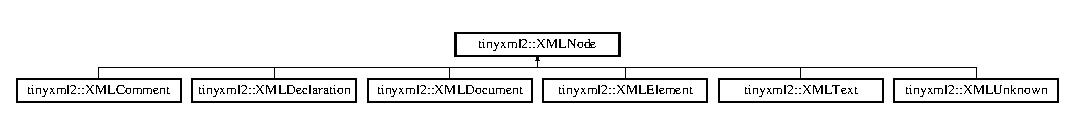
\includegraphics[height=1.145194cm]{classtinyxml2_1_1_x_m_l_node}
\end{center}
\end{figure}
\subsection*{Public Member Functions}
\begin{DoxyCompactItemize}
\item 
const \hyperlink{classtinyxml2_1_1_x_m_l_document}{X\+M\+L\+Document} $\ast$ \hyperlink{classtinyxml2_1_1_x_m_l_node_a2de84cfa4ec3fe249bad745069d145f1}{Get\+Document} () const
\begin{DoxyCompactList}\small\item\em Get the \hyperlink{classtinyxml2_1_1_x_m_l_document}{X\+M\+L\+Document} that owns this \hyperlink{classtinyxml2_1_1_x_m_l_node}{X\+M\+L\+Node}. \end{DoxyCompactList}\item 
\hyperlink{classtinyxml2_1_1_x_m_l_document}{X\+M\+L\+Document} $\ast$ \hyperlink{classtinyxml2_1_1_x_m_l_node_af343d1ef0b45c0020e62d784d7e67a68}{Get\+Document} ()
\begin{DoxyCompactList}\small\item\em Get the \hyperlink{classtinyxml2_1_1_x_m_l_document}{X\+M\+L\+Document} that owns this \hyperlink{classtinyxml2_1_1_x_m_l_node}{X\+M\+L\+Node}. \end{DoxyCompactList}\item 
virtual \hyperlink{classtinyxml2_1_1_x_m_l_element}{X\+M\+L\+Element} $\ast$ \hyperlink{classtinyxml2_1_1_x_m_l_node_aab516e699567f75cc9ab2ef2eee501e8}{To\+Element} ()
\begin{DoxyCompactList}\small\item\em Safely cast to an Element, or null. \end{DoxyCompactList}\item 
virtual \hyperlink{classtinyxml2_1_1_x_m_l_text}{X\+M\+L\+Text} $\ast$ \hyperlink{classtinyxml2_1_1_x_m_l_node_a41c55dab9162d1eb62db2008430e376b}{To\+Text} ()
\begin{DoxyCompactList}\small\item\em Safely cast to Text, or null. \end{DoxyCompactList}\item 
virtual \hyperlink{classtinyxml2_1_1_x_m_l_comment}{X\+M\+L\+Comment} $\ast$ \hyperlink{classtinyxml2_1_1_x_m_l_node_aff47671055aa99840a1c1ebd661e63e3}{To\+Comment} ()
\begin{DoxyCompactList}\small\item\em Safely cast to a Comment, or null. \end{DoxyCompactList}\item 
virtual \hyperlink{classtinyxml2_1_1_x_m_l_document}{X\+M\+L\+Document} $\ast$ \hyperlink{classtinyxml2_1_1_x_m_l_node_a836e2966ed736fc3c94f70e12a2a3357}{To\+Document} ()
\begin{DoxyCompactList}\small\item\em Safely cast to a Document, or null. \end{DoxyCompactList}\item 
virtual \hyperlink{classtinyxml2_1_1_x_m_l_declaration}{X\+M\+L\+Declaration} $\ast$ \hyperlink{classtinyxml2_1_1_x_m_l_node_a174fd4c22c010b58138c1b84a0dfbd51}{To\+Declaration} ()
\begin{DoxyCompactList}\small\item\em Safely cast to a Declaration, or null. \end{DoxyCompactList}\item 
virtual \hyperlink{classtinyxml2_1_1_x_m_l_unknown}{X\+M\+L\+Unknown} $\ast$ \hyperlink{classtinyxml2_1_1_x_m_l_node_a8675a74aa0ada6eccab0c77ef3e5b9bd}{To\+Unknown} ()
\begin{DoxyCompactList}\small\item\em Safely cast to an Unknown, or null. \end{DoxyCompactList}\item 
virtual const \hyperlink{classtinyxml2_1_1_x_m_l_element}{X\+M\+L\+Element} $\ast$ \hyperlink{classtinyxml2_1_1_x_m_l_node_a2c5c843b8f37306f15994ebe882b9346}{To\+Element} () const
\item 
virtual const \hyperlink{classtinyxml2_1_1_x_m_l_text}{X\+M\+L\+Text} $\ast$ \hyperlink{classtinyxml2_1_1_x_m_l_node_acb9ccc1beda27c0efcb0545683c3e7f4}{To\+Text} () const
\item 
virtual const \hyperlink{classtinyxml2_1_1_x_m_l_comment}{X\+M\+L\+Comment} $\ast$ \hyperlink{classtinyxml2_1_1_x_m_l_node_a6a53bb83faf5c0ccc95b6cf74dba0025}{To\+Comment} () const
\item 
virtual const \hyperlink{classtinyxml2_1_1_x_m_l_document}{X\+M\+L\+Document} $\ast$ \hyperlink{classtinyxml2_1_1_x_m_l_node_ae8a5250331a5f12e10843fcb5ef3ef0b}{To\+Document} () const
\item 
virtual const \hyperlink{classtinyxml2_1_1_x_m_l_declaration}{X\+M\+L\+Declaration} $\ast$ \hyperlink{classtinyxml2_1_1_x_m_l_node_ac48bb4bf9eb7bb3654ad4b94945db9a1}{To\+Declaration} () const
\item 
virtual const \hyperlink{classtinyxml2_1_1_x_m_l_unknown}{X\+M\+L\+Unknown} $\ast$ \hyperlink{classtinyxml2_1_1_x_m_l_node_af29ffd6cbe609b6fa04a705256150408}{To\+Unknown} () const
\item 
const char $\ast$ \hyperlink{classtinyxml2_1_1_x_m_l_node_a0485e51c670e741884cfd8362274d680}{Value} () const
\item 
void \hyperlink{classtinyxml2_1_1_x_m_l_node_a09dd68cf9eae137579f6e50f36487513}{Set\+Value} (const char $\ast$val, bool static\+Mem=false)
\item 
int \hyperlink{classtinyxml2_1_1_x_m_l_node_a9b5fc636646fda761d342c72e91cb286}{Get\+Line\+Num} () const
\begin{DoxyCompactList}\small\item\em Gets the line number the node is in, if the document was parsed from a file. \end{DoxyCompactList}\item 
const \hyperlink{classtinyxml2_1_1_x_m_l_node}{X\+M\+L\+Node} $\ast$ \hyperlink{classtinyxml2_1_1_x_m_l_node_ae0f62bc186c56c2e0483ebd52dbfbe34}{Parent} () const
\begin{DoxyCompactList}\small\item\em Get the parent of this node on the D\+OM. \end{DoxyCompactList}\item 
\hyperlink{classtinyxml2_1_1_x_m_l_node}{X\+M\+L\+Node} $\ast$ \hyperlink{classtinyxml2_1_1_x_m_l_node_a76029693a5a54fbb721a41d7a0ca8a97}{Parent} ()
\item 
bool \hyperlink{classtinyxml2_1_1_x_m_l_node_ac3ab489e6e202a3cd1762d3b332e89d4}{No\+Children} () const
\begin{DoxyCompactList}\small\item\em Returns true if this node has no children. \end{DoxyCompactList}\item 
const \hyperlink{classtinyxml2_1_1_x_m_l_node}{X\+M\+L\+Node} $\ast$ \hyperlink{classtinyxml2_1_1_x_m_l_node_ae7dc225e1018cdd685f7563593a1fe08}{First\+Child} () const
\begin{DoxyCompactList}\small\item\em Get the first child node, or null if none exists. \end{DoxyCompactList}\item 
\hyperlink{classtinyxml2_1_1_x_m_l_node}{X\+M\+L\+Node} $\ast$ \hyperlink{classtinyxml2_1_1_x_m_l_node_a2d6c70c475146b48bc93a7fafdeff5e0}{First\+Child} ()
\item 
const \hyperlink{classtinyxml2_1_1_x_m_l_element}{X\+M\+L\+Element} $\ast$ \hyperlink{classtinyxml2_1_1_x_m_l_node_a1bec132dcf085284e0a10755f2cf0d57}{First\+Child\+Element} (const char $\ast$name=0) const
\item 
\hyperlink{classtinyxml2_1_1_x_m_l_element}{X\+M\+L\+Element} $\ast$ \hyperlink{classtinyxml2_1_1_x_m_l_node_af1e0e475cc27d5e7eeaf4d732691b741}{First\+Child\+Element} (const char $\ast$name=0)
\item 
const \hyperlink{classtinyxml2_1_1_x_m_l_node}{X\+M\+L\+Node} $\ast$ \hyperlink{classtinyxml2_1_1_x_m_l_node_a9b8583a277e8e26f4cbbb5492786778e}{Last\+Child} () const
\begin{DoxyCompactList}\small\item\em Get the last child node, or null if none exists. \end{DoxyCompactList}\item 
\hyperlink{classtinyxml2_1_1_x_m_l_node}{X\+M\+L\+Node} $\ast$ \hyperlink{classtinyxml2_1_1_x_m_l_node_ad7552c8cb1dc0cb6f3bdc14a9d115dbf}{Last\+Child} ()
\item 
const \hyperlink{classtinyxml2_1_1_x_m_l_element}{X\+M\+L\+Element} $\ast$ \hyperlink{classtinyxml2_1_1_x_m_l_node_a609e02f02044f39b928d1a3e0de9f532}{Last\+Child\+Element} (const char $\ast$name=0) const
\item 
\hyperlink{classtinyxml2_1_1_x_m_l_element}{X\+M\+L\+Element} $\ast$ \hyperlink{classtinyxml2_1_1_x_m_l_node_a1b77a8194d059665a4412ebfea276878}{Last\+Child\+Element} (const char $\ast$name=0)
\item 
const \hyperlink{classtinyxml2_1_1_x_m_l_node}{X\+M\+L\+Node} $\ast$ \hyperlink{classtinyxml2_1_1_x_m_l_node_aac667c513d445f8b783e1e15ef9d3551}{Previous\+Sibling} () const
\begin{DoxyCompactList}\small\item\em Get the previous (left) sibling node of this node. \end{DoxyCompactList}\item 
\hyperlink{classtinyxml2_1_1_x_m_l_node}{X\+M\+L\+Node} $\ast$ \hyperlink{classtinyxml2_1_1_x_m_l_node_ae760e5e7e766df1d2cf3bb4a847876d6}{Previous\+Sibling} ()
\item 
const \hyperlink{classtinyxml2_1_1_x_m_l_element}{X\+M\+L\+Element} $\ast$ \hyperlink{classtinyxml2_1_1_x_m_l_node_a9453cda5e970375a7b1b2099f8a7c40a}{Previous\+Sibling\+Element} (const char $\ast$name=0) const
\begin{DoxyCompactList}\small\item\em Get the previous (left) sibling element of this node, with an optionally supplied name. \end{DoxyCompactList}\item 
\hyperlink{classtinyxml2_1_1_x_m_l_element}{X\+M\+L\+Element} $\ast$ \hyperlink{classtinyxml2_1_1_x_m_l_node_ae4f37eb6cd405bdf1d57caa066e36d87}{Previous\+Sibling\+Element} (const char $\ast$name=0)
\item 
const \hyperlink{classtinyxml2_1_1_x_m_l_node}{X\+M\+L\+Node} $\ast$ \hyperlink{classtinyxml2_1_1_x_m_l_node_a79db9ef0fe014d27790f2218b87bcbb5}{Next\+Sibling} () const
\begin{DoxyCompactList}\small\item\em Get the next (right) sibling node of this node. \end{DoxyCompactList}\item 
\hyperlink{classtinyxml2_1_1_x_m_l_node}{X\+M\+L\+Node} $\ast$ \hyperlink{classtinyxml2_1_1_x_m_l_node_aeb7d4dfd8fb924ef86e7cb72183acbac}{Next\+Sibling} ()
\item 
const \hyperlink{classtinyxml2_1_1_x_m_l_element}{X\+M\+L\+Element} $\ast$ \hyperlink{classtinyxml2_1_1_x_m_l_node_a14ea560df31110ff07a9f566171bf797}{Next\+Sibling\+Element} (const char $\ast$name=0) const
\begin{DoxyCompactList}\small\item\em Get the next (right) sibling element of this node, with an optionally supplied name. \end{DoxyCompactList}\item 
\hyperlink{classtinyxml2_1_1_x_m_l_element}{X\+M\+L\+Element} $\ast$ \hyperlink{classtinyxml2_1_1_x_m_l_node_af1225412584d4a2126f55e96a12e0ec0}{Next\+Sibling\+Element} (const char $\ast$name=0)
\item 
\hyperlink{classtinyxml2_1_1_x_m_l_node}{X\+M\+L\+Node} $\ast$ \hyperlink{classtinyxml2_1_1_x_m_l_node_ae3b422e98914d6002ca99bb1d2837103}{Insert\+End\+Child} (\hyperlink{classtinyxml2_1_1_x_m_l_node}{X\+M\+L\+Node} $\ast$add\+This)
\item 
\hyperlink{classtinyxml2_1_1_x_m_l_node}{X\+M\+L\+Node} $\ast$ \hyperlink{classtinyxml2_1_1_x_m_l_node_a663e3a5a378169fd477378f4d17a7649}{Link\+End\+Child} (\hyperlink{classtinyxml2_1_1_x_m_l_node}{X\+M\+L\+Node} $\ast$add\+This)
\item 
\hyperlink{classtinyxml2_1_1_x_m_l_node}{X\+M\+L\+Node} $\ast$ \hyperlink{classtinyxml2_1_1_x_m_l_node_ac609a8f3ea949027f439280c640bbaf2}{Insert\+First\+Child} (\hyperlink{classtinyxml2_1_1_x_m_l_node}{X\+M\+L\+Node} $\ast$add\+This)
\item 
\hyperlink{classtinyxml2_1_1_x_m_l_node}{X\+M\+L\+Node} $\ast$ \hyperlink{classtinyxml2_1_1_x_m_l_node_a9275138a1b8dd5d8e2c26789bdc23ac8}{Insert\+After\+Child} (\hyperlink{classtinyxml2_1_1_x_m_l_node}{X\+M\+L\+Node} $\ast$after\+This, \hyperlink{classtinyxml2_1_1_x_m_l_node}{X\+M\+L\+Node} $\ast$add\+This)
\item 
void \hyperlink{classtinyxml2_1_1_x_m_l_node_a0360085cc54df5bff85d5c5da13afdce}{Delete\+Children} ()
\item 
void \hyperlink{classtinyxml2_1_1_x_m_l_node_a363b6edbd6ebd55f8387d2b89f2b0921}{Delete\+Child} (\hyperlink{classtinyxml2_1_1_x_m_l_node}{X\+M\+L\+Node} $\ast$node)
\item 
virtual \hyperlink{classtinyxml2_1_1_x_m_l_node}{X\+M\+L\+Node} $\ast$ \hyperlink{classtinyxml2_1_1_x_m_l_node_a8402cbd3129d20e9e6024bbcc0531283}{Shallow\+Clone} (\hyperlink{classtinyxml2_1_1_x_m_l_document}{X\+M\+L\+Document} $\ast$document) const =0
\item 
virtual bool \hyperlink{classtinyxml2_1_1_x_m_l_node_a7ce18b751c3ea09eac292dca264f9226}{Shallow\+Equal} (const \hyperlink{classtinyxml2_1_1_x_m_l_node}{X\+M\+L\+Node} $\ast$compare) const =0
\item 
virtual bool \hyperlink{classtinyxml2_1_1_x_m_l_node_a81e66df0a44c67a7af17f3b77a152785}{Accept} (\hyperlink{classtinyxml2_1_1_x_m_l_visitor}{X\+M\+L\+Visitor} $\ast$visitor) const =0
\item 
void \hyperlink{classtinyxml2_1_1_x_m_l_node_a002978fc889cc011d143185f2377eca2}{Set\+User\+Data} (void $\ast$user\+Data)
\item 
void $\ast$ \hyperlink{classtinyxml2_1_1_x_m_l_node_a7f0687574afa03bc479dc44f29db0afe}{Get\+User\+Data} () const
\end{DoxyCompactItemize}
\subsection*{Protected Member Functions}
\begin{DoxyCompactItemize}
\item 
\hyperlink{classtinyxml2_1_1_x_m_l_node_a29868df6ca383d574f584dfdd15105b6}{X\+M\+L\+Node} (\hyperlink{classtinyxml2_1_1_x_m_l_document}{X\+M\+L\+Document} $\ast$)
\item 
virtual \hyperlink{classtinyxml2_1_1_x_m_l_node_a8f41e898cdd4da4cdbb7f05b0c7d9f69}{$\sim$\+X\+M\+L\+Node} ()
\item 
virtual char $\ast$ \hyperlink{classtinyxml2_1_1_x_m_l_node_a0afc27892998f31735f6225edb40a40d}{Parse\+Deep} (char $\ast$, \hyperlink{classtinyxml2_1_1_str_pair}{Str\+Pair} $\ast$, int $\ast$)
\end{DoxyCompactItemize}
\subsection*{Protected Attributes}
\begin{DoxyCompactItemize}
\item 
\hyperlink{classtinyxml2_1_1_x_m_l_document}{X\+M\+L\+Document} $\ast$ \hyperlink{classtinyxml2_1_1_x_m_l_node_a8d2d2be0bb6797625551eb0e91f0ff62}{\+\_\+document}
\item 
\hyperlink{classtinyxml2_1_1_x_m_l_node}{X\+M\+L\+Node} $\ast$ \hyperlink{classtinyxml2_1_1_x_m_l_node_a176dd1c4965c21c366de192164aa2c13}{\+\_\+parent}
\item 
\hyperlink{classtinyxml2_1_1_str_pair}{Str\+Pair} \hyperlink{classtinyxml2_1_1_x_m_l_node_a3ea9884098b8379de2bb5ab3fc85c0fc}{\+\_\+value}
\item 
int \hyperlink{classtinyxml2_1_1_x_m_l_node_ab336ed023e15be202ff3b410be01b804}{\+\_\+parse\+Line\+Num}
\item 
\hyperlink{classtinyxml2_1_1_x_m_l_node}{X\+M\+L\+Node} $\ast$ \hyperlink{classtinyxml2_1_1_x_m_l_node_aa20c91e4213dc930c5bdf420322ca342}{\+\_\+first\+Child}
\item 
\hyperlink{classtinyxml2_1_1_x_m_l_node}{X\+M\+L\+Node} $\ast$ \hyperlink{classtinyxml2_1_1_x_m_l_node_a099b6560ae44ab9edb8453aaf1a3747b}{\+\_\+last\+Child}
\item 
\hyperlink{classtinyxml2_1_1_x_m_l_node}{X\+M\+L\+Node} $\ast$ \hyperlink{classtinyxml2_1_1_x_m_l_node_a9739eb0fb9a1188266052055e7a6bf6b}{\+\_\+prev}
\item 
\hyperlink{classtinyxml2_1_1_x_m_l_node}{X\+M\+L\+Node} $\ast$ \hyperlink{classtinyxml2_1_1_x_m_l_node_a27e985496b37dd00eb5b9cf59b9e3fb1}{\+\_\+next}
\item 
void $\ast$ \hyperlink{classtinyxml2_1_1_x_m_l_node_ac2d5cc463a6c95ec5907d57a119c56da}{\+\_\+user\+Data}
\end{DoxyCompactItemize}
\subsection*{Friends}
\begin{DoxyCompactItemize}
\item 
class \hyperlink{classtinyxml2_1_1_x_m_l_node_a4eee3bda60c60a30e4e8cd4ea91c4c6e}{X\+M\+L\+Document}
\item 
class \hyperlink{classtinyxml2_1_1_x_m_l_node_ac2fba9b6e452829dd892f7392c24e0eb}{X\+M\+L\+Element}
\end{DoxyCompactItemize}


\subsection{Detailed Description}
\hyperlink{classtinyxml2_1_1_x_m_l_node}{X\+M\+L\+Node} is a base class for every object that is in the X\+ML Document Object Model (D\+OM), except X\+M\+L\+Attributes. Nodes have siblings, a parent, and children which can be navigated. A node is always in a \hyperlink{classtinyxml2_1_1_x_m_l_document}{X\+M\+L\+Document}. The type of a \hyperlink{classtinyxml2_1_1_x_m_l_node}{X\+M\+L\+Node} can be queried, and it can be cast to its more defined type.

A \hyperlink{classtinyxml2_1_1_x_m_l_document}{X\+M\+L\+Document} allocates memory for all its Nodes. When the \hyperlink{classtinyxml2_1_1_x_m_l_document}{X\+M\+L\+Document} gets deleted, all its Nodes will also be deleted.

\begin{DoxyVerb}A Document can contain: Element (container or leaf)
Comment (leaf)
Unknown (leaf)
Declaration( leaf )

An Element can contain: Element (container or leaf)
Text    (leaf)
Attributes (not on tree)
Comment (leaf)
Unknown (leaf)\end{DoxyVerb}
 

\subsection{Constructor \& Destructor Documentation}
\mbox{\Hypertarget{classtinyxml2_1_1_x_m_l_node_a29868df6ca383d574f584dfdd15105b6}\label{classtinyxml2_1_1_x_m_l_node_a29868df6ca383d574f584dfdd15105b6}} 
\index{tinyxml2\+::\+X\+M\+L\+Node@{tinyxml2\+::\+X\+M\+L\+Node}!X\+M\+L\+Node@{X\+M\+L\+Node}}
\index{X\+M\+L\+Node@{X\+M\+L\+Node}!tinyxml2\+::\+X\+M\+L\+Node@{tinyxml2\+::\+X\+M\+L\+Node}}
\subsubsection{\texorpdfstring{X\+M\+L\+Node()}{XMLNode()}}
{\footnotesize\ttfamily tinyxml2\+::\+X\+M\+L\+Node\+::\+X\+M\+L\+Node (\begin{DoxyParamCaption}\item[{\hyperlink{classtinyxml2_1_1_x_m_l_document}{X\+M\+L\+Document} $\ast$}]{doc }\end{DoxyParamCaption})\hspace{0.3cm}{\ttfamily [protected]}}

\mbox{\Hypertarget{classtinyxml2_1_1_x_m_l_node_a8f41e898cdd4da4cdbb7f05b0c7d9f69}\label{classtinyxml2_1_1_x_m_l_node_a8f41e898cdd4da4cdbb7f05b0c7d9f69}} 
\index{tinyxml2\+::\+X\+M\+L\+Node@{tinyxml2\+::\+X\+M\+L\+Node}!````~X\+M\+L\+Node@{$\sim$\+X\+M\+L\+Node}}
\index{````~X\+M\+L\+Node@{$\sim$\+X\+M\+L\+Node}!tinyxml2\+::\+X\+M\+L\+Node@{tinyxml2\+::\+X\+M\+L\+Node}}
\subsubsection{\texorpdfstring{$\sim$\+X\+M\+L\+Node()}{~XMLNode()}}
{\footnotesize\ttfamily tinyxml2\+::\+X\+M\+L\+Node\+::$\sim$\+X\+M\+L\+Node (\begin{DoxyParamCaption}{ }\end{DoxyParamCaption})\hspace{0.3cm}{\ttfamily [protected]}, {\ttfamily [virtual]}}



\subsection{Member Function Documentation}
\mbox{\Hypertarget{classtinyxml2_1_1_x_m_l_node_a81e66df0a44c67a7af17f3b77a152785}\label{classtinyxml2_1_1_x_m_l_node_a81e66df0a44c67a7af17f3b77a152785}} 
\index{tinyxml2\+::\+X\+M\+L\+Node@{tinyxml2\+::\+X\+M\+L\+Node}!Accept@{Accept}}
\index{Accept@{Accept}!tinyxml2\+::\+X\+M\+L\+Node@{tinyxml2\+::\+X\+M\+L\+Node}}
\subsubsection{\texorpdfstring{Accept()}{Accept()}}
{\footnotesize\ttfamily virtual bool tinyxml2\+::\+X\+M\+L\+Node\+::\+Accept (\begin{DoxyParamCaption}\item[{\hyperlink{classtinyxml2_1_1_x_m_l_visitor}{X\+M\+L\+Visitor} $\ast$}]{visitor }\end{DoxyParamCaption}) const\hspace{0.3cm}{\ttfamily [pure virtual]}}

Accept a hierarchical visit of the nodes in the Tiny\+X\+M\+L-\/2 D\+OM. Every node in the X\+ML tree will be conditionally visited and the host will be called back via the \hyperlink{classtinyxml2_1_1_x_m_l_visitor}{X\+M\+L\+Visitor} interface.

This is essentially a S\+AX interface for Tiny\+X\+M\+L-\/2. (Note however it doesn\textquotesingle{}t re-\/parse the X\+ML for the callbacks, so the performance of Tiny\+X\+M\+L-\/2 is unchanged by using this interface versus any other.)

The interface has been based on ideas from\+:


\begin{DoxyItemize}
\item \href{http://www.saxproject.org/}{\tt http\+://www.\+saxproject.\+org/}
\item \href{http://c2.com/cgi/wiki?HierarchicalVisitorPattern}{\tt http\+://c2.\+com/cgi/wiki?\+Hierarchical\+Visitor\+Pattern}
\end{DoxyItemize}

Which are both good references for \char`\"{}visiting\char`\"{}.

An example of using \hyperlink{classtinyxml2_1_1_x_m_l_node_a81e66df0a44c67a7af17f3b77a152785}{Accept()}\+: \begin{DoxyVerb}XMLPrinter printer;
tinyxmlDoc.Accept( &printer );
const char* xmlcstr = printer.CStr();
\end{DoxyVerb}
 

Implemented in \hyperlink{classtinyxml2_1_1_x_m_l_document_ab7be651917a35ab1ff0e4e6d4e565cdf}{tinyxml2\+::\+X\+M\+L\+Document}, \hyperlink{classtinyxml2_1_1_x_m_l_element_a9b2119831e8b85827d5d3e5076788e4a}{tinyxml2\+::\+X\+M\+L\+Element}, \hyperlink{classtinyxml2_1_1_x_m_l_unknown_a8a06b8c82117ca969a432e17a46830fc}{tinyxml2\+::\+X\+M\+L\+Unknown}, \hyperlink{classtinyxml2_1_1_x_m_l_declaration_acf47629d9fc08ed6f1c164a97bcf794b}{tinyxml2\+::\+X\+M\+L\+Declaration}, \hyperlink{classtinyxml2_1_1_x_m_l_comment_a27b37d16cea01b5329dfbbb4f9508e39}{tinyxml2\+::\+X\+M\+L\+Comment}, and \hyperlink{classtinyxml2_1_1_x_m_l_text_a537c60d7e18fb59c45ac2737a29ac47a}{tinyxml2\+::\+X\+M\+L\+Text}.

\mbox{\Hypertarget{classtinyxml2_1_1_x_m_l_node_a363b6edbd6ebd55f8387d2b89f2b0921}\label{classtinyxml2_1_1_x_m_l_node_a363b6edbd6ebd55f8387d2b89f2b0921}} 
\index{tinyxml2\+::\+X\+M\+L\+Node@{tinyxml2\+::\+X\+M\+L\+Node}!Delete\+Child@{Delete\+Child}}
\index{Delete\+Child@{Delete\+Child}!tinyxml2\+::\+X\+M\+L\+Node@{tinyxml2\+::\+X\+M\+L\+Node}}
\subsubsection{\texorpdfstring{Delete\+Child()}{DeleteChild()}}
{\footnotesize\ttfamily void tinyxml2\+::\+X\+M\+L\+Node\+::\+Delete\+Child (\begin{DoxyParamCaption}\item[{\hyperlink{classtinyxml2_1_1_x_m_l_node}{X\+M\+L\+Node} $\ast$}]{node }\end{DoxyParamCaption})}

Delete a child of this node. \mbox{\Hypertarget{classtinyxml2_1_1_x_m_l_node_a0360085cc54df5bff85d5c5da13afdce}\label{classtinyxml2_1_1_x_m_l_node_a0360085cc54df5bff85d5c5da13afdce}} 
\index{tinyxml2\+::\+X\+M\+L\+Node@{tinyxml2\+::\+X\+M\+L\+Node}!Delete\+Children@{Delete\+Children}}
\index{Delete\+Children@{Delete\+Children}!tinyxml2\+::\+X\+M\+L\+Node@{tinyxml2\+::\+X\+M\+L\+Node}}
\subsubsection{\texorpdfstring{Delete\+Children()}{DeleteChildren()}}
{\footnotesize\ttfamily void tinyxml2\+::\+X\+M\+L\+Node\+::\+Delete\+Children (\begin{DoxyParamCaption}{ }\end{DoxyParamCaption})}

Delete all the children of this node. \mbox{\Hypertarget{classtinyxml2_1_1_x_m_l_node_ae7dc225e1018cdd685f7563593a1fe08}\label{classtinyxml2_1_1_x_m_l_node_ae7dc225e1018cdd685f7563593a1fe08}} 
\index{tinyxml2\+::\+X\+M\+L\+Node@{tinyxml2\+::\+X\+M\+L\+Node}!First\+Child@{First\+Child}}
\index{First\+Child@{First\+Child}!tinyxml2\+::\+X\+M\+L\+Node@{tinyxml2\+::\+X\+M\+L\+Node}}
\subsubsection{\texorpdfstring{First\+Child()}{FirstChild()}\hspace{0.1cm}{\footnotesize\ttfamily [1/2]}}
{\footnotesize\ttfamily const \hyperlink{classtinyxml2_1_1_x_m_l_node}{X\+M\+L\+Node}$\ast$ tinyxml2\+::\+X\+M\+L\+Node\+::\+First\+Child (\begin{DoxyParamCaption}{ }\end{DoxyParamCaption}) const\hspace{0.3cm}{\ttfamily [inline]}}



Get the first child node, or null if none exists. 

\mbox{\Hypertarget{classtinyxml2_1_1_x_m_l_node_a2d6c70c475146b48bc93a7fafdeff5e0}\label{classtinyxml2_1_1_x_m_l_node_a2d6c70c475146b48bc93a7fafdeff5e0}} 
\index{tinyxml2\+::\+X\+M\+L\+Node@{tinyxml2\+::\+X\+M\+L\+Node}!First\+Child@{First\+Child}}
\index{First\+Child@{First\+Child}!tinyxml2\+::\+X\+M\+L\+Node@{tinyxml2\+::\+X\+M\+L\+Node}}
\subsubsection{\texorpdfstring{First\+Child()}{FirstChild()}\hspace{0.1cm}{\footnotesize\ttfamily [2/2]}}
{\footnotesize\ttfamily \hyperlink{classtinyxml2_1_1_x_m_l_node}{X\+M\+L\+Node}$\ast$ tinyxml2\+::\+X\+M\+L\+Node\+::\+First\+Child (\begin{DoxyParamCaption}{ }\end{DoxyParamCaption})\hspace{0.3cm}{\ttfamily [inline]}}

\mbox{\Hypertarget{classtinyxml2_1_1_x_m_l_node_a1bec132dcf085284e0a10755f2cf0d57}\label{classtinyxml2_1_1_x_m_l_node_a1bec132dcf085284e0a10755f2cf0d57}} 
\index{tinyxml2\+::\+X\+M\+L\+Node@{tinyxml2\+::\+X\+M\+L\+Node}!First\+Child\+Element@{First\+Child\+Element}}
\index{First\+Child\+Element@{First\+Child\+Element}!tinyxml2\+::\+X\+M\+L\+Node@{tinyxml2\+::\+X\+M\+L\+Node}}
\subsubsection{\texorpdfstring{First\+Child\+Element()}{FirstChildElement()}\hspace{0.1cm}{\footnotesize\ttfamily [1/2]}}
{\footnotesize\ttfamily const \hyperlink{classtinyxml2_1_1_x_m_l_element}{X\+M\+L\+Element} $\ast$ tinyxml2\+::\+X\+M\+L\+Node\+::\+First\+Child\+Element (\begin{DoxyParamCaption}\item[{const char $\ast$}]{name = {\ttfamily 0} }\end{DoxyParamCaption}) const}

Get the first child element, or optionally the first child element with the specified name. \mbox{\Hypertarget{classtinyxml2_1_1_x_m_l_node_af1e0e475cc27d5e7eeaf4d732691b741}\label{classtinyxml2_1_1_x_m_l_node_af1e0e475cc27d5e7eeaf4d732691b741}} 
\index{tinyxml2\+::\+X\+M\+L\+Node@{tinyxml2\+::\+X\+M\+L\+Node}!First\+Child\+Element@{First\+Child\+Element}}
\index{First\+Child\+Element@{First\+Child\+Element}!tinyxml2\+::\+X\+M\+L\+Node@{tinyxml2\+::\+X\+M\+L\+Node}}
\subsubsection{\texorpdfstring{First\+Child\+Element()}{FirstChildElement()}\hspace{0.1cm}{\footnotesize\ttfamily [2/2]}}
{\footnotesize\ttfamily \hyperlink{classtinyxml2_1_1_x_m_l_element}{X\+M\+L\+Element}$\ast$ tinyxml2\+::\+X\+M\+L\+Node\+::\+First\+Child\+Element (\begin{DoxyParamCaption}\item[{const char $\ast$}]{name = {\ttfamily 0} }\end{DoxyParamCaption})\hspace{0.3cm}{\ttfamily [inline]}}

\mbox{\Hypertarget{classtinyxml2_1_1_x_m_l_node_a2de84cfa4ec3fe249bad745069d145f1}\label{classtinyxml2_1_1_x_m_l_node_a2de84cfa4ec3fe249bad745069d145f1}} 
\index{tinyxml2\+::\+X\+M\+L\+Node@{tinyxml2\+::\+X\+M\+L\+Node}!Get\+Document@{Get\+Document}}
\index{Get\+Document@{Get\+Document}!tinyxml2\+::\+X\+M\+L\+Node@{tinyxml2\+::\+X\+M\+L\+Node}}
\subsubsection{\texorpdfstring{Get\+Document()}{GetDocument()}\hspace{0.1cm}{\footnotesize\ttfamily [1/2]}}
{\footnotesize\ttfamily const \hyperlink{classtinyxml2_1_1_x_m_l_document}{X\+M\+L\+Document}$\ast$ tinyxml2\+::\+X\+M\+L\+Node\+::\+Get\+Document (\begin{DoxyParamCaption}{ }\end{DoxyParamCaption}) const\hspace{0.3cm}{\ttfamily [inline]}}



Get the \hyperlink{classtinyxml2_1_1_x_m_l_document}{X\+M\+L\+Document} that owns this \hyperlink{classtinyxml2_1_1_x_m_l_node}{X\+M\+L\+Node}. 

\mbox{\Hypertarget{classtinyxml2_1_1_x_m_l_node_af343d1ef0b45c0020e62d784d7e67a68}\label{classtinyxml2_1_1_x_m_l_node_af343d1ef0b45c0020e62d784d7e67a68}} 
\index{tinyxml2\+::\+X\+M\+L\+Node@{tinyxml2\+::\+X\+M\+L\+Node}!Get\+Document@{Get\+Document}}
\index{Get\+Document@{Get\+Document}!tinyxml2\+::\+X\+M\+L\+Node@{tinyxml2\+::\+X\+M\+L\+Node}}
\subsubsection{\texorpdfstring{Get\+Document()}{GetDocument()}\hspace{0.1cm}{\footnotesize\ttfamily [2/2]}}
{\footnotesize\ttfamily \hyperlink{classtinyxml2_1_1_x_m_l_document}{X\+M\+L\+Document}$\ast$ tinyxml2\+::\+X\+M\+L\+Node\+::\+Get\+Document (\begin{DoxyParamCaption}{ }\end{DoxyParamCaption})\hspace{0.3cm}{\ttfamily [inline]}}



Get the \hyperlink{classtinyxml2_1_1_x_m_l_document}{X\+M\+L\+Document} that owns this \hyperlink{classtinyxml2_1_1_x_m_l_node}{X\+M\+L\+Node}. 

\mbox{\Hypertarget{classtinyxml2_1_1_x_m_l_node_a9b5fc636646fda761d342c72e91cb286}\label{classtinyxml2_1_1_x_m_l_node_a9b5fc636646fda761d342c72e91cb286}} 
\index{tinyxml2\+::\+X\+M\+L\+Node@{tinyxml2\+::\+X\+M\+L\+Node}!Get\+Line\+Num@{Get\+Line\+Num}}
\index{Get\+Line\+Num@{Get\+Line\+Num}!tinyxml2\+::\+X\+M\+L\+Node@{tinyxml2\+::\+X\+M\+L\+Node}}
\subsubsection{\texorpdfstring{Get\+Line\+Num()}{GetLineNum()}}
{\footnotesize\ttfamily int tinyxml2\+::\+X\+M\+L\+Node\+::\+Get\+Line\+Num (\begin{DoxyParamCaption}{ }\end{DoxyParamCaption}) const\hspace{0.3cm}{\ttfamily [inline]}}



Gets the line number the node is in, if the document was parsed from a file. 

\mbox{\Hypertarget{classtinyxml2_1_1_x_m_l_node_a7f0687574afa03bc479dc44f29db0afe}\label{classtinyxml2_1_1_x_m_l_node_a7f0687574afa03bc479dc44f29db0afe}} 
\index{tinyxml2\+::\+X\+M\+L\+Node@{tinyxml2\+::\+X\+M\+L\+Node}!Get\+User\+Data@{Get\+User\+Data}}
\index{Get\+User\+Data@{Get\+User\+Data}!tinyxml2\+::\+X\+M\+L\+Node@{tinyxml2\+::\+X\+M\+L\+Node}}
\subsubsection{\texorpdfstring{Get\+User\+Data()}{GetUserData()}}
{\footnotesize\ttfamily void$\ast$ tinyxml2\+::\+X\+M\+L\+Node\+::\+Get\+User\+Data (\begin{DoxyParamCaption}{ }\end{DoxyParamCaption}) const\hspace{0.3cm}{\ttfamily [inline]}}

Get user data set into the \hyperlink{classtinyxml2_1_1_x_m_l_node}{X\+M\+L\+Node}. Tiny\+X\+M\+L-\/2 in no way processes or interprets user data. It is initially 0. \mbox{\Hypertarget{classtinyxml2_1_1_x_m_l_node_a9275138a1b8dd5d8e2c26789bdc23ac8}\label{classtinyxml2_1_1_x_m_l_node_a9275138a1b8dd5d8e2c26789bdc23ac8}} 
\index{tinyxml2\+::\+X\+M\+L\+Node@{tinyxml2\+::\+X\+M\+L\+Node}!Insert\+After\+Child@{Insert\+After\+Child}}
\index{Insert\+After\+Child@{Insert\+After\+Child}!tinyxml2\+::\+X\+M\+L\+Node@{tinyxml2\+::\+X\+M\+L\+Node}}
\subsubsection{\texorpdfstring{Insert\+After\+Child()}{InsertAfterChild()}}
{\footnotesize\ttfamily \hyperlink{classtinyxml2_1_1_x_m_l_node}{X\+M\+L\+Node} $\ast$ tinyxml2\+::\+X\+M\+L\+Node\+::\+Insert\+After\+Child (\begin{DoxyParamCaption}\item[{\hyperlink{classtinyxml2_1_1_x_m_l_node}{X\+M\+L\+Node} $\ast$}]{after\+This,  }\item[{\hyperlink{classtinyxml2_1_1_x_m_l_node}{X\+M\+L\+Node} $\ast$}]{add\+This }\end{DoxyParamCaption})}

Add a node after the specified child node. If the child node is already part of the document, it is moved from its old location to the new location. Returns the add\+This argument or 0 if the after\+This node is not a child of this node, or if the node does not belong to the same document. \mbox{\Hypertarget{classtinyxml2_1_1_x_m_l_node_ae3b422e98914d6002ca99bb1d2837103}\label{classtinyxml2_1_1_x_m_l_node_ae3b422e98914d6002ca99bb1d2837103}} 
\index{tinyxml2\+::\+X\+M\+L\+Node@{tinyxml2\+::\+X\+M\+L\+Node}!Insert\+End\+Child@{Insert\+End\+Child}}
\index{Insert\+End\+Child@{Insert\+End\+Child}!tinyxml2\+::\+X\+M\+L\+Node@{tinyxml2\+::\+X\+M\+L\+Node}}
\subsubsection{\texorpdfstring{Insert\+End\+Child()}{InsertEndChild()}}
{\footnotesize\ttfamily \hyperlink{classtinyxml2_1_1_x_m_l_node}{X\+M\+L\+Node} $\ast$ tinyxml2\+::\+X\+M\+L\+Node\+::\+Insert\+End\+Child (\begin{DoxyParamCaption}\item[{\hyperlink{classtinyxml2_1_1_x_m_l_node}{X\+M\+L\+Node} $\ast$}]{add\+This }\end{DoxyParamCaption})}

Add a child node as the last (right) child. If the child node is already part of the document, it is moved from its old location to the new location. Returns the add\+This argument or 0 if the node does not belong to the same document. \mbox{\Hypertarget{classtinyxml2_1_1_x_m_l_node_ac609a8f3ea949027f439280c640bbaf2}\label{classtinyxml2_1_1_x_m_l_node_ac609a8f3ea949027f439280c640bbaf2}} 
\index{tinyxml2\+::\+X\+M\+L\+Node@{tinyxml2\+::\+X\+M\+L\+Node}!Insert\+First\+Child@{Insert\+First\+Child}}
\index{Insert\+First\+Child@{Insert\+First\+Child}!tinyxml2\+::\+X\+M\+L\+Node@{tinyxml2\+::\+X\+M\+L\+Node}}
\subsubsection{\texorpdfstring{Insert\+First\+Child()}{InsertFirstChild()}}
{\footnotesize\ttfamily \hyperlink{classtinyxml2_1_1_x_m_l_node}{X\+M\+L\+Node} $\ast$ tinyxml2\+::\+X\+M\+L\+Node\+::\+Insert\+First\+Child (\begin{DoxyParamCaption}\item[{\hyperlink{classtinyxml2_1_1_x_m_l_node}{X\+M\+L\+Node} $\ast$}]{add\+This }\end{DoxyParamCaption})}

Add a child node as the first (left) child. If the child node is already part of the document, it is moved from its old location to the new location. Returns the add\+This argument or 0 if the node does not belong to the same document. \mbox{\Hypertarget{classtinyxml2_1_1_x_m_l_node_a9b8583a277e8e26f4cbbb5492786778e}\label{classtinyxml2_1_1_x_m_l_node_a9b8583a277e8e26f4cbbb5492786778e}} 
\index{tinyxml2\+::\+X\+M\+L\+Node@{tinyxml2\+::\+X\+M\+L\+Node}!Last\+Child@{Last\+Child}}
\index{Last\+Child@{Last\+Child}!tinyxml2\+::\+X\+M\+L\+Node@{tinyxml2\+::\+X\+M\+L\+Node}}
\subsubsection{\texorpdfstring{Last\+Child()}{LastChild()}\hspace{0.1cm}{\footnotesize\ttfamily [1/2]}}
{\footnotesize\ttfamily const \hyperlink{classtinyxml2_1_1_x_m_l_node}{X\+M\+L\+Node}$\ast$ tinyxml2\+::\+X\+M\+L\+Node\+::\+Last\+Child (\begin{DoxyParamCaption}{ }\end{DoxyParamCaption}) const\hspace{0.3cm}{\ttfamily [inline]}}



Get the last child node, or null if none exists. 

\mbox{\Hypertarget{classtinyxml2_1_1_x_m_l_node_ad7552c8cb1dc0cb6f3bdc14a9d115dbf}\label{classtinyxml2_1_1_x_m_l_node_ad7552c8cb1dc0cb6f3bdc14a9d115dbf}} 
\index{tinyxml2\+::\+X\+M\+L\+Node@{tinyxml2\+::\+X\+M\+L\+Node}!Last\+Child@{Last\+Child}}
\index{Last\+Child@{Last\+Child}!tinyxml2\+::\+X\+M\+L\+Node@{tinyxml2\+::\+X\+M\+L\+Node}}
\subsubsection{\texorpdfstring{Last\+Child()}{LastChild()}\hspace{0.1cm}{\footnotesize\ttfamily [2/2]}}
{\footnotesize\ttfamily \hyperlink{classtinyxml2_1_1_x_m_l_node}{X\+M\+L\+Node}$\ast$ tinyxml2\+::\+X\+M\+L\+Node\+::\+Last\+Child (\begin{DoxyParamCaption}{ }\end{DoxyParamCaption})\hspace{0.3cm}{\ttfamily [inline]}}

\mbox{\Hypertarget{classtinyxml2_1_1_x_m_l_node_a609e02f02044f39b928d1a3e0de9f532}\label{classtinyxml2_1_1_x_m_l_node_a609e02f02044f39b928d1a3e0de9f532}} 
\index{tinyxml2\+::\+X\+M\+L\+Node@{tinyxml2\+::\+X\+M\+L\+Node}!Last\+Child\+Element@{Last\+Child\+Element}}
\index{Last\+Child\+Element@{Last\+Child\+Element}!tinyxml2\+::\+X\+M\+L\+Node@{tinyxml2\+::\+X\+M\+L\+Node}}
\subsubsection{\texorpdfstring{Last\+Child\+Element()}{LastChildElement()}\hspace{0.1cm}{\footnotesize\ttfamily [1/2]}}
{\footnotesize\ttfamily const \hyperlink{classtinyxml2_1_1_x_m_l_element}{X\+M\+L\+Element} $\ast$ tinyxml2\+::\+X\+M\+L\+Node\+::\+Last\+Child\+Element (\begin{DoxyParamCaption}\item[{const char $\ast$}]{name = {\ttfamily 0} }\end{DoxyParamCaption}) const}

Get the last child element or optionally the last child element with the specified name. \mbox{\Hypertarget{classtinyxml2_1_1_x_m_l_node_a1b77a8194d059665a4412ebfea276878}\label{classtinyxml2_1_1_x_m_l_node_a1b77a8194d059665a4412ebfea276878}} 
\index{tinyxml2\+::\+X\+M\+L\+Node@{tinyxml2\+::\+X\+M\+L\+Node}!Last\+Child\+Element@{Last\+Child\+Element}}
\index{Last\+Child\+Element@{Last\+Child\+Element}!tinyxml2\+::\+X\+M\+L\+Node@{tinyxml2\+::\+X\+M\+L\+Node}}
\subsubsection{\texorpdfstring{Last\+Child\+Element()}{LastChildElement()}\hspace{0.1cm}{\footnotesize\ttfamily [2/2]}}
{\footnotesize\ttfamily \hyperlink{classtinyxml2_1_1_x_m_l_element}{X\+M\+L\+Element}$\ast$ tinyxml2\+::\+X\+M\+L\+Node\+::\+Last\+Child\+Element (\begin{DoxyParamCaption}\item[{const char $\ast$}]{name = {\ttfamily 0} }\end{DoxyParamCaption})\hspace{0.3cm}{\ttfamily [inline]}}

\mbox{\Hypertarget{classtinyxml2_1_1_x_m_l_node_a663e3a5a378169fd477378f4d17a7649}\label{classtinyxml2_1_1_x_m_l_node_a663e3a5a378169fd477378f4d17a7649}} 
\index{tinyxml2\+::\+X\+M\+L\+Node@{tinyxml2\+::\+X\+M\+L\+Node}!Link\+End\+Child@{Link\+End\+Child}}
\index{Link\+End\+Child@{Link\+End\+Child}!tinyxml2\+::\+X\+M\+L\+Node@{tinyxml2\+::\+X\+M\+L\+Node}}
\subsubsection{\texorpdfstring{Link\+End\+Child()}{LinkEndChild()}}
{\footnotesize\ttfamily \hyperlink{classtinyxml2_1_1_x_m_l_node}{X\+M\+L\+Node}$\ast$ tinyxml2\+::\+X\+M\+L\+Node\+::\+Link\+End\+Child (\begin{DoxyParamCaption}\item[{\hyperlink{classtinyxml2_1_1_x_m_l_node}{X\+M\+L\+Node} $\ast$}]{add\+This }\end{DoxyParamCaption})\hspace{0.3cm}{\ttfamily [inline]}}

\mbox{\Hypertarget{classtinyxml2_1_1_x_m_l_node_a79db9ef0fe014d27790f2218b87bcbb5}\label{classtinyxml2_1_1_x_m_l_node_a79db9ef0fe014d27790f2218b87bcbb5}} 
\index{tinyxml2\+::\+X\+M\+L\+Node@{tinyxml2\+::\+X\+M\+L\+Node}!Next\+Sibling@{Next\+Sibling}}
\index{Next\+Sibling@{Next\+Sibling}!tinyxml2\+::\+X\+M\+L\+Node@{tinyxml2\+::\+X\+M\+L\+Node}}
\subsubsection{\texorpdfstring{Next\+Sibling()}{NextSibling()}\hspace{0.1cm}{\footnotesize\ttfamily [1/2]}}
{\footnotesize\ttfamily const \hyperlink{classtinyxml2_1_1_x_m_l_node}{X\+M\+L\+Node}$\ast$ tinyxml2\+::\+X\+M\+L\+Node\+::\+Next\+Sibling (\begin{DoxyParamCaption}{ }\end{DoxyParamCaption}) const\hspace{0.3cm}{\ttfamily [inline]}}



Get the next (right) sibling node of this node. 

\mbox{\Hypertarget{classtinyxml2_1_1_x_m_l_node_aeb7d4dfd8fb924ef86e7cb72183acbac}\label{classtinyxml2_1_1_x_m_l_node_aeb7d4dfd8fb924ef86e7cb72183acbac}} 
\index{tinyxml2\+::\+X\+M\+L\+Node@{tinyxml2\+::\+X\+M\+L\+Node}!Next\+Sibling@{Next\+Sibling}}
\index{Next\+Sibling@{Next\+Sibling}!tinyxml2\+::\+X\+M\+L\+Node@{tinyxml2\+::\+X\+M\+L\+Node}}
\subsubsection{\texorpdfstring{Next\+Sibling()}{NextSibling()}\hspace{0.1cm}{\footnotesize\ttfamily [2/2]}}
{\footnotesize\ttfamily \hyperlink{classtinyxml2_1_1_x_m_l_node}{X\+M\+L\+Node}$\ast$ tinyxml2\+::\+X\+M\+L\+Node\+::\+Next\+Sibling (\begin{DoxyParamCaption}{ }\end{DoxyParamCaption})\hspace{0.3cm}{\ttfamily [inline]}}

\mbox{\Hypertarget{classtinyxml2_1_1_x_m_l_node_a14ea560df31110ff07a9f566171bf797}\label{classtinyxml2_1_1_x_m_l_node_a14ea560df31110ff07a9f566171bf797}} 
\index{tinyxml2\+::\+X\+M\+L\+Node@{tinyxml2\+::\+X\+M\+L\+Node}!Next\+Sibling\+Element@{Next\+Sibling\+Element}}
\index{Next\+Sibling\+Element@{Next\+Sibling\+Element}!tinyxml2\+::\+X\+M\+L\+Node@{tinyxml2\+::\+X\+M\+L\+Node}}
\subsubsection{\texorpdfstring{Next\+Sibling\+Element()}{NextSiblingElement()}\hspace{0.1cm}{\footnotesize\ttfamily [1/2]}}
{\footnotesize\ttfamily const \hyperlink{classtinyxml2_1_1_x_m_l_element}{X\+M\+L\+Element} $\ast$ tinyxml2\+::\+X\+M\+L\+Node\+::\+Next\+Sibling\+Element (\begin{DoxyParamCaption}\item[{const char $\ast$}]{name = {\ttfamily 0} }\end{DoxyParamCaption}) const}



Get the next (right) sibling element of this node, with an optionally supplied name. 

\mbox{\Hypertarget{classtinyxml2_1_1_x_m_l_node_af1225412584d4a2126f55e96a12e0ec0}\label{classtinyxml2_1_1_x_m_l_node_af1225412584d4a2126f55e96a12e0ec0}} 
\index{tinyxml2\+::\+X\+M\+L\+Node@{tinyxml2\+::\+X\+M\+L\+Node}!Next\+Sibling\+Element@{Next\+Sibling\+Element}}
\index{Next\+Sibling\+Element@{Next\+Sibling\+Element}!tinyxml2\+::\+X\+M\+L\+Node@{tinyxml2\+::\+X\+M\+L\+Node}}
\subsubsection{\texorpdfstring{Next\+Sibling\+Element()}{NextSiblingElement()}\hspace{0.1cm}{\footnotesize\ttfamily [2/2]}}
{\footnotesize\ttfamily \hyperlink{classtinyxml2_1_1_x_m_l_element}{X\+M\+L\+Element}$\ast$ tinyxml2\+::\+X\+M\+L\+Node\+::\+Next\+Sibling\+Element (\begin{DoxyParamCaption}\item[{const char $\ast$}]{name = {\ttfamily 0} }\end{DoxyParamCaption})\hspace{0.3cm}{\ttfamily [inline]}}

\mbox{\Hypertarget{classtinyxml2_1_1_x_m_l_node_ac3ab489e6e202a3cd1762d3b332e89d4}\label{classtinyxml2_1_1_x_m_l_node_ac3ab489e6e202a3cd1762d3b332e89d4}} 
\index{tinyxml2\+::\+X\+M\+L\+Node@{tinyxml2\+::\+X\+M\+L\+Node}!No\+Children@{No\+Children}}
\index{No\+Children@{No\+Children}!tinyxml2\+::\+X\+M\+L\+Node@{tinyxml2\+::\+X\+M\+L\+Node}}
\subsubsection{\texorpdfstring{No\+Children()}{NoChildren()}}
{\footnotesize\ttfamily bool tinyxml2\+::\+X\+M\+L\+Node\+::\+No\+Children (\begin{DoxyParamCaption}{ }\end{DoxyParamCaption}) const\hspace{0.3cm}{\ttfamily [inline]}}



Returns true if this node has no children. 

\mbox{\Hypertarget{classtinyxml2_1_1_x_m_l_node_ae0f62bc186c56c2e0483ebd52dbfbe34}\label{classtinyxml2_1_1_x_m_l_node_ae0f62bc186c56c2e0483ebd52dbfbe34}} 
\index{tinyxml2\+::\+X\+M\+L\+Node@{tinyxml2\+::\+X\+M\+L\+Node}!Parent@{Parent}}
\index{Parent@{Parent}!tinyxml2\+::\+X\+M\+L\+Node@{tinyxml2\+::\+X\+M\+L\+Node}}
\subsubsection{\texorpdfstring{Parent()}{Parent()}\hspace{0.1cm}{\footnotesize\ttfamily [1/2]}}
{\footnotesize\ttfamily const \hyperlink{classtinyxml2_1_1_x_m_l_node}{X\+M\+L\+Node}$\ast$ tinyxml2\+::\+X\+M\+L\+Node\+::\+Parent (\begin{DoxyParamCaption}{ }\end{DoxyParamCaption}) const\hspace{0.3cm}{\ttfamily [inline]}}



Get the parent of this node on the D\+OM. 

\mbox{\Hypertarget{classtinyxml2_1_1_x_m_l_node_a76029693a5a54fbb721a41d7a0ca8a97}\label{classtinyxml2_1_1_x_m_l_node_a76029693a5a54fbb721a41d7a0ca8a97}} 
\index{tinyxml2\+::\+X\+M\+L\+Node@{tinyxml2\+::\+X\+M\+L\+Node}!Parent@{Parent}}
\index{Parent@{Parent}!tinyxml2\+::\+X\+M\+L\+Node@{tinyxml2\+::\+X\+M\+L\+Node}}
\subsubsection{\texorpdfstring{Parent()}{Parent()}\hspace{0.1cm}{\footnotesize\ttfamily [2/2]}}
{\footnotesize\ttfamily \hyperlink{classtinyxml2_1_1_x_m_l_node}{X\+M\+L\+Node}$\ast$ tinyxml2\+::\+X\+M\+L\+Node\+::\+Parent (\begin{DoxyParamCaption}{ }\end{DoxyParamCaption})\hspace{0.3cm}{\ttfamily [inline]}}

\mbox{\Hypertarget{classtinyxml2_1_1_x_m_l_node_a0afc27892998f31735f6225edb40a40d}\label{classtinyxml2_1_1_x_m_l_node_a0afc27892998f31735f6225edb40a40d}} 
\index{tinyxml2\+::\+X\+M\+L\+Node@{tinyxml2\+::\+X\+M\+L\+Node}!Parse\+Deep@{Parse\+Deep}}
\index{Parse\+Deep@{Parse\+Deep}!tinyxml2\+::\+X\+M\+L\+Node@{tinyxml2\+::\+X\+M\+L\+Node}}
\subsubsection{\texorpdfstring{Parse\+Deep()}{ParseDeep()}}
{\footnotesize\ttfamily char $\ast$ tinyxml2\+::\+X\+M\+L\+Node\+::\+Parse\+Deep (\begin{DoxyParamCaption}\item[{char $\ast$}]{p,  }\item[{\hyperlink{classtinyxml2_1_1_str_pair}{Str\+Pair} $\ast$}]{parent\+End,  }\item[{int $\ast$}]{cur\+Line\+Num\+Ptr }\end{DoxyParamCaption})\hspace{0.3cm}{\ttfamily [protected]}, {\ttfamily [virtual]}}



Reimplemented in \hyperlink{classtinyxml2_1_1_x_m_l_element_a0b300321c15576ec02a78422c3796a13}{tinyxml2\+::\+X\+M\+L\+Element}, \hyperlink{classtinyxml2_1_1_x_m_l_unknown_a1101aca8aad424c131e34eb4f1289592}{tinyxml2\+::\+X\+M\+L\+Unknown}, \hyperlink{classtinyxml2_1_1_x_m_l_declaration_a9a74a7d55c045d2d183878aaca0082dc}{tinyxml2\+::\+X\+M\+L\+Declaration}, \hyperlink{classtinyxml2_1_1_x_m_l_comment_ae61ea28c1ba2e092ba4c63c088ce6474}{tinyxml2\+::\+X\+M\+L\+Comment}, and \hyperlink{classtinyxml2_1_1_x_m_l_text_a9810dd9b82c9020baa0c3bdcb4469aac}{tinyxml2\+::\+X\+M\+L\+Text}.

\mbox{\Hypertarget{classtinyxml2_1_1_x_m_l_node_aac667c513d445f8b783e1e15ef9d3551}\label{classtinyxml2_1_1_x_m_l_node_aac667c513d445f8b783e1e15ef9d3551}} 
\index{tinyxml2\+::\+X\+M\+L\+Node@{tinyxml2\+::\+X\+M\+L\+Node}!Previous\+Sibling@{Previous\+Sibling}}
\index{Previous\+Sibling@{Previous\+Sibling}!tinyxml2\+::\+X\+M\+L\+Node@{tinyxml2\+::\+X\+M\+L\+Node}}
\subsubsection{\texorpdfstring{Previous\+Sibling()}{PreviousSibling()}\hspace{0.1cm}{\footnotesize\ttfamily [1/2]}}
{\footnotesize\ttfamily const \hyperlink{classtinyxml2_1_1_x_m_l_node}{X\+M\+L\+Node}$\ast$ tinyxml2\+::\+X\+M\+L\+Node\+::\+Previous\+Sibling (\begin{DoxyParamCaption}{ }\end{DoxyParamCaption}) const\hspace{0.3cm}{\ttfamily [inline]}}



Get the previous (left) sibling node of this node. 

\mbox{\Hypertarget{classtinyxml2_1_1_x_m_l_node_ae760e5e7e766df1d2cf3bb4a847876d6}\label{classtinyxml2_1_1_x_m_l_node_ae760e5e7e766df1d2cf3bb4a847876d6}} 
\index{tinyxml2\+::\+X\+M\+L\+Node@{tinyxml2\+::\+X\+M\+L\+Node}!Previous\+Sibling@{Previous\+Sibling}}
\index{Previous\+Sibling@{Previous\+Sibling}!tinyxml2\+::\+X\+M\+L\+Node@{tinyxml2\+::\+X\+M\+L\+Node}}
\subsubsection{\texorpdfstring{Previous\+Sibling()}{PreviousSibling()}\hspace{0.1cm}{\footnotesize\ttfamily [2/2]}}
{\footnotesize\ttfamily \hyperlink{classtinyxml2_1_1_x_m_l_node}{X\+M\+L\+Node}$\ast$ tinyxml2\+::\+X\+M\+L\+Node\+::\+Previous\+Sibling (\begin{DoxyParamCaption}{ }\end{DoxyParamCaption})\hspace{0.3cm}{\ttfamily [inline]}}

\mbox{\Hypertarget{classtinyxml2_1_1_x_m_l_node_a9453cda5e970375a7b1b2099f8a7c40a}\label{classtinyxml2_1_1_x_m_l_node_a9453cda5e970375a7b1b2099f8a7c40a}} 
\index{tinyxml2\+::\+X\+M\+L\+Node@{tinyxml2\+::\+X\+M\+L\+Node}!Previous\+Sibling\+Element@{Previous\+Sibling\+Element}}
\index{Previous\+Sibling\+Element@{Previous\+Sibling\+Element}!tinyxml2\+::\+X\+M\+L\+Node@{tinyxml2\+::\+X\+M\+L\+Node}}
\subsubsection{\texorpdfstring{Previous\+Sibling\+Element()}{PreviousSiblingElement()}\hspace{0.1cm}{\footnotesize\ttfamily [1/2]}}
{\footnotesize\ttfamily const \hyperlink{classtinyxml2_1_1_x_m_l_element}{X\+M\+L\+Element} $\ast$ tinyxml2\+::\+X\+M\+L\+Node\+::\+Previous\+Sibling\+Element (\begin{DoxyParamCaption}\item[{const char $\ast$}]{name = {\ttfamily 0} }\end{DoxyParamCaption}) const}



Get the previous (left) sibling element of this node, with an optionally supplied name. 

\mbox{\Hypertarget{classtinyxml2_1_1_x_m_l_node_ae4f37eb6cd405bdf1d57caa066e36d87}\label{classtinyxml2_1_1_x_m_l_node_ae4f37eb6cd405bdf1d57caa066e36d87}} 
\index{tinyxml2\+::\+X\+M\+L\+Node@{tinyxml2\+::\+X\+M\+L\+Node}!Previous\+Sibling\+Element@{Previous\+Sibling\+Element}}
\index{Previous\+Sibling\+Element@{Previous\+Sibling\+Element}!tinyxml2\+::\+X\+M\+L\+Node@{tinyxml2\+::\+X\+M\+L\+Node}}
\subsubsection{\texorpdfstring{Previous\+Sibling\+Element()}{PreviousSiblingElement()}\hspace{0.1cm}{\footnotesize\ttfamily [2/2]}}
{\footnotesize\ttfamily \hyperlink{classtinyxml2_1_1_x_m_l_element}{X\+M\+L\+Element}$\ast$ tinyxml2\+::\+X\+M\+L\+Node\+::\+Previous\+Sibling\+Element (\begin{DoxyParamCaption}\item[{const char $\ast$}]{name = {\ttfamily 0} }\end{DoxyParamCaption})\hspace{0.3cm}{\ttfamily [inline]}}

\mbox{\Hypertarget{classtinyxml2_1_1_x_m_l_node_a002978fc889cc011d143185f2377eca2}\label{classtinyxml2_1_1_x_m_l_node_a002978fc889cc011d143185f2377eca2}} 
\index{tinyxml2\+::\+X\+M\+L\+Node@{tinyxml2\+::\+X\+M\+L\+Node}!Set\+User\+Data@{Set\+User\+Data}}
\index{Set\+User\+Data@{Set\+User\+Data}!tinyxml2\+::\+X\+M\+L\+Node@{tinyxml2\+::\+X\+M\+L\+Node}}
\subsubsection{\texorpdfstring{Set\+User\+Data()}{SetUserData()}}
{\footnotesize\ttfamily void tinyxml2\+::\+X\+M\+L\+Node\+::\+Set\+User\+Data (\begin{DoxyParamCaption}\item[{void $\ast$}]{user\+Data }\end{DoxyParamCaption})\hspace{0.3cm}{\ttfamily [inline]}}

Set user data into the \hyperlink{classtinyxml2_1_1_x_m_l_node}{X\+M\+L\+Node}. Tiny\+X\+M\+L-\/2 in no way processes or interprets user data. It is initially 0. \mbox{\Hypertarget{classtinyxml2_1_1_x_m_l_node_a09dd68cf9eae137579f6e50f36487513}\label{classtinyxml2_1_1_x_m_l_node_a09dd68cf9eae137579f6e50f36487513}} 
\index{tinyxml2\+::\+X\+M\+L\+Node@{tinyxml2\+::\+X\+M\+L\+Node}!Set\+Value@{Set\+Value}}
\index{Set\+Value@{Set\+Value}!tinyxml2\+::\+X\+M\+L\+Node@{tinyxml2\+::\+X\+M\+L\+Node}}
\subsubsection{\texorpdfstring{Set\+Value()}{SetValue()}}
{\footnotesize\ttfamily void tinyxml2\+::\+X\+M\+L\+Node\+::\+Set\+Value (\begin{DoxyParamCaption}\item[{const char $\ast$}]{val,  }\item[{bool}]{static\+Mem = {\ttfamily false} }\end{DoxyParamCaption})}

Set the Value of an X\+ML node. \begin{DoxySeeAlso}{See also}
\hyperlink{classtinyxml2_1_1_x_m_l_node_a0485e51c670e741884cfd8362274d680}{Value()} 
\end{DoxySeeAlso}
\mbox{\Hypertarget{classtinyxml2_1_1_x_m_l_node_a8402cbd3129d20e9e6024bbcc0531283}\label{classtinyxml2_1_1_x_m_l_node_a8402cbd3129d20e9e6024bbcc0531283}} 
\index{tinyxml2\+::\+X\+M\+L\+Node@{tinyxml2\+::\+X\+M\+L\+Node}!Shallow\+Clone@{Shallow\+Clone}}
\index{Shallow\+Clone@{Shallow\+Clone}!tinyxml2\+::\+X\+M\+L\+Node@{tinyxml2\+::\+X\+M\+L\+Node}}
\subsubsection{\texorpdfstring{Shallow\+Clone()}{ShallowClone()}}
{\footnotesize\ttfamily virtual \hyperlink{classtinyxml2_1_1_x_m_l_node}{X\+M\+L\+Node}$\ast$ tinyxml2\+::\+X\+M\+L\+Node\+::\+Shallow\+Clone (\begin{DoxyParamCaption}\item[{\hyperlink{classtinyxml2_1_1_x_m_l_document}{X\+M\+L\+Document} $\ast$}]{document }\end{DoxyParamCaption}) const\hspace{0.3cm}{\ttfamily [pure virtual]}}

Make a copy of this node, but not its children. You may pass in a Document pointer that will be the owner of the new Node. If the \textquotesingle{}document\textquotesingle{} is null, then the node returned will be allocated from the current Document. (this-\/$>$\hyperlink{classtinyxml2_1_1_x_m_l_node_af343d1ef0b45c0020e62d784d7e67a68}{Get\+Document()})

Note\+: if called on a \hyperlink{classtinyxml2_1_1_x_m_l_document}{X\+M\+L\+Document}, this will return null. 

Implemented in \hyperlink{classtinyxml2_1_1_x_m_l_document_aa37cc1709d7e1e988bc17dcfb24a69b8}{tinyxml2\+::\+X\+M\+L\+Document}, \hyperlink{classtinyxml2_1_1_x_m_l_element_aafa2807a45b28fe096b29d76e6a13b7c}{tinyxml2\+::\+X\+M\+L\+Element}, \hyperlink{classtinyxml2_1_1_x_m_l_unknown_ab73b48b819aa4b2ef3815dc2d7d20d5f}{tinyxml2\+::\+X\+M\+L\+Unknown}, \hyperlink{classtinyxml2_1_1_x_m_l_declaration_ad9d60e6d2df75c13eb6bf7319985b747}{tinyxml2\+::\+X\+M\+L\+Declaration}, \hyperlink{classtinyxml2_1_1_x_m_l_comment_adf5b5c0319351dcc339df098d11e8fb2}{tinyxml2\+::\+X\+M\+L\+Comment}, and \hyperlink{classtinyxml2_1_1_x_m_l_text_a86d265c93152726c8c6831e9594840e6}{tinyxml2\+::\+X\+M\+L\+Text}.

\mbox{\Hypertarget{classtinyxml2_1_1_x_m_l_node_a7ce18b751c3ea09eac292dca264f9226}\label{classtinyxml2_1_1_x_m_l_node_a7ce18b751c3ea09eac292dca264f9226}} 
\index{tinyxml2\+::\+X\+M\+L\+Node@{tinyxml2\+::\+X\+M\+L\+Node}!Shallow\+Equal@{Shallow\+Equal}}
\index{Shallow\+Equal@{Shallow\+Equal}!tinyxml2\+::\+X\+M\+L\+Node@{tinyxml2\+::\+X\+M\+L\+Node}}
\subsubsection{\texorpdfstring{Shallow\+Equal()}{ShallowEqual()}}
{\footnotesize\ttfamily virtual bool tinyxml2\+::\+X\+M\+L\+Node\+::\+Shallow\+Equal (\begin{DoxyParamCaption}\item[{const \hyperlink{classtinyxml2_1_1_x_m_l_node}{X\+M\+L\+Node} $\ast$}]{compare }\end{DoxyParamCaption}) const\hspace{0.3cm}{\ttfamily [pure virtual]}}

Test if 2 nodes are the same, but don\textquotesingle{}t test children. The 2 nodes do not need to be in the same Document.

Note\+: if called on a \hyperlink{classtinyxml2_1_1_x_m_l_document}{X\+M\+L\+Document}, this will return false. 

Implemented in \hyperlink{classtinyxml2_1_1_x_m_l_document_a6fe5ef18699091844fcf64b56ffa5bf9}{tinyxml2\+::\+X\+M\+L\+Document}, \hyperlink{classtinyxml2_1_1_x_m_l_element_a61ffd7bf918a9db4aa6203d855ac5ec2}{tinyxml2\+::\+X\+M\+L\+Element}, \hyperlink{classtinyxml2_1_1_x_m_l_unknown_ac46767cd721d666e690a6231dfb618d1}{tinyxml2\+::\+X\+M\+L\+Unknown}, \hyperlink{classtinyxml2_1_1_x_m_l_declaration_ae8b4d3a399857029f36c322b0801b69c}{tinyxml2\+::\+X\+M\+L\+Declaration}, \hyperlink{classtinyxml2_1_1_x_m_l_comment_a965d880a99d58dd915caa88dc37a9b51}{tinyxml2\+::\+X\+M\+L\+Comment}, and \hyperlink{classtinyxml2_1_1_x_m_l_text_a99d8bce4dc01df889126e047f358cdfc}{tinyxml2\+::\+X\+M\+L\+Text}.

\mbox{\Hypertarget{classtinyxml2_1_1_x_m_l_node_aff47671055aa99840a1c1ebd661e63e3}\label{classtinyxml2_1_1_x_m_l_node_aff47671055aa99840a1c1ebd661e63e3}} 
\index{tinyxml2\+::\+X\+M\+L\+Node@{tinyxml2\+::\+X\+M\+L\+Node}!To\+Comment@{To\+Comment}}
\index{To\+Comment@{To\+Comment}!tinyxml2\+::\+X\+M\+L\+Node@{tinyxml2\+::\+X\+M\+L\+Node}}
\subsubsection{\texorpdfstring{To\+Comment()}{ToComment()}\hspace{0.1cm}{\footnotesize\ttfamily [1/2]}}
{\footnotesize\ttfamily virtual \hyperlink{classtinyxml2_1_1_x_m_l_comment}{X\+M\+L\+Comment}$\ast$ tinyxml2\+::\+X\+M\+L\+Node\+::\+To\+Comment (\begin{DoxyParamCaption}{ }\end{DoxyParamCaption})\hspace{0.3cm}{\ttfamily [inline]}, {\ttfamily [virtual]}}



Safely cast to a Comment, or null. 



Reimplemented in \hyperlink{classtinyxml2_1_1_x_m_l_comment_a8093e1dc8a34fa446d9dc3fde0e6c0ee}{tinyxml2\+::\+X\+M\+L\+Comment}.

\mbox{\Hypertarget{classtinyxml2_1_1_x_m_l_node_a6a53bb83faf5c0ccc95b6cf74dba0025}\label{classtinyxml2_1_1_x_m_l_node_a6a53bb83faf5c0ccc95b6cf74dba0025}} 
\index{tinyxml2\+::\+X\+M\+L\+Node@{tinyxml2\+::\+X\+M\+L\+Node}!To\+Comment@{To\+Comment}}
\index{To\+Comment@{To\+Comment}!tinyxml2\+::\+X\+M\+L\+Node@{tinyxml2\+::\+X\+M\+L\+Node}}
\subsubsection{\texorpdfstring{To\+Comment()}{ToComment()}\hspace{0.1cm}{\footnotesize\ttfamily [2/2]}}
{\footnotesize\ttfamily virtual const \hyperlink{classtinyxml2_1_1_x_m_l_comment}{X\+M\+L\+Comment}$\ast$ tinyxml2\+::\+X\+M\+L\+Node\+::\+To\+Comment (\begin{DoxyParamCaption}{ }\end{DoxyParamCaption}) const\hspace{0.3cm}{\ttfamily [inline]}, {\ttfamily [virtual]}}



Reimplemented in \hyperlink{classtinyxml2_1_1_x_m_l_comment_a8e60caf06d8e88876a94b81db026b85c}{tinyxml2\+::\+X\+M\+L\+Comment}.

\mbox{\Hypertarget{classtinyxml2_1_1_x_m_l_node_a174fd4c22c010b58138c1b84a0dfbd51}\label{classtinyxml2_1_1_x_m_l_node_a174fd4c22c010b58138c1b84a0dfbd51}} 
\index{tinyxml2\+::\+X\+M\+L\+Node@{tinyxml2\+::\+X\+M\+L\+Node}!To\+Declaration@{To\+Declaration}}
\index{To\+Declaration@{To\+Declaration}!tinyxml2\+::\+X\+M\+L\+Node@{tinyxml2\+::\+X\+M\+L\+Node}}
\subsubsection{\texorpdfstring{To\+Declaration()}{ToDeclaration()}\hspace{0.1cm}{\footnotesize\ttfamily [1/2]}}
{\footnotesize\ttfamily virtual \hyperlink{classtinyxml2_1_1_x_m_l_declaration}{X\+M\+L\+Declaration}$\ast$ tinyxml2\+::\+X\+M\+L\+Node\+::\+To\+Declaration (\begin{DoxyParamCaption}{ }\end{DoxyParamCaption})\hspace{0.3cm}{\ttfamily [inline]}, {\ttfamily [virtual]}}



Safely cast to a Declaration, or null. 



Reimplemented in \hyperlink{classtinyxml2_1_1_x_m_l_declaration_a159d8ac45865215e88059ea1e5b52fc5}{tinyxml2\+::\+X\+M\+L\+Declaration}.

\mbox{\Hypertarget{classtinyxml2_1_1_x_m_l_node_ac48bb4bf9eb7bb3654ad4b94945db9a1}\label{classtinyxml2_1_1_x_m_l_node_ac48bb4bf9eb7bb3654ad4b94945db9a1}} 
\index{tinyxml2\+::\+X\+M\+L\+Node@{tinyxml2\+::\+X\+M\+L\+Node}!To\+Declaration@{To\+Declaration}}
\index{To\+Declaration@{To\+Declaration}!tinyxml2\+::\+X\+M\+L\+Node@{tinyxml2\+::\+X\+M\+L\+Node}}
\subsubsection{\texorpdfstring{To\+Declaration()}{ToDeclaration()}\hspace{0.1cm}{\footnotesize\ttfamily [2/2]}}
{\footnotesize\ttfamily virtual const \hyperlink{classtinyxml2_1_1_x_m_l_declaration}{X\+M\+L\+Declaration}$\ast$ tinyxml2\+::\+X\+M\+L\+Node\+::\+To\+Declaration (\begin{DoxyParamCaption}{ }\end{DoxyParamCaption}) const\hspace{0.3cm}{\ttfamily [inline]}, {\ttfamily [virtual]}}



Reimplemented in \hyperlink{classtinyxml2_1_1_x_m_l_declaration_aa20c3315b18c3b88830dccf5c493259b}{tinyxml2\+::\+X\+M\+L\+Declaration}.

\mbox{\Hypertarget{classtinyxml2_1_1_x_m_l_node_a836e2966ed736fc3c94f70e12a2a3357}\label{classtinyxml2_1_1_x_m_l_node_a836e2966ed736fc3c94f70e12a2a3357}} 
\index{tinyxml2\+::\+X\+M\+L\+Node@{tinyxml2\+::\+X\+M\+L\+Node}!To\+Document@{To\+Document}}
\index{To\+Document@{To\+Document}!tinyxml2\+::\+X\+M\+L\+Node@{tinyxml2\+::\+X\+M\+L\+Node}}
\subsubsection{\texorpdfstring{To\+Document()}{ToDocument()}\hspace{0.1cm}{\footnotesize\ttfamily [1/2]}}
{\footnotesize\ttfamily virtual \hyperlink{classtinyxml2_1_1_x_m_l_document}{X\+M\+L\+Document}$\ast$ tinyxml2\+::\+X\+M\+L\+Node\+::\+To\+Document (\begin{DoxyParamCaption}{ }\end{DoxyParamCaption})\hspace{0.3cm}{\ttfamily [inline]}, {\ttfamily [virtual]}}



Safely cast to a Document, or null. 



Reimplemented in \hyperlink{classtinyxml2_1_1_x_m_l_document_a3e185f880882bd978367bb55937735ec}{tinyxml2\+::\+X\+M\+L\+Document}.

\mbox{\Hypertarget{classtinyxml2_1_1_x_m_l_node_ae8a5250331a5f12e10843fcb5ef3ef0b}\label{classtinyxml2_1_1_x_m_l_node_ae8a5250331a5f12e10843fcb5ef3ef0b}} 
\index{tinyxml2\+::\+X\+M\+L\+Node@{tinyxml2\+::\+X\+M\+L\+Node}!To\+Document@{To\+Document}}
\index{To\+Document@{To\+Document}!tinyxml2\+::\+X\+M\+L\+Node@{tinyxml2\+::\+X\+M\+L\+Node}}
\subsubsection{\texorpdfstring{To\+Document()}{ToDocument()}\hspace{0.1cm}{\footnotesize\ttfamily [2/2]}}
{\footnotesize\ttfamily virtual const \hyperlink{classtinyxml2_1_1_x_m_l_document}{X\+M\+L\+Document}$\ast$ tinyxml2\+::\+X\+M\+L\+Node\+::\+To\+Document (\begin{DoxyParamCaption}{ }\end{DoxyParamCaption}) const\hspace{0.3cm}{\ttfamily [inline]}, {\ttfamily [virtual]}}



Reimplemented in \hyperlink{classtinyxml2_1_1_x_m_l_document_a747ab173887d969fe313b4617f968e99}{tinyxml2\+::\+X\+M\+L\+Document}.

\mbox{\Hypertarget{classtinyxml2_1_1_x_m_l_node_aab516e699567f75cc9ab2ef2eee501e8}\label{classtinyxml2_1_1_x_m_l_node_aab516e699567f75cc9ab2ef2eee501e8}} 
\index{tinyxml2\+::\+X\+M\+L\+Node@{tinyxml2\+::\+X\+M\+L\+Node}!To\+Element@{To\+Element}}
\index{To\+Element@{To\+Element}!tinyxml2\+::\+X\+M\+L\+Node@{tinyxml2\+::\+X\+M\+L\+Node}}
\subsubsection{\texorpdfstring{To\+Element()}{ToElement()}\hspace{0.1cm}{\footnotesize\ttfamily [1/2]}}
{\footnotesize\ttfamily virtual \hyperlink{classtinyxml2_1_1_x_m_l_element}{X\+M\+L\+Element}$\ast$ tinyxml2\+::\+X\+M\+L\+Node\+::\+To\+Element (\begin{DoxyParamCaption}{ }\end{DoxyParamCaption})\hspace{0.3cm}{\ttfamily [inline]}, {\ttfamily [virtual]}}



Safely cast to an Element, or null. 



Reimplemented in \hyperlink{classtinyxml2_1_1_x_m_l_element_ad9ff5c2dbc15df36cf664ce1b0ea0a5d}{tinyxml2\+::\+X\+M\+L\+Element}.

\mbox{\Hypertarget{classtinyxml2_1_1_x_m_l_node_a2c5c843b8f37306f15994ebe882b9346}\label{classtinyxml2_1_1_x_m_l_node_a2c5c843b8f37306f15994ebe882b9346}} 
\index{tinyxml2\+::\+X\+M\+L\+Node@{tinyxml2\+::\+X\+M\+L\+Node}!To\+Element@{To\+Element}}
\index{To\+Element@{To\+Element}!tinyxml2\+::\+X\+M\+L\+Node@{tinyxml2\+::\+X\+M\+L\+Node}}
\subsubsection{\texorpdfstring{To\+Element()}{ToElement()}\hspace{0.1cm}{\footnotesize\ttfamily [2/2]}}
{\footnotesize\ttfamily virtual const \hyperlink{classtinyxml2_1_1_x_m_l_element}{X\+M\+L\+Element}$\ast$ tinyxml2\+::\+X\+M\+L\+Node\+::\+To\+Element (\begin{DoxyParamCaption}{ }\end{DoxyParamCaption}) const\hspace{0.3cm}{\ttfamily [inline]}, {\ttfamily [virtual]}}



Reimplemented in \hyperlink{classtinyxml2_1_1_x_m_l_element_afeb353047ab8532191709dcaef07337e}{tinyxml2\+::\+X\+M\+L\+Element}.

\mbox{\Hypertarget{classtinyxml2_1_1_x_m_l_node_a41c55dab9162d1eb62db2008430e376b}\label{classtinyxml2_1_1_x_m_l_node_a41c55dab9162d1eb62db2008430e376b}} 
\index{tinyxml2\+::\+X\+M\+L\+Node@{tinyxml2\+::\+X\+M\+L\+Node}!To\+Text@{To\+Text}}
\index{To\+Text@{To\+Text}!tinyxml2\+::\+X\+M\+L\+Node@{tinyxml2\+::\+X\+M\+L\+Node}}
\subsubsection{\texorpdfstring{To\+Text()}{ToText()}\hspace{0.1cm}{\footnotesize\ttfamily [1/2]}}
{\footnotesize\ttfamily virtual \hyperlink{classtinyxml2_1_1_x_m_l_text}{X\+M\+L\+Text}$\ast$ tinyxml2\+::\+X\+M\+L\+Node\+::\+To\+Text (\begin{DoxyParamCaption}{ }\end{DoxyParamCaption})\hspace{0.3cm}{\ttfamily [inline]}, {\ttfamily [virtual]}}



Safely cast to Text, or null. 



Reimplemented in \hyperlink{classtinyxml2_1_1_x_m_l_text_ab1213b4ddebe9b17ec7e7040e9f1caf7}{tinyxml2\+::\+X\+M\+L\+Text}.

\mbox{\Hypertarget{classtinyxml2_1_1_x_m_l_node_acb9ccc1beda27c0efcb0545683c3e7f4}\label{classtinyxml2_1_1_x_m_l_node_acb9ccc1beda27c0efcb0545683c3e7f4}} 
\index{tinyxml2\+::\+X\+M\+L\+Node@{tinyxml2\+::\+X\+M\+L\+Node}!To\+Text@{To\+Text}}
\index{To\+Text@{To\+Text}!tinyxml2\+::\+X\+M\+L\+Node@{tinyxml2\+::\+X\+M\+L\+Node}}
\subsubsection{\texorpdfstring{To\+Text()}{ToText()}\hspace{0.1cm}{\footnotesize\ttfamily [2/2]}}
{\footnotesize\ttfamily virtual const \hyperlink{classtinyxml2_1_1_x_m_l_text}{X\+M\+L\+Text}$\ast$ tinyxml2\+::\+X\+M\+L\+Node\+::\+To\+Text (\begin{DoxyParamCaption}{ }\end{DoxyParamCaption}) const\hspace{0.3cm}{\ttfamily [inline]}, {\ttfamily [virtual]}}



Reimplemented in \hyperlink{classtinyxml2_1_1_x_m_l_text_a671ce22c7c5ef378f1ce31e6f827b9e2}{tinyxml2\+::\+X\+M\+L\+Text}.

\mbox{\Hypertarget{classtinyxml2_1_1_x_m_l_node_a8675a74aa0ada6eccab0c77ef3e5b9bd}\label{classtinyxml2_1_1_x_m_l_node_a8675a74aa0ada6eccab0c77ef3e5b9bd}} 
\index{tinyxml2\+::\+X\+M\+L\+Node@{tinyxml2\+::\+X\+M\+L\+Node}!To\+Unknown@{To\+Unknown}}
\index{To\+Unknown@{To\+Unknown}!tinyxml2\+::\+X\+M\+L\+Node@{tinyxml2\+::\+X\+M\+L\+Node}}
\subsubsection{\texorpdfstring{To\+Unknown()}{ToUnknown()}\hspace{0.1cm}{\footnotesize\ttfamily [1/2]}}
{\footnotesize\ttfamily virtual \hyperlink{classtinyxml2_1_1_x_m_l_unknown}{X\+M\+L\+Unknown}$\ast$ tinyxml2\+::\+X\+M\+L\+Node\+::\+To\+Unknown (\begin{DoxyParamCaption}{ }\end{DoxyParamCaption})\hspace{0.3cm}{\ttfamily [inline]}, {\ttfamily [virtual]}}



Safely cast to an Unknown, or null. 



Reimplemented in \hyperlink{classtinyxml2_1_1_x_m_l_unknown_af4374856421921cad578c8affae872b6}{tinyxml2\+::\+X\+M\+L\+Unknown}.

\mbox{\Hypertarget{classtinyxml2_1_1_x_m_l_node_af29ffd6cbe609b6fa04a705256150408}\label{classtinyxml2_1_1_x_m_l_node_af29ffd6cbe609b6fa04a705256150408}} 
\index{tinyxml2\+::\+X\+M\+L\+Node@{tinyxml2\+::\+X\+M\+L\+Node}!To\+Unknown@{To\+Unknown}}
\index{To\+Unknown@{To\+Unknown}!tinyxml2\+::\+X\+M\+L\+Node@{tinyxml2\+::\+X\+M\+L\+Node}}
\subsubsection{\texorpdfstring{To\+Unknown()}{ToUnknown()}\hspace{0.1cm}{\footnotesize\ttfamily [2/2]}}
{\footnotesize\ttfamily virtual const \hyperlink{classtinyxml2_1_1_x_m_l_unknown}{X\+M\+L\+Unknown}$\ast$ tinyxml2\+::\+X\+M\+L\+Node\+::\+To\+Unknown (\begin{DoxyParamCaption}{ }\end{DoxyParamCaption}) const\hspace{0.3cm}{\ttfamily [inline]}, {\ttfamily [virtual]}}



Reimplemented in \hyperlink{classtinyxml2_1_1_x_m_l_unknown_a61b342b4f295cded1dc2f4402e97f07e}{tinyxml2\+::\+X\+M\+L\+Unknown}.

\mbox{\Hypertarget{classtinyxml2_1_1_x_m_l_node_a0485e51c670e741884cfd8362274d680}\label{classtinyxml2_1_1_x_m_l_node_a0485e51c670e741884cfd8362274d680}} 
\index{tinyxml2\+::\+X\+M\+L\+Node@{tinyxml2\+::\+X\+M\+L\+Node}!Value@{Value}}
\index{Value@{Value}!tinyxml2\+::\+X\+M\+L\+Node@{tinyxml2\+::\+X\+M\+L\+Node}}
\subsubsection{\texorpdfstring{Value()}{Value()}}
{\footnotesize\ttfamily const char $\ast$ tinyxml2\+::\+X\+M\+L\+Node\+::\+Value (\begin{DoxyParamCaption}{ }\end{DoxyParamCaption}) const}

The meaning of \textquotesingle{}value\textquotesingle{} changes for the specific type. \begin{DoxyVerb}Document:   empty (NULL is returned, not an empty string)
Element:    name of the element
Comment:    the comment text
Unknown:    the tag contents
Text:       the text string
\end{DoxyVerb}
 

\subsection{Friends And Related Function Documentation}
\mbox{\Hypertarget{classtinyxml2_1_1_x_m_l_node_a4eee3bda60c60a30e4e8cd4ea91c4c6e}\label{classtinyxml2_1_1_x_m_l_node_a4eee3bda60c60a30e4e8cd4ea91c4c6e}} 
\index{tinyxml2\+::\+X\+M\+L\+Node@{tinyxml2\+::\+X\+M\+L\+Node}!X\+M\+L\+Document@{X\+M\+L\+Document}}
\index{X\+M\+L\+Document@{X\+M\+L\+Document}!tinyxml2\+::\+X\+M\+L\+Node@{tinyxml2\+::\+X\+M\+L\+Node}}
\subsubsection{\texorpdfstring{X\+M\+L\+Document}{XMLDocument}}
{\footnotesize\ttfamily friend class \hyperlink{classtinyxml2_1_1_x_m_l_document}{X\+M\+L\+Document}\hspace{0.3cm}{\ttfamily [friend]}}

\mbox{\Hypertarget{classtinyxml2_1_1_x_m_l_node_ac2fba9b6e452829dd892f7392c24e0eb}\label{classtinyxml2_1_1_x_m_l_node_ac2fba9b6e452829dd892f7392c24e0eb}} 
\index{tinyxml2\+::\+X\+M\+L\+Node@{tinyxml2\+::\+X\+M\+L\+Node}!X\+M\+L\+Element@{X\+M\+L\+Element}}
\index{X\+M\+L\+Element@{X\+M\+L\+Element}!tinyxml2\+::\+X\+M\+L\+Node@{tinyxml2\+::\+X\+M\+L\+Node}}
\subsubsection{\texorpdfstring{X\+M\+L\+Element}{XMLElement}}
{\footnotesize\ttfamily friend class \hyperlink{classtinyxml2_1_1_x_m_l_element}{X\+M\+L\+Element}\hspace{0.3cm}{\ttfamily [friend]}}



\subsection{Member Data Documentation}
\mbox{\Hypertarget{classtinyxml2_1_1_x_m_l_node_a8d2d2be0bb6797625551eb0e91f0ff62}\label{classtinyxml2_1_1_x_m_l_node_a8d2d2be0bb6797625551eb0e91f0ff62}} 
\index{tinyxml2\+::\+X\+M\+L\+Node@{tinyxml2\+::\+X\+M\+L\+Node}!\+\_\+document@{\+\_\+document}}
\index{\+\_\+document@{\+\_\+document}!tinyxml2\+::\+X\+M\+L\+Node@{tinyxml2\+::\+X\+M\+L\+Node}}
\subsubsection{\texorpdfstring{\+\_\+document}{\_document}}
{\footnotesize\ttfamily \hyperlink{classtinyxml2_1_1_x_m_l_document}{X\+M\+L\+Document}$\ast$ tinyxml2\+::\+X\+M\+L\+Node\+::\+\_\+document\hspace{0.3cm}{\ttfamily [protected]}}

\mbox{\Hypertarget{classtinyxml2_1_1_x_m_l_node_aa20c91e4213dc930c5bdf420322ca342}\label{classtinyxml2_1_1_x_m_l_node_aa20c91e4213dc930c5bdf420322ca342}} 
\index{tinyxml2\+::\+X\+M\+L\+Node@{tinyxml2\+::\+X\+M\+L\+Node}!\+\_\+first\+Child@{\+\_\+first\+Child}}
\index{\+\_\+first\+Child@{\+\_\+first\+Child}!tinyxml2\+::\+X\+M\+L\+Node@{tinyxml2\+::\+X\+M\+L\+Node}}
\subsubsection{\texorpdfstring{\+\_\+first\+Child}{\_firstChild}}
{\footnotesize\ttfamily \hyperlink{classtinyxml2_1_1_x_m_l_node}{X\+M\+L\+Node}$\ast$ tinyxml2\+::\+X\+M\+L\+Node\+::\+\_\+first\+Child\hspace{0.3cm}{\ttfamily [protected]}}

\mbox{\Hypertarget{classtinyxml2_1_1_x_m_l_node_a099b6560ae44ab9edb8453aaf1a3747b}\label{classtinyxml2_1_1_x_m_l_node_a099b6560ae44ab9edb8453aaf1a3747b}} 
\index{tinyxml2\+::\+X\+M\+L\+Node@{tinyxml2\+::\+X\+M\+L\+Node}!\+\_\+last\+Child@{\+\_\+last\+Child}}
\index{\+\_\+last\+Child@{\+\_\+last\+Child}!tinyxml2\+::\+X\+M\+L\+Node@{tinyxml2\+::\+X\+M\+L\+Node}}
\subsubsection{\texorpdfstring{\+\_\+last\+Child}{\_lastChild}}
{\footnotesize\ttfamily \hyperlink{classtinyxml2_1_1_x_m_l_node}{X\+M\+L\+Node}$\ast$ tinyxml2\+::\+X\+M\+L\+Node\+::\+\_\+last\+Child\hspace{0.3cm}{\ttfamily [protected]}}

\mbox{\Hypertarget{classtinyxml2_1_1_x_m_l_node_a27e985496b37dd00eb5b9cf59b9e3fb1}\label{classtinyxml2_1_1_x_m_l_node_a27e985496b37dd00eb5b9cf59b9e3fb1}} 
\index{tinyxml2\+::\+X\+M\+L\+Node@{tinyxml2\+::\+X\+M\+L\+Node}!\+\_\+next@{\+\_\+next}}
\index{\+\_\+next@{\+\_\+next}!tinyxml2\+::\+X\+M\+L\+Node@{tinyxml2\+::\+X\+M\+L\+Node}}
\subsubsection{\texorpdfstring{\+\_\+next}{\_next}}
{\footnotesize\ttfamily \hyperlink{classtinyxml2_1_1_x_m_l_node}{X\+M\+L\+Node}$\ast$ tinyxml2\+::\+X\+M\+L\+Node\+::\+\_\+next\hspace{0.3cm}{\ttfamily [protected]}}

\mbox{\Hypertarget{classtinyxml2_1_1_x_m_l_node_a176dd1c4965c21c366de192164aa2c13}\label{classtinyxml2_1_1_x_m_l_node_a176dd1c4965c21c366de192164aa2c13}} 
\index{tinyxml2\+::\+X\+M\+L\+Node@{tinyxml2\+::\+X\+M\+L\+Node}!\+\_\+parent@{\+\_\+parent}}
\index{\+\_\+parent@{\+\_\+parent}!tinyxml2\+::\+X\+M\+L\+Node@{tinyxml2\+::\+X\+M\+L\+Node}}
\subsubsection{\texorpdfstring{\+\_\+parent}{\_parent}}
{\footnotesize\ttfamily \hyperlink{classtinyxml2_1_1_x_m_l_node}{X\+M\+L\+Node}$\ast$ tinyxml2\+::\+X\+M\+L\+Node\+::\+\_\+parent\hspace{0.3cm}{\ttfamily [protected]}}

\mbox{\Hypertarget{classtinyxml2_1_1_x_m_l_node_ab336ed023e15be202ff3b410be01b804}\label{classtinyxml2_1_1_x_m_l_node_ab336ed023e15be202ff3b410be01b804}} 
\index{tinyxml2\+::\+X\+M\+L\+Node@{tinyxml2\+::\+X\+M\+L\+Node}!\+\_\+parse\+Line\+Num@{\+\_\+parse\+Line\+Num}}
\index{\+\_\+parse\+Line\+Num@{\+\_\+parse\+Line\+Num}!tinyxml2\+::\+X\+M\+L\+Node@{tinyxml2\+::\+X\+M\+L\+Node}}
\subsubsection{\texorpdfstring{\+\_\+parse\+Line\+Num}{\_parseLineNum}}
{\footnotesize\ttfamily int tinyxml2\+::\+X\+M\+L\+Node\+::\+\_\+parse\+Line\+Num\hspace{0.3cm}{\ttfamily [protected]}}

\mbox{\Hypertarget{classtinyxml2_1_1_x_m_l_node_a9739eb0fb9a1188266052055e7a6bf6b}\label{classtinyxml2_1_1_x_m_l_node_a9739eb0fb9a1188266052055e7a6bf6b}} 
\index{tinyxml2\+::\+X\+M\+L\+Node@{tinyxml2\+::\+X\+M\+L\+Node}!\+\_\+prev@{\+\_\+prev}}
\index{\+\_\+prev@{\+\_\+prev}!tinyxml2\+::\+X\+M\+L\+Node@{tinyxml2\+::\+X\+M\+L\+Node}}
\subsubsection{\texorpdfstring{\+\_\+prev}{\_prev}}
{\footnotesize\ttfamily \hyperlink{classtinyxml2_1_1_x_m_l_node}{X\+M\+L\+Node}$\ast$ tinyxml2\+::\+X\+M\+L\+Node\+::\+\_\+prev\hspace{0.3cm}{\ttfamily [protected]}}

\mbox{\Hypertarget{classtinyxml2_1_1_x_m_l_node_ac2d5cc463a6c95ec5907d57a119c56da}\label{classtinyxml2_1_1_x_m_l_node_ac2d5cc463a6c95ec5907d57a119c56da}} 
\index{tinyxml2\+::\+X\+M\+L\+Node@{tinyxml2\+::\+X\+M\+L\+Node}!\+\_\+user\+Data@{\+\_\+user\+Data}}
\index{\+\_\+user\+Data@{\+\_\+user\+Data}!tinyxml2\+::\+X\+M\+L\+Node@{tinyxml2\+::\+X\+M\+L\+Node}}
\subsubsection{\texorpdfstring{\+\_\+user\+Data}{\_userData}}
{\footnotesize\ttfamily void$\ast$ tinyxml2\+::\+X\+M\+L\+Node\+::\+\_\+user\+Data\hspace{0.3cm}{\ttfamily [protected]}}

\mbox{\Hypertarget{classtinyxml2_1_1_x_m_l_node_a3ea9884098b8379de2bb5ab3fc85c0fc}\label{classtinyxml2_1_1_x_m_l_node_a3ea9884098b8379de2bb5ab3fc85c0fc}} 
\index{tinyxml2\+::\+X\+M\+L\+Node@{tinyxml2\+::\+X\+M\+L\+Node}!\+\_\+value@{\+\_\+value}}
\index{\+\_\+value@{\+\_\+value}!tinyxml2\+::\+X\+M\+L\+Node@{tinyxml2\+::\+X\+M\+L\+Node}}
\subsubsection{\texorpdfstring{\+\_\+value}{\_value}}
{\footnotesize\ttfamily \hyperlink{classtinyxml2_1_1_str_pair}{Str\+Pair} tinyxml2\+::\+X\+M\+L\+Node\+::\+\_\+value\hspace{0.3cm}{\ttfamily [mutable]}, {\ttfamily [protected]}}



The documentation for this class was generated from the following files\+:\begin{DoxyCompactItemize}
\item 
\hyperlink{tinyxml2_8h}{tinyxml2.\+h}\item 
\hyperlink{tinyxml2_8cpp}{tinyxml2.\+cpp}\end{DoxyCompactItemize}

\hypertarget{classtinyxml2_1_1_x_m_l_printer}{}\section{tinyxml2\+:\+:X\+M\+L\+Printer Class Reference}
\label{classtinyxml2_1_1_x_m_l_printer}\index{tinyxml2\+::\+X\+M\+L\+Printer@{tinyxml2\+::\+X\+M\+L\+Printer}}


{\ttfamily \#include $<$tinyxml2.\+h$>$}

Inheritance diagram for tinyxml2\+:\+:X\+M\+L\+Printer\+:\begin{figure}[H]
\begin{center}
\leavevmode
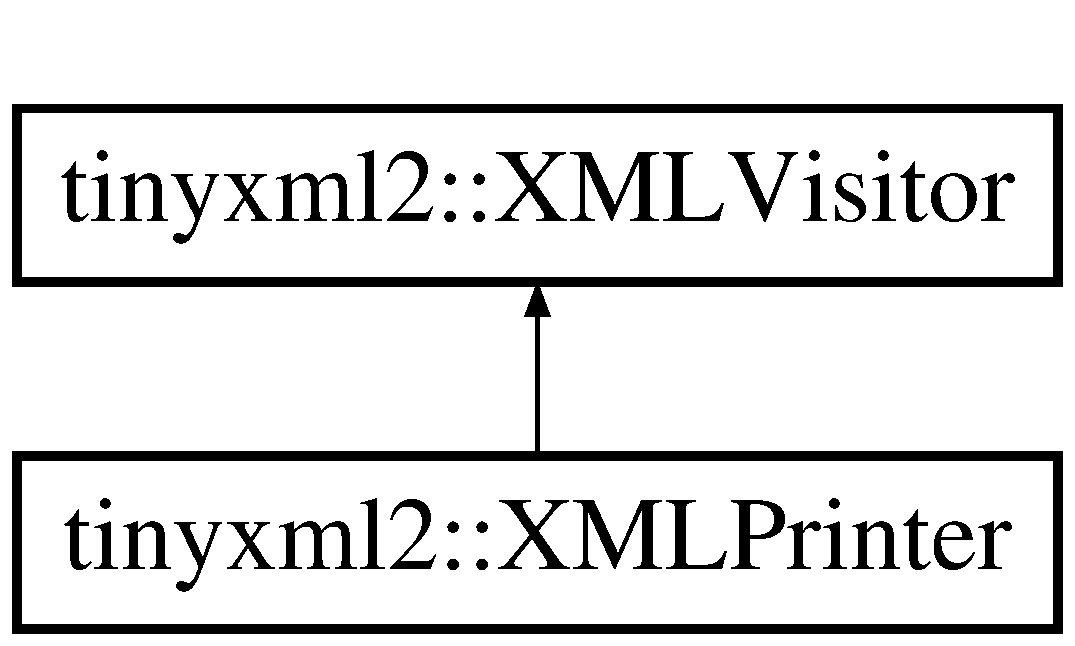
\includegraphics[height=2.000000cm]{classtinyxml2_1_1_x_m_l_printer}
\end{center}
\end{figure}
\subsection*{Public Member Functions}
\begin{DoxyCompactItemize}
\item 
\hyperlink{classtinyxml2_1_1_x_m_l_printer_aa6d3841c069085f5b8a27bc7103c04f7}{X\+M\+L\+Printer} (F\+I\+LE $\ast$file=0, bool compact=false, int depth=0)
\item 
virtual \hyperlink{classtinyxml2_1_1_x_m_l_printer_af4caefa48ea6436898fb1807de8d14c0}{$\sim$\+X\+M\+L\+Printer} ()
\item 
void \hyperlink{classtinyxml2_1_1_x_m_l_printer_a178c608ce8476043d5d6513819cde903}{Push\+Header} (bool write\+B\+OM, bool write\+Declaration)
\item 
void \hyperlink{classtinyxml2_1_1_x_m_l_printer_a20fb06c83bd13e5140d7dd13af06c010}{Open\+Element} (const char $\ast$name, bool compact\+Mode=false)
\item 
void \hyperlink{classtinyxml2_1_1_x_m_l_printer_a9a4e2c9348b42e147629d5a99f4af3f0}{Push\+Attribute} (const char $\ast$name, const char $\ast$value)
\begin{DoxyCompactList}\small\item\em If streaming, add an attribute to an open element. \end{DoxyCompactList}\item 
void \hyperlink{classtinyxml2_1_1_x_m_l_printer_a69120c82088597372d28d0a98f2ee7a1}{Push\+Attribute} (const char $\ast$name, int value)
\item 
void \hyperlink{classtinyxml2_1_1_x_m_l_printer_aa41039e51990aaf5342f3e0575a692c4}{Push\+Attribute} (const char $\ast$name, unsigned value)
\item 
void \hyperlink{classtinyxml2_1_1_x_m_l_printer_a9bc2fe21a83a70e6aa0415f2034ecbff}{Push\+Attribute} (const char $\ast$name, int64\+\_\+t value)
\item 
void \hyperlink{classtinyxml2_1_1_x_m_l_printer_a51f7950d7b7a19f0d3a0d549a318d45f}{Push\+Attribute} (const char $\ast$name, bool value)
\item 
void \hyperlink{classtinyxml2_1_1_x_m_l_printer_a1714867af40e68ca404c3e84b6cac2a6}{Push\+Attribute} (const char $\ast$name, double value)
\item 
virtual void \hyperlink{classtinyxml2_1_1_x_m_l_printer_af1fb439e5d800999646f333fa2f0699a}{Close\+Element} (bool compact\+Mode=false)
\begin{DoxyCompactList}\small\item\em If streaming, close the Element. \end{DoxyCompactList}\item 
void \hyperlink{classtinyxml2_1_1_x_m_l_printer_a1cc16a9362df4332012cb13cff6441b3}{Push\+Text} (const char $\ast$text, bool cdata=false)
\begin{DoxyCompactList}\small\item\em Add a text node. \end{DoxyCompactList}\item 
void \hyperlink{classtinyxml2_1_1_x_m_l_printer_a3e0d4d78de25d4cf081009e1431cea7e}{Push\+Text} (int value)
\begin{DoxyCompactList}\small\item\em Add a text node from an integer. \end{DoxyCompactList}\item 
void \hyperlink{classtinyxml2_1_1_x_m_l_printer_a661fb50e7e0a4918d2d259cb0fae647e}{Push\+Text} (unsigned value)
\begin{DoxyCompactList}\small\item\em Add a text node from an unsigned. \end{DoxyCompactList}\item 
void \hyperlink{classtinyxml2_1_1_x_m_l_printer_a96b0a0bfe105154a0a6c37d725258f0a}{Push\+Text} (int64\+\_\+t value)
\begin{DoxyCompactList}\small\item\em Add a text node from an unsigned. \end{DoxyCompactList}\item 
void \hyperlink{classtinyxml2_1_1_x_m_l_printer_a4390e5fa1ed05189a8686647345ab29f}{Push\+Text} (bool value)
\begin{DoxyCompactList}\small\item\em Add a text node from a bool. \end{DoxyCompactList}\item 
void \hyperlink{classtinyxml2_1_1_x_m_l_printer_a1dbb1390e829d0673af66b9cd1928bd7}{Push\+Text} (float value)
\begin{DoxyCompactList}\small\item\em Add a text node from a float. \end{DoxyCompactList}\item 
void \hyperlink{classtinyxml2_1_1_x_m_l_printer_aa715302dfc09473c77c853cbd5431965}{Push\+Text} (double value)
\begin{DoxyCompactList}\small\item\em Add a text node from a double. \end{DoxyCompactList}\item 
void \hyperlink{classtinyxml2_1_1_x_m_l_printer_afc8416814219591c2fd5656e0c233140}{Push\+Comment} (const char $\ast$comment)
\begin{DoxyCompactList}\small\item\em Add a comment. \end{DoxyCompactList}\item 
void \hyperlink{classtinyxml2_1_1_x_m_l_printer_a2fe3565e262594efc6c0276723c83fe7}{Push\+Declaration} (const char $\ast$value)
\item 
void \hyperlink{classtinyxml2_1_1_x_m_l_printer_ab1efc6d1548505e9984185f58f54b713}{Push\+Unknown} (const char $\ast$value)
\item 
virtual bool \hyperlink{classtinyxml2_1_1_x_m_l_printer_a9aa1de11a55a07db55a90fde37d7afad}{Visit\+Enter} (const \hyperlink{classtinyxml2_1_1_x_m_l_document}{X\+M\+L\+Document} \&)
\begin{DoxyCompactList}\small\item\em Visit a document. \end{DoxyCompactList}\item 
virtual bool \hyperlink{classtinyxml2_1_1_x_m_l_printer_a15fc1f2b922f540917dcf52808737b29}{Visit\+Exit} (const \hyperlink{classtinyxml2_1_1_x_m_l_document}{X\+M\+L\+Document} \&)
\begin{DoxyCompactList}\small\item\em Visit a document. \end{DoxyCompactList}\item 
virtual bool \hyperlink{classtinyxml2_1_1_x_m_l_printer_a169b2509d8eabb70811b2bb8cfd1f5d1}{Visit\+Enter} (const \hyperlink{classtinyxml2_1_1_x_m_l_element}{X\+M\+L\+Element} \&element, const \hyperlink{classtinyxml2_1_1_x_m_l_attribute}{X\+M\+L\+Attribute} $\ast$attribute)
\begin{DoxyCompactList}\small\item\em Visit an element. \end{DoxyCompactList}\item 
virtual bool \hyperlink{classtinyxml2_1_1_x_m_l_printer_a2edd48405971a88951c71c9df86a2f50}{Visit\+Exit} (const \hyperlink{classtinyxml2_1_1_x_m_l_element}{X\+M\+L\+Element} \&element)
\begin{DoxyCompactList}\small\item\em Visit an element. \end{DoxyCompactList}\item 
virtual bool \hyperlink{classtinyxml2_1_1_x_m_l_printer_adc0e42b4f6fcb90a95630c79575d030b}{Visit} (const \hyperlink{classtinyxml2_1_1_x_m_l_text}{X\+M\+L\+Text} \&text)
\begin{DoxyCompactList}\small\item\em Visit a text node. \end{DoxyCompactList}\item 
virtual bool \hyperlink{classtinyxml2_1_1_x_m_l_printer_aa294c5c01af0ebb9114902456e4cb53c}{Visit} (const \hyperlink{classtinyxml2_1_1_x_m_l_comment}{X\+M\+L\+Comment} \&comment)
\begin{DoxyCompactList}\small\item\em Visit a comment node. \end{DoxyCompactList}\item 
virtual bool \hyperlink{classtinyxml2_1_1_x_m_l_printer_acfc625b2549304b9c7eb85ebd5c5eb39}{Visit} (const \hyperlink{classtinyxml2_1_1_x_m_l_declaration}{X\+M\+L\+Declaration} \&declaration)
\begin{DoxyCompactList}\small\item\em Visit a declaration. \end{DoxyCompactList}\item 
virtual bool \hyperlink{classtinyxml2_1_1_x_m_l_printer_ab8af5455bbf9e4be2663e6642fcd7e32}{Visit} (const \hyperlink{classtinyxml2_1_1_x_m_l_unknown}{X\+M\+L\+Unknown} \&unknown)
\begin{DoxyCompactList}\small\item\em Visit an unknown node. \end{DoxyCompactList}\item 
const char $\ast$ \hyperlink{classtinyxml2_1_1_x_m_l_printer_a180671d73844f159f2d4aafbc11d106e}{C\+Str} () const
\item 
int \hyperlink{classtinyxml2_1_1_x_m_l_printer_a3256cf3523d4898b91abb18b924be04c}{C\+Str\+Size} () const
\item 
void \hyperlink{classtinyxml2_1_1_x_m_l_printer_a216157765b7267bf389975b1cbf9a909}{Clear\+Buffer} ()
\end{DoxyCompactItemize}
\subsection*{Protected Member Functions}
\begin{DoxyCompactItemize}
\item 
virtual bool \hyperlink{classtinyxml2_1_1_x_m_l_printer_a38e1ed5a779bdf63eda9e808f7a6de66}{Compact\+Mode} (const \hyperlink{classtinyxml2_1_1_x_m_l_element}{X\+M\+L\+Element} \&)
\item 
virtual void \hyperlink{classtinyxml2_1_1_x_m_l_printer_a1c4b2ccbe4fdb316d54f5a93f3559260}{Print\+Space} (int depth)
\item 
void \hyperlink{classtinyxml2_1_1_x_m_l_printer_ab30210a7f32e45634e7a45137bf6fdf6}{Print} (const char $\ast$format,...)
\item 
void \hyperlink{classtinyxml2_1_1_x_m_l_printer_ac6e2c72c5d796f5b4de6ce81ca95e3fa}{Seal\+Element\+If\+Just\+Opened} ()
\end{DoxyCompactItemize}
\subsection*{Protected Attributes}
\begin{DoxyCompactItemize}
\item 
bool \hyperlink{classtinyxml2_1_1_x_m_l_printer_ac07169d58b465214a2b1fa306e617c26}{\+\_\+element\+Just\+Opened}
\item 
\hyperlink{classtinyxml2_1_1_dyn_array}{Dyn\+Array}$<$ const char $\ast$, 10 $>$ \hyperlink{classtinyxml2_1_1_x_m_l_printer_a99d59e67e084714541bee3ae43884bef}{\+\_\+stack}
\end{DoxyCompactItemize}


\subsection{Detailed Description}
Printing functionality. The \hyperlink{classtinyxml2_1_1_x_m_l_printer}{X\+M\+L\+Printer} gives you more options than the \hyperlink{classtinyxml2_1_1_x_m_l_document_a867cf5fa3e3ff6ae4847a8b7ee8ec083}{X\+M\+L\+Document\+::\+Print()} method.

It can\+:
\begin{DoxyEnumerate}
\item Print to memory.
\item Print to a file you provide.
\item Print X\+ML without a \hyperlink{classtinyxml2_1_1_x_m_l_document}{X\+M\+L\+Document}.
\end{DoxyEnumerate}

Print to Memory

\begin{DoxyVerb}XMLPrinter printer;
doc.Print( &printer );
SomeFunction( printer.CStr() );
\end{DoxyVerb}


Print to a File

You provide the file pointer. \begin{DoxyVerb}XMLPrinter printer( fp );
doc.Print( &printer );
\end{DoxyVerb}


Print without a \hyperlink{classtinyxml2_1_1_x_m_l_document}{X\+M\+L\+Document}

When loading, an X\+ML parser is very useful. However, sometimes when saving, it just gets in the way. The code is often set up for streaming, and constructing the D\+OM is just overhead.

The Printer supports the streaming case. The following code prints out a trivially simple X\+ML file without ever creating an X\+ML document.

\begin{DoxyVerb}XMLPrinter printer( fp );
printer.OpenElement( "foo" );
printer.PushAttribute( "foo", "bar" );
printer.CloseElement();
\end{DoxyVerb}
 

\subsection{Constructor \& Destructor Documentation}
\mbox{\Hypertarget{classtinyxml2_1_1_x_m_l_printer_aa6d3841c069085f5b8a27bc7103c04f7}\label{classtinyxml2_1_1_x_m_l_printer_aa6d3841c069085f5b8a27bc7103c04f7}} 
\index{tinyxml2\+::\+X\+M\+L\+Printer@{tinyxml2\+::\+X\+M\+L\+Printer}!X\+M\+L\+Printer@{X\+M\+L\+Printer}}
\index{X\+M\+L\+Printer@{X\+M\+L\+Printer}!tinyxml2\+::\+X\+M\+L\+Printer@{tinyxml2\+::\+X\+M\+L\+Printer}}
\subsubsection{\texorpdfstring{X\+M\+L\+Printer()}{XMLPrinter()}}
{\footnotesize\ttfamily tinyxml2\+::\+X\+M\+L\+Printer\+::\+X\+M\+L\+Printer (\begin{DoxyParamCaption}\item[{F\+I\+LE $\ast$}]{file = {\ttfamily 0},  }\item[{bool}]{compact = {\ttfamily false},  }\item[{int}]{depth = {\ttfamily 0} }\end{DoxyParamCaption})}

Construct the printer. If the F\+I\+L\+E$\ast$ is specified, this will print to the F\+I\+LE. Else it will print to memory, and the result is available in \hyperlink{classtinyxml2_1_1_x_m_l_printer_a180671d73844f159f2d4aafbc11d106e}{C\+Str()}. If \textquotesingle{}compact\textquotesingle{} is set to true, then output is created with only required whitespace and newlines. \mbox{\Hypertarget{classtinyxml2_1_1_x_m_l_printer_af4caefa48ea6436898fb1807de8d14c0}\label{classtinyxml2_1_1_x_m_l_printer_af4caefa48ea6436898fb1807de8d14c0}} 
\index{tinyxml2\+::\+X\+M\+L\+Printer@{tinyxml2\+::\+X\+M\+L\+Printer}!````~X\+M\+L\+Printer@{$\sim$\+X\+M\+L\+Printer}}
\index{````~X\+M\+L\+Printer@{$\sim$\+X\+M\+L\+Printer}!tinyxml2\+::\+X\+M\+L\+Printer@{tinyxml2\+::\+X\+M\+L\+Printer}}
\subsubsection{\texorpdfstring{$\sim$\+X\+M\+L\+Printer()}{~XMLPrinter()}}
{\footnotesize\ttfamily virtual tinyxml2\+::\+X\+M\+L\+Printer\+::$\sim$\+X\+M\+L\+Printer (\begin{DoxyParamCaption}{ }\end{DoxyParamCaption})\hspace{0.3cm}{\ttfamily [inline]}, {\ttfamily [virtual]}}



\subsection{Member Function Documentation}
\mbox{\Hypertarget{classtinyxml2_1_1_x_m_l_printer_a216157765b7267bf389975b1cbf9a909}\label{classtinyxml2_1_1_x_m_l_printer_a216157765b7267bf389975b1cbf9a909}} 
\index{tinyxml2\+::\+X\+M\+L\+Printer@{tinyxml2\+::\+X\+M\+L\+Printer}!Clear\+Buffer@{Clear\+Buffer}}
\index{Clear\+Buffer@{Clear\+Buffer}!tinyxml2\+::\+X\+M\+L\+Printer@{tinyxml2\+::\+X\+M\+L\+Printer}}
\subsubsection{\texorpdfstring{Clear\+Buffer()}{ClearBuffer()}}
{\footnotesize\ttfamily void tinyxml2\+::\+X\+M\+L\+Printer\+::\+Clear\+Buffer (\begin{DoxyParamCaption}{ }\end{DoxyParamCaption})\hspace{0.3cm}{\ttfamily [inline]}}

If in print to memory mode, reset the buffer to the beginning. \mbox{\Hypertarget{classtinyxml2_1_1_x_m_l_printer_af1fb439e5d800999646f333fa2f0699a}\label{classtinyxml2_1_1_x_m_l_printer_af1fb439e5d800999646f333fa2f0699a}} 
\index{tinyxml2\+::\+X\+M\+L\+Printer@{tinyxml2\+::\+X\+M\+L\+Printer}!Close\+Element@{Close\+Element}}
\index{Close\+Element@{Close\+Element}!tinyxml2\+::\+X\+M\+L\+Printer@{tinyxml2\+::\+X\+M\+L\+Printer}}
\subsubsection{\texorpdfstring{Close\+Element()}{CloseElement()}}
{\footnotesize\ttfamily void tinyxml2\+::\+X\+M\+L\+Printer\+::\+Close\+Element (\begin{DoxyParamCaption}\item[{bool}]{compact\+Mode = {\ttfamily false} }\end{DoxyParamCaption})\hspace{0.3cm}{\ttfamily [virtual]}}



If streaming, close the Element. 

\mbox{\Hypertarget{classtinyxml2_1_1_x_m_l_printer_a38e1ed5a779bdf63eda9e808f7a6de66}\label{classtinyxml2_1_1_x_m_l_printer_a38e1ed5a779bdf63eda9e808f7a6de66}} 
\index{tinyxml2\+::\+X\+M\+L\+Printer@{tinyxml2\+::\+X\+M\+L\+Printer}!Compact\+Mode@{Compact\+Mode}}
\index{Compact\+Mode@{Compact\+Mode}!tinyxml2\+::\+X\+M\+L\+Printer@{tinyxml2\+::\+X\+M\+L\+Printer}}
\subsubsection{\texorpdfstring{Compact\+Mode()}{CompactMode()}}
{\footnotesize\ttfamily virtual bool tinyxml2\+::\+X\+M\+L\+Printer\+::\+Compact\+Mode (\begin{DoxyParamCaption}\item[{const \hyperlink{classtinyxml2_1_1_x_m_l_element}{X\+M\+L\+Element} \&}]{ }\end{DoxyParamCaption})\hspace{0.3cm}{\ttfamily [inline]}, {\ttfamily [protected]}, {\ttfamily [virtual]}}

\mbox{\Hypertarget{classtinyxml2_1_1_x_m_l_printer_a180671d73844f159f2d4aafbc11d106e}\label{classtinyxml2_1_1_x_m_l_printer_a180671d73844f159f2d4aafbc11d106e}} 
\index{tinyxml2\+::\+X\+M\+L\+Printer@{tinyxml2\+::\+X\+M\+L\+Printer}!C\+Str@{C\+Str}}
\index{C\+Str@{C\+Str}!tinyxml2\+::\+X\+M\+L\+Printer@{tinyxml2\+::\+X\+M\+L\+Printer}}
\subsubsection{\texorpdfstring{C\+Str()}{CStr()}}
{\footnotesize\ttfamily const char$\ast$ tinyxml2\+::\+X\+M\+L\+Printer\+::\+C\+Str (\begin{DoxyParamCaption}{ }\end{DoxyParamCaption}) const\hspace{0.3cm}{\ttfamily [inline]}}

If in print to memory mode, return a pointer to the X\+ML file in memory. \mbox{\Hypertarget{classtinyxml2_1_1_x_m_l_printer_a3256cf3523d4898b91abb18b924be04c}\label{classtinyxml2_1_1_x_m_l_printer_a3256cf3523d4898b91abb18b924be04c}} 
\index{tinyxml2\+::\+X\+M\+L\+Printer@{tinyxml2\+::\+X\+M\+L\+Printer}!C\+Str\+Size@{C\+Str\+Size}}
\index{C\+Str\+Size@{C\+Str\+Size}!tinyxml2\+::\+X\+M\+L\+Printer@{tinyxml2\+::\+X\+M\+L\+Printer}}
\subsubsection{\texorpdfstring{C\+Str\+Size()}{CStrSize()}}
{\footnotesize\ttfamily int tinyxml2\+::\+X\+M\+L\+Printer\+::\+C\+Str\+Size (\begin{DoxyParamCaption}{ }\end{DoxyParamCaption}) const\hspace{0.3cm}{\ttfamily [inline]}}

If in print to memory mode, return the size of the X\+ML file in memory. (Note the size returned includes the terminating null.) \mbox{\Hypertarget{classtinyxml2_1_1_x_m_l_printer_a20fb06c83bd13e5140d7dd13af06c010}\label{classtinyxml2_1_1_x_m_l_printer_a20fb06c83bd13e5140d7dd13af06c010}} 
\index{tinyxml2\+::\+X\+M\+L\+Printer@{tinyxml2\+::\+X\+M\+L\+Printer}!Open\+Element@{Open\+Element}}
\index{Open\+Element@{Open\+Element}!tinyxml2\+::\+X\+M\+L\+Printer@{tinyxml2\+::\+X\+M\+L\+Printer}}
\subsubsection{\texorpdfstring{Open\+Element()}{OpenElement()}}
{\footnotesize\ttfamily void tinyxml2\+::\+X\+M\+L\+Printer\+::\+Open\+Element (\begin{DoxyParamCaption}\item[{const char $\ast$}]{name,  }\item[{bool}]{compact\+Mode = {\ttfamily false} }\end{DoxyParamCaption})}

If streaming, start writing an element. The element must be closed with \hyperlink{classtinyxml2_1_1_x_m_l_printer_af1fb439e5d800999646f333fa2f0699a}{Close\+Element()} \mbox{\Hypertarget{classtinyxml2_1_1_x_m_l_printer_ab30210a7f32e45634e7a45137bf6fdf6}\label{classtinyxml2_1_1_x_m_l_printer_ab30210a7f32e45634e7a45137bf6fdf6}} 
\index{tinyxml2\+::\+X\+M\+L\+Printer@{tinyxml2\+::\+X\+M\+L\+Printer}!Print@{Print}}
\index{Print@{Print}!tinyxml2\+::\+X\+M\+L\+Printer@{tinyxml2\+::\+X\+M\+L\+Printer}}
\subsubsection{\texorpdfstring{Print()}{Print()}}
{\footnotesize\ttfamily void tinyxml2\+::\+X\+M\+L\+Printer\+::\+Print (\begin{DoxyParamCaption}\item[{const char $\ast$}]{format,  }\item[{}]{... }\end{DoxyParamCaption})\hspace{0.3cm}{\ttfamily [protected]}}

\mbox{\Hypertarget{classtinyxml2_1_1_x_m_l_printer_a1c4b2ccbe4fdb316d54f5a93f3559260}\label{classtinyxml2_1_1_x_m_l_printer_a1c4b2ccbe4fdb316d54f5a93f3559260}} 
\index{tinyxml2\+::\+X\+M\+L\+Printer@{tinyxml2\+::\+X\+M\+L\+Printer}!Print\+Space@{Print\+Space}}
\index{Print\+Space@{Print\+Space}!tinyxml2\+::\+X\+M\+L\+Printer@{tinyxml2\+::\+X\+M\+L\+Printer}}
\subsubsection{\texorpdfstring{Print\+Space()}{PrintSpace()}}
{\footnotesize\ttfamily void tinyxml2\+::\+X\+M\+L\+Printer\+::\+Print\+Space (\begin{DoxyParamCaption}\item[{int}]{depth }\end{DoxyParamCaption})\hspace{0.3cm}{\ttfamily [protected]}, {\ttfamily [virtual]}}

Prints out the space before an element. You may override to change the space and tabs used. A \hyperlink{classtinyxml2_1_1_x_m_l_printer_a1c4b2ccbe4fdb316d54f5a93f3559260}{Print\+Space()} override should call \hyperlink{classtinyxml2_1_1_x_m_l_printer_ab30210a7f32e45634e7a45137bf6fdf6}{Print()}. \mbox{\Hypertarget{classtinyxml2_1_1_x_m_l_printer_a9a4e2c9348b42e147629d5a99f4af3f0}\label{classtinyxml2_1_1_x_m_l_printer_a9a4e2c9348b42e147629d5a99f4af3f0}} 
\index{tinyxml2\+::\+X\+M\+L\+Printer@{tinyxml2\+::\+X\+M\+L\+Printer}!Push\+Attribute@{Push\+Attribute}}
\index{Push\+Attribute@{Push\+Attribute}!tinyxml2\+::\+X\+M\+L\+Printer@{tinyxml2\+::\+X\+M\+L\+Printer}}
\subsubsection{\texorpdfstring{Push\+Attribute()}{PushAttribute()}\hspace{0.1cm}{\footnotesize\ttfamily [1/6]}}
{\footnotesize\ttfamily void tinyxml2\+::\+X\+M\+L\+Printer\+::\+Push\+Attribute (\begin{DoxyParamCaption}\item[{const char $\ast$}]{name,  }\item[{const char $\ast$}]{value }\end{DoxyParamCaption})}



If streaming, add an attribute to an open element. 

\mbox{\Hypertarget{classtinyxml2_1_1_x_m_l_printer_a69120c82088597372d28d0a98f2ee7a1}\label{classtinyxml2_1_1_x_m_l_printer_a69120c82088597372d28d0a98f2ee7a1}} 
\index{tinyxml2\+::\+X\+M\+L\+Printer@{tinyxml2\+::\+X\+M\+L\+Printer}!Push\+Attribute@{Push\+Attribute}}
\index{Push\+Attribute@{Push\+Attribute}!tinyxml2\+::\+X\+M\+L\+Printer@{tinyxml2\+::\+X\+M\+L\+Printer}}
\subsubsection{\texorpdfstring{Push\+Attribute()}{PushAttribute()}\hspace{0.1cm}{\footnotesize\ttfamily [2/6]}}
{\footnotesize\ttfamily void tinyxml2\+::\+X\+M\+L\+Printer\+::\+Push\+Attribute (\begin{DoxyParamCaption}\item[{const char $\ast$}]{name,  }\item[{int}]{value }\end{DoxyParamCaption})}

\mbox{\Hypertarget{classtinyxml2_1_1_x_m_l_printer_aa41039e51990aaf5342f3e0575a692c4}\label{classtinyxml2_1_1_x_m_l_printer_aa41039e51990aaf5342f3e0575a692c4}} 
\index{tinyxml2\+::\+X\+M\+L\+Printer@{tinyxml2\+::\+X\+M\+L\+Printer}!Push\+Attribute@{Push\+Attribute}}
\index{Push\+Attribute@{Push\+Attribute}!tinyxml2\+::\+X\+M\+L\+Printer@{tinyxml2\+::\+X\+M\+L\+Printer}}
\subsubsection{\texorpdfstring{Push\+Attribute()}{PushAttribute()}\hspace{0.1cm}{\footnotesize\ttfamily [3/6]}}
{\footnotesize\ttfamily void tinyxml2\+::\+X\+M\+L\+Printer\+::\+Push\+Attribute (\begin{DoxyParamCaption}\item[{const char $\ast$}]{name,  }\item[{unsigned}]{value }\end{DoxyParamCaption})}

\mbox{\Hypertarget{classtinyxml2_1_1_x_m_l_printer_a9bc2fe21a83a70e6aa0415f2034ecbff}\label{classtinyxml2_1_1_x_m_l_printer_a9bc2fe21a83a70e6aa0415f2034ecbff}} 
\index{tinyxml2\+::\+X\+M\+L\+Printer@{tinyxml2\+::\+X\+M\+L\+Printer}!Push\+Attribute@{Push\+Attribute}}
\index{Push\+Attribute@{Push\+Attribute}!tinyxml2\+::\+X\+M\+L\+Printer@{tinyxml2\+::\+X\+M\+L\+Printer}}
\subsubsection{\texorpdfstring{Push\+Attribute()}{PushAttribute()}\hspace{0.1cm}{\footnotesize\ttfamily [4/6]}}
{\footnotesize\ttfamily void tinyxml2\+::\+X\+M\+L\+Printer\+::\+Push\+Attribute (\begin{DoxyParamCaption}\item[{const char $\ast$}]{name,  }\item[{int64\+\_\+t}]{value }\end{DoxyParamCaption})}

\mbox{\Hypertarget{classtinyxml2_1_1_x_m_l_printer_a51f7950d7b7a19f0d3a0d549a318d45f}\label{classtinyxml2_1_1_x_m_l_printer_a51f7950d7b7a19f0d3a0d549a318d45f}} 
\index{tinyxml2\+::\+X\+M\+L\+Printer@{tinyxml2\+::\+X\+M\+L\+Printer}!Push\+Attribute@{Push\+Attribute}}
\index{Push\+Attribute@{Push\+Attribute}!tinyxml2\+::\+X\+M\+L\+Printer@{tinyxml2\+::\+X\+M\+L\+Printer}}
\subsubsection{\texorpdfstring{Push\+Attribute()}{PushAttribute()}\hspace{0.1cm}{\footnotesize\ttfamily [5/6]}}
{\footnotesize\ttfamily void tinyxml2\+::\+X\+M\+L\+Printer\+::\+Push\+Attribute (\begin{DoxyParamCaption}\item[{const char $\ast$}]{name,  }\item[{bool}]{value }\end{DoxyParamCaption})}

\mbox{\Hypertarget{classtinyxml2_1_1_x_m_l_printer_a1714867af40e68ca404c3e84b6cac2a6}\label{classtinyxml2_1_1_x_m_l_printer_a1714867af40e68ca404c3e84b6cac2a6}} 
\index{tinyxml2\+::\+X\+M\+L\+Printer@{tinyxml2\+::\+X\+M\+L\+Printer}!Push\+Attribute@{Push\+Attribute}}
\index{Push\+Attribute@{Push\+Attribute}!tinyxml2\+::\+X\+M\+L\+Printer@{tinyxml2\+::\+X\+M\+L\+Printer}}
\subsubsection{\texorpdfstring{Push\+Attribute()}{PushAttribute()}\hspace{0.1cm}{\footnotesize\ttfamily [6/6]}}
{\footnotesize\ttfamily void tinyxml2\+::\+X\+M\+L\+Printer\+::\+Push\+Attribute (\begin{DoxyParamCaption}\item[{const char $\ast$}]{name,  }\item[{double}]{value }\end{DoxyParamCaption})}

\mbox{\Hypertarget{classtinyxml2_1_1_x_m_l_printer_afc8416814219591c2fd5656e0c233140}\label{classtinyxml2_1_1_x_m_l_printer_afc8416814219591c2fd5656e0c233140}} 
\index{tinyxml2\+::\+X\+M\+L\+Printer@{tinyxml2\+::\+X\+M\+L\+Printer}!Push\+Comment@{Push\+Comment}}
\index{Push\+Comment@{Push\+Comment}!tinyxml2\+::\+X\+M\+L\+Printer@{tinyxml2\+::\+X\+M\+L\+Printer}}
\subsubsection{\texorpdfstring{Push\+Comment()}{PushComment()}}
{\footnotesize\ttfamily void tinyxml2\+::\+X\+M\+L\+Printer\+::\+Push\+Comment (\begin{DoxyParamCaption}\item[{const char $\ast$}]{comment }\end{DoxyParamCaption})}



Add a comment. 

\mbox{\Hypertarget{classtinyxml2_1_1_x_m_l_printer_a2fe3565e262594efc6c0276723c83fe7}\label{classtinyxml2_1_1_x_m_l_printer_a2fe3565e262594efc6c0276723c83fe7}} 
\index{tinyxml2\+::\+X\+M\+L\+Printer@{tinyxml2\+::\+X\+M\+L\+Printer}!Push\+Declaration@{Push\+Declaration}}
\index{Push\+Declaration@{Push\+Declaration}!tinyxml2\+::\+X\+M\+L\+Printer@{tinyxml2\+::\+X\+M\+L\+Printer}}
\subsubsection{\texorpdfstring{Push\+Declaration()}{PushDeclaration()}}
{\footnotesize\ttfamily void tinyxml2\+::\+X\+M\+L\+Printer\+::\+Push\+Declaration (\begin{DoxyParamCaption}\item[{const char $\ast$}]{value }\end{DoxyParamCaption})}

\mbox{\Hypertarget{classtinyxml2_1_1_x_m_l_printer_a178c608ce8476043d5d6513819cde903}\label{classtinyxml2_1_1_x_m_l_printer_a178c608ce8476043d5d6513819cde903}} 
\index{tinyxml2\+::\+X\+M\+L\+Printer@{tinyxml2\+::\+X\+M\+L\+Printer}!Push\+Header@{Push\+Header}}
\index{Push\+Header@{Push\+Header}!tinyxml2\+::\+X\+M\+L\+Printer@{tinyxml2\+::\+X\+M\+L\+Printer}}
\subsubsection{\texorpdfstring{Push\+Header()}{PushHeader()}}
{\footnotesize\ttfamily void tinyxml2\+::\+X\+M\+L\+Printer\+::\+Push\+Header (\begin{DoxyParamCaption}\item[{bool}]{write\+B\+OM,  }\item[{bool}]{write\+Declaration }\end{DoxyParamCaption})}

If streaming, write the B\+OM and declaration. \mbox{\Hypertarget{classtinyxml2_1_1_x_m_l_printer_a1cc16a9362df4332012cb13cff6441b3}\label{classtinyxml2_1_1_x_m_l_printer_a1cc16a9362df4332012cb13cff6441b3}} 
\index{tinyxml2\+::\+X\+M\+L\+Printer@{tinyxml2\+::\+X\+M\+L\+Printer}!Push\+Text@{Push\+Text}}
\index{Push\+Text@{Push\+Text}!tinyxml2\+::\+X\+M\+L\+Printer@{tinyxml2\+::\+X\+M\+L\+Printer}}
\subsubsection{\texorpdfstring{Push\+Text()}{PushText()}\hspace{0.1cm}{\footnotesize\ttfamily [1/7]}}
{\footnotesize\ttfamily void tinyxml2\+::\+X\+M\+L\+Printer\+::\+Push\+Text (\begin{DoxyParamCaption}\item[{const char $\ast$}]{text,  }\item[{bool}]{cdata = {\ttfamily false} }\end{DoxyParamCaption})}



Add a text node. 

\mbox{\Hypertarget{classtinyxml2_1_1_x_m_l_printer_a3e0d4d78de25d4cf081009e1431cea7e}\label{classtinyxml2_1_1_x_m_l_printer_a3e0d4d78de25d4cf081009e1431cea7e}} 
\index{tinyxml2\+::\+X\+M\+L\+Printer@{tinyxml2\+::\+X\+M\+L\+Printer}!Push\+Text@{Push\+Text}}
\index{Push\+Text@{Push\+Text}!tinyxml2\+::\+X\+M\+L\+Printer@{tinyxml2\+::\+X\+M\+L\+Printer}}
\subsubsection{\texorpdfstring{Push\+Text()}{PushText()}\hspace{0.1cm}{\footnotesize\ttfamily [2/7]}}
{\footnotesize\ttfamily void tinyxml2\+::\+X\+M\+L\+Printer\+::\+Push\+Text (\begin{DoxyParamCaption}\item[{int}]{value }\end{DoxyParamCaption})}



Add a text node from an integer. 

\mbox{\Hypertarget{classtinyxml2_1_1_x_m_l_printer_a661fb50e7e0a4918d2d259cb0fae647e}\label{classtinyxml2_1_1_x_m_l_printer_a661fb50e7e0a4918d2d259cb0fae647e}} 
\index{tinyxml2\+::\+X\+M\+L\+Printer@{tinyxml2\+::\+X\+M\+L\+Printer}!Push\+Text@{Push\+Text}}
\index{Push\+Text@{Push\+Text}!tinyxml2\+::\+X\+M\+L\+Printer@{tinyxml2\+::\+X\+M\+L\+Printer}}
\subsubsection{\texorpdfstring{Push\+Text()}{PushText()}\hspace{0.1cm}{\footnotesize\ttfamily [3/7]}}
{\footnotesize\ttfamily void tinyxml2\+::\+X\+M\+L\+Printer\+::\+Push\+Text (\begin{DoxyParamCaption}\item[{unsigned}]{value }\end{DoxyParamCaption})}



Add a text node from an unsigned. 

\mbox{\Hypertarget{classtinyxml2_1_1_x_m_l_printer_a96b0a0bfe105154a0a6c37d725258f0a}\label{classtinyxml2_1_1_x_m_l_printer_a96b0a0bfe105154a0a6c37d725258f0a}} 
\index{tinyxml2\+::\+X\+M\+L\+Printer@{tinyxml2\+::\+X\+M\+L\+Printer}!Push\+Text@{Push\+Text}}
\index{Push\+Text@{Push\+Text}!tinyxml2\+::\+X\+M\+L\+Printer@{tinyxml2\+::\+X\+M\+L\+Printer}}
\subsubsection{\texorpdfstring{Push\+Text()}{PushText()}\hspace{0.1cm}{\footnotesize\ttfamily [4/7]}}
{\footnotesize\ttfamily void tinyxml2\+::\+X\+M\+L\+Printer\+::\+Push\+Text (\begin{DoxyParamCaption}\item[{int64\+\_\+t}]{value }\end{DoxyParamCaption})}



Add a text node from an unsigned. 

\mbox{\Hypertarget{classtinyxml2_1_1_x_m_l_printer_a4390e5fa1ed05189a8686647345ab29f}\label{classtinyxml2_1_1_x_m_l_printer_a4390e5fa1ed05189a8686647345ab29f}} 
\index{tinyxml2\+::\+X\+M\+L\+Printer@{tinyxml2\+::\+X\+M\+L\+Printer}!Push\+Text@{Push\+Text}}
\index{Push\+Text@{Push\+Text}!tinyxml2\+::\+X\+M\+L\+Printer@{tinyxml2\+::\+X\+M\+L\+Printer}}
\subsubsection{\texorpdfstring{Push\+Text()}{PushText()}\hspace{0.1cm}{\footnotesize\ttfamily [5/7]}}
{\footnotesize\ttfamily void tinyxml2\+::\+X\+M\+L\+Printer\+::\+Push\+Text (\begin{DoxyParamCaption}\item[{bool}]{value }\end{DoxyParamCaption})}



Add a text node from a bool. 

\mbox{\Hypertarget{classtinyxml2_1_1_x_m_l_printer_a1dbb1390e829d0673af66b9cd1928bd7}\label{classtinyxml2_1_1_x_m_l_printer_a1dbb1390e829d0673af66b9cd1928bd7}} 
\index{tinyxml2\+::\+X\+M\+L\+Printer@{tinyxml2\+::\+X\+M\+L\+Printer}!Push\+Text@{Push\+Text}}
\index{Push\+Text@{Push\+Text}!tinyxml2\+::\+X\+M\+L\+Printer@{tinyxml2\+::\+X\+M\+L\+Printer}}
\subsubsection{\texorpdfstring{Push\+Text()}{PushText()}\hspace{0.1cm}{\footnotesize\ttfamily [6/7]}}
{\footnotesize\ttfamily void tinyxml2\+::\+X\+M\+L\+Printer\+::\+Push\+Text (\begin{DoxyParamCaption}\item[{float}]{value }\end{DoxyParamCaption})}



Add a text node from a float. 

\mbox{\Hypertarget{classtinyxml2_1_1_x_m_l_printer_aa715302dfc09473c77c853cbd5431965}\label{classtinyxml2_1_1_x_m_l_printer_aa715302dfc09473c77c853cbd5431965}} 
\index{tinyxml2\+::\+X\+M\+L\+Printer@{tinyxml2\+::\+X\+M\+L\+Printer}!Push\+Text@{Push\+Text}}
\index{Push\+Text@{Push\+Text}!tinyxml2\+::\+X\+M\+L\+Printer@{tinyxml2\+::\+X\+M\+L\+Printer}}
\subsubsection{\texorpdfstring{Push\+Text()}{PushText()}\hspace{0.1cm}{\footnotesize\ttfamily [7/7]}}
{\footnotesize\ttfamily void tinyxml2\+::\+X\+M\+L\+Printer\+::\+Push\+Text (\begin{DoxyParamCaption}\item[{double}]{value }\end{DoxyParamCaption})}



Add a text node from a double. 

\mbox{\Hypertarget{classtinyxml2_1_1_x_m_l_printer_ab1efc6d1548505e9984185f58f54b713}\label{classtinyxml2_1_1_x_m_l_printer_ab1efc6d1548505e9984185f58f54b713}} 
\index{tinyxml2\+::\+X\+M\+L\+Printer@{tinyxml2\+::\+X\+M\+L\+Printer}!Push\+Unknown@{Push\+Unknown}}
\index{Push\+Unknown@{Push\+Unknown}!tinyxml2\+::\+X\+M\+L\+Printer@{tinyxml2\+::\+X\+M\+L\+Printer}}
\subsubsection{\texorpdfstring{Push\+Unknown()}{PushUnknown()}}
{\footnotesize\ttfamily void tinyxml2\+::\+X\+M\+L\+Printer\+::\+Push\+Unknown (\begin{DoxyParamCaption}\item[{const char $\ast$}]{value }\end{DoxyParamCaption})}

\mbox{\Hypertarget{classtinyxml2_1_1_x_m_l_printer_ac6e2c72c5d796f5b4de6ce81ca95e3fa}\label{classtinyxml2_1_1_x_m_l_printer_ac6e2c72c5d796f5b4de6ce81ca95e3fa}} 
\index{tinyxml2\+::\+X\+M\+L\+Printer@{tinyxml2\+::\+X\+M\+L\+Printer}!Seal\+Element\+If\+Just\+Opened@{Seal\+Element\+If\+Just\+Opened}}
\index{Seal\+Element\+If\+Just\+Opened@{Seal\+Element\+If\+Just\+Opened}!tinyxml2\+::\+X\+M\+L\+Printer@{tinyxml2\+::\+X\+M\+L\+Printer}}
\subsubsection{\texorpdfstring{Seal\+Element\+If\+Just\+Opened()}{SealElementIfJustOpened()}}
{\footnotesize\ttfamily void tinyxml2\+::\+X\+M\+L\+Printer\+::\+Seal\+Element\+If\+Just\+Opened (\begin{DoxyParamCaption}{ }\end{DoxyParamCaption})\hspace{0.3cm}{\ttfamily [protected]}}

\mbox{\Hypertarget{classtinyxml2_1_1_x_m_l_printer_adc0e42b4f6fcb90a95630c79575d030b}\label{classtinyxml2_1_1_x_m_l_printer_adc0e42b4f6fcb90a95630c79575d030b}} 
\index{tinyxml2\+::\+X\+M\+L\+Printer@{tinyxml2\+::\+X\+M\+L\+Printer}!Visit@{Visit}}
\index{Visit@{Visit}!tinyxml2\+::\+X\+M\+L\+Printer@{tinyxml2\+::\+X\+M\+L\+Printer}}
\subsubsection{\texorpdfstring{Visit()}{Visit()}\hspace{0.1cm}{\footnotesize\ttfamily [1/4]}}
{\footnotesize\ttfamily bool tinyxml2\+::\+X\+M\+L\+Printer\+::\+Visit (\begin{DoxyParamCaption}\item[{const \hyperlink{classtinyxml2_1_1_x_m_l_text}{X\+M\+L\+Text} \&}]{ }\end{DoxyParamCaption})\hspace{0.3cm}{\ttfamily [virtual]}}



Visit a text node. 



Reimplemented from \hyperlink{classtinyxml2_1_1_x_m_l_visitor_af30233565856480ea48b6fa0d6dec65b}{tinyxml2\+::\+X\+M\+L\+Visitor}.

\mbox{\Hypertarget{classtinyxml2_1_1_x_m_l_printer_aa294c5c01af0ebb9114902456e4cb53c}\label{classtinyxml2_1_1_x_m_l_printer_aa294c5c01af0ebb9114902456e4cb53c}} 
\index{tinyxml2\+::\+X\+M\+L\+Printer@{tinyxml2\+::\+X\+M\+L\+Printer}!Visit@{Visit}}
\index{Visit@{Visit}!tinyxml2\+::\+X\+M\+L\+Printer@{tinyxml2\+::\+X\+M\+L\+Printer}}
\subsubsection{\texorpdfstring{Visit()}{Visit()}\hspace{0.1cm}{\footnotesize\ttfamily [2/4]}}
{\footnotesize\ttfamily bool tinyxml2\+::\+X\+M\+L\+Printer\+::\+Visit (\begin{DoxyParamCaption}\item[{const \hyperlink{classtinyxml2_1_1_x_m_l_comment}{X\+M\+L\+Comment} \&}]{ }\end{DoxyParamCaption})\hspace{0.3cm}{\ttfamily [virtual]}}



Visit a comment node. 



Reimplemented from \hyperlink{classtinyxml2_1_1_x_m_l_visitor_acc8147fb5a85f6c65721654e427752d7}{tinyxml2\+::\+X\+M\+L\+Visitor}.

\mbox{\Hypertarget{classtinyxml2_1_1_x_m_l_printer_acfc625b2549304b9c7eb85ebd5c5eb39}\label{classtinyxml2_1_1_x_m_l_printer_acfc625b2549304b9c7eb85ebd5c5eb39}} 
\index{tinyxml2\+::\+X\+M\+L\+Printer@{tinyxml2\+::\+X\+M\+L\+Printer}!Visit@{Visit}}
\index{Visit@{Visit}!tinyxml2\+::\+X\+M\+L\+Printer@{tinyxml2\+::\+X\+M\+L\+Printer}}
\subsubsection{\texorpdfstring{Visit()}{Visit()}\hspace{0.1cm}{\footnotesize\ttfamily [3/4]}}
{\footnotesize\ttfamily bool tinyxml2\+::\+X\+M\+L\+Printer\+::\+Visit (\begin{DoxyParamCaption}\item[{const \hyperlink{classtinyxml2_1_1_x_m_l_declaration}{X\+M\+L\+Declaration} \&}]{ }\end{DoxyParamCaption})\hspace{0.3cm}{\ttfamily [virtual]}}



Visit a declaration. 



Reimplemented from \hyperlink{classtinyxml2_1_1_x_m_l_visitor_adc75bd459fc7ba8223b50f0616767f9a}{tinyxml2\+::\+X\+M\+L\+Visitor}.

\mbox{\Hypertarget{classtinyxml2_1_1_x_m_l_printer_ab8af5455bbf9e4be2663e6642fcd7e32}\label{classtinyxml2_1_1_x_m_l_printer_ab8af5455bbf9e4be2663e6642fcd7e32}} 
\index{tinyxml2\+::\+X\+M\+L\+Printer@{tinyxml2\+::\+X\+M\+L\+Printer}!Visit@{Visit}}
\index{Visit@{Visit}!tinyxml2\+::\+X\+M\+L\+Printer@{tinyxml2\+::\+X\+M\+L\+Printer}}
\subsubsection{\texorpdfstring{Visit()}{Visit()}\hspace{0.1cm}{\footnotesize\ttfamily [4/4]}}
{\footnotesize\ttfamily bool tinyxml2\+::\+X\+M\+L\+Printer\+::\+Visit (\begin{DoxyParamCaption}\item[{const \hyperlink{classtinyxml2_1_1_x_m_l_unknown}{X\+M\+L\+Unknown} \&}]{ }\end{DoxyParamCaption})\hspace{0.3cm}{\ttfamily [virtual]}}



Visit an unknown node. 



Reimplemented from \hyperlink{classtinyxml2_1_1_x_m_l_visitor_a14e4748387c34bf53d24e8119bb1f292}{tinyxml2\+::\+X\+M\+L\+Visitor}.

\mbox{\Hypertarget{classtinyxml2_1_1_x_m_l_printer_a9aa1de11a55a07db55a90fde37d7afad}\label{classtinyxml2_1_1_x_m_l_printer_a9aa1de11a55a07db55a90fde37d7afad}} 
\index{tinyxml2\+::\+X\+M\+L\+Printer@{tinyxml2\+::\+X\+M\+L\+Printer}!Visit\+Enter@{Visit\+Enter}}
\index{Visit\+Enter@{Visit\+Enter}!tinyxml2\+::\+X\+M\+L\+Printer@{tinyxml2\+::\+X\+M\+L\+Printer}}
\subsubsection{\texorpdfstring{Visit\+Enter()}{VisitEnter()}\hspace{0.1cm}{\footnotesize\ttfamily [1/2]}}
{\footnotesize\ttfamily bool tinyxml2\+::\+X\+M\+L\+Printer\+::\+Visit\+Enter (\begin{DoxyParamCaption}\item[{const \hyperlink{classtinyxml2_1_1_x_m_l_document}{X\+M\+L\+Document} \&}]{ }\end{DoxyParamCaption})\hspace{0.3cm}{\ttfamily [virtual]}}



Visit a document. 



Reimplemented from \hyperlink{classtinyxml2_1_1_x_m_l_visitor_acb3c22fc5f60eb9db98f533f2761f67d}{tinyxml2\+::\+X\+M\+L\+Visitor}.

\mbox{\Hypertarget{classtinyxml2_1_1_x_m_l_printer_a169b2509d8eabb70811b2bb8cfd1f5d1}\label{classtinyxml2_1_1_x_m_l_printer_a169b2509d8eabb70811b2bb8cfd1f5d1}} 
\index{tinyxml2\+::\+X\+M\+L\+Printer@{tinyxml2\+::\+X\+M\+L\+Printer}!Visit\+Enter@{Visit\+Enter}}
\index{Visit\+Enter@{Visit\+Enter}!tinyxml2\+::\+X\+M\+L\+Printer@{tinyxml2\+::\+X\+M\+L\+Printer}}
\subsubsection{\texorpdfstring{Visit\+Enter()}{VisitEnter()}\hspace{0.1cm}{\footnotesize\ttfamily [2/2]}}
{\footnotesize\ttfamily bool tinyxml2\+::\+X\+M\+L\+Printer\+::\+Visit\+Enter (\begin{DoxyParamCaption}\item[{const \hyperlink{classtinyxml2_1_1_x_m_l_element}{X\+M\+L\+Element} \&}]{,  }\item[{const \hyperlink{classtinyxml2_1_1_x_m_l_attribute}{X\+M\+L\+Attribute} $\ast$}]{ }\end{DoxyParamCaption})\hspace{0.3cm}{\ttfamily [virtual]}}



Visit an element. 



Reimplemented from \hyperlink{classtinyxml2_1_1_x_m_l_visitor_af97980a17dd4e37448b181f5ddfa92b5}{tinyxml2\+::\+X\+M\+L\+Visitor}.

\mbox{\Hypertarget{classtinyxml2_1_1_x_m_l_printer_a15fc1f2b922f540917dcf52808737b29}\label{classtinyxml2_1_1_x_m_l_printer_a15fc1f2b922f540917dcf52808737b29}} 
\index{tinyxml2\+::\+X\+M\+L\+Printer@{tinyxml2\+::\+X\+M\+L\+Printer}!Visit\+Exit@{Visit\+Exit}}
\index{Visit\+Exit@{Visit\+Exit}!tinyxml2\+::\+X\+M\+L\+Printer@{tinyxml2\+::\+X\+M\+L\+Printer}}
\subsubsection{\texorpdfstring{Visit\+Exit()}{VisitExit()}\hspace{0.1cm}{\footnotesize\ttfamily [1/2]}}
{\footnotesize\ttfamily virtual bool tinyxml2\+::\+X\+M\+L\+Printer\+::\+Visit\+Exit (\begin{DoxyParamCaption}\item[{const \hyperlink{classtinyxml2_1_1_x_m_l_document}{X\+M\+L\+Document} \&}]{ }\end{DoxyParamCaption})\hspace{0.3cm}{\ttfamily [inline]}, {\ttfamily [virtual]}}



Visit a document. 



Reimplemented from \hyperlink{classtinyxml2_1_1_x_m_l_visitor_a170e9989cd046ba904f302d087e07086}{tinyxml2\+::\+X\+M\+L\+Visitor}.

\mbox{\Hypertarget{classtinyxml2_1_1_x_m_l_printer_a2edd48405971a88951c71c9df86a2f50}\label{classtinyxml2_1_1_x_m_l_printer_a2edd48405971a88951c71c9df86a2f50}} 
\index{tinyxml2\+::\+X\+M\+L\+Printer@{tinyxml2\+::\+X\+M\+L\+Printer}!Visit\+Exit@{Visit\+Exit}}
\index{Visit\+Exit@{Visit\+Exit}!tinyxml2\+::\+X\+M\+L\+Printer@{tinyxml2\+::\+X\+M\+L\+Printer}}
\subsubsection{\texorpdfstring{Visit\+Exit()}{VisitExit()}\hspace{0.1cm}{\footnotesize\ttfamily [2/2]}}
{\footnotesize\ttfamily bool tinyxml2\+::\+X\+M\+L\+Printer\+::\+Visit\+Exit (\begin{DoxyParamCaption}\item[{const \hyperlink{classtinyxml2_1_1_x_m_l_element}{X\+M\+L\+Element} \&}]{ }\end{DoxyParamCaption})\hspace{0.3cm}{\ttfamily [virtual]}}



Visit an element. 



Reimplemented from \hyperlink{classtinyxml2_1_1_x_m_l_visitor_a772f10ddc83f881956d32628faa16eb6}{tinyxml2\+::\+X\+M\+L\+Visitor}.



\subsection{Member Data Documentation}
\mbox{\Hypertarget{classtinyxml2_1_1_x_m_l_printer_ac07169d58b465214a2b1fa306e617c26}\label{classtinyxml2_1_1_x_m_l_printer_ac07169d58b465214a2b1fa306e617c26}} 
\index{tinyxml2\+::\+X\+M\+L\+Printer@{tinyxml2\+::\+X\+M\+L\+Printer}!\+\_\+element\+Just\+Opened@{\+\_\+element\+Just\+Opened}}
\index{\+\_\+element\+Just\+Opened@{\+\_\+element\+Just\+Opened}!tinyxml2\+::\+X\+M\+L\+Printer@{tinyxml2\+::\+X\+M\+L\+Printer}}
\subsubsection{\texorpdfstring{\+\_\+element\+Just\+Opened}{\_elementJustOpened}}
{\footnotesize\ttfamily bool tinyxml2\+::\+X\+M\+L\+Printer\+::\+\_\+element\+Just\+Opened\hspace{0.3cm}{\ttfamily [protected]}}

\mbox{\Hypertarget{classtinyxml2_1_1_x_m_l_printer_a99d59e67e084714541bee3ae43884bef}\label{classtinyxml2_1_1_x_m_l_printer_a99d59e67e084714541bee3ae43884bef}} 
\index{tinyxml2\+::\+X\+M\+L\+Printer@{tinyxml2\+::\+X\+M\+L\+Printer}!\+\_\+stack@{\+\_\+stack}}
\index{\+\_\+stack@{\+\_\+stack}!tinyxml2\+::\+X\+M\+L\+Printer@{tinyxml2\+::\+X\+M\+L\+Printer}}
\subsubsection{\texorpdfstring{\+\_\+stack}{\_stack}}
{\footnotesize\ttfamily \hyperlink{classtinyxml2_1_1_dyn_array}{Dyn\+Array}$<$ const char$\ast$, 10 $>$ tinyxml2\+::\+X\+M\+L\+Printer\+::\+\_\+stack\hspace{0.3cm}{\ttfamily [protected]}}



The documentation for this class was generated from the following files\+:\begin{DoxyCompactItemize}
\item 
\hyperlink{tinyxml2_8h}{tinyxml2.\+h}\item 
\hyperlink{tinyxml2_8cpp}{tinyxml2.\+cpp}\end{DoxyCompactItemize}

\hypertarget{classtinyxml2_1_1_x_m_l_text}{}\section{tinyxml2\+:\+:X\+M\+L\+Text Class Reference}
\label{classtinyxml2_1_1_x_m_l_text}\index{tinyxml2\+::\+X\+M\+L\+Text@{tinyxml2\+::\+X\+M\+L\+Text}}


{\ttfamily \#include $<$tinyxml2.\+h$>$}

Inheritance diagram for tinyxml2\+:\+:X\+M\+L\+Text\+:\begin{figure}[H]
\begin{center}
\leavevmode
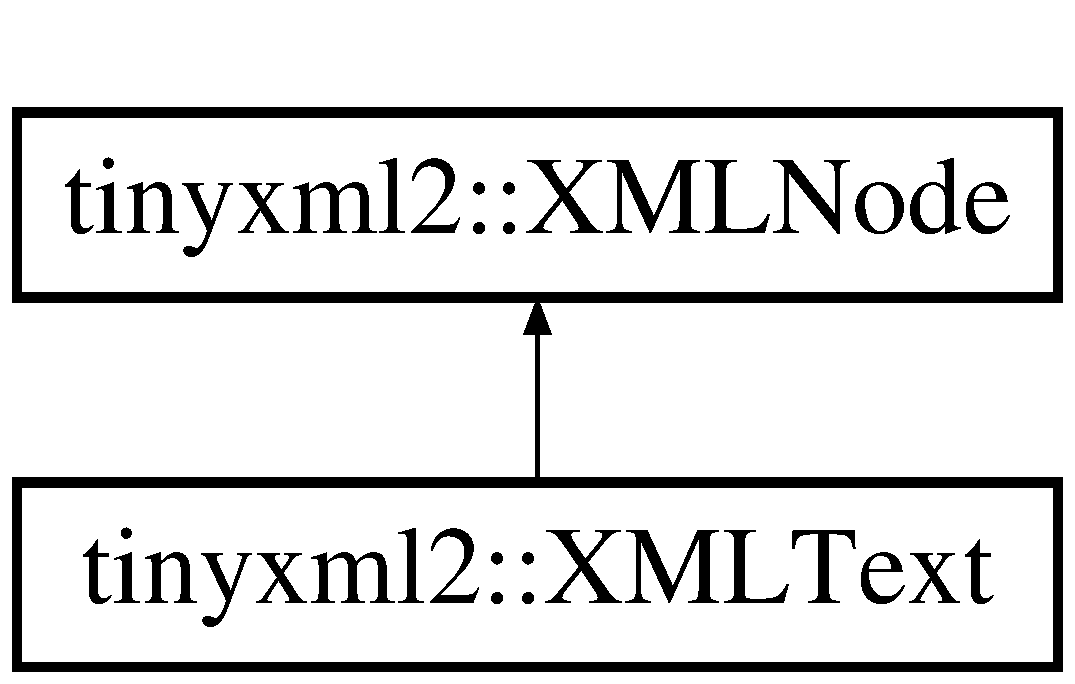
\includegraphics[height=2.000000cm]{classtinyxml2_1_1_x_m_l_text}
\end{center}
\end{figure}
\subsection*{Public Member Functions}
\begin{DoxyCompactItemize}
\item 
virtual bool \hyperlink{classtinyxml2_1_1_x_m_l_text_a537c60d7e18fb59c45ac2737a29ac47a}{Accept} (\hyperlink{classtinyxml2_1_1_x_m_l_visitor}{X\+M\+L\+Visitor} $\ast$visitor) const
\item 
virtual \hyperlink{classtinyxml2_1_1_x_m_l_text}{X\+M\+L\+Text} $\ast$ \hyperlink{classtinyxml2_1_1_x_m_l_text_ab1213b4ddebe9b17ec7e7040e9f1caf7}{To\+Text} ()
\begin{DoxyCompactList}\small\item\em Safely cast to Text, or null. \end{DoxyCompactList}\item 
virtual const \hyperlink{classtinyxml2_1_1_x_m_l_text}{X\+M\+L\+Text} $\ast$ \hyperlink{classtinyxml2_1_1_x_m_l_text_a671ce22c7c5ef378f1ce31e6f827b9e2}{To\+Text} () const
\item 
void \hyperlink{classtinyxml2_1_1_x_m_l_text_ad080357d76ab7cc59d7651249949329d}{Set\+C\+Data} (bool is\+C\+Data)
\begin{DoxyCompactList}\small\item\em Declare whether this should be C\+D\+A\+TA or standard text. \end{DoxyCompactList}\item 
bool \hyperlink{classtinyxml2_1_1_x_m_l_text_ac1bb5ea4166c320882d9e0ad16fd385b}{C\+Data} () const
\begin{DoxyCompactList}\small\item\em Returns true if this is a C\+D\+A\+TA text element. \end{DoxyCompactList}\item 
virtual \hyperlink{classtinyxml2_1_1_x_m_l_node}{X\+M\+L\+Node} $\ast$ \hyperlink{classtinyxml2_1_1_x_m_l_text_a86d265c93152726c8c6831e9594840e6}{Shallow\+Clone} (\hyperlink{classtinyxml2_1_1_x_m_l_document}{X\+M\+L\+Document} $\ast$document) const
\item 
virtual bool \hyperlink{classtinyxml2_1_1_x_m_l_text_a99d8bce4dc01df889126e047f358cdfc}{Shallow\+Equal} (const \hyperlink{classtinyxml2_1_1_x_m_l_node}{X\+M\+L\+Node} $\ast$compare) const
\end{DoxyCompactItemize}
\subsection*{Protected Member Functions}
\begin{DoxyCompactItemize}
\item 
\hyperlink{classtinyxml2_1_1_x_m_l_text_ad9f46d70e61e5386ead93728d8b90267}{X\+M\+L\+Text} (\hyperlink{classtinyxml2_1_1_x_m_l_document}{X\+M\+L\+Document} $\ast$doc)
\item 
virtual \hyperlink{classtinyxml2_1_1_x_m_l_text_ae9b8790d0dc13914394dbd7437c0e59d}{$\sim$\+X\+M\+L\+Text} ()
\item 
char $\ast$ \hyperlink{classtinyxml2_1_1_x_m_l_text_a9810dd9b82c9020baa0c3bdcb4469aac}{Parse\+Deep} (char $\ast$, \hyperlink{classtinyxml2_1_1_str_pair}{Str\+Pair} $\ast$end\+Tag, int $\ast$cur\+Line\+Num\+Ptr)
\end{DoxyCompactItemize}
\subsection*{Friends}
\begin{DoxyCompactItemize}
\item 
class \hyperlink{classtinyxml2_1_1_x_m_l_text_a4eee3bda60c60a30e4e8cd4ea91c4c6e}{X\+M\+L\+Document}
\end{DoxyCompactItemize}
\subsection*{Additional Inherited Members}


\subsection{Detailed Description}
X\+ML text.

Note that a text node can have child element nodes, for example\+: \begin{DoxyVerb}<root>This is <b>bold</b></root>
\end{DoxyVerb}


A text node can have 2 ways to output the next. \char`\"{}normal\char`\"{} output and C\+D\+A\+TA. It will default to the mode it was parsed from the X\+ML file and you generally want to leave it alone, but you can change the output mode with \hyperlink{classtinyxml2_1_1_x_m_l_text_ad080357d76ab7cc59d7651249949329d}{Set\+C\+Data()} and query it with \hyperlink{classtinyxml2_1_1_x_m_l_text_ac1bb5ea4166c320882d9e0ad16fd385b}{C\+Data()}. 

\subsection{Constructor \& Destructor Documentation}
\mbox{\Hypertarget{classtinyxml2_1_1_x_m_l_text_ad9f46d70e61e5386ead93728d8b90267}\label{classtinyxml2_1_1_x_m_l_text_ad9f46d70e61e5386ead93728d8b90267}} 
\index{tinyxml2\+::\+X\+M\+L\+Text@{tinyxml2\+::\+X\+M\+L\+Text}!X\+M\+L\+Text@{X\+M\+L\+Text}}
\index{X\+M\+L\+Text@{X\+M\+L\+Text}!tinyxml2\+::\+X\+M\+L\+Text@{tinyxml2\+::\+X\+M\+L\+Text}}
\subsubsection{\texorpdfstring{X\+M\+L\+Text()}{XMLText()}}
{\footnotesize\ttfamily tinyxml2\+::\+X\+M\+L\+Text\+::\+X\+M\+L\+Text (\begin{DoxyParamCaption}\item[{\hyperlink{classtinyxml2_1_1_x_m_l_document}{X\+M\+L\+Document} $\ast$}]{doc }\end{DoxyParamCaption})\hspace{0.3cm}{\ttfamily [inline]}, {\ttfamily [protected]}}

\mbox{\Hypertarget{classtinyxml2_1_1_x_m_l_text_ae9b8790d0dc13914394dbd7437c0e59d}\label{classtinyxml2_1_1_x_m_l_text_ae9b8790d0dc13914394dbd7437c0e59d}} 
\index{tinyxml2\+::\+X\+M\+L\+Text@{tinyxml2\+::\+X\+M\+L\+Text}!````~X\+M\+L\+Text@{$\sim$\+X\+M\+L\+Text}}
\index{````~X\+M\+L\+Text@{$\sim$\+X\+M\+L\+Text}!tinyxml2\+::\+X\+M\+L\+Text@{tinyxml2\+::\+X\+M\+L\+Text}}
\subsubsection{\texorpdfstring{$\sim$\+X\+M\+L\+Text()}{~XMLText()}}
{\footnotesize\ttfamily virtual tinyxml2\+::\+X\+M\+L\+Text\+::$\sim$\+X\+M\+L\+Text (\begin{DoxyParamCaption}{ }\end{DoxyParamCaption})\hspace{0.3cm}{\ttfamily [inline]}, {\ttfamily [protected]}, {\ttfamily [virtual]}}



\subsection{Member Function Documentation}
\mbox{\Hypertarget{classtinyxml2_1_1_x_m_l_text_a537c60d7e18fb59c45ac2737a29ac47a}\label{classtinyxml2_1_1_x_m_l_text_a537c60d7e18fb59c45ac2737a29ac47a}} 
\index{tinyxml2\+::\+X\+M\+L\+Text@{tinyxml2\+::\+X\+M\+L\+Text}!Accept@{Accept}}
\index{Accept@{Accept}!tinyxml2\+::\+X\+M\+L\+Text@{tinyxml2\+::\+X\+M\+L\+Text}}
\subsubsection{\texorpdfstring{Accept()}{Accept()}}
{\footnotesize\ttfamily bool tinyxml2\+::\+X\+M\+L\+Text\+::\+Accept (\begin{DoxyParamCaption}\item[{\hyperlink{classtinyxml2_1_1_x_m_l_visitor}{X\+M\+L\+Visitor} $\ast$}]{visitor }\end{DoxyParamCaption}) const\hspace{0.3cm}{\ttfamily [virtual]}}

Accept a hierarchical visit of the nodes in the Tiny\+X\+M\+L-\/2 D\+OM. Every node in the X\+ML tree will be conditionally visited and the host will be called back via the \hyperlink{classtinyxml2_1_1_x_m_l_visitor}{X\+M\+L\+Visitor} interface.

This is essentially a S\+AX interface for Tiny\+X\+M\+L-\/2. (Note however it doesn\textquotesingle{}t re-\/parse the X\+ML for the callbacks, so the performance of Tiny\+X\+M\+L-\/2 is unchanged by using this interface versus any other.)

The interface has been based on ideas from\+:


\begin{DoxyItemize}
\item \href{http://www.saxproject.org/}{\tt http\+://www.\+saxproject.\+org/}
\item \href{http://c2.com/cgi/wiki?HierarchicalVisitorPattern}{\tt http\+://c2.\+com/cgi/wiki?\+Hierarchical\+Visitor\+Pattern}
\end{DoxyItemize}

Which are both good references for \char`\"{}visiting\char`\"{}.

An example of using \hyperlink{classtinyxml2_1_1_x_m_l_text_a537c60d7e18fb59c45ac2737a29ac47a}{Accept()}\+: \begin{DoxyVerb}XMLPrinter printer;
tinyxmlDoc.Accept( &printer );
const char* xmlcstr = printer.CStr();
\end{DoxyVerb}
 

Implements \hyperlink{classtinyxml2_1_1_x_m_l_node_a81e66df0a44c67a7af17f3b77a152785}{tinyxml2\+::\+X\+M\+L\+Node}.

\mbox{\Hypertarget{classtinyxml2_1_1_x_m_l_text_ac1bb5ea4166c320882d9e0ad16fd385b}\label{classtinyxml2_1_1_x_m_l_text_ac1bb5ea4166c320882d9e0ad16fd385b}} 
\index{tinyxml2\+::\+X\+M\+L\+Text@{tinyxml2\+::\+X\+M\+L\+Text}!C\+Data@{C\+Data}}
\index{C\+Data@{C\+Data}!tinyxml2\+::\+X\+M\+L\+Text@{tinyxml2\+::\+X\+M\+L\+Text}}
\subsubsection{\texorpdfstring{C\+Data()}{CData()}}
{\footnotesize\ttfamily bool tinyxml2\+::\+X\+M\+L\+Text\+::\+C\+Data (\begin{DoxyParamCaption}{ }\end{DoxyParamCaption}) const\hspace{0.3cm}{\ttfamily [inline]}}



Returns true if this is a C\+D\+A\+TA text element. 

\mbox{\Hypertarget{classtinyxml2_1_1_x_m_l_text_a9810dd9b82c9020baa0c3bdcb4469aac}\label{classtinyxml2_1_1_x_m_l_text_a9810dd9b82c9020baa0c3bdcb4469aac}} 
\index{tinyxml2\+::\+X\+M\+L\+Text@{tinyxml2\+::\+X\+M\+L\+Text}!Parse\+Deep@{Parse\+Deep}}
\index{Parse\+Deep@{Parse\+Deep}!tinyxml2\+::\+X\+M\+L\+Text@{tinyxml2\+::\+X\+M\+L\+Text}}
\subsubsection{\texorpdfstring{Parse\+Deep()}{ParseDeep()}}
{\footnotesize\ttfamily char $\ast$ tinyxml2\+::\+X\+M\+L\+Text\+::\+Parse\+Deep (\begin{DoxyParamCaption}\item[{char $\ast$}]{p,  }\item[{\hyperlink{classtinyxml2_1_1_str_pair}{Str\+Pair} $\ast$}]{end\+Tag,  }\item[{int $\ast$}]{cur\+Line\+Num\+Ptr }\end{DoxyParamCaption})\hspace{0.3cm}{\ttfamily [protected]}, {\ttfamily [virtual]}}



Reimplemented from \hyperlink{classtinyxml2_1_1_x_m_l_node_a0afc27892998f31735f6225edb40a40d}{tinyxml2\+::\+X\+M\+L\+Node}.

\mbox{\Hypertarget{classtinyxml2_1_1_x_m_l_text_ad080357d76ab7cc59d7651249949329d}\label{classtinyxml2_1_1_x_m_l_text_ad080357d76ab7cc59d7651249949329d}} 
\index{tinyxml2\+::\+X\+M\+L\+Text@{tinyxml2\+::\+X\+M\+L\+Text}!Set\+C\+Data@{Set\+C\+Data}}
\index{Set\+C\+Data@{Set\+C\+Data}!tinyxml2\+::\+X\+M\+L\+Text@{tinyxml2\+::\+X\+M\+L\+Text}}
\subsubsection{\texorpdfstring{Set\+C\+Data()}{SetCData()}}
{\footnotesize\ttfamily void tinyxml2\+::\+X\+M\+L\+Text\+::\+Set\+C\+Data (\begin{DoxyParamCaption}\item[{bool}]{is\+C\+Data }\end{DoxyParamCaption})\hspace{0.3cm}{\ttfamily [inline]}}



Declare whether this should be C\+D\+A\+TA or standard text. 

\mbox{\Hypertarget{classtinyxml2_1_1_x_m_l_text_a86d265c93152726c8c6831e9594840e6}\label{classtinyxml2_1_1_x_m_l_text_a86d265c93152726c8c6831e9594840e6}} 
\index{tinyxml2\+::\+X\+M\+L\+Text@{tinyxml2\+::\+X\+M\+L\+Text}!Shallow\+Clone@{Shallow\+Clone}}
\index{Shallow\+Clone@{Shallow\+Clone}!tinyxml2\+::\+X\+M\+L\+Text@{tinyxml2\+::\+X\+M\+L\+Text}}
\subsubsection{\texorpdfstring{Shallow\+Clone()}{ShallowClone()}}
{\footnotesize\ttfamily \hyperlink{classtinyxml2_1_1_x_m_l_node}{X\+M\+L\+Node} $\ast$ tinyxml2\+::\+X\+M\+L\+Text\+::\+Shallow\+Clone (\begin{DoxyParamCaption}\item[{\hyperlink{classtinyxml2_1_1_x_m_l_document}{X\+M\+L\+Document} $\ast$}]{document }\end{DoxyParamCaption}) const\hspace{0.3cm}{\ttfamily [virtual]}}

Make a copy of this node, but not its children. You may pass in a Document pointer that will be the owner of the new Node. If the \textquotesingle{}document\textquotesingle{} is null, then the node returned will be allocated from the current Document. (this-\/$>$\hyperlink{classtinyxml2_1_1_x_m_l_node_af343d1ef0b45c0020e62d784d7e67a68}{Get\+Document()})

Note\+: if called on a \hyperlink{classtinyxml2_1_1_x_m_l_document}{X\+M\+L\+Document}, this will return null. 

Implements \hyperlink{classtinyxml2_1_1_x_m_l_node_a8402cbd3129d20e9e6024bbcc0531283}{tinyxml2\+::\+X\+M\+L\+Node}.

\mbox{\Hypertarget{classtinyxml2_1_1_x_m_l_text_a99d8bce4dc01df889126e047f358cdfc}\label{classtinyxml2_1_1_x_m_l_text_a99d8bce4dc01df889126e047f358cdfc}} 
\index{tinyxml2\+::\+X\+M\+L\+Text@{tinyxml2\+::\+X\+M\+L\+Text}!Shallow\+Equal@{Shallow\+Equal}}
\index{Shallow\+Equal@{Shallow\+Equal}!tinyxml2\+::\+X\+M\+L\+Text@{tinyxml2\+::\+X\+M\+L\+Text}}
\subsubsection{\texorpdfstring{Shallow\+Equal()}{ShallowEqual()}}
{\footnotesize\ttfamily bool tinyxml2\+::\+X\+M\+L\+Text\+::\+Shallow\+Equal (\begin{DoxyParamCaption}\item[{const \hyperlink{classtinyxml2_1_1_x_m_l_node}{X\+M\+L\+Node} $\ast$}]{compare }\end{DoxyParamCaption}) const\hspace{0.3cm}{\ttfamily [virtual]}}

Test if 2 nodes are the same, but don\textquotesingle{}t test children. The 2 nodes do not need to be in the same Document.

Note\+: if called on a \hyperlink{classtinyxml2_1_1_x_m_l_document}{X\+M\+L\+Document}, this will return false. 

Implements \hyperlink{classtinyxml2_1_1_x_m_l_node_a7ce18b751c3ea09eac292dca264f9226}{tinyxml2\+::\+X\+M\+L\+Node}.

\mbox{\Hypertarget{classtinyxml2_1_1_x_m_l_text_ab1213b4ddebe9b17ec7e7040e9f1caf7}\label{classtinyxml2_1_1_x_m_l_text_ab1213b4ddebe9b17ec7e7040e9f1caf7}} 
\index{tinyxml2\+::\+X\+M\+L\+Text@{tinyxml2\+::\+X\+M\+L\+Text}!To\+Text@{To\+Text}}
\index{To\+Text@{To\+Text}!tinyxml2\+::\+X\+M\+L\+Text@{tinyxml2\+::\+X\+M\+L\+Text}}
\subsubsection{\texorpdfstring{To\+Text()}{ToText()}\hspace{0.1cm}{\footnotesize\ttfamily [1/2]}}
{\footnotesize\ttfamily virtual \hyperlink{classtinyxml2_1_1_x_m_l_text}{X\+M\+L\+Text}$\ast$ tinyxml2\+::\+X\+M\+L\+Text\+::\+To\+Text (\begin{DoxyParamCaption}{ }\end{DoxyParamCaption})\hspace{0.3cm}{\ttfamily [inline]}, {\ttfamily [virtual]}}



Safely cast to Text, or null. 



Reimplemented from \hyperlink{classtinyxml2_1_1_x_m_l_node_a41c55dab9162d1eb62db2008430e376b}{tinyxml2\+::\+X\+M\+L\+Node}.

\mbox{\Hypertarget{classtinyxml2_1_1_x_m_l_text_a671ce22c7c5ef378f1ce31e6f827b9e2}\label{classtinyxml2_1_1_x_m_l_text_a671ce22c7c5ef378f1ce31e6f827b9e2}} 
\index{tinyxml2\+::\+X\+M\+L\+Text@{tinyxml2\+::\+X\+M\+L\+Text}!To\+Text@{To\+Text}}
\index{To\+Text@{To\+Text}!tinyxml2\+::\+X\+M\+L\+Text@{tinyxml2\+::\+X\+M\+L\+Text}}
\subsubsection{\texorpdfstring{To\+Text()}{ToText()}\hspace{0.1cm}{\footnotesize\ttfamily [2/2]}}
{\footnotesize\ttfamily virtual const \hyperlink{classtinyxml2_1_1_x_m_l_text}{X\+M\+L\+Text}$\ast$ tinyxml2\+::\+X\+M\+L\+Text\+::\+To\+Text (\begin{DoxyParamCaption}{ }\end{DoxyParamCaption}) const\hspace{0.3cm}{\ttfamily [inline]}, {\ttfamily [virtual]}}



Reimplemented from \hyperlink{classtinyxml2_1_1_x_m_l_node_acb9ccc1beda27c0efcb0545683c3e7f4}{tinyxml2\+::\+X\+M\+L\+Node}.



\subsection{Friends And Related Function Documentation}
\mbox{\Hypertarget{classtinyxml2_1_1_x_m_l_text_a4eee3bda60c60a30e4e8cd4ea91c4c6e}\label{classtinyxml2_1_1_x_m_l_text_a4eee3bda60c60a30e4e8cd4ea91c4c6e}} 
\index{tinyxml2\+::\+X\+M\+L\+Text@{tinyxml2\+::\+X\+M\+L\+Text}!X\+M\+L\+Document@{X\+M\+L\+Document}}
\index{X\+M\+L\+Document@{X\+M\+L\+Document}!tinyxml2\+::\+X\+M\+L\+Text@{tinyxml2\+::\+X\+M\+L\+Text}}
\subsubsection{\texorpdfstring{X\+M\+L\+Document}{XMLDocument}}
{\footnotesize\ttfamily friend class \hyperlink{classtinyxml2_1_1_x_m_l_document}{X\+M\+L\+Document}\hspace{0.3cm}{\ttfamily [friend]}}



The documentation for this class was generated from the following files\+:\begin{DoxyCompactItemize}
\item 
\hyperlink{tinyxml2_8h}{tinyxml2.\+h}\item 
\hyperlink{tinyxml2_8cpp}{tinyxml2.\+cpp}\end{DoxyCompactItemize}

\hypertarget{classtinyxml2_1_1_x_m_l_unknown}{}\section{tinyxml2\+:\+:X\+M\+L\+Unknown Class Reference}
\label{classtinyxml2_1_1_x_m_l_unknown}\index{tinyxml2\+::\+X\+M\+L\+Unknown@{tinyxml2\+::\+X\+M\+L\+Unknown}}


{\ttfamily \#include $<$tinyxml2.\+h$>$}

Inheritance diagram for tinyxml2\+:\+:X\+M\+L\+Unknown\+:\begin{figure}[H]
\begin{center}
\leavevmode
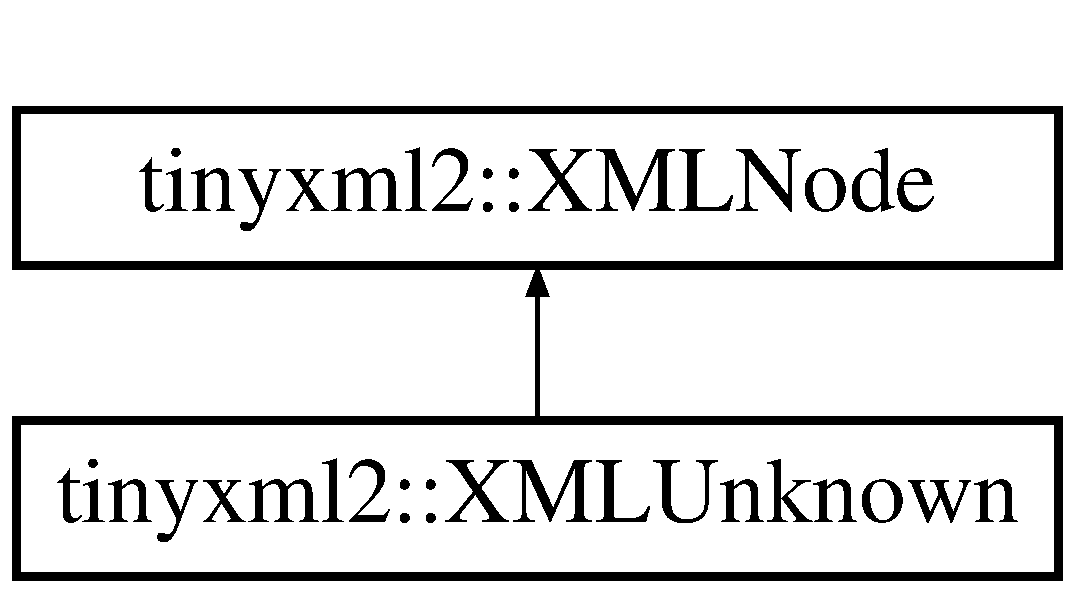
\includegraphics[height=2.000000cm]{classtinyxml2_1_1_x_m_l_unknown}
\end{center}
\end{figure}
\subsection*{Public Member Functions}
\begin{DoxyCompactItemize}
\item 
virtual \hyperlink{classtinyxml2_1_1_x_m_l_unknown}{X\+M\+L\+Unknown} $\ast$ \hyperlink{classtinyxml2_1_1_x_m_l_unknown_af4374856421921cad578c8affae872b6}{To\+Unknown} ()
\begin{DoxyCompactList}\small\item\em Safely cast to an Unknown, or null. \end{DoxyCompactList}\item 
virtual const \hyperlink{classtinyxml2_1_1_x_m_l_unknown}{X\+M\+L\+Unknown} $\ast$ \hyperlink{classtinyxml2_1_1_x_m_l_unknown_a61b342b4f295cded1dc2f4402e97f07e}{To\+Unknown} () const
\item 
virtual bool \hyperlink{classtinyxml2_1_1_x_m_l_unknown_a8a06b8c82117ca969a432e17a46830fc}{Accept} (\hyperlink{classtinyxml2_1_1_x_m_l_visitor}{X\+M\+L\+Visitor} $\ast$visitor) const
\item 
virtual \hyperlink{classtinyxml2_1_1_x_m_l_node}{X\+M\+L\+Node} $\ast$ \hyperlink{classtinyxml2_1_1_x_m_l_unknown_ab73b48b819aa4b2ef3815dc2d7d20d5f}{Shallow\+Clone} (\hyperlink{classtinyxml2_1_1_x_m_l_document}{X\+M\+L\+Document} $\ast$document) const
\item 
virtual bool \hyperlink{classtinyxml2_1_1_x_m_l_unknown_ac46767cd721d666e690a6231dfb618d1}{Shallow\+Equal} (const \hyperlink{classtinyxml2_1_1_x_m_l_node}{X\+M\+L\+Node} $\ast$compare) const
\end{DoxyCompactItemize}
\subsection*{Protected Member Functions}
\begin{DoxyCompactItemize}
\item 
\hyperlink{classtinyxml2_1_1_x_m_l_unknown_a9391eb679598d50baba424e6f1aa367b}{X\+M\+L\+Unknown} (\hyperlink{classtinyxml2_1_1_x_m_l_document}{X\+M\+L\+Document} $\ast$doc)
\item 
virtual \hyperlink{classtinyxml2_1_1_x_m_l_unknown_a86fcd722ca173a7f385bafafa879f26e}{$\sim$\+X\+M\+L\+Unknown} ()
\item 
char $\ast$ \hyperlink{classtinyxml2_1_1_x_m_l_unknown_a1101aca8aad424c131e34eb4f1289592}{Parse\+Deep} (char $\ast$, \hyperlink{classtinyxml2_1_1_str_pair}{Str\+Pair} $\ast$end\+Tag, int $\ast$cur\+Line\+Num\+Ptr)
\end{DoxyCompactItemize}
\subsection*{Friends}
\begin{DoxyCompactItemize}
\item 
class \hyperlink{classtinyxml2_1_1_x_m_l_unknown_a4eee3bda60c60a30e4e8cd4ea91c4c6e}{X\+M\+L\+Document}
\end{DoxyCompactItemize}
\subsection*{Additional Inherited Members}


\subsection{Detailed Description}
Any tag that Tiny\+X\+M\+L-\/2 doesn\textquotesingle{}t recognize is saved as an unknown. It is a tag of text, but should not be modified. It will be written back to the X\+ML, unchanged, when the file is saved.

D\+TD tags get thrown into X\+M\+L\+Unknowns. 

\subsection{Constructor \& Destructor Documentation}
\mbox{\Hypertarget{classtinyxml2_1_1_x_m_l_unknown_a9391eb679598d50baba424e6f1aa367b}\label{classtinyxml2_1_1_x_m_l_unknown_a9391eb679598d50baba424e6f1aa367b}} 
\index{tinyxml2\+::\+X\+M\+L\+Unknown@{tinyxml2\+::\+X\+M\+L\+Unknown}!X\+M\+L\+Unknown@{X\+M\+L\+Unknown}}
\index{X\+M\+L\+Unknown@{X\+M\+L\+Unknown}!tinyxml2\+::\+X\+M\+L\+Unknown@{tinyxml2\+::\+X\+M\+L\+Unknown}}
\subsubsection{\texorpdfstring{X\+M\+L\+Unknown()}{XMLUnknown()}}
{\footnotesize\ttfamily tinyxml2\+::\+X\+M\+L\+Unknown\+::\+X\+M\+L\+Unknown (\begin{DoxyParamCaption}\item[{\hyperlink{classtinyxml2_1_1_x_m_l_document}{X\+M\+L\+Document} $\ast$}]{doc }\end{DoxyParamCaption})\hspace{0.3cm}{\ttfamily [protected]}}

\mbox{\Hypertarget{classtinyxml2_1_1_x_m_l_unknown_a86fcd722ca173a7f385bafafa879f26e}\label{classtinyxml2_1_1_x_m_l_unknown_a86fcd722ca173a7f385bafafa879f26e}} 
\index{tinyxml2\+::\+X\+M\+L\+Unknown@{tinyxml2\+::\+X\+M\+L\+Unknown}!````~X\+M\+L\+Unknown@{$\sim$\+X\+M\+L\+Unknown}}
\index{````~X\+M\+L\+Unknown@{$\sim$\+X\+M\+L\+Unknown}!tinyxml2\+::\+X\+M\+L\+Unknown@{tinyxml2\+::\+X\+M\+L\+Unknown}}
\subsubsection{\texorpdfstring{$\sim$\+X\+M\+L\+Unknown()}{~XMLUnknown()}}
{\footnotesize\ttfamily tinyxml2\+::\+X\+M\+L\+Unknown\+::$\sim$\+X\+M\+L\+Unknown (\begin{DoxyParamCaption}{ }\end{DoxyParamCaption})\hspace{0.3cm}{\ttfamily [protected]}, {\ttfamily [virtual]}}



\subsection{Member Function Documentation}
\mbox{\Hypertarget{classtinyxml2_1_1_x_m_l_unknown_a8a06b8c82117ca969a432e17a46830fc}\label{classtinyxml2_1_1_x_m_l_unknown_a8a06b8c82117ca969a432e17a46830fc}} 
\index{tinyxml2\+::\+X\+M\+L\+Unknown@{tinyxml2\+::\+X\+M\+L\+Unknown}!Accept@{Accept}}
\index{Accept@{Accept}!tinyxml2\+::\+X\+M\+L\+Unknown@{tinyxml2\+::\+X\+M\+L\+Unknown}}
\subsubsection{\texorpdfstring{Accept()}{Accept()}}
{\footnotesize\ttfamily bool tinyxml2\+::\+X\+M\+L\+Unknown\+::\+Accept (\begin{DoxyParamCaption}\item[{\hyperlink{classtinyxml2_1_1_x_m_l_visitor}{X\+M\+L\+Visitor} $\ast$}]{visitor }\end{DoxyParamCaption}) const\hspace{0.3cm}{\ttfamily [virtual]}}

Accept a hierarchical visit of the nodes in the Tiny\+X\+M\+L-\/2 D\+OM. Every node in the X\+ML tree will be conditionally visited and the host will be called back via the \hyperlink{classtinyxml2_1_1_x_m_l_visitor}{X\+M\+L\+Visitor} interface.

This is essentially a S\+AX interface for Tiny\+X\+M\+L-\/2. (Note however it doesn\textquotesingle{}t re-\/parse the X\+ML for the callbacks, so the performance of Tiny\+X\+M\+L-\/2 is unchanged by using this interface versus any other.)

The interface has been based on ideas from\+:


\begin{DoxyItemize}
\item \href{http://www.saxproject.org/}{\tt http\+://www.\+saxproject.\+org/}
\item \href{http://c2.com/cgi/wiki?HierarchicalVisitorPattern}{\tt http\+://c2.\+com/cgi/wiki?\+Hierarchical\+Visitor\+Pattern}
\end{DoxyItemize}

Which are both good references for \char`\"{}visiting\char`\"{}.

An example of using \hyperlink{classtinyxml2_1_1_x_m_l_unknown_a8a06b8c82117ca969a432e17a46830fc}{Accept()}\+: \begin{DoxyVerb}XMLPrinter printer;
tinyxmlDoc.Accept( &printer );
const char* xmlcstr = printer.CStr();
\end{DoxyVerb}
 

Implements \hyperlink{classtinyxml2_1_1_x_m_l_node_a81e66df0a44c67a7af17f3b77a152785}{tinyxml2\+::\+X\+M\+L\+Node}.

\mbox{\Hypertarget{classtinyxml2_1_1_x_m_l_unknown_a1101aca8aad424c131e34eb4f1289592}\label{classtinyxml2_1_1_x_m_l_unknown_a1101aca8aad424c131e34eb4f1289592}} 
\index{tinyxml2\+::\+X\+M\+L\+Unknown@{tinyxml2\+::\+X\+M\+L\+Unknown}!Parse\+Deep@{Parse\+Deep}}
\index{Parse\+Deep@{Parse\+Deep}!tinyxml2\+::\+X\+M\+L\+Unknown@{tinyxml2\+::\+X\+M\+L\+Unknown}}
\subsubsection{\texorpdfstring{Parse\+Deep()}{ParseDeep()}}
{\footnotesize\ttfamily char $\ast$ tinyxml2\+::\+X\+M\+L\+Unknown\+::\+Parse\+Deep (\begin{DoxyParamCaption}\item[{char $\ast$}]{p,  }\item[{\hyperlink{classtinyxml2_1_1_str_pair}{Str\+Pair} $\ast$}]{end\+Tag,  }\item[{int $\ast$}]{cur\+Line\+Num\+Ptr }\end{DoxyParamCaption})\hspace{0.3cm}{\ttfamily [protected]}, {\ttfamily [virtual]}}



Reimplemented from \hyperlink{classtinyxml2_1_1_x_m_l_node_a0afc27892998f31735f6225edb40a40d}{tinyxml2\+::\+X\+M\+L\+Node}.

\mbox{\Hypertarget{classtinyxml2_1_1_x_m_l_unknown_ab73b48b819aa4b2ef3815dc2d7d20d5f}\label{classtinyxml2_1_1_x_m_l_unknown_ab73b48b819aa4b2ef3815dc2d7d20d5f}} 
\index{tinyxml2\+::\+X\+M\+L\+Unknown@{tinyxml2\+::\+X\+M\+L\+Unknown}!Shallow\+Clone@{Shallow\+Clone}}
\index{Shallow\+Clone@{Shallow\+Clone}!tinyxml2\+::\+X\+M\+L\+Unknown@{tinyxml2\+::\+X\+M\+L\+Unknown}}
\subsubsection{\texorpdfstring{Shallow\+Clone()}{ShallowClone()}}
{\footnotesize\ttfamily \hyperlink{classtinyxml2_1_1_x_m_l_node}{X\+M\+L\+Node} $\ast$ tinyxml2\+::\+X\+M\+L\+Unknown\+::\+Shallow\+Clone (\begin{DoxyParamCaption}\item[{\hyperlink{classtinyxml2_1_1_x_m_l_document}{X\+M\+L\+Document} $\ast$}]{document }\end{DoxyParamCaption}) const\hspace{0.3cm}{\ttfamily [virtual]}}

Make a copy of this node, but not its children. You may pass in a Document pointer that will be the owner of the new Node. If the \textquotesingle{}document\textquotesingle{} is null, then the node returned will be allocated from the current Document. (this-\/$>$\hyperlink{classtinyxml2_1_1_x_m_l_node_af343d1ef0b45c0020e62d784d7e67a68}{Get\+Document()})

Note\+: if called on a \hyperlink{classtinyxml2_1_1_x_m_l_document}{X\+M\+L\+Document}, this will return null. 

Implements \hyperlink{classtinyxml2_1_1_x_m_l_node_a8402cbd3129d20e9e6024bbcc0531283}{tinyxml2\+::\+X\+M\+L\+Node}.

\mbox{\Hypertarget{classtinyxml2_1_1_x_m_l_unknown_ac46767cd721d666e690a6231dfb618d1}\label{classtinyxml2_1_1_x_m_l_unknown_ac46767cd721d666e690a6231dfb618d1}} 
\index{tinyxml2\+::\+X\+M\+L\+Unknown@{tinyxml2\+::\+X\+M\+L\+Unknown}!Shallow\+Equal@{Shallow\+Equal}}
\index{Shallow\+Equal@{Shallow\+Equal}!tinyxml2\+::\+X\+M\+L\+Unknown@{tinyxml2\+::\+X\+M\+L\+Unknown}}
\subsubsection{\texorpdfstring{Shallow\+Equal()}{ShallowEqual()}}
{\footnotesize\ttfamily bool tinyxml2\+::\+X\+M\+L\+Unknown\+::\+Shallow\+Equal (\begin{DoxyParamCaption}\item[{const \hyperlink{classtinyxml2_1_1_x_m_l_node}{X\+M\+L\+Node} $\ast$}]{compare }\end{DoxyParamCaption}) const\hspace{0.3cm}{\ttfamily [virtual]}}

Test if 2 nodes are the same, but don\textquotesingle{}t test children. The 2 nodes do not need to be in the same Document.

Note\+: if called on a \hyperlink{classtinyxml2_1_1_x_m_l_document}{X\+M\+L\+Document}, this will return false. 

Implements \hyperlink{classtinyxml2_1_1_x_m_l_node_a7ce18b751c3ea09eac292dca264f9226}{tinyxml2\+::\+X\+M\+L\+Node}.

\mbox{\Hypertarget{classtinyxml2_1_1_x_m_l_unknown_af4374856421921cad578c8affae872b6}\label{classtinyxml2_1_1_x_m_l_unknown_af4374856421921cad578c8affae872b6}} 
\index{tinyxml2\+::\+X\+M\+L\+Unknown@{tinyxml2\+::\+X\+M\+L\+Unknown}!To\+Unknown@{To\+Unknown}}
\index{To\+Unknown@{To\+Unknown}!tinyxml2\+::\+X\+M\+L\+Unknown@{tinyxml2\+::\+X\+M\+L\+Unknown}}
\subsubsection{\texorpdfstring{To\+Unknown()}{ToUnknown()}\hspace{0.1cm}{\footnotesize\ttfamily [1/2]}}
{\footnotesize\ttfamily virtual \hyperlink{classtinyxml2_1_1_x_m_l_unknown}{X\+M\+L\+Unknown}$\ast$ tinyxml2\+::\+X\+M\+L\+Unknown\+::\+To\+Unknown (\begin{DoxyParamCaption}{ }\end{DoxyParamCaption})\hspace{0.3cm}{\ttfamily [inline]}, {\ttfamily [virtual]}}



Safely cast to an Unknown, or null. 



Reimplemented from \hyperlink{classtinyxml2_1_1_x_m_l_node_a8675a74aa0ada6eccab0c77ef3e5b9bd}{tinyxml2\+::\+X\+M\+L\+Node}.

\mbox{\Hypertarget{classtinyxml2_1_1_x_m_l_unknown_a61b342b4f295cded1dc2f4402e97f07e}\label{classtinyxml2_1_1_x_m_l_unknown_a61b342b4f295cded1dc2f4402e97f07e}} 
\index{tinyxml2\+::\+X\+M\+L\+Unknown@{tinyxml2\+::\+X\+M\+L\+Unknown}!To\+Unknown@{To\+Unknown}}
\index{To\+Unknown@{To\+Unknown}!tinyxml2\+::\+X\+M\+L\+Unknown@{tinyxml2\+::\+X\+M\+L\+Unknown}}
\subsubsection{\texorpdfstring{To\+Unknown()}{ToUnknown()}\hspace{0.1cm}{\footnotesize\ttfamily [2/2]}}
{\footnotesize\ttfamily virtual const \hyperlink{classtinyxml2_1_1_x_m_l_unknown}{X\+M\+L\+Unknown}$\ast$ tinyxml2\+::\+X\+M\+L\+Unknown\+::\+To\+Unknown (\begin{DoxyParamCaption}{ }\end{DoxyParamCaption}) const\hspace{0.3cm}{\ttfamily [inline]}, {\ttfamily [virtual]}}



Reimplemented from \hyperlink{classtinyxml2_1_1_x_m_l_node_af29ffd6cbe609b6fa04a705256150408}{tinyxml2\+::\+X\+M\+L\+Node}.



\subsection{Friends And Related Function Documentation}
\mbox{\Hypertarget{classtinyxml2_1_1_x_m_l_unknown_a4eee3bda60c60a30e4e8cd4ea91c4c6e}\label{classtinyxml2_1_1_x_m_l_unknown_a4eee3bda60c60a30e4e8cd4ea91c4c6e}} 
\index{tinyxml2\+::\+X\+M\+L\+Unknown@{tinyxml2\+::\+X\+M\+L\+Unknown}!X\+M\+L\+Document@{X\+M\+L\+Document}}
\index{X\+M\+L\+Document@{X\+M\+L\+Document}!tinyxml2\+::\+X\+M\+L\+Unknown@{tinyxml2\+::\+X\+M\+L\+Unknown}}
\subsubsection{\texorpdfstring{X\+M\+L\+Document}{XMLDocument}}
{\footnotesize\ttfamily friend class \hyperlink{classtinyxml2_1_1_x_m_l_document}{X\+M\+L\+Document}\hspace{0.3cm}{\ttfamily [friend]}}



The documentation for this class was generated from the following files\+:\begin{DoxyCompactItemize}
\item 
\hyperlink{tinyxml2_8h}{tinyxml2.\+h}\item 
\hyperlink{tinyxml2_8cpp}{tinyxml2.\+cpp}\end{DoxyCompactItemize}

\hypertarget{classtinyxml2_1_1_x_m_l_util}{}\section{tinyxml2\+:\+:X\+M\+L\+Util Class Reference}
\label{classtinyxml2_1_1_x_m_l_util}\index{tinyxml2\+::\+X\+M\+L\+Util@{tinyxml2\+::\+X\+M\+L\+Util}}


{\ttfamily \#include $<$tinyxml2.\+h$>$}

\subsection*{Static Public Member Functions}
\begin{DoxyCompactItemize}
\item 
static const char $\ast$ \hyperlink{classtinyxml2_1_1_x_m_l_util_ab626a194b3523a5ba8b9dbaa2a165202}{Skip\+White\+Space} (const char $\ast$p, int $\ast$cur\+Line\+Num\+Ptr)
\item 
static char $\ast$ \hyperlink{classtinyxml2_1_1_x_m_l_util_abb6cb3e71f88efca82cb7157367fd91e}{Skip\+White\+Space} (char $\ast$p, int $\ast$cur\+Line\+Num\+Ptr)
\item 
static bool \hyperlink{classtinyxml2_1_1_x_m_l_util_a357ec3af8fc433d19023a815f45e8e33}{Is\+White\+Space} (char p)
\item 
static bool \hyperlink{classtinyxml2_1_1_x_m_l_util_abe106a69ac4d942a4381a4d9dfd0e0bd}{Is\+Name\+Start\+Char} (unsigned char ch)
\item 
static bool \hyperlink{classtinyxml2_1_1_x_m_l_util_a04b17341538fa11752f24b4301d19485}{Is\+Name\+Char} (unsigned char ch)
\item 
static bool \hyperlink{classtinyxml2_1_1_x_m_l_util_acfcd287cacfd2533e1bc9ea4dfb56602}{String\+Equal} (const char $\ast$p, const char $\ast$q, int n\+Char=I\+N\+T\+\_\+\+M\+AX)
\item 
static bool \hyperlink{classtinyxml2_1_1_x_m_l_util_ad7fd82e0fe610d73ef7bf9f359f104a3}{Is\+U\+T\+F8\+Continuation} (char p)
\item 
static const char $\ast$ \hyperlink{classtinyxml2_1_1_x_m_l_util_ae9bcb2bc3cd6475fdc644c8c17790555}{Read\+B\+OM} (const char $\ast$p, bool $\ast$has\+B\+OM)
\item 
static const char $\ast$ \hyperlink{classtinyxml2_1_1_x_m_l_util_a5a96e5144a8d693dc4bcd783d9964648}{Get\+Character\+Ref} (const char $\ast$p, char $\ast$value, int $\ast$length)
\item 
static void \hyperlink{classtinyxml2_1_1_x_m_l_util_a31c00d5c5dfb38382de1dfcaf4be3595}{Convert\+U\+T\+F32\+To\+U\+T\+F8} (unsigned long input, char $\ast$output, int $\ast$length)
\item 
static void \hyperlink{classtinyxml2_1_1_x_m_l_util_a3cd6c703d49b9d51bdf0f4ff6aa021c7}{To\+Str} (int v, char $\ast$buffer, int buffer\+Size)
\item 
static void \hyperlink{classtinyxml2_1_1_x_m_l_util_ac00c2e52c1c36dab3ff41d86a9bf60f9}{To\+Str} (unsigned v, char $\ast$buffer, int buffer\+Size)
\item 
static void \hyperlink{classtinyxml2_1_1_x_m_l_util_adba0718527ae9e80f663a71ea325cb11}{To\+Str} (bool v, char $\ast$buffer, int buffer\+Size)
\item 
static void \hyperlink{classtinyxml2_1_1_x_m_l_util_a8957ad44fee5fa02ba52d73aad4d0a31}{To\+Str} (float v, char $\ast$buffer, int buffer\+Size)
\item 
static void \hyperlink{classtinyxml2_1_1_x_m_l_util_a1cd141e50980fcddd6bf9af5de4b1db7}{To\+Str} (double v, char $\ast$buffer, int buffer\+Size)
\item 
static void \hyperlink{classtinyxml2_1_1_x_m_l_util_a26a8cb5b833ad587b3af39469c8111de}{To\+Str} (int64\+\_\+t v, char $\ast$buffer, int buffer\+Size)
\item 
static bool \hyperlink{classtinyxml2_1_1_x_m_l_util_ad4df4023d11ee3fca9689c49b9707323}{To\+Int} (const char $\ast$str, int $\ast$value)
\item 
static bool \hyperlink{classtinyxml2_1_1_x_m_l_util_a210c8637d5eb4ce3d4625294af0efc2f}{To\+Unsigned} (const char $\ast$str, unsigned $\ast$value)
\item 
static bool \hyperlink{classtinyxml2_1_1_x_m_l_util_ae5b03e0a1ca5d42052a7ac540f7aa12a}{To\+Bool} (const char $\ast$str, bool $\ast$value)
\item 
static bool \hyperlink{classtinyxml2_1_1_x_m_l_util_a399e71edb5f29d61ea81d91ee0332bb9}{To\+Float} (const char $\ast$str, float $\ast$value)
\item 
static bool \hyperlink{classtinyxml2_1_1_x_m_l_util_ad8f75ac140fb19c1c6e164a957c4cd53}{To\+Double} (const char $\ast$str, double $\ast$value)
\item 
static bool \hyperlink{classtinyxml2_1_1_x_m_l_util_afe2ea09257431cd2b4b6d440552e4195}{To\+Int64} (const char $\ast$str, int64\+\_\+t $\ast$value)
\end{DoxyCompactItemize}


\subsection{Member Function Documentation}
\mbox{\Hypertarget{classtinyxml2_1_1_x_m_l_util_a31c00d5c5dfb38382de1dfcaf4be3595}\label{classtinyxml2_1_1_x_m_l_util_a31c00d5c5dfb38382de1dfcaf4be3595}} 
\index{tinyxml2\+::\+X\+M\+L\+Util@{tinyxml2\+::\+X\+M\+L\+Util}!Convert\+U\+T\+F32\+To\+U\+T\+F8@{Convert\+U\+T\+F32\+To\+U\+T\+F8}}
\index{Convert\+U\+T\+F32\+To\+U\+T\+F8@{Convert\+U\+T\+F32\+To\+U\+T\+F8}!tinyxml2\+::\+X\+M\+L\+Util@{tinyxml2\+::\+X\+M\+L\+Util}}
\subsubsection{\texorpdfstring{Convert\+U\+T\+F32\+To\+U\+T\+F8()}{ConvertUTF32ToUTF8()}}
{\footnotesize\ttfamily void tinyxml2\+::\+X\+M\+L\+Util\+::\+Convert\+U\+T\+F32\+To\+U\+T\+F8 (\begin{DoxyParamCaption}\item[{unsigned long}]{input,  }\item[{char $\ast$}]{output,  }\item[{int $\ast$}]{length }\end{DoxyParamCaption})\hspace{0.3cm}{\ttfamily [static]}}

\mbox{\Hypertarget{classtinyxml2_1_1_x_m_l_util_a5a96e5144a8d693dc4bcd783d9964648}\label{classtinyxml2_1_1_x_m_l_util_a5a96e5144a8d693dc4bcd783d9964648}} 
\index{tinyxml2\+::\+X\+M\+L\+Util@{tinyxml2\+::\+X\+M\+L\+Util}!Get\+Character\+Ref@{Get\+Character\+Ref}}
\index{Get\+Character\+Ref@{Get\+Character\+Ref}!tinyxml2\+::\+X\+M\+L\+Util@{tinyxml2\+::\+X\+M\+L\+Util}}
\subsubsection{\texorpdfstring{Get\+Character\+Ref()}{GetCharacterRef()}}
{\footnotesize\ttfamily const char $\ast$ tinyxml2\+::\+X\+M\+L\+Util\+::\+Get\+Character\+Ref (\begin{DoxyParamCaption}\item[{const char $\ast$}]{p,  }\item[{char $\ast$}]{value,  }\item[{int $\ast$}]{length }\end{DoxyParamCaption})\hspace{0.3cm}{\ttfamily [static]}}

\mbox{\Hypertarget{classtinyxml2_1_1_x_m_l_util_a04b17341538fa11752f24b4301d19485}\label{classtinyxml2_1_1_x_m_l_util_a04b17341538fa11752f24b4301d19485}} 
\index{tinyxml2\+::\+X\+M\+L\+Util@{tinyxml2\+::\+X\+M\+L\+Util}!Is\+Name\+Char@{Is\+Name\+Char}}
\index{Is\+Name\+Char@{Is\+Name\+Char}!tinyxml2\+::\+X\+M\+L\+Util@{tinyxml2\+::\+X\+M\+L\+Util}}
\subsubsection{\texorpdfstring{Is\+Name\+Char()}{IsNameChar()}}
{\footnotesize\ttfamily static bool tinyxml2\+::\+X\+M\+L\+Util\+::\+Is\+Name\+Char (\begin{DoxyParamCaption}\item[{unsigned char}]{ch }\end{DoxyParamCaption})\hspace{0.3cm}{\ttfamily [inline]}, {\ttfamily [static]}}

\mbox{\Hypertarget{classtinyxml2_1_1_x_m_l_util_abe106a69ac4d942a4381a4d9dfd0e0bd}\label{classtinyxml2_1_1_x_m_l_util_abe106a69ac4d942a4381a4d9dfd0e0bd}} 
\index{tinyxml2\+::\+X\+M\+L\+Util@{tinyxml2\+::\+X\+M\+L\+Util}!Is\+Name\+Start\+Char@{Is\+Name\+Start\+Char}}
\index{Is\+Name\+Start\+Char@{Is\+Name\+Start\+Char}!tinyxml2\+::\+X\+M\+L\+Util@{tinyxml2\+::\+X\+M\+L\+Util}}
\subsubsection{\texorpdfstring{Is\+Name\+Start\+Char()}{IsNameStartChar()}}
{\footnotesize\ttfamily static bool tinyxml2\+::\+X\+M\+L\+Util\+::\+Is\+Name\+Start\+Char (\begin{DoxyParamCaption}\item[{unsigned char}]{ch }\end{DoxyParamCaption})\hspace{0.3cm}{\ttfamily [inline]}, {\ttfamily [static]}}

\mbox{\Hypertarget{classtinyxml2_1_1_x_m_l_util_ad7fd82e0fe610d73ef7bf9f359f104a3}\label{classtinyxml2_1_1_x_m_l_util_ad7fd82e0fe610d73ef7bf9f359f104a3}} 
\index{tinyxml2\+::\+X\+M\+L\+Util@{tinyxml2\+::\+X\+M\+L\+Util}!Is\+U\+T\+F8\+Continuation@{Is\+U\+T\+F8\+Continuation}}
\index{Is\+U\+T\+F8\+Continuation@{Is\+U\+T\+F8\+Continuation}!tinyxml2\+::\+X\+M\+L\+Util@{tinyxml2\+::\+X\+M\+L\+Util}}
\subsubsection{\texorpdfstring{Is\+U\+T\+F8\+Continuation()}{IsUTF8Continuation()}}
{\footnotesize\ttfamily static bool tinyxml2\+::\+X\+M\+L\+Util\+::\+Is\+U\+T\+F8\+Continuation (\begin{DoxyParamCaption}\item[{char}]{p }\end{DoxyParamCaption})\hspace{0.3cm}{\ttfamily [inline]}, {\ttfamily [static]}}

\mbox{\Hypertarget{classtinyxml2_1_1_x_m_l_util_a357ec3af8fc433d19023a815f45e8e33}\label{classtinyxml2_1_1_x_m_l_util_a357ec3af8fc433d19023a815f45e8e33}} 
\index{tinyxml2\+::\+X\+M\+L\+Util@{tinyxml2\+::\+X\+M\+L\+Util}!Is\+White\+Space@{Is\+White\+Space}}
\index{Is\+White\+Space@{Is\+White\+Space}!tinyxml2\+::\+X\+M\+L\+Util@{tinyxml2\+::\+X\+M\+L\+Util}}
\subsubsection{\texorpdfstring{Is\+White\+Space()}{IsWhiteSpace()}}
{\footnotesize\ttfamily static bool tinyxml2\+::\+X\+M\+L\+Util\+::\+Is\+White\+Space (\begin{DoxyParamCaption}\item[{char}]{p }\end{DoxyParamCaption})\hspace{0.3cm}{\ttfamily [inline]}, {\ttfamily [static]}}

\mbox{\Hypertarget{classtinyxml2_1_1_x_m_l_util_ae9bcb2bc3cd6475fdc644c8c17790555}\label{classtinyxml2_1_1_x_m_l_util_ae9bcb2bc3cd6475fdc644c8c17790555}} 
\index{tinyxml2\+::\+X\+M\+L\+Util@{tinyxml2\+::\+X\+M\+L\+Util}!Read\+B\+OM@{Read\+B\+OM}}
\index{Read\+B\+OM@{Read\+B\+OM}!tinyxml2\+::\+X\+M\+L\+Util@{tinyxml2\+::\+X\+M\+L\+Util}}
\subsubsection{\texorpdfstring{Read\+B\+O\+M()}{ReadBOM()}}
{\footnotesize\ttfamily const char $\ast$ tinyxml2\+::\+X\+M\+L\+Util\+::\+Read\+B\+OM (\begin{DoxyParamCaption}\item[{const char $\ast$}]{p,  }\item[{bool $\ast$}]{has\+B\+OM }\end{DoxyParamCaption})\hspace{0.3cm}{\ttfamily [static]}}

\mbox{\Hypertarget{classtinyxml2_1_1_x_m_l_util_ab626a194b3523a5ba8b9dbaa2a165202}\label{classtinyxml2_1_1_x_m_l_util_ab626a194b3523a5ba8b9dbaa2a165202}} 
\index{tinyxml2\+::\+X\+M\+L\+Util@{tinyxml2\+::\+X\+M\+L\+Util}!Skip\+White\+Space@{Skip\+White\+Space}}
\index{Skip\+White\+Space@{Skip\+White\+Space}!tinyxml2\+::\+X\+M\+L\+Util@{tinyxml2\+::\+X\+M\+L\+Util}}
\subsubsection{\texorpdfstring{Skip\+White\+Space()}{SkipWhiteSpace()}\hspace{0.1cm}{\footnotesize\ttfamily [1/2]}}
{\footnotesize\ttfamily static const char$\ast$ tinyxml2\+::\+X\+M\+L\+Util\+::\+Skip\+White\+Space (\begin{DoxyParamCaption}\item[{const char $\ast$}]{p,  }\item[{int $\ast$}]{cur\+Line\+Num\+Ptr }\end{DoxyParamCaption})\hspace{0.3cm}{\ttfamily [inline]}, {\ttfamily [static]}}

\mbox{\Hypertarget{classtinyxml2_1_1_x_m_l_util_abb6cb3e71f88efca82cb7157367fd91e}\label{classtinyxml2_1_1_x_m_l_util_abb6cb3e71f88efca82cb7157367fd91e}} 
\index{tinyxml2\+::\+X\+M\+L\+Util@{tinyxml2\+::\+X\+M\+L\+Util}!Skip\+White\+Space@{Skip\+White\+Space}}
\index{Skip\+White\+Space@{Skip\+White\+Space}!tinyxml2\+::\+X\+M\+L\+Util@{tinyxml2\+::\+X\+M\+L\+Util}}
\subsubsection{\texorpdfstring{Skip\+White\+Space()}{SkipWhiteSpace()}\hspace{0.1cm}{\footnotesize\ttfamily [2/2]}}
{\footnotesize\ttfamily static char$\ast$ tinyxml2\+::\+X\+M\+L\+Util\+::\+Skip\+White\+Space (\begin{DoxyParamCaption}\item[{char $\ast$}]{p,  }\item[{int $\ast$}]{cur\+Line\+Num\+Ptr }\end{DoxyParamCaption})\hspace{0.3cm}{\ttfamily [inline]}, {\ttfamily [static]}}

\mbox{\Hypertarget{classtinyxml2_1_1_x_m_l_util_acfcd287cacfd2533e1bc9ea4dfb56602}\label{classtinyxml2_1_1_x_m_l_util_acfcd287cacfd2533e1bc9ea4dfb56602}} 
\index{tinyxml2\+::\+X\+M\+L\+Util@{tinyxml2\+::\+X\+M\+L\+Util}!String\+Equal@{String\+Equal}}
\index{String\+Equal@{String\+Equal}!tinyxml2\+::\+X\+M\+L\+Util@{tinyxml2\+::\+X\+M\+L\+Util}}
\subsubsection{\texorpdfstring{String\+Equal()}{StringEqual()}}
{\footnotesize\ttfamily static bool tinyxml2\+::\+X\+M\+L\+Util\+::\+String\+Equal (\begin{DoxyParamCaption}\item[{const char $\ast$}]{p,  }\item[{const char $\ast$}]{q,  }\item[{int}]{n\+Char = {\ttfamily INT\+\_\+MAX} }\end{DoxyParamCaption})\hspace{0.3cm}{\ttfamily [inline]}, {\ttfamily [static]}}

\mbox{\Hypertarget{classtinyxml2_1_1_x_m_l_util_ae5b03e0a1ca5d42052a7ac540f7aa12a}\label{classtinyxml2_1_1_x_m_l_util_ae5b03e0a1ca5d42052a7ac540f7aa12a}} 
\index{tinyxml2\+::\+X\+M\+L\+Util@{tinyxml2\+::\+X\+M\+L\+Util}!To\+Bool@{To\+Bool}}
\index{To\+Bool@{To\+Bool}!tinyxml2\+::\+X\+M\+L\+Util@{tinyxml2\+::\+X\+M\+L\+Util}}
\subsubsection{\texorpdfstring{To\+Bool()}{ToBool()}}
{\footnotesize\ttfamily bool tinyxml2\+::\+X\+M\+L\+Util\+::\+To\+Bool (\begin{DoxyParamCaption}\item[{const char $\ast$}]{str,  }\item[{bool $\ast$}]{value }\end{DoxyParamCaption})\hspace{0.3cm}{\ttfamily [static]}}

\mbox{\Hypertarget{classtinyxml2_1_1_x_m_l_util_ad8f75ac140fb19c1c6e164a957c4cd53}\label{classtinyxml2_1_1_x_m_l_util_ad8f75ac140fb19c1c6e164a957c4cd53}} 
\index{tinyxml2\+::\+X\+M\+L\+Util@{tinyxml2\+::\+X\+M\+L\+Util}!To\+Double@{To\+Double}}
\index{To\+Double@{To\+Double}!tinyxml2\+::\+X\+M\+L\+Util@{tinyxml2\+::\+X\+M\+L\+Util}}
\subsubsection{\texorpdfstring{To\+Double()}{ToDouble()}}
{\footnotesize\ttfamily bool tinyxml2\+::\+X\+M\+L\+Util\+::\+To\+Double (\begin{DoxyParamCaption}\item[{const char $\ast$}]{str,  }\item[{double $\ast$}]{value }\end{DoxyParamCaption})\hspace{0.3cm}{\ttfamily [static]}}

\mbox{\Hypertarget{classtinyxml2_1_1_x_m_l_util_a399e71edb5f29d61ea81d91ee0332bb9}\label{classtinyxml2_1_1_x_m_l_util_a399e71edb5f29d61ea81d91ee0332bb9}} 
\index{tinyxml2\+::\+X\+M\+L\+Util@{tinyxml2\+::\+X\+M\+L\+Util}!To\+Float@{To\+Float}}
\index{To\+Float@{To\+Float}!tinyxml2\+::\+X\+M\+L\+Util@{tinyxml2\+::\+X\+M\+L\+Util}}
\subsubsection{\texorpdfstring{To\+Float()}{ToFloat()}}
{\footnotesize\ttfamily bool tinyxml2\+::\+X\+M\+L\+Util\+::\+To\+Float (\begin{DoxyParamCaption}\item[{const char $\ast$}]{str,  }\item[{float $\ast$}]{value }\end{DoxyParamCaption})\hspace{0.3cm}{\ttfamily [static]}}

\mbox{\Hypertarget{classtinyxml2_1_1_x_m_l_util_ad4df4023d11ee3fca9689c49b9707323}\label{classtinyxml2_1_1_x_m_l_util_ad4df4023d11ee3fca9689c49b9707323}} 
\index{tinyxml2\+::\+X\+M\+L\+Util@{tinyxml2\+::\+X\+M\+L\+Util}!To\+Int@{To\+Int}}
\index{To\+Int@{To\+Int}!tinyxml2\+::\+X\+M\+L\+Util@{tinyxml2\+::\+X\+M\+L\+Util}}
\subsubsection{\texorpdfstring{To\+Int()}{ToInt()}}
{\footnotesize\ttfamily bool tinyxml2\+::\+X\+M\+L\+Util\+::\+To\+Int (\begin{DoxyParamCaption}\item[{const char $\ast$}]{str,  }\item[{int $\ast$}]{value }\end{DoxyParamCaption})\hspace{0.3cm}{\ttfamily [static]}}

\mbox{\Hypertarget{classtinyxml2_1_1_x_m_l_util_afe2ea09257431cd2b4b6d440552e4195}\label{classtinyxml2_1_1_x_m_l_util_afe2ea09257431cd2b4b6d440552e4195}} 
\index{tinyxml2\+::\+X\+M\+L\+Util@{tinyxml2\+::\+X\+M\+L\+Util}!To\+Int64@{To\+Int64}}
\index{To\+Int64@{To\+Int64}!tinyxml2\+::\+X\+M\+L\+Util@{tinyxml2\+::\+X\+M\+L\+Util}}
\subsubsection{\texorpdfstring{To\+Int64()}{ToInt64()}}
{\footnotesize\ttfamily bool tinyxml2\+::\+X\+M\+L\+Util\+::\+To\+Int64 (\begin{DoxyParamCaption}\item[{const char $\ast$}]{str,  }\item[{int64\+\_\+t $\ast$}]{value }\end{DoxyParamCaption})\hspace{0.3cm}{\ttfamily [static]}}

\mbox{\Hypertarget{classtinyxml2_1_1_x_m_l_util_a3cd6c703d49b9d51bdf0f4ff6aa021c7}\label{classtinyxml2_1_1_x_m_l_util_a3cd6c703d49b9d51bdf0f4ff6aa021c7}} 
\index{tinyxml2\+::\+X\+M\+L\+Util@{tinyxml2\+::\+X\+M\+L\+Util}!To\+Str@{To\+Str}}
\index{To\+Str@{To\+Str}!tinyxml2\+::\+X\+M\+L\+Util@{tinyxml2\+::\+X\+M\+L\+Util}}
\subsubsection{\texorpdfstring{To\+Str()}{ToStr()}\hspace{0.1cm}{\footnotesize\ttfamily [1/6]}}
{\footnotesize\ttfamily void tinyxml2\+::\+X\+M\+L\+Util\+::\+To\+Str (\begin{DoxyParamCaption}\item[{int}]{v,  }\item[{char $\ast$}]{buffer,  }\item[{int}]{buffer\+Size }\end{DoxyParamCaption})\hspace{0.3cm}{\ttfamily [static]}}

\mbox{\Hypertarget{classtinyxml2_1_1_x_m_l_util_ac00c2e52c1c36dab3ff41d86a9bf60f9}\label{classtinyxml2_1_1_x_m_l_util_ac00c2e52c1c36dab3ff41d86a9bf60f9}} 
\index{tinyxml2\+::\+X\+M\+L\+Util@{tinyxml2\+::\+X\+M\+L\+Util}!To\+Str@{To\+Str}}
\index{To\+Str@{To\+Str}!tinyxml2\+::\+X\+M\+L\+Util@{tinyxml2\+::\+X\+M\+L\+Util}}
\subsubsection{\texorpdfstring{To\+Str()}{ToStr()}\hspace{0.1cm}{\footnotesize\ttfamily [2/6]}}
{\footnotesize\ttfamily void tinyxml2\+::\+X\+M\+L\+Util\+::\+To\+Str (\begin{DoxyParamCaption}\item[{unsigned}]{v,  }\item[{char $\ast$}]{buffer,  }\item[{int}]{buffer\+Size }\end{DoxyParamCaption})\hspace{0.3cm}{\ttfamily [static]}}

\mbox{\Hypertarget{classtinyxml2_1_1_x_m_l_util_adba0718527ae9e80f663a71ea325cb11}\label{classtinyxml2_1_1_x_m_l_util_adba0718527ae9e80f663a71ea325cb11}} 
\index{tinyxml2\+::\+X\+M\+L\+Util@{tinyxml2\+::\+X\+M\+L\+Util}!To\+Str@{To\+Str}}
\index{To\+Str@{To\+Str}!tinyxml2\+::\+X\+M\+L\+Util@{tinyxml2\+::\+X\+M\+L\+Util}}
\subsubsection{\texorpdfstring{To\+Str()}{ToStr()}\hspace{0.1cm}{\footnotesize\ttfamily [3/6]}}
{\footnotesize\ttfamily void tinyxml2\+::\+X\+M\+L\+Util\+::\+To\+Str (\begin{DoxyParamCaption}\item[{bool}]{v,  }\item[{char $\ast$}]{buffer,  }\item[{int}]{buffer\+Size }\end{DoxyParamCaption})\hspace{0.3cm}{\ttfamily [static]}}

\mbox{\Hypertarget{classtinyxml2_1_1_x_m_l_util_a8957ad44fee5fa02ba52d73aad4d0a31}\label{classtinyxml2_1_1_x_m_l_util_a8957ad44fee5fa02ba52d73aad4d0a31}} 
\index{tinyxml2\+::\+X\+M\+L\+Util@{tinyxml2\+::\+X\+M\+L\+Util}!To\+Str@{To\+Str}}
\index{To\+Str@{To\+Str}!tinyxml2\+::\+X\+M\+L\+Util@{tinyxml2\+::\+X\+M\+L\+Util}}
\subsubsection{\texorpdfstring{To\+Str()}{ToStr()}\hspace{0.1cm}{\footnotesize\ttfamily [4/6]}}
{\footnotesize\ttfamily void tinyxml2\+::\+X\+M\+L\+Util\+::\+To\+Str (\begin{DoxyParamCaption}\item[{float}]{v,  }\item[{char $\ast$}]{buffer,  }\item[{int}]{buffer\+Size }\end{DoxyParamCaption})\hspace{0.3cm}{\ttfamily [static]}}

\mbox{\Hypertarget{classtinyxml2_1_1_x_m_l_util_a1cd141e50980fcddd6bf9af5de4b1db7}\label{classtinyxml2_1_1_x_m_l_util_a1cd141e50980fcddd6bf9af5de4b1db7}} 
\index{tinyxml2\+::\+X\+M\+L\+Util@{tinyxml2\+::\+X\+M\+L\+Util}!To\+Str@{To\+Str}}
\index{To\+Str@{To\+Str}!tinyxml2\+::\+X\+M\+L\+Util@{tinyxml2\+::\+X\+M\+L\+Util}}
\subsubsection{\texorpdfstring{To\+Str()}{ToStr()}\hspace{0.1cm}{\footnotesize\ttfamily [5/6]}}
{\footnotesize\ttfamily void tinyxml2\+::\+X\+M\+L\+Util\+::\+To\+Str (\begin{DoxyParamCaption}\item[{double}]{v,  }\item[{char $\ast$}]{buffer,  }\item[{int}]{buffer\+Size }\end{DoxyParamCaption})\hspace{0.3cm}{\ttfamily [static]}}

\mbox{\Hypertarget{classtinyxml2_1_1_x_m_l_util_a26a8cb5b833ad587b3af39469c8111de}\label{classtinyxml2_1_1_x_m_l_util_a26a8cb5b833ad587b3af39469c8111de}} 
\index{tinyxml2\+::\+X\+M\+L\+Util@{tinyxml2\+::\+X\+M\+L\+Util}!To\+Str@{To\+Str}}
\index{To\+Str@{To\+Str}!tinyxml2\+::\+X\+M\+L\+Util@{tinyxml2\+::\+X\+M\+L\+Util}}
\subsubsection{\texorpdfstring{To\+Str()}{ToStr()}\hspace{0.1cm}{\footnotesize\ttfamily [6/6]}}
{\footnotesize\ttfamily void tinyxml2\+::\+X\+M\+L\+Util\+::\+To\+Str (\begin{DoxyParamCaption}\item[{int64\+\_\+t}]{v,  }\item[{char $\ast$}]{buffer,  }\item[{int}]{buffer\+Size }\end{DoxyParamCaption})\hspace{0.3cm}{\ttfamily [static]}}

\mbox{\Hypertarget{classtinyxml2_1_1_x_m_l_util_a210c8637d5eb4ce3d4625294af0efc2f}\label{classtinyxml2_1_1_x_m_l_util_a210c8637d5eb4ce3d4625294af0efc2f}} 
\index{tinyxml2\+::\+X\+M\+L\+Util@{tinyxml2\+::\+X\+M\+L\+Util}!To\+Unsigned@{To\+Unsigned}}
\index{To\+Unsigned@{To\+Unsigned}!tinyxml2\+::\+X\+M\+L\+Util@{tinyxml2\+::\+X\+M\+L\+Util}}
\subsubsection{\texorpdfstring{To\+Unsigned()}{ToUnsigned()}}
{\footnotesize\ttfamily bool tinyxml2\+::\+X\+M\+L\+Util\+::\+To\+Unsigned (\begin{DoxyParamCaption}\item[{const char $\ast$}]{str,  }\item[{unsigned $\ast$}]{value }\end{DoxyParamCaption})\hspace{0.3cm}{\ttfamily [static]}}



The documentation for this class was generated from the following files\+:\begin{DoxyCompactItemize}
\item 
\hyperlink{tinyxml2_8h}{tinyxml2.\+h}\item 
\hyperlink{tinyxml2_8cpp}{tinyxml2.\+cpp}\end{DoxyCompactItemize}

\hypertarget{classtinyxml2_1_1_x_m_l_visitor}{}\section{tinyxml2\+:\+:X\+M\+L\+Visitor Class Reference}
\label{classtinyxml2_1_1_x_m_l_visitor}\index{tinyxml2\+::\+X\+M\+L\+Visitor@{tinyxml2\+::\+X\+M\+L\+Visitor}}


{\ttfamily \#include $<$tinyxml2.\+h$>$}

Inheritance diagram for tinyxml2\+:\+:X\+M\+L\+Visitor\+:\begin{figure}[H]
\begin{center}
\leavevmode
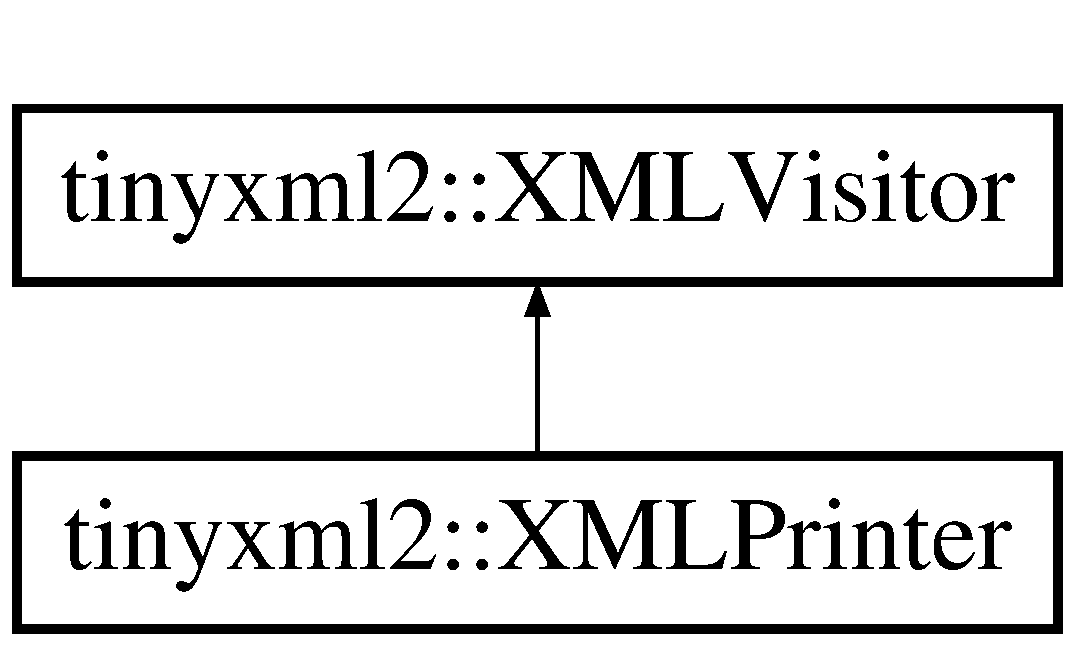
\includegraphics[height=2.000000cm]{classtinyxml2_1_1_x_m_l_visitor}
\end{center}
\end{figure}
\subsection*{Public Member Functions}
\begin{DoxyCompactItemize}
\item 
virtual \hyperlink{classtinyxml2_1_1_x_m_l_visitor_a494e72033d646c47d9c65c502ec62364}{$\sim$\+X\+M\+L\+Visitor} ()
\item 
virtual bool \hyperlink{classtinyxml2_1_1_x_m_l_visitor_acb3c22fc5f60eb9db98f533f2761f67d}{Visit\+Enter} (const \hyperlink{classtinyxml2_1_1_x_m_l_document}{X\+M\+L\+Document} \&)
\begin{DoxyCompactList}\small\item\em Visit a document. \end{DoxyCompactList}\item 
virtual bool \hyperlink{classtinyxml2_1_1_x_m_l_visitor_a170e9989cd046ba904f302d087e07086}{Visit\+Exit} (const \hyperlink{classtinyxml2_1_1_x_m_l_document}{X\+M\+L\+Document} \&)
\begin{DoxyCompactList}\small\item\em Visit a document. \end{DoxyCompactList}\item 
virtual bool \hyperlink{classtinyxml2_1_1_x_m_l_visitor_af97980a17dd4e37448b181f5ddfa92b5}{Visit\+Enter} (const \hyperlink{classtinyxml2_1_1_x_m_l_element}{X\+M\+L\+Element} \&, const \hyperlink{classtinyxml2_1_1_x_m_l_attribute}{X\+M\+L\+Attribute} $\ast$)
\begin{DoxyCompactList}\small\item\em Visit an element. \end{DoxyCompactList}\item 
virtual bool \hyperlink{classtinyxml2_1_1_x_m_l_visitor_a772f10ddc83f881956d32628faa16eb6}{Visit\+Exit} (const \hyperlink{classtinyxml2_1_1_x_m_l_element}{X\+M\+L\+Element} \&)
\begin{DoxyCompactList}\small\item\em Visit an element. \end{DoxyCompactList}\item 
virtual bool \hyperlink{classtinyxml2_1_1_x_m_l_visitor_adc75bd459fc7ba8223b50f0616767f9a}{Visit} (const \hyperlink{classtinyxml2_1_1_x_m_l_declaration}{X\+M\+L\+Declaration} \&)
\begin{DoxyCompactList}\small\item\em Visit a declaration. \end{DoxyCompactList}\item 
virtual bool \hyperlink{classtinyxml2_1_1_x_m_l_visitor_af30233565856480ea48b6fa0d6dec65b}{Visit} (const \hyperlink{classtinyxml2_1_1_x_m_l_text}{X\+M\+L\+Text} \&)
\begin{DoxyCompactList}\small\item\em Visit a text node. \end{DoxyCompactList}\item 
virtual bool \hyperlink{classtinyxml2_1_1_x_m_l_visitor_acc8147fb5a85f6c65721654e427752d7}{Visit} (const \hyperlink{classtinyxml2_1_1_x_m_l_comment}{X\+M\+L\+Comment} \&)
\begin{DoxyCompactList}\small\item\em Visit a comment node. \end{DoxyCompactList}\item 
virtual bool \hyperlink{classtinyxml2_1_1_x_m_l_visitor_a14e4748387c34bf53d24e8119bb1f292}{Visit} (const \hyperlink{classtinyxml2_1_1_x_m_l_unknown}{X\+M\+L\+Unknown} \&)
\begin{DoxyCompactList}\small\item\em Visit an unknown node. \end{DoxyCompactList}\end{DoxyCompactItemize}


\subsection{Detailed Description}
Implements the interface to the \char`\"{}\+Visitor pattern\char`\"{} (see the Accept() method.) If you call the Accept() method, it requires being passed a \hyperlink{classtinyxml2_1_1_x_m_l_visitor}{X\+M\+L\+Visitor} class to handle callbacks. For nodes that contain other nodes (Document, Element) you will get called with a Visit\+Enter/\+Visit\+Exit pair. Nodes that are always leafs are simply called with \hyperlink{classtinyxml2_1_1_x_m_l_visitor_adc75bd459fc7ba8223b50f0616767f9a}{Visit()}.

If you return \textquotesingle{}true\textquotesingle{} from a Visit method, recursive parsing will continue. If you return false, {\bfseries no children of this node or its siblings} will be visited.

All flavors of Visit methods have a default implementation that returns \textquotesingle{}true\textquotesingle{} (continue visiting). You need to only override methods that are interesting to you.

Generally Accept() is called on the \hyperlink{classtinyxml2_1_1_x_m_l_document}{X\+M\+L\+Document}, although all nodes support visiting.

You should never change the document from a callback.

\begin{DoxySeeAlso}{See also}
\hyperlink{classtinyxml2_1_1_x_m_l_node_a81e66df0a44c67a7af17f3b77a152785}{X\+M\+L\+Node\+::\+Accept()} 
\end{DoxySeeAlso}


\subsection{Constructor \& Destructor Documentation}
\mbox{\Hypertarget{classtinyxml2_1_1_x_m_l_visitor_a494e72033d646c47d9c65c502ec62364}\label{classtinyxml2_1_1_x_m_l_visitor_a494e72033d646c47d9c65c502ec62364}} 
\index{tinyxml2\+::\+X\+M\+L\+Visitor@{tinyxml2\+::\+X\+M\+L\+Visitor}!````~X\+M\+L\+Visitor@{$\sim$\+X\+M\+L\+Visitor}}
\index{````~X\+M\+L\+Visitor@{$\sim$\+X\+M\+L\+Visitor}!tinyxml2\+::\+X\+M\+L\+Visitor@{tinyxml2\+::\+X\+M\+L\+Visitor}}
\subsubsection{\texorpdfstring{$\sim$\+X\+M\+L\+Visitor()}{~XMLVisitor()}}
{\footnotesize\ttfamily virtual tinyxml2\+::\+X\+M\+L\+Visitor\+::$\sim$\+X\+M\+L\+Visitor (\begin{DoxyParamCaption}{ }\end{DoxyParamCaption})\hspace{0.3cm}{\ttfamily [inline]}, {\ttfamily [virtual]}}



\subsection{Member Function Documentation}
\mbox{\Hypertarget{classtinyxml2_1_1_x_m_l_visitor_adc75bd459fc7ba8223b50f0616767f9a}\label{classtinyxml2_1_1_x_m_l_visitor_adc75bd459fc7ba8223b50f0616767f9a}} 
\index{tinyxml2\+::\+X\+M\+L\+Visitor@{tinyxml2\+::\+X\+M\+L\+Visitor}!Visit@{Visit}}
\index{Visit@{Visit}!tinyxml2\+::\+X\+M\+L\+Visitor@{tinyxml2\+::\+X\+M\+L\+Visitor}}
\subsubsection{\texorpdfstring{Visit()}{Visit()}\hspace{0.1cm}{\footnotesize\ttfamily [1/4]}}
{\footnotesize\ttfamily virtual bool tinyxml2\+::\+X\+M\+L\+Visitor\+::\+Visit (\begin{DoxyParamCaption}\item[{const \hyperlink{classtinyxml2_1_1_x_m_l_declaration}{X\+M\+L\+Declaration} \&}]{ }\end{DoxyParamCaption})\hspace{0.3cm}{\ttfamily [inline]}, {\ttfamily [virtual]}}



Visit a declaration. 



Reimplemented in \hyperlink{classtinyxml2_1_1_x_m_l_printer_acfc625b2549304b9c7eb85ebd5c5eb39}{tinyxml2\+::\+X\+M\+L\+Printer}.

\mbox{\Hypertarget{classtinyxml2_1_1_x_m_l_visitor_af30233565856480ea48b6fa0d6dec65b}\label{classtinyxml2_1_1_x_m_l_visitor_af30233565856480ea48b6fa0d6dec65b}} 
\index{tinyxml2\+::\+X\+M\+L\+Visitor@{tinyxml2\+::\+X\+M\+L\+Visitor}!Visit@{Visit}}
\index{Visit@{Visit}!tinyxml2\+::\+X\+M\+L\+Visitor@{tinyxml2\+::\+X\+M\+L\+Visitor}}
\subsubsection{\texorpdfstring{Visit()}{Visit()}\hspace{0.1cm}{\footnotesize\ttfamily [2/4]}}
{\footnotesize\ttfamily virtual bool tinyxml2\+::\+X\+M\+L\+Visitor\+::\+Visit (\begin{DoxyParamCaption}\item[{const \hyperlink{classtinyxml2_1_1_x_m_l_text}{X\+M\+L\+Text} \&}]{ }\end{DoxyParamCaption})\hspace{0.3cm}{\ttfamily [inline]}, {\ttfamily [virtual]}}



Visit a text node. 



Reimplemented in \hyperlink{classtinyxml2_1_1_x_m_l_printer_adc0e42b4f6fcb90a95630c79575d030b}{tinyxml2\+::\+X\+M\+L\+Printer}.

\mbox{\Hypertarget{classtinyxml2_1_1_x_m_l_visitor_acc8147fb5a85f6c65721654e427752d7}\label{classtinyxml2_1_1_x_m_l_visitor_acc8147fb5a85f6c65721654e427752d7}} 
\index{tinyxml2\+::\+X\+M\+L\+Visitor@{tinyxml2\+::\+X\+M\+L\+Visitor}!Visit@{Visit}}
\index{Visit@{Visit}!tinyxml2\+::\+X\+M\+L\+Visitor@{tinyxml2\+::\+X\+M\+L\+Visitor}}
\subsubsection{\texorpdfstring{Visit()}{Visit()}\hspace{0.1cm}{\footnotesize\ttfamily [3/4]}}
{\footnotesize\ttfamily virtual bool tinyxml2\+::\+X\+M\+L\+Visitor\+::\+Visit (\begin{DoxyParamCaption}\item[{const \hyperlink{classtinyxml2_1_1_x_m_l_comment}{X\+M\+L\+Comment} \&}]{ }\end{DoxyParamCaption})\hspace{0.3cm}{\ttfamily [inline]}, {\ttfamily [virtual]}}



Visit a comment node. 



Reimplemented in \hyperlink{classtinyxml2_1_1_x_m_l_printer_aa294c5c01af0ebb9114902456e4cb53c}{tinyxml2\+::\+X\+M\+L\+Printer}.

\mbox{\Hypertarget{classtinyxml2_1_1_x_m_l_visitor_a14e4748387c34bf53d24e8119bb1f292}\label{classtinyxml2_1_1_x_m_l_visitor_a14e4748387c34bf53d24e8119bb1f292}} 
\index{tinyxml2\+::\+X\+M\+L\+Visitor@{tinyxml2\+::\+X\+M\+L\+Visitor}!Visit@{Visit}}
\index{Visit@{Visit}!tinyxml2\+::\+X\+M\+L\+Visitor@{tinyxml2\+::\+X\+M\+L\+Visitor}}
\subsubsection{\texorpdfstring{Visit()}{Visit()}\hspace{0.1cm}{\footnotesize\ttfamily [4/4]}}
{\footnotesize\ttfamily virtual bool tinyxml2\+::\+X\+M\+L\+Visitor\+::\+Visit (\begin{DoxyParamCaption}\item[{const \hyperlink{classtinyxml2_1_1_x_m_l_unknown}{X\+M\+L\+Unknown} \&}]{ }\end{DoxyParamCaption})\hspace{0.3cm}{\ttfamily [inline]}, {\ttfamily [virtual]}}



Visit an unknown node. 



Reimplemented in \hyperlink{classtinyxml2_1_1_x_m_l_printer_ab8af5455bbf9e4be2663e6642fcd7e32}{tinyxml2\+::\+X\+M\+L\+Printer}.

\mbox{\Hypertarget{classtinyxml2_1_1_x_m_l_visitor_acb3c22fc5f60eb9db98f533f2761f67d}\label{classtinyxml2_1_1_x_m_l_visitor_acb3c22fc5f60eb9db98f533f2761f67d}} 
\index{tinyxml2\+::\+X\+M\+L\+Visitor@{tinyxml2\+::\+X\+M\+L\+Visitor}!Visit\+Enter@{Visit\+Enter}}
\index{Visit\+Enter@{Visit\+Enter}!tinyxml2\+::\+X\+M\+L\+Visitor@{tinyxml2\+::\+X\+M\+L\+Visitor}}
\subsubsection{\texorpdfstring{Visit\+Enter()}{VisitEnter()}\hspace{0.1cm}{\footnotesize\ttfamily [1/2]}}
{\footnotesize\ttfamily virtual bool tinyxml2\+::\+X\+M\+L\+Visitor\+::\+Visit\+Enter (\begin{DoxyParamCaption}\item[{const \hyperlink{classtinyxml2_1_1_x_m_l_document}{X\+M\+L\+Document} \&}]{ }\end{DoxyParamCaption})\hspace{0.3cm}{\ttfamily [inline]}, {\ttfamily [virtual]}}



Visit a document. 



Reimplemented in \hyperlink{classtinyxml2_1_1_x_m_l_printer_a9aa1de11a55a07db55a90fde37d7afad}{tinyxml2\+::\+X\+M\+L\+Printer}.

\mbox{\Hypertarget{classtinyxml2_1_1_x_m_l_visitor_af97980a17dd4e37448b181f5ddfa92b5}\label{classtinyxml2_1_1_x_m_l_visitor_af97980a17dd4e37448b181f5ddfa92b5}} 
\index{tinyxml2\+::\+X\+M\+L\+Visitor@{tinyxml2\+::\+X\+M\+L\+Visitor}!Visit\+Enter@{Visit\+Enter}}
\index{Visit\+Enter@{Visit\+Enter}!tinyxml2\+::\+X\+M\+L\+Visitor@{tinyxml2\+::\+X\+M\+L\+Visitor}}
\subsubsection{\texorpdfstring{Visit\+Enter()}{VisitEnter()}\hspace{0.1cm}{\footnotesize\ttfamily [2/2]}}
{\footnotesize\ttfamily virtual bool tinyxml2\+::\+X\+M\+L\+Visitor\+::\+Visit\+Enter (\begin{DoxyParamCaption}\item[{const \hyperlink{classtinyxml2_1_1_x_m_l_element}{X\+M\+L\+Element} \&}]{,  }\item[{const \hyperlink{classtinyxml2_1_1_x_m_l_attribute}{X\+M\+L\+Attribute} $\ast$}]{ }\end{DoxyParamCaption})\hspace{0.3cm}{\ttfamily [inline]}, {\ttfamily [virtual]}}



Visit an element. 



Reimplemented in \hyperlink{classtinyxml2_1_1_x_m_l_printer_a169b2509d8eabb70811b2bb8cfd1f5d1}{tinyxml2\+::\+X\+M\+L\+Printer}.

\mbox{\Hypertarget{classtinyxml2_1_1_x_m_l_visitor_a170e9989cd046ba904f302d087e07086}\label{classtinyxml2_1_1_x_m_l_visitor_a170e9989cd046ba904f302d087e07086}} 
\index{tinyxml2\+::\+X\+M\+L\+Visitor@{tinyxml2\+::\+X\+M\+L\+Visitor}!Visit\+Exit@{Visit\+Exit}}
\index{Visit\+Exit@{Visit\+Exit}!tinyxml2\+::\+X\+M\+L\+Visitor@{tinyxml2\+::\+X\+M\+L\+Visitor}}
\subsubsection{\texorpdfstring{Visit\+Exit()}{VisitExit()}\hspace{0.1cm}{\footnotesize\ttfamily [1/2]}}
{\footnotesize\ttfamily virtual bool tinyxml2\+::\+X\+M\+L\+Visitor\+::\+Visit\+Exit (\begin{DoxyParamCaption}\item[{const \hyperlink{classtinyxml2_1_1_x_m_l_document}{X\+M\+L\+Document} \&}]{ }\end{DoxyParamCaption})\hspace{0.3cm}{\ttfamily [inline]}, {\ttfamily [virtual]}}



Visit a document. 



Reimplemented in \hyperlink{classtinyxml2_1_1_x_m_l_printer_a15fc1f2b922f540917dcf52808737b29}{tinyxml2\+::\+X\+M\+L\+Printer}.

\mbox{\Hypertarget{classtinyxml2_1_1_x_m_l_visitor_a772f10ddc83f881956d32628faa16eb6}\label{classtinyxml2_1_1_x_m_l_visitor_a772f10ddc83f881956d32628faa16eb6}} 
\index{tinyxml2\+::\+X\+M\+L\+Visitor@{tinyxml2\+::\+X\+M\+L\+Visitor}!Visit\+Exit@{Visit\+Exit}}
\index{Visit\+Exit@{Visit\+Exit}!tinyxml2\+::\+X\+M\+L\+Visitor@{tinyxml2\+::\+X\+M\+L\+Visitor}}
\subsubsection{\texorpdfstring{Visit\+Exit()}{VisitExit()}\hspace{0.1cm}{\footnotesize\ttfamily [2/2]}}
{\footnotesize\ttfamily virtual bool tinyxml2\+::\+X\+M\+L\+Visitor\+::\+Visit\+Exit (\begin{DoxyParamCaption}\item[{const \hyperlink{classtinyxml2_1_1_x_m_l_element}{X\+M\+L\+Element} \&}]{ }\end{DoxyParamCaption})\hspace{0.3cm}{\ttfamily [inline]}, {\ttfamily [virtual]}}



Visit an element. 



Reimplemented in \hyperlink{classtinyxml2_1_1_x_m_l_printer_a2edd48405971a88951c71c9df86a2f50}{tinyxml2\+::\+X\+M\+L\+Printer}.



The documentation for this class was generated from the following file\+:\begin{DoxyCompactItemize}
\item 
\hyperlink{tinyxml2_8h}{tinyxml2.\+h}\end{DoxyCompactItemize}

\chapter{File Documentation}
\hypertarget{_app_8cpp}{}\section{App.\+cpp File Reference}
\label{_app_8cpp}\index{App.\+cpp@{App.\+cpp}}
{\ttfamily \#include \char`\"{}App.\+h\char`\"{}}\newline

\hypertarget{_app_8h}{}\section{App.\+h File Reference}
\label{_app_8h}\index{App.\+h@{App.\+h}}
\subsection*{Classes}
\begin{DoxyCompactItemize}
\item 
class \hyperlink{class_app}{App}
\end{DoxyCompactItemize}

\hypertarget{_circle_8cpp}{}\section{Circle.\+cpp File Reference}
\label{_circle_8cpp}\index{Circle.\+cpp@{Circle.\+cpp}}
{\ttfamily \#include $<$math.\+h$>$}\newline
{\ttfamily \#include \char`\"{}Circle.\+h\char`\"{}}\newline

\hypertarget{_circle_8h}{}\section{Circle.\+h File Reference}
\label{_circle_8h}\index{Circle.\+h@{Circle.\+h}}
{\ttfamily \#include \char`\"{}Ideal\+Figure.\+h\char`\"{}}\newline
\subsection*{Classes}
\begin{DoxyCompactItemize}
\item 
class \hyperlink{class_circle}{Circle}
\end{DoxyCompactItemize}

\hypertarget{_convex_polygon_8cpp}{}\section{Convex\+Polygon.\+cpp File Reference}
\label{_convex_polygon_8cpp}\index{Convex\+Polygon.\+cpp@{Convex\+Polygon.\+cpp}}
{\ttfamily \#include $<$iostream$>$}\newline
{\ttfamily \#include $<$iomanip$>$}\newline
{\ttfamily \#include $<$math.\+h$>$}\newline
{\ttfamily \#include \char`\"{}Convex\+Polygon.\+h\char`\"{}}\newline
\subsection*{Functions}
\begin{DoxyCompactItemize}
\item 
double \hyperlink{_convex_polygon_8cpp_ab23e5ed6004744ceeed26a7823834fb4}{triangle\+Area} (\hyperlink{class_point}{Point} a, \hyperlink{class_point}{Point} b, \hyperlink{class_point}{Point} c)
\end{DoxyCompactItemize}


\subsection{Function Documentation}
\mbox{\Hypertarget{_convex_polygon_8cpp_ab23e5ed6004744ceeed26a7823834fb4}\label{_convex_polygon_8cpp_ab23e5ed6004744ceeed26a7823834fb4}} 
\index{Convex\+Polygon.\+cpp@{Convex\+Polygon.\+cpp}!triangle\+Area@{triangle\+Area}}
\index{triangle\+Area@{triangle\+Area}!Convex\+Polygon.\+cpp@{Convex\+Polygon.\+cpp}}
\subsubsection{\texorpdfstring{triangle\+Area()}{triangleArea()}}
{\footnotesize\ttfamily double triangle\+Area (\begin{DoxyParamCaption}\item[{\hyperlink{class_point}{Point}}]{a,  }\item[{\hyperlink{class_point}{Point}}]{b,  }\item[{\hyperlink{class_point}{Point}}]{c }\end{DoxyParamCaption})}


\hypertarget{_convex_polygon_8h}{}\section{Convex\+Polygon.\+h File Reference}
\label{_convex_polygon_8h}\index{Convex\+Polygon.\+h@{Convex\+Polygon.\+h}}
{\ttfamily \#include \char`\"{}Point\+Set.\+h\char`\"{}}\newline
{\ttfamily \#include $<$iostream$>$}\newline
\subsection*{Classes}
\begin{DoxyCompactItemize}
\item 
class \hyperlink{class_convex_polygon}{Convex\+Polygon}
\end{DoxyCompactItemize}

\hypertarget{_ellipse_8cpp}{}\section{Ellipse.\+cpp File Reference}
\label{_ellipse_8cpp}\index{Ellipse.\+cpp@{Ellipse.\+cpp}}
{\ttfamily \#include $<$math.\+h$>$}\newline
{\ttfamily \#include \char`\"{}Ellipse.\+h\char`\"{}}\newline

\hypertarget{_ellipse_8h}{}\section{Ellipse.\+h File Reference}
\label{_ellipse_8h}\index{Ellipse.\+h@{Ellipse.\+h}}
{\ttfamily \#include \char`\"{}Ideal\+Figure.\+h\char`\"{}}\newline
\subsection*{Classes}
\begin{DoxyCompactItemize}
\item 
class \hyperlink{class_ellipse}{Ellipse}
\end{DoxyCompactItemize}

\hypertarget{_figure_8cpp}{}\section{Figure.\+cpp File Reference}
\label{_figure_8cpp}\index{Figure.\+cpp@{Figure.\+cpp}}
{\ttfamily \#include $<$math.\+h$>$}\newline
{\ttfamily \#include \char`\"{}Figure.\+h\char`\"{}}\newline

\hypertarget{_figure_8h}{}\section{Figure.\+h File Reference}
\label{_figure_8h}\index{Figure.\+h@{Figure.\+h}}
{\ttfamily \#include \char`\"{}tinyxml2.\+h\char`\"{}}\newline
\subsection*{Classes}
\begin{DoxyCompactItemize}
\item 
class \hyperlink{class_point}{Point}
\item 
class \hyperlink{class_figure}{Figure}
\end{DoxyCompactItemize}

\hypertarget{_globals_8cpp}{}\section{Globals.\+cpp File Reference}
\label{_globals_8cpp}\index{Globals.\+cpp@{Globals.\+cpp}}
{\ttfamily \#include $<$iostream$>$}\newline
{\ttfamily \#include $<$conio.\+h$>$}\newline
{\ttfamily \#include $<$stdlib.\+h$>$}\newline
{\ttfamily \#include \char`\"{}Globals.\+h\char`\"{}}\newline
\subsection*{Functions}
\begin{DoxyCompactItemize}
\item 
void \hyperlink{_globals_8cpp_a6bebf1c4eb155d8589c89d709d457a5d}{Pause} (void)
\item 
void \hyperlink{_globals_8cpp_a5473c6cfd6c580642133754e141ca556}{Clear\+Screen} (void)
\end{DoxyCompactItemize}


\subsection{Function Documentation}
\mbox{\Hypertarget{_globals_8cpp_a5473c6cfd6c580642133754e141ca556}\label{_globals_8cpp_a5473c6cfd6c580642133754e141ca556}} 
\index{Globals.\+cpp@{Globals.\+cpp}!Clear\+Screen@{Clear\+Screen}}
\index{Clear\+Screen@{Clear\+Screen}!Globals.\+cpp@{Globals.\+cpp}}
\subsubsection{\texorpdfstring{Clear\+Screen()}{ClearScreen()}}
{\footnotesize\ttfamily void Clear\+Screen (\begin{DoxyParamCaption}\item[{void}]{ }\end{DoxyParamCaption})}

\mbox{\Hypertarget{_globals_8cpp_a6bebf1c4eb155d8589c89d709d457a5d}\label{_globals_8cpp_a6bebf1c4eb155d8589c89d709d457a5d}} 
\index{Globals.\+cpp@{Globals.\+cpp}!Pause@{Pause}}
\index{Pause@{Pause}!Globals.\+cpp@{Globals.\+cpp}}
\subsubsection{\texorpdfstring{Pause()}{Pause()}}
{\footnotesize\ttfamily void Pause (\begin{DoxyParamCaption}\item[{void}]{ }\end{DoxyParamCaption})}


\hypertarget{_globals_8h}{}\section{Globals.\+h File Reference}
\label{_globals_8h}\index{Globals.\+h@{Globals.\+h}}
\subsection*{Macros}
\begin{DoxyCompactItemize}
\item 
\#define \hyperlink{_globals_8h_a786e228c8f4d5c01560cd9a231df3c26}{\+\_\+app\+\_\+list\+\_\+defined\+\_\+}
\end{DoxyCompactItemize}
\subsection*{Functions}
\begin{DoxyCompactItemize}
\item 
void \hyperlink{_globals_8h_a6bebf1c4eb155d8589c89d709d457a5d}{Pause} (void)
\item 
void \hyperlink{_globals_8h_a5473c6cfd6c580642133754e141ca556}{Clear\+Screen} (void)
\end{DoxyCompactItemize}


\subsection{Macro Definition Documentation}
\mbox{\Hypertarget{_globals_8h_a786e228c8f4d5c01560cd9a231df3c26}\label{_globals_8h_a786e228c8f4d5c01560cd9a231df3c26}} 
\index{Globals.\+h@{Globals.\+h}!\+\_\+app\+\_\+list\+\_\+defined\+\_\+@{\+\_\+app\+\_\+list\+\_\+defined\+\_\+}}
\index{\+\_\+app\+\_\+list\+\_\+defined\+\_\+@{\+\_\+app\+\_\+list\+\_\+defined\+\_\+}!Globals.\+h@{Globals.\+h}}
\subsubsection{\texorpdfstring{\+\_\+app\+\_\+list\+\_\+defined\+\_\+}{\_app\_list\_defined\_}}
{\footnotesize\ttfamily \#define \+\_\+app\+\_\+list\+\_\+defined\+\_\+}



\subsection{Function Documentation}
\mbox{\Hypertarget{_globals_8h_a5473c6cfd6c580642133754e141ca556}\label{_globals_8h_a5473c6cfd6c580642133754e141ca556}} 
\index{Globals.\+h@{Globals.\+h}!Clear\+Screen@{Clear\+Screen}}
\index{Clear\+Screen@{Clear\+Screen}!Globals.\+h@{Globals.\+h}}
\subsubsection{\texorpdfstring{Clear\+Screen()}{ClearScreen()}}
{\footnotesize\ttfamily void Clear\+Screen (\begin{DoxyParamCaption}\item[{void}]{ }\end{DoxyParamCaption})}

\mbox{\Hypertarget{_globals_8h_a6bebf1c4eb155d8589c89d709d457a5d}\label{_globals_8h_a6bebf1c4eb155d8589c89d709d457a5d}} 
\index{Globals.\+h@{Globals.\+h}!Pause@{Pause}}
\index{Pause@{Pause}!Globals.\+h@{Globals.\+h}}
\subsubsection{\texorpdfstring{Pause()}{Pause()}}
{\footnotesize\ttfamily void Pause (\begin{DoxyParamCaption}\item[{void}]{ }\end{DoxyParamCaption})}


\hypertarget{_ideal_figure_8h}{}\section{Ideal\+Figure.\+h File Reference}
\label{_ideal_figure_8h}\index{Ideal\+Figure.\+h@{Ideal\+Figure.\+h}}
{\ttfamily \#include \char`\"{}Convex\+Polygon.\+h\char`\"{}}\newline
\subsection*{Classes}
\begin{DoxyCompactItemize}
\item 
class \hyperlink{class_ideal_figure}{Ideal\+Figure}
\end{DoxyCompactItemize}
\subsection*{Macros}
\begin{DoxyCompactItemize}
\item 
\#define \hyperlink{_ideal_figure_8h_a00d8c937c01b3a24f12056a00144690b}{I\+F\+\_\+\+R\+A\+S\+T\+E\+R\+\_\+\+R\+E\+Z\+O\+L\+U\+T\+I\+ON}~20
\item 
\#define \hyperlink{_ideal_figure_8h_a598a3330b3c21701223ee0ca14316eca}{PI}~3.\+1415926535897932384626433832795
\end{DoxyCompactItemize}


\subsection{Macro Definition Documentation}
\mbox{\Hypertarget{_ideal_figure_8h_a00d8c937c01b3a24f12056a00144690b}\label{_ideal_figure_8h_a00d8c937c01b3a24f12056a00144690b}} 
\index{Ideal\+Figure.\+h@{Ideal\+Figure.\+h}!I\+F\+\_\+\+R\+A\+S\+T\+E\+R\+\_\+\+R\+E\+Z\+O\+L\+U\+T\+I\+ON@{I\+F\+\_\+\+R\+A\+S\+T\+E\+R\+\_\+\+R\+E\+Z\+O\+L\+U\+T\+I\+ON}}
\index{I\+F\+\_\+\+R\+A\+S\+T\+E\+R\+\_\+\+R\+E\+Z\+O\+L\+U\+T\+I\+ON@{I\+F\+\_\+\+R\+A\+S\+T\+E\+R\+\_\+\+R\+E\+Z\+O\+L\+U\+T\+I\+ON}!Ideal\+Figure.\+h@{Ideal\+Figure.\+h}}
\subsubsection{\texorpdfstring{I\+F\+\_\+\+R\+A\+S\+T\+E\+R\+\_\+\+R\+E\+Z\+O\+L\+U\+T\+I\+ON}{IF\_RASTER\_REZOLUTION}}
{\footnotesize\ttfamily \#define I\+F\+\_\+\+R\+A\+S\+T\+E\+R\+\_\+\+R\+E\+Z\+O\+L\+U\+T\+I\+ON~20}

\mbox{\Hypertarget{_ideal_figure_8h_a598a3330b3c21701223ee0ca14316eca}\label{_ideal_figure_8h_a598a3330b3c21701223ee0ca14316eca}} 
\index{Ideal\+Figure.\+h@{Ideal\+Figure.\+h}!PI@{PI}}
\index{PI@{PI}!Ideal\+Figure.\+h@{Ideal\+Figure.\+h}}
\subsubsection{\texorpdfstring{PI}{PI}}
{\footnotesize\ttfamily \#define PI~3.\+1415926535897932384626433832795}


\hypertarget{_list_8cpp}{}\section{List.\+cpp File Reference}
\label{_list_8cpp}\index{List.\+cpp@{List.\+cpp}}

\hypertarget{_list_8h}{}\section{List.\+h File Reference}
\label{_list_8h}\index{List.\+h@{List.\+h}}
\subsection*{Classes}
\begin{DoxyCompactItemize}
\item 
class \hyperlink{class_list}{List$<$ T $>$}
\item 
struct \hyperlink{struct_list_1_1list_elem}{List$<$ T $>$\+::list\+Elem}
\end{DoxyCompactItemize}

\hypertarget{_main_8cpp}{}\section{Main.\+cpp File Reference}
\label{_main_8cpp}\index{Main.\+cpp@{Main.\+cpp}}
{\ttfamily \#include $<$iostream$>$}\newline
{\ttfamily \#include $<$fstream$>$}\newline
{\ttfamily \#include $<$stdio.\+h$>$}\newline
{\ttfamily \#include \char`\"{}App.\+h\char`\"{}}\newline
{\ttfamily \#include \char`\"{}List.\+h\char`\"{}}\newline
{\ttfamily \#include \char`\"{}Ellipse.\+h\char`\"{}}\newline
{\ttfamily \#include \char`\"{}Circle.\+h\char`\"{}}\newline
{\ttfamily \#include \char`\"{}Convex\+Polygon.\+h\char`\"{}}\newline
{\ttfamily \#include \char`\"{}tinyxml2.\+h\char`\"{}}\newline
\subsection*{Functions}
\begin{DoxyCompactItemize}
\item 
int \hyperlink{_main_8cpp_ae66f6b31b5ad750f1fe042a706a4e3d4}{main} ()
\end{DoxyCompactItemize}


\subsection{Function Documentation}
\mbox{\Hypertarget{_main_8cpp_ae66f6b31b5ad750f1fe042a706a4e3d4}\label{_main_8cpp_ae66f6b31b5ad750f1fe042a706a4e3d4}} 
\index{Main.\+cpp@{Main.\+cpp}!main@{main}}
\index{main@{main}!Main.\+cpp@{Main.\+cpp}}
\subsubsection{\texorpdfstring{main()}{main()}}
{\footnotesize\ttfamily int main (\begin{DoxyParamCaption}{ }\end{DoxyParamCaption})}


\hypertarget{_menu_8cpp}{}\section{Menu.\+cpp File Reference}
\label{_menu_8cpp}\index{Menu.\+cpp@{Menu.\+cpp}}
{\ttfamily \#include $<$iostream$>$}\newline
{\ttfamily \#include $<$conio.\+h$>$}\newline
{\ttfamily \#include $<$string.\+h$>$}\newline
{\ttfamily \#include \char`\"{}Globals.\+h\char`\"{}}\newline
{\ttfamily \#include \char`\"{}Menu.\+h\char`\"{}}\newline

\hypertarget{_menu_8h}{}\section{Menu.\+h File Reference}
\label{_menu_8h}\index{Menu.\+h@{Menu.\+h}}
\subsection*{Classes}
\begin{DoxyCompactItemize}
\item 
class \hyperlink{class_menu_item}{Menu\+Item}
\item 
class \hyperlink{class_operation}{Operation}
\item 
class \hyperlink{class_menu}{Menu}
\end{DoxyCompactItemize}

\hypertarget{_point_set_8cpp}{}\section{Point\+Set.\+cpp File Reference}
\label{_point_set_8cpp}\index{Point\+Set.\+cpp@{Point\+Set.\+cpp}}
{\ttfamily \#include \char`\"{}Point\+Set.\+h\char`\"{}}\newline

\hypertarget{_point_set_8h}{}\section{Point\+Set.\+h File Reference}
\label{_point_set_8h}\index{Point\+Set.\+h@{Point\+Set.\+h}}
{\ttfamily \#include \char`\"{}Figure.\+h\char`\"{}}\newline
{\ttfamily \#include \char`\"{}List.\+h\char`\"{}}\newline
\subsection*{Classes}
\begin{DoxyCompactItemize}
\item 
class \hyperlink{class_point_set}{Point\+Set}
\end{DoxyCompactItemize}

\hypertarget{tinyxml2_8cpp}{}\section{tinyxml2.\+cpp File Reference}
\label{tinyxml2_8cpp}\index{tinyxml2.\+cpp@{tinyxml2.\+cpp}}
{\ttfamily \#include \char`\"{}tinyxml2.\+h\char`\"{}}\newline
{\ttfamily \#include $<$new$>$}\newline
{\ttfamily \#include $<$cstddef$>$}\newline
{\ttfamily \#include $<$cstdarg$>$}\newline
\subsection*{Classes}
\begin{DoxyCompactItemize}
\item 
struct \hyperlink{structtinyxml2_1_1_entity}{tinyxml2\+::\+Entity}
\item 
struct \hyperlink{structtinyxml2_1_1_long_fits_into_size_t_minus_one}{tinyxml2\+::\+Long\+Fits\+Into\+Size\+T\+Minus\+One$<$ bool $>$}
\item 
struct \hyperlink{structtinyxml2_1_1_long_fits_into_size_t_minus_one_3_01false_01_4}{tinyxml2\+::\+Long\+Fits\+Into\+Size\+T\+Minus\+One$<$ false $>$}
\end{DoxyCompactItemize}
\subsection*{Namespaces}
\begin{DoxyCompactItemize}
\item 
 \hyperlink{namespacetinyxml2}{tinyxml2}
\end{DoxyCompactItemize}
\subsection*{Macros}
\begin{DoxyCompactItemize}
\item 
\#define \hyperlink{tinyxml2_8cpp_afc6433f9b56e4f18833089b1df629e0a}{T\+I\+X\+M\+L\+\_\+\+S\+N\+P\+R\+I\+N\+TF}~snprintf
\item 
\#define \hyperlink{tinyxml2_8cpp_a924d10d64b020e9dbcd2b8b024768608}{T\+I\+X\+M\+L\+\_\+\+V\+S\+N\+P\+R\+I\+N\+TF}~vsnprintf
\item 
\#define \hyperlink{tinyxml2_8cpp_a96f54d7c855ad92e705510904a040393}{T\+I\+X\+M\+L\+\_\+\+S\+S\+C\+A\+NF}~sscanf
\end{DoxyCompactItemize}


\subsection{Macro Definition Documentation}
\mbox{\Hypertarget{tinyxml2_8cpp_afc6433f9b56e4f18833089b1df629e0a}\label{tinyxml2_8cpp_afc6433f9b56e4f18833089b1df629e0a}} 
\index{tinyxml2.\+cpp@{tinyxml2.\+cpp}!T\+I\+X\+M\+L\+\_\+\+S\+N\+P\+R\+I\+N\+TF@{T\+I\+X\+M\+L\+\_\+\+S\+N\+P\+R\+I\+N\+TF}}
\index{T\+I\+X\+M\+L\+\_\+\+S\+N\+P\+R\+I\+N\+TF@{T\+I\+X\+M\+L\+\_\+\+S\+N\+P\+R\+I\+N\+TF}!tinyxml2.\+cpp@{tinyxml2.\+cpp}}
\subsubsection{\texorpdfstring{T\+I\+X\+M\+L\+\_\+\+S\+N\+P\+R\+I\+N\+TF}{TIXML\_SNPRINTF}}
{\footnotesize\ttfamily \#define T\+I\+X\+M\+L\+\_\+\+S\+N\+P\+R\+I\+N\+TF~snprintf}

\mbox{\Hypertarget{tinyxml2_8cpp_a96f54d7c855ad92e705510904a040393}\label{tinyxml2_8cpp_a96f54d7c855ad92e705510904a040393}} 
\index{tinyxml2.\+cpp@{tinyxml2.\+cpp}!T\+I\+X\+M\+L\+\_\+\+S\+S\+C\+A\+NF@{T\+I\+X\+M\+L\+\_\+\+S\+S\+C\+A\+NF}}
\index{T\+I\+X\+M\+L\+\_\+\+S\+S\+C\+A\+NF@{T\+I\+X\+M\+L\+\_\+\+S\+S\+C\+A\+NF}!tinyxml2.\+cpp@{tinyxml2.\+cpp}}
\subsubsection{\texorpdfstring{T\+I\+X\+M\+L\+\_\+\+S\+S\+C\+A\+NF}{TIXML\_SSCANF}}
{\footnotesize\ttfamily \#define T\+I\+X\+M\+L\+\_\+\+S\+S\+C\+A\+NF~sscanf}

\mbox{\Hypertarget{tinyxml2_8cpp_a924d10d64b020e9dbcd2b8b024768608}\label{tinyxml2_8cpp_a924d10d64b020e9dbcd2b8b024768608}} 
\index{tinyxml2.\+cpp@{tinyxml2.\+cpp}!T\+I\+X\+M\+L\+\_\+\+V\+S\+N\+P\+R\+I\+N\+TF@{T\+I\+X\+M\+L\+\_\+\+V\+S\+N\+P\+R\+I\+N\+TF}}
\index{T\+I\+X\+M\+L\+\_\+\+V\+S\+N\+P\+R\+I\+N\+TF@{T\+I\+X\+M\+L\+\_\+\+V\+S\+N\+P\+R\+I\+N\+TF}!tinyxml2.\+cpp@{tinyxml2.\+cpp}}
\subsubsection{\texorpdfstring{T\+I\+X\+M\+L\+\_\+\+V\+S\+N\+P\+R\+I\+N\+TF}{TIXML\_VSNPRINTF}}
{\footnotesize\ttfamily \#define T\+I\+X\+M\+L\+\_\+\+V\+S\+N\+P\+R\+I\+N\+TF~vsnprintf}


\hypertarget{tinyxml2_8h}{}\section{tinyxml2.\+h File Reference}
\label{tinyxml2_8h}\index{tinyxml2.\+h@{tinyxml2.\+h}}
{\ttfamily \#include $<$cctype$>$}\newline
{\ttfamily \#include $<$climits$>$}\newline
{\ttfamily \#include $<$cstdio$>$}\newline
{\ttfamily \#include $<$cstdlib$>$}\newline
{\ttfamily \#include $<$cstring$>$}\newline
{\ttfamily \#include $<$stdint.\+h$>$}\newline
\subsection*{Classes}
\begin{DoxyCompactItemize}
\item 
class \hyperlink{classtinyxml2_1_1_str_pair}{tinyxml2\+::\+Str\+Pair}
\item 
class \hyperlink{classtinyxml2_1_1_dyn_array}{tinyxml2\+::\+Dyn\+Array$<$ T, I\+N\+I\+T\+I\+A\+L\+\_\+\+S\+I\+Z\+E $>$}
\item 
class \hyperlink{classtinyxml2_1_1_mem_pool}{tinyxml2\+::\+Mem\+Pool}
\item 
class \hyperlink{classtinyxml2_1_1_mem_pool_t}{tinyxml2\+::\+Mem\+Pool\+T$<$ I\+T\+E\+M\+\_\+\+S\+I\+Z\+E $>$}
\item 
class \hyperlink{classtinyxml2_1_1_x_m_l_visitor}{tinyxml2\+::\+X\+M\+L\+Visitor}
\item 
class \hyperlink{classtinyxml2_1_1_x_m_l_util}{tinyxml2\+::\+X\+M\+L\+Util}
\item 
class \hyperlink{classtinyxml2_1_1_x_m_l_node}{tinyxml2\+::\+X\+M\+L\+Node}
\item 
class \hyperlink{classtinyxml2_1_1_x_m_l_text}{tinyxml2\+::\+X\+M\+L\+Text}
\item 
class \hyperlink{classtinyxml2_1_1_x_m_l_comment}{tinyxml2\+::\+X\+M\+L\+Comment}
\item 
class \hyperlink{classtinyxml2_1_1_x_m_l_declaration}{tinyxml2\+::\+X\+M\+L\+Declaration}
\item 
class \hyperlink{classtinyxml2_1_1_x_m_l_unknown}{tinyxml2\+::\+X\+M\+L\+Unknown}
\item 
class \hyperlink{classtinyxml2_1_1_x_m_l_attribute}{tinyxml2\+::\+X\+M\+L\+Attribute}
\item 
class \hyperlink{classtinyxml2_1_1_x_m_l_element}{tinyxml2\+::\+X\+M\+L\+Element}
\item 
class \hyperlink{classtinyxml2_1_1_x_m_l_document}{tinyxml2\+::\+X\+M\+L\+Document}
\item 
class \hyperlink{classtinyxml2_1_1_x_m_l_handle}{tinyxml2\+::\+X\+M\+L\+Handle}
\item 
class \hyperlink{classtinyxml2_1_1_x_m_l_const_handle}{tinyxml2\+::\+X\+M\+L\+Const\+Handle}
\item 
class \hyperlink{classtinyxml2_1_1_x_m_l_printer}{tinyxml2\+::\+X\+M\+L\+Printer}
\end{DoxyCompactItemize}
\subsection*{Namespaces}
\begin{DoxyCompactItemize}
\item 
 \hyperlink{namespacetinyxml2}{tinyxml2}
\end{DoxyCompactItemize}
\subsection*{Macros}
\begin{DoxyCompactItemize}
\item 
\#define \hyperlink{tinyxml2_8h_a8953517b8490d756ad0bfef40fe5811f}{T\+I\+N\+Y\+X\+M\+L2\+\_\+\+L\+IB}
\item 
\#define \hyperlink{tinyxml2_8h_a029877acb3c6fd71698561044953bd14}{T\+I\+X\+M\+L\+A\+S\+S\+E\+RT}(x)~\{\}
\end{DoxyCompactItemize}
\subsection*{Enumerations}
\begin{DoxyCompactItemize}
\item 
enum \hyperlink{namespacetinyxml2_a1fbf88509c3ac88c09117b1947414e08}{tinyxml2\+::\+X\+M\+L\+Error} \{ \newline
\hyperlink{namespacetinyxml2_a1fbf88509c3ac88c09117b1947414e08a1fe1262fdb5ac05dd9cc4631f8c8e00d}{tinyxml2\+::\+X\+M\+L\+\_\+\+S\+U\+C\+C\+E\+SS} = 0, 
\hyperlink{namespacetinyxml2_a1fbf88509c3ac88c09117b1947414e08abefb89c44285fb68e2218b2c71767f27}{tinyxml2\+::\+X\+M\+L\+\_\+\+N\+O\+\_\+\+A\+T\+T\+R\+I\+B\+U\+TE}, 
\hyperlink{namespacetinyxml2_a1fbf88509c3ac88c09117b1947414e08ae9d8ee545a3a69e90df303257a658113}{tinyxml2\+::\+X\+M\+L\+\_\+\+W\+R\+O\+N\+G\+\_\+\+A\+T\+T\+R\+I\+B\+U\+T\+E\+\_\+\+T\+Y\+PE}, 
\hyperlink{namespacetinyxml2_a1fbf88509c3ac88c09117b1947414e08a38fd2a97fb1dbebd4c3640d75dc01a94}{tinyxml2\+::\+X\+M\+L\+\_\+\+E\+R\+R\+O\+R\+\_\+\+F\+I\+L\+E\+\_\+\+N\+O\+T\+\_\+\+F\+O\+U\+ND}, 
\newline
\hyperlink{namespacetinyxml2_a1fbf88509c3ac88c09117b1947414e08afbbf37655523b79a88b04b77ec0f1258}{tinyxml2\+::\+X\+M\+L\+\_\+\+E\+R\+R\+O\+R\+\_\+\+F\+I\+L\+E\+\_\+\+C\+O\+U\+L\+D\+\_\+\+N\+O\+T\+\_\+\+B\+E\+\_\+\+O\+P\+E\+N\+ED}, 
\hyperlink{namespacetinyxml2_a1fbf88509c3ac88c09117b1947414e08a8d4dd3ce2dee784a53f62fa8a6ac83ee}{tinyxml2\+::\+X\+M\+L\+\_\+\+E\+R\+R\+O\+R\+\_\+\+F\+I\+L\+E\+\_\+\+R\+E\+A\+D\+\_\+\+E\+R\+R\+OR}, 
\hyperlink{namespacetinyxml2_a1fbf88509c3ac88c09117b1947414e08a37759723c0c5e954597654e4eccb4f4d}{tinyxml2\+::\+X\+M\+L\+\_\+\+E\+R\+R\+O\+R\+\_\+\+E\+L\+E\+M\+E\+N\+T\+\_\+\+M\+I\+S\+M\+A\+T\+CH}, 
\hyperlink{namespacetinyxml2_a1fbf88509c3ac88c09117b1947414e08afa96ea783aa93ea212f9e2d7d3a70ba5}{tinyxml2\+::\+X\+M\+L\+\_\+\+E\+R\+R\+O\+R\+\_\+\+P\+A\+R\+S\+I\+N\+G\+\_\+\+E\+L\+E\+M\+E\+NT}, 
\newline
\hyperlink{namespacetinyxml2_a1fbf88509c3ac88c09117b1947414e08a380fd8846799b88773321efae83d26a3}{tinyxml2\+::\+X\+M\+L\+\_\+\+E\+R\+R\+O\+R\+\_\+\+P\+A\+R\+S\+I\+N\+G\+\_\+\+A\+T\+T\+R\+I\+B\+U\+TE}, 
\hyperlink{namespacetinyxml2_a1fbf88509c3ac88c09117b1947414e08a48e646cfca6de90c3770faf535d3ed6b}{tinyxml2\+::\+X\+M\+L\+\_\+\+E\+R\+R\+O\+R\+\_\+\+I\+D\+E\+N\+T\+I\+F\+Y\+I\+N\+G\+\_\+\+T\+AG}, 
\hyperlink{namespacetinyxml2_a1fbf88509c3ac88c09117b1947414e08a50ead30b94c7ae2957b9ccb08ec0994d}{tinyxml2\+::\+X\+M\+L\+\_\+\+E\+R\+R\+O\+R\+\_\+\+P\+A\+R\+S\+I\+N\+G\+\_\+\+T\+E\+XT}, 
\hyperlink{namespacetinyxml2_a1fbf88509c3ac88c09117b1947414e08a9d181628a1819f2b97835e6bc2c8bb3b}{tinyxml2\+::\+X\+M\+L\+\_\+\+E\+R\+R\+O\+R\+\_\+\+P\+A\+R\+S\+I\+N\+G\+\_\+\+C\+D\+A\+TA}, 
\newline
\hyperlink{namespacetinyxml2_a1fbf88509c3ac88c09117b1947414e08a51786809e8b079c770853cf5890a7a35}{tinyxml2\+::\+X\+M\+L\+\_\+\+E\+R\+R\+O\+R\+\_\+\+P\+A\+R\+S\+I\+N\+G\+\_\+\+C\+O\+M\+M\+E\+NT}, 
\hyperlink{namespacetinyxml2_a1fbf88509c3ac88c09117b1947414e08ad45b208578e30dab5a21bff1d8991b87}{tinyxml2\+::\+X\+M\+L\+\_\+\+E\+R\+R\+O\+R\+\_\+\+P\+A\+R\+S\+I\+N\+G\+\_\+\+D\+E\+C\+L\+A\+R\+A\+T\+I\+ON}, 
\hyperlink{namespacetinyxml2_a1fbf88509c3ac88c09117b1947414e08a95a88813812a680fb7372f0149420a97}{tinyxml2\+::\+X\+M\+L\+\_\+\+E\+R\+R\+O\+R\+\_\+\+P\+A\+R\+S\+I\+N\+G\+\_\+\+U\+N\+K\+N\+O\+WN}, 
\hyperlink{namespacetinyxml2_a1fbf88509c3ac88c09117b1947414e08a1a0478cf44f0a733aa6f21bdf0db80b5}{tinyxml2\+::\+X\+M\+L\+\_\+\+E\+R\+R\+O\+R\+\_\+\+E\+M\+P\+T\+Y\+\_\+\+D\+O\+C\+U\+M\+E\+NT}, 
\newline
\hyperlink{namespacetinyxml2_a1fbf88509c3ac88c09117b1947414e08a0cecc816939d9155d33b8a88fd50e4c1}{tinyxml2\+::\+X\+M\+L\+\_\+\+E\+R\+R\+O\+R\+\_\+\+M\+I\+S\+M\+A\+T\+C\+H\+E\+D\+\_\+\+E\+L\+E\+M\+E\+NT}, 
\hyperlink{namespacetinyxml2_a1fbf88509c3ac88c09117b1947414e08af6b4caa10e1f2e9f19a3a24f5f3ce223}{tinyxml2\+::\+X\+M\+L\+\_\+\+E\+R\+R\+O\+R\+\_\+\+P\+A\+R\+S\+I\+NG}, 
\hyperlink{namespacetinyxml2_a1fbf88509c3ac88c09117b1947414e08afdb8840395a7c13dfe6a3e104401c095}{tinyxml2\+::\+X\+M\+L\+\_\+\+C\+A\+N\+\_\+\+N\+O\+T\+\_\+\+C\+O\+N\+V\+E\+R\+T\+\_\+\+T\+E\+XT}, 
\hyperlink{namespacetinyxml2_a1fbf88509c3ac88c09117b1947414e08a5300bec98feccc8f0cdf567b88821f33}{tinyxml2\+::\+X\+M\+L\+\_\+\+N\+O\+\_\+\+T\+E\+X\+T\+\_\+\+N\+O\+DE}, 
\newline
\hyperlink{namespacetinyxml2_a1fbf88509c3ac88c09117b1947414e08a9ebb2775c56387353f5b2de94f6ab71d}{tinyxml2\+::\+X\+M\+L\+\_\+\+E\+R\+R\+O\+R\+\_\+\+C\+O\+U\+NT}
 \}
\item 
enum \hyperlink{namespacetinyxml2_a7f91d00f77360f850fd5da0861e27dd5}{tinyxml2\+::\+Whitespace} \{ \hyperlink{namespacetinyxml2_a7f91d00f77360f850fd5da0861e27dd5a751769aa625fe5fe5286e9779edec56a}{tinyxml2\+::\+P\+R\+E\+S\+E\+R\+V\+E\+\_\+\+W\+H\+I\+T\+E\+S\+P\+A\+CE}, 
\hyperlink{namespacetinyxml2_a7f91d00f77360f850fd5da0861e27dd5a9a4a309029a6f5e636e20ef5e0b65136}{tinyxml2\+::\+C\+O\+L\+L\+A\+P\+S\+E\+\_\+\+W\+H\+I\+T\+E\+S\+P\+A\+CE}
 \}
\end{DoxyCompactItemize}


\subsection{Macro Definition Documentation}
\mbox{\Hypertarget{tinyxml2_8h_a8953517b8490d756ad0bfef40fe5811f}\label{tinyxml2_8h_a8953517b8490d756ad0bfef40fe5811f}} 
\index{tinyxml2.\+h@{tinyxml2.\+h}!T\+I\+N\+Y\+X\+M\+L2\+\_\+\+L\+IB@{T\+I\+N\+Y\+X\+M\+L2\+\_\+\+L\+IB}}
\index{T\+I\+N\+Y\+X\+M\+L2\+\_\+\+L\+IB@{T\+I\+N\+Y\+X\+M\+L2\+\_\+\+L\+IB}!tinyxml2.\+h@{tinyxml2.\+h}}
\subsubsection{\texorpdfstring{T\+I\+N\+Y\+X\+M\+L2\+\_\+\+L\+IB}{TINYXML2\_LIB}}
{\footnotesize\ttfamily \#define T\+I\+N\+Y\+X\+M\+L2\+\_\+\+L\+IB}

\mbox{\Hypertarget{tinyxml2_8h_a029877acb3c6fd71698561044953bd14}\label{tinyxml2_8h_a029877acb3c6fd71698561044953bd14}} 
\index{tinyxml2.\+h@{tinyxml2.\+h}!T\+I\+X\+M\+L\+A\+S\+S\+E\+RT@{T\+I\+X\+M\+L\+A\+S\+S\+E\+RT}}
\index{T\+I\+X\+M\+L\+A\+S\+S\+E\+RT@{T\+I\+X\+M\+L\+A\+S\+S\+E\+RT}!tinyxml2.\+h@{tinyxml2.\+h}}
\subsubsection{\texorpdfstring{T\+I\+X\+M\+L\+A\+S\+S\+E\+RT}{TIXMLASSERT}}
{\footnotesize\ttfamily \#define T\+I\+X\+M\+L\+A\+S\+S\+E\+RT(\begin{DoxyParamCaption}\item[{}]{x }\end{DoxyParamCaption})~\{\}}


%--- End generated contents ---

% Index
\backmatter
\newpage
\phantomsection
\clearemptydoublepage
\addcontentsline{toc}{chapter}{Index}
\printindex

\end{document}
